% Latex header for doxygen 1.8.13
\documentclass[twoside]{book}

% Packages required by doxygen
\usepackage{fixltx2e}
\usepackage{calc}
\usepackage{doxygen}
\usepackage[export]{adjustbox} % also loads graphicx
\usepackage{graphicx}
\usepackage[utf8]{inputenc}
\usepackage{makeidx}
\usepackage{multicol}
\usepackage{multirow}
\PassOptionsToPackage{warn}{textcomp}
\usepackage{textcomp}
\usepackage[nointegrals]{wasysym}
\usepackage[table]{xcolor}

% Font selection
\usepackage[T1]{fontenc}
\usepackage[scaled=.90]{helvet}
\usepackage{courier}
\usepackage{amssymb}
\usepackage{sectsty}
\renewcommand{\familydefault}{\sfdefault}
\allsectionsfont{%
  \fontseries{bc}\selectfont%
  \color{darkgray}%
}
\renewcommand{\DoxyLabelFont}{%
  \fontseries{bc}\selectfont%
  \color{darkgray}%
}
\newcommand{\+}{\discretionary{\mbox{\scriptsize$\hookleftarrow$}}{}{}}

% Page & text layout
\usepackage{geometry}
\geometry{%
  a4paper,%
  top=2.5cm,%
  bottom=2.5cm,%
  left=2.5cm,%
  right=2.5cm%
}
\tolerance=750
\hfuzz=15pt
\hbadness=750
\setlength{\emergencystretch}{15pt}
\setlength{\parindent}{0cm}
\setlength{\parskip}{3ex plus 2ex minus 2ex}
\makeatletter
\renewcommand{\paragraph}{%
  \@startsection{paragraph}{4}{0ex}{-1.0ex}{1.0ex}{%
    \normalfont\normalsize\bfseries\SS@parafont%
  }%
}
\renewcommand{\subparagraph}{%
  \@startsection{subparagraph}{5}{0ex}{-1.0ex}{1.0ex}{%
    \normalfont\normalsize\bfseries\SS@subparafont%
  }%
}
\makeatother

% Headers & footers
\usepackage{fancyhdr}
\pagestyle{fancyplain}
\fancyhead[LE]{\fancyplain{}{\bfseries\thepage}}
\fancyhead[CE]{\fancyplain{}{}}
\fancyhead[RE]{\fancyplain{}{\bfseries\leftmark}}
\fancyhead[LO]{\fancyplain{}{\bfseries\rightmark}}
\fancyhead[CO]{\fancyplain{}{}}
\fancyhead[RO]{\fancyplain{}{\bfseries\thepage}}
\fancyfoot[LE]{\fancyplain{}{}}
\fancyfoot[CE]{\fancyplain{}{}}
\fancyfoot[RE]{\fancyplain{}{\bfseries\scriptsize Rozum Robotics - UserAPI }}
\fancyfoot[LO]{\fancyplain{}{\bfseries\scriptsize Rozum Robotics - UserAPI }}
\fancyfoot[CO]{\fancyplain{}{}}
\fancyfoot[RO]{\fancyplain{}{}}
\renewcommand{\footrulewidth}{0.4pt}
\renewcommand{\chaptermark}[1]{%
  \markboth{#1}{}%
}
\renewcommand{\sectionmark}[1]{%
  \markright{\thesection\ #1}%
}

% Indices & bibliography
\usepackage{natbib}
\usepackage[titles]{tocloft}
\setcounter{tocdepth}{3}
\setcounter{secnumdepth}{5}
\makeindex

% Packages requested by user
\usepackage{amsmath,amssymb}

% Hyperlinks (required, but should be loaded last)
\usepackage{ifpdf}
\ifpdf
  \usepackage[pdftex,pagebackref=true]{hyperref}
\else
  \usepackage[ps2pdf,pagebackref=true]{hyperref}
\fi
\hypersetup{%
  colorlinks=true,%
  linkcolor=blue,%
  citecolor=blue,%
  unicode%
}

% Custom commands
\newcommand{\clearemptydoublepage}{%
  \newpage{\pagestyle{empty}\cleardoublepage}%
}

\usepackage{caption}
\captionsetup{labelsep=space,justification=centering,font={bf},singlelinecheck=off,skip=4pt,position=top}

%===== C O N T E N T S =====

\begin{document}

% Titlepage & ToC
\hypersetup{pageanchor=false,
             bookmarksnumbered=true,
             pdfencoding=unicode
            }
\pagenumbering{alph}
\begin{titlepage}
\vspace*{7cm}
\begin{center}%
{\Large Servo UserAPI}\\
\vspace*{1cm}
{\large Rozum Robotics}\\
\end{center}
\end{titlepage}
\clearemptydoublepage
\pagenumbering{roman}
\tableofcontents
\clearemptydoublepage
\pagenumbering{arabic}
\hypersetup{pageanchor=true}

%--- Begin generated contents ---
\chapter{Rozum Robotics User API \& Servo Box}
\label{index}\hypertarget{index}{}\hypertarget{index_sbox}{}\doxysection{Servo box}\label{index_sbox}

\begin{DoxyItemize}
\item \mbox{\hyperlink{group__hw__manual}{Servo box specs \& manual}}
\end{DoxyItemize}\hypertarget{index_intro_section}{}\doxysection{API Categories}\label{index_intro_section}

\begin{DoxyItemize}
\item \mbox{\hyperlink{group___preinit}{Preparing for servo intialization}}
\item \mbox{\hyperlink{group___aux}{Auxiliary functions}}
\item \mbox{\hyperlink{group___init}{Initialization and deinitialization}}
\item \mbox{\hyperlink{group___state}{Switching servo working states}}
\item \mbox{\hyperlink{group___motion}{Simple motion control (duty, current, velocity, position)}}
\item \mbox{\hyperlink{group___trajectory}{Trajectory motion control (PVT)}}
\item \mbox{\hyperlink{group___config}{Reading and writing servo configuration}}
\item \mbox{\hyperlink{group___realtime}{Reading realtime parameters}}
\item \mbox{\hyperlink{group___cyclic}{Cyclic control}}
\item \mbox{\hyperlink{group___err}{Error handling}}
\item \mbox{\hyperlink{group___dbg}{Debugging}}
\end{DoxyItemize}\hypertarget{index_tutor}{}\doxysection{API Tutorials}\label{index_tutor}

\begin{DoxyEnumerate}
\item \mbox{\hyperlink{group__tutor__c__servomove1}{PVT trajectory for one servo}}
\item \mbox{\hyperlink{group__tutor__c__servomove2}{PVT trajectory for two servos}}
\item \mbox{\hyperlink{group__tutor__c__servomove3}{PVT trajectory for three servos}}
\item \mbox{\hyperlink{group__tutor__c__param}{Reading device parameters}}
\item \mbox{\hyperlink{group__tutor__c__param__cache}{Setting up parameter cache and reading cached parameters}}
\item \mbox{\hyperlink{group__tutor__c__error__read}{Reading device errors}}
\item \mbox{\hyperlink{group__tutor__c__calculate__point}{PVT point calculation}}
\item \mbox{\hyperlink{group__tutor__c__read__motion__queue}{Reading motion queue parameters}}
\item \mbox{\hyperlink{group__tutor__c__get__max__velocity}{Reading maximum servo velocity}}
\item \mbox{\hyperlink{group__tutor__c__change_i_d1}{Changing CAN ID of a single servo}}
\item \mbox{\hyperlink{group__tutor__c__cogging}{Calibrating to mitigate cogging effects}}
\item \mbox{\hyperlink{group__tutor__c__calibration__quality}{Checking calibration quality}}
\item \mbox{\hyperlink{group__tutor__c__discovery}{Detecting available CAN devices}}
\item \mbox{\hyperlink{group__tutor__c__read__emcy__log}{Reading emergency (EMY) log}}
\item \mbox{\hyperlink{group__tutor__c__check__motion__points}{Checking PVT points}}
\item \mbox{\hyperlink{group__tutor__c__time__optimal__movement}{Setting position with limits}} 
\end{DoxyEnumerate}
\chapter{Module Index}
\doxysection{Modules}
Here is a list of all modules\+:\begin{DoxyCompactList}
\item \contentsline{section}{Initialization and deinitialization}{\pageref{group___init}}{}
\item \contentsline{section}{Switching servo working states}{\pageref{group___state}}{}
\item \contentsline{section}{Simple motion control (duty, current, velocity, position)}{\pageref{group___motion}}{}
\item \contentsline{section}{Trajectory motion control (PVT)}{\pageref{group___trajectory}}{}
\item \contentsline{section}{Reading and writing servo configuration}{\pageref{group___config}}{}
\item \contentsline{section}{Reading realtime parameters}{\pageref{group___realtime}}{}
\item \contentsline{section}{Cyclic control}{\pageref{group___cyclic}}{}
\item \contentsline{section}{Error handling}{\pageref{group___err}}{}
\item \contentsline{section}{Debugging}{\pageref{group___dbg}}{}
\item \contentsline{section}{Auxiliary functions}{\pageref{group___aux}}{}
\item \contentsline{section}{Servo box specs \& manual}{\pageref{group__hw__manual}}{}
\item \contentsline{section}{PVT trajectory for one servo}{\pageref{group__tutor__c__servomove1}}{}
\item \contentsline{section}{PVT trajectory for two servos}{\pageref{group__tutor__c__servomove2}}{}
\item \contentsline{section}{PVT trajectory for three servos}{\pageref{group__tutor__c__servomove3}}{}
\item \contentsline{section}{Setting up parameter cache and reading cached parameters}{\pageref{group__tutor__c__param__cache}}{}
\item \contentsline{section}{Reading device parameters}{\pageref{group__tutor__c__param}}{}
\item \contentsline{section}{PVT point calculation}{\pageref{group__tutor__c__calculate__point}}{}
\item \contentsline{section}{Reading maximum servo velocity}{\pageref{group__tutor__c__get__max__velocity}}{}
\item \contentsline{section}{Reading motion queue parameters}{\pageref{group__tutor__c__read__motion__queue}}{}
\item \contentsline{section}{Changing CAN ID of a single servo}{\pageref{group__tutor__c__change_i_d1}}{}
\item \contentsline{section}{Calibrating to mitigate cogging effects}{\pageref{group__tutor__c__cogging}}{}
\item \contentsline{section}{Checking calibration quality}{\pageref{group__tutor__c__calibration__quality}}{}
\item \contentsline{section}{Detecting available CAN devices}{\pageref{group__tutor__c__discovery}}{}
\item \contentsline{section}{Reading emergency (EMY) log}{\pageref{group__tutor__c__read__emcy__log}}{}
\item \contentsline{section}{Checking PVT points}{\pageref{group__tutor__c__check__motion__points}}{}
\item \contentsline{section}{Setting position with limits}{\pageref{group__tutor__c__time__optimal__movement}}{}
\item \contentsline{section}{Preparing for servo intialization}{\pageref{group___preinit}}{}
\item \contentsline{section}{Reading device errors}{\pageref{group__tutor__c__error__read}}{}
\end{DoxyCompactList}

\chapter{Class Index}
\doxysection{Class List}
Here are the classes, structs, unions and interfaces with brief descriptions\+:\begin{DoxyCompactList}
\item\contentsline{section}{\mbox{\hyperlink{structemcy__log__entry__t}{emcy\+\_\+log\+\_\+entry\+\_\+t}} \\*Emergency (EMCY) log entry structure }{\pageref{structemcy__log__entry__t}}{}
\item\contentsline{section}{\mbox{\hyperlink{structparam__cache__entry__t}{param\+\_\+cache\+\_\+entry\+\_\+t}} \\*Device information source instance }{\pageref{structparam__cache__entry__t}}{}
\item\contentsline{section}{\mbox{\hyperlink{structpprof__t}{pprof\+\_\+t}} }{\pageref{structpprof__t}}{}
\item\contentsline{section}{\mbox{\hyperlink{structrpdo0__t}{rpdo0\+\_\+t}} }{\pageref{structrpdo0__t}}{}
\item\contentsline{section}{\mbox{\hyperlink{structrr__can__interface__t}{rr\+\_\+can\+\_\+interface\+\_\+t}} \\*Interface instance structure }{\pageref{structrr__can__interface__t}}{}
\item\contentsline{section}{\mbox{\hyperlink{structrr__servo__t}{rr\+\_\+servo\+\_\+t}} \\*Device instance structure }{\pageref{structrr__servo__t}}{}
\item\contentsline{section}{\mbox{\hyperlink{structtpdo0__t}{tpdo0\+\_\+t}} }{\pageref{structtpdo0__t}}{}
\item\contentsline{section}{\mbox{\hyperlink{structtpdo3__t}{tpdo3\+\_\+t}} }{\pageref{structtpdo3__t}}{}
\item\contentsline{section}{\mbox{\hyperlink{structvdelay__t}{vdelay\+\_\+t}} }{\pageref{structvdelay__t}}{}
\end{DoxyCompactList}

\chapter{File Index}
\doxysection{File List}
Here is a list of all documented files with brief descriptions\+:\begin{DoxyCompactList}
\item\contentsline{section}{doc-\/src/\mbox{\hyperlink{doc_8c}{doc.\+c}} \\*Hardware manual }{\pageref{doc_8c}}{}
\item\contentsline{section}{include/\mbox{\hyperlink{api_8h}{api.\+h}} \\*Rozum Robotics API Header File }{\pageref{api_8h}}{}
\item\contentsline{section}{src/\mbox{\hyperlink{api_8c}{api.\+c}} \\*Rozum Robotics API Source File }{\pageref{api_8c}}{}
\item\contentsline{section}{tutorial/\mbox{\hyperlink{calibrate__cogging_8c}{calibrate\+\_\+cogging.\+c}} \\*Calibrating to mitigate cogging effects }{\pageref{calibrate__cogging_8c}}{}
\item\contentsline{section}{tutorial/\mbox{\hyperlink{calibrate__foc__offset_8c}{calibrate\+\_\+foc\+\_\+offset.\+c}} \\*Calibrating of FOC offset angle }{\pageref{calibrate__foc__offset_8c}}{}
\item\contentsline{section}{tutorial/\mbox{\hyperlink{calibration__quality_8c}{calibration\+\_\+quality.\+c}} \\*Calibration quality }{\pageref{calibration__quality_8c}}{}
\item\contentsline{section}{tutorial/\mbox{\hyperlink{change__servo__id_8c}{change\+\_\+servo\+\_\+id.\+c}} \\*Changing CAN ID of a single servo }{\pageref{change__servo__id_8c}}{}
\item\contentsline{section}{tutorial/\mbox{\hyperlink{check__motion__points_8c}{check\+\_\+motion\+\_\+points.\+c}} \\*Checking PVT points }{\pageref{check__motion__points_8c}}{}
\item\contentsline{section}{tutorial/\mbox{\hyperlink{control__servo__traj__1_8c}{control\+\_\+servo\+\_\+traj\+\_\+1.\+c}} \\*Setting PVT points for one servo }{\pageref{control__servo__traj__1_8c}}{}
\item\contentsline{section}{tutorial/\mbox{\hyperlink{control__servo__traj__2_8c}{control\+\_\+servo\+\_\+traj\+\_\+2.\+c}} \\*Setting PVT points for two servos }{\pageref{control__servo__traj__2_8c}}{}
\item\contentsline{section}{tutorial/\mbox{\hyperlink{control__servo__traj__3_8c}{control\+\_\+servo\+\_\+traj\+\_\+3.\+c}} \\*Setting points for three servos }{\pageref{control__servo__traj__3_8c}}{}
\item\contentsline{section}{tutorial/\mbox{\hyperlink{discovery_8c}{discovery.\+c}} \\*Detecting available CAN devices and their states }{\pageref{discovery_8c}}{}
\item\contentsline{section}{tutorial/{\bfseries math\+\_\+macro.\+h} }{\pageref{math__macro_8h}}{}
\item\contentsline{section}{tutorial/{\bfseries pprof.\+h} }{\pageref{pprof_8h}}{}
\item\contentsline{section}{tutorial/\mbox{\hyperlink{read__any__param_8c}{read\+\_\+any\+\_\+param.\+c}} \\*Tutorial example of reading device parameters }{\pageref{read__any__param_8c}}{}
\item\contentsline{section}{tutorial/\mbox{\hyperlink{read__any__param__cache_8c}{read\+\_\+any\+\_\+param\+\_\+cache.\+c}} \\*Tutorial example of reading servo parameters from the cache }{\pageref{read__any__param__cache_8c}}{}
\item\contentsline{section}{tutorial/\mbox{\hyperlink{read__emcy__log_8c}{read\+\_\+emcy\+\_\+log.\+c}} \\*Reading emergency (EMY) log buffer }{\pageref{read__emcy__log_8c}}{}
\item\contentsline{section}{tutorial/\mbox{\hyperlink{read__errors_8c}{read\+\_\+errors.\+c}} \\*Tutorial example of reading device errors }{\pageref{read__errors_8c}}{}
\item\contentsline{section}{tutorial/\mbox{\hyperlink{read__servo__max__velocity_8c}{read\+\_\+servo\+\_\+max\+\_\+velocity.\+c}} \\*Tutorial example of reading the maximum servo }{\pageref{read__servo__max__velocity_8c}}{}
\item\contentsline{section}{tutorial/\mbox{\hyperlink{read__servo__motion__queue_8c}{read\+\_\+servo\+\_\+motion\+\_\+queue.\+c}} \\*Tutorial example of reading motion queue parameters }{\pageref{read__servo__motion__queue_8c}}{}
\item\contentsline{section}{tutorial/\mbox{\hyperlink{read__servo__trajectory__time_8c}{read\+\_\+servo\+\_\+trajectory\+\_\+time.\+c}} \\*Tutorial example of calculating a PVT point }{\pageref{read__servo__trajectory__time_8c}}{}
\item\contentsline{section}{tutorial/{\bfseries rt.\+h} }{\pageref{rt_8h}}{}
\item\contentsline{section}{tutorial/\mbox{\hyperlink{time__optimal__movement_8c}{time\+\_\+optimal\+\_\+movement.\+c}} \\*Setting positions with limits }{\pageref{time__optimal__movement_8c}}{}
\item\contentsline{section}{tutorial/{\bfseries vdelay.\+h} }{\pageref{vdelay_8h}}{}
\item\contentsline{section}{tutorial/\mbox{\hyperlink{velocity__control__with__rate_8c}{velocity\+\_\+control\+\_\+with\+\_\+rate.\+c}} \\*Example of using velocity rate limiter }{\pageref{velocity__control__with__rate_8c}}{}
\end{DoxyCompactList}

\chapter{Module Documentation}
\hypertarget{group___init}{}\doxysection{Initialization and deinitialization}
\label{group___init}\index{Initialization and deinitialization@{Initialization and deinitialization}}
\doxysubsection*{Functions}
\begin{DoxyCompactItemize}
\item 
\mbox{\hyperlink{structrr__can__interface__t}{rr\+\_\+can\+\_\+interface\+\_\+t}} $\ast$ \mbox{\hyperlink{group___init_ga472a4890dcc7d7a13123c56a06946d91}{rr\+\_\+init\+\_\+interface}} (const char $\ast$interface\+\_\+name)
\begin{DoxyCompactList}\small\item\em The function is the first to call to be able to work with the user API. It opens the COM port where the corresponding CAN-\/\+USB dongle is connected, enabling communication between the user program and the servo motors on the respective CAN bus. \end{DoxyCompactList}\item 
\mbox{\hyperlink{api_8h_a92d5be5038abcf89837faf85a08debdc}{rr\+\_\+ret\+\_\+status\+\_\+t}} \mbox{\hyperlink{group___init_ga21ce47691585633f65af366e8a89edad}{rr\+\_\+deinit\+\_\+interface}} (\mbox{\hyperlink{structrr__can__interface__t}{rr\+\_\+can\+\_\+interface\+\_\+t}} $\ast$$\ast$iface)
\begin{DoxyCompactList}\small\item\em The function closes the COM port where the corresponding CAN-\/\+USB dongle is connected, clearing all data associated with the interface descriptor. It is advisable to call the function every time before quitting the user program. \end{DoxyCompactList}\item 
\mbox{\hyperlink{structrr__servo__t}{rr\+\_\+servo\+\_\+t}} $\ast$ \mbox{\hyperlink{group___init_ga88467da814964fd147ab9c7c7af0ed21}{rr\+\_\+init\+\_\+servo}} (\mbox{\hyperlink{structrr__can__interface__t}{rr\+\_\+can\+\_\+interface\+\_\+t}} $\ast$iface, const uint8\+\_\+t id)
\begin{DoxyCompactList}\small\item\em The function determines whether the servo motor with the specified ID is connected to the specified interface. It waits for 2 seconds to receive a Heartbeat message from the servo. When the message arrives within the interval, the servo is identified as successfully connected.~\newline
 \end{DoxyCompactList}\item 
\mbox{\hyperlink{api_8h_a92d5be5038abcf89837faf85a08debdc}{rr\+\_\+ret\+\_\+status\+\_\+t}} \mbox{\hyperlink{group___init_gad0fe154cb7865534aa7a8582e5bc681c}{rr\+\_\+deinit\+\_\+servo}} (\mbox{\hyperlink{structrr__servo__t}{rr\+\_\+servo\+\_\+t}} $\ast$$\ast$servo)
\begin{DoxyCompactList}\small\item\em The function deinitializes the servo, clearing all data associated with the servo descriptor. \end{DoxyCompactList}\end{DoxyCompactItemize}


\doxysubsection{Detailed Description}


\doxysubsection{Function Documentation}
\mbox{\Hypertarget{group___init_ga21ce47691585633f65af366e8a89edad}\label{group___init_ga21ce47691585633f65af366e8a89edad}} 
\index{Initialization and deinitialization@{Initialization and deinitialization}!rr\_deinit\_interface@{rr\_deinit\_interface}}
\index{rr\_deinit\_interface@{rr\_deinit\_interface}!Initialization and deinitialization@{Initialization and deinitialization}}
\doxysubsubsection{\texorpdfstring{rr\_deinit\_interface()}{rr\_deinit\_interface()}}
{\footnotesize\ttfamily \mbox{\hyperlink{api_8h_a92d5be5038abcf89837faf85a08debdc}{rr\+\_\+ret\+\_\+status\+\_\+t}} rr\+\_\+deinit\+\_\+interface (\begin{DoxyParamCaption}\item[{\mbox{\hyperlink{structrr__can__interface__t}{rr\+\_\+can\+\_\+interface\+\_\+t}} $\ast$$\ast$}]{iface }\end{DoxyParamCaption})}



The function closes the COM port where the corresponding CAN-\/\+USB dongle is connected, clearing all data associated with the interface descriptor. It is advisable to call the function every time before quitting the user program. 


\begin{DoxyParams}{Parameters}
{\em iface} & Interface descriptor (see \mbox{\hyperlink{group___init_ga472a4890dcc7d7a13123c56a06946d91}{rr\+\_\+init\+\_\+interface}}). \\
\hline
\end{DoxyParams}
\begin{DoxyReturn}{Returns}
Status code (\mbox{\hyperlink{api_8h_a92d5be5038abcf89837faf85a08debdc}{rr\+\_\+ret\+\_\+status\+\_\+t}}) 
\end{DoxyReturn}
\mbox{\Hypertarget{group___init_gad0fe154cb7865534aa7a8582e5bc681c}\label{group___init_gad0fe154cb7865534aa7a8582e5bc681c}} 
\index{Initialization and deinitialization@{Initialization and deinitialization}!rr\_deinit\_servo@{rr\_deinit\_servo}}
\index{rr\_deinit\_servo@{rr\_deinit\_servo}!Initialization and deinitialization@{Initialization and deinitialization}}
\doxysubsubsection{\texorpdfstring{rr\_deinit\_servo()}{rr\_deinit\_servo()}}
{\footnotesize\ttfamily \mbox{\hyperlink{api_8h_a92d5be5038abcf89837faf85a08debdc}{rr\+\_\+ret\+\_\+status\+\_\+t}} rr\+\_\+deinit\+\_\+servo (\begin{DoxyParamCaption}\item[{\mbox{\hyperlink{structrr__servo__t}{rr\+\_\+servo\+\_\+t}} $\ast$$\ast$}]{servo }\end{DoxyParamCaption})}



The function deinitializes the servo, clearing all data associated with the servo descriptor. 


\begin{DoxyParams}{Parameters}
{\em servo} & Servo descriptor returned by the \mbox{\hyperlink{group___init_ga88467da814964fd147ab9c7c7af0ed21}{rr\+\_\+init\+\_\+servo}} function \\
\hline
\end{DoxyParams}
\begin{DoxyReturn}{Returns}
Status code (\mbox{\hyperlink{api_8h_a92d5be5038abcf89837faf85a08debdc}{rr\+\_\+ret\+\_\+status\+\_\+t}}) 
\end{DoxyReturn}
\mbox{\Hypertarget{group___init_ga472a4890dcc7d7a13123c56a06946d91}\label{group___init_ga472a4890dcc7d7a13123c56a06946d91}} 
\index{Initialization and deinitialization@{Initialization and deinitialization}!rr\_init\_interface@{rr\_init\_interface}}
\index{rr\_init\_interface@{rr\_init\_interface}!Initialization and deinitialization@{Initialization and deinitialization}}
\doxysubsubsection{\texorpdfstring{rr\_init\_interface()}{rr\_init\_interface()}}
{\footnotesize\ttfamily \mbox{\hyperlink{structrr__can__interface__t}{rr\+\_\+can\+\_\+interface\+\_\+t}}$\ast$ rr\+\_\+init\+\_\+interface (\begin{DoxyParamCaption}\item[{const char $\ast$}]{interface\+\_\+name }\end{DoxyParamCaption})}



The function is the first to call to be able to work with the user API. It opens the COM port where the corresponding CAN-\/\+USB dongle is connected, enabling communication between the user program and the servo motors on the respective CAN bus. 

{\bfseries{Example\+:}}

\mbox{\hyperlink{structrr__can__interface__t}{rr\+\_\+can\+\_\+interface\+\_\+t}} $\ast$iface = rr\+\_\+init\+\_\+interface (\char`\"{}/dev/tty\+ACM0\char`\"{});

{\ttfamily if(!iface)~\newline
 \{~\newline
 ... handle errors ...~\newline
 \}}


\begin{DoxyParams}{Parameters}
{\em interface\+\_\+name} & Full path to the COM port to open. The path can vary, depending on the operating system. \\
\hline
\end{DoxyParams}
{\bfseries{Examples\+:}}

OS Linux\+: \char`\"{}/dev/tty\+ACM0\char`\"{}

mac OS\+: \char`\"{}/dev/cu.\+modem301\char`\"{}

\begin{DoxyReturn}{Returns}
Interface descriptor (\mbox{\hyperlink{structrr__can__interface__t}{rr\+\_\+can\+\_\+interface\+\_\+t}})~\newline
 or NULL when an error occurs 
\end{DoxyReturn}
\mbox{\Hypertarget{group___init_ga88467da814964fd147ab9c7c7af0ed21}\label{group___init_ga88467da814964fd147ab9c7c7af0ed21}} 
\index{Initialization and deinitialization@{Initialization and deinitialization}!rr\_init\_servo@{rr\_init\_servo}}
\index{rr\_init\_servo@{rr\_init\_servo}!Initialization and deinitialization@{Initialization and deinitialization}}
\doxysubsubsection{\texorpdfstring{rr\_init\_servo()}{rr\_init\_servo()}}
{\footnotesize\ttfamily \mbox{\hyperlink{structrr__servo__t}{rr\+\_\+servo\+\_\+t}}$\ast$ rr\+\_\+init\+\_\+servo (\begin{DoxyParamCaption}\item[{\mbox{\hyperlink{structrr__can__interface__t}{rr\+\_\+can\+\_\+interface\+\_\+t}} $\ast$}]{iface,  }\item[{const uint8\+\_\+t}]{id }\end{DoxyParamCaption})}



The function determines whether the servo motor with the specified ID is connected to the specified interface. It waits for 2 seconds to receive a Heartbeat message from the servo. When the message arrives within the interval, the servo is identified as successfully connected.~\newline
 

The function returns the servo descriptor that you will need for subsequent API calls to the servo.


\begin{DoxyParams}{Parameters}
{\em iface} & Descriptor of the interface (returned by the \mbox{\hyperlink{group___init_ga472a4890dcc7d7a13123c56a06946d91}{rr\+\_\+init\+\_\+interface}} function) where the servo is connected \\
\hline
{\em id} & Unique identifier of the servo in the specified interface. The available value range is from 0 to 127. \\
\hline
\end{DoxyParams}
\begin{DoxyReturn}{Returns}
Servo descriptor (\mbox{\hyperlink{structrr__servo__t}{rr\+\_\+servo\+\_\+t}}) ~\newline
 or NULL when no Heartbeat message is received within the specified interval 
\end{DoxyReturn}

\hypertarget{group___state}{}\doxysection{Switching servo working states}
\label{group___state}\index{Switching servo working states@{Switching servo working states}}
\doxysubsection*{Functions}
\begin{DoxyCompactItemize}
\item 
void \mbox{\hyperlink{group___state_gabf949d14432900a87c6bd1ac9c602d2e}{rr\+\_\+setup\+\_\+nmt\+\_\+callback}} (\mbox{\hyperlink{structrr__can__interface__t}{rr\+\_\+can\+\_\+interface\+\_\+t}} $\ast$iface, \mbox{\hyperlink{api_8h_a9307c0f6ed316d6a3384f6e401c529ec}{rr\+\_\+nmt\+\_\+cb\+\_\+t}} cb)
\begin{DoxyCompactList}\small\item\em The function sets a user callback to be intiated in connection with with changes of network management (NMT) states (e.\+g., a servo connected to/ disconnected from the CAN bus, the interface/ a servo going to the operational state, etc.). User callbacks are functions to execute specific user-\/defined operations, e.\+g., to display a warning about an NMT state change or stop the program. \end{DoxyCompactList}\item 
const char $\ast$ \mbox{\hyperlink{group___state_ga91beec8d2ca8ea03583c21a285297861}{rr\+\_\+describe\+\_\+nmt}} (\mbox{\hyperlink{api_8h_afaf255d20b35be64a488b42e11feab29}{rr\+\_\+nmt\+\_\+state\+\_\+t}} state)
\begin{DoxyCompactList}\small\item\em The function returns a string describing the NMT state code specified in the \textquotesingle{}state\textquotesingle{} parameter. You can also use the function with \mbox{\hyperlink{group___state_gabf949d14432900a87c6bd1ac9c602d2e}{rr\+\_\+setup\+\_\+nmt\+\_\+callback}}, setting the callback to display a detailed message describing an NMT event. \end{DoxyCompactList}\item 
\mbox{\hyperlink{api_8h_a92d5be5038abcf89837faf85a08debdc}{rr\+\_\+ret\+\_\+status\+\_\+t}} \mbox{\hyperlink{group___state_ga269476ab8b2254dfdaceaa68a122eb65}{rr\+\_\+servo\+\_\+reboot}} (const \mbox{\hyperlink{structrr__servo__t}{rr\+\_\+servo\+\_\+t}} $\ast$servo)
\begin{DoxyCompactList}\small\item\em The function reboots the servo specified in the \textquotesingle{}servo\textquotesingle{} parameter of the function, resetting it to the power-\/on state. \end{DoxyCompactList}\item 
\mbox{\hyperlink{api_8h_a92d5be5038abcf89837faf85a08debdc}{rr\+\_\+ret\+\_\+status\+\_\+t}} \mbox{\hyperlink{group___state_gaaeff5568459ecc4f34a3944d5e137763}{rr\+\_\+servo\+\_\+reset\+\_\+communication}} (const \mbox{\hyperlink{structrr__servo__t}{rr\+\_\+servo\+\_\+t}} $\ast$servo)
\begin{DoxyCompactList}\small\item\em The function resets communication with the servo specified in the \textquotesingle{}servo\textquotesingle{} parameter without resetting the entire interface. \end{DoxyCompactList}\item 
\mbox{\hyperlink{api_8h_a92d5be5038abcf89837faf85a08debdc}{rr\+\_\+ret\+\_\+status\+\_\+t}} \mbox{\hyperlink{group___state_ga0b1d17a317892471c6df1440e92da9d8}{rr\+\_\+servo\+\_\+set\+\_\+state\+\_\+operational}} (const \mbox{\hyperlink{structrr__servo__t}{rr\+\_\+servo\+\_\+t}} $\ast$servo)
\begin{DoxyCompactList}\small\item\em The function sets the servo specified in the \textquotesingle{}servo\textquotesingle{} parameter to the operational state. In the state, the servo is both available for communication and can execute commands. \end{DoxyCompactList}\item 
\mbox{\hyperlink{api_8h_a92d5be5038abcf89837faf85a08debdc}{rr\+\_\+ret\+\_\+status\+\_\+t}} \mbox{\hyperlink{group___state_ga9d508f48c24ce931f129e7dc0502cc8f}{rr\+\_\+servo\+\_\+set\+\_\+state\+\_\+pre\+\_\+operational}} (const \mbox{\hyperlink{structrr__servo__t}{rr\+\_\+servo\+\_\+t}} $\ast$servo)
\begin{DoxyCompactList}\small\item\em The function sets the servo specified in the \textquotesingle{}servo\textquotesingle{} parameter to the pre-\/operational state. In the state, the servo is available for communication, but cannot execute any commands. ~\newline
 \end{DoxyCompactList}\item 
\mbox{\hyperlink{api_8h_a92d5be5038abcf89837faf85a08debdc}{rr\+\_\+ret\+\_\+status\+\_\+t}} \mbox{\hyperlink{group___state_ga747d48ad8c922c8acfc5c807b6e2132d}{rr\+\_\+servo\+\_\+set\+\_\+state\+\_\+stopped}} (const \mbox{\hyperlink{structrr__servo__t}{rr\+\_\+servo\+\_\+t}} $\ast$servo)
\begin{DoxyCompactList}\small\item\em The function sets the servo specified in the \textquotesingle{}servo\textquotesingle{} parameter to the stopped state. In the state, only Heartbeats are available. You can neither communicate with the servo nor make it execute any commands. ~\newline
 \end{DoxyCompactList}\item 
\mbox{\hyperlink{api_8h_a92d5be5038abcf89837faf85a08debdc}{rr\+\_\+ret\+\_\+status\+\_\+t}} \mbox{\hyperlink{group___state_ga1ff7a888f39947e12b8340f43761c072}{rr\+\_\+servo\+\_\+get\+\_\+state}} (const \mbox{\hyperlink{structrr__servo__t}{rr\+\_\+servo\+\_\+t}} $\ast$servo, \mbox{\hyperlink{api_8h_afaf255d20b35be64a488b42e11feab29}{rr\+\_\+nmt\+\_\+state\+\_\+t}} $\ast$state)
\begin{DoxyCompactList}\small\item\em The function retrieves the actual NMT state of a specified servo. The state is described as a status code (\mbox{\hyperlink{api_8h_afaf255d20b35be64a488b42e11feab29}{rr\+\_\+nmt\+\_\+state\+\_\+t}}). ~\newline
 \end{DoxyCompactList}\item 
\mbox{\hyperlink{api_8h_a92d5be5038abcf89837faf85a08debdc}{rr\+\_\+ret\+\_\+status\+\_\+t}} \mbox{\hyperlink{group___state_ga2c4434fc046e22181d1cc90ca38ec7cf}{rr\+\_\+servo\+\_\+get\+\_\+hb\+\_\+stat}} (const \mbox{\hyperlink{structrr__servo__t}{rr\+\_\+servo\+\_\+t}} $\ast$servo, int64\+\_\+t $\ast$min\+\_\+hb\+\_\+ival, int64\+\_\+t $\ast$max\+\_\+hb\+\_\+ival)
\begin{DoxyCompactList}\small\item\em The function retrieves statistics on minimal and maximal intervals between Heartbeat messages of a servo. The statistics is saved to the variables specified in the param min\+\_\+hb\+\_\+ival and param max\+\_\+hb\+\_\+ival parameters, from where they are available for the user to perform further operations (e.\+g., comparison).~\newline
 The Heartbeat statistics is helpful in diagnozing and troubleshooting servo failures. For instance, when the Heartbeat interval of a servo is too long, it may mean that the control device sees the servo as being offline.~\newline
 {\bfseries{Note\+:}} Before using the function, it is advisable to clear Heartbeat statistics with \mbox{\hyperlink{group___state_ga434c557dbef525001f9e850599baa188}{rr\+\_\+servo\+\_\+clear\+\_\+hb\+\_\+stat}}. \end{DoxyCompactList}\item 
\mbox{\hyperlink{api_8h_a92d5be5038abcf89837faf85a08debdc}{rr\+\_\+ret\+\_\+status\+\_\+t}} \mbox{\hyperlink{group___state_ga434c557dbef525001f9e850599baa188}{rr\+\_\+servo\+\_\+clear\+\_\+hb\+\_\+stat}} (const \mbox{\hyperlink{structrr__servo__t}{rr\+\_\+servo\+\_\+t}} $\ast$servo)
\begin{DoxyCompactList}\small\item\em The function clears statistics on minimal and maximal intervals between Heartbeat messages of a servo. It is advisable to use the function before attempting to get the Heartbeat statistics with the \mbox{\hyperlink{group___state_ga2c4434fc046e22181d1cc90ca38ec7cf}{rr\+\_\+servo\+\_\+get\+\_\+hb\+\_\+stat}} function. \end{DoxyCompactList}\item 
\mbox{\hyperlink{api_8h_a92d5be5038abcf89837faf85a08debdc}{rr\+\_\+ret\+\_\+status\+\_\+t}} \mbox{\hyperlink{group___state_ga2588ee33a2aee67e636d9ba7b37ed860}{rr\+\_\+net\+\_\+reboot}} (const \mbox{\hyperlink{structrr__can__interface__t}{rr\+\_\+can\+\_\+interface\+\_\+t}} $\ast$iface)
\begin{DoxyCompactList}\small\item\em The function reboots all servos connected to the interface specified in the \textquotesingle{}interface\textquotesingle{} parameter, resetting them back to the power-\/on state. \end{DoxyCompactList}\item 
\mbox{\hyperlink{api_8h_a92d5be5038abcf89837faf85a08debdc}{rr\+\_\+ret\+\_\+status\+\_\+t}} \mbox{\hyperlink{group___state_ga283e0a5ebeee4431370081ed2fcd13d7}{rr\+\_\+net\+\_\+reset\+\_\+communication}} (const \mbox{\hyperlink{structrr__can__interface__t}{rr\+\_\+can\+\_\+interface\+\_\+t}} $\ast$iface)
\begin{DoxyCompactList}\small\item\em The function resets communication via the interface specified in the \textquotesingle{}interface\textquotesingle{} parameter. For instance, you may need to use the function when changing settings that require a reset after modification. \end{DoxyCompactList}\item 
\mbox{\hyperlink{api_8h_a92d5be5038abcf89837faf85a08debdc}{rr\+\_\+ret\+\_\+status\+\_\+t}} \mbox{\hyperlink{group___state_ga26e6d7795e5245e8feb747ffa8634c71}{rr\+\_\+net\+\_\+set\+\_\+state\+\_\+operational}} (const \mbox{\hyperlink{structrr__can__interface__t}{rr\+\_\+can\+\_\+interface\+\_\+t}} $\ast$iface)
\begin{DoxyCompactList}\small\item\em The function sets all servos connected to the interface (CAN bus) specified in the \textquotesingle{}interface\textquotesingle{} parameter to the operational state. In the state, the servos can both communicate with the user program and execute commands. \end{DoxyCompactList}\item 
\mbox{\hyperlink{api_8h_a92d5be5038abcf89837faf85a08debdc}{rr\+\_\+ret\+\_\+status\+\_\+t}} \mbox{\hyperlink{group___state_ga0bd6abfcc6afa931507fa23d50a6f73e}{rr\+\_\+net\+\_\+set\+\_\+state\+\_\+pre\+\_\+operational}} (const \mbox{\hyperlink{structrr__can__interface__t}{rr\+\_\+can\+\_\+interface\+\_\+t}} $\ast$iface)
\begin{DoxyCompactList}\small\item\em The function sets all servos connected to the interface specified in the \textquotesingle{}interface\textquotesingle{} parameter to the pre-\/operational state. ~\newline
 In the state, the servos are available for communication, but cannot execute commands. \end{DoxyCompactList}\item 
\mbox{\hyperlink{api_8h_a92d5be5038abcf89837faf85a08debdc}{rr\+\_\+ret\+\_\+status\+\_\+t}} \mbox{\hyperlink{group___state_gab8a370d2efd4bc1f2a63758f8d1e730a}{rr\+\_\+net\+\_\+set\+\_\+state\+\_\+stopped}} (const \mbox{\hyperlink{structrr__can__interface__t}{rr\+\_\+can\+\_\+interface\+\_\+t}} $\ast$iface)
\begin{DoxyCompactList}\small\item\em The function sets all servos connected to the interface specified in the \textquotesingle{}interface\textquotesingle{} parameter to the stopped state. ~\newline
 In the state, the servos are neither available for communication nor can execute commands. \end{DoxyCompactList}\item 
\mbox{\hyperlink{api_8h_a92d5be5038abcf89837faf85a08debdc}{rr\+\_\+ret\+\_\+status\+\_\+t}} \mbox{\hyperlink{group___state_ga86b9ac632a3f3f66f057f69a7c1d753e}{rr\+\_\+net\+\_\+get\+\_\+state}} (const \mbox{\hyperlink{structrr__can__interface__t}{rr\+\_\+can\+\_\+interface\+\_\+t}} $\ast$iface, int id, \mbox{\hyperlink{api_8h_afaf255d20b35be64a488b42e11feab29}{rr\+\_\+nmt\+\_\+state\+\_\+t}} $\ast$state)
\begin{DoxyCompactList}\small\item\em The function retrieves the actual NMT state of any device (a servo motor or any other) connected to the specified CAN network. The state is described as a status code (\+:: rr\+\_\+nmt\+\_\+state\+\_\+t). \end{DoxyCompactList}\end{DoxyCompactItemize}


\doxysubsection{Detailed Description}


\doxysubsection{Function Documentation}
\mbox{\Hypertarget{group___state_ga91beec8d2ca8ea03583c21a285297861}\label{group___state_ga91beec8d2ca8ea03583c21a285297861}} 
\index{Switching servo working states@{Switching servo working states}!rr\_describe\_nmt@{rr\_describe\_nmt}}
\index{rr\_describe\_nmt@{rr\_describe\_nmt}!Switching servo working states@{Switching servo working states}}
\doxysubsubsection{\texorpdfstring{rr\_describe\_nmt()}{rr\_describe\_nmt()}}
{\footnotesize\ttfamily const char$\ast$ rr\+\_\+describe\+\_\+nmt (\begin{DoxyParamCaption}\item[{\mbox{\hyperlink{api_8h_afaf255d20b35be64a488b42e11feab29}{rr\+\_\+nmt\+\_\+state\+\_\+t}}}]{state }\end{DoxyParamCaption})}



The function returns a string describing the NMT state code specified in the \textquotesingle{}state\textquotesingle{} parameter. You can also use the function with \mbox{\hyperlink{group___state_gabf949d14432900a87c6bd1ac9c602d2e}{rr\+\_\+setup\+\_\+nmt\+\_\+callback}}, setting the callback to display a detailed message describing an NMT event. 


\begin{DoxyParams}{Parameters}
{\em state} & NMT state code to descibe \\
\hline
\end{DoxyParams}
\begin{DoxyReturn}{Returns}
Pointer to the description string 
\end{DoxyReturn}
\mbox{\Hypertarget{group___state_ga86b9ac632a3f3f66f057f69a7c1d753e}\label{group___state_ga86b9ac632a3f3f66f057f69a7c1d753e}} 
\index{Switching servo working states@{Switching servo working states}!rr\_net\_get\_state@{rr\_net\_get\_state}}
\index{rr\_net\_get\_state@{rr\_net\_get\_state}!Switching servo working states@{Switching servo working states}}
\doxysubsubsection{\texorpdfstring{rr\_net\_get\_state()}{rr\_net\_get\_state()}}
{\footnotesize\ttfamily \mbox{\hyperlink{api_8h_a92d5be5038abcf89837faf85a08debdc}{rr\+\_\+ret\+\_\+status\+\_\+t}} rr\+\_\+net\+\_\+get\+\_\+state (\begin{DoxyParamCaption}\item[{const \mbox{\hyperlink{structrr__can__interface__t}{rr\+\_\+can\+\_\+interface\+\_\+t}} $\ast$}]{iface,  }\item[{int}]{id,  }\item[{\mbox{\hyperlink{api_8h_afaf255d20b35be64a488b42e11feab29}{rr\+\_\+nmt\+\_\+state\+\_\+t}} $\ast$}]{state }\end{DoxyParamCaption})}



The function retrieves the actual NMT state of any device (a servo motor or any other) connected to the specified CAN network. The state is described as a status code (\+:: rr\+\_\+nmt\+\_\+state\+\_\+t). 


\begin{DoxyParams}{Parameters}
{\em iface} & Interface descriptor returned by the \mbox{\hyperlink{group___init_ga472a4890dcc7d7a13123c56a06946d91}{rr\+\_\+init\+\_\+interface}} function \\
\hline
{\em id} & Identificator of the addressed device \\
\hline
{\em state} & Pointer to the variable where the state of the device is returned \\
\hline
\end{DoxyParams}
\begin{DoxyReturn}{Returns}
Status code (\mbox{\hyperlink{api_8h_a92d5be5038abcf89837faf85a08debdc}{rr\+\_\+ret\+\_\+status\+\_\+t}}) 
\end{DoxyReturn}
\mbox{\Hypertarget{group___state_ga2588ee33a2aee67e636d9ba7b37ed860}\label{group___state_ga2588ee33a2aee67e636d9ba7b37ed860}} 
\index{Switching servo working states@{Switching servo working states}!rr\_net\_reboot@{rr\_net\_reboot}}
\index{rr\_net\_reboot@{rr\_net\_reboot}!Switching servo working states@{Switching servo working states}}
\doxysubsubsection{\texorpdfstring{rr\_net\_reboot()}{rr\_net\_reboot()}}
{\footnotesize\ttfamily \mbox{\hyperlink{api_8h_a92d5be5038abcf89837faf85a08debdc}{rr\+\_\+ret\+\_\+status\+\_\+t}} rr\+\_\+net\+\_\+reboot (\begin{DoxyParamCaption}\item[{const \mbox{\hyperlink{structrr__can__interface__t}{rr\+\_\+can\+\_\+interface\+\_\+t}} $\ast$}]{iface }\end{DoxyParamCaption})}



The function reboots all servos connected to the interface specified in the \textquotesingle{}interface\textquotesingle{} parameter, resetting them back to the power-\/on state. 


\begin{DoxyParams}{Parameters}
{\em iface} & Interface descriptor returned by the \mbox{\hyperlink{group___init_ga472a4890dcc7d7a13123c56a06946d91}{rr\+\_\+init\+\_\+interface}} function \\
\hline
\end{DoxyParams}
\begin{DoxyReturn}{Returns}
Status code (\mbox{\hyperlink{api_8h_a92d5be5038abcf89837faf85a08debdc}{rr\+\_\+ret\+\_\+status\+\_\+t}}) 
\end{DoxyReturn}
\mbox{\Hypertarget{group___state_ga283e0a5ebeee4431370081ed2fcd13d7}\label{group___state_ga283e0a5ebeee4431370081ed2fcd13d7}} 
\index{Switching servo working states@{Switching servo working states}!rr\_net\_reset\_communication@{rr\_net\_reset\_communication}}
\index{rr\_net\_reset\_communication@{rr\_net\_reset\_communication}!Switching servo working states@{Switching servo working states}}
\doxysubsubsection{\texorpdfstring{rr\_net\_reset\_communication()}{rr\_net\_reset\_communication()}}
{\footnotesize\ttfamily \mbox{\hyperlink{api_8h_a92d5be5038abcf89837faf85a08debdc}{rr\+\_\+ret\+\_\+status\+\_\+t}} rr\+\_\+net\+\_\+reset\+\_\+communication (\begin{DoxyParamCaption}\item[{const \mbox{\hyperlink{structrr__can__interface__t}{rr\+\_\+can\+\_\+interface\+\_\+t}} $\ast$}]{iface }\end{DoxyParamCaption})}



The function resets communication via the interface specified in the \textquotesingle{}interface\textquotesingle{} parameter. For instance, you may need to use the function when changing settings that require a reset after modification. 


\begin{DoxyParams}{Parameters}
{\em iface} & Interface descriptor returned by the \mbox{\hyperlink{group___init_ga472a4890dcc7d7a13123c56a06946d91}{rr\+\_\+init\+\_\+interface}} function \\
\hline
\end{DoxyParams}
\begin{DoxyReturn}{Returns}
Status code (\mbox{\hyperlink{api_8h_a92d5be5038abcf89837faf85a08debdc}{rr\+\_\+ret\+\_\+status\+\_\+t}}) 
\end{DoxyReturn}
\mbox{\Hypertarget{group___state_ga26e6d7795e5245e8feb747ffa8634c71}\label{group___state_ga26e6d7795e5245e8feb747ffa8634c71}} 
\index{Switching servo working states@{Switching servo working states}!rr\_net\_set\_state\_operational@{rr\_net\_set\_state\_operational}}
\index{rr\_net\_set\_state\_operational@{rr\_net\_set\_state\_operational}!Switching servo working states@{Switching servo working states}}
\doxysubsubsection{\texorpdfstring{rr\_net\_set\_state\_operational()}{rr\_net\_set\_state\_operational()}}
{\footnotesize\ttfamily \mbox{\hyperlink{api_8h_a92d5be5038abcf89837faf85a08debdc}{rr\+\_\+ret\+\_\+status\+\_\+t}} rr\+\_\+net\+\_\+set\+\_\+state\+\_\+operational (\begin{DoxyParamCaption}\item[{const \mbox{\hyperlink{structrr__can__interface__t}{rr\+\_\+can\+\_\+interface\+\_\+t}} $\ast$}]{iface }\end{DoxyParamCaption})}



The function sets all servos connected to the interface (CAN bus) specified in the \textquotesingle{}interface\textquotesingle{} parameter to the operational state. In the state, the servos can both communicate with the user program and execute commands. 

For instance, you may need to call the function to switch all servos on a specific bus from the pre-\/operational state to the operational one after an error (e.\+g., due to overcurrent).


\begin{DoxyParams}{Parameters}
{\em iface} & Interface descriptor returned by the \mbox{\hyperlink{group___init_ga472a4890dcc7d7a13123c56a06946d91}{rr\+\_\+init\+\_\+interface}} function ~\newline
 \\
\hline
\end{DoxyParams}
\begin{DoxyReturn}{Returns}
Status code (\mbox{\hyperlink{api_8h_a92d5be5038abcf89837faf85a08debdc}{rr\+\_\+ret\+\_\+status\+\_\+t}}) 
\end{DoxyReturn}
\mbox{\Hypertarget{group___state_ga0bd6abfcc6afa931507fa23d50a6f73e}\label{group___state_ga0bd6abfcc6afa931507fa23d50a6f73e}} 
\index{Switching servo working states@{Switching servo working states}!rr\_net\_set\_state\_pre\_operational@{rr\_net\_set\_state\_pre\_operational}}
\index{rr\_net\_set\_state\_pre\_operational@{rr\_net\_set\_state\_pre\_operational}!Switching servo working states@{Switching servo working states}}
\doxysubsubsection{\texorpdfstring{rr\_net\_set\_state\_pre\_operational()}{rr\_net\_set\_state\_pre\_operational()}}
{\footnotesize\ttfamily \mbox{\hyperlink{api_8h_a92d5be5038abcf89837faf85a08debdc}{rr\+\_\+ret\+\_\+status\+\_\+t}} rr\+\_\+net\+\_\+set\+\_\+state\+\_\+pre\+\_\+operational (\begin{DoxyParamCaption}\item[{const \mbox{\hyperlink{structrr__can__interface__t}{rr\+\_\+can\+\_\+interface\+\_\+t}} $\ast$}]{iface }\end{DoxyParamCaption})}



The function sets all servos connected to the interface specified in the \textquotesingle{}interface\textquotesingle{} parameter to the pre-\/operational state. ~\newline
 In the state, the servos are available for communication, but cannot execute commands. 

For instance, you may need to call the function, if you want to force all servos on a specific bus to stop executing commands, e.\+g., in an emergency.


\begin{DoxyParams}{Parameters}
{\em iface} & Interface descriptor returned by the \mbox{\hyperlink{group___init_ga472a4890dcc7d7a13123c56a06946d91}{rr\+\_\+init\+\_\+interface}} function \\
\hline
\end{DoxyParams}
\begin{DoxyReturn}{Returns}
Status code (\mbox{\hyperlink{api_8h_a92d5be5038abcf89837faf85a08debdc}{rr\+\_\+ret\+\_\+status\+\_\+t}}) 
\end{DoxyReturn}
\mbox{\Hypertarget{group___state_gab8a370d2efd4bc1f2a63758f8d1e730a}\label{group___state_gab8a370d2efd4bc1f2a63758f8d1e730a}} 
\index{Switching servo working states@{Switching servo working states}!rr\_net\_set\_state\_stopped@{rr\_net\_set\_state\_stopped}}
\index{rr\_net\_set\_state\_stopped@{rr\_net\_set\_state\_stopped}!Switching servo working states@{Switching servo working states}}
\doxysubsubsection{\texorpdfstring{rr\_net\_set\_state\_stopped()}{rr\_net\_set\_state\_stopped()}}
{\footnotesize\ttfamily \mbox{\hyperlink{api_8h_a92d5be5038abcf89837faf85a08debdc}{rr\+\_\+ret\+\_\+status\+\_\+t}} rr\+\_\+net\+\_\+set\+\_\+state\+\_\+stopped (\begin{DoxyParamCaption}\item[{const \mbox{\hyperlink{structrr__can__interface__t}{rr\+\_\+can\+\_\+interface\+\_\+t}} $\ast$}]{iface }\end{DoxyParamCaption})}



The function sets all servos connected to the interface specified in the \textquotesingle{}interface\textquotesingle{} parameter to the stopped state. ~\newline
 In the state, the servos are neither available for communication nor can execute commands. 

For instance, you may need to call the fuction to stop all servos on a specific bus without deinitializing them.


\begin{DoxyParams}{Parameters}
{\em iface} & Interface descriptor returned by the \mbox{\hyperlink{group___init_ga472a4890dcc7d7a13123c56a06946d91}{rr\+\_\+init\+\_\+interface}} function. \\
\hline
\end{DoxyParams}
\begin{DoxyReturn}{Returns}
Status code (\mbox{\hyperlink{api_8h_a92d5be5038abcf89837faf85a08debdc}{rr\+\_\+ret\+\_\+status\+\_\+t}}) 
\end{DoxyReturn}
\mbox{\Hypertarget{group___state_ga434c557dbef525001f9e850599baa188}\label{group___state_ga434c557dbef525001f9e850599baa188}} 
\index{Switching servo working states@{Switching servo working states}!rr\_servo\_clear\_hb\_stat@{rr\_servo\_clear\_hb\_stat}}
\index{rr\_servo\_clear\_hb\_stat@{rr\_servo\_clear\_hb\_stat}!Switching servo working states@{Switching servo working states}}
\doxysubsubsection{\texorpdfstring{rr\_servo\_clear\_hb\_stat()}{rr\_servo\_clear\_hb\_stat()}}
{\footnotesize\ttfamily \mbox{\hyperlink{api_8h_a92d5be5038abcf89837faf85a08debdc}{rr\+\_\+ret\+\_\+status\+\_\+t}} rr\+\_\+servo\+\_\+clear\+\_\+hb\+\_\+stat (\begin{DoxyParamCaption}\item[{const \mbox{\hyperlink{structrr__servo__t}{rr\+\_\+servo\+\_\+t}} $\ast$}]{servo }\end{DoxyParamCaption})}



The function clears statistics on minimal and maximal intervals between Heartbeat messages of a servo. It is advisable to use the function before attempting to get the Heartbeat statistics with the \mbox{\hyperlink{group___state_ga2c4434fc046e22181d1cc90ca38ec7cf}{rr\+\_\+servo\+\_\+get\+\_\+hb\+\_\+stat}} function. 


\begin{DoxyParams}{Parameters}
{\em servo} & Servo descriptor returned by the \mbox{\hyperlink{group___init_ga88467da814964fd147ab9c7c7af0ed21}{rr\+\_\+init\+\_\+servo}} function \\
\hline
\end{DoxyParams}
\begin{DoxyReturn}{Returns}
Status code (\mbox{\hyperlink{api_8h_a92d5be5038abcf89837faf85a08debdc}{rr\+\_\+ret\+\_\+status\+\_\+t}}) 
\end{DoxyReturn}
\mbox{\Hypertarget{group___state_ga2c4434fc046e22181d1cc90ca38ec7cf}\label{group___state_ga2c4434fc046e22181d1cc90ca38ec7cf}} 
\index{Switching servo working states@{Switching servo working states}!rr\_servo\_get\_hb\_stat@{rr\_servo\_get\_hb\_stat}}
\index{rr\_servo\_get\_hb\_stat@{rr\_servo\_get\_hb\_stat}!Switching servo working states@{Switching servo working states}}
\doxysubsubsection{\texorpdfstring{rr\_servo\_get\_hb\_stat()}{rr\_servo\_get\_hb\_stat()}}
{\footnotesize\ttfamily \mbox{\hyperlink{api_8h_a92d5be5038abcf89837faf85a08debdc}{rr\+\_\+ret\+\_\+status\+\_\+t}} rr\+\_\+servo\+\_\+get\+\_\+hb\+\_\+stat (\begin{DoxyParamCaption}\item[{const \mbox{\hyperlink{structrr__servo__t}{rr\+\_\+servo\+\_\+t}} $\ast$}]{servo,  }\item[{int64\+\_\+t $\ast$}]{min\+\_\+hb\+\_\+ival,  }\item[{int64\+\_\+t $\ast$}]{max\+\_\+hb\+\_\+ival }\end{DoxyParamCaption})}



The function retrieves statistics on minimal and maximal intervals between Heartbeat messages of a servo. The statistics is saved to the variables specified in the param min\+\_\+hb\+\_\+ival and param max\+\_\+hb\+\_\+ival parameters, from where they are available for the user to perform further operations (e.\+g., comparison).~\newline
 The Heartbeat statistics is helpful in diagnozing and troubleshooting servo failures. For instance, when the Heartbeat interval of a servo is too long, it may mean that the control device sees the servo as being offline.~\newline
 {\bfseries{Note\+:}} Before using the function, it is advisable to clear Heartbeat statistics with \mbox{\hyperlink{group___state_ga434c557dbef525001f9e850599baa188}{rr\+\_\+servo\+\_\+clear\+\_\+hb\+\_\+stat}}. 


\begin{DoxyParams}{Parameters}
{\em servo} & Servo descriptor returned by the \mbox{\hyperlink{group___init_ga88467da814964fd147ab9c7c7af0ed21}{rr\+\_\+init\+\_\+servo}} function \\
\hline
{\em min\+\_\+hb\+\_\+ival} & Pointer to the variable where the minimal arrival interval is to be saved; when set to NULL, the variable is disabled. \\
\hline
{\em max\+\_\+hb\+\_\+ival} & Pointer to the variable where the maximal arrival interval is to be saved; when set to NULL, the variable is disabled. \\
\hline
\end{DoxyParams}
\begin{DoxyReturn}{Returns}
Status code (\mbox{\hyperlink{api_8h_a92d5be5038abcf89837faf85a08debdc}{rr\+\_\+ret\+\_\+status\+\_\+t}}), min\+\_\+hb\+\_\+ival \& max\+\_\+hb\+\_\+ival -\/ min/max arrival intervals or -\/1 if no information available 
\end{DoxyReturn}
\mbox{\Hypertarget{group___state_ga1ff7a888f39947e12b8340f43761c072}\label{group___state_ga1ff7a888f39947e12b8340f43761c072}} 
\index{Switching servo working states@{Switching servo working states}!rr\_servo\_get\_state@{rr\_servo\_get\_state}}
\index{rr\_servo\_get\_state@{rr\_servo\_get\_state}!Switching servo working states@{Switching servo working states}}
\doxysubsubsection{\texorpdfstring{rr\_servo\_get\_state()}{rr\_servo\_get\_state()}}
{\footnotesize\ttfamily \mbox{\hyperlink{api_8h_a92d5be5038abcf89837faf85a08debdc}{rr\+\_\+ret\+\_\+status\+\_\+t}} rr\+\_\+servo\+\_\+get\+\_\+state (\begin{DoxyParamCaption}\item[{const \mbox{\hyperlink{structrr__servo__t}{rr\+\_\+servo\+\_\+t}} $\ast$}]{servo,  }\item[{\mbox{\hyperlink{api_8h_afaf255d20b35be64a488b42e11feab29}{rr\+\_\+nmt\+\_\+state\+\_\+t}} $\ast$}]{state }\end{DoxyParamCaption})}



The function retrieves the actual NMT state of a specified servo. The state is described as a status code (\mbox{\hyperlink{api_8h_afaf255d20b35be64a488b42e11feab29}{rr\+\_\+nmt\+\_\+state\+\_\+t}}). ~\newline
 


\begin{DoxyParams}{Parameters}
{\em servo} & Servo descriptor returned by the \mbox{\hyperlink{group___init_ga88467da814964fd147ab9c7c7af0ed21}{rr\+\_\+init\+\_\+servo}} function \\
\hline
{\em state} & Pointer to the variable where the state of the servo is returned \\
\hline
\end{DoxyParams}
\begin{DoxyReturn}{Returns}
Status code (\mbox{\hyperlink{api_8h_a92d5be5038abcf89837faf85a08debdc}{rr\+\_\+ret\+\_\+status\+\_\+t}}) 
\end{DoxyReturn}
\mbox{\Hypertarget{group___state_ga269476ab8b2254dfdaceaa68a122eb65}\label{group___state_ga269476ab8b2254dfdaceaa68a122eb65}} 
\index{Switching servo working states@{Switching servo working states}!rr\_servo\_reboot@{rr\_servo\_reboot}}
\index{rr\_servo\_reboot@{rr\_servo\_reboot}!Switching servo working states@{Switching servo working states}}
\doxysubsubsection{\texorpdfstring{rr\_servo\_reboot()}{rr\_servo\_reboot()}}
{\footnotesize\ttfamily \mbox{\hyperlink{api_8h_a92d5be5038abcf89837faf85a08debdc}{rr\+\_\+ret\+\_\+status\+\_\+t}} rr\+\_\+servo\+\_\+reboot (\begin{DoxyParamCaption}\item[{const \mbox{\hyperlink{structrr__servo__t}{rr\+\_\+servo\+\_\+t}} $\ast$}]{servo }\end{DoxyParamCaption})}



The function reboots the servo specified in the \textquotesingle{}servo\textquotesingle{} parameter of the function, resetting it to the power-\/on state. 


\begin{DoxyParams}{Parameters}
{\em servo} & Servo descriptor returned by the \mbox{\hyperlink{group___init_ga88467da814964fd147ab9c7c7af0ed21}{rr\+\_\+init\+\_\+servo}} function \\
\hline
\end{DoxyParams}
\begin{DoxyReturn}{Returns}
Status code (\mbox{\hyperlink{api_8h_a92d5be5038abcf89837faf85a08debdc}{rr\+\_\+ret\+\_\+status\+\_\+t}}) 
\end{DoxyReturn}
\mbox{\Hypertarget{group___state_gaaeff5568459ecc4f34a3944d5e137763}\label{group___state_gaaeff5568459ecc4f34a3944d5e137763}} 
\index{Switching servo working states@{Switching servo working states}!rr\_servo\_reset\_communication@{rr\_servo\_reset\_communication}}
\index{rr\_servo\_reset\_communication@{rr\_servo\_reset\_communication}!Switching servo working states@{Switching servo working states}}
\doxysubsubsection{\texorpdfstring{rr\_servo\_reset\_communication()}{rr\_servo\_reset\_communication()}}
{\footnotesize\ttfamily \mbox{\hyperlink{api_8h_a92d5be5038abcf89837faf85a08debdc}{rr\+\_\+ret\+\_\+status\+\_\+t}} rr\+\_\+servo\+\_\+reset\+\_\+communication (\begin{DoxyParamCaption}\item[{const \mbox{\hyperlink{structrr__servo__t}{rr\+\_\+servo\+\_\+t}} $\ast$}]{servo }\end{DoxyParamCaption})}



The function resets communication with the servo specified in the \textquotesingle{}servo\textquotesingle{} parameter without resetting the entire interface. 


\begin{DoxyParams}{Parameters}
{\em servo} & Servo descriptor returned by the \mbox{\hyperlink{group___init_ga88467da814964fd147ab9c7c7af0ed21}{rr\+\_\+init\+\_\+servo}} function \\
\hline
\end{DoxyParams}
\begin{DoxyReturn}{Returns}
Status code (\mbox{\hyperlink{api_8h_a92d5be5038abcf89837faf85a08debdc}{rr\+\_\+ret\+\_\+status\+\_\+t}}) 
\end{DoxyReturn}
\mbox{\Hypertarget{group___state_ga0b1d17a317892471c6df1440e92da9d8}\label{group___state_ga0b1d17a317892471c6df1440e92da9d8}} 
\index{Switching servo working states@{Switching servo working states}!rr\_servo\_set\_state\_operational@{rr\_servo\_set\_state\_operational}}
\index{rr\_servo\_set\_state\_operational@{rr\_servo\_set\_state\_operational}!Switching servo working states@{Switching servo working states}}
\doxysubsubsection{\texorpdfstring{rr\_servo\_set\_state\_operational()}{rr\_servo\_set\_state\_operational()}}
{\footnotesize\ttfamily \mbox{\hyperlink{api_8h_a92d5be5038abcf89837faf85a08debdc}{rr\+\_\+ret\+\_\+status\+\_\+t}} rr\+\_\+servo\+\_\+set\+\_\+state\+\_\+operational (\begin{DoxyParamCaption}\item[{const \mbox{\hyperlink{structrr__servo__t}{rr\+\_\+servo\+\_\+t}} $\ast$}]{servo }\end{DoxyParamCaption})}



The function sets the servo specified in the \textquotesingle{}servo\textquotesingle{} parameter to the operational state. In the state, the servo is both available for communication and can execute commands. 

For instance, you may need to call the function to switch the servo from the pre-\/operational state to the operational one after an error (e.\+g., due to overcurrent).


\begin{DoxyParams}{Parameters}
{\em servo} & Servo descriptor returned by the \mbox{\hyperlink{group___init_ga88467da814964fd147ab9c7c7af0ed21}{rr\+\_\+init\+\_\+servo}} function If the parameter is set to 0, all servos connected to the interface will be set to the operational state. \\
\hline
\end{DoxyParams}
\begin{DoxyReturn}{Returns}
Status code (\mbox{\hyperlink{api_8h_a92d5be5038abcf89837faf85a08debdc}{rr\+\_\+ret\+\_\+status\+\_\+t}}) 
\end{DoxyReturn}
\mbox{\Hypertarget{group___state_ga9d508f48c24ce931f129e7dc0502cc8f}\label{group___state_ga9d508f48c24ce931f129e7dc0502cc8f}} 
\index{Switching servo working states@{Switching servo working states}!rr\_servo\_set\_state\_pre\_operational@{rr\_servo\_set\_state\_pre\_operational}}
\index{rr\_servo\_set\_state\_pre\_operational@{rr\_servo\_set\_state\_pre\_operational}!Switching servo working states@{Switching servo working states}}
\doxysubsubsection{\texorpdfstring{rr\_servo\_set\_state\_pre\_operational()}{rr\_servo\_set\_state\_pre\_operational()}}
{\footnotesize\ttfamily \mbox{\hyperlink{api_8h_a92d5be5038abcf89837faf85a08debdc}{rr\+\_\+ret\+\_\+status\+\_\+t}} rr\+\_\+servo\+\_\+set\+\_\+state\+\_\+pre\+\_\+operational (\begin{DoxyParamCaption}\item[{const \mbox{\hyperlink{structrr__servo__t}{rr\+\_\+servo\+\_\+t}} $\ast$}]{servo }\end{DoxyParamCaption})}



The function sets the servo specified in the \textquotesingle{}servo\textquotesingle{} parameter to the pre-\/operational state. In the state, the servo is available for communication, but cannot execute any commands. ~\newline
 

For instance, you may need to call the function, if you want to force the servo to stop executing commands, e.\+g., in an emergency.


\begin{DoxyParams}{Parameters}
{\em servo} & Servo descriptor returned by the \mbox{\hyperlink{group___init_ga88467da814964fd147ab9c7c7af0ed21}{rr\+\_\+init\+\_\+servo}} function \\
\hline
\end{DoxyParams}
\begin{DoxyReturn}{Returns}
Status code (\mbox{\hyperlink{api_8h_a92d5be5038abcf89837faf85a08debdc}{rr\+\_\+ret\+\_\+status\+\_\+t}}) 
\end{DoxyReturn}
\mbox{\Hypertarget{group___state_ga747d48ad8c922c8acfc5c807b6e2132d}\label{group___state_ga747d48ad8c922c8acfc5c807b6e2132d}} 
\index{Switching servo working states@{Switching servo working states}!rr\_servo\_set\_state\_stopped@{rr\_servo\_set\_state\_stopped}}
\index{rr\_servo\_set\_state\_stopped@{rr\_servo\_set\_state\_stopped}!Switching servo working states@{Switching servo working states}}
\doxysubsubsection{\texorpdfstring{rr\_servo\_set\_state\_stopped()}{rr\_servo\_set\_state\_stopped()}}
{\footnotesize\ttfamily \mbox{\hyperlink{api_8h_a92d5be5038abcf89837faf85a08debdc}{rr\+\_\+ret\+\_\+status\+\_\+t}} rr\+\_\+servo\+\_\+set\+\_\+state\+\_\+stopped (\begin{DoxyParamCaption}\item[{const \mbox{\hyperlink{structrr__servo__t}{rr\+\_\+servo\+\_\+t}} $\ast$}]{servo }\end{DoxyParamCaption})}



The function sets the servo specified in the \textquotesingle{}servo\textquotesingle{} parameter to the stopped state. In the state, only Heartbeats are available. You can neither communicate with the servo nor make it execute any commands. ~\newline
 

For instance, you may need to call the fuction to reduce the workload of a CAN bus by disabling individual servos connected to it without deninitializing them.


\begin{DoxyParams}{Parameters}
{\em servo} & Servo descriptor returned by the \mbox{\hyperlink{group___init_ga88467da814964fd147ab9c7c7af0ed21}{rr\+\_\+init\+\_\+servo}} function ~\newline
 \\
\hline
\end{DoxyParams}
\begin{DoxyReturn}{Returns}
Status code (\mbox{\hyperlink{api_8h_a92d5be5038abcf89837faf85a08debdc}{rr\+\_\+ret\+\_\+status\+\_\+t}}) 
\end{DoxyReturn}
\mbox{\Hypertarget{group___state_gabf949d14432900a87c6bd1ac9c602d2e}\label{group___state_gabf949d14432900a87c6bd1ac9c602d2e}} 
\index{Switching servo working states@{Switching servo working states}!rr\_setup\_nmt\_callback@{rr\_setup\_nmt\_callback}}
\index{rr\_setup\_nmt\_callback@{rr\_setup\_nmt\_callback}!Switching servo working states@{Switching servo working states}}
\doxysubsubsection{\texorpdfstring{rr\_setup\_nmt\_callback()}{rr\_setup\_nmt\_callback()}}
{\footnotesize\ttfamily void rr\+\_\+setup\+\_\+nmt\+\_\+callback (\begin{DoxyParamCaption}\item[{\mbox{\hyperlink{structrr__can__interface__t}{rr\+\_\+can\+\_\+interface\+\_\+t}} $\ast$}]{iface,  }\item[{\mbox{\hyperlink{api_8h_a9307c0f6ed316d6a3384f6e401c529ec}{rr\+\_\+nmt\+\_\+cb\+\_\+t}}}]{cb }\end{DoxyParamCaption})}



The function sets a user callback to be intiated in connection with with changes of network management (NMT) states (e.\+g., a servo connected to/ disconnected from the CAN bus, the interface/ a servo going to the operational state, etc.). User callbacks are functions to execute specific user-\/defined operations, e.\+g., to display a warning about an NMT state change or stop the program. 


\begin{DoxyParams}{Parameters}
{\em iface} & Descriptor of the interface (as returned by the \mbox{\hyperlink{group___init_ga472a4890dcc7d7a13123c56a06946d91}{rr\+\_\+init\+\_\+interface}} function) \\
\hline
{\em cb} & (\mbox{\hyperlink{api_8h_a9307c0f6ed316d6a3384f6e401c529ec}{rr\+\_\+nmt\+\_\+cb\+\_\+t}}) Type of the callback to be initiated when an NMT event occurs. When the parameter is set to \char`\"{}\+NULL,\char`\"{} the function is disabled. \\
\hline
\end{DoxyParams}
\begin{DoxyReturn}{Returns}
void 
\end{DoxyReturn}

\hypertarget{group___motion}{}\doxysection{Simple motion control (duty, current, velocity, position)}
\label{group___motion}\index{Simple motion control (duty, current, velocity, position)@{Simple motion control (duty, current, velocity, position)}}
\doxysubsection*{Functions}
\begin{DoxyCompactItemize}
\item 
\mbox{\hyperlink{api_8h_a92d5be5038abcf89837faf85a08debdc}{rr\+\_\+ret\+\_\+status\+\_\+t}} \mbox{\hyperlink{group___motion_ga6e7fd0a86c918fd05c5d5351f4998b01}{rr\+\_\+release}} (const \mbox{\hyperlink{structrr__servo__t}{rr\+\_\+servo\+\_\+t}} $\ast$servo)
\begin{DoxyCompactList}\small\item\em The function sets the specified servo to the released state. The servo is de-\/energized and continues rotating for as long as it is affected by external forces (e.\+g., inertia, gravity). \end{DoxyCompactList}\item 
\mbox{\hyperlink{api_8h_a92d5be5038abcf89837faf85a08debdc}{rr\+\_\+ret\+\_\+status\+\_\+t}} \mbox{\hyperlink{group___motion_gae69ccc1f8747fdce7dd6837032de5714}{rr\+\_\+freeze}} (const \mbox{\hyperlink{structrr__servo__t}{rr\+\_\+servo\+\_\+t}} $\ast$servo)
\begin{DoxyCompactList}\small\item\em The function sets the specified servo to the freeze state. The servo stops, retaining its last position. \end{DoxyCompactList}\item 
\mbox{\hyperlink{api_8h_a92d5be5038abcf89837faf85a08debdc}{rr\+\_\+ret\+\_\+status\+\_\+t}} \mbox{\hyperlink{group___motion_ga1d963f00e544819350750fae4ba684dd}{rr\+\_\+set\+\_\+current}} (const \mbox{\hyperlink{structrr__servo__t}{rr\+\_\+servo\+\_\+t}} $\ast$servo, const float current\+\_\+a)
\begin{DoxyCompactList}\small\item\em The function sets the current supplied to the stator of the servo specified in the \textquotesingle{}servo\textquotesingle{} parameter. Changing the \textquotesingle{}current\+\_\+a parameter\textquotesingle{} value, it is possible to adjust the servo\textquotesingle{}s torque (Torque = stator current$\ast$\+Kt). \end{DoxyCompactList}\item 
\mbox{\hyperlink{api_8h_a92d5be5038abcf89837faf85a08debdc}{rr\+\_\+ret\+\_\+status\+\_\+t}} \mbox{\hyperlink{group___motion_ga67284ebdeadb0b4a2e283e5ff37b8013}{rr\+\_\+brake\+\_\+engage}} (const \mbox{\hyperlink{structrr__servo__t}{rr\+\_\+servo\+\_\+t}} $\ast$servo, const bool en)
\begin{DoxyCompactList}\small\item\em The function applies or releases the servo\textquotesingle{}s built-\/in brake. If a servo is supplied without a brake, the function will not work. In this case, to stop a servo, use either the \mbox{\hyperlink{group___motion_gae69ccc1f8747fdce7dd6837032de5714}{rr\+\_\+freeze()}} or \mbox{\hyperlink{group___motion_ga6e7fd0a86c918fd05c5d5351f4998b01}{rr\+\_\+release()}} function. \end{DoxyCompactList}\item 
\mbox{\hyperlink{api_8h_a92d5be5038abcf89837faf85a08debdc}{rr\+\_\+ret\+\_\+status\+\_\+t}} \mbox{\hyperlink{group___motion_ga9842cddb12cb8da6ca65a4106ba78473}{rr\+\_\+set\+\_\+velocity}} (const \mbox{\hyperlink{structrr__servo__t}{rr\+\_\+servo\+\_\+t}} $\ast$servo, const float velocity\+\_\+deg\+\_\+per\+\_\+sec)
\begin{DoxyCompactList}\small\item\em The function sets the output shaft velocity with which the specified servo should move at its maximum current. The maximum current is in accordance with the servo motor specification. When you need to set a lower current limit, use the \mbox{\hyperlink{group___motion_ga95263ea708d42d21f94cddaa8a43286e}{rr\+\_\+set\+\_\+velocity\+\_\+with\+\_\+limits}} function. \end{DoxyCompactList}\item 
\mbox{\hyperlink{api_8h_a92d5be5038abcf89837faf85a08debdc}{rr\+\_\+ret\+\_\+status\+\_\+t}} \mbox{\hyperlink{group___motion_ga1e7436f43eace662979f3a8fc9db5773}{rr\+\_\+set\+\_\+velocity\+\_\+motor}} (const \mbox{\hyperlink{structrr__servo__t}{rr\+\_\+servo\+\_\+t}} $\ast$servo, const float velocity\+\_\+rpm)
\begin{DoxyCompactList}\small\item\em The function sets the velocity with which the motor of the specified servo should move at its maximum current. The maximum current is in accordance with the servo motor specification. \end{DoxyCompactList}\item 
\mbox{\hyperlink{api_8h_a92d5be5038abcf89837faf85a08debdc}{rr\+\_\+ret\+\_\+status\+\_\+t}} \mbox{\hyperlink{group___motion_gab7c78ac3d124f04010812a81c8b6ec09}{rr\+\_\+set\+\_\+position}} (const \mbox{\hyperlink{structrr__servo__t}{rr\+\_\+servo\+\_\+t}} $\ast$servo, const float position\+\_\+deg)
\begin{DoxyCompactList}\small\item\em The function sets the position that the specified servo should reach as a result of executing the command. The velocity and current are maximum values in accordance with the servo motor specifications. For setting lower velocity and current limits, use the \mbox{\hyperlink{group___motion_ga0242e01b5abae886866ff8d174e64575}{rr\+\_\+set\+\_\+position\+\_\+with\+\_\+limits}} function. \end{DoxyCompactList}\item 
\mbox{\hyperlink{api_8h_a92d5be5038abcf89837faf85a08debdc}{rr\+\_\+ret\+\_\+status\+\_\+t}} \mbox{\hyperlink{group___motion_ga60472dfd9b2feb9c1959ac534dac1c12}{rr\+\_\+set\+\_\+velocity\+\_\+rate}} (const \mbox{\hyperlink{structrr__servo__t}{rr\+\_\+servo\+\_\+t}} $\ast$servo, const float velocity\+\_\+rate\+\_\+rpm\+\_\+per\+\_\+sec)
\begin{DoxyCompactList}\small\item\em The function changes velocity rate limiter acceleration value,. \end{DoxyCompactList}\item 
\mbox{\hyperlink{api_8h_a92d5be5038abcf89837faf85a08debdc}{rr\+\_\+ret\+\_\+status\+\_\+t}} \mbox{\hyperlink{group___motion_ga85e6e6a1f9256ff4bfb169f99762b1a4}{rr\+\_\+get\+\_\+velocity\+\_\+rate}} (const \mbox{\hyperlink{structrr__servo__t}{rr\+\_\+servo\+\_\+t}} $\ast$servo, float $\ast$const velocity\+\_\+rate\+\_\+rpm\+\_\+per\+\_\+sec)
\begin{DoxyCompactList}\small\item\em The function reads velocity rate limiter acceleration value,. \end{DoxyCompactList}\item 
\mbox{\hyperlink{api_8h_a92d5be5038abcf89837faf85a08debdc}{rr\+\_\+ret\+\_\+status\+\_\+t}} \mbox{\hyperlink{group___motion_ga95263ea708d42d21f94cddaa8a43286e}{rr\+\_\+set\+\_\+velocity\+\_\+with\+\_\+limits}} (const \mbox{\hyperlink{structrr__servo__t}{rr\+\_\+servo\+\_\+t}} $\ast$servo, const float velocity\+\_\+deg\+\_\+per\+\_\+sec, const float current\+\_\+a)
\begin{DoxyCompactList}\small\item\em Function is deprecated!. Use \mbox{\hyperlink{group___motion_ga85e6e6a1f9256ff4bfb169f99762b1a4}{rr\+\_\+get\+\_\+velocity\+\_\+rate}} and \mbox{\hyperlink{group___motion_ga60472dfd9b2feb9c1959ac534dac1c12}{rr\+\_\+set\+\_\+velocity\+\_\+rate}} to get or set velocity rate limiter acceleration value. The function commands the specified servo to rotate at the specified velocity, while setting the maximum limit for the servo current (below the servo motor specifications). The velocity value is the velocity of the servo’s output shaft. \end{DoxyCompactList}\item 
\mbox{\hyperlink{api_8h_a92d5be5038abcf89837faf85a08debdc}{rr\+\_\+ret\+\_\+status\+\_\+t}} \mbox{\hyperlink{group___motion_ga0242e01b5abae886866ff8d174e64575}{rr\+\_\+set\+\_\+position\+\_\+with\+\_\+limits}} (\mbox{\hyperlink{structrr__servo__t}{rr\+\_\+servo\+\_\+t}} $\ast$servo, const float position\+\_\+deg, const float velocity\+\_\+deg\+\_\+per\+\_\+sec, const float accel\+\_\+deg\+\_\+per\+\_\+sec\+\_\+sq, uint32\+\_\+t $\ast$time\+\_\+ms)
\begin{DoxyCompactList}\small\item\em The function sets the position that the servo should reach with velocity and acceleration limits on generated trajectory. \end{DoxyCompactList}\item 
\mbox{\hyperlink{api_8h_a92d5be5038abcf89837faf85a08debdc}{rr\+\_\+ret\+\_\+status\+\_\+t}} \mbox{\hyperlink{group___motion_ga271af72696dc3fb5ea8bc65fcb1f63d2}{rr\+\_\+set\+\_\+duty}} (const \mbox{\hyperlink{structrr__servo__t}{rr\+\_\+servo\+\_\+t}} $\ast$servo, float duty\+\_\+percent)
\begin{DoxyCompactList}\small\item\em The function limits the input voltage supplied to the servo, enabling to adjust its motion velocity. For instance, when the input voltage is 20V, setting the duty\+\_\+percent parameter to 40\% will result in 8V supplied to the servo. \end{DoxyCompactList}\end{DoxyCompactItemize}


\doxysubsection{Detailed Description}


\doxysubsection{Function Documentation}
\mbox{\Hypertarget{group___motion_ga67284ebdeadb0b4a2e283e5ff37b8013}\label{group___motion_ga67284ebdeadb0b4a2e283e5ff37b8013}} 
\index{Simple motion control (duty, current, velocity, position)@{Simple motion control (duty, current, velocity, position)}!rr\_brake\_engage@{rr\_brake\_engage}}
\index{rr\_brake\_engage@{rr\_brake\_engage}!Simple motion control (duty, current, velocity, position)@{Simple motion control (duty, current, velocity, position)}}
\doxysubsubsection{\texorpdfstring{rr\_brake\_engage()}{rr\_brake\_engage()}}
{\footnotesize\ttfamily \mbox{\hyperlink{api_8h_a92d5be5038abcf89837faf85a08debdc}{rr\+\_\+ret\+\_\+status\+\_\+t}} rr\+\_\+brake\+\_\+engage (\begin{DoxyParamCaption}\item[{const \mbox{\hyperlink{structrr__servo__t}{rr\+\_\+servo\+\_\+t}} $\ast$}]{servo,  }\item[{const bool}]{en }\end{DoxyParamCaption})}



The function applies or releases the servo\textquotesingle{}s built-\/in brake. If a servo is supplied without a brake, the function will not work. In this case, to stop a servo, use either the \mbox{\hyperlink{group___motion_gae69ccc1f8747fdce7dd6837032de5714}{rr\+\_\+freeze()}} or \mbox{\hyperlink{group___motion_ga6e7fd0a86c918fd05c5d5351f4998b01}{rr\+\_\+release()}} function. 


\begin{DoxyParams}{Parameters}
{\em servo} & Servo descriptor returned by the \mbox{\hyperlink{group___init_ga88467da814964fd147ab9c7c7af0ed21}{rr\+\_\+init\+\_\+servo}} function \\
\hline
{\em en} & Desired action\+: true -\/ engage brake, false -\/ disengage \\
\hline
\end{DoxyParams}
\begin{DoxyReturn}{Returns}
Status code (\mbox{\hyperlink{api_8h_a92d5be5038abcf89837faf85a08debdc}{rr\+\_\+ret\+\_\+status\+\_\+t}}) 
\end{DoxyReturn}
\mbox{\Hypertarget{group___motion_gae69ccc1f8747fdce7dd6837032de5714}\label{group___motion_gae69ccc1f8747fdce7dd6837032de5714}} 
\index{Simple motion control (duty, current, velocity, position)@{Simple motion control (duty, current, velocity, position)}!rr\_freeze@{rr\_freeze}}
\index{rr\_freeze@{rr\_freeze}!Simple motion control (duty, current, velocity, position)@{Simple motion control (duty, current, velocity, position)}}
\doxysubsubsection{\texorpdfstring{rr\_freeze()}{rr\_freeze()}}
{\footnotesize\ttfamily \mbox{\hyperlink{api_8h_a92d5be5038abcf89837faf85a08debdc}{rr\+\_\+ret\+\_\+status\+\_\+t}} rr\+\_\+freeze (\begin{DoxyParamCaption}\item[{const \mbox{\hyperlink{structrr__servo__t}{rr\+\_\+servo\+\_\+t}} $\ast$}]{servo }\end{DoxyParamCaption})}



The function sets the specified servo to the freeze state. The servo stops, retaining its last position. 


\begin{DoxyParams}{Parameters}
{\em servo} & Servo descriptor returned by the \mbox{\hyperlink{group___init_ga88467da814964fd147ab9c7c7af0ed21}{rr\+\_\+init\+\_\+servo}} function \\
\hline
\end{DoxyParams}
\begin{DoxyReturn}{Returns}
Status code (\mbox{\hyperlink{api_8h_a92d5be5038abcf89837faf85a08debdc}{rr\+\_\+ret\+\_\+status\+\_\+t}}) 
\end{DoxyReturn}
\mbox{\Hypertarget{group___motion_ga85e6e6a1f9256ff4bfb169f99762b1a4}\label{group___motion_ga85e6e6a1f9256ff4bfb169f99762b1a4}} 
\index{Simple motion control (duty, current, velocity, position)@{Simple motion control (duty, current, velocity, position)}!rr\_get\_velocity\_rate@{rr\_get\_velocity\_rate}}
\index{rr\_get\_velocity\_rate@{rr\_get\_velocity\_rate}!Simple motion control (duty, current, velocity, position)@{Simple motion control (duty, current, velocity, position)}}
\doxysubsubsection{\texorpdfstring{rr\_get\_velocity\_rate()}{rr\_get\_velocity\_rate()}}
{\footnotesize\ttfamily \mbox{\hyperlink{api_8h_a92d5be5038abcf89837faf85a08debdc}{rr\+\_\+ret\+\_\+status\+\_\+t}} rr\+\_\+get\+\_\+velocity\+\_\+rate (\begin{DoxyParamCaption}\item[{const \mbox{\hyperlink{structrr__servo__t}{rr\+\_\+servo\+\_\+t}} $\ast$}]{servo,  }\item[{float $\ast$const}]{velocity\+\_\+rate\+\_\+rpm\+\_\+per\+\_\+sec }\end{DoxyParamCaption})}



The function reads velocity rate limiter acceleration value,. 


\begin{DoxyParams}{Parameters}
{\em servo} & Servo descriptor returned by the \mbox{\hyperlink{group___init_ga88467da814964fd147ab9c7c7af0ed21}{rr\+\_\+init\+\_\+servo}} function \\
\hline
{\em velocity\+\_\+rate\+\_\+rpm\+\_\+per\+\_\+sec} & Pointer to put velocity rate in. See \mbox{\hyperlink{group___motion_ga60472dfd9b2feb9c1959ac534dac1c12}{rr\+\_\+set\+\_\+velocity\+\_\+rate}} for details. \\
\hline
\end{DoxyParams}
\begin{DoxyReturn}{Returns}
Status code (\mbox{\hyperlink{api_8h_a92d5be5038abcf89837faf85a08debdc}{rr\+\_\+ret\+\_\+status\+\_\+t}}) 
\end{DoxyReturn}
\mbox{\Hypertarget{group___motion_ga6e7fd0a86c918fd05c5d5351f4998b01}\label{group___motion_ga6e7fd0a86c918fd05c5d5351f4998b01}} 
\index{Simple motion control (duty, current, velocity, position)@{Simple motion control (duty, current, velocity, position)}!rr\_release@{rr\_release}}
\index{rr\_release@{rr\_release}!Simple motion control (duty, current, velocity, position)@{Simple motion control (duty, current, velocity, position)}}
\doxysubsubsection{\texorpdfstring{rr\_release()}{rr\_release()}}
{\footnotesize\ttfamily \mbox{\hyperlink{api_8h_a92d5be5038abcf89837faf85a08debdc}{rr\+\_\+ret\+\_\+status\+\_\+t}} rr\+\_\+release (\begin{DoxyParamCaption}\item[{const \mbox{\hyperlink{structrr__servo__t}{rr\+\_\+servo\+\_\+t}} $\ast$}]{servo }\end{DoxyParamCaption})}



The function sets the specified servo to the released state. The servo is de-\/energized and continues rotating for as long as it is affected by external forces (e.\+g., inertia, gravity). 

{\bfseries{Note\+:}} Affected by external force, the servo may also begin rotating in the opposite direction.


\begin{DoxyParams}{Parameters}
{\em servo} & Servo descriptor returned by the \mbox{\hyperlink{group___init_ga88467da814964fd147ab9c7c7af0ed21}{rr\+\_\+init\+\_\+servo}} function \\
\hline
\end{DoxyParams}
\begin{DoxyReturn}{Returns}
Status code (\mbox{\hyperlink{api_8h_a92d5be5038abcf89837faf85a08debdc}{rr\+\_\+ret\+\_\+status\+\_\+t}}) 
\end{DoxyReturn}
\mbox{\Hypertarget{group___motion_ga1d963f00e544819350750fae4ba684dd}\label{group___motion_ga1d963f00e544819350750fae4ba684dd}} 
\index{Simple motion control (duty, current, velocity, position)@{Simple motion control (duty, current, velocity, position)}!rr\_set\_current@{rr\_set\_current}}
\index{rr\_set\_current@{rr\_set\_current}!Simple motion control (duty, current, velocity, position)@{Simple motion control (duty, current, velocity, position)}}
\doxysubsubsection{\texorpdfstring{rr\_set\_current()}{rr\_set\_current()}}
{\footnotesize\ttfamily \mbox{\hyperlink{api_8h_a92d5be5038abcf89837faf85a08debdc}{rr\+\_\+ret\+\_\+status\+\_\+t}} rr\+\_\+set\+\_\+current (\begin{DoxyParamCaption}\item[{const \mbox{\hyperlink{structrr__servo__t}{rr\+\_\+servo\+\_\+t}} $\ast$}]{servo,  }\item[{const float}]{current\+\_\+a }\end{DoxyParamCaption})}



The function sets the current supplied to the stator of the servo specified in the \textquotesingle{}servo\textquotesingle{} parameter. Changing the \textquotesingle{}current\+\_\+a parameter\textquotesingle{} value, it is possible to adjust the servo\textquotesingle{}s torque (Torque = stator current$\ast$\+Kt). 


\begin{DoxyParams}{Parameters}
{\em servo} & Servo descriptor returned by the \mbox{\hyperlink{group___init_ga88467da814964fd147ab9c7c7af0ed21}{rr\+\_\+init\+\_\+servo}} function \\
\hline
{\em current\+\_\+a} & Phase current of the stator in Amperes \\
\hline
\end{DoxyParams}
\begin{DoxyReturn}{Returns}
Status code (\mbox{\hyperlink{api_8h_a92d5be5038abcf89837faf85a08debdc}{rr\+\_\+ret\+\_\+status\+\_\+t}}) 
\end{DoxyReturn}
\mbox{\Hypertarget{group___motion_ga271af72696dc3fb5ea8bc65fcb1f63d2}\label{group___motion_ga271af72696dc3fb5ea8bc65fcb1f63d2}} 
\index{Simple motion control (duty, current, velocity, position)@{Simple motion control (duty, current, velocity, position)}!rr\_set\_duty@{rr\_set\_duty}}
\index{rr\_set\_duty@{rr\_set\_duty}!Simple motion control (duty, current, velocity, position)@{Simple motion control (duty, current, velocity, position)}}
\doxysubsubsection{\texorpdfstring{rr\_set\_duty()}{rr\_set\_duty()}}
{\footnotesize\ttfamily \mbox{\hyperlink{api_8h_a92d5be5038abcf89837faf85a08debdc}{rr\+\_\+ret\+\_\+status\+\_\+t}} rr\+\_\+set\+\_\+duty (\begin{DoxyParamCaption}\item[{const \mbox{\hyperlink{structrr__servo__t}{rr\+\_\+servo\+\_\+t}} $\ast$}]{servo,  }\item[{float}]{duty\+\_\+percent }\end{DoxyParamCaption})}



The function limits the input voltage supplied to the servo, enabling to adjust its motion velocity. For instance, when the input voltage is 20V, setting the duty\+\_\+percent parameter to 40\% will result in 8V supplied to the servo. 


\begin{DoxyParams}{Parameters}
{\em servo} & Servo descriptor returned by the \mbox{\hyperlink{group___init_ga88467da814964fd147ab9c7c7af0ed21}{rr\+\_\+init\+\_\+servo}} function \\
\hline
{\em duty\+\_\+percent} & User-\/defined percentage of the input voltage to be supplied to the servo \\
\hline
\end{DoxyParams}
\begin{DoxyReturn}{Returns}
Status code (\mbox{\hyperlink{api_8h_a92d5be5038abcf89837faf85a08debdc}{rr\+\_\+ret\+\_\+status\+\_\+t}}) 
\end{DoxyReturn}
\mbox{\Hypertarget{group___motion_gab7c78ac3d124f04010812a81c8b6ec09}\label{group___motion_gab7c78ac3d124f04010812a81c8b6ec09}} 
\index{Simple motion control (duty, current, velocity, position)@{Simple motion control (duty, current, velocity, position)}!rr\_set\_position@{rr\_set\_position}}
\index{rr\_set\_position@{rr\_set\_position}!Simple motion control (duty, current, velocity, position)@{Simple motion control (duty, current, velocity, position)}}
\doxysubsubsection{\texorpdfstring{rr\_set\_position()}{rr\_set\_position()}}
{\footnotesize\ttfamily \mbox{\hyperlink{api_8h_a92d5be5038abcf89837faf85a08debdc}{rr\+\_\+ret\+\_\+status\+\_\+t}} rr\+\_\+set\+\_\+position (\begin{DoxyParamCaption}\item[{const \mbox{\hyperlink{structrr__servo__t}{rr\+\_\+servo\+\_\+t}} $\ast$}]{servo,  }\item[{const float}]{position\+\_\+deg }\end{DoxyParamCaption})}



The function sets the position that the specified servo should reach as a result of executing the command. The velocity and current are maximum values in accordance with the servo motor specifications. For setting lower velocity and current limits, use the \mbox{\hyperlink{group___motion_ga0242e01b5abae886866ff8d174e64575}{rr\+\_\+set\+\_\+position\+\_\+with\+\_\+limits}} function. 


\begin{DoxyParams}{Parameters}
{\em servo} & Servo descriptor returned by the \mbox{\hyperlink{group___init_ga88467da814964fd147ab9c7c7af0ed21}{rr\+\_\+init\+\_\+servo}} function \\
\hline
{\em position\+\_\+deg} & Position of the servo (in degrees) to be reached. The parameter is a multi-\/turn value (e.\+g., when set to 720, the servo will make two turns, 360 degrees each). When the parameter is set to a \char`\"{}-\/\char`\"{} sign value, the servo will rotate in the opposite direction. \\
\hline
\end{DoxyParams}
\begin{DoxyReturn}{Returns}
Status code (\mbox{\hyperlink{api_8h_a92d5be5038abcf89837faf85a08debdc}{rr\+\_\+ret\+\_\+status\+\_\+t}}) 
\end{DoxyReturn}
\mbox{\Hypertarget{group___motion_ga0242e01b5abae886866ff8d174e64575}\label{group___motion_ga0242e01b5abae886866ff8d174e64575}} 
\index{Simple motion control (duty, current, velocity, position)@{Simple motion control (duty, current, velocity, position)}!rr\_set\_position\_with\_limits@{rr\_set\_position\_with\_limits}}
\index{rr\_set\_position\_with\_limits@{rr\_set\_position\_with\_limits}!Simple motion control (duty, current, velocity, position)@{Simple motion control (duty, current, velocity, position)}}
\doxysubsubsection{\texorpdfstring{rr\_set\_position\_with\_limits()}{rr\_set\_position\_with\_limits()}}
{\footnotesize\ttfamily \mbox{\hyperlink{api_8h_a92d5be5038abcf89837faf85a08debdc}{rr\+\_\+ret\+\_\+status\+\_\+t}} rr\+\_\+set\+\_\+position\+\_\+with\+\_\+limits (\begin{DoxyParamCaption}\item[{\mbox{\hyperlink{structrr__servo__t}{rr\+\_\+servo\+\_\+t}} $\ast$}]{servo,  }\item[{const float}]{position\+\_\+deg,  }\item[{const float}]{velocity\+\_\+deg\+\_\+per\+\_\+sec,  }\item[{const float}]{accel\+\_\+deg\+\_\+per\+\_\+sec\+\_\+sq,  }\item[{uint32\+\_\+t $\ast$}]{time\+\_\+ms }\end{DoxyParamCaption})}



The function sets the position that the servo should reach with velocity and acceleration limits on generated trajectory. 


\begin{DoxyParams}{Parameters}
{\em servo} & Servo descriptor returned by the \mbox{\hyperlink{group___init_ga88467da814964fd147ab9c7c7af0ed21}{rr\+\_\+init\+\_\+servo}} function \\
\hline
{\em position\+\_\+deg} & Final position of the servo flange (in degrees) to be reached \\
\hline
{\em velocity\+\_\+deg\+\_\+per\+\_\+sec} & Maximum Velocity on generated trajectory (in degrees/sec) \\
\hline
{\em accel\+\_\+deg\+\_\+per\+\_\+sec\+\_\+sq} & Maximum acceleration on generated trajectory (in degrees/(sec$\ast$sec)) \\
\hline
{\em time\+\_\+ms} & Trajectory execution time (im milliseconds)\+: int \\
\hline
\end{DoxyParams}
\begin{DoxyReturn}{Returns}
Status code (\mbox{\hyperlink{api_8h_a92d5be5038abcf89837faf85a08debdc}{rr\+\_\+ret\+\_\+status\+\_\+t}}) 
\end{DoxyReturn}
\mbox{\Hypertarget{group___motion_ga9842cddb12cb8da6ca65a4106ba78473}\label{group___motion_ga9842cddb12cb8da6ca65a4106ba78473}} 
\index{Simple motion control (duty, current, velocity, position)@{Simple motion control (duty, current, velocity, position)}!rr\_set\_velocity@{rr\_set\_velocity}}
\index{rr\_set\_velocity@{rr\_set\_velocity}!Simple motion control (duty, current, velocity, position)@{Simple motion control (duty, current, velocity, position)}}
\doxysubsubsection{\texorpdfstring{rr\_set\_velocity()}{rr\_set\_velocity()}}
{\footnotesize\ttfamily \mbox{\hyperlink{api_8h_a92d5be5038abcf89837faf85a08debdc}{rr\+\_\+ret\+\_\+status\+\_\+t}} rr\+\_\+set\+\_\+velocity (\begin{DoxyParamCaption}\item[{const \mbox{\hyperlink{structrr__servo__t}{rr\+\_\+servo\+\_\+t}} $\ast$}]{servo,  }\item[{const float}]{velocity\+\_\+deg\+\_\+per\+\_\+sec }\end{DoxyParamCaption})}



The function sets the output shaft velocity with which the specified servo should move at its maximum current. The maximum current is in accordance with the servo motor specification. When you need to set a lower current limit, use the \mbox{\hyperlink{group___motion_ga95263ea708d42d21f94cddaa8a43286e}{rr\+\_\+set\+\_\+velocity\+\_\+with\+\_\+limits}} function. 

The \mbox{\hyperlink{group___motion_ga9842cddb12cb8da6ca65a4106ba78473}{rr\+\_\+set\+\_\+velocity()}} function works with geared servos only. When a servo includes no gearhead, use the \mbox{\hyperlink{group___motion_ga1e7436f43eace662979f3a8fc9db5773}{rr\+\_\+set\+\_\+velocity\+\_\+motor()}} for setting servo velocity.


\begin{DoxyParams}{Parameters}
{\em servo} & Servo descriptor returned by the \mbox{\hyperlink{group___init_ga88467da814964fd147ab9c7c7af0ed21}{rr\+\_\+init\+\_\+servo}} function \\
\hline
{\em velocity\+\_\+deg\+\_\+per\+\_\+sec} & Velocity (in degrees/sec) at the servo flange \\
\hline
\end{DoxyParams}
\begin{DoxyReturn}{Returns}
Status code (\mbox{\hyperlink{api_8h_a92d5be5038abcf89837faf85a08debdc}{rr\+\_\+ret\+\_\+status\+\_\+t}}) 
\end{DoxyReturn}
\mbox{\Hypertarget{group___motion_ga1e7436f43eace662979f3a8fc9db5773}\label{group___motion_ga1e7436f43eace662979f3a8fc9db5773}} 
\index{Simple motion control (duty, current, velocity, position)@{Simple motion control (duty, current, velocity, position)}!rr\_set\_velocity\_motor@{rr\_set\_velocity\_motor}}
\index{rr\_set\_velocity\_motor@{rr\_set\_velocity\_motor}!Simple motion control (duty, current, velocity, position)@{Simple motion control (duty, current, velocity, position)}}
\doxysubsubsection{\texorpdfstring{rr\_set\_velocity\_motor()}{rr\_set\_velocity\_motor()}}
{\footnotesize\ttfamily \mbox{\hyperlink{api_8h_a92d5be5038abcf89837faf85a08debdc}{rr\+\_\+ret\+\_\+status\+\_\+t}} rr\+\_\+set\+\_\+velocity\+\_\+motor (\begin{DoxyParamCaption}\item[{const \mbox{\hyperlink{structrr__servo__t}{rr\+\_\+servo\+\_\+t}} $\ast$}]{servo,  }\item[{const float}]{velocity\+\_\+rpm }\end{DoxyParamCaption})}



The function sets the velocity with which the motor of the specified servo should move at its maximum current. The maximum current is in accordance with the servo motor specification. 

You can use the function for both geared servos and servos without a gearhead. When a servo is geared, the velocity at the output flange will depend on the applied gear ratio (refer to the servo motor specification).


\begin{DoxyParams}{Parameters}
{\em servo} & Servo descriptor returned by the \mbox{\hyperlink{group___init_ga88467da814964fd147ab9c7c7af0ed21}{rr\+\_\+init\+\_\+servo}} function \\
\hline
{\em velocity\+\_\+rpm} & Velocity of the motor (in revolutions per minute) \\
\hline
\end{DoxyParams}
\begin{DoxyReturn}{Returns}
Status code (\mbox{\hyperlink{api_8h_a92d5be5038abcf89837faf85a08debdc}{rr\+\_\+ret\+\_\+status\+\_\+t}}) 
\end{DoxyReturn}
\mbox{\Hypertarget{group___motion_ga60472dfd9b2feb9c1959ac534dac1c12}\label{group___motion_ga60472dfd9b2feb9c1959ac534dac1c12}} 
\index{Simple motion control (duty, current, velocity, position)@{Simple motion control (duty, current, velocity, position)}!rr\_set\_velocity\_rate@{rr\_set\_velocity\_rate}}
\index{rr\_set\_velocity\_rate@{rr\_set\_velocity\_rate}!Simple motion control (duty, current, velocity, position)@{Simple motion control (duty, current, velocity, position)}}
\doxysubsubsection{\texorpdfstring{rr\_set\_velocity\_rate()}{rr\_set\_velocity\_rate()}}
{\footnotesize\ttfamily \mbox{\hyperlink{api_8h_a92d5be5038abcf89837faf85a08debdc}{rr\+\_\+ret\+\_\+status\+\_\+t}} rr\+\_\+set\+\_\+velocity\+\_\+rate (\begin{DoxyParamCaption}\item[{const \mbox{\hyperlink{structrr__servo__t}{rr\+\_\+servo\+\_\+t}} $\ast$}]{servo,  }\item[{const float}]{velocity\+\_\+rate\+\_\+rpm\+\_\+per\+\_\+sec }\end{DoxyParamCaption})}



The function changes velocity rate limiter acceleration value,. 


\begin{DoxyParams}{Parameters}
{\em servo} & Servo descriptor returned by the \mbox{\hyperlink{group___init_ga88467da814964fd147ab9c7c7af0ed21}{rr\+\_\+init\+\_\+servo}} function \\
\hline
{\em velocity\+\_\+rate\+\_\+rpm\+\_\+per\+\_\+sec} & Velocity rate (in RPM/sec) at the motor flange. Take into account gear reduction ratio. \\
\hline
\end{DoxyParams}
\begin{DoxyReturn}{Returns}
Status code (\mbox{\hyperlink{api_8h_a92d5be5038abcf89837faf85a08debdc}{rr\+\_\+ret\+\_\+status\+\_\+t}}) 
\end{DoxyReturn}
\mbox{\Hypertarget{group___motion_ga95263ea708d42d21f94cddaa8a43286e}\label{group___motion_ga95263ea708d42d21f94cddaa8a43286e}} 
\index{Simple motion control (duty, current, velocity, position)@{Simple motion control (duty, current, velocity, position)}!rr\_set\_velocity\_with\_limits@{rr\_set\_velocity\_with\_limits}}
\index{rr\_set\_velocity\_with\_limits@{rr\_set\_velocity\_with\_limits}!Simple motion control (duty, current, velocity, position)@{Simple motion control (duty, current, velocity, position)}}
\doxysubsubsection{\texorpdfstring{rr\_set\_velocity\_with\_limits()}{rr\_set\_velocity\_with\_limits()}}
{\footnotesize\ttfamily \mbox{\hyperlink{api_8h_a92d5be5038abcf89837faf85a08debdc}{rr\+\_\+ret\+\_\+status\+\_\+t}} rr\+\_\+set\+\_\+velocity\+\_\+with\+\_\+limits (\begin{DoxyParamCaption}\item[{const \mbox{\hyperlink{structrr__servo__t}{rr\+\_\+servo\+\_\+t}} $\ast$}]{servo,  }\item[{const float}]{velocity\+\_\+deg\+\_\+per\+\_\+sec,  }\item[{const float}]{current\+\_\+a }\end{DoxyParamCaption})}



Function is deprecated!. Use \mbox{\hyperlink{group___motion_ga85e6e6a1f9256ff4bfb169f99762b1a4}{rr\+\_\+get\+\_\+velocity\+\_\+rate}} and \mbox{\hyperlink{group___motion_ga60472dfd9b2feb9c1959ac534dac1c12}{rr\+\_\+set\+\_\+velocity\+\_\+rate}} to get or set velocity rate limiter acceleration value. The function commands the specified servo to rotate at the specified velocity, while setting the maximum limit for the servo current (below the servo motor specifications). The velocity value is the velocity of the servo’s output shaft. 

Similarly to \mbox{\hyperlink{group___motion_ga9842cddb12cb8da6ca65a4106ba78473}{rr\+\_\+set\+\_\+velocity()}}, this function can be used for geared servos only.


\begin{DoxyParams}{Parameters}
{\em servo} & Servo descriptor returned by the \mbox{\hyperlink{group___init_ga88467da814964fd147ab9c7c7af0ed21}{rr\+\_\+init\+\_\+servo}} function \\
\hline
{\em velocity\+\_\+deg\+\_\+per\+\_\+sec} & Velocity (in degrees/sec) at the servo flange. The value can have a \char`\"{}-\/\char`\"{} sign, in which case the servo will rotate in the opposite direction. \\
\hline
{\em current\+\_\+a} & Maximum user-\/defined current limit in Amperes. \\
\hline
\end{DoxyParams}
\begin{DoxyReturn}{Returns}
Status code (\mbox{\hyperlink{api_8h_a92d5be5038abcf89837faf85a08debdc}{rr\+\_\+ret\+\_\+status\+\_\+t}}) 
\end{DoxyReturn}

\hypertarget{group___trajectory}{}\doxysection{Trajectory motion control (PVT)}
\label{group___trajectory}\index{Trajectory motion control (PVT)@{Trajectory motion control (PVT)}}
\doxysubsection*{Functions}
\begin{DoxyCompactItemize}
\item 
\mbox{\hyperlink{api_8h_a92d5be5038abcf89837faf85a08debdc}{rr\+\_\+ret\+\_\+status\+\_\+t}} \mbox{\hyperlink{group___trajectory_gacf26f2966a4f2035a128e1fcecd08f58}{rr\+\_\+add\+\_\+motion\+\_\+point}} (const \mbox{\hyperlink{structrr__servo__t}{rr\+\_\+servo\+\_\+t}} $\ast$servo, const float position\+\_\+deg, const float velocity\+\_\+deg\+\_\+per\+\_\+sec, const uint32\+\_\+t time\+\_\+ms)
\begin{DoxyCompactList}\small\item\em The function enables creating PVT (position-\/velocity-\/time) points to set the motion trajectory of the servo specified in the \textquotesingle{}servo\textquotesingle{} parameter. PVT points define the following\+:~\newline
 \end{DoxyCompactList}\item 
\mbox{\hyperlink{api_8h_a92d5be5038abcf89837faf85a08debdc}{rr\+\_\+ret\+\_\+status\+\_\+t}} \mbox{\hyperlink{group___trajectory_ga87e6fb37af644934fad2195a7d168ca2}{rr\+\_\+add\+\_\+motion\+\_\+point\+\_\+pvat}} (const \mbox{\hyperlink{structrr__servo__t}{rr\+\_\+servo\+\_\+t}} $\ast$servo, const float position\+\_\+deg, const float velocity\+\_\+deg\+\_\+per\+\_\+sec, const float accel\+\_\+deg\+\_\+per\+\_\+sec2, const uint32\+\_\+t time\+\_\+ms)
\begin{DoxyCompactList}\small\item\em The function enables creating PVAT (position-\/velocity-\/acceleration-\/time) points to set the motion trajectory of the servo specified in the \textquotesingle{}servo\textquotesingle{} parameter. PVAT points define the following\+:~\newline
 \end{DoxyCompactList}\item 
\mbox{\hyperlink{api_8h_a92d5be5038abcf89837faf85a08debdc}{rr\+\_\+ret\+\_\+status\+\_\+t}} \mbox{\hyperlink{group___trajectory_ga639ef9f16dd649cbedfd65daca35ee18}{rr\+\_\+start\+\_\+motion}} (\mbox{\hyperlink{structrr__can__interface__t}{rr\+\_\+can\+\_\+interface\+\_\+t}} $\ast$iface, uint32\+\_\+t timestamp\+\_\+ms)
\begin{DoxyCompactList}\small\item\em The function commands all servos connected to the specified interface (CAN bus) to move simultaneously through a number of preset PVT points (see \mbox{\hyperlink{group___trajectory_gacf26f2966a4f2035a128e1fcecd08f58}{rr\+\_\+add\+\_\+motion\+\_\+point}}).~\newline
 \end{DoxyCompactList}\item 
\mbox{\hyperlink{api_8h_a92d5be5038abcf89837faf85a08debdc}{rr\+\_\+ret\+\_\+status\+\_\+t}} \mbox{\hyperlink{group___trajectory_ga7b5be2d97da325eefde671c2e65e8055}{rr\+\_\+clear\+\_\+points\+\_\+all}} (const \mbox{\hyperlink{structrr__servo__t}{rr\+\_\+servo\+\_\+t}} $\ast$servo)
\begin{DoxyCompactList}\small\item\em The function clears the entire motion queue of the servo specified in the \textquotesingle{}servo\textquotesingle{} parameter of the function. If you call the function while the servo is executing a motion point command, the servo stops without completing the motion. All the remaining motion points, including the one where the servo has been moving, are removed from the queue. \end{DoxyCompactList}\item 
\mbox{\hyperlink{api_8h_a92d5be5038abcf89837faf85a08debdc}{rr\+\_\+ret\+\_\+status\+\_\+t}} \mbox{\hyperlink{group___trajectory_ga7a35cda046b564b51f035a81329e6906}{rr\+\_\+clear\+\_\+points}} (const \mbox{\hyperlink{structrr__servo__t}{rr\+\_\+servo\+\_\+t}} $\ast$servo, const uint32\+\_\+t num\+\_\+to\+\_\+clear)
\begin{DoxyCompactList}\small\item\em The function removes the number of PVT points indicated in the \textquotesingle{}num\+\_\+to\+\_\+clear\textquotesingle{} parameter from the tail of the motion queue preset for the specified servo. {\bfseries{Note\+:}} In case the indicated number of PVT points to be removed exceeds the actual remaining number of PVT points in the queue, the effect of applying the function is similar to that of applying \mbox{\hyperlink{group___trajectory_ga7b5be2d97da325eefde671c2e65e8055}{rr\+\_\+clear\+\_\+points\+\_\+all}}. \end{DoxyCompactList}\item 
\mbox{\hyperlink{api_8h_a92d5be5038abcf89837faf85a08debdc}{rr\+\_\+ret\+\_\+status\+\_\+t}} \mbox{\hyperlink{group___trajectory_ga1a62e45140604aa19ceab615536e787c}{rr\+\_\+get\+\_\+points\+\_\+size}} (const \mbox{\hyperlink{structrr__servo__t}{rr\+\_\+servo\+\_\+t}} $\ast$servo, uint32\+\_\+t $\ast$num)
\begin{DoxyCompactList}\small\item\em The function returns the actual motion queue size of the specified servo. The return value indicates how many PVT points have already been added to the motion queue. \end{DoxyCompactList}\item 
\mbox{\hyperlink{api_8h_a92d5be5038abcf89837faf85a08debdc}{rr\+\_\+ret\+\_\+status\+\_\+t}} \mbox{\hyperlink{group___trajectory_ga801e9d1c29dbf5898b04cb400a8b2cad}{rr\+\_\+get\+\_\+points\+\_\+free\+\_\+space}} (const \mbox{\hyperlink{structrr__servo__t}{rr\+\_\+servo\+\_\+t}} $\ast$servo, uint32\+\_\+t $\ast$num)
\begin{DoxyCompactList}\small\item\em The function returns how many more PVT points the user can add to the motion queue of the servo specified in the \textquotesingle{}servo\textquotesingle{} parameter. \end{DoxyCompactList}\item 
\mbox{\hyperlink{api_8h_a92d5be5038abcf89837faf85a08debdc}{rr\+\_\+ret\+\_\+status\+\_\+t}} \mbox{\hyperlink{group___trajectory_gaff774ce46f1685654a914b83cd04d7f1}{rr\+\_\+invoke\+\_\+time\+\_\+calculation}} (const \mbox{\hyperlink{structrr__servo__t}{rr\+\_\+servo\+\_\+t}} $\ast$servo, const float start\+\_\+position\+\_\+deg, const float start\+\_\+velocity\+\_\+deg\+\_\+per\+\_\+sec, const float start\+\_\+acceleration\+\_\+deg\+\_\+per\+\_\+sec2, const uint32\+\_\+t start\+\_\+time\+\_\+ms, const float end\+\_\+position\+\_\+deg, const float end\+\_\+velocity\+\_\+deg\+\_\+per\+\_\+sec, const float end\+\_\+acceleration\+\_\+deg\+\_\+per\+\_\+sec2, const uint32\+\_\+t end\+\_\+time\+\_\+ms, uint32\+\_\+t $\ast$time\+\_\+ms)
\begin{DoxyCompactList}\small\item\em The function enables calculating the time it will take for the specified servo to get from one position to another at the specified motion parameters (e.\+g., velocity, acceleration). {\bfseries{Note\+:}}The function is executed without the servo moving.~\newline
 \end{DoxyCompactList}\end{DoxyCompactItemize}


\doxysubsection{Detailed Description}


\doxysubsection{Function Documentation}
\mbox{\Hypertarget{group___trajectory_gacf26f2966a4f2035a128e1fcecd08f58}\label{group___trajectory_gacf26f2966a4f2035a128e1fcecd08f58}} 
\index{Trajectory motion control (PVT)@{Trajectory motion control (PVT)}!rr\_add\_motion\_point@{rr\_add\_motion\_point}}
\index{rr\_add\_motion\_point@{rr\_add\_motion\_point}!Trajectory motion control (PVT)@{Trajectory motion control (PVT)}}
\doxysubsubsection{\texorpdfstring{rr\_add\_motion\_point()}{rr\_add\_motion\_point()}}
{\footnotesize\ttfamily \mbox{\hyperlink{api_8h_a92d5be5038abcf89837faf85a08debdc}{rr\+\_\+ret\+\_\+status\+\_\+t}} rr\+\_\+add\+\_\+motion\+\_\+point (\begin{DoxyParamCaption}\item[{const \mbox{\hyperlink{structrr__servo__t}{rr\+\_\+servo\+\_\+t}} $\ast$}]{servo,  }\item[{const float}]{position\+\_\+deg,  }\item[{const float}]{velocity\+\_\+deg\+\_\+per\+\_\+sec,  }\item[{const uint32\+\_\+t}]{time\+\_\+ms }\end{DoxyParamCaption})}



The function enables creating PVT (position-\/velocity-\/time) points to set the motion trajectory of the servo specified in the \textquotesingle{}servo\textquotesingle{} parameter. PVT points define the following\+:~\newline
 


\begin{DoxyItemize}
\item what position the servo specified in the \textquotesingle{}servo\textquotesingle{} parameter should reach~\newline
 
\item how fast the servo should move to the specified position~\newline
 
\item how long the movement to the specified position should take
\end{DoxyItemize}

The graphs below illustrate how a servo builds a trajectory based on the preset PVT points.~\newline
 {\bfseries{Note\+:}} In this case, the preset position values are 0, 45, 90, 45, and 0 degrees; the preset velocity values are 0, 30, 15, 30, 0 degrees per second; the time values are equal to delta time between two adjacent points on the Time axis (e.\+g., 2,000ms-\/3,000ms=1,000ms).

 
\begin{DoxyImage}
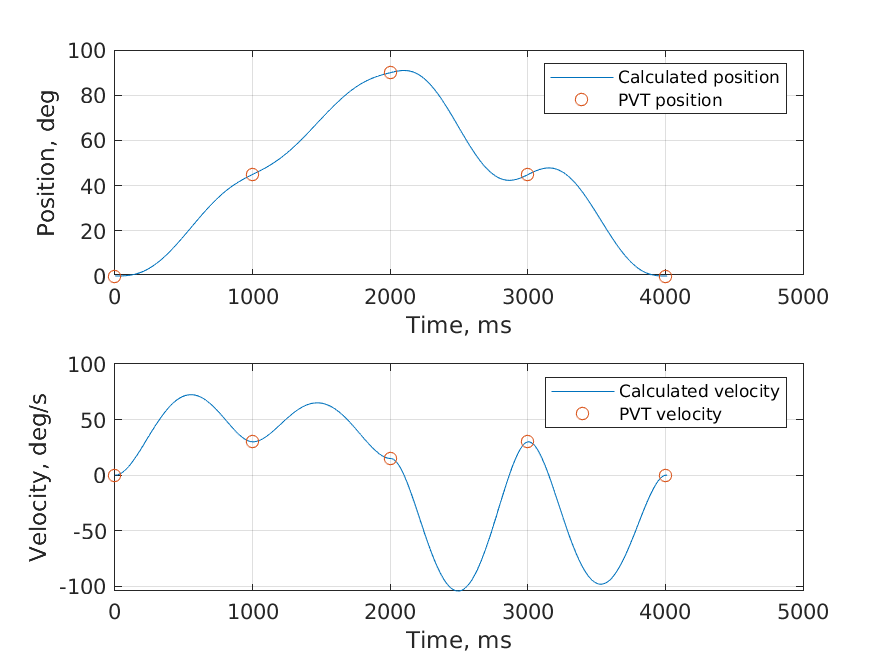
\includegraphics[width=300pt]{PVT.png}
\doxyfigcaption{Example of calculated trajectory using PVT points}
\end{DoxyImage}
 Created PVT points are arranged into a motion queue that defines the motion trajectory of the specified servo. To execute the motion queue, use the \mbox{\hyperlink{group___trajectory_ga639ef9f16dd649cbedfd65daca35ee18}{rr\+\_\+start\+\_\+motion}} function.~\newline
 When any of the parameter values (e.\+g., position, velocity) exceeds user-\/defined limits or the servo motor specifications whichever is the smallest value), the function returns an error.~\newline
~\newline


{\bfseries{Note\+:}} When you set a PVT trajectory to move more than one servo simultaneously, mind that the clock rate of the servos can differ by up to 2-\/3\%. Therefore, if the preset PVT trajectory is rather long, servos can get desynchronized. To avoid the desynchronization, we have implemented the following mechanism\+: 
\begin{DoxyItemize}
\item The device controlling the servos broadcasts a sync CAN frame to all servos on an interface. The frame should have the following format\+:~\newline
 ID = 0x27f, data = uint32 (4 bytes),~\newline
 {\bfseries{Where\+:}} ‘data’ stands for the microseconds counter value by modulus of 600,000,000, starting from any value.~\newline
 
\item Servos receive the frame and try to adjust their clock rates to that of the device using the PLL. The adjustment proper starts after the servos receive the second frame and can take up to 5 seconds, depending on the broadcasting frequency. The higher the broadcasting frequency, the less time the adjustment takes.~\newline
 
\item The broadcasting frequency is 5 Hz minimum. The recommended frequency range is from 10 to 20 Hz. When the sync frames are not broadcast or the broadcast frequency is below 5 Hz, the clock rate of servos is as usual.~\newline



\begin{DoxyParams}{Parameters}
{\em servo} & Servo descriptor returned by the \mbox{\hyperlink{group___init_ga88467da814964fd147ab9c7c7af0ed21}{rr\+\_\+init\+\_\+servo}} function \\
\hline
{\em position\+\_\+deg} & Position that the servo flange (in degrees) should reach as a result of executing the command \\
\hline
{\em velocity\+\_\+deg\+\_\+per\+\_\+sec} & Servo velocity(in degrees/sec) at the point \\
\hline
{\em time\+\_\+ms} & Time (in milliseconds) it should take the servo to move from the previous position (PVT point in a motion trajectory or an initial point) to the commanded one. The maximum admissible value is (2$^\wedge$32-\/1)/10 (roughly equivalent to 4.\+9 days). \\
\hline
\end{DoxyParams}
\begin{DoxyReturn}{Returns}
Status code (\mbox{\hyperlink{api_8h_a92d5be5038abcf89837faf85a08debdc}{rr\+\_\+ret\+\_\+status\+\_\+t}}) 
\end{DoxyReturn}

\end{DoxyItemize}\mbox{\Hypertarget{group___trajectory_ga87e6fb37af644934fad2195a7d168ca2}\label{group___trajectory_ga87e6fb37af644934fad2195a7d168ca2}} 
\index{Trajectory motion control (PVT)@{Trajectory motion control (PVT)}!rr\_add\_motion\_point\_pvat@{rr\_add\_motion\_point\_pvat}}
\index{rr\_add\_motion\_point\_pvat@{rr\_add\_motion\_point\_pvat}!Trajectory motion control (PVT)@{Trajectory motion control (PVT)}}
\doxysubsubsection{\texorpdfstring{rr\_add\_motion\_point\_pvat()}{rr\_add\_motion\_point\_pvat()}}
{\footnotesize\ttfamily \mbox{\hyperlink{api_8h_a92d5be5038abcf89837faf85a08debdc}{rr\+\_\+ret\+\_\+status\+\_\+t}} rr\+\_\+add\+\_\+motion\+\_\+point\+\_\+pvat (\begin{DoxyParamCaption}\item[{const \mbox{\hyperlink{structrr__servo__t}{rr\+\_\+servo\+\_\+t}} $\ast$}]{servo,  }\item[{const float}]{position\+\_\+deg,  }\item[{const float}]{velocity\+\_\+deg\+\_\+per\+\_\+sec,  }\item[{const float}]{accel\+\_\+deg\+\_\+per\+\_\+sec2,  }\item[{const uint32\+\_\+t}]{time\+\_\+ms }\end{DoxyParamCaption})}



The function enables creating PVAT (position-\/velocity-\/acceleration-\/time) points to set the motion trajectory of the servo specified in the \textquotesingle{}servo\textquotesingle{} parameter. PVAT points define the following\+:~\newline
 


\begin{DoxyItemize}
\item what position the servo specified in the \textquotesingle{}servo\textquotesingle{} parameter should reach~\newline
 
\item how fast the servo should move to the specified position~\newline
 
\item how long the movement to the specified position should take~\newline
 
\item with what acceleration the servo should reach the specified position
\end{DoxyItemize}For details of PVAT motion synchronization when running multiple servos, see \mbox{\hyperlink{group___trajectory_gacf26f2966a4f2035a128e1fcecd08f58}{rr\+\_\+add\+\_\+motion\+\_\+point}}. 
\begin{DoxyParams}{Parameters}
{\em servo} & Servo descriptor returned by the \mbox{\hyperlink{group___init_ga88467da814964fd147ab9c7c7af0ed21}{rr\+\_\+init\+\_\+servo}} function \\
\hline
{\em position\+\_\+deg} & Position that the servo flange (in degrees) should reach as a result of executing the command \\
\hline
{\em velocity\+\_\+deg\+\_\+per\+\_\+sec} & Servo velocity (in degrees/sec) at the point \\
\hline
{\em accel\+\_\+deg\+\_\+per\+\_\+sec2} & Servo acceleration (in degrees/sec$^\wedge$2) at the point \\
\hline
{\em time\+\_\+ms} & Time (in milliseconds) it should take the servo to move from the previous position (PVT point in a motion trajectory or an initial point) to the commanded one. The maximum admissible value is (2$^\wedge$32-\/1)/10 (roughly equivalent to 4.\+9 days). \\
\hline
\end{DoxyParams}
\begin{DoxyReturn}{Returns}
Status code (\mbox{\hyperlink{api_8h_a92d5be5038abcf89837faf85a08debdc}{rr\+\_\+ret\+\_\+status\+\_\+t}}) 
\end{DoxyReturn}
\mbox{\Hypertarget{group___trajectory_ga7a35cda046b564b51f035a81329e6906}\label{group___trajectory_ga7a35cda046b564b51f035a81329e6906}} 
\index{Trajectory motion control (PVT)@{Trajectory motion control (PVT)}!rr\_clear\_points@{rr\_clear\_points}}
\index{rr\_clear\_points@{rr\_clear\_points}!Trajectory motion control (PVT)@{Trajectory motion control (PVT)}}
\doxysubsubsection{\texorpdfstring{rr\_clear\_points()}{rr\_clear\_points()}}
{\footnotesize\ttfamily \mbox{\hyperlink{api_8h_a92d5be5038abcf89837faf85a08debdc}{rr\+\_\+ret\+\_\+status\+\_\+t}} rr\+\_\+clear\+\_\+points (\begin{DoxyParamCaption}\item[{const \mbox{\hyperlink{structrr__servo__t}{rr\+\_\+servo\+\_\+t}} $\ast$}]{servo,  }\item[{const uint32\+\_\+t}]{num\+\_\+to\+\_\+clear }\end{DoxyParamCaption})}



The function removes the number of PVT points indicated in the \textquotesingle{}num\+\_\+to\+\_\+clear\textquotesingle{} parameter from the tail of the motion queue preset for the specified servo. {\bfseries{Note\+:}} In case the indicated number of PVT points to be removed exceeds the actual remaining number of PVT points in the queue, the effect of applying the function is similar to that of applying \mbox{\hyperlink{group___trajectory_ga7b5be2d97da325eefde671c2e65e8055}{rr\+\_\+clear\+\_\+points\+\_\+all}}. 


\begin{DoxyParams}{Parameters}
{\em servo} & Servo descriptor returned by the \mbox{\hyperlink{group___init_ga88467da814964fd147ab9c7c7af0ed21}{rr\+\_\+init\+\_\+servo}} function \\
\hline
{\em num\+\_\+to\+\_\+clear} & Number of PVT points to be removed from the motion queue of the specified servo. When the parameter is set to 0, the effect of applying the function is similar to that of applying \mbox{\hyperlink{group___trajectory_ga7b5be2d97da325eefde671c2e65e8055}{rr\+\_\+clear\+\_\+points\+\_\+all}}. \\
\hline
\end{DoxyParams}
\begin{DoxyReturn}{Returns}
Status code (\mbox{\hyperlink{api_8h_a92d5be5038abcf89837faf85a08debdc}{rr\+\_\+ret\+\_\+status\+\_\+t}}) 
\end{DoxyReturn}
\mbox{\Hypertarget{group___trajectory_ga7b5be2d97da325eefde671c2e65e8055}\label{group___trajectory_ga7b5be2d97da325eefde671c2e65e8055}} 
\index{Trajectory motion control (PVT)@{Trajectory motion control (PVT)}!rr\_clear\_points\_all@{rr\_clear\_points\_all}}
\index{rr\_clear\_points\_all@{rr\_clear\_points\_all}!Trajectory motion control (PVT)@{Trajectory motion control (PVT)}}
\doxysubsubsection{\texorpdfstring{rr\_clear\_points\_all()}{rr\_clear\_points\_all()}}
{\footnotesize\ttfamily \mbox{\hyperlink{api_8h_a92d5be5038abcf89837faf85a08debdc}{rr\+\_\+ret\+\_\+status\+\_\+t}} rr\+\_\+clear\+\_\+points\+\_\+all (\begin{DoxyParamCaption}\item[{const \mbox{\hyperlink{structrr__servo__t}{rr\+\_\+servo\+\_\+t}} $\ast$}]{servo }\end{DoxyParamCaption})}



The function clears the entire motion queue of the servo specified in the \textquotesingle{}servo\textquotesingle{} parameter of the function. If you call the function while the servo is executing a motion point command, the servo stops without completing the motion. All the remaining motion points, including the one where the servo has been moving, are removed from the queue. 


\begin{DoxyParams}{Parameters}
{\em servo} & Servo descriptor returned by the \mbox{\hyperlink{group___init_ga88467da814964fd147ab9c7c7af0ed21}{rr\+\_\+init\+\_\+servo}} function \\
\hline
\end{DoxyParams}
\begin{DoxyReturn}{Returns}
Status code (\mbox{\hyperlink{api_8h_a92d5be5038abcf89837faf85a08debdc}{rr\+\_\+ret\+\_\+status\+\_\+t}}) 
\end{DoxyReturn}
\mbox{\Hypertarget{group___trajectory_ga801e9d1c29dbf5898b04cb400a8b2cad}\label{group___trajectory_ga801e9d1c29dbf5898b04cb400a8b2cad}} 
\index{Trajectory motion control (PVT)@{Trajectory motion control (PVT)}!rr\_get\_points\_free\_space@{rr\_get\_points\_free\_space}}
\index{rr\_get\_points\_free\_space@{rr\_get\_points\_free\_space}!Trajectory motion control (PVT)@{Trajectory motion control (PVT)}}
\doxysubsubsection{\texorpdfstring{rr\_get\_points\_free\_space()}{rr\_get\_points\_free\_space()}}
{\footnotesize\ttfamily \mbox{\hyperlink{api_8h_a92d5be5038abcf89837faf85a08debdc}{rr\+\_\+ret\+\_\+status\+\_\+t}} rr\+\_\+get\+\_\+points\+\_\+free\+\_\+space (\begin{DoxyParamCaption}\item[{const \mbox{\hyperlink{structrr__servo__t}{rr\+\_\+servo\+\_\+t}} $\ast$}]{servo,  }\item[{uint32\+\_\+t $\ast$}]{num }\end{DoxyParamCaption})}



The function returns how many more PVT points the user can add to the motion queue of the servo specified in the \textquotesingle{}servo\textquotesingle{} parameter. 

{\bfseries{Note\+:}} Currently, the maximum motion queue size is 100 PVT.


\begin{DoxyParams}{Parameters}
{\em servo} & Servo descriptor returned by the \mbox{\hyperlink{group___init_ga88467da814964fd147ab9c7c7af0ed21}{rr\+\_\+init\+\_\+servo}} function \\
\hline
{\em num} & Pointer to the variable where the function will save the reading \\
\hline
\end{DoxyParams}
\begin{DoxyReturn}{Returns}
Status code (\mbox{\hyperlink{api_8h_a92d5be5038abcf89837faf85a08debdc}{rr\+\_\+ret\+\_\+status\+\_\+t}}) 
\end{DoxyReturn}
\mbox{\Hypertarget{group___trajectory_ga1a62e45140604aa19ceab615536e787c}\label{group___trajectory_ga1a62e45140604aa19ceab615536e787c}} 
\index{Trajectory motion control (PVT)@{Trajectory motion control (PVT)}!rr\_get\_points\_size@{rr\_get\_points\_size}}
\index{rr\_get\_points\_size@{rr\_get\_points\_size}!Trajectory motion control (PVT)@{Trajectory motion control (PVT)}}
\doxysubsubsection{\texorpdfstring{rr\_get\_points\_size()}{rr\_get\_points\_size()}}
{\footnotesize\ttfamily \mbox{\hyperlink{api_8h_a92d5be5038abcf89837faf85a08debdc}{rr\+\_\+ret\+\_\+status\+\_\+t}} rr\+\_\+get\+\_\+points\+\_\+size (\begin{DoxyParamCaption}\item[{const \mbox{\hyperlink{structrr__servo__t}{rr\+\_\+servo\+\_\+t}} $\ast$}]{servo,  }\item[{uint32\+\_\+t $\ast$}]{num }\end{DoxyParamCaption})}



The function returns the actual motion queue size of the specified servo. The return value indicates how many PVT points have already been added to the motion queue. 


\begin{DoxyParams}{Parameters}
{\em servo} & Servo descriptor returned by the \mbox{\hyperlink{group___init_ga88467da814964fd147ab9c7c7af0ed21}{rr\+\_\+init\+\_\+servo}} function \\
\hline
{\em num} & Pointer to the parameter where the function will save the reading \\
\hline
\end{DoxyParams}
\begin{DoxyReturn}{Returns}
Status code (\mbox{\hyperlink{api_8h_a92d5be5038abcf89837faf85a08debdc}{rr\+\_\+ret\+\_\+status\+\_\+t}}) 
\end{DoxyReturn}
\mbox{\Hypertarget{group___trajectory_gaff774ce46f1685654a914b83cd04d7f1}\label{group___trajectory_gaff774ce46f1685654a914b83cd04d7f1}} 
\index{Trajectory motion control (PVT)@{Trajectory motion control (PVT)}!rr\_invoke\_time\_calculation@{rr\_invoke\_time\_calculation}}
\index{rr\_invoke\_time\_calculation@{rr\_invoke\_time\_calculation}!Trajectory motion control (PVT)@{Trajectory motion control (PVT)}}
\doxysubsubsection{\texorpdfstring{rr\_invoke\_time\_calculation()}{rr\_invoke\_time\_calculation()}}
{\footnotesize\ttfamily \mbox{\hyperlink{api_8h_a92d5be5038abcf89837faf85a08debdc}{rr\+\_\+ret\+\_\+status\+\_\+t}} rr\+\_\+invoke\+\_\+time\+\_\+calculation (\begin{DoxyParamCaption}\item[{const \mbox{\hyperlink{structrr__servo__t}{rr\+\_\+servo\+\_\+t}} $\ast$}]{servo,  }\item[{const float}]{start\+\_\+position\+\_\+deg,  }\item[{const float}]{start\+\_\+velocity\+\_\+deg\+\_\+per\+\_\+sec,  }\item[{const float}]{start\+\_\+acceleration\+\_\+deg\+\_\+per\+\_\+sec2,  }\item[{const uint32\+\_\+t}]{start\+\_\+time\+\_\+ms,  }\item[{const float}]{end\+\_\+position\+\_\+deg,  }\item[{const float}]{end\+\_\+velocity\+\_\+deg\+\_\+per\+\_\+sec,  }\item[{const float}]{end\+\_\+acceleration\+\_\+deg\+\_\+per\+\_\+sec2,  }\item[{const uint32\+\_\+t}]{end\+\_\+time\+\_\+ms,  }\item[{uint32\+\_\+t $\ast$}]{time\+\_\+ms }\end{DoxyParamCaption})}



The function enables calculating the time it will take for the specified servo to get from one position to another at the specified motion parameters (e.\+g., velocity, acceleration). {\bfseries{Note\+:}}The function is executed without the servo moving.~\newline
 

When the start time and the end time parameters are set to 0, the function returns the calculated time value. When the parameters are set to values other than 0, the function will either return OK or an error. \textquotesingle{}OK\textquotesingle{} means the motion at the specified function parameters is possible, whereas an error indicates that the motion cannot be executed.


\begin{DoxyParams}{Parameters}
{\em servo} & Servo descriptor returned by the \mbox{\hyperlink{group___init_ga88467da814964fd147ab9c7c7af0ed21}{rr\+\_\+init\+\_\+servo}} function \\
\hline
{\em start\+\_\+position\+\_\+deg} & Position (in degrees) from where the specified servo should start moving \\
\hline
{\em start\+\_\+velocity\+\_\+deg\+\_\+per\+\_\+sec} & Servo velocity (in degrees/sec) at the start of motion \\
\hline
{\em start\+\_\+acceleration\+\_\+deg\+\_\+per\+\_\+sec2} & Servo acceleration (in degrees/sec$^\wedge$2) at the start of motion \\
\hline
{\em start\+\_\+time\+\_\+ms} & Initial time setting (in milliseconds) \\
\hline
{\em end\+\_\+position\+\_\+deg} & Position (in degrees) where the servo should arrive \\
\hline
{\em end\+\_\+velocity\+\_\+deg\+\_\+per\+\_\+sec} & Servo velocity (in degrees/sec) in the end of motion \\
\hline
{\em end\+\_\+acceleration\+\_\+deg\+\_\+per\+\_\+sec2} & Servo acceleration (in degrees/sec$^\wedge$2) in the end of motion \\
\hline
{\em end\+\_\+time\+\_\+ms} & Final time setting (in milliseconds) \\
\hline
{\em time\+\_\+ms} & Pointer to the variable where the function will save the calculated time \\
\hline
\end{DoxyParams}
\begin{DoxyReturn}{Returns}
Status code (\mbox{\hyperlink{api_8h_a92d5be5038abcf89837faf85a08debdc}{rr\+\_\+ret\+\_\+status\+\_\+t}}) 
\end{DoxyReturn}
\mbox{\Hypertarget{group___trajectory_ga639ef9f16dd649cbedfd65daca35ee18}\label{group___trajectory_ga639ef9f16dd649cbedfd65daca35ee18}} 
\index{Trajectory motion control (PVT)@{Trajectory motion control (PVT)}!rr\_start\_motion@{rr\_start\_motion}}
\index{rr\_start\_motion@{rr\_start\_motion}!Trajectory motion control (PVT)@{Trajectory motion control (PVT)}}
\doxysubsubsection{\texorpdfstring{rr\_start\_motion()}{rr\_start\_motion()}}
{\footnotesize\ttfamily \mbox{\hyperlink{api_8h_a92d5be5038abcf89837faf85a08debdc}{rr\+\_\+ret\+\_\+status\+\_\+t}} rr\+\_\+start\+\_\+motion (\begin{DoxyParamCaption}\item[{\mbox{\hyperlink{structrr__can__interface__t}{rr\+\_\+can\+\_\+interface\+\_\+t}} $\ast$}]{iface,  }\item[{uint32\+\_\+t}]{timestamp\+\_\+ms }\end{DoxyParamCaption})}



The function commands all servos connected to the specified interface (CAN bus) to move simultaneously through a number of preset PVT points (see \mbox{\hyperlink{group___trajectory_gacf26f2966a4f2035a128e1fcecd08f58}{rr\+\_\+add\+\_\+motion\+\_\+point}}).~\newline
 

{\bfseries{Note\+:}} When any of the servos fails to reach any of the PVT points due to an error, it will broadcast a \char`\"{}\+Go to Stopped State\char`\"{} command to all the other servos on the same bus. The servos will stop executing the preset PVT points and go to the stopped state. In the state, only Heartbeats are available. You can neither communicate with servos nor command them to execute any operations.

{\bfseries{Note\+:}} Once servos execute the last PVT in their preset motion queue, the queue is cleared automatically.


\begin{DoxyParams}{Parameters}
{\em iface} & Interface descriptor returned by the \mbox{\hyperlink{group___init_ga472a4890dcc7d7a13123c56a06946d91}{rr\+\_\+init\+\_\+interface}} function \\
\hline
{\em timestamp\+\_\+ms} & Delay (in milliseconds) before the servos associated with the interface start to move. When the value is set to 0, the servos will start moving immediately. The available value range is from 0 to 2$^\wedge$24-\/1. \\
\hline
\end{DoxyParams}
\begin{DoxyReturn}{Returns}
Status code (\mbox{\hyperlink{api_8h_a92d5be5038abcf89837faf85a08debdc}{rr\+\_\+ret\+\_\+status\+\_\+t}}) 
\end{DoxyReturn}

\hypertarget{group___config}{}\doxysection{Reading and writing servo configuration}
\label{group___config}\index{Reading and writing servo configuration@{Reading and writing servo configuration}}
\doxysubsection*{Functions}
\begin{DoxyCompactItemize}
\item 
\mbox{\hyperlink{api_8h_a92d5be5038abcf89837faf85a08debdc}{rr\+\_\+ret\+\_\+status\+\_\+t}} \mbox{\hyperlink{group___config_gad266a0b3e3e349bbb40e5791d35093be}{rr\+\_\+set\+\_\+zero\+\_\+position}} (const \mbox{\hyperlink{structrr__servo__t}{rr\+\_\+servo\+\_\+t}} $\ast$servo, const float position\+\_\+deg)
\begin{DoxyCompactList}\small\item\em The function enables setting the current position (in degrees) of the servo with the specified descriptor to any value defined by the user. For instance, when the current servo position is 101 degrees and the \textquotesingle{}position\+\_\+deg\textquotesingle{} parameter is set to 25 degrees, the servo is assumed to be positioned at 25 degrees. \end{DoxyCompactList}\item 
\mbox{\hyperlink{api_8h_a92d5be5038abcf89837faf85a08debdc}{rr\+\_\+ret\+\_\+status\+\_\+t}} \mbox{\hyperlink{group___config_ga16d3d1e2d5e973706f1735b4b55d6b9c}{rr\+\_\+set\+\_\+zero\+\_\+position\+\_\+and\+\_\+save}} (const \mbox{\hyperlink{structrr__servo__t}{rr\+\_\+servo\+\_\+t}} $\ast$servo, const float position\+\_\+deg)
\begin{DoxyCompactList}\small\item\em The function enables setting the current position (in degrees) of the servo with the specified descriptor to any value defined by the user and saving it to the FLASH memory. If you don\textquotesingle{}t want to save the newly set position, use the \mbox{\hyperlink{group___config_gad266a0b3e3e349bbb40e5791d35093be}{rr\+\_\+set\+\_\+zero\+\_\+position}} function.~\newline
 \end{DoxyCompactList}\item 
\mbox{\hyperlink{api_8h_a92d5be5038abcf89837faf85a08debdc}{rr\+\_\+ret\+\_\+status\+\_\+t}} \mbox{\hyperlink{group___config_ga3fbab9a19159bdcd53d7a4b061848c2b}{rr\+\_\+get\+\_\+max\+\_\+velocity}} (const \mbox{\hyperlink{structrr__servo__t}{rr\+\_\+servo\+\_\+t}} $\ast$servo, float $\ast$velocity\+\_\+deg\+\_\+per\+\_\+sec)
\begin{DoxyCompactList}\small\item\em The function reads the maximum velocity of the servo at the current moment. It returns the smallest of the three values—the user-\/defined maximum velocity limit (\mbox{\hyperlink{group___config_ga52736c105da7440077f2dcb67388dc47}{rr\+\_\+set\+\_\+max\+\_\+velocity}}), the maximum velocity value based on the servo specifications, or the calculated maximum velocity based on the supply voltage. \end{DoxyCompactList}\item 
\mbox{\hyperlink{api_8h_a92d5be5038abcf89837faf85a08debdc}{rr\+\_\+ret\+\_\+status\+\_\+t}} \mbox{\hyperlink{group___config_ga52736c105da7440077f2dcb67388dc47}{rr\+\_\+set\+\_\+max\+\_\+velocity}} (const \mbox{\hyperlink{structrr__servo__t}{rr\+\_\+servo\+\_\+t}} $\ast$servo, const float max\+\_\+velocity\+\_\+deg\+\_\+per\+\_\+sec)
\begin{DoxyCompactList}\small\item\em The function sets the maximum velocity limit for the servo specified in the \textquotesingle{}servo\textquotesingle{} parameter. The setting is volatile\+: after a reset or a power outage, it is no longer valid. \end{DoxyCompactList}\end{DoxyCompactItemize}


\doxysubsection{Detailed Description}


\doxysubsection{Function Documentation}
\mbox{\Hypertarget{group___config_ga3fbab9a19159bdcd53d7a4b061848c2b}\label{group___config_ga3fbab9a19159bdcd53d7a4b061848c2b}} 
\index{Reading and writing servo configuration@{Reading and writing servo configuration}!rr\_get\_max\_velocity@{rr\_get\_max\_velocity}}
\index{rr\_get\_max\_velocity@{rr\_get\_max\_velocity}!Reading and writing servo configuration@{Reading and writing servo configuration}}
\doxysubsubsection{\texorpdfstring{rr\_get\_max\_velocity()}{rr\_get\_max\_velocity()}}
{\footnotesize\ttfamily \mbox{\hyperlink{api_8h_a92d5be5038abcf89837faf85a08debdc}{rr\+\_\+ret\+\_\+status\+\_\+t}} rr\+\_\+get\+\_\+max\+\_\+velocity (\begin{DoxyParamCaption}\item[{const \mbox{\hyperlink{structrr__servo__t}{rr\+\_\+servo\+\_\+t}} $\ast$}]{servo,  }\item[{float $\ast$}]{velocity\+\_\+deg\+\_\+per\+\_\+sec }\end{DoxyParamCaption})}



The function reads the maximum velocity of the servo at the current moment. It returns the smallest of the three values—the user-\/defined maximum velocity limit (\mbox{\hyperlink{group___config_ga52736c105da7440077f2dcb67388dc47}{rr\+\_\+set\+\_\+max\+\_\+velocity}}), the maximum velocity value based on the servo specifications, or the calculated maximum velocity based on the supply voltage. 


\begin{DoxyParams}{Parameters}
{\em servo} & Servo descriptor returned by the \mbox{\hyperlink{group___init_ga88467da814964fd147ab9c7c7af0ed21}{rr\+\_\+init\+\_\+servo}} function \\
\hline
{\em velocity\+\_\+deg\+\_\+per\+\_\+sec} & Maximum servo velocity (in degrees/sec) \\
\hline
\end{DoxyParams}
\begin{DoxyReturn}{Returns}
Status code (\mbox{\hyperlink{api_8h_a92d5be5038abcf89837faf85a08debdc}{rr\+\_\+ret\+\_\+status\+\_\+t}}) 
\end{DoxyReturn}
\mbox{\Hypertarget{group___config_ga52736c105da7440077f2dcb67388dc47}\label{group___config_ga52736c105da7440077f2dcb67388dc47}} 
\index{Reading and writing servo configuration@{Reading and writing servo configuration}!rr\_set\_max\_velocity@{rr\_set\_max\_velocity}}
\index{rr\_set\_max\_velocity@{rr\_set\_max\_velocity}!Reading and writing servo configuration@{Reading and writing servo configuration}}
\doxysubsubsection{\texorpdfstring{rr\_set\_max\_velocity()}{rr\_set\_max\_velocity()}}
{\footnotesize\ttfamily \mbox{\hyperlink{api_8h_a92d5be5038abcf89837faf85a08debdc}{rr\+\_\+ret\+\_\+status\+\_\+t}} rr\+\_\+set\+\_\+max\+\_\+velocity (\begin{DoxyParamCaption}\item[{const \mbox{\hyperlink{structrr__servo__t}{rr\+\_\+servo\+\_\+t}} $\ast$}]{servo,  }\item[{const float}]{max\+\_\+velocity\+\_\+deg\+\_\+per\+\_\+sec }\end{DoxyParamCaption})}



The function sets the maximum velocity limit for the servo specified in the \textquotesingle{}servo\textquotesingle{} parameter. The setting is volatile\+: after a reset or a power outage, it is no longer valid. 


\begin{DoxyParams}{Parameters}
{\em servo} & Servo descriptor returned by the \mbox{\hyperlink{group___init_ga88467da814964fd147ab9c7c7af0ed21}{rr\+\_\+init\+\_\+servo}} function \\
\hline
{\em max\+\_\+velocity\+\_\+deg\+\_\+per\+\_\+sec} & Velocity at the servo flange (in degrees/sec) \\
\hline
\end{DoxyParams}
\begin{DoxyReturn}{Returns}
Status code (\mbox{\hyperlink{api_8h_a92d5be5038abcf89837faf85a08debdc}{rr\+\_\+ret\+\_\+status\+\_\+t}}) 
\end{DoxyReturn}
\mbox{\Hypertarget{group___config_gad266a0b3e3e349bbb40e5791d35093be}\label{group___config_gad266a0b3e3e349bbb40e5791d35093be}} 
\index{Reading and writing servo configuration@{Reading and writing servo configuration}!rr\_set\_zero\_position@{rr\_set\_zero\_position}}
\index{rr\_set\_zero\_position@{rr\_set\_zero\_position}!Reading and writing servo configuration@{Reading and writing servo configuration}}
\doxysubsubsection{\texorpdfstring{rr\_set\_zero\_position()}{rr\_set\_zero\_position()}}
{\footnotesize\ttfamily \mbox{\hyperlink{api_8h_a92d5be5038abcf89837faf85a08debdc}{rr\+\_\+ret\+\_\+status\+\_\+t}} rr\+\_\+set\+\_\+zero\+\_\+position (\begin{DoxyParamCaption}\item[{const \mbox{\hyperlink{structrr__servo__t}{rr\+\_\+servo\+\_\+t}} $\ast$}]{servo,  }\item[{const float}]{position\+\_\+deg }\end{DoxyParamCaption})}



The function enables setting the current position (in degrees) of the servo with the specified descriptor to any value defined by the user. For instance, when the current servo position is 101 degrees and the \textquotesingle{}position\+\_\+deg\textquotesingle{} parameter is set to 25 degrees, the servo is assumed to be positioned at 25 degrees. 

The setting is volatile\+: after a reset or a power outage, it is no longer valid.


\begin{DoxyParams}{Parameters}
{\em servo} & Servo descriptor returned by the \mbox{\hyperlink{group___init_ga88467da814964fd147ab9c7c7af0ed21}{rr\+\_\+init\+\_\+servo}} function \\
\hline
{\em position\+\_\+deg} & User-\/defined position (in degrees) to replace the current position value \\
\hline
\end{DoxyParams}
\begin{DoxyReturn}{Returns}
Status code (\mbox{\hyperlink{api_8h_a92d5be5038abcf89837faf85a08debdc}{rr\+\_\+ret\+\_\+status\+\_\+t}}) 
\end{DoxyReturn}
\mbox{\Hypertarget{group___config_ga16d3d1e2d5e973706f1735b4b55d6b9c}\label{group___config_ga16d3d1e2d5e973706f1735b4b55d6b9c}} 
\index{Reading and writing servo configuration@{Reading and writing servo configuration}!rr\_set\_zero\_position\_and\_save@{rr\_set\_zero\_position\_and\_save}}
\index{rr\_set\_zero\_position\_and\_save@{rr\_set\_zero\_position\_and\_save}!Reading and writing servo configuration@{Reading and writing servo configuration}}
\doxysubsubsection{\texorpdfstring{rr\_set\_zero\_position\_and\_save()}{rr\_set\_zero\_position\_and\_save()}}
{\footnotesize\ttfamily \mbox{\hyperlink{api_8h_a92d5be5038abcf89837faf85a08debdc}{rr\+\_\+ret\+\_\+status\+\_\+t}} rr\+\_\+set\+\_\+zero\+\_\+position\+\_\+and\+\_\+save (\begin{DoxyParamCaption}\item[{const \mbox{\hyperlink{structrr__servo__t}{rr\+\_\+servo\+\_\+t}} $\ast$}]{servo,  }\item[{const float}]{position\+\_\+deg }\end{DoxyParamCaption})}



The function enables setting the current position (in degrees) of the servo with the specified descriptor to any value defined by the user and saving it to the FLASH memory. If you don\textquotesingle{}t want to save the newly set position, use the \mbox{\hyperlink{group___config_gad266a0b3e3e349bbb40e5791d35093be}{rr\+\_\+set\+\_\+zero\+\_\+position}} function.~\newline
 

{\bfseries{Note\+:}}The FLASH memory limit is 1,000 write cycles. Therefore, it is not advisable to use the function on a regular basis.


\begin{DoxyParams}{Parameters}
{\em servo} & Servo descriptor returned by the \mbox{\hyperlink{group___init_ga88467da814964fd147ab9c7c7af0ed21}{rr\+\_\+init\+\_\+servo}} function \\
\hline
{\em position\+\_\+deg} & User-\/defined position (in degrees) to replace the current position value \\
\hline
\end{DoxyParams}
\begin{DoxyReturn}{Returns}
Status code (\mbox{\hyperlink{api_8h_a92d5be5038abcf89837faf85a08debdc}{rr\+\_\+ret\+\_\+status\+\_\+t}}) 
\end{DoxyReturn}

\hypertarget{group___realtime}{}\doxysection{Reading realtime parameters}
\label{group___realtime}\index{Reading realtime parameters@{Reading realtime parameters}}
\doxysubsection*{Functions}
\begin{DoxyCompactItemize}
\item 
\mbox{\hyperlink{api_8h_a92d5be5038abcf89837faf85a08debdc}{rr\+\_\+ret\+\_\+status\+\_\+t}} \mbox{\hyperlink{group___realtime_ga95a1707406a0cb3f665a4ee529d066f5}{rr\+\_\+param\+\_\+cache\+\_\+update}} (\mbox{\hyperlink{structrr__servo__t}{rr\+\_\+servo\+\_\+t}} $\ast$servo)
\begin{DoxyCompactList}\small\item\em The function is always used in combination with the \mbox{\hyperlink{group___realtime_ga49c6107db464d0ece3dbc9d590942f54}{rr\+\_\+param\+\_\+cache\+\_\+setup\+\_\+entry}} function. It retreives from the servo the array of parameters that was set up using \mbox{\hyperlink{group___realtime_ga49c6107db464d0ece3dbc9d590942f54}{rr\+\_\+param\+\_\+cache\+\_\+setup\+\_\+entry}} function and saves the array to the program cache. You can subsequently read the parameters from the program cache with the \mbox{\hyperlink{group___realtime_ga4e21be75a34c6d2862e6d78e6add4c2a}{rr\+\_\+read\+\_\+cached\+\_\+parameter}} function. For more information, see \mbox{\hyperlink{group___realtime_ga49c6107db464d0ece3dbc9d590942f54}{rr\+\_\+param\+\_\+cache\+\_\+setup\+\_\+entry}}. \end{DoxyCompactList}\item 
\mbox{\hyperlink{api_8h_a92d5be5038abcf89837faf85a08debdc}{rr\+\_\+ret\+\_\+status\+\_\+t}} \mbox{\hyperlink{group___realtime_gaf070f53f5fb1597821794840746cd897}{rr\+\_\+param\+\_\+cache\+\_\+update\+\_\+with\+\_\+timestamp}} (\mbox{\hyperlink{structrr__servo__t}{rr\+\_\+servo\+\_\+t}} $\ast$servo)
\begin{DoxyCompactList}\small\item\em Same as \mbox{\hyperlink{group___realtime_ga95a1707406a0cb3f665a4ee529d066f5}{rr\+\_\+param\+\_\+cache\+\_\+update}} but with timestamp functionality. \end{DoxyCompactList}\item 
\mbox{\hyperlink{api_8h_a92d5be5038abcf89837faf85a08debdc}{rr\+\_\+ret\+\_\+status\+\_\+t}} \mbox{\hyperlink{group___realtime_ga49c6107db464d0ece3dbc9d590942f54}{rr\+\_\+param\+\_\+cache\+\_\+setup\+\_\+entry}} (\mbox{\hyperlink{structrr__servo__t}{rr\+\_\+servo\+\_\+t}} $\ast$servo, const \mbox{\hyperlink{api_8h_aa1f58887fab4642cf49f6f453c1d276d}{rr\+\_\+servo\+\_\+param\+\_\+t}} param, bool enabled)
\begin{DoxyCompactList}\small\item\em The function is the fist one in the API call sequence that enables reading multiple servo paramaters (e.\+g., velocity, voltage, and position) as a data array. Using the sequence is advisable when you need to read {\bfseries{more than one parameter at a time}}. The user can set up the array to include up to 50 parameters. In all, the sequence comprises the following functions\+: \end{DoxyCompactList}\item 
\mbox{\hyperlink{api_8h_a92d5be5038abcf89837faf85a08debdc}{rr\+\_\+ret\+\_\+status\+\_\+t}} \mbox{\hyperlink{group___realtime_ga4e21e268034d9564da77bc23004fc56c}{rr\+\_\+read\+\_\+parameter}} (\mbox{\hyperlink{structrr__servo__t}{rr\+\_\+servo\+\_\+t}} $\ast$servo, const \mbox{\hyperlink{api_8h_aa1f58887fab4642cf49f6f453c1d276d}{rr\+\_\+servo\+\_\+param\+\_\+t}} param, float $\ast$value)
\begin{DoxyCompactList}\small\item\em The function enables reading a single parameter directly from the servo specified in the \textquotesingle{}servo\textquotesingle{} parameter of the function. The function returns the current value of the parameter. Additionally, the parameter is saved to the program cache, irrespective of whether it was enabled/ disabled with the \mbox{\hyperlink{group___realtime_ga49c6107db464d0ece3dbc9d590942f54}{rr\+\_\+param\+\_\+cache\+\_\+setup\+\_\+entry}} function. \end{DoxyCompactList}\item 
\mbox{\hyperlink{api_8h_a92d5be5038abcf89837faf85a08debdc}{rr\+\_\+ret\+\_\+status\+\_\+t}} \mbox{\hyperlink{group___realtime_ga582ec862f311c55bab380830eae5d3bc}{rr\+\_\+read\+\_\+parameter\+\_\+with\+\_\+timestamp}} (\mbox{\hyperlink{structrr__servo__t}{rr\+\_\+servo\+\_\+t}} $\ast$servo, const \mbox{\hyperlink{api_8h_aa1f58887fab4642cf49f6f453c1d276d}{rr\+\_\+servo\+\_\+param\+\_\+t}} param, float $\ast$value, uint32\+\_\+t $\ast$timestamp)
\begin{DoxyCompactList}\small\item\em Same \mbox{\hyperlink{group___realtime_ga4e21e268034d9564da77bc23004fc56c}{rr\+\_\+read\+\_\+parameter}} but with timestamp functionality. \end{DoxyCompactList}\item 
\mbox{\hyperlink{api_8h_a92d5be5038abcf89837faf85a08debdc}{rr\+\_\+ret\+\_\+status\+\_\+t}} \mbox{\hyperlink{group___realtime_ga4e21be75a34c6d2862e6d78e6add4c2a}{rr\+\_\+read\+\_\+cached\+\_\+parameter}} (\mbox{\hyperlink{structrr__servo__t}{rr\+\_\+servo\+\_\+t}} $\ast$servo, const \mbox{\hyperlink{api_8h_aa1f58887fab4642cf49f6f453c1d276d}{rr\+\_\+servo\+\_\+param\+\_\+t}} param, float $\ast$value)
\begin{DoxyCompactList}\small\item\em The function is always used in combination with the \mbox{\hyperlink{group___realtime_ga49c6107db464d0ece3dbc9d590942f54}{rr\+\_\+param\+\_\+cache\+\_\+setup\+\_\+entry}} and the \mbox{\hyperlink{group___realtime_ga95a1707406a0cb3f665a4ee529d066f5}{rr\+\_\+param\+\_\+cache\+\_\+update}} functions. For more information, see \mbox{\hyperlink{group___realtime_ga49c6107db464d0ece3dbc9d590942f54}{rr\+\_\+param\+\_\+cache\+\_\+setup\+\_\+entry}}. \end{DoxyCompactList}\item 
\mbox{\hyperlink{api_8h_a92d5be5038abcf89837faf85a08debdc}{rr\+\_\+ret\+\_\+status\+\_\+t}} \mbox{\hyperlink{group___realtime_gaca9055c4e8d07427a28d45e8fc870d5a}{rr\+\_\+read\+\_\+cached\+\_\+parameter\+\_\+with\+\_\+timestamp}} (\mbox{\hyperlink{structrr__servo__t}{rr\+\_\+servo\+\_\+t}} $\ast$servo, const \mbox{\hyperlink{api_8h_aa1f58887fab4642cf49f6f453c1d276d}{rr\+\_\+servo\+\_\+param\+\_\+t}} param, float $\ast$value, uint32\+\_\+t $\ast$timestamp)
\begin{DoxyCompactList}\small\item\em Same as \mbox{\hyperlink{group___realtime_ga4e21be75a34c6d2862e6d78e6add4c2a}{rr\+\_\+read\+\_\+cached\+\_\+parameter}} but with timestamp functionality. \end{DoxyCompactList}\end{DoxyCompactItemize}


\doxysubsection{Detailed Description}


\doxysubsection{Function Documentation}
\mbox{\Hypertarget{group___realtime_ga49c6107db464d0ece3dbc9d590942f54}\label{group___realtime_ga49c6107db464d0ece3dbc9d590942f54}} 
\index{Reading realtime parameters@{Reading realtime parameters}!rr\_param\_cache\_setup\_entry@{rr\_param\_cache\_setup\_entry}}
\index{rr\_param\_cache\_setup\_entry@{rr\_param\_cache\_setup\_entry}!Reading realtime parameters@{Reading realtime parameters}}
\doxysubsubsection{\texorpdfstring{rr\_param\_cache\_setup\_entry()}{rr\_param\_cache\_setup\_entry()}}
{\footnotesize\ttfamily \mbox{\hyperlink{api_8h_a92d5be5038abcf89837faf85a08debdc}{rr\+\_\+ret\+\_\+status\+\_\+t}} rr\+\_\+param\+\_\+cache\+\_\+setup\+\_\+entry (\begin{DoxyParamCaption}\item[{\mbox{\hyperlink{structrr__servo__t}{rr\+\_\+servo\+\_\+t}} $\ast$}]{servo,  }\item[{const \mbox{\hyperlink{api_8h_aa1f58887fab4642cf49f6f453c1d276d}{rr\+\_\+servo\+\_\+param\+\_\+t}}}]{param,  }\item[{bool}]{enabled }\end{DoxyParamCaption})}



The function is the fist one in the API call sequence that enables reading multiple servo paramaters (e.\+g., velocity, voltage, and position) as a data array. Using the sequence is advisable when you need to read {\bfseries{more than one parameter at a time}}. The user can set up the array to include up to 50 parameters. In all, the sequence comprises the following functions\+: 


\begin{DoxyItemize}
\item \mbox{\hyperlink{group___realtime_ga49c6107db464d0ece3dbc9d590942f54}{rr\+\_\+param\+\_\+cache\+\_\+setup\+\_\+entry}} for setting up an array of servo parameters to read 
\item \mbox{\hyperlink{group___realtime_ga95a1707406a0cb3f665a4ee529d066f5}{rr\+\_\+param\+\_\+cache\+\_\+update}} for retreiving the parameters from the servo and saving them to the program cache 
\item \mbox{\hyperlink{group___realtime_ga4e21be75a34c6d2862e6d78e6add4c2a}{rr\+\_\+read\+\_\+cached\+\_\+parameter}} for reading parameters from the program cache
\end{DoxyItemize}Using the sequence of API calls allows for speeding up data acquisition by nearly two times. Let\textquotesingle{}s assume you need to read 49 parameters. At a bit rate of 1 MBit/s, reading them one by one will take about 35 ms, whereas reading them as an array will only take 10 ms. 

{\bfseries{Note\+:}} When you need to read a single parameter, it is better to use the \mbox{\hyperlink{group___realtime_ga4e21e268034d9564da77bc23004fc56c}{rr\+\_\+read\+\_\+parameter}} function.


\begin{DoxyParams}{Parameters}
{\em servo} & Servo descriptor returned by the \mbox{\hyperlink{group___init_ga88467da814964fd147ab9c7c7af0ed21}{rr\+\_\+init\+\_\+servo}} function \\
\hline
{\em param} & Index of the parameter to read as indicated in the \mbox{\hyperlink{api_8h_aa1f58887fab4642cf49f6f453c1d276d}{rr\+\_\+servo\+\_\+param\+\_\+t}} list (e.\+g., APP\+\_\+\+PARAM\+\_\+\+POSITION\+\_\+\+ROTOR) \\
\hline
{\em enabled} & Set True/\+False to enable/ disable the specified parameter for reading \\
\hline
\end{DoxyParams}
\begin{DoxyReturn}{Returns}
Status code (\mbox{\hyperlink{api_8h_a92d5be5038abcf89837faf85a08debdc}{rr\+\_\+ret\+\_\+status\+\_\+t}}) 
\end{DoxyReturn}
\mbox{\Hypertarget{group___realtime_ga95a1707406a0cb3f665a4ee529d066f5}\label{group___realtime_ga95a1707406a0cb3f665a4ee529d066f5}} 
\index{Reading realtime parameters@{Reading realtime parameters}!rr\_param\_cache\_update@{rr\_param\_cache\_update}}
\index{rr\_param\_cache\_update@{rr\_param\_cache\_update}!Reading realtime parameters@{Reading realtime parameters}}
\doxysubsubsection{\texorpdfstring{rr\_param\_cache\_update()}{rr\_param\_cache\_update()}}
{\footnotesize\ttfamily \mbox{\hyperlink{api_8h_a92d5be5038abcf89837faf85a08debdc}{rr\+\_\+ret\+\_\+status\+\_\+t}} rr\+\_\+param\+\_\+cache\+\_\+update (\begin{DoxyParamCaption}\item[{\mbox{\hyperlink{structrr__servo__t}{rr\+\_\+servo\+\_\+t}} $\ast$}]{servo }\end{DoxyParamCaption})}



The function is always used in combination with the \mbox{\hyperlink{group___realtime_ga49c6107db464d0ece3dbc9d590942f54}{rr\+\_\+param\+\_\+cache\+\_\+setup\+\_\+entry}} function. It retreives from the servo the array of parameters that was set up using \mbox{\hyperlink{group___realtime_ga49c6107db464d0ece3dbc9d590942f54}{rr\+\_\+param\+\_\+cache\+\_\+setup\+\_\+entry}} function and saves the array to the program cache. You can subsequently read the parameters from the program cache with the \mbox{\hyperlink{group___realtime_ga4e21be75a34c6d2862e6d78e6add4c2a}{rr\+\_\+read\+\_\+cached\+\_\+parameter}} function. For more information, see \mbox{\hyperlink{group___realtime_ga49c6107db464d0ece3dbc9d590942f54}{rr\+\_\+param\+\_\+cache\+\_\+setup\+\_\+entry}}. 

{\bfseries{Note}}\+: After you exit the program, the cache will be cleared.


\begin{DoxyParams}{Parameters}
{\em servo} & Servo descriptor returned by the \mbox{\hyperlink{group___init_ga88467da814964fd147ab9c7c7af0ed21}{rr\+\_\+init\+\_\+servo}} function \\
\hline
\end{DoxyParams}
\begin{DoxyReturn}{Returns}
Status code (\mbox{\hyperlink{api_8h_a92d5be5038abcf89837faf85a08debdc}{rr\+\_\+ret\+\_\+status\+\_\+t}}) 
\end{DoxyReturn}
\mbox{\Hypertarget{group___realtime_gaf070f53f5fb1597821794840746cd897}\label{group___realtime_gaf070f53f5fb1597821794840746cd897}} 
\index{Reading realtime parameters@{Reading realtime parameters}!rr\_param\_cache\_update\_with\_timestamp@{rr\_param\_cache\_update\_with\_timestamp}}
\index{rr\_param\_cache\_update\_with\_timestamp@{rr\_param\_cache\_update\_with\_timestamp}!Reading realtime parameters@{Reading realtime parameters}}
\doxysubsubsection{\texorpdfstring{rr\_param\_cache\_update\_with\_timestamp()}{rr\_param\_cache\_update\_with\_timestamp()}}
{\footnotesize\ttfamily \mbox{\hyperlink{api_8h_a92d5be5038abcf89837faf85a08debdc}{rr\+\_\+ret\+\_\+status\+\_\+t}} rr\+\_\+param\+\_\+cache\+\_\+update\+\_\+with\+\_\+timestamp (\begin{DoxyParamCaption}\item[{\mbox{\hyperlink{structrr__servo__t}{rr\+\_\+servo\+\_\+t}} $\ast$}]{servo }\end{DoxyParamCaption})}



Same as \mbox{\hyperlink{group___realtime_ga95a1707406a0cb3f665a4ee529d066f5}{rr\+\_\+param\+\_\+cache\+\_\+update}} but with timestamp functionality. 


\begin{DoxyParams}{Parameters}
{\em servo} & Servo descriptor returned by the \mbox{\hyperlink{group___init_ga88467da814964fd147ab9c7c7af0ed21}{rr\+\_\+init\+\_\+servo}} function \\
\hline
\end{DoxyParams}
\begin{DoxyReturn}{Returns}
Status code (\mbox{\hyperlink{api_8h_a92d5be5038abcf89837faf85a08debdc}{rr\+\_\+ret\+\_\+status\+\_\+t}}) 
\end{DoxyReturn}
\mbox{\Hypertarget{group___realtime_ga4e21be75a34c6d2862e6d78e6add4c2a}\label{group___realtime_ga4e21be75a34c6d2862e6d78e6add4c2a}} 
\index{Reading realtime parameters@{Reading realtime parameters}!rr\_read\_cached\_parameter@{rr\_read\_cached\_parameter}}
\index{rr\_read\_cached\_parameter@{rr\_read\_cached\_parameter}!Reading realtime parameters@{Reading realtime parameters}}
\doxysubsubsection{\texorpdfstring{rr\_read\_cached\_parameter()}{rr\_read\_cached\_parameter()}}
{\footnotesize\ttfamily \mbox{\hyperlink{api_8h_a92d5be5038abcf89837faf85a08debdc}{rr\+\_\+ret\+\_\+status\+\_\+t}} rr\+\_\+read\+\_\+cached\+\_\+parameter (\begin{DoxyParamCaption}\item[{\mbox{\hyperlink{structrr__servo__t}{rr\+\_\+servo\+\_\+t}} $\ast$}]{servo,  }\item[{const \mbox{\hyperlink{api_8h_aa1f58887fab4642cf49f6f453c1d276d}{rr\+\_\+servo\+\_\+param\+\_\+t}}}]{param,  }\item[{float $\ast$}]{value }\end{DoxyParamCaption})}



The function is always used in combination with the \mbox{\hyperlink{group___realtime_ga49c6107db464d0ece3dbc9d590942f54}{rr\+\_\+param\+\_\+cache\+\_\+setup\+\_\+entry}} and the \mbox{\hyperlink{group___realtime_ga95a1707406a0cb3f665a4ee529d066f5}{rr\+\_\+param\+\_\+cache\+\_\+update}} functions. For more information, see \mbox{\hyperlink{group___realtime_ga49c6107db464d0ece3dbc9d590942f54}{rr\+\_\+param\+\_\+cache\+\_\+setup\+\_\+entry}}. 

The function enables reading parameters from the program cache. If you want to read more than one parameter, you will need to make a separate API call for each of them.

{\bfseries{Note}}\+: Prior to reading a parameter, make sure to update the program cache using the \mbox{\hyperlink{group___realtime_ga95a1707406a0cb3f665a4ee529d066f5}{rr\+\_\+param\+\_\+cache\+\_\+update}} function. 
\begin{DoxyParams}{Parameters}
{\em servo} & Servo descriptor returned by the \mbox{\hyperlink{group___init_ga88467da814964fd147ab9c7c7af0ed21}{rr\+\_\+init\+\_\+servo}} function \\
\hline
{\em param} & Index of the parameter to read; you can find these indices in the \mbox{\hyperlink{api_8h_aa1f58887fab4642cf49f6f453c1d276d}{rr\+\_\+servo\+\_\+param\+\_\+t}} list (e.\+g., APP\+\_\+\+PARAM\+\_\+\+POSITION\+\_\+\+ROTOR) \\
\hline
{\em value} & Pointer to the variable where the function will save the reading \\
\hline
\end{DoxyParams}
\begin{DoxyReturn}{Returns}
Status code (\mbox{\hyperlink{api_8h_a92d5be5038abcf89837faf85a08debdc}{rr\+\_\+ret\+\_\+status\+\_\+t}}) 
\end{DoxyReturn}
\mbox{\Hypertarget{group___realtime_gaca9055c4e8d07427a28d45e8fc870d5a}\label{group___realtime_gaca9055c4e8d07427a28d45e8fc870d5a}} 
\index{Reading realtime parameters@{Reading realtime parameters}!rr\_read\_cached\_parameter\_with\_timestamp@{rr\_read\_cached\_parameter\_with\_timestamp}}
\index{rr\_read\_cached\_parameter\_with\_timestamp@{rr\_read\_cached\_parameter\_with\_timestamp}!Reading realtime parameters@{Reading realtime parameters}}
\doxysubsubsection{\texorpdfstring{rr\_read\_cached\_parameter\_with\_timestamp()}{rr\_read\_cached\_parameter\_with\_timestamp()}}
{\footnotesize\ttfamily \mbox{\hyperlink{api_8h_a92d5be5038abcf89837faf85a08debdc}{rr\+\_\+ret\+\_\+status\+\_\+t}} rr\+\_\+read\+\_\+cached\+\_\+parameter\+\_\+with\+\_\+timestamp (\begin{DoxyParamCaption}\item[{\mbox{\hyperlink{structrr__servo__t}{rr\+\_\+servo\+\_\+t}} $\ast$}]{servo,  }\item[{const \mbox{\hyperlink{api_8h_aa1f58887fab4642cf49f6f453c1d276d}{rr\+\_\+servo\+\_\+param\+\_\+t}}}]{param,  }\item[{float $\ast$}]{value,  }\item[{uint32\+\_\+t $\ast$}]{timestamp }\end{DoxyParamCaption})}



Same as \mbox{\hyperlink{group___realtime_ga4e21be75a34c6d2862e6d78e6add4c2a}{rr\+\_\+read\+\_\+cached\+\_\+parameter}} but with timestamp functionality. 


\begin{DoxyParams}{Parameters}
{\em servo} & Servo descriptor returned by the \mbox{\hyperlink{group___init_ga88467da814964fd147ab9c7c7af0ed21}{rr\+\_\+init\+\_\+servo}} function \\
\hline
{\em param} & Index of the parameter to read; you can find these indices in the \mbox{\hyperlink{api_8h_aa1f58887fab4642cf49f6f453c1d276d}{rr\+\_\+servo\+\_\+param\+\_\+t}} list (e.\+g., APP\+\_\+\+PARAM\+\_\+\+POSITION\+\_\+\+ROTOR) \\
\hline
{\em value} & Pointer to the variable where the function will save the reading \\
\hline
{\em timestamp} & pointer to variable to receive timestamp value (timestamp range is 0 to 599999999 microseconds) \\
\hline
\end{DoxyParams}
\begin{DoxyReturn}{Returns}
Status code (\mbox{\hyperlink{api_8h_a92d5be5038abcf89837faf85a08debdc}{rr\+\_\+ret\+\_\+status\+\_\+t}}) 
\end{DoxyReturn}
\mbox{\Hypertarget{group___realtime_ga4e21e268034d9564da77bc23004fc56c}\label{group___realtime_ga4e21e268034d9564da77bc23004fc56c}} 
\index{Reading realtime parameters@{Reading realtime parameters}!rr\_read\_parameter@{rr\_read\_parameter}}
\index{rr\_read\_parameter@{rr\_read\_parameter}!Reading realtime parameters@{Reading realtime parameters}}
\doxysubsubsection{\texorpdfstring{rr\_read\_parameter()}{rr\_read\_parameter()}}
{\footnotesize\ttfamily \mbox{\hyperlink{api_8h_a92d5be5038abcf89837faf85a08debdc}{rr\+\_\+ret\+\_\+status\+\_\+t}} rr\+\_\+read\+\_\+parameter (\begin{DoxyParamCaption}\item[{\mbox{\hyperlink{structrr__servo__t}{rr\+\_\+servo\+\_\+t}} $\ast$}]{servo,  }\item[{const \mbox{\hyperlink{api_8h_aa1f58887fab4642cf49f6f453c1d276d}{rr\+\_\+servo\+\_\+param\+\_\+t}}}]{param,  }\item[{float $\ast$}]{value }\end{DoxyParamCaption})}



The function enables reading a single parameter directly from the servo specified in the \textquotesingle{}servo\textquotesingle{} parameter of the function. The function returns the current value of the parameter. Additionally, the parameter is saved to the program cache, irrespective of whether it was enabled/ disabled with the \mbox{\hyperlink{group___realtime_ga49c6107db464d0ece3dbc9d590942f54}{rr\+\_\+param\+\_\+cache\+\_\+setup\+\_\+entry}} function. 


\begin{DoxyParams}{Parameters}
{\em servo} & Servo descriptor returned by the \mbox{\hyperlink{group___init_ga88467da814964fd147ab9c7c7af0ed21}{rr\+\_\+init\+\_\+servo}} function \\
\hline
{\em param} & Index of the parameter to read; you can find these indices in the \mbox{\hyperlink{api_8h_aa1f58887fab4642cf49f6f453c1d276d}{rr\+\_\+servo\+\_\+param\+\_\+t}} list (e.\+g., APP\+\_\+\+PARAM\+\_\+\+POSITION\+\_\+\+ROTOR). \\
\hline
{\em value} & Pointer to the variable where the function will save the reading \\
\hline
\end{DoxyParams}
\begin{DoxyReturn}{Returns}
Status code (\mbox{\hyperlink{api_8h_a92d5be5038abcf89837faf85a08debdc}{rr\+\_\+ret\+\_\+status\+\_\+t}}) 
\end{DoxyReturn}
\mbox{\Hypertarget{group___realtime_ga582ec862f311c55bab380830eae5d3bc}\label{group___realtime_ga582ec862f311c55bab380830eae5d3bc}} 
\index{Reading realtime parameters@{Reading realtime parameters}!rr\_read\_parameter\_with\_timestamp@{rr\_read\_parameter\_with\_timestamp}}
\index{rr\_read\_parameter\_with\_timestamp@{rr\_read\_parameter\_with\_timestamp}!Reading realtime parameters@{Reading realtime parameters}}
\doxysubsubsection{\texorpdfstring{rr\_read\_parameter\_with\_timestamp()}{rr\_read\_parameter\_with\_timestamp()}}
{\footnotesize\ttfamily \mbox{\hyperlink{api_8h_a92d5be5038abcf89837faf85a08debdc}{rr\+\_\+ret\+\_\+status\+\_\+t}} rr\+\_\+read\+\_\+parameter\+\_\+with\+\_\+timestamp (\begin{DoxyParamCaption}\item[{\mbox{\hyperlink{structrr__servo__t}{rr\+\_\+servo\+\_\+t}} $\ast$}]{servo,  }\item[{const \mbox{\hyperlink{api_8h_aa1f58887fab4642cf49f6f453c1d276d}{rr\+\_\+servo\+\_\+param\+\_\+t}}}]{param,  }\item[{float $\ast$}]{value,  }\item[{uint32\+\_\+t $\ast$}]{timestamp }\end{DoxyParamCaption})}



Same \mbox{\hyperlink{group___realtime_ga4e21e268034d9564da77bc23004fc56c}{rr\+\_\+read\+\_\+parameter}} but with timestamp functionality. 


\begin{DoxyParams}{Parameters}
{\em servo} & Servo descriptor returned by the \mbox{\hyperlink{group___init_ga88467da814964fd147ab9c7c7af0ed21}{rr\+\_\+init\+\_\+servo}} function \\
\hline
{\em param} & Index of the parameter to read; you can find these indices in the \mbox{\hyperlink{api_8h_aa1f58887fab4642cf49f6f453c1d276d}{rr\+\_\+servo\+\_\+param\+\_\+t}} list (e.\+g., APP\+\_\+\+PARAM\+\_\+\+POSITION\+\_\+\+ROTOR). \\
\hline
{\em value} & Pointer to the variable where the function will save the reading \\
\hline
{\em timestamp} & pointer to variable to receive timestamp value (timestamp range is 0 to 599999999 microseconds) \\
\hline
\end{DoxyParams}
\begin{DoxyReturn}{Returns}
Status code (\mbox{\hyperlink{api_8h_a92d5be5038abcf89837faf85a08debdc}{rr\+\_\+ret\+\_\+status\+\_\+t}}) 
\end{DoxyReturn}

\hypertarget{group___cyclic}{}\doxysection{Cyclic control}
\label{group___cyclic}\index{Cyclic control@{Cyclic control}}
\doxysubsection*{Functions}
\begin{DoxyCompactItemize}
\item 
\mbox{\hyperlink{api_8h_a92d5be5038abcf89837faf85a08debdc}{rr\+\_\+ret\+\_\+status\+\_\+t}} \mbox{\hyperlink{group___cyclic_ga2c1e35b13074caef157fa222ab74cf27}{rr\+\_\+send\+\_\+pdo}} (const \mbox{\hyperlink{structrr__can__interface__t}{rr\+\_\+can\+\_\+interface\+\_\+t}} $\ast$iface, int id, \mbox{\hyperlink{api_8h_a9fe822390fab83439a3f1a28ac31f356}{rr\+\_\+pdo\+\_\+n\+\_\+t}} pdo\+\_\+n, int len, uint8\+\_\+t $\ast$data)
\begin{DoxyCompactList}\small\item\em This function sends specified PDO with specified data and length. \end{DoxyCompactList}\item 
\mbox{\hyperlink{api_8h_a92d5be5038abcf89837faf85a08debdc}{rr\+\_\+ret\+\_\+status\+\_\+t}} \mbox{\hyperlink{group___cyclic_gad47a606e483eddcf2d37511a24b3ed36}{rr\+\_\+send\+\_\+pdo\+\_\+sync}} (const \mbox{\hyperlink{structrr__can__interface__t}{rr\+\_\+can\+\_\+interface\+\_\+t}} $\ast$iface)
\begin{DoxyCompactList}\small\item\em This function sends SYNC frame. \end{DoxyCompactList}\item 
void \mbox{\hyperlink{group___cyclic_ga0b456965f5202dbc1c45c26ff53ef958}{rr\+\_\+setup\+\_\+pdo\+\_\+callback}} (\mbox{\hyperlink{structrr__can__interface__t}{rr\+\_\+can\+\_\+interface\+\_\+t}} $\ast$iface, \mbox{\hyperlink{api_8h_afed2b59273b0911110c06078ff8df3cc}{rr\+\_\+pdo\+\_\+cb\+\_\+t}} cb)
\begin{DoxyCompactList}\small\item\em This function sets a user callback for incoming PDOs. \end{DoxyCompactList}\item 
\mbox{\hyperlink{api_8h_a92d5be5038abcf89837faf85a08debdc}{rr\+\_\+ret\+\_\+status\+\_\+t}} \mbox{\hyperlink{group___cyclic_gaa8e93000fedcca37088b83778c7550d8}{rr\+\_\+pdo\+\_\+disable}} (\mbox{\hyperlink{structrr__servo__t}{rr\+\_\+servo\+\_\+t}} $\ast$s, \mbox{\hyperlink{api_8h_a9fe822390fab83439a3f1a28ac31f356}{rr\+\_\+pdo\+\_\+n\+\_\+t}} n)
\begin{DoxyCompactList}\small\item\em This function disables specified PDO (it can\textquotesingle{}t be transmitted or received while disabled). \end{DoxyCompactList}\item 
\mbox{\hyperlink{api_8h_a92d5be5038abcf89837faf85a08debdc}{rr\+\_\+ret\+\_\+status\+\_\+t}} \mbox{\hyperlink{group___cyclic_gaf730241776dea55c70d97afd2386bf46}{rr\+\_\+pdo\+\_\+enable}} (\mbox{\hyperlink{structrr__servo__t}{rr\+\_\+servo\+\_\+t}} $\ast$s, \mbox{\hyperlink{api_8h_a9fe822390fab83439a3f1a28ac31f356}{rr\+\_\+pdo\+\_\+n\+\_\+t}} n)
\begin{DoxyCompactList}\small\item\em This function enables specified PDO. \end{DoxyCompactList}\item 
\mbox{\hyperlink{api_8h_a92d5be5038abcf89837faf85a08debdc}{rr\+\_\+ret\+\_\+status\+\_\+t}} \mbox{\hyperlink{group___cyclic_ga2710ebbfb4b18f29edd96c54135b370a}{rr\+\_\+pdo\+\_\+set\+\_\+trans\+\_\+type\+\_\+sync}} (\mbox{\hyperlink{structrr__servo__t}{rr\+\_\+servo\+\_\+t}} $\ast$s, \mbox{\hyperlink{api_8h_a9fe822390fab83439a3f1a28ac31f356}{rr\+\_\+pdo\+\_\+n\+\_\+t}} n, uint8\+\_\+t type)
\begin{DoxyCompactList}\small\item\em This function sets PDO transmittion type to \textquotesingle{}synchronous\textquotesingle{} along with SYNC decimation factor. \end{DoxyCompactList}\item 
\mbox{\hyperlink{api_8h_a92d5be5038abcf89837faf85a08debdc}{rr\+\_\+ret\+\_\+status\+\_\+t}} \mbox{\hyperlink{group___cyclic_ga641898960c45355ee4c011e570f3c7a2}{rr\+\_\+pdo\+\_\+set\+\_\+trans\+\_\+type\+\_\+async}} (\mbox{\hyperlink{structrr__servo__t}{rr\+\_\+servo\+\_\+t}} $\ast$s, \mbox{\hyperlink{api_8h_a9fe822390fab83439a3f1a28ac31f356}{rr\+\_\+pdo\+\_\+n\+\_\+t}} n)
\begin{DoxyCompactList}\small\item\em This function sets PDO transmittion type to \textquotesingle{}asynchronous\textquotesingle{}. \end{DoxyCompactList}\item 
\mbox{\hyperlink{api_8h_a92d5be5038abcf89837faf85a08debdc}{rr\+\_\+ret\+\_\+status\+\_\+t}} \mbox{\hyperlink{group___cyclic_gab6b448cb966170fecd80794043f28dce}{rr\+\_\+pdo\+\_\+set\+\_\+map\+\_\+count}} (\mbox{\hyperlink{structrr__servo__t}{rr\+\_\+servo\+\_\+t}} $\ast$s, \mbox{\hyperlink{api_8h_a9fe822390fab83439a3f1a28ac31f356}{rr\+\_\+pdo\+\_\+n\+\_\+t}} n, uint8\+\_\+t cnt)
\begin{DoxyCompactList}\small\item\em This function sets the number of objects mapped to specified PDO. \end{DoxyCompactList}\item 
\mbox{\hyperlink{api_8h_a92d5be5038abcf89837faf85a08debdc}{rr\+\_\+ret\+\_\+status\+\_\+t}} \mbox{\hyperlink{group___cyclic_ga37cd48aeb1d5c84ffdf61579c1039b13}{rr\+\_\+pdo\+\_\+get\+\_\+map\+\_\+count}} (\mbox{\hyperlink{structrr__servo__t}{rr\+\_\+servo\+\_\+t}} $\ast$s, \mbox{\hyperlink{api_8h_a9fe822390fab83439a3f1a28ac31f356}{rr\+\_\+pdo\+\_\+n\+\_\+t}} n, uint8\+\_\+t $\ast$cnt)
\begin{DoxyCompactList}\small\item\em This function retrieves the number of objects mapped to specified PDO. \end{DoxyCompactList}\item 
\mbox{\hyperlink{api_8h_a92d5be5038abcf89837faf85a08debdc}{rr\+\_\+ret\+\_\+status\+\_\+t}} \mbox{\hyperlink{group___cyclic_ga58a22a0f79b5e8e05c3a8bcaf72ca7ad}{rr\+\_\+pdo\+\_\+clear\+\_\+map}} (\mbox{\hyperlink{structrr__servo__t}{rr\+\_\+servo\+\_\+t}} $\ast$s, \mbox{\hyperlink{api_8h_a9fe822390fab83439a3f1a28ac31f356}{rr\+\_\+pdo\+\_\+n\+\_\+t}} n)
\begin{DoxyCompactList}\small\item\em This function clears entire mapping of specified PDO. After that new mapping can be built. Technically this is the same as disabling PDO and setting map objects count to zero. \end{DoxyCompactList}\item 
\mbox{\hyperlink{api_8h_a92d5be5038abcf89837faf85a08debdc}{rr\+\_\+ret\+\_\+status\+\_\+t}} \mbox{\hyperlink{group___cyclic_gabea549394908872907e51dd8fc008a5c}{rr\+\_\+pdo\+\_\+write\+\_\+map}} (\mbox{\hyperlink{structrr__servo__t}{rr\+\_\+servo\+\_\+t}} $\ast$s, \mbox{\hyperlink{api_8h_a9fe822390fab83439a3f1a28ac31f356}{rr\+\_\+pdo\+\_\+n\+\_\+t}} n, uint8\+\_\+t map\+\_\+entry, uint32\+\_\+t map\+\_\+value)
\begin{DoxyCompactList}\small\item\em This function writes map data to specified PDO into specified entry. \end{DoxyCompactList}\item 
\mbox{\hyperlink{api_8h_a92d5be5038abcf89837faf85a08debdc}{rr\+\_\+ret\+\_\+status\+\_\+t}} \mbox{\hyperlink{group___cyclic_gaf29edcbfe45835fcf6e05a7ad5e9a565}{rr\+\_\+pdo\+\_\+read\+\_\+map}} (\mbox{\hyperlink{structrr__servo__t}{rr\+\_\+servo\+\_\+t}} $\ast$s, \mbox{\hyperlink{api_8h_a9fe822390fab83439a3f1a28ac31f356}{rr\+\_\+pdo\+\_\+n\+\_\+t}} n, uint8\+\_\+t map\+\_\+entry, uint32\+\_\+t $\ast$map\+\_\+value)
\begin{DoxyCompactList}\small\item\em This function reads map data from specified PDO of specified entry. \end{DoxyCompactList}\item 
\mbox{\hyperlink{api_8h_a92d5be5038abcf89837faf85a08debdc}{rr\+\_\+ret\+\_\+status\+\_\+t}} \mbox{\hyperlink{group___cyclic_ga87c3899ec3e471ac79c63202be8823eb}{rr\+\_\+pdo\+\_\+get\+\_\+byte\+\_\+len}} (\mbox{\hyperlink{structrr__servo__t}{rr\+\_\+servo\+\_\+t}} $\ast$s, \mbox{\hyperlink{api_8h_a9fe822390fab83439a3f1a28ac31f356}{rr\+\_\+pdo\+\_\+n\+\_\+t}} n, int $\ast$len)
\begin{DoxyCompactList}\small\item\em This function calculates the actual cumulative length of objects mapped to specified PDO in bytes. \end{DoxyCompactList}\item 
\mbox{\hyperlink{api_8h_a92d5be5038abcf89837faf85a08debdc}{rr\+\_\+ret\+\_\+status\+\_\+t}} \mbox{\hyperlink{group___cyclic_ga9a7b9529f28118033a31ccc7e30d43df}{rr\+\_\+pdo\+\_\+add\+\_\+map}} (\mbox{\hyperlink{structrr__servo__t}{rr\+\_\+servo\+\_\+t}} $\ast$s, \mbox{\hyperlink{api_8h_a9fe822390fab83439a3f1a28ac31f356}{rr\+\_\+pdo\+\_\+n\+\_\+t}} n, uint16\+\_\+t idx, uint8\+\_\+t sidx, uint8\+\_\+t bit\+\_\+len)
\begin{DoxyCompactList}\small\item\em This function appends a specified object to the list of mapped objects of specified PDO. \end{DoxyCompactList}\item 
\mbox{\hyperlink{api_8h_a92d5be5038abcf89837faf85a08debdc}{rr\+\_\+ret\+\_\+status\+\_\+t}} \mbox{\hyperlink{group___cyclic_ga459379ac46bf1a901c891ec6c9709ec1}{rr\+\_\+pdo\+\_\+set\+\_\+cycle\+\_\+time}} (\mbox{\hyperlink{structrr__servo__t}{rr\+\_\+servo\+\_\+t}} $\ast$s, uint32\+\_\+t cycle\+\_\+time\+\_\+us)
\begin{DoxyCompactList}\small\item\em This function sets nominal cycle time length in microseconds. This is the time the servo waits for the new SYNC frame to come in. If there are no SYNC frames in period of 1.\+5 times of nominal cycle time servo will go to PRE-\/\+OP state. An emergency frame will also be emitted during this transition. Setting cycle time to zero disables SYNC frame monitoring functionality. \end{DoxyCompactList}\end{DoxyCompactItemize}


\doxysubsection{Detailed Description}


\doxysubsection{Function Documentation}
\mbox{\Hypertarget{group___cyclic_ga9a7b9529f28118033a31ccc7e30d43df}\label{group___cyclic_ga9a7b9529f28118033a31ccc7e30d43df}} 
\index{Cyclic control@{Cyclic control}!rr\_pdo\_add\_map@{rr\_pdo\_add\_map}}
\index{rr\_pdo\_add\_map@{rr\_pdo\_add\_map}!Cyclic control@{Cyclic control}}
\doxysubsubsection{\texorpdfstring{rr\_pdo\_add\_map()}{rr\_pdo\_add\_map()}}
{\footnotesize\ttfamily \mbox{\hyperlink{api_8h_a92d5be5038abcf89837faf85a08debdc}{rr\+\_\+ret\+\_\+status\+\_\+t}} rr\+\_\+pdo\+\_\+add\+\_\+map (\begin{DoxyParamCaption}\item[{\mbox{\hyperlink{structrr__servo__t}{rr\+\_\+servo\+\_\+t}} $\ast$}]{s,  }\item[{\mbox{\hyperlink{api_8h_a9fe822390fab83439a3f1a28ac31f356}{rr\+\_\+pdo\+\_\+n\+\_\+t}}}]{n,  }\item[{uint16\+\_\+t}]{idx,  }\item[{uint8\+\_\+t}]{sidx,  }\item[{uint8\+\_\+t}]{bit\+\_\+len }\end{DoxyParamCaption})}



This function appends a specified object to the list of mapped objects of specified PDO. 


\begin{DoxyParams}{Parameters}
{\em s} & Servo descriptor returned by the \mbox{\hyperlink{group___init_ga88467da814964fd147ab9c7c7af0ed21}{rr\+\_\+init\+\_\+servo}} function \\
\hline
{\em n} & (\mbox{\hyperlink{api_8h_a9fe822390fab83439a3f1a28ac31f356}{rr\+\_\+pdo\+\_\+n\+\_\+t}}) PDO number \\
\hline
{\em idx} & index of the object \\
\hline
{\em sidx} & sub-\/index of the object \\
\hline
{\em bit\+\_\+len} & length of the object in bits (should be multiple of 8) \\
\hline
\end{DoxyParams}
\begin{DoxyReturn}{Returns}
RET\+\_\+\+OK on success, RET\+\_\+\+ERROR otherwise 
\end{DoxyReturn}
\mbox{\Hypertarget{group___cyclic_ga58a22a0f79b5e8e05c3a8bcaf72ca7ad}\label{group___cyclic_ga58a22a0f79b5e8e05c3a8bcaf72ca7ad}} 
\index{Cyclic control@{Cyclic control}!rr\_pdo\_clear\_map@{rr\_pdo\_clear\_map}}
\index{rr\_pdo\_clear\_map@{rr\_pdo\_clear\_map}!Cyclic control@{Cyclic control}}
\doxysubsubsection{\texorpdfstring{rr\_pdo\_clear\_map()}{rr\_pdo\_clear\_map()}}
{\footnotesize\ttfamily \mbox{\hyperlink{api_8h_a92d5be5038abcf89837faf85a08debdc}{rr\+\_\+ret\+\_\+status\+\_\+t}} rr\+\_\+pdo\+\_\+clear\+\_\+map (\begin{DoxyParamCaption}\item[{\mbox{\hyperlink{structrr__servo__t}{rr\+\_\+servo\+\_\+t}} $\ast$}]{s,  }\item[{\mbox{\hyperlink{api_8h_a9fe822390fab83439a3f1a28ac31f356}{rr\+\_\+pdo\+\_\+n\+\_\+t}}}]{n }\end{DoxyParamCaption})}



This function clears entire mapping of specified PDO. After that new mapping can be built. Technically this is the same as disabling PDO and setting map objects count to zero. 


\begin{DoxyParams}{Parameters}
{\em s} & Servo descriptor returned by the \mbox{\hyperlink{group___init_ga88467da814964fd147ab9c7c7af0ed21}{rr\+\_\+init\+\_\+servo}} function \\
\hline
{\em n} & (\mbox{\hyperlink{api_8h_a9fe822390fab83439a3f1a28ac31f356}{rr\+\_\+pdo\+\_\+n\+\_\+t}}) PDO number \\
\hline
\end{DoxyParams}
\begin{DoxyReturn}{Returns}
RET\+\_\+\+OK on success, RET\+\_\+\+ERROR otherwise 
\end{DoxyReturn}
\mbox{\Hypertarget{group___cyclic_gaa8e93000fedcca37088b83778c7550d8}\label{group___cyclic_gaa8e93000fedcca37088b83778c7550d8}} 
\index{Cyclic control@{Cyclic control}!rr\_pdo\_disable@{rr\_pdo\_disable}}
\index{rr\_pdo\_disable@{rr\_pdo\_disable}!Cyclic control@{Cyclic control}}
\doxysubsubsection{\texorpdfstring{rr\_pdo\_disable()}{rr\_pdo\_disable()}}
{\footnotesize\ttfamily \mbox{\hyperlink{api_8h_a92d5be5038abcf89837faf85a08debdc}{rr\+\_\+ret\+\_\+status\+\_\+t}} rr\+\_\+pdo\+\_\+disable (\begin{DoxyParamCaption}\item[{\mbox{\hyperlink{structrr__servo__t}{rr\+\_\+servo\+\_\+t}} $\ast$}]{s,  }\item[{\mbox{\hyperlink{api_8h_a9fe822390fab83439a3f1a28ac31f356}{rr\+\_\+pdo\+\_\+n\+\_\+t}}}]{n }\end{DoxyParamCaption})}



This function disables specified PDO (it can\textquotesingle{}t be transmitted or received while disabled). 


\begin{DoxyParams}{Parameters}
{\em s} & Servo descriptor returned by the \mbox{\hyperlink{group___init_ga88467da814964fd147ab9c7c7af0ed21}{rr\+\_\+init\+\_\+servo}} function \\
\hline
{\em n} & (\mbox{\hyperlink{api_8h_a9fe822390fab83439a3f1a28ac31f356}{rr\+\_\+pdo\+\_\+n\+\_\+t}}) PDO number \\
\hline
\end{DoxyParams}
\begin{DoxyReturn}{Returns}
RET\+\_\+\+OK on success, RET\+\_\+\+ERROR otherwise 
\end{DoxyReturn}
\mbox{\Hypertarget{group___cyclic_gaf730241776dea55c70d97afd2386bf46}\label{group___cyclic_gaf730241776dea55c70d97afd2386bf46}} 
\index{Cyclic control@{Cyclic control}!rr\_pdo\_enable@{rr\_pdo\_enable}}
\index{rr\_pdo\_enable@{rr\_pdo\_enable}!Cyclic control@{Cyclic control}}
\doxysubsubsection{\texorpdfstring{rr\_pdo\_enable()}{rr\_pdo\_enable()}}
{\footnotesize\ttfamily \mbox{\hyperlink{api_8h_a92d5be5038abcf89837faf85a08debdc}{rr\+\_\+ret\+\_\+status\+\_\+t}} rr\+\_\+pdo\+\_\+enable (\begin{DoxyParamCaption}\item[{\mbox{\hyperlink{structrr__servo__t}{rr\+\_\+servo\+\_\+t}} $\ast$}]{s,  }\item[{\mbox{\hyperlink{api_8h_a9fe822390fab83439a3f1a28ac31f356}{rr\+\_\+pdo\+\_\+n\+\_\+t}}}]{n }\end{DoxyParamCaption})}



This function enables specified PDO. 


\begin{DoxyParams}{Parameters}
{\em s} & Servo descriptor returned by the \mbox{\hyperlink{group___init_ga88467da814964fd147ab9c7c7af0ed21}{rr\+\_\+init\+\_\+servo}} function \\
\hline
{\em n} & (\mbox{\hyperlink{api_8h_a9fe822390fab83439a3f1a28ac31f356}{rr\+\_\+pdo\+\_\+n\+\_\+t}}) PDO number \\
\hline
\end{DoxyParams}
\begin{DoxyReturn}{Returns}
RET\+\_\+\+OK on success, RET\+\_\+\+ERROR otherwise 
\end{DoxyReturn}
\mbox{\Hypertarget{group___cyclic_ga87c3899ec3e471ac79c63202be8823eb}\label{group___cyclic_ga87c3899ec3e471ac79c63202be8823eb}} 
\index{Cyclic control@{Cyclic control}!rr\_pdo\_get\_byte\_len@{rr\_pdo\_get\_byte\_len}}
\index{rr\_pdo\_get\_byte\_len@{rr\_pdo\_get\_byte\_len}!Cyclic control@{Cyclic control}}
\doxysubsubsection{\texorpdfstring{rr\_pdo\_get\_byte\_len()}{rr\_pdo\_get\_byte\_len()}}
{\footnotesize\ttfamily \mbox{\hyperlink{api_8h_a92d5be5038abcf89837faf85a08debdc}{rr\+\_\+ret\+\_\+status\+\_\+t}} rr\+\_\+pdo\+\_\+get\+\_\+byte\+\_\+len (\begin{DoxyParamCaption}\item[{\mbox{\hyperlink{structrr__servo__t}{rr\+\_\+servo\+\_\+t}} $\ast$}]{s,  }\item[{\mbox{\hyperlink{api_8h_a9fe822390fab83439a3f1a28ac31f356}{rr\+\_\+pdo\+\_\+n\+\_\+t}}}]{n,  }\item[{int $\ast$}]{len }\end{DoxyParamCaption})}



This function calculates the actual cumulative length of objects mapped to specified PDO in bytes. 


\begin{DoxyParams}{Parameters}
{\em s} & Servo descriptor returned by the \mbox{\hyperlink{group___init_ga88467da814964fd147ab9c7c7af0ed21}{rr\+\_\+init\+\_\+servo}} function \\
\hline
{\em n} & (\mbox{\hyperlink{api_8h_a9fe822390fab83439a3f1a28ac31f356}{rr\+\_\+pdo\+\_\+n\+\_\+t}}) PDO number \\
\hline
{\em len} & pointer to the variable to receive length \\
\hline
\end{DoxyParams}
\begin{DoxyReturn}{Returns}
RET\+\_\+\+OK on success, RET\+\_\+\+ERROR otherwise 
\end{DoxyReturn}
\mbox{\Hypertarget{group___cyclic_ga37cd48aeb1d5c84ffdf61579c1039b13}\label{group___cyclic_ga37cd48aeb1d5c84ffdf61579c1039b13}} 
\index{Cyclic control@{Cyclic control}!rr\_pdo\_get\_map\_count@{rr\_pdo\_get\_map\_count}}
\index{rr\_pdo\_get\_map\_count@{rr\_pdo\_get\_map\_count}!Cyclic control@{Cyclic control}}
\doxysubsubsection{\texorpdfstring{rr\_pdo\_get\_map\_count()}{rr\_pdo\_get\_map\_count()}}
{\footnotesize\ttfamily \mbox{\hyperlink{api_8h_a92d5be5038abcf89837faf85a08debdc}{rr\+\_\+ret\+\_\+status\+\_\+t}} rr\+\_\+pdo\+\_\+get\+\_\+map\+\_\+count (\begin{DoxyParamCaption}\item[{\mbox{\hyperlink{structrr__servo__t}{rr\+\_\+servo\+\_\+t}} $\ast$}]{s,  }\item[{\mbox{\hyperlink{api_8h_a9fe822390fab83439a3f1a28ac31f356}{rr\+\_\+pdo\+\_\+n\+\_\+t}}}]{n,  }\item[{uint8\+\_\+t $\ast$}]{cnt }\end{DoxyParamCaption})}



This function retrieves the number of objects mapped to specified PDO. 


\begin{DoxyParams}{Parameters}
{\em s} & Servo descriptor returned by the \mbox{\hyperlink{group___init_ga88467da814964fd147ab9c7c7af0ed21}{rr\+\_\+init\+\_\+servo}} function \\
\hline
{\em n} & (\mbox{\hyperlink{api_8h_a9fe822390fab83439a3f1a28ac31f356}{rr\+\_\+pdo\+\_\+n\+\_\+t}}) PDO number \\
\hline
{\em cnt} & pointer to variable to receive object count \\
\hline
\end{DoxyParams}
\begin{DoxyReturn}{Returns}
RET\+\_\+\+OK on success, RET\+\_\+\+ERROR otherwise 
\end{DoxyReturn}
\mbox{\Hypertarget{group___cyclic_gaf29edcbfe45835fcf6e05a7ad5e9a565}\label{group___cyclic_gaf29edcbfe45835fcf6e05a7ad5e9a565}} 
\index{Cyclic control@{Cyclic control}!rr\_pdo\_read\_map@{rr\_pdo\_read\_map}}
\index{rr\_pdo\_read\_map@{rr\_pdo\_read\_map}!Cyclic control@{Cyclic control}}
\doxysubsubsection{\texorpdfstring{rr\_pdo\_read\_map()}{rr\_pdo\_read\_map()}}
{\footnotesize\ttfamily \mbox{\hyperlink{api_8h_a92d5be5038abcf89837faf85a08debdc}{rr\+\_\+ret\+\_\+status\+\_\+t}} rr\+\_\+pdo\+\_\+read\+\_\+map (\begin{DoxyParamCaption}\item[{\mbox{\hyperlink{structrr__servo__t}{rr\+\_\+servo\+\_\+t}} $\ast$}]{s,  }\item[{\mbox{\hyperlink{api_8h_a9fe822390fab83439a3f1a28ac31f356}{rr\+\_\+pdo\+\_\+n\+\_\+t}}}]{n,  }\item[{uint8\+\_\+t}]{map\+\_\+entry,  }\item[{uint32\+\_\+t $\ast$}]{map\+\_\+value }\end{DoxyParamCaption})}



This function reads map data from specified PDO of specified entry. 


\begin{DoxyParams}{Parameters}
{\em s} & Servo descriptor returned by the \mbox{\hyperlink{group___init_ga88467da814964fd147ab9c7c7af0ed21}{rr\+\_\+init\+\_\+servo}} function \\
\hline
{\em n} & (\mbox{\hyperlink{api_8h_a9fe822390fab83439a3f1a28ac31f356}{rr\+\_\+pdo\+\_\+n\+\_\+t}}) PDO number \\
\hline
{\em map\+\_\+entry} & map entry number \\
\hline
{\em map\+\_\+value} & pointer to the variable to receive value of the map entry \\
\hline
\end{DoxyParams}
\begin{DoxyReturn}{Returns}
RET\+\_\+\+OK on success, RET\+\_\+\+ERROR otherwise 
\end{DoxyReturn}
\mbox{\Hypertarget{group___cyclic_ga459379ac46bf1a901c891ec6c9709ec1}\label{group___cyclic_ga459379ac46bf1a901c891ec6c9709ec1}} 
\index{Cyclic control@{Cyclic control}!rr\_pdo\_set\_cycle\_time@{rr\_pdo\_set\_cycle\_time}}
\index{rr\_pdo\_set\_cycle\_time@{rr\_pdo\_set\_cycle\_time}!Cyclic control@{Cyclic control}}
\doxysubsubsection{\texorpdfstring{rr\_pdo\_set\_cycle\_time()}{rr\_pdo\_set\_cycle\_time()}}
{\footnotesize\ttfamily \mbox{\hyperlink{api_8h_a92d5be5038abcf89837faf85a08debdc}{rr\+\_\+ret\+\_\+status\+\_\+t}} rr\+\_\+pdo\+\_\+set\+\_\+cycle\+\_\+time (\begin{DoxyParamCaption}\item[{\mbox{\hyperlink{structrr__servo__t}{rr\+\_\+servo\+\_\+t}} $\ast$}]{s,  }\item[{uint32\+\_\+t}]{cycle\+\_\+time\+\_\+us }\end{DoxyParamCaption})}



This function sets nominal cycle time length in microseconds. This is the time the servo waits for the new SYNC frame to come in. If there are no SYNC frames in period of 1.\+5 times of nominal cycle time servo will go to PRE-\/\+OP state. An emergency frame will also be emitted during this transition. Setting cycle time to zero disables SYNC frame monitoring functionality. 


\begin{DoxyParams}{Parameters}
{\em s} & Servo descriptor returned by the \mbox{\hyperlink{group___init_ga88467da814964fd147ab9c7c7af0ed21}{rr\+\_\+init\+\_\+servo}} function \\
\hline
{\em cycle\+\_\+time\+\_\+us} & nominal cycle time in microseconds \\
\hline
\end{DoxyParams}
\begin{DoxyReturn}{Returns}
RET\+\_\+\+OK on success, RET\+\_\+\+ERROR otherwise 
\end{DoxyReturn}
\mbox{\Hypertarget{group___cyclic_gab6b448cb966170fecd80794043f28dce}\label{group___cyclic_gab6b448cb966170fecd80794043f28dce}} 
\index{Cyclic control@{Cyclic control}!rr\_pdo\_set\_map\_count@{rr\_pdo\_set\_map\_count}}
\index{rr\_pdo\_set\_map\_count@{rr\_pdo\_set\_map\_count}!Cyclic control@{Cyclic control}}
\doxysubsubsection{\texorpdfstring{rr\_pdo\_set\_map\_count()}{rr\_pdo\_set\_map\_count()}}
{\footnotesize\ttfamily \mbox{\hyperlink{api_8h_a92d5be5038abcf89837faf85a08debdc}{rr\+\_\+ret\+\_\+status\+\_\+t}} rr\+\_\+pdo\+\_\+set\+\_\+map\+\_\+count (\begin{DoxyParamCaption}\item[{\mbox{\hyperlink{structrr__servo__t}{rr\+\_\+servo\+\_\+t}} $\ast$}]{s,  }\item[{\mbox{\hyperlink{api_8h_a9fe822390fab83439a3f1a28ac31f356}{rr\+\_\+pdo\+\_\+n\+\_\+t}}}]{n,  }\item[{uint8\+\_\+t}]{cnt }\end{DoxyParamCaption})}



This function sets the number of objects mapped to specified PDO. 


\begin{DoxyParams}{Parameters}
{\em s} & Servo descriptor returned by the \mbox{\hyperlink{group___init_ga88467da814964fd147ab9c7c7af0ed21}{rr\+\_\+init\+\_\+servo}} function \\
\hline
{\em n} & (\mbox{\hyperlink{api_8h_a9fe822390fab83439a3f1a28ac31f356}{rr\+\_\+pdo\+\_\+n\+\_\+t}}) PDO number \\
\hline
{\em cnt} & number of objects mapped to PDO \\
\hline
\end{DoxyParams}
\begin{DoxyReturn}{Returns}
RET\+\_\+\+OK on success, RET\+\_\+\+ERROR otherwise 
\end{DoxyReturn}
\mbox{\Hypertarget{group___cyclic_ga641898960c45355ee4c011e570f3c7a2}\label{group___cyclic_ga641898960c45355ee4c011e570f3c7a2}} 
\index{Cyclic control@{Cyclic control}!rr\_pdo\_set\_trans\_type\_async@{rr\_pdo\_set\_trans\_type\_async}}
\index{rr\_pdo\_set\_trans\_type\_async@{rr\_pdo\_set\_trans\_type\_async}!Cyclic control@{Cyclic control}}
\doxysubsubsection{\texorpdfstring{rr\_pdo\_set\_trans\_type\_async()}{rr\_pdo\_set\_trans\_type\_async()}}
{\footnotesize\ttfamily \mbox{\hyperlink{api_8h_a92d5be5038abcf89837faf85a08debdc}{rr\+\_\+ret\+\_\+status\+\_\+t}} rr\+\_\+pdo\+\_\+set\+\_\+trans\+\_\+type\+\_\+async (\begin{DoxyParamCaption}\item[{\mbox{\hyperlink{structrr__servo__t}{rr\+\_\+servo\+\_\+t}} $\ast$}]{s,  }\item[{\mbox{\hyperlink{api_8h_a9fe822390fab83439a3f1a28ac31f356}{rr\+\_\+pdo\+\_\+n\+\_\+t}}}]{n }\end{DoxyParamCaption})}



This function sets PDO transmittion type to \textquotesingle{}asynchronous\textquotesingle{}. 


\begin{DoxyParams}{Parameters}
{\em s} & Servo descriptor returned by the \mbox{\hyperlink{group___init_ga88467da814964fd147ab9c7c7af0ed21}{rr\+\_\+init\+\_\+servo}} function \\
\hline
{\em n} & (\mbox{\hyperlink{api_8h_a9fe822390fab83439a3f1a28ac31f356}{rr\+\_\+pdo\+\_\+n\+\_\+t}}) PDO number \\
\hline
\end{DoxyParams}
\begin{DoxyReturn}{Returns}
RET\+\_\+\+OK on success, RET\+\_\+\+ERROR otherwise 
\end{DoxyReturn}
\mbox{\Hypertarget{group___cyclic_ga2710ebbfb4b18f29edd96c54135b370a}\label{group___cyclic_ga2710ebbfb4b18f29edd96c54135b370a}} 
\index{Cyclic control@{Cyclic control}!rr\_pdo\_set\_trans\_type\_sync@{rr\_pdo\_set\_trans\_type\_sync}}
\index{rr\_pdo\_set\_trans\_type\_sync@{rr\_pdo\_set\_trans\_type\_sync}!Cyclic control@{Cyclic control}}
\doxysubsubsection{\texorpdfstring{rr\_pdo\_set\_trans\_type\_sync()}{rr\_pdo\_set\_trans\_type\_sync()}}
{\footnotesize\ttfamily \mbox{\hyperlink{api_8h_a92d5be5038abcf89837faf85a08debdc}{rr\+\_\+ret\+\_\+status\+\_\+t}} rr\+\_\+pdo\+\_\+set\+\_\+trans\+\_\+type\+\_\+sync (\begin{DoxyParamCaption}\item[{\mbox{\hyperlink{structrr__servo__t}{rr\+\_\+servo\+\_\+t}} $\ast$}]{s,  }\item[{\mbox{\hyperlink{api_8h_a9fe822390fab83439a3f1a28ac31f356}{rr\+\_\+pdo\+\_\+n\+\_\+t}}}]{n,  }\item[{uint8\+\_\+t}]{type }\end{DoxyParamCaption})}



This function sets PDO transmittion type to \textquotesingle{}synchronous\textquotesingle{} along with SYNC decimation factor. 


\begin{DoxyParams}{Parameters}
{\em s} & Servo descriptor returned by the \mbox{\hyperlink{group___init_ga88467da814964fd147ab9c7c7af0ed21}{rr\+\_\+init\+\_\+servo}} function \\
\hline
{\em n} & (\mbox{\hyperlink{api_8h_a9fe822390fab83439a3f1a28ac31f356}{rr\+\_\+pdo\+\_\+n\+\_\+t}}) PDO number \\
\hline
{\em type} & specifies the number of SYNC frames to pass between PDO transmittion/reception \\
\hline
\end{DoxyParams}
\begin{DoxyReturn}{Returns}
RET\+\_\+\+OK on success, RET\+\_\+\+ERROR otherwise 
\end{DoxyReturn}
\mbox{\Hypertarget{group___cyclic_gabea549394908872907e51dd8fc008a5c}\label{group___cyclic_gabea549394908872907e51dd8fc008a5c}} 
\index{Cyclic control@{Cyclic control}!rr\_pdo\_write\_map@{rr\_pdo\_write\_map}}
\index{rr\_pdo\_write\_map@{rr\_pdo\_write\_map}!Cyclic control@{Cyclic control}}
\doxysubsubsection{\texorpdfstring{rr\_pdo\_write\_map()}{rr\_pdo\_write\_map()}}
{\footnotesize\ttfamily \mbox{\hyperlink{api_8h_a92d5be5038abcf89837faf85a08debdc}{rr\+\_\+ret\+\_\+status\+\_\+t}} rr\+\_\+pdo\+\_\+write\+\_\+map (\begin{DoxyParamCaption}\item[{\mbox{\hyperlink{structrr__servo__t}{rr\+\_\+servo\+\_\+t}} $\ast$}]{s,  }\item[{\mbox{\hyperlink{api_8h_a9fe822390fab83439a3f1a28ac31f356}{rr\+\_\+pdo\+\_\+n\+\_\+t}}}]{n,  }\item[{uint8\+\_\+t}]{map\+\_\+entry,  }\item[{uint32\+\_\+t}]{map\+\_\+value }\end{DoxyParamCaption})}



This function writes map data to specified PDO into specified entry. 


\begin{DoxyParams}{Parameters}
{\em s} & Servo descriptor returned by the \mbox{\hyperlink{group___init_ga88467da814964fd147ab9c7c7af0ed21}{rr\+\_\+init\+\_\+servo}} function \\
\hline
{\em n} & (\mbox{\hyperlink{api_8h_a9fe822390fab83439a3f1a28ac31f356}{rr\+\_\+pdo\+\_\+n\+\_\+t}}) PDO number \\
\hline
{\em map\+\_\+entry} & map entry number \\
\hline
{\em map\+\_\+value} & value of the map entry \\
\hline
\end{DoxyParams}
\begin{DoxyReturn}{Returns}
RET\+\_\+\+OK on success, RET\+\_\+\+ERROR otherwise 
\end{DoxyReturn}
\mbox{\Hypertarget{group___cyclic_ga2c1e35b13074caef157fa222ab74cf27}\label{group___cyclic_ga2c1e35b13074caef157fa222ab74cf27}} 
\index{Cyclic control@{Cyclic control}!rr\_send\_pdo@{rr\_send\_pdo}}
\index{rr\_send\_pdo@{rr\_send\_pdo}!Cyclic control@{Cyclic control}}
\doxysubsubsection{\texorpdfstring{rr\_send\_pdo()}{rr\_send\_pdo()}}
{\footnotesize\ttfamily \mbox{\hyperlink{api_8h_a92d5be5038abcf89837faf85a08debdc}{rr\+\_\+ret\+\_\+status\+\_\+t}} rr\+\_\+send\+\_\+pdo (\begin{DoxyParamCaption}\item[{const \mbox{\hyperlink{structrr__can__interface__t}{rr\+\_\+can\+\_\+interface\+\_\+t}} $\ast$}]{iface,  }\item[{int}]{id,  }\item[{\mbox{\hyperlink{api_8h_a9fe822390fab83439a3f1a28ac31f356}{rr\+\_\+pdo\+\_\+n\+\_\+t}}}]{pdo\+\_\+n,  }\item[{int}]{len,  }\item[{uint8\+\_\+t $\ast$}]{data }\end{DoxyParamCaption})}



This function sends specified PDO with specified data and length. 


\begin{DoxyParams}{Parameters}
{\em iface} & Descriptor of the interface (as returned by the \mbox{\hyperlink{group___init_ga472a4890dcc7d7a13123c56a06946d91}{rr\+\_\+init\+\_\+interface}} function) \\
\hline
{\em id} & device ID \\
\hline
{\em pdo\+\_\+n} & PDO number (valid are RPDO0 to RPDO3) \\
\hline
{\em len} & Data Length Code (length of data field in bytes) \\
\hline
{\em data} & pointer to data \\
\hline
\end{DoxyParams}
\begin{DoxyReturn}{Returns}
Status code (\mbox{\hyperlink{api_8h_a92d5be5038abcf89837faf85a08debdc}{rr\+\_\+ret\+\_\+status\+\_\+t}}) 
\end{DoxyReturn}
\mbox{\Hypertarget{group___cyclic_gad47a606e483eddcf2d37511a24b3ed36}\label{group___cyclic_gad47a606e483eddcf2d37511a24b3ed36}} 
\index{Cyclic control@{Cyclic control}!rr\_send\_pdo\_sync@{rr\_send\_pdo\_sync}}
\index{rr\_send\_pdo\_sync@{rr\_send\_pdo\_sync}!Cyclic control@{Cyclic control}}
\doxysubsubsection{\texorpdfstring{rr\_send\_pdo\_sync()}{rr\_send\_pdo\_sync()}}
{\footnotesize\ttfamily \mbox{\hyperlink{api_8h_a92d5be5038abcf89837faf85a08debdc}{rr\+\_\+ret\+\_\+status\+\_\+t}} rr\+\_\+send\+\_\+pdo\+\_\+sync (\begin{DoxyParamCaption}\item[{const \mbox{\hyperlink{structrr__can__interface__t}{rr\+\_\+can\+\_\+interface\+\_\+t}} $\ast$}]{iface }\end{DoxyParamCaption})}



This function sends SYNC frame. 


\begin{DoxyParams}{Parameters}
{\em iface} & Descriptor of the interface (as returned by the \mbox{\hyperlink{group___init_ga472a4890dcc7d7a13123c56a06946d91}{rr\+\_\+init\+\_\+interface}} function) \\
\hline
\end{DoxyParams}
\begin{DoxyReturn}{Returns}
Status code (\mbox{\hyperlink{api_8h_a92d5be5038abcf89837faf85a08debdc}{rr\+\_\+ret\+\_\+status\+\_\+t}}) 
\end{DoxyReturn}
\mbox{\Hypertarget{group___cyclic_ga0b456965f5202dbc1c45c26ff53ef958}\label{group___cyclic_ga0b456965f5202dbc1c45c26ff53ef958}} 
\index{Cyclic control@{Cyclic control}!rr\_setup\_pdo\_callback@{rr\_setup\_pdo\_callback}}
\index{rr\_setup\_pdo\_callback@{rr\_setup\_pdo\_callback}!Cyclic control@{Cyclic control}}
\doxysubsubsection{\texorpdfstring{rr\_setup\_pdo\_callback()}{rr\_setup\_pdo\_callback()}}
{\footnotesize\ttfamily void rr\+\_\+setup\+\_\+pdo\+\_\+callback (\begin{DoxyParamCaption}\item[{\mbox{\hyperlink{structrr__can__interface__t}{rr\+\_\+can\+\_\+interface\+\_\+t}} $\ast$}]{iface,  }\item[{\mbox{\hyperlink{api_8h_afed2b59273b0911110c06078ff8df3cc}{rr\+\_\+pdo\+\_\+cb\+\_\+t}}}]{cb }\end{DoxyParamCaption})}



This function sets a user callback for incoming PDOs. 


\begin{DoxyParams}{Parameters}
{\em iface} & Descriptor of the interface (as returned by the \mbox{\hyperlink{group___init_ga472a4890dcc7d7a13123c56a06946d91}{rr\+\_\+init\+\_\+interface}} function) \\
\hline
{\em cb} & (\mbox{\hyperlink{api_8h_aee5ef69e1f68701368c5844dd42e7662}{rr\+\_\+com\+\_\+frame\+\_\+cb\+\_\+t}}) callback function \\
\hline
\end{DoxyParams}
\begin{DoxyReturn}{Returns}
void 
\end{DoxyReturn}

\hypertarget{group___err}{}\doxysection{Error handling}
\label{group___err}\index{Error handling@{Error handling}}
\doxysubsection*{Functions}
\begin{DoxyCompactItemize}
\item 
void \mbox{\hyperlink{group___err_ga25e7fad4ae7c58d459e7ea25a4544798}{rr\+\_\+setup\+\_\+emcy\+\_\+callback}} (\mbox{\hyperlink{structrr__can__interface__t}{rr\+\_\+can\+\_\+interface\+\_\+t}} $\ast$iface, \mbox{\hyperlink{api_8h_ad484da513fb7b765b646ba031b2191e0}{rr\+\_\+emcy\+\_\+cb\+\_\+t}} cb)
\begin{DoxyCompactList}\small\item\em The function sets a user callback to be intiated in connection with emergency (EMCY) events (e.\+g., overcurrent, power outage, etc.). User callbacks are functions to execute specific user-\/defined operations, e.\+g., to display a warning about an EMCY event or stop the program. \end{DoxyCompactList}\item 
int \mbox{\hyperlink{group___err_ga022d05abbd9e8333481e862419c0be3d}{rr\+\_\+emcy\+\_\+log\+\_\+get\+\_\+size}} (\mbox{\hyperlink{structrr__can__interface__t}{rr\+\_\+can\+\_\+interface\+\_\+t}} $\ast$iface)
\begin{DoxyCompactList}\small\item\em The function returns the total count of entries in the EMCY logging buffer. Each entry in the buffer contains an EMCY event that have occurred up to the moment on the servo specified in the descriptor. {\bfseries{Note\+:}}When the API library is disabled, no new entries are made in the buffer, irrespective of whether or not any events occur on the servo. ~\newline
The function is used in combination with the \mbox{\hyperlink{group___err_ga8ea7aedec0dcdfa50dd434f92f3a7f30}{rr\+\_\+emcy\+\_\+log\+\_\+pop}} and \mbox{\hyperlink{group___err_ga0d8aeebd3efa2307024a1a0fe04330b2}{rr\+\_\+emcy\+\_\+log\+\_\+clear}} functions. The typical sequence is as follows\+: \end{DoxyCompactList}\item 
\mbox{\hyperlink{structemcy__log__entry__t}{emcy\+\_\+log\+\_\+entry\+\_\+t}} $\ast$ \mbox{\hyperlink{group___err_ga8ea7aedec0dcdfa50dd434f92f3a7f30}{rr\+\_\+emcy\+\_\+log\+\_\+pop}} (\mbox{\hyperlink{structrr__can__interface__t}{rr\+\_\+can\+\_\+interface\+\_\+t}} $\ast$iface)
\begin{DoxyCompactList}\small\item\em The function enables reading entries from the EMCY logging buffer. Reading the entries is according to the \char`\"{}first in-\/first out\char`\"{} principle. Once an EMCY entry is read, the function removes it permenantly from the EMCY logging buffer.~\newline
 {\bfseries{Note\+:}}Typically, the rr\+\_\+emcy\+\_\+log\+\_\+pop function is used in combination with the \mbox{\hyperlink{group___err_ga022d05abbd9e8333481e862419c0be3d}{rr\+\_\+emcy\+\_\+log\+\_\+get\+\_\+size}} and \mbox{\hyperlink{group___err_ga0d8aeebd3efa2307024a1a0fe04330b2}{rr\+\_\+emcy\+\_\+log\+\_\+clear}} functions. For the sequence of using the functions, see \mbox{\hyperlink{group___err_ga022d05abbd9e8333481e862419c0be3d}{rr\+\_\+emcy\+\_\+log\+\_\+get\+\_\+size}}. \end{DoxyCompactList}\item 
void \mbox{\hyperlink{group___err_ga0d8aeebd3efa2307024a1a0fe04330b2}{rr\+\_\+emcy\+\_\+log\+\_\+clear}} (\mbox{\hyperlink{structrr__can__interface__t}{rr\+\_\+can\+\_\+interface\+\_\+t}} $\ast$iface)
\begin{DoxyCompactList}\small\item\em The function clears the EMCY logging buffer, removing the total of entries from it. It is advisable to use the clearing function in the beginning of a new work session and before applying the \mbox{\hyperlink{group___err_ga022d05abbd9e8333481e862419c0be3d}{rr\+\_\+emcy\+\_\+log\+\_\+get\+\_\+size}} and \mbox{\hyperlink{group___err_ga8ea7aedec0dcdfa50dd434f92f3a7f30}{rr\+\_\+emcy\+\_\+log\+\_\+pop}} functions. For the typical sequence of using the functions, see \mbox{\hyperlink{group___err_ga022d05abbd9e8333481e862419c0be3d}{rr\+\_\+emcy\+\_\+log\+\_\+get\+\_\+size}}. \end{DoxyCompactList}\item 
const char $\ast$ \mbox{\hyperlink{group___err_gaa949cec80a64afa06ed9816fe1132888}{rr\+\_\+describe\+\_\+emcy\+\_\+bit}} (uint8\+\_\+t bit)
\begin{DoxyCompactList}\small\item\em The function returns a string describing in detail a specific EMCY event based on the code in the \textquotesingle{}bit\textquotesingle{} parameter (e.\+g., \char`\"{}\+CAN bus warning limit reached\char`\"{}). The function can be used in combination with \mbox{\hyperlink{group___err_ga2a5b7ff5f0e37ae3a856757cff7ced4f}{rr\+\_\+describe\+\_\+emcy\+\_\+code}}. The latter provides a more generic description of an EMCY event. \end{DoxyCompactList}\item 
const char $\ast$ \mbox{\hyperlink{group___err_ga2a5b7ff5f0e37ae3a856757cff7ced4f}{rr\+\_\+describe\+\_\+emcy\+\_\+code}} (uint16\+\_\+t code)
\begin{DoxyCompactList}\small\item\em The function returns a string descibing a specific EMCY event based on the error code in the \textquotesingle{}code\textquotesingle{} parameter. The description in the string is a generic type of the occured emergency event (e.\+g., \char`\"{}\+Temperature\char`\"{}). For a more detailed description, use the function together with the \mbox{\hyperlink{group___err_gaa949cec80a64afa06ed9816fe1132888}{rr\+\_\+describe\+\_\+emcy\+\_\+bit}} one. \end{DoxyCompactList}\item 
\mbox{\hyperlink{api_8h_a92d5be5038abcf89837faf85a08debdc}{rr\+\_\+ret\+\_\+status\+\_\+t}} \mbox{\hyperlink{group___err_ga62c37a4c7c13756d1fc612992edc48c7}{rr\+\_\+read\+\_\+error\+\_\+status}} (const \mbox{\hyperlink{structrr__servo__t}{rr\+\_\+servo\+\_\+t}} $\ast$servo, uint32\+\_\+t $\ast$const error\+\_\+count, uint8\+\_\+t $\ast$const error\+\_\+array)
\begin{DoxyCompactList}\small\item\em The functions enables reading the total actual count of servo hardware errors (e.\+g., no Heartbeats/overcurrent, etc.). In addition, the function returns the codes of all the detected errors as a single array. \end{DoxyCompactList}\end{DoxyCompactItemize}


\doxysubsection{Detailed Description}


\doxysubsection{Function Documentation}
\mbox{\Hypertarget{group___err_gaa949cec80a64afa06ed9816fe1132888}\label{group___err_gaa949cec80a64afa06ed9816fe1132888}} 
\index{Error handling@{Error handling}!rr\_describe\_emcy\_bit@{rr\_describe\_emcy\_bit}}
\index{rr\_describe\_emcy\_bit@{rr\_describe\_emcy\_bit}!Error handling@{Error handling}}
\doxysubsubsection{\texorpdfstring{rr\_describe\_emcy\_bit()}{rr\_describe\_emcy\_bit()}}
{\footnotesize\ttfamily const char$\ast$ rr\+\_\+describe\+\_\+emcy\+\_\+bit (\begin{DoxyParamCaption}\item[{uint8\+\_\+t}]{bit }\end{DoxyParamCaption})}



The function returns a string describing in detail a specific EMCY event based on the code in the \textquotesingle{}bit\textquotesingle{} parameter (e.\+g., \char`\"{}\+CAN bus warning limit reached\char`\"{}). The function can be used in combination with \mbox{\hyperlink{group___err_ga2a5b7ff5f0e37ae3a856757cff7ced4f}{rr\+\_\+describe\+\_\+emcy\+\_\+code}}. The latter provides a more generic description of an EMCY event. 


\begin{DoxyParams}{Parameters}
{\em bit} & Error bit field of the corresponding EMCY message (according to the Can\+Open standard) \\
\hline
\end{DoxyParams}
\begin{DoxyReturn}{Returns}
Pointer to the description string 
\end{DoxyReturn}
\mbox{\Hypertarget{group___err_ga2a5b7ff5f0e37ae3a856757cff7ced4f}\label{group___err_ga2a5b7ff5f0e37ae3a856757cff7ced4f}} 
\index{Error handling@{Error handling}!rr\_describe\_emcy\_code@{rr\_describe\_emcy\_code}}
\index{rr\_describe\_emcy\_code@{rr\_describe\_emcy\_code}!Error handling@{Error handling}}
\doxysubsubsection{\texorpdfstring{rr\_describe\_emcy\_code()}{rr\_describe\_emcy\_code()}}
{\footnotesize\ttfamily const char$\ast$ rr\+\_\+describe\+\_\+emcy\+\_\+code (\begin{DoxyParamCaption}\item[{uint16\+\_\+t}]{code }\end{DoxyParamCaption})}



The function returns a string descibing a specific EMCY event based on the error code in the \textquotesingle{}code\textquotesingle{} parameter. The description in the string is a generic type of the occured emergency event (e.\+g., \char`\"{}\+Temperature\char`\"{}). For a more detailed description, use the function together with the \mbox{\hyperlink{group___err_gaa949cec80a64afa06ed9816fe1132888}{rr\+\_\+describe\+\_\+emcy\+\_\+bit}} one. 


\begin{DoxyParams}{Parameters}
{\em code} & Error code from the corresponding EMCY message (according to the Can\+Open standard) \\
\hline
\end{DoxyParams}
\begin{DoxyReturn}{Returns}
Pointer to the description string 
\end{DoxyReturn}
\mbox{\Hypertarget{group___err_ga0d8aeebd3efa2307024a1a0fe04330b2}\label{group___err_ga0d8aeebd3efa2307024a1a0fe04330b2}} 
\index{Error handling@{Error handling}!rr\_emcy\_log\_clear@{rr\_emcy\_log\_clear}}
\index{rr\_emcy\_log\_clear@{rr\_emcy\_log\_clear}!Error handling@{Error handling}}
\doxysubsubsection{\texorpdfstring{rr\_emcy\_log\_clear()}{rr\_emcy\_log\_clear()}}
{\footnotesize\ttfamily void rr\+\_\+emcy\+\_\+log\+\_\+clear (\begin{DoxyParamCaption}\item[{\mbox{\hyperlink{structrr__can__interface__t}{rr\+\_\+can\+\_\+interface\+\_\+t}} $\ast$}]{iface }\end{DoxyParamCaption})}



The function clears the EMCY logging buffer, removing the total of entries from it. It is advisable to use the clearing function in the beginning of a new work session and before applying the \mbox{\hyperlink{group___err_ga022d05abbd9e8333481e862419c0be3d}{rr\+\_\+emcy\+\_\+log\+\_\+get\+\_\+size}} and \mbox{\hyperlink{group___err_ga8ea7aedec0dcdfa50dd434f92f3a7f30}{rr\+\_\+emcy\+\_\+log\+\_\+pop}} functions. For the typical sequence of using the functions, see \mbox{\hyperlink{group___err_ga022d05abbd9e8333481e862419c0be3d}{rr\+\_\+emcy\+\_\+log\+\_\+get\+\_\+size}}. 


\begin{DoxyParams}{Parameters}
{\em iface} & Descriptor of the interface returned by the \mbox{\hyperlink{group___init_ga472a4890dcc7d7a13123c56a06946d91}{rr\+\_\+init\+\_\+interface}} function \\
\hline
\end{DoxyParams}
\begin{DoxyReturn}{Returns}
void 
\end{DoxyReturn}
\mbox{\Hypertarget{group___err_ga022d05abbd9e8333481e862419c0be3d}\label{group___err_ga022d05abbd9e8333481e862419c0be3d}} 
\index{Error handling@{Error handling}!rr\_emcy\_log\_get\_size@{rr\_emcy\_log\_get\_size}}
\index{rr\_emcy\_log\_get\_size@{rr\_emcy\_log\_get\_size}!Error handling@{Error handling}}
\doxysubsubsection{\texorpdfstring{rr\_emcy\_log\_get\_size()}{rr\_emcy\_log\_get\_size()}}
{\footnotesize\ttfamily int rr\+\_\+emcy\+\_\+log\+\_\+get\+\_\+size (\begin{DoxyParamCaption}\item[{\mbox{\hyperlink{structrr__can__interface__t}{rr\+\_\+can\+\_\+interface\+\_\+t}} $\ast$}]{iface }\end{DoxyParamCaption})}



The function returns the total count of entries in the EMCY logging buffer. Each entry in the buffer contains an EMCY event that have occurred up to the moment on the servo specified in the descriptor. {\bfseries{Note\+:}}When the API library is disabled, no new entries are made in the buffer, irrespective of whether or not any events occur on the servo. ~\newline
The function is used in combination with the \mbox{\hyperlink{group___err_ga8ea7aedec0dcdfa50dd434f92f3a7f30}{rr\+\_\+emcy\+\_\+log\+\_\+pop}} and \mbox{\hyperlink{group___err_ga0d8aeebd3efa2307024a1a0fe04330b2}{rr\+\_\+emcy\+\_\+log\+\_\+clear}} functions. The typical sequence is as follows\+: 


\begin{DoxyEnumerate}
\item to clear the EMCY logging buffer with the \mbox{\hyperlink{group___err_ga0d8aeebd3efa2307024a1a0fe04330b2}{rr\+\_\+emcy\+\_\+log\+\_\+clear}} 
\item to get the total count of entries in the EMCY logging buffer, using the \mbox{\hyperlink{group___err_ga022d05abbd9e8333481e862419c0be3d}{rr\+\_\+emcy\+\_\+log\+\_\+get\+\_\+size}} function  
\item to read the EMCY events from the buffer with the \mbox{\hyperlink{group___err_ga8ea7aedec0dcdfa50dd434f92f3a7f30}{rr\+\_\+emcy\+\_\+log\+\_\+pop}} function 
\end{DoxyEnumerate}


\begin{DoxyParams}{Parameters}
{\em iface} & Descriptor of the interface returned by the \mbox{\hyperlink{group___init_ga472a4890dcc7d7a13123c56a06946d91}{rr\+\_\+init\+\_\+interface}} function \\
\hline
\end{DoxyParams}
\begin{DoxyReturn}{Returns}
int number of unread entries 
\end{DoxyReturn}
\mbox{\Hypertarget{group___err_ga8ea7aedec0dcdfa50dd434f92f3a7f30}\label{group___err_ga8ea7aedec0dcdfa50dd434f92f3a7f30}} 
\index{Error handling@{Error handling}!rr\_emcy\_log\_pop@{rr\_emcy\_log\_pop}}
\index{rr\_emcy\_log\_pop@{rr\_emcy\_log\_pop}!Error handling@{Error handling}}
\doxysubsubsection{\texorpdfstring{rr\_emcy\_log\_pop()}{rr\_emcy\_log\_pop()}}
{\footnotesize\ttfamily \mbox{\hyperlink{structemcy__log__entry__t}{emcy\+\_\+log\+\_\+entry\+\_\+t}}$\ast$ rr\+\_\+emcy\+\_\+log\+\_\+pop (\begin{DoxyParamCaption}\item[{\mbox{\hyperlink{structrr__can__interface__t}{rr\+\_\+can\+\_\+interface\+\_\+t}} $\ast$}]{iface }\end{DoxyParamCaption})}



The function enables reading entries from the EMCY logging buffer. Reading the entries is according to the \char`\"{}first in-\/first out\char`\"{} principle. Once an EMCY entry is read, the function removes it permenantly from the EMCY logging buffer.~\newline
 {\bfseries{Note\+:}}Typically, the rr\+\_\+emcy\+\_\+log\+\_\+pop function is used in combination with the \mbox{\hyperlink{group___err_ga022d05abbd9e8333481e862419c0be3d}{rr\+\_\+emcy\+\_\+log\+\_\+get\+\_\+size}} and \mbox{\hyperlink{group___err_ga0d8aeebd3efa2307024a1a0fe04330b2}{rr\+\_\+emcy\+\_\+log\+\_\+clear}} functions. For the sequence of using the functions, see \mbox{\hyperlink{group___err_ga022d05abbd9e8333481e862419c0be3d}{rr\+\_\+emcy\+\_\+log\+\_\+get\+\_\+size}}. 


\begin{DoxyParams}{Parameters}
{\em iface} & Descriptor of the interface returned by the \mbox{\hyperlink{group___init_ga472a4890dcc7d7a13123c56a06946d91}{rr\+\_\+init\+\_\+interface}} function \\
\hline
\end{DoxyParams}
\begin{DoxyReturn}{Returns}
\mbox{\hyperlink{structemcy__log__entry__t}{emcy\+\_\+log\+\_\+entry\+\_\+t}} pointer to the EMCY entry or NULL if the buffer contains no entries 
\end{DoxyReturn}
\mbox{\Hypertarget{group___err_ga62c37a4c7c13756d1fc612992edc48c7}\label{group___err_ga62c37a4c7c13756d1fc612992edc48c7}} 
\index{Error handling@{Error handling}!rr\_read\_error\_status@{rr\_read\_error\_status}}
\index{rr\_read\_error\_status@{rr\_read\_error\_status}!Error handling@{Error handling}}
\doxysubsubsection{\texorpdfstring{rr\_read\_error\_status()}{rr\_read\_error\_status()}}
{\footnotesize\ttfamily \mbox{\hyperlink{api_8h_a92d5be5038abcf89837faf85a08debdc}{rr\+\_\+ret\+\_\+status\+\_\+t}} rr\+\_\+read\+\_\+error\+\_\+status (\begin{DoxyParamCaption}\item[{const \mbox{\hyperlink{structrr__servo__t}{rr\+\_\+servo\+\_\+t}} $\ast$}]{servo,  }\item[{uint32\+\_\+t $\ast$const}]{error\+\_\+count,  }\item[{uint8\+\_\+t $\ast$const}]{error\+\_\+array }\end{DoxyParamCaption})}



The functions enables reading the total actual count of servo hardware errors (e.\+g., no Heartbeats/overcurrent, etc.). In addition, the function returns the codes of all the detected errors as a single array. 

{\bfseries{Note}}\+: The \mbox{\hyperlink{api_8h_a92d5be5038abcf89837faf85a08debdc}{rr\+\_\+ret\+\_\+status\+\_\+t}} codes returned by API functions only indicate that an error occured during communication between the user program and a servo. If it is a hardware error, the \mbox{\hyperlink{api_8h_a92d5be5038abcf89837faf85a08debdc}{rr\+\_\+ret\+\_\+status\+\_\+t}} code will be \mbox{\hyperlink{api_8h_a92d5be5038abcf89837faf85a08debdcae8ed27c1aabd77d519426a8ad340d76c}{RET\+\_\+\+ERROR}}. Use \mbox{\hyperlink{group___err_ga62c37a4c7c13756d1fc612992edc48c7}{rr\+\_\+read\+\_\+error\+\_\+status}} to determine the cause of the error.

~\newline
 
\begin{DoxyParams}{Parameters}
{\em servo} & Servo Servo descriptor returned by the \mbox{\hyperlink{group___init_ga88467da814964fd147ab9c7c7af0ed21}{rr\+\_\+init\+\_\+servo}} function ~\newline
 \\
\hline
{\em error\+\_\+count} & Pointer to the variable where the function will save the current servo error count \\
\hline
{\em error\+\_\+array} & Pointer to the array where the function will save the codes of all errors. Default array size is \mbox{\hyperlink{api_8h_a7f5d68796972c5216e074d3f276679f5}{ARRAY\+\_\+\+ERROR\+\_\+\+BITS\+\_\+\+SIZE}} {\bfseries{Note\+:}} Call the \mbox{\hyperlink{group___err_gaa949cec80a64afa06ed9816fe1132888}{rr\+\_\+describe\+\_\+emcy\+\_\+bit}} function, to get a detailed error code description. If the array is not used, set the parameter to 0. \\
\hline
\end{DoxyParams}
\begin{DoxyReturn}{Returns}
Status code (\mbox{\hyperlink{api_8h_a92d5be5038abcf89837faf85a08debdc}{rr\+\_\+ret\+\_\+status\+\_\+t}}) 
\end{DoxyReturn}
\mbox{\Hypertarget{group___err_ga25e7fad4ae7c58d459e7ea25a4544798}\label{group___err_ga25e7fad4ae7c58d459e7ea25a4544798}} 
\index{Error handling@{Error handling}!rr\_setup\_emcy\_callback@{rr\_setup\_emcy\_callback}}
\index{rr\_setup\_emcy\_callback@{rr\_setup\_emcy\_callback}!Error handling@{Error handling}}
\doxysubsubsection{\texorpdfstring{rr\_setup\_emcy\_callback()}{rr\_setup\_emcy\_callback()}}
{\footnotesize\ttfamily void rr\+\_\+setup\+\_\+emcy\+\_\+callback (\begin{DoxyParamCaption}\item[{\mbox{\hyperlink{structrr__can__interface__t}{rr\+\_\+can\+\_\+interface\+\_\+t}} $\ast$}]{iface,  }\item[{\mbox{\hyperlink{api_8h_ad484da513fb7b765b646ba031b2191e0}{rr\+\_\+emcy\+\_\+cb\+\_\+t}}}]{cb }\end{DoxyParamCaption})}



The function sets a user callback to be intiated in connection with emergency (EMCY) events (e.\+g., overcurrent, power outage, etc.). User callbacks are functions to execute specific user-\/defined operations, e.\+g., to display a warning about an EMCY event or stop the program. 


\begin{DoxyParams}{Parameters}
{\em iface} & Descriptor of the interface (as returned by the \mbox{\hyperlink{group___init_ga472a4890dcc7d7a13123c56a06946d91}{rr\+\_\+init\+\_\+interface}} function) \\
\hline
{\em cb} & (\mbox{\hyperlink{api_8h_ad484da513fb7b765b646ba031b2191e0}{rr\+\_\+emcy\+\_\+cb\+\_\+t}}) Type of the callback to be initiated when an NMT event occurs. When the parameter is set to \char`\"{}\+NULL,\char`\"{} the function is disabled. \\
\hline
\end{DoxyParams}
\begin{DoxyReturn}{Returns}
void 
\end{DoxyReturn}

\hypertarget{group___dbg}{}\doxysection{Debugging}
\label{group___dbg}\index{Debugging@{Debugging}}
\doxysubsection*{Functions}
\begin{DoxyCompactItemize}
\item 
void \mbox{\hyperlink{group___dbg_ga173ee566260b1a2ea3a9aaa4eb47062c}{rr\+\_\+set\+\_\+comm\+\_\+log\+\_\+stream}} (const \mbox{\hyperlink{structrr__can__interface__t}{rr\+\_\+can\+\_\+interface\+\_\+t}} $\ast$iface, FILE $\ast$f)
\begin{DoxyCompactList}\small\item\em The function sets a stream for saving CAN communication dump from the specified interface. Subsequently, the user can look through the logs saved to the stream to identify causes of CAN communication failures. \end{DoxyCompactList}\item 
void \mbox{\hyperlink{group___dbg_ga74cb6dc4d15701eaf5c6fd84b1325fc9}{rr\+\_\+set\+\_\+debug\+\_\+log\+\_\+stream}} (FILE $\ast$f)
\begin{DoxyCompactList}\small\item\em The function sets a stream for saving the debugging messages generated by the API library. Subsequently, the user can look through the logs to identify and locate the events associated with certain problems. \end{DoxyCompactList}\end{DoxyCompactItemize}


\doxysubsection{Detailed Description}


\doxysubsection{Function Documentation}
\mbox{\Hypertarget{group___dbg_ga173ee566260b1a2ea3a9aaa4eb47062c}\label{group___dbg_ga173ee566260b1a2ea3a9aaa4eb47062c}} 
\index{Debugging@{Debugging}!rr\_set\_comm\_log\_stream@{rr\_set\_comm\_log\_stream}}
\index{rr\_set\_comm\_log\_stream@{rr\_set\_comm\_log\_stream}!Debugging@{Debugging}}
\doxysubsubsection{\texorpdfstring{rr\_set\_comm\_log\_stream()}{rr\_set\_comm\_log\_stream()}}
{\footnotesize\ttfamily void rr\+\_\+set\+\_\+comm\+\_\+log\+\_\+stream (\begin{DoxyParamCaption}\item[{const \mbox{\hyperlink{structrr__can__interface__t}{rr\+\_\+can\+\_\+interface\+\_\+t}} $\ast$}]{iface,  }\item[{FILE $\ast$}]{f }\end{DoxyParamCaption})}



The function sets a stream for saving CAN communication dump from the specified interface. Subsequently, the user can look through the logs saved to the stream to identify causes of CAN communication failures. 


\begin{DoxyParams}{Parameters}
{\em iface} & Descriptor of the interface where the logged CAN communication occurs (returned by the \mbox{\hyperlink{group___init_ga472a4890dcc7d7a13123c56a06946d91}{rr\+\_\+init\+\_\+interface}} function) \\
\hline
{\em f} & stdio stream for saving the communication log. When the parameter is set to \char`\"{}\+NULL,\char`\"{} logging of CAN communication events in the interface is disabled. \\
\hline
\end{DoxyParams}
\begin{DoxyReturn}{Returns}
void 
\end{DoxyReturn}
\mbox{\Hypertarget{group___dbg_ga74cb6dc4d15701eaf5c6fd84b1325fc9}\label{group___dbg_ga74cb6dc4d15701eaf5c6fd84b1325fc9}} 
\index{Debugging@{Debugging}!rr\_set\_debug\_log\_stream@{rr\_set\_debug\_log\_stream}}
\index{rr\_set\_debug\_log\_stream@{rr\_set\_debug\_log\_stream}!Debugging@{Debugging}}
\doxysubsubsection{\texorpdfstring{rr\_set\_debug\_log\_stream()}{rr\_set\_debug\_log\_stream()}}
{\footnotesize\ttfamily void rr\+\_\+set\+\_\+debug\+\_\+log\+\_\+stream (\begin{DoxyParamCaption}\item[{FILE $\ast$}]{f }\end{DoxyParamCaption})}



The function sets a stream for saving the debugging messages generated by the API library. Subsequently, the user can look through the logs to identify and locate the events associated with certain problems. 


\begin{DoxyParams}{Parameters}
{\em f} & stdio stream for saving the debugging log. When the parameter is set to \char`\"{}\+NULL,\char`\"{} logging of debugging events is disabled. \\
\hline
\end{DoxyParams}
\begin{DoxyReturn}{Returns}
void 
\end{DoxyReturn}

\hypertarget{group___aux}{}\doxysection{Auxiliary functions}
\label{group___aux}\index{Auxiliary functions@{Auxiliary functions}}
\doxysubsection*{Functions}
\begin{DoxyCompactItemize}
\item 
void \mbox{\hyperlink{group___aux_gaeb26028b83635e028ebc901e1cbf33a1}{rr\+\_\+sleep\+\_\+ms}} (int ms)
\begin{DoxyCompactList}\small\item\em The function sets an idle period for the user program (e.\+g., to wait till a servo executes a motion trajectory). Until the period expires, the user program will not execute any further operations. However, the network management, CAN communication, emergency, and Heartbeat functions remain available. \end{DoxyCompactList}\item 
\mbox{\hyperlink{api_8h_a92d5be5038abcf89837faf85a08debdc}{rr\+\_\+ret\+\_\+status\+\_\+t}} \mbox{\hyperlink{group___aux_gaa57ed02a9338e34b3f4d78475bd7d295}{rr\+\_\+write\+\_\+raw\+\_\+sdo}} (const \mbox{\hyperlink{structrr__servo__t}{rr\+\_\+servo\+\_\+t}} $\ast$servo, uint16\+\_\+t idx, uint8\+\_\+t sidx, uint8\+\_\+t $\ast$data, int sz, int retry, int tout)
\begin{DoxyCompactList}\small\item\em The function sends an arbitrary SDO write request to the specified servo. \end{DoxyCompactList}\item 
\mbox{\hyperlink{api_8h_a92d5be5038abcf89837faf85a08debdc}{rr\+\_\+ret\+\_\+status\+\_\+t}} \mbox{\hyperlink{group___aux_gabb168d0d8dd55cc8098c7e318309336d}{rr\+\_\+send\+\_\+com\+\_\+frame}} (const \mbox{\hyperlink{structrr__can__interface__t}{rr\+\_\+can\+\_\+interface\+\_\+t}} $\ast$iface, uint32\+\_\+t cob\+\_\+id, int dlc, uint8\+\_\+t $\ast$data)
\begin{DoxyCompactList}\small\item\em This function sends arbitrary CAN frame. \end{DoxyCompactList}\item 
\mbox{\hyperlink{api_8h_a92d5be5038abcf89837faf85a08debdc}{rr\+\_\+ret\+\_\+status\+\_\+t}} \mbox{\hyperlink{group___aux_gaf817b6d93977f93c8274c7cf40d0d568}{rr\+\_\+read\+\_\+raw\+\_\+sdo}} (const \mbox{\hyperlink{structrr__servo__t}{rr\+\_\+servo\+\_\+t}} $\ast$servo, uint16\+\_\+t idx, uint8\+\_\+t sidx, uint8\+\_\+t $\ast$data, int $\ast$sz, int retry, int tout)
\begin{DoxyCompactList}\small\item\em The function sends an arbitrary SDO read request to the specified servo. \end{DoxyCompactList}\item 
void \mbox{\hyperlink{group___aux_gae984912ec497e2b203f1cf2b3f51d741}{rr\+\_\+setup\+\_\+com\+\_\+frame\+\_\+callback}} (\mbox{\hyperlink{structrr__can__interface__t}{rr\+\_\+can\+\_\+interface\+\_\+t}} $\ast$iface, \mbox{\hyperlink{api_8h_aee5ef69e1f68701368c5844dd42e7662}{rr\+\_\+com\+\_\+frame\+\_\+cb\+\_\+t}} cb)
\begin{DoxyCompactList}\small\item\em The function sets a user callback for incoming CAN frames. \end{DoxyCompactList}\item 
\mbox{\hyperlink{api_8h_a92d5be5038abcf89837faf85a08debdc}{rr\+\_\+ret\+\_\+status\+\_\+t}} \mbox{\hyperlink{group___aux_gaf5cf9b482485997c41f018a76402c152}{rr\+\_\+change\+\_\+id\+\_\+and\+\_\+save}} (\mbox{\hyperlink{structrr__can__interface__t}{rr\+\_\+can\+\_\+interface\+\_\+t}} $\ast$iface, \mbox{\hyperlink{structrr__servo__t}{rr\+\_\+servo\+\_\+t}} $\ast$$\ast$servo, uint8\+\_\+t new\+\_\+can\+\_\+id)
\begin{DoxyCompactList}\small\item\em The function enables changing the default CAN identifier (ID) of the specified servo to avoid collisions on a bus line. {\bfseries{Important!}} Each servo connected to a CAN bus must have {\bfseries{a unique ID}}.~\newline
 \end{DoxyCompactList}\end{DoxyCompactItemize}


\doxysubsection{Detailed Description}


\doxysubsection{Function Documentation}
\mbox{\Hypertarget{group___aux_gaf5cf9b482485997c41f018a76402c152}\label{group___aux_gaf5cf9b482485997c41f018a76402c152}} 
\index{Auxiliary functions@{Auxiliary functions}!rr\_change\_id\_and\_save@{rr\_change\_id\_and\_save}}
\index{rr\_change\_id\_and\_save@{rr\_change\_id\_and\_save}!Auxiliary functions@{Auxiliary functions}}
\doxysubsubsection{\texorpdfstring{rr\_change\_id\_and\_save()}{rr\_change\_id\_and\_save()}}
{\footnotesize\ttfamily \mbox{\hyperlink{api_8h_a92d5be5038abcf89837faf85a08debdc}{rr\+\_\+ret\+\_\+status\+\_\+t}} rr\+\_\+change\+\_\+id\+\_\+and\+\_\+save (\begin{DoxyParamCaption}\item[{\mbox{\hyperlink{structrr__can__interface__t}{rr\+\_\+can\+\_\+interface\+\_\+t}} $\ast$}]{iface,  }\item[{\mbox{\hyperlink{structrr__servo__t}{rr\+\_\+servo\+\_\+t}} $\ast$$\ast$}]{servo,  }\item[{uint8\+\_\+t}]{new\+\_\+can\+\_\+id }\end{DoxyParamCaption})}



The function enables changing the default CAN identifier (ID) of the specified servo to avoid collisions on a bus line. {\bfseries{Important!}} Each servo connected to a CAN bus must have {\bfseries{a unique ID}}.~\newline
 

When called, the function resets CAN communication for the specified servo, checks that Heartbeats are generated for the new ID, and saves the new CAN ID to the EEPROM memory of the servo.

{\bfseries{Note\+:}} The EEPROM memory limit is 1,000 write cycles. Therefore, it is advisable to use the function with discretion.


\begin{DoxyParams}{Parameters}
{\em iface} & Descriptor of the interface (as returned by the \mbox{\hyperlink{group___init_ga472a4890dcc7d7a13123c56a06946d91}{rr\+\_\+init\+\_\+interface}} function) \\
\hline
{\em servo} & Servo descriptor returned by the \mbox{\hyperlink{group___init_ga88467da814964fd147ab9c7c7af0ed21}{rr\+\_\+init\+\_\+servo}} function. {\bfseries{Note}}\+: All RDrive servos are supplied with {\bfseries{the same default CAN ID—32}}. \\
\hline
{\em new\+\_\+can\+\_\+id} & New CAN ID. You can set any value within the range from 1 to 127, only make sure {\bfseries{no other servo has the same ID}}. \\
\hline
\end{DoxyParams}
\begin{DoxyReturn}{Returns}
Status code (\mbox{\hyperlink{api_8h_a92d5be5038abcf89837faf85a08debdc}{rr\+\_\+ret\+\_\+status\+\_\+t}}) 
\end{DoxyReturn}
\mbox{\Hypertarget{group___aux_gaf817b6d93977f93c8274c7cf40d0d568}\label{group___aux_gaf817b6d93977f93c8274c7cf40d0d568}} 
\index{Auxiliary functions@{Auxiliary functions}!rr\_read\_raw\_sdo@{rr\_read\_raw\_sdo}}
\index{rr\_read\_raw\_sdo@{rr\_read\_raw\_sdo}!Auxiliary functions@{Auxiliary functions}}
\doxysubsubsection{\texorpdfstring{rr\_read\_raw\_sdo()}{rr\_read\_raw\_sdo()}}
{\footnotesize\ttfamily \mbox{\hyperlink{api_8h_a92d5be5038abcf89837faf85a08debdc}{rr\+\_\+ret\+\_\+status\+\_\+t}} rr\+\_\+read\+\_\+raw\+\_\+sdo (\begin{DoxyParamCaption}\item[{const \mbox{\hyperlink{structrr__servo__t}{rr\+\_\+servo\+\_\+t}} $\ast$}]{servo,  }\item[{uint16\+\_\+t}]{idx,  }\item[{uint8\+\_\+t}]{sidx,  }\item[{uint8\+\_\+t $\ast$}]{data,  }\item[{int $\ast$}]{sz,  }\item[{int}]{retry,  }\item[{int}]{tout }\end{DoxyParamCaption})}



The function sends an arbitrary SDO read request to the specified servo. 


\begin{DoxyParams}{Parameters}
{\em servo} & Servo descriptor returned by the \mbox{\hyperlink{group___init_ga88467da814964fd147ab9c7c7af0ed21}{rr\+\_\+init\+\_\+servo}} function \\
\hline
{\em idx} & Index of the SDO object to which the request refers \\
\hline
{\em sidx} & Subindex \\
\hline
{\em data} & Data to read to \\
\hline
{\em sz} & Size of the {\ttfamily data} in bytes, is writed with the number of readed bytes \\
\hline
{\em retry} & Number of retries (if a communication error occured during the request) \\
\hline
{\em tout} & Request timeout in milliseconds \\
\hline
\end{DoxyParams}
\begin{DoxyReturn}{Returns}
Status code (\mbox{\hyperlink{api_8h_a92d5be5038abcf89837faf85a08debdc}{rr\+\_\+ret\+\_\+status\+\_\+t}}) 
\end{DoxyReturn}
\mbox{\Hypertarget{group___aux_gabb168d0d8dd55cc8098c7e318309336d}\label{group___aux_gabb168d0d8dd55cc8098c7e318309336d}} 
\index{Auxiliary functions@{Auxiliary functions}!rr\_send\_com\_frame@{rr\_send\_com\_frame}}
\index{rr\_send\_com\_frame@{rr\_send\_com\_frame}!Auxiliary functions@{Auxiliary functions}}
\doxysubsubsection{\texorpdfstring{rr\_send\_com\_frame()}{rr\_send\_com\_frame()}}
{\footnotesize\ttfamily \mbox{\hyperlink{api_8h_a92d5be5038abcf89837faf85a08debdc}{rr\+\_\+ret\+\_\+status\+\_\+t}} rr\+\_\+send\+\_\+com\+\_\+frame (\begin{DoxyParamCaption}\item[{const \mbox{\hyperlink{structrr__can__interface__t}{rr\+\_\+can\+\_\+interface\+\_\+t}} $\ast$}]{iface,  }\item[{uint32\+\_\+t}]{cob\+\_\+id,  }\item[{int}]{dlc,  }\item[{uint8\+\_\+t $\ast$}]{data }\end{DoxyParamCaption})}



This function sends arbitrary CAN frame. 


\begin{DoxyParams}{Parameters}
{\em iface} & interface descriptor \\
\hline
{\em cob\+\_\+id} & CAN frame ID \\
\hline
{\em dlc} & Data Length Code (length of data field in bytes) \\
\hline
{\em data} & pointer to data \\
\hline
\end{DoxyParams}
\begin{DoxyReturn}{Returns}
Status code (\mbox{\hyperlink{api_8h_a92d5be5038abcf89837faf85a08debdc}{rr\+\_\+ret\+\_\+status\+\_\+t}}) 
\end{DoxyReturn}
\mbox{\Hypertarget{group___aux_gae984912ec497e2b203f1cf2b3f51d741}\label{group___aux_gae984912ec497e2b203f1cf2b3f51d741}} 
\index{Auxiliary functions@{Auxiliary functions}!rr\_setup\_com\_frame\_callback@{rr\_setup\_com\_frame\_callback}}
\index{rr\_setup\_com\_frame\_callback@{rr\_setup\_com\_frame\_callback}!Auxiliary functions@{Auxiliary functions}}
\doxysubsubsection{\texorpdfstring{rr\_setup\_com\_frame\_callback()}{rr\_setup\_com\_frame\_callback()}}
{\footnotesize\ttfamily void rr\+\_\+setup\+\_\+com\+\_\+frame\+\_\+callback (\begin{DoxyParamCaption}\item[{\mbox{\hyperlink{structrr__can__interface__t}{rr\+\_\+can\+\_\+interface\+\_\+t}} $\ast$}]{iface,  }\item[{\mbox{\hyperlink{api_8h_aee5ef69e1f68701368c5844dd42e7662}{rr\+\_\+com\+\_\+frame\+\_\+cb\+\_\+t}}}]{cb }\end{DoxyParamCaption})}



The function sets a user callback for incoming CAN frames. 


\begin{DoxyParams}{Parameters}
{\em iface} & Descriptor of the interface (as returned by the \mbox{\hyperlink{group___init_ga472a4890dcc7d7a13123c56a06946d91}{rr\+\_\+init\+\_\+interface}} function) \\
\hline
{\em cb} & (\mbox{\hyperlink{api_8h_aee5ef69e1f68701368c5844dd42e7662}{rr\+\_\+com\+\_\+frame\+\_\+cb\+\_\+t}}) callback function \\
\hline
\end{DoxyParams}
\begin{DoxyReturn}{Returns}
void 
\end{DoxyReturn}
\mbox{\Hypertarget{group___aux_gaeb26028b83635e028ebc901e1cbf33a1}\label{group___aux_gaeb26028b83635e028ebc901e1cbf33a1}} 
\index{Auxiliary functions@{Auxiliary functions}!rr\_sleep\_ms@{rr\_sleep\_ms}}
\index{rr\_sleep\_ms@{rr\_sleep\_ms}!Auxiliary functions@{Auxiliary functions}}
\doxysubsubsection{\texorpdfstring{rr\_sleep\_ms()}{rr\_sleep\_ms()}}
{\footnotesize\ttfamily void rr\+\_\+sleep\+\_\+ms (\begin{DoxyParamCaption}\item[{int}]{ms }\end{DoxyParamCaption})}



The function sets an idle period for the user program (e.\+g., to wait till a servo executes a motion trajectory). Until the period expires, the user program will not execute any further operations. However, the network management, CAN communication, emergency, and Heartbeat functions remain available. 

{\bfseries{Note\+:}}The user can also call system-\/specific sleep functions directly. However, using this sleep function is preferable to ensure compatibility with subsequent API library versions.


\begin{DoxyParams}{Parameters}
{\em ms} & Idle period (in milleseconds) \\
\hline
\end{DoxyParams}
\begin{DoxyReturn}{Returns}
void 
\end{DoxyReturn}
\mbox{\Hypertarget{group___aux_gaa57ed02a9338e34b3f4d78475bd7d295}\label{group___aux_gaa57ed02a9338e34b3f4d78475bd7d295}} 
\index{Auxiliary functions@{Auxiliary functions}!rr\_write\_raw\_sdo@{rr\_write\_raw\_sdo}}
\index{rr\_write\_raw\_sdo@{rr\_write\_raw\_sdo}!Auxiliary functions@{Auxiliary functions}}
\doxysubsubsection{\texorpdfstring{rr\_write\_raw\_sdo()}{rr\_write\_raw\_sdo()}}
{\footnotesize\ttfamily \mbox{\hyperlink{api_8h_a92d5be5038abcf89837faf85a08debdc}{rr\+\_\+ret\+\_\+status\+\_\+t}} rr\+\_\+write\+\_\+raw\+\_\+sdo (\begin{DoxyParamCaption}\item[{const \mbox{\hyperlink{structrr__servo__t}{rr\+\_\+servo\+\_\+t}} $\ast$}]{servo,  }\item[{uint16\+\_\+t}]{idx,  }\item[{uint8\+\_\+t}]{sidx,  }\item[{uint8\+\_\+t $\ast$}]{data,  }\item[{int}]{sz,  }\item[{int}]{retry,  }\item[{int}]{tout }\end{DoxyParamCaption})}



The function sends an arbitrary SDO write request to the specified servo. 


\begin{DoxyParams}{Parameters}
{\em servo} & Servo descriptor returned by the \mbox{\hyperlink{group___init_ga88467da814964fd147ab9c7c7af0ed21}{rr\+\_\+init\+\_\+servo}} function \\
\hline
{\em idx} & Index of the SDO object to which the request refers \\
\hline
{\em sidx} & Subindex \\
\hline
{\em data} & Data to write to \\
\hline
{\em sz} & Size of the {\ttfamily data} in bytes \\
\hline
{\em retry} & Number of retries (if a communication error occured during the request) \\
\hline
{\em tout} & Request timeout in milliseconds \\
\hline
\end{DoxyParams}
\begin{DoxyReturn}{Returns}
Status code (\mbox{\hyperlink{api_8h_a92d5be5038abcf89837faf85a08debdc}{rr\+\_\+ret\+\_\+status\+\_\+t}}) 
\end{DoxyReturn}

\hypertarget{group__hw__manual}{}\doxysection{Servo box specs \& manual}
\label{group__hw__manual}\index{Servo box specs \& manual@{Servo box specs \& manual}}
\hypertarget{group__hw__manual_sect_descr}{}\doxysubsection{1. Product overview}\label{group__hw__manual_sect_descr}
A {\bfseries{servobox}} is a set of deliverables enabling users to easily connect, control, and operate RDrive servo motors in the designed range of loads. The set comprises the following components\+:
\begin{DoxyItemize}
\item an energy eater complete with a power supply connector (see Section 2.\+1)
\item a capacitor module incorporating one or more capacitors (see Section 2.\+2)
\item a CAN-\/\+USB dongle and a USB-\/A to Micro USB cable (1 m long) to provide communication with RDrive servos
\item a 120 Ohm terminating resistor (see Section 3.\+2)
\item a quick-\/start cable set comprising power supply (1 m long) and CAN (0.\+5 m long) cables (1 pcs of each type per servo)
\end{DoxyItemize}

It is the user\textquotesingle{}s responsibility to additionally provide {\bfseries{a power supply unit}}. The power supply unit must meet the following requirements\+:
\begin{DoxyItemize}
\item Supply voltage—48 V max
\item Power equal to the total nominal power of all servo motors connected to it multiplied by a factor of 2.\+5 to 3
\end{DoxyItemize}\hypertarget{group__hw__manual_sect1}{}\doxysubsection{2. Servobox components}\label{group__hw__manual_sect1}
\hypertarget{group__hw__manual_eater}{}\doxysubsubsection{2.\+1 Energy eater}\label{group__hw__manual_eater}
An energy eater is used to dissipate dynamic braking energy. When not dissipated, this energy can cause servos to generate voltages in excess of the power supply voltage, which can damage servos beyond repair. 

The Rozum Robotics model range includes the following two models of energy eaters\+:


\begin{DoxyItemize}
\item {\bfseries{Model 1}}—for applications with average dissipated power (at 60 degrees C max.) of {\bfseries{less than 25 W}}  
\begin{DoxyImage}
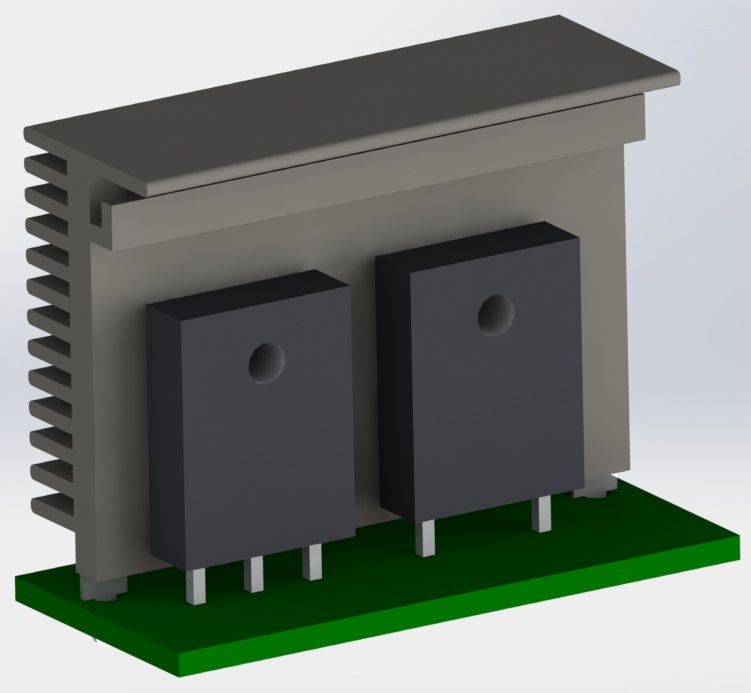
\includegraphics[width=150pt]{Servo_box_model_1.png}
\doxyfigcaption{Energy eater—\+Model 1}
\end{DoxyImage}
  
\item {\bfseries{Model 2}}—for applications with average dissipated power (at 60 degrees C max.) {\bfseries{from 25 W to 120 W (1,000 W peak)}}  
\begin{DoxyImage}
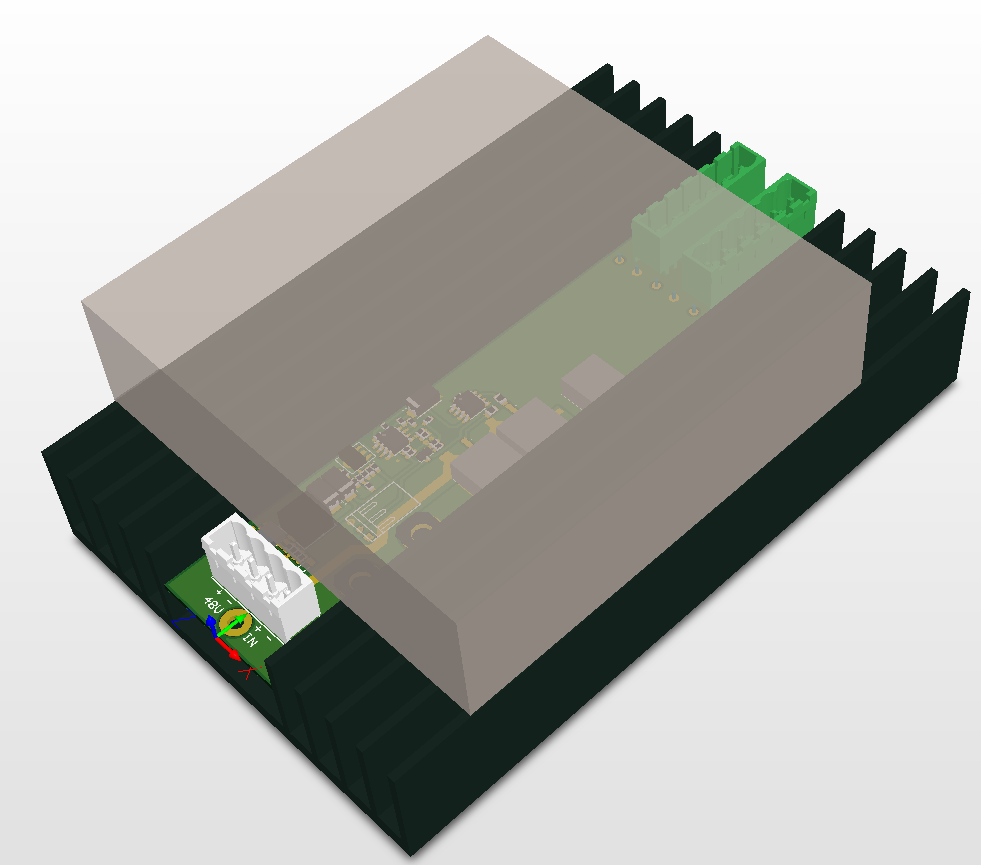
\includegraphics[width=150pt]{eater_isometric.PNG}
\doxyfigcaption{Energy eater—\+Model 2}
\end{DoxyImage}
  
\end{DoxyItemize}

When the average dissipated power of your application is less than 25 W (at 60 degrees C max.), you can also assemble an energy eater on your own based on the schematic below.

 
\begin{DoxyImage}
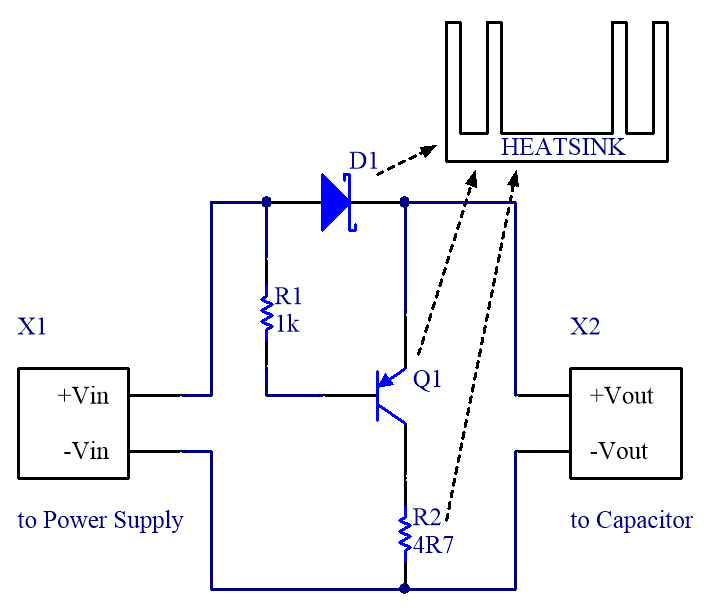
\includegraphics[width=150pt]{eater.png}
\doxyfigcaption{Eater module schematic}
\end{DoxyImage}
 {\bfseries{Required components\+:}} \tabulinesep=1mm
\begin{longtabu}spread 0pt [c]{*{4}{|X[-1]}|}
\hline
\PBS\centering \cellcolor{\tableheadbgcolor}\textbf{ Component   }&\PBS\centering \cellcolor{\tableheadbgcolor}\textbf{ Type   }&\PBS\centering \cellcolor{\tableheadbgcolor}\textbf{ Other options   }&\PBS\centering \cellcolor{\tableheadbgcolor}\textbf{ Comments    }\\\cline{1-4}
\endfirsthead
\hline
\endfoot
\hline
\PBS\centering \cellcolor{\tableheadbgcolor}\textbf{ Component   }&\PBS\centering \cellcolor{\tableheadbgcolor}\textbf{ Type   }&\PBS\centering \cellcolor{\tableheadbgcolor}\textbf{ Other options   }&\PBS\centering \cellcolor{\tableheadbgcolor}\textbf{ Comments    }\\\cline{1-4}
\endhead
D1 -\/ Diode   &APT30\+S20\+BG   &Schottky diode, I\textsubscript{f} {$\ge$} 20 A, V\textsubscript{r} {$\ge$} 96 V   &I\textsubscript{f} {$\ge$} 1.\+5 × Total current of all connected servos    \\\cline{1-4}
Q1 -\/ Transistor   &TIP147   &PNP darlington transistor, V\textsubscript{ce} {$\ge$} 96V, I\textsubscript{c} {$\ge$} 10 A   &\\\cline{1-4}
R1 -\/ Resistor   &1K Ohm, 1 W   &&\\\cline{1-4}
R2 -\/ Resistor   &4.\+7 Ohm, P\textsubscript{d} {$\ge$} 25 W   &&\\\cline{1-4}
X1 -\/ Connector   &&&Input connector (from the power source to the power supply)    \\\cline{1-4}
X2 -\/ Connector   &&&Output connector (from the power consumer to the capacitor and servo)   \\\cline{1-4}
\end{longtabu}


{\bfseries{Heatsink requirements}}~\newline
 

As you can see in the Eater module schematic, D1, Q1, and R2 should be connected to an appropriate heatsink.

Because the energy eater as shown in the schematic dissipates 25 W of average power at the ambient temperature of 60 degrees C max, the heatsink should have thermal resistance of at least 1W/deg C.

To comply with the requirement, select a heatsink with the following characteristics\+: 
\begin{DoxyItemize}
\item forced air convection with the flow rate of 15m3/h 
\item heat dissipating surface of 600 cm2
\end{DoxyItemize}

For example, this can be a heatsink as described below\+: 
\begin{DoxyItemize}
\item heatsink size—100 x 100 mm 
\item fan size—40 x 40 mm 
\item fin quantity—12 
\item fin height—25 mm
\end{DoxyItemize}\hypertarget{group__hw__manual_capacitor}{}\doxysubsubsection{2.\+2 Capacitor module}\label{group__hw__manual_capacitor}
In the servobox solution, capacitors are intended to accumulate electric energy and supply it to servos. The devices allow for compensating short-\/term power consumption peaks that are due to inductive resistance. This is important because inductive resistance values in the servo\textquotesingle{}s power supply circuit are high when the distance from a servo to the supply unit is long. Therefore, the general requirement is to place capacitors as close to servos as possible. For exact distances, refer to Section 3.\+1, Table 1 (\char`\"{}\+L3\char`\"{} column). As part of the servobox solution, capacitor modules are supplied attached to servo motors. However, you can detach them to subsequently mount at admissible distances (see Table 1, \char`\"{}\+L3\char`\"{} column).

 
\begin{DoxyImage}
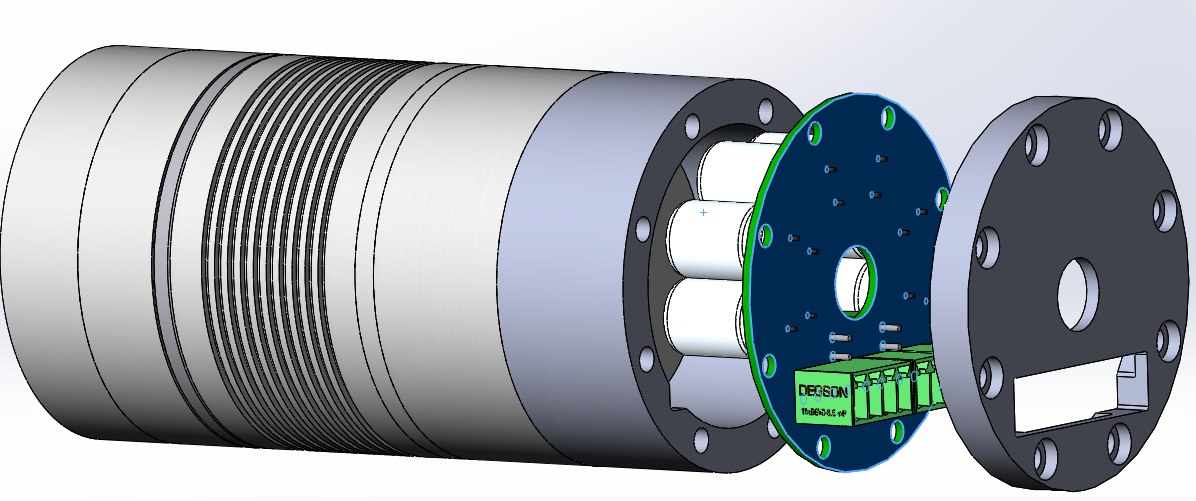
\includegraphics[width=150pt]{Servo_and_capacitor_attached.png}
\doxyfigcaption{An RDrive servo with an attached capacitor module}
\end{DoxyImage}
 

Alternatively, you can assemble a capacitor module on your own, using the schematic below\+:

 
\begin{DoxyImage}
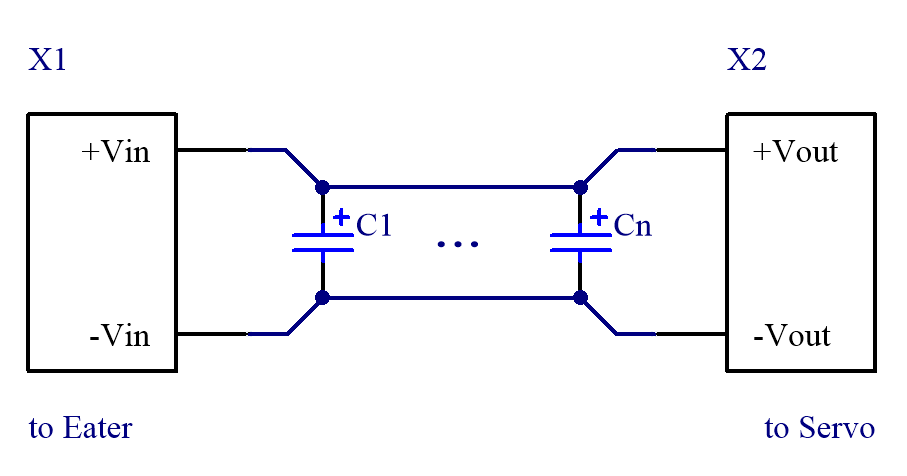
\includegraphics[width=200pt]{capacitor.png}
\doxyfigcaption{Capacitor module schematic}
\end{DoxyImage}
 {\bfseries{Requirements\+:}} \tabulinesep=1mm
\begin{longtabu}spread 0pt [c]{*{3}{|X[-1]}|}
\hline
\PBS\centering \cellcolor{\tableheadbgcolor}\textbf{ Component   }&\PBS\centering \cellcolor{\tableheadbgcolor}\textbf{ Type   }&\PBS\centering \cellcolor{\tableheadbgcolor}\textbf{ Comments    }\\\cline{1-3}
\endfirsthead
\hline
\endfoot
\hline
\PBS\centering \cellcolor{\tableheadbgcolor}\textbf{ Component   }&\PBS\centering \cellcolor{\tableheadbgcolor}\textbf{ Type   }&\PBS\centering \cellcolor{\tableheadbgcolor}\textbf{ Comments    }\\\cline{1-3}
\endhead
X1 -\/ Connector   &&Input connector (power source)    \\\cline{1-3}
X2 -\/ Connector   &&Output connector (from the power consumer to the servo)    \\\cline{1-3}
C1...Cn   &Aluminum electrolytic capacitor or tantalum/polymer capacitor, U {$\ge$} 80 V   &Total capacitance should be {$\ge$} 5 uF per 1 W of connected servo power   \\\cline{1-3}
\end{longtabu}
{\bfseries{Note\+:}} Total capacitor ESR {$\le$} 0.\+1 Ohm\hypertarget{group__hw__manual_sect_conn}{}\doxysubsection{3. Connecting servos to a power supply and a servobox}\label{group__hw__manual_sect_conn}
To integrate an RDrive servo into one circuit with a power supply unit and a servobox, you need to provide the following connections\+:


\begin{DoxyItemize}
\item power supply connection (two wires on the servo housing)
\item CAN communication connection (two wires on the servo housing)
\end{DoxyItemize}

For connection diagrams and requirements, see Sections 3.\+1 and 3.\+2. For eater and capacitor requirements and schematic, see Section 2.\+1 and 2.\+2.\hypertarget{group__hw__manual_sect_21}{}\doxysubsubsection{3.\+1. Power supply connection}\label{group__hw__manual_sect_21}
{\bfseries{Note\+:}} Never supply power before a servo (servos) is (are) fully integrated with a servo box and a power supply unit into one circuit. Charging current of the capacitor(s) can damage the power supply unit or injure the user!

The configuration of the servo box solution (e.\+g., how many eaters and capacitors it uses) and the electrical connection diagram depend on whether your intention is\+:
\begin{DoxyItemize}
\item to connect a single servo, in which case the configuration and the connection diagram are as below\+:  
\begin{DoxyImage}
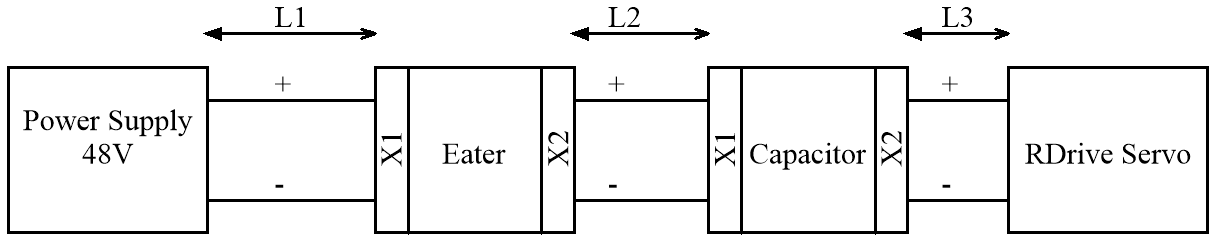
\includegraphics[width=300pt]{single_servo_conn_1.png}
\doxyfigcaption{Connecting single RDrive servo to power supply}
\end{DoxyImage}

\item to connect multiple servos, in which case the configuration and the connection diagram are as below\+:  
\begin{DoxyImage}
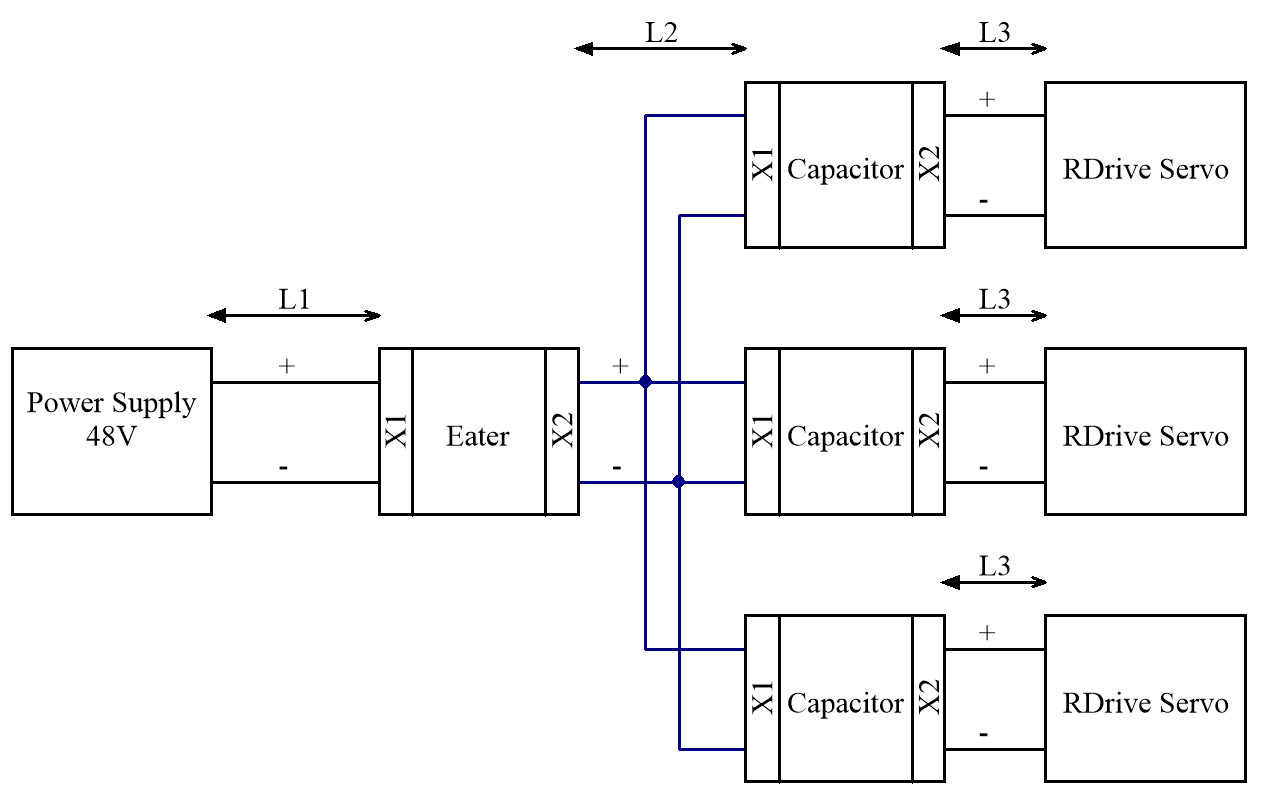
\includegraphics[width=300pt]{multiple_servo_conn_1.png}
\doxyfigcaption{Connecting multiple RDrive servos to power supply}
\end{DoxyImage}

\end{DoxyItemize}

In any case, make sure to meet the following electrical connection requirements\+:
\begin{DoxyItemize}
\item The total circuit length from the power supply unit to any servo motor must not exceed 10 meters.
\item The L1 length must not be longer than 10 meters.
\begin{DoxyItemize}
\item When the total connected motor power is {\bfseries{less than 250 W}}, the cable cross-\/section within the segment must be at least 1.\+00 mm2.
\item When the total connected motor power is {\bfseries{less than 500 W}}, the cable cross-\/section within the segment must be at least 2.\+00 mm2.
\end{DoxyItemize}
\item The L2 length (from the eater to the capacitor) must not exceed the values from Table 1.
\item The L3 length (from the capacitor to any servo) must not exceed the values from Table 1.
\end{DoxyItemize}

{\bfseries{Table 1\+: Line segment lengths vs. cross-\/sections}} \tabulinesep=1mm
\begin{longtabu}spread 0pt [c]{*{15}{|X[-1]}|}
\hline
\PBS\centering \cellcolor{\tableheadbgcolor}\textbf{ Servo model   }&\multicolumn{6}{c|}{\PBS\centering \cellcolor{\tableheadbgcolor}\textbf{ L2   }}&\multicolumn{8}{c|}{\PBS\centering \cellcolor{\tableheadbgcolor}\textbf{ L3    }}\\\cline{1-15}
\endfirsthead
\hline
\endfoot
\hline
\PBS\centering \cellcolor{\tableheadbgcolor}\textbf{ Servo model   }&\multicolumn{6}{c|}{\PBS\centering \cellcolor{\tableheadbgcolor}\textbf{ L2   }}&\multicolumn{8}{c|}{\PBS\centering \cellcolor{\tableheadbgcolor}\textbf{ L3    }}\\\cline{1-15}
\endhead
&0.\+75 mm\textsuperscript{2}   &1.\+0 mm\textsuperscript{2}   &1.\+5 mm\textsuperscript{2}   &2.\+5 mm\textsuperscript{2}   &4.\+0 mm\textsuperscript{2}   &6.\+0 mm\textsuperscript{2}   &0.\+25 mm\textsuperscript{2}   &0.\+5 mm\textsuperscript{2}   &0.\+75 mm\textsuperscript{2}   &1.\+0 mm\textsuperscript{2}   &1.\+5 mm\textsuperscript{2}   &2.\+5 mm\textsuperscript{2}   &4.\+0 mm\textsuperscript{2}   &6.\+0 mm\textsuperscript{2}    \\\cline{1-15}
RD50   &4 m   &5 m   &8 m   &10 m   &10 m   &10 m   &0.\+1 m   &0.\+1 m   &0.\+2 m   &0.\+2 m   &0.\+4 m   &0.\+7 m   &1.\+0 m   &1.\+0 m    \\\cline{1-15}
RD60   &2 m   &3 m   &5 m   &9 m   &10 m   &10 m   &-\/   &0.\+1 m   &0.\+1 m   &0.\+1 m   &0.\+2 m   &0.\+4 m   &1.\+0 m   &1.\+0 m    \\\cline{1-15}
RD85   &0.\+8 m   &1 m   &1 m   &2 m   &4 m   &6 m   &-\/   &-\/   &-\/   &-\/   &0.\+08 m   &0.\+13 m   &0.\+21 m   &0.\+32 m   \\\cline{1-15}
\end{longtabu}
\hypertarget{group__hw__manual_sect_22}{}\doxysubsubsection{3.\+2. CAN connection}\label{group__hw__manual_sect_22}
The CAN connection of RDrive servos is a two-\/wire bus line transmitting differential signals\+: CAN\+\_\+\+HIGH and CAN\+\_\+\+LOW. The configuration of the bus line is as illustrated below\+:  
\begin{DoxyImage}
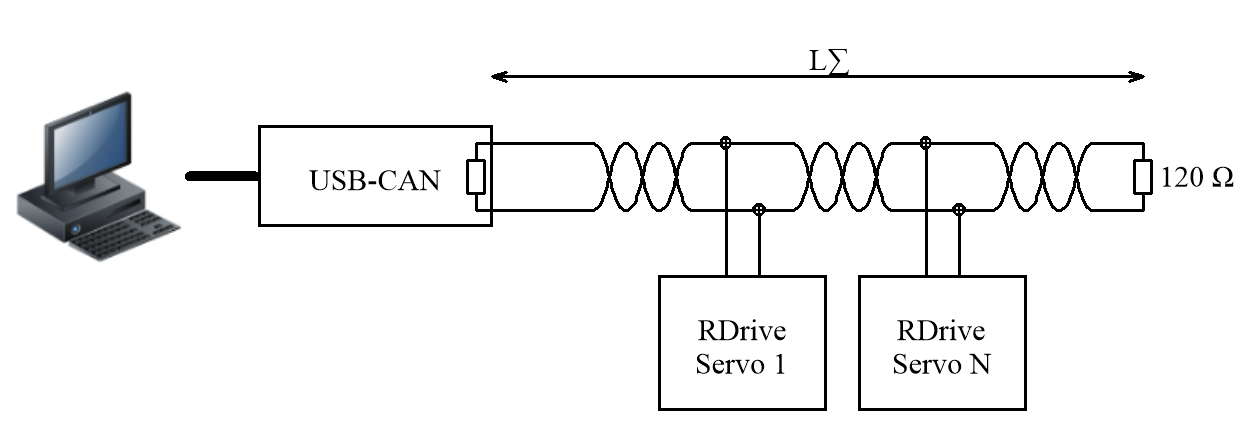
\includegraphics[width=300pt]{servobox_CAN_new_1.png}
\doxyfigcaption{Connecting RDrive servos to USB-\/\+CAN}
\end{DoxyImage}


Providing the CAN connection, make sure to comply with the following requirements\+:
\begin{DoxyItemize}
\item CAN bus lines of less than 40 m long should be terminated with 120 Ohm resistors at both ends. For bus lines of over 40 m long, use 150-\/300 Ohm resistors.~\newline
 {\bfseries{Note\+:}} You have to provide only one resistor because one is already integrated into the CAN-\/\+USB dongle supplied as part of the servobox solution.
\item The bus line cable must be a twisted pair cable with the lay length of 2 to 4 cm.
\item For the cross section of the bus line, see Table 2.
\item To ensure the baud rate required for your application, L{$\Sigma$} should meet the specific values as indicated in Table 2.
\end{DoxyItemize}

{\bfseries{Table 2\+: CAN line parameters}} \tabulinesep=1mm
\begin{longtabu}spread 0pt [c]{*{6}{|X[-1]}|}
\hline
\PBS\centering \cellcolor{\tableheadbgcolor}\textbf{ Baud Rate   }&\PBS\centering \cellcolor{\tableheadbgcolor}\textbf{ 50 kbit/s   }&\PBS\centering \cellcolor{\tableheadbgcolor}\textbf{ 100 kbit/s   }&\PBS\centering \cellcolor{\tableheadbgcolor}\textbf{ 250 kbit/s   }&\PBS\centering \cellcolor{\tableheadbgcolor}\textbf{ 500 kbit/s   }&\PBS\centering \cellcolor{\tableheadbgcolor}\textbf{ 1 Mbit/s    }\\\cline{1-6}
\endfirsthead
\hline
\endfoot
\hline
\PBS\centering \cellcolor{\tableheadbgcolor}\textbf{ Baud Rate   }&\PBS\centering \cellcolor{\tableheadbgcolor}\textbf{ 50 kbit/s   }&\PBS\centering \cellcolor{\tableheadbgcolor}\textbf{ 100 kbit/s   }&\PBS\centering \cellcolor{\tableheadbgcolor}\textbf{ 250 kbit/s   }&\PBS\centering \cellcolor{\tableheadbgcolor}\textbf{ 500 kbit/s   }&\PBS\centering \cellcolor{\tableheadbgcolor}\textbf{ 1 Mbit/s    }\\\cline{1-6}
\endhead
Total line length, L{$\Sigma$}, m   &$<$ 1000   &$<$ 500   &$<$ 200   &$<$ 100   &$<$ 40    \\\cline{1-6}
Cross-\/section, mm2   &0.\+75 to 0.\+8   &0.\+5 to 0.\+6   &0.\+34 to 0.\+6   &0.\+34 to 0.\+6   &0.\+25 to 0.\+34   \\\cline{1-6}
\end{longtabu}


{\bfseries{Connecting multiple servos to a CAN bus}}

To avoid collisions, each servo connected to a CAN bus line must have a unique CAN identifier. However, RDrive servo motors are all supplied with the same {\bfseries{default ID—32}}. Therefore, an important step of connecting multiple RDrive servos to a single CAN bus line is to change their default IDs to unique ones.

Start with connecting each of your multiple servos, one by one, to a CAN bus line, following the sequence as described below\+:~\newline


{\bfseries{Caution!}} Never connect or disconnect servos when power supply is on!~\newline



\begin{DoxyEnumerate}
\item Take servo 1 and connect it to the CAN bus line as desribed in this section above.~\newline

\item Run the \mbox{\hyperlink{group__tutor__c__change_i_d1}{Changing CAN ID of a single servo}} tutorial to change the servo\textquotesingle{}s default ID.~\newline

\item Remember or write down the newly assigned CAN ID and disconnect the servo.~\newline

\item Repeat Steps 1 to 3 for all the servos you want to connect to the same CAN bus line.~\newline

\end{DoxyEnumerate}

Once you have changed all CAN IDs as appropriate, you can connect all the servos back to the CAN bus line and start working with them.

{\bfseries{Note}}\+: In total, you can connect up to 127 devices to a single CAN bus. So, the admissible CAN ID pool is from 1 to 127. 
\hypertarget{group__tutor__c__servomove1}{}\doxysection{PVT trajectory for one servo}
\label{group__tutor__c__servomove1}\index{PVT trajectory for one servo@{PVT trajectory for one servo}}
The tutorial describes how to set up and execute a motion trajectory for one servo. In this example, the motion trajectory comprises two PVT (position-\/velocity-\/time) points\+: 
\begin{DoxyItemize}
\item one PVT commanding the servo to move to the position of 100 degrees in 6,000 milliseconds 
\item one PVT commanding the servo to move to the position of -\/100 degrees in 6,000 milliseconds
\end{DoxyItemize}


\begin{DoxyEnumerate}
\item Initialize the interface. 
\begin{DoxyCodeInclude}{0}
\DoxyCodeLine{    \mbox{\hyperlink{structrr__can__interface__t}{rr\_can\_interface\_t}} *iface = \mbox{\hyperlink{group___init_ga472a4890dcc7d7a13123c56a06946d91}{rr\_init\_interface}}(argv[1]);}
\DoxyCodeLine{    \textcolor{keywordflow}{if}(!iface)}
\DoxyCodeLine{    \{}
\DoxyCodeLine{        \mbox{\hyperlink{api_8h_a0e4aafa2ca9bd25219713176906b7c40}{API\_DEBUG}}(\textcolor{stringliteral}{"{}Interface init error\(\backslash\)n"{}});}
\DoxyCodeLine{        \textcolor{keywordflow}{return} 1;}
\DoxyCodeLine{    \}}

\end{DoxyCodeInclude}

\item Initialize the servo. 
\begin{DoxyCodeInclude}{0}
\DoxyCodeLine{    \mbox{\hyperlink{structrr__servo__t}{rr\_servo\_t}} *servo = \mbox{\hyperlink{group___init_ga88467da814964fd147ab9c7c7af0ed21}{rr\_init\_servo}}(iface, \textcolor{keywordtype}{id});}
\DoxyCodeLine{    \textcolor{keywordflow}{if}(!servo)}
\DoxyCodeLine{    \{}
\DoxyCodeLine{        \mbox{\hyperlink{api_8h_a0e4aafa2ca9bd25219713176906b7c40}{API\_DEBUG}}(\textcolor{stringliteral}{"{}Servo init error\(\backslash\)n"{}});}
\DoxyCodeLine{        \textcolor{keywordflow}{return} 1;}
\DoxyCodeLine{    \}}

\end{DoxyCodeInclude}

\item Clear the motion queue. 
\begin{DoxyCodeInclude}{0}
\DoxyCodeLine{    \mbox{\hyperlink{group___trajectory_ga7b5be2d97da325eefde671c2e65e8055}{rr\_clear\_points\_all}}(servo);}

\end{DoxyCodeInclude}
 {\bfseries{ Adding PVT points to form a motion queue }}
\item Set the first PVT point, commanding the servo to move to the position of 100 degrees in 6,000 milliseconds. {\bfseries{Note}}\+: When a point is added successfully to the motion queue, the function will return OK. Otherwise, the function returns an error warning and quits the program. 
\begin{DoxyCodeInclude}{0}
\DoxyCodeLine{    \textcolor{keywordtype}{int} status = \mbox{\hyperlink{group___trajectory_gacf26f2966a4f2035a128e1fcecd08f58}{rr\_add\_motion\_point}}(servo, 100.0, 0.0, 6000);}
\DoxyCodeLine{    \textcolor{keywordflow}{if}(status != \mbox{\hyperlink{api_8h_a92d5be5038abcf89837faf85a08debdca4894234446e2d92068943b3d6d3a0bdc}{RET\_OK}})}
\DoxyCodeLine{    \{}
\DoxyCodeLine{        \mbox{\hyperlink{api_8h_a0e4aafa2ca9bd25219713176906b7c40}{API\_DEBUG}}(\textcolor{stringliteral}{"{}Error in the trjectory point calculation: \%d\(\backslash\)n"{}}, status);}
\DoxyCodeLine{        \textcolor{keywordflow}{return} 1;}
\DoxyCodeLine{    \}}

\end{DoxyCodeInclude}

\item Set the second PVT point, commanding the servo to move to the position of -\/100 degrees in 6,000 milliseconds. {\bfseries{Note}}\+: When a point is added successfully to the motion queue, the function will return OK. Otherwise, the function returns an error warning and quits the program. 
\begin{DoxyCodeInclude}{0}
\DoxyCodeLine{    status = \mbox{\hyperlink{group___trajectory_gacf26f2966a4f2035a128e1fcecd08f58}{rr\_add\_motion\_point}}(servo, -\/100.0, 0.0, 6000);}
\DoxyCodeLine{    \textcolor{keywordflow}{if}(status != \mbox{\hyperlink{api_8h_a92d5be5038abcf89837faf85a08debdca4894234446e2d92068943b3d6d3a0bdc}{RET\_OK}})}
\DoxyCodeLine{    \{}
\DoxyCodeLine{        \mbox{\hyperlink{api_8h_a0e4aafa2ca9bd25219713176906b7c40}{API\_DEBUG}}(\textcolor{stringliteral}{"{}Error in the trjectory point calculation: \%d\(\backslash\)n"{}}, status);}
\DoxyCodeLine{        \textcolor{keywordflow}{return} 1;}
\DoxyCodeLine{    \}}

\end{DoxyCodeInclude}
 {\bfseries{ Executing the resulting motion queue }}
\item Command the servo to move through the PVT points you added to the motion queue. Set the function parameter to 0 to get the servo moving without a delay. 
\begin{DoxyCodeInclude}{0}
\DoxyCodeLine{    \mbox{\hyperlink{group___trajectory_ga639ef9f16dd649cbedfd65daca35ee18}{rr\_start\_motion}}(iface, 0);}

\end{DoxyCodeInclude}

\item To ensure the program will not move on to execute another operation, set an idle period of 14,000 milliseconds. 
\begin{DoxyCodeInclude}{0}
\DoxyCodeLine{    \mbox{\hyperlink{group___aux_gaeb26028b83635e028ebc901e1cbf33a1}{rr\_sleep\_ms}}(14000); \textcolor{comment}{// wait till the movement ends}}

\end{DoxyCodeInclude}
 {\bfseries{ Complete tutorial code\+: }} 
\begin{DoxyCodeInclude}{0}
\DoxyCodeLine{    \mbox{\hyperlink{structrr__can__interface__t}{rr\_can\_interface\_t}} *iface = \mbox{\hyperlink{group___init_ga472a4890dcc7d7a13123c56a06946d91}{rr\_init\_interface}}(argv[1]);}
\DoxyCodeLine{    \textcolor{keywordflow}{if}(!iface)}
\DoxyCodeLine{    \{}
\DoxyCodeLine{        \mbox{\hyperlink{api_8h_a0e4aafa2ca9bd25219713176906b7c40}{API\_DEBUG}}(\textcolor{stringliteral}{"{}Interface init error\(\backslash\)n"{}});}
\DoxyCodeLine{        \textcolor{keywordflow}{return} 1;}
\DoxyCodeLine{    \}}
\DoxyCodeLine{}
\DoxyCodeLine{    \mbox{\hyperlink{structrr__servo__t}{rr\_servo\_t}} *servo = \mbox{\hyperlink{group___init_ga88467da814964fd147ab9c7c7af0ed21}{rr\_init\_servo}}(iface, \textcolor{keywordtype}{id});}
\DoxyCodeLine{    \textcolor{keywordflow}{if}(!servo)}
\DoxyCodeLine{    \{}
\DoxyCodeLine{        \mbox{\hyperlink{api_8h_a0e4aafa2ca9bd25219713176906b7c40}{API\_DEBUG}}(\textcolor{stringliteral}{"{}Servo init error\(\backslash\)n"{}});}
\DoxyCodeLine{        \textcolor{keywordflow}{return} 1;}
\DoxyCodeLine{    \}}
\DoxyCodeLine{}
\DoxyCodeLine{    \mbox{\hyperlink{group___state_ga0b1d17a317892471c6df1440e92da9d8}{rr\_servo\_set\_state\_operational}}(servo);}
\DoxyCodeLine{}
\DoxyCodeLine{    \mbox{\hyperlink{api_8h_a0e4aafa2ca9bd25219713176906b7c40}{API\_DEBUG}}(\textcolor{stringliteral}{"{}========== Tutorial of the \%s ==========\(\backslash\)n"{}}, \textcolor{stringliteral}{"{}controlling one servo"{}});}
\DoxyCodeLine{}
\DoxyCodeLine{    \mbox{\hyperlink{group___trajectory_ga7b5be2d97da325eefde671c2e65e8055}{rr\_clear\_points\_all}}(servo);}
\DoxyCodeLine{    \mbox{\hyperlink{api_8h_a0e4aafa2ca9bd25219713176906b7c40}{API\_DEBUG}}(\textcolor{stringliteral}{"{}Appending points\(\backslash\)n"{}});}
\DoxyCodeLine{    \textcolor{keywordtype}{int} status = \mbox{\hyperlink{group___trajectory_gacf26f2966a4f2035a128e1fcecd08f58}{rr\_add\_motion\_point}}(servo, 100.0, 0.0, 6000);}
\DoxyCodeLine{    \textcolor{keywordflow}{if}(status != \mbox{\hyperlink{api_8h_a92d5be5038abcf89837faf85a08debdca4894234446e2d92068943b3d6d3a0bdc}{RET\_OK}})}
\DoxyCodeLine{    \{}
\DoxyCodeLine{        \mbox{\hyperlink{api_8h_a0e4aafa2ca9bd25219713176906b7c40}{API\_DEBUG}}(\textcolor{stringliteral}{"{}Error in the trjectory point calculation: \%d\(\backslash\)n"{}}, status);}
\DoxyCodeLine{        \textcolor{keywordflow}{return} 1;}
\DoxyCodeLine{    \}}
\DoxyCodeLine{    status = \mbox{\hyperlink{group___trajectory_gacf26f2966a4f2035a128e1fcecd08f58}{rr\_add\_motion\_point}}(servo, -\/100.0, 0.0, 6000);}
\DoxyCodeLine{    \textcolor{keywordflow}{if}(status != \mbox{\hyperlink{api_8h_a92d5be5038abcf89837faf85a08debdca4894234446e2d92068943b3d6d3a0bdc}{RET\_OK}})}
\DoxyCodeLine{    \{}
\DoxyCodeLine{        \mbox{\hyperlink{api_8h_a0e4aafa2ca9bd25219713176906b7c40}{API\_DEBUG}}(\textcolor{stringliteral}{"{}Error in the trjectory point calculation: \%d\(\backslash\)n"{}}, status);}
\DoxyCodeLine{        \textcolor{keywordflow}{return} 1;}
\DoxyCodeLine{    \}}
\DoxyCodeLine{    \mbox{\hyperlink{group___trajectory_ga639ef9f16dd649cbedfd65daca35ee18}{rr\_start\_motion}}(iface, 0);}
\DoxyCodeLine{    \mbox{\hyperlink{group___aux_gaeb26028b83635e028ebc901e1cbf33a1}{rr\_sleep\_ms}}(14000); \textcolor{comment}{// wait till the movement ends}}

\end{DoxyCodeInclude}

\end{DoxyEnumerate}
\hypertarget{group__tutor__c__servomove2}{}\doxysection{PVT trajectory for two servos}
\label{group__tutor__c__servomove2}\index{PVT trajectory for two servos@{PVT trajectory for two servos}}
The tutorial describes how to set up motion trajectories for two servos and to execute them simultaneously. In this example, each motion trajectory comprises two PVT (position-\/velocity-\/time) points\+: 
\begin{DoxyItemize}
\item one PVT commanding servos to move to the position of 100 degrees in 6,000 milliseconds 
\item one PVT commanding servos to move to the position of -\/100 degrees in 6,000 milliseconds
\end{DoxyItemize}

{\bfseries{Important!}}Before setting up PVT points, make sure to change the default CAN ID of at least one of the servos (see the \mbox{\hyperlink{group__tutor__c__change_i_d1}{Changing CAN ID of a single servo}} tutorial).

{\bfseries{Note\+:}} When you set a PVT trajectory to move more than one servo simultaneously, mind that the clock rate of the servos can differ by up to 2-\/3\%. Therefore, if the preset PVT trajectory is rather long, servos can get desynchronized. To avoid the desynchronization, we have implemented the following mechanism\+: 
\begin{DoxyItemize}
\item The device controlling the servos broadcasts a sync CAN frame to all servos on an interface. The frame should have the following format\+:~\newline
 ID = 0x27f, data = uint32 (4 bytes),~\newline
 {\bfseries{Where\+:}} ‘data’ stands for the microseconds counter value by modulus of 600,000,000, starting from any value. 
\item Servos receive the frame and try to adjust their clock rates to that of the device using the PLL. The adjustment proper starts after the servos receive the second frame and can take up to 5 seconds, depending on the broadcasting frequency. The higher the broadcasting frequency, the less time the adjustment takes. 
\item The broadcasting frequency is 5 Hz minimum. The recommended frequency range is from 10 to 20 Hz. When the sync frames are not broadcast or the broadcast frequency is below 5 Hz, the clock rate of servos is as usual.


\begin{DoxyEnumerate}
\item Initialize the interface. 
\begin{DoxyCodeInclude}{0}
\DoxyCodeLine{    \mbox{\hyperlink{structrr__can__interface__t}{rr\_can\_interface\_t}} *iface = \mbox{\hyperlink{group___init_ga472a4890dcc7d7a13123c56a06946d91}{rr\_init\_interface}}(argv[1]);}
\DoxyCodeLine{    \textcolor{keywordflow}{if}(!iface)}
\DoxyCodeLine{    \{}
\DoxyCodeLine{        \mbox{\hyperlink{api_8h_a0e4aafa2ca9bd25219713176906b7c40}{API\_DEBUG}}(\textcolor{stringliteral}{"{}Interface init error\(\backslash\)n"{}});}
\DoxyCodeLine{        \textcolor{keywordflow}{return} 1;}
\DoxyCodeLine{    \}}

\end{DoxyCodeInclude}

\item Initialize servo 1. 
\begin{DoxyCodeInclude}{0}
\DoxyCodeLine{    \mbox{\hyperlink{structrr__servo__t}{rr\_servo\_t}} *servo1 = \mbox{\hyperlink{group___init_ga88467da814964fd147ab9c7c7af0ed21}{rr\_init\_servo}}(iface, id1);}
\DoxyCodeLine{    \textcolor{keywordflow}{if}(!servo1)}
\DoxyCodeLine{    \{}
\DoxyCodeLine{        \mbox{\hyperlink{api_8h_a0e4aafa2ca9bd25219713176906b7c40}{API\_DEBUG}}(\textcolor{stringliteral}{"{}Servo \#1 init error\(\backslash\)n"{}});}
\DoxyCodeLine{        \textcolor{keywordflow}{return} 1;}
\DoxyCodeLine{    \}}

\end{DoxyCodeInclude}

\item Initialize servo 2. 
\begin{DoxyCodeInclude}{0}
\DoxyCodeLine{    \mbox{\hyperlink{structrr__servo__t}{rr\_servo\_t}} *servo2 = \mbox{\hyperlink{group___init_ga88467da814964fd147ab9c7c7af0ed21}{rr\_init\_servo}}(iface, id2);}
\DoxyCodeLine{    \textcolor{keywordflow}{if}(!servo2)}
\DoxyCodeLine{    \{}
\DoxyCodeLine{        \mbox{\hyperlink{api_8h_a0e4aafa2ca9bd25219713176906b7c40}{API\_DEBUG}}(\textcolor{stringliteral}{"{}Servo \#2 init error\(\backslash\)n"{}});}
\DoxyCodeLine{        \textcolor{keywordflow}{return} 1;}
\DoxyCodeLine{    \}}

\end{DoxyCodeInclude}

\item Clear the motion queue of servo 1. 
\begin{DoxyCodeInclude}{0}
\DoxyCodeLine{    \mbox{\hyperlink{group___trajectory_ga7b5be2d97da325eefde671c2e65e8055}{rr\_clear\_points\_all}}(servo1);}

\end{DoxyCodeInclude}

\item Clear the motion queue of servo 2. 
\begin{DoxyCodeInclude}{0}
\DoxyCodeLine{    \mbox{\hyperlink{group___trajectory_ga7b5be2d97da325eefde671c2e65e8055}{rr\_clear\_points\_all}}(servo2);}

\end{DoxyCodeInclude}
 {\bfseries{ Adding PVT points to form motion queues}}
\item Set the first PVT point for servo 1, commanding it to move to the position of 100 degrees in 6,000 milliseconds. 
\begin{DoxyCodeInclude}{0}
\DoxyCodeLine{    \textcolor{keywordtype}{int} status = \mbox{\hyperlink{group___trajectory_gacf26f2966a4f2035a128e1fcecd08f58}{rr\_add\_motion\_point}}(servo1, 100.0, 0.0, 6000);}
\DoxyCodeLine{    \textcolor{keywordflow}{if}(status != \mbox{\hyperlink{api_8h_a92d5be5038abcf89837faf85a08debdca4894234446e2d92068943b3d6d3a0bdc}{RET\_OK}})}
\DoxyCodeLine{    \{}
\DoxyCodeLine{        \mbox{\hyperlink{api_8h_a0e4aafa2ca9bd25219713176906b7c40}{API\_DEBUG}}(\textcolor{stringliteral}{"{}Error in the trjectory point calculation: \%d\(\backslash\)n"{}}, status);}
\DoxyCodeLine{        \textcolor{keywordflow}{return} 1;}
\DoxyCodeLine{    \}}

\end{DoxyCodeInclude}

\item Set the first PVT point for servo 2, commanding it to move to the position of 100 degrees in 6,000 milliseconds. 
\begin{DoxyCodeInclude}{0}
\DoxyCodeLine{    status = \mbox{\hyperlink{group___trajectory_gacf26f2966a4f2035a128e1fcecd08f58}{rr\_add\_motion\_point}}(servo2, 100.0, 0.0, 6000);}
\DoxyCodeLine{    \textcolor{keywordflow}{if}(status != \mbox{\hyperlink{api_8h_a92d5be5038abcf89837faf85a08debdca4894234446e2d92068943b3d6d3a0bdc}{RET\_OK}})}
\DoxyCodeLine{    \{}
\DoxyCodeLine{        \mbox{\hyperlink{api_8h_a0e4aafa2ca9bd25219713176906b7c40}{API\_DEBUG}}(\textcolor{stringliteral}{"{}Error in the trjectory point calculation: \%d\(\backslash\)n"{}}, status);}
\DoxyCodeLine{        \textcolor{keywordflow}{return} 1;}
\DoxyCodeLine{    \}}

\end{DoxyCodeInclude}

\item Set the second PVT point for servo 1, commanding it to move to the position of -\/100 degrees in 6,000 milliseconds. 
\begin{DoxyCodeInclude}{0}
\DoxyCodeLine{    status = \mbox{\hyperlink{group___trajectory_gacf26f2966a4f2035a128e1fcecd08f58}{rr\_add\_motion\_point}}(servo1, -\/100.0, 0.0, 6000);}
\DoxyCodeLine{    \textcolor{keywordflow}{if}(status != \mbox{\hyperlink{api_8h_a92d5be5038abcf89837faf85a08debdca4894234446e2d92068943b3d6d3a0bdc}{RET\_OK}})}
\DoxyCodeLine{    \{}
\DoxyCodeLine{        \mbox{\hyperlink{api_8h_a0e4aafa2ca9bd25219713176906b7c40}{API\_DEBUG}}(\textcolor{stringliteral}{"{}Error in the trjectory point calculation: \%d\(\backslash\)n"{}}, status);}
\DoxyCodeLine{        \textcolor{keywordflow}{return} 1;}
\DoxyCodeLine{    \}}

\end{DoxyCodeInclude}

\item Set the second PVT point for servo 2, commanding it to move to the position of -\/100 degrees in 6,000 milliseconds. 
\begin{DoxyCodeInclude}{0}
\DoxyCodeLine{    status = \mbox{\hyperlink{group___trajectory_gacf26f2966a4f2035a128e1fcecd08f58}{rr\_add\_motion\_point}}(servo2, -\/100.0, 0.0, 6000);}
\DoxyCodeLine{    \textcolor{keywordflow}{if}(status != \mbox{\hyperlink{api_8h_a92d5be5038abcf89837faf85a08debdca4894234446e2d92068943b3d6d3a0bdc}{RET\_OK}})}
\DoxyCodeLine{    \{}
\DoxyCodeLine{        \mbox{\hyperlink{api_8h_a0e4aafa2ca9bd25219713176906b7c40}{API\_DEBUG}}(\textcolor{stringliteral}{"{}Error in the trjectory point calculation: \%d\(\backslash\)n"{}}, status);}
\DoxyCodeLine{        \textcolor{keywordflow}{return} 1;}
\DoxyCodeLine{    \}}

\end{DoxyCodeInclude}
 {\bfseries{ Executing the resulting motion queues}}
\item Command all servos to move simultaneously. Each of the two servos will execute their preset motion queues. Set the function parameter to 0 to get the servos moving without a delay. 
\begin{DoxyCodeInclude}{0}
\DoxyCodeLine{    \mbox{\hyperlink{group___trajectory_ga639ef9f16dd649cbedfd65daca35ee18}{rr\_start\_motion}}(iface, 0);}

\end{DoxyCodeInclude}

\item To ensure the program will not move on to execute another operation, set an idle period of 14,000 milliseconds. 
\begin{DoxyCodeInclude}{0}
\DoxyCodeLine{    \mbox{\hyperlink{group___aux_gaeb26028b83635e028ebc901e1cbf33a1}{rr\_sleep\_ms}}(14000); \textcolor{comment}{//wait till the movement ends}}

\end{DoxyCodeInclude}
 {\bfseries{ Complete tutorial code\+: }} 
\begin{DoxyCodeInclude}{0}
\DoxyCodeLine{    \mbox{\hyperlink{structrr__can__interface__t}{rr\_can\_interface\_t}} *iface = \mbox{\hyperlink{group___init_ga472a4890dcc7d7a13123c56a06946d91}{rr\_init\_interface}}(argv[1]);}
\DoxyCodeLine{    \textcolor{keywordflow}{if}(!iface)}
\DoxyCodeLine{    \{}
\DoxyCodeLine{        \mbox{\hyperlink{api_8h_a0e4aafa2ca9bd25219713176906b7c40}{API\_DEBUG}}(\textcolor{stringliteral}{"{}Interface init error\(\backslash\)n"{}});}
\DoxyCodeLine{        \textcolor{keywordflow}{return} 1;}
\DoxyCodeLine{    \}}
\DoxyCodeLine{    \mbox{\hyperlink{structrr__servo__t}{rr\_servo\_t}} *servo1 = \mbox{\hyperlink{group___init_ga88467da814964fd147ab9c7c7af0ed21}{rr\_init\_servo}}(iface, id1);}
\DoxyCodeLine{    \textcolor{keywordflow}{if}(!servo1)}
\DoxyCodeLine{    \{}
\DoxyCodeLine{        \mbox{\hyperlink{api_8h_a0e4aafa2ca9bd25219713176906b7c40}{API\_DEBUG}}(\textcolor{stringliteral}{"{}Servo \#1 init error\(\backslash\)n"{}});}
\DoxyCodeLine{        \textcolor{keywordflow}{return} 1;}
\DoxyCodeLine{    \}}
\DoxyCodeLine{    \mbox{\hyperlink{structrr__servo__t}{rr\_servo\_t}} *servo2 = \mbox{\hyperlink{group___init_ga88467da814964fd147ab9c7c7af0ed21}{rr\_init\_servo}}(iface, id2);}
\DoxyCodeLine{    \textcolor{keywordflow}{if}(!servo2)}
\DoxyCodeLine{    \{}
\DoxyCodeLine{        \mbox{\hyperlink{api_8h_a0e4aafa2ca9bd25219713176906b7c40}{API\_DEBUG}}(\textcolor{stringliteral}{"{}Servo \#2 init error\(\backslash\)n"{}});}
\DoxyCodeLine{        \textcolor{keywordflow}{return} 1;}
\DoxyCodeLine{    \}}
\DoxyCodeLine{}
\DoxyCodeLine{    \mbox{\hyperlink{group___state_ga0b1d17a317892471c6df1440e92da9d8}{rr\_servo\_set\_state\_operational}}(servo1);}
\DoxyCodeLine{    \mbox{\hyperlink{group___state_ga0b1d17a317892471c6df1440e92da9d8}{rr\_servo\_set\_state\_operational}}(servo2);}
\DoxyCodeLine{}
\DoxyCodeLine{    \mbox{\hyperlink{api_8h_a0e4aafa2ca9bd25219713176906b7c40}{API\_DEBUG}}(\textcolor{stringliteral}{"{}========== Tutorial of the \%s ==========\(\backslash\)n"{}}, \textcolor{stringliteral}{"{}controlling two servos"{}});}
\DoxyCodeLine{}
\DoxyCodeLine{    \mbox{\hyperlink{group___trajectory_ga7b5be2d97da325eefde671c2e65e8055}{rr\_clear\_points\_all}}(servo1);}
\DoxyCodeLine{    \mbox{\hyperlink{group___trajectory_ga7b5be2d97da325eefde671c2e65e8055}{rr\_clear\_points\_all}}(servo2);}
\DoxyCodeLine{}
\DoxyCodeLine{    \textcolor{keywordtype}{int} status = \mbox{\hyperlink{group___trajectory_gacf26f2966a4f2035a128e1fcecd08f58}{rr\_add\_motion\_point}}(servo1, 100.0, 0.0, 6000);}
\DoxyCodeLine{    \textcolor{keywordflow}{if}(status != \mbox{\hyperlink{api_8h_a92d5be5038abcf89837faf85a08debdca4894234446e2d92068943b3d6d3a0bdc}{RET\_OK}})}
\DoxyCodeLine{    \{}
\DoxyCodeLine{        \mbox{\hyperlink{api_8h_a0e4aafa2ca9bd25219713176906b7c40}{API\_DEBUG}}(\textcolor{stringliteral}{"{}Error in the trjectory point calculation: \%d\(\backslash\)n"{}}, status);}
\DoxyCodeLine{        \textcolor{keywordflow}{return} 1;}
\DoxyCodeLine{    \}}
\DoxyCodeLine{    status = \mbox{\hyperlink{group___trajectory_gacf26f2966a4f2035a128e1fcecd08f58}{rr\_add\_motion\_point}}(servo2, 100.0, 0.0, 6000);}
\DoxyCodeLine{    \textcolor{keywordflow}{if}(status != \mbox{\hyperlink{api_8h_a92d5be5038abcf89837faf85a08debdca4894234446e2d92068943b3d6d3a0bdc}{RET\_OK}})}
\DoxyCodeLine{    \{}
\DoxyCodeLine{        \mbox{\hyperlink{api_8h_a0e4aafa2ca9bd25219713176906b7c40}{API\_DEBUG}}(\textcolor{stringliteral}{"{}Error in the trjectory point calculation: \%d\(\backslash\)n"{}}, status);}
\DoxyCodeLine{        \textcolor{keywordflow}{return} 1;}
\DoxyCodeLine{    \}}
\DoxyCodeLine{    status = \mbox{\hyperlink{group___trajectory_gacf26f2966a4f2035a128e1fcecd08f58}{rr\_add\_motion\_point}}(servo1, -\/100.0, 0.0, 6000);}
\DoxyCodeLine{    \textcolor{keywordflow}{if}(status != \mbox{\hyperlink{api_8h_a92d5be5038abcf89837faf85a08debdca4894234446e2d92068943b3d6d3a0bdc}{RET\_OK}})}
\DoxyCodeLine{    \{}
\DoxyCodeLine{        \mbox{\hyperlink{api_8h_a0e4aafa2ca9bd25219713176906b7c40}{API\_DEBUG}}(\textcolor{stringliteral}{"{}Error in the trjectory point calculation: \%d\(\backslash\)n"{}}, status);}
\DoxyCodeLine{        \textcolor{keywordflow}{return} 1;}
\DoxyCodeLine{    \}}
\DoxyCodeLine{    status = \mbox{\hyperlink{group___trajectory_gacf26f2966a4f2035a128e1fcecd08f58}{rr\_add\_motion\_point}}(servo2, -\/100.0, 0.0, 6000);}
\DoxyCodeLine{    \textcolor{keywordflow}{if}(status != \mbox{\hyperlink{api_8h_a92d5be5038abcf89837faf85a08debdca4894234446e2d92068943b3d6d3a0bdc}{RET\_OK}})}
\DoxyCodeLine{    \{}
\DoxyCodeLine{        \mbox{\hyperlink{api_8h_a0e4aafa2ca9bd25219713176906b7c40}{API\_DEBUG}}(\textcolor{stringliteral}{"{}Error in the trjectory point calculation: \%d\(\backslash\)n"{}}, status);}
\DoxyCodeLine{        \textcolor{keywordflow}{return} 1;}
\DoxyCodeLine{    \}}
\DoxyCodeLine{    \mbox{\hyperlink{group___trajectory_ga639ef9f16dd649cbedfd65daca35ee18}{rr\_start\_motion}}(iface, 0);}
\DoxyCodeLine{}
\DoxyCodeLine{    \mbox{\hyperlink{group___aux_gaeb26028b83635e028ebc901e1cbf33a1}{rr\_sleep\_ms}}(14000); \textcolor{comment}{//wait till the movement ends}}

\end{DoxyCodeInclude}

\end{DoxyEnumerate}
\end{DoxyItemize}
\input{group__tutor__c__servomove3}
\hypertarget{group__tutor__c__param__cache}{}\doxysection{Setting up parameter cache and reading cached parameters}
\label{group__tutor__c__param__cache}\index{Setting up parameter cache and reading cached parameters@{Setting up parameter cache and reading cached parameters}}
This tutorial describes how to set up an array of servo parameters, save them to the program cache in one operation, and then read them one by one from the cache. In this example, we will work with four parameters\+: rotor position, rotor velocity, input voltage, and input current. {\bfseries{Note}}\+: In general, it is advisable to use the function, when you need to read {\bfseries{more than one parameter}} from the servo. If you need to read a single parameter, use the \mbox{\hyperlink{group___realtime_ga4e21e268034d9564da77bc23004fc56c}{rr\+\_\+read\+\_\+parameter}} function (refer to the {\bfseries{Reading device parameters tutorial}}).


\begin{DoxyEnumerate}
\item Initialize the interface. 
\begin{DoxyCodeInclude}{0}
\DoxyCodeLine{    \mbox{\hyperlink{structrr__can__interface__t}{rr\_can\_interface\_t}} *iface = \mbox{\hyperlink{group___init_ga472a4890dcc7d7a13123c56a06946d91}{rr\_init\_interface}}(argv[1]);}
\DoxyCodeLine{    \textcolor{keywordflow}{if}(!iface)}
\DoxyCodeLine{    \{}
\DoxyCodeLine{        \mbox{\hyperlink{api_8h_a0e4aafa2ca9bd25219713176906b7c40}{API\_DEBUG}}(\textcolor{stringliteral}{"{}Interface init error\(\backslash\)n"{}});}
\DoxyCodeLine{        \textcolor{keywordflow}{return} 1;}
\DoxyCodeLine{    \}}

\end{DoxyCodeInclude}

\item Initialize the servo. 
\begin{DoxyCodeInclude}{0}
\DoxyCodeLine{    \mbox{\hyperlink{structrr__servo__t}{rr\_servo\_t}} *servo = \mbox{\hyperlink{group___init_ga88467da814964fd147ab9c7c7af0ed21}{rr\_init\_servo}}(iface, \textcolor{keywordtype}{id});}
\DoxyCodeLine{    \textcolor{keywordflow}{if}(!servo)}
\DoxyCodeLine{    \{}
\DoxyCodeLine{        \mbox{\hyperlink{api_8h_a0e4aafa2ca9bd25219713176906b7c40}{API\_DEBUG}}(\textcolor{stringliteral}{"{}Servo init error\(\backslash\)n"{}});}
\DoxyCodeLine{        \textcolor{keywordflow}{return} 1;}
\DoxyCodeLine{    \}}

\end{DoxyCodeInclude}
 {\bfseries{ Setting up and saving an array of parameters to the program cache}}
\item Add parameter 1 (rotor position) to the array of parameters you want to read from the servo. 
\begin{DoxyCodeInclude}{0}
\DoxyCodeLine{    \mbox{\hyperlink{group___realtime_ga49c6107db464d0ece3dbc9d590942f54}{rr\_param\_cache\_setup\_entry}}(servo, \mbox{\hyperlink{api_8h_aa1f58887fab4642cf49f6f453c1d276daa8dafaaa373617ef2f8585b3d4177115}{APP\_PARAM\_POSITION\_ROTOR}}, \textcolor{keyword}{true});}

\end{DoxyCodeInclude}

\item Add parameter 2 (rotor velocity) to the array of parameters you want to read from the servo. 
\begin{DoxyCodeInclude}{0}
\DoxyCodeLine{    \mbox{\hyperlink{group___realtime_ga49c6107db464d0ece3dbc9d590942f54}{rr\_param\_cache\_setup\_entry}}(servo, \mbox{\hyperlink{api_8h_aa1f58887fab4642cf49f6f453c1d276dade3db1d484cf6dd69b115e37ab77051b}{APP\_PARAM\_VELOCITY\_ROTOR}}, \textcolor{keyword}{true});}

\end{DoxyCodeInclude}

\item Add parameter 3 (input voltage) to the array of parameters you want to read from the servo. 
\begin{DoxyCodeInclude}{0}
\DoxyCodeLine{    \mbox{\hyperlink{group___realtime_ga49c6107db464d0ece3dbc9d590942f54}{rr\_param\_cache\_setup\_entry}}(servo, \mbox{\hyperlink{api_8h_aa1f58887fab4642cf49f6f453c1d276da78bc54701f1fe1ce6b90b70bbfa62483}{APP\_PARAM\_VOLTAGE\_INPUT}}, \textcolor{keyword}{true});}

\end{DoxyCodeInclude}

\item Add parameter 4 (input current) to the array of parameters you want to read from the servo. 
\begin{DoxyCodeInclude}{0}
\DoxyCodeLine{    \mbox{\hyperlink{group___realtime_ga49c6107db464d0ece3dbc9d590942f54}{rr\_param\_cache\_setup\_entry}}(servo, \mbox{\hyperlink{api_8h_aa1f58887fab4642cf49f6f453c1d276dafb1be8c565208f94596b980788ac52fe}{APP\_PARAM\_CURRENT\_INPUT}}, \textcolor{keyword}{true});}

\end{DoxyCodeInclude}

\item Save the parameters to the program cache. 
\begin{DoxyCodeInclude}{0}
\DoxyCodeLine{    \mbox{\hyperlink{group___realtime_ga95a1707406a0cb3f665a4ee529d066f5}{rr\_param\_cache\_update}}(servo);}

\end{DoxyCodeInclude}
 {\bfseries{ Reading the parameters from the cache }}
\item Create a variable where the function will read the parameters from the cache. 
\begin{DoxyCodeInclude}{0}
\DoxyCodeLine{    \textcolor{keywordtype}{float} value;}

\end{DoxyCodeInclude}

\item Read parameter 1 (rotor position) from the cache. 
\begin{DoxyCodeInclude}{0}
\DoxyCodeLine{    \mbox{\hyperlink{group___realtime_ga4e21be75a34c6d2862e6d78e6add4c2a}{rr\_read\_cached\_parameter}}(servo, \mbox{\hyperlink{api_8h_aa1f58887fab4642cf49f6f453c1d276daa8dafaaa373617ef2f8585b3d4177115}{APP\_PARAM\_POSITION\_ROTOR}}, \&value);}

\end{DoxyCodeInclude}

\item Read parameter 2 (rotor velocity) from the cache. 
\begin{DoxyCodeInclude}{0}
\DoxyCodeLine{    \mbox{\hyperlink{group___realtime_ga4e21be75a34c6d2862e6d78e6add4c2a}{rr\_read\_cached\_parameter}}(servo, \mbox{\hyperlink{api_8h_aa1f58887fab4642cf49f6f453c1d276dade3db1d484cf6dd69b115e37ab77051b}{APP\_PARAM\_VELOCITY\_ROTOR}}, \&value);}

\end{DoxyCodeInclude}

\item Read parameter 3 (input voltage) from the cache. 
\begin{DoxyCodeInclude}{0}
\DoxyCodeLine{    \mbox{\hyperlink{group___realtime_ga4e21be75a34c6d2862e6d78e6add4c2a}{rr\_read\_cached\_parameter}}(servo, \mbox{\hyperlink{api_8h_aa1f58887fab4642cf49f6f453c1d276da78bc54701f1fe1ce6b90b70bbfa62483}{APP\_PARAM\_VOLTAGE\_INPUT}}, \&value);}

\end{DoxyCodeInclude}

\item Read parameter 4 (input current) from the cache. 
\begin{DoxyCodeInclude}{0}
\DoxyCodeLine{    \mbox{\hyperlink{group___realtime_ga4e21be75a34c6d2862e6d78e6add4c2a}{rr\_read\_cached\_parameter}}(servo, \mbox{\hyperlink{api_8h_aa1f58887fab4642cf49f6f453c1d276dafb1be8c565208f94596b980788ac52fe}{APP\_PARAM\_CURRENT\_INPUT}}, \&value);}

\end{DoxyCodeInclude}
 {\bfseries{ Complete tutorial code\+: }} 
\begin{DoxyCodeInclude}{0}
\DoxyCodeLine{    \mbox{\hyperlink{structrr__can__interface__t}{rr\_can\_interface\_t}} *iface = \mbox{\hyperlink{group___init_ga472a4890dcc7d7a13123c56a06946d91}{rr\_init\_interface}}(argv[1]);}
\DoxyCodeLine{    \textcolor{keywordflow}{if}(!iface)}
\DoxyCodeLine{    \{}
\DoxyCodeLine{        \mbox{\hyperlink{api_8h_a0e4aafa2ca9bd25219713176906b7c40}{API\_DEBUG}}(\textcolor{stringliteral}{"{}Interface init error\(\backslash\)n"{}});}
\DoxyCodeLine{        \textcolor{keywordflow}{return} 1;}
\DoxyCodeLine{    \}}
\DoxyCodeLine{    \mbox{\hyperlink{structrr__servo__t}{rr\_servo\_t}} *servo = \mbox{\hyperlink{group___init_ga88467da814964fd147ab9c7c7af0ed21}{rr\_init\_servo}}(iface, \textcolor{keywordtype}{id});}
\DoxyCodeLine{    \textcolor{keywordflow}{if}(!servo)}
\DoxyCodeLine{    \{}
\DoxyCodeLine{        \mbox{\hyperlink{api_8h_a0e4aafa2ca9bd25219713176906b7c40}{API\_DEBUG}}(\textcolor{stringliteral}{"{}Servo init error\(\backslash\)n"{}});}
\DoxyCodeLine{        \textcolor{keywordflow}{return} 1;}
\DoxyCodeLine{    \}}
\DoxyCodeLine{}
\DoxyCodeLine{    \mbox{\hyperlink{api_8h_a0e4aafa2ca9bd25219713176906b7c40}{API\_DEBUG}}(\textcolor{stringliteral}{"{}========== Tutorial of \%s ==========\(\backslash\)n"{}}, \textcolor{stringliteral}{"{}programming and reading the device parameter cache"{}});}
\DoxyCodeLine{}
\DoxyCodeLine{    \mbox{\hyperlink{group___realtime_ga49c6107db464d0ece3dbc9d590942f54}{rr\_param\_cache\_setup\_entry}}(servo, \mbox{\hyperlink{api_8h_aa1f58887fab4642cf49f6f453c1d276daa8dafaaa373617ef2f8585b3d4177115}{APP\_PARAM\_POSITION\_ROTOR}}, \textcolor{keyword}{true});}
\DoxyCodeLine{    \mbox{\hyperlink{group___realtime_ga49c6107db464d0ece3dbc9d590942f54}{rr\_param\_cache\_setup\_entry}}(servo, \mbox{\hyperlink{api_8h_aa1f58887fab4642cf49f6f453c1d276dade3db1d484cf6dd69b115e37ab77051b}{APP\_PARAM\_VELOCITY\_ROTOR}}, \textcolor{keyword}{true});}
\DoxyCodeLine{    \mbox{\hyperlink{group___realtime_ga49c6107db464d0ece3dbc9d590942f54}{rr\_param\_cache\_setup\_entry}}(servo, \mbox{\hyperlink{api_8h_aa1f58887fab4642cf49f6f453c1d276da78bc54701f1fe1ce6b90b70bbfa62483}{APP\_PARAM\_VOLTAGE\_INPUT}}, \textcolor{keyword}{true});}
\DoxyCodeLine{    \mbox{\hyperlink{group___realtime_ga49c6107db464d0ece3dbc9d590942f54}{rr\_param\_cache\_setup\_entry}}(servo, \mbox{\hyperlink{api_8h_aa1f58887fab4642cf49f6f453c1d276dafb1be8c565208f94596b980788ac52fe}{APP\_PARAM\_CURRENT\_INPUT}}, \textcolor{keyword}{true});}
\DoxyCodeLine{}
\DoxyCodeLine{    \mbox{\hyperlink{group___realtime_ga95a1707406a0cb3f665a4ee529d066f5}{rr\_param\_cache\_update}}(servo);}
\DoxyCodeLine{}
\DoxyCodeLine{    \textcolor{keywordtype}{float} value;}
\DoxyCodeLine{}
\DoxyCodeLine{    \mbox{\hyperlink{group___realtime_ga4e21be75a34c6d2862e6d78e6add4c2a}{rr\_read\_cached\_parameter}}(servo, \mbox{\hyperlink{api_8h_aa1f58887fab4642cf49f6f453c1d276daa8dafaaa373617ef2f8585b3d4177115}{APP\_PARAM\_POSITION\_ROTOR}}, \&value);}
\DoxyCodeLine{    \mbox{\hyperlink{api_8h_a0e4aafa2ca9bd25219713176906b7c40}{API\_DEBUG}}(\textcolor{stringliteral}{"{}\(\backslash\)t\%s value: \%.3f\(\backslash\)n"{}}, \mbox{\hyperlink{api_8h_adc312160e19d38d99e82afe91cbcdfe5}{STRFY}}(\mbox{\hyperlink{api_8h_aa1f58887fab4642cf49f6f453c1d276daa8dafaaa373617ef2f8585b3d4177115}{APP\_PARAM\_POSITION\_ROTOR}}), value);}
\DoxyCodeLine{}
\DoxyCodeLine{    \mbox{\hyperlink{group___realtime_ga4e21be75a34c6d2862e6d78e6add4c2a}{rr\_read\_cached\_parameter}}(servo, \mbox{\hyperlink{api_8h_aa1f58887fab4642cf49f6f453c1d276dade3db1d484cf6dd69b115e37ab77051b}{APP\_PARAM\_VELOCITY\_ROTOR}}, \&value);}
\DoxyCodeLine{    \mbox{\hyperlink{api_8h_a0e4aafa2ca9bd25219713176906b7c40}{API\_DEBUG}}(\textcolor{stringliteral}{"{}\(\backslash\)t\%s value: \%.3f\(\backslash\)n"{}}, \mbox{\hyperlink{api_8h_adc312160e19d38d99e82afe91cbcdfe5}{STRFY}}(\mbox{\hyperlink{api_8h_aa1f58887fab4642cf49f6f453c1d276dade3db1d484cf6dd69b115e37ab77051b}{APP\_PARAM\_VELOCITY\_ROTOR}}), value);}
\DoxyCodeLine{}
\DoxyCodeLine{    \mbox{\hyperlink{group___realtime_ga4e21be75a34c6d2862e6d78e6add4c2a}{rr\_read\_cached\_parameter}}(servo, \mbox{\hyperlink{api_8h_aa1f58887fab4642cf49f6f453c1d276da78bc54701f1fe1ce6b90b70bbfa62483}{APP\_PARAM\_VOLTAGE\_INPUT}}, \&value);}
\DoxyCodeLine{    \mbox{\hyperlink{api_8h_a0e4aafa2ca9bd25219713176906b7c40}{API\_DEBUG}}(\textcolor{stringliteral}{"{}\(\backslash\)t\%s value: \%.3f\(\backslash\)n"{}}, \mbox{\hyperlink{api_8h_adc312160e19d38d99e82afe91cbcdfe5}{STRFY}}(\mbox{\hyperlink{api_8h_aa1f58887fab4642cf49f6f453c1d276da78bc54701f1fe1ce6b90b70bbfa62483}{APP\_PARAM\_VOLTAGE\_INPUT}}), value);}
\DoxyCodeLine{}
\DoxyCodeLine{    \mbox{\hyperlink{group___realtime_ga4e21be75a34c6d2862e6d78e6add4c2a}{rr\_read\_cached\_parameter}}(servo, \mbox{\hyperlink{api_8h_aa1f58887fab4642cf49f6f453c1d276dafb1be8c565208f94596b980788ac52fe}{APP\_PARAM\_CURRENT\_INPUT}}, \&value);}
\DoxyCodeLine{    \mbox{\hyperlink{api_8h_a0e4aafa2ca9bd25219713176906b7c40}{API\_DEBUG}}(\textcolor{stringliteral}{"{}\(\backslash\)t\%s value: \%.3f\(\backslash\)n"{}}, \mbox{\hyperlink{api_8h_adc312160e19d38d99e82afe91cbcdfe5}{STRFY}}(\mbox{\hyperlink{api_8h_aa1f58887fab4642cf49f6f453c1d276dafb1be8c565208f94596b980788ac52fe}{APP\_PARAM\_CURRENT\_INPUT}}), value);}

\end{DoxyCodeInclude}

\end{DoxyEnumerate}
\hypertarget{group__tutor__c__param}{}\doxysection{Reading device parameters}
\label{group__tutor__c__param}\index{Reading device parameters@{Reading device parameters}}
The tutorial describes how to read a sequence of single variables representing actual servo parameters (e.\+g., position, voltage, etc.) {\bfseries{Note}}\+: For reference, the tutorial includes more than one parameter. In practice, however, if you need to read more than one parameter, refer to the tutorial {\bfseries{Setting up parameter cache and reading cached parameters}}.


\begin{DoxyEnumerate}
\item Initialize the interface. 
\begin{DoxyCodeInclude}{0}
\DoxyCodeLine{    \mbox{\hyperlink{structrr__can__interface__t}{rr\_can\_interface\_t}} *iface = \mbox{\hyperlink{group___init_ga472a4890dcc7d7a13123c56a06946d91}{rr\_init\_interface}}(argv[1]);}
\DoxyCodeLine{}

\end{DoxyCodeInclude}

\item Initialize the servo. 
\begin{DoxyCodeInclude}{0}
\DoxyCodeLine{    \mbox{\hyperlink{structrr__servo__t}{rr\_servo\_t}} *servo = \mbox{\hyperlink{group___init_ga88467da814964fd147ab9c7c7af0ed21}{rr\_init\_servo}}(iface, \textcolor{keywordtype}{id});}
\DoxyCodeLine{    \textcolor{keywordflow}{if}(!servo)}
\DoxyCodeLine{    \{}
\DoxyCodeLine{        \mbox{\hyperlink{api_8h_a0e4aafa2ca9bd25219713176906b7c40}{API\_DEBUG}}(\textcolor{stringliteral}{"{}Servo init error\(\backslash\)n"{}});}
\DoxyCodeLine{        \textcolor{keywordflow}{return} 1;}
\DoxyCodeLine{    \}}

\end{DoxyCodeInclude}
 {\bfseries{ Reading current device parameters }}
\item Create a variable where the function will save the parameters. 
\begin{DoxyCodeInclude}{0}
\DoxyCodeLine{    \textcolor{keywordtype}{float} value;}

\end{DoxyCodeInclude}

\item Read the actual rotor position. 
\begin{DoxyCodeInclude}{0}
\DoxyCodeLine{    \mbox{\hyperlink{group___realtime_ga4e21e268034d9564da77bc23004fc56c}{rr\_read\_parameter}}(servo, \mbox{\hyperlink{api_8h_aa1f58887fab4642cf49f6f453c1d276daa8dafaaa373617ef2f8585b3d4177115}{APP\_PARAM\_POSITION\_ROTOR}}, \&value);}

\end{DoxyCodeInclude}

\item Read the actual rotor velocity. 
\begin{DoxyCodeInclude}{0}
\DoxyCodeLine{    \mbox{\hyperlink{group___realtime_ga4e21e268034d9564da77bc23004fc56c}{rr\_read\_parameter}}(servo, \mbox{\hyperlink{api_8h_aa1f58887fab4642cf49f6f453c1d276dade3db1d484cf6dd69b115e37ab77051b}{APP\_PARAM\_VELOCITY\_ROTOR}}, \&value);}

\end{DoxyCodeInclude}

\item Read the actual input voltage. 
\begin{DoxyCodeInclude}{0}
\DoxyCodeLine{    \mbox{\hyperlink{group___realtime_ga4e21e268034d9564da77bc23004fc56c}{rr\_read\_parameter}}(servo, \mbox{\hyperlink{api_8h_aa1f58887fab4642cf49f6f453c1d276da78bc54701f1fe1ce6b90b70bbfa62483}{APP\_PARAM\_VOLTAGE\_INPUT}}, \&value);}

\end{DoxyCodeInclude}

\item Read the actual input current. 
\begin{DoxyCodeInclude}{0}
\DoxyCodeLine{    \mbox{\hyperlink{group___realtime_ga4e21e268034d9564da77bc23004fc56c}{rr\_read\_parameter}}(servo, \mbox{\hyperlink{api_8h_aa1f58887fab4642cf49f6f453c1d276dafb1be8c565208f94596b980788ac52fe}{APP\_PARAM\_CURRENT\_INPUT}}, \&value);}

\end{DoxyCodeInclude}
 {\bfseries{ Complete tutorial code\+: }} 
\begin{DoxyCodeInclude}{0}
\DoxyCodeLine{    \mbox{\hyperlink{structrr__can__interface__t}{rr\_can\_interface\_t}} *iface = \mbox{\hyperlink{group___init_ga472a4890dcc7d7a13123c56a06946d91}{rr\_init\_interface}}(argv[1]);}
\DoxyCodeLine{}
\DoxyCodeLine{    \mbox{\hyperlink{structrr__servo__t}{rr\_servo\_t}} *servo = \mbox{\hyperlink{group___init_ga88467da814964fd147ab9c7c7af0ed21}{rr\_init\_servo}}(iface, \textcolor{keywordtype}{id});}
\DoxyCodeLine{    \textcolor{keywordflow}{if}(!servo)}
\DoxyCodeLine{    \{}
\DoxyCodeLine{        \mbox{\hyperlink{api_8h_a0e4aafa2ca9bd25219713176906b7c40}{API\_DEBUG}}(\textcolor{stringliteral}{"{}Servo init error\(\backslash\)n"{}});}
\DoxyCodeLine{        \textcolor{keywordflow}{return} 1;}
\DoxyCodeLine{    \}}
\DoxyCodeLine{}
\DoxyCodeLine{    \mbox{\hyperlink{api_8h_a0e4aafa2ca9bd25219713176906b7c40}{API\_DEBUG}}(\textcolor{stringliteral}{"{}========== Tutorial of \%s ==========\(\backslash\)n"{}}, \textcolor{stringliteral}{"{}reading any device parameter (single)"{}});}
\DoxyCodeLine{}
\DoxyCodeLine{    \textcolor{keywordtype}{float} value;}
\DoxyCodeLine{}
\DoxyCodeLine{    \mbox{\hyperlink{group___realtime_ga4e21e268034d9564da77bc23004fc56c}{rr\_read\_parameter}}(servo, \mbox{\hyperlink{api_8h_aa1f58887fab4642cf49f6f453c1d276daa8dafaaa373617ef2f8585b3d4177115}{APP\_PARAM\_POSITION\_ROTOR}}, \&value);}
\DoxyCodeLine{    \mbox{\hyperlink{api_8h_a0e4aafa2ca9bd25219713176906b7c40}{API\_DEBUG}}(\textcolor{stringliteral}{"{}\(\backslash\)t\%s value: \%.3f\(\backslash\)n"{}}, \mbox{\hyperlink{api_8h_adc312160e19d38d99e82afe91cbcdfe5}{STRFY}}(\mbox{\hyperlink{api_8h_aa1f58887fab4642cf49f6f453c1d276daa8dafaaa373617ef2f8585b3d4177115}{APP\_PARAM\_POSITION\_ROTOR}}), value);}
\DoxyCodeLine{}
\DoxyCodeLine{    \mbox{\hyperlink{group___realtime_ga4e21e268034d9564da77bc23004fc56c}{rr\_read\_parameter}}(servo, \mbox{\hyperlink{api_8h_aa1f58887fab4642cf49f6f453c1d276dade3db1d484cf6dd69b115e37ab77051b}{APP\_PARAM\_VELOCITY\_ROTOR}}, \&value);}
\DoxyCodeLine{    \mbox{\hyperlink{api_8h_a0e4aafa2ca9bd25219713176906b7c40}{API\_DEBUG}}(\textcolor{stringliteral}{"{}\(\backslash\)t\%s value: \%.3f\(\backslash\)n"{}}, \mbox{\hyperlink{api_8h_adc312160e19d38d99e82afe91cbcdfe5}{STRFY}}(\mbox{\hyperlink{api_8h_aa1f58887fab4642cf49f6f453c1d276dade3db1d484cf6dd69b115e37ab77051b}{APP\_PARAM\_VELOCITY\_ROTOR}}), value);}
\DoxyCodeLine{}
\DoxyCodeLine{    \mbox{\hyperlink{group___realtime_ga4e21e268034d9564da77bc23004fc56c}{rr\_read\_parameter}}(servo, \mbox{\hyperlink{api_8h_aa1f58887fab4642cf49f6f453c1d276da78bc54701f1fe1ce6b90b70bbfa62483}{APP\_PARAM\_VOLTAGE\_INPUT}}, \&value);}
\DoxyCodeLine{    \mbox{\hyperlink{api_8h_a0e4aafa2ca9bd25219713176906b7c40}{API\_DEBUG}}(\textcolor{stringliteral}{"{}\(\backslash\)t\%s value: \%.3f\(\backslash\)n"{}}, \mbox{\hyperlink{api_8h_adc312160e19d38d99e82afe91cbcdfe5}{STRFY}}(\mbox{\hyperlink{api_8h_aa1f58887fab4642cf49f6f453c1d276da78bc54701f1fe1ce6b90b70bbfa62483}{APP\_PARAM\_VOLTAGE\_INPUT}}), value);}
\DoxyCodeLine{}
\DoxyCodeLine{    \mbox{\hyperlink{group___realtime_ga4e21e268034d9564da77bc23004fc56c}{rr\_read\_parameter}}(servo, \mbox{\hyperlink{api_8h_aa1f58887fab4642cf49f6f453c1d276dafb1be8c565208f94596b980788ac52fe}{APP\_PARAM\_CURRENT\_INPUT}}, \&value);}
\DoxyCodeLine{    \mbox{\hyperlink{api_8h_a0e4aafa2ca9bd25219713176906b7c40}{API\_DEBUG}}(\textcolor{stringliteral}{"{}\(\backslash\)t\%s value: \%.3f\(\backslash\)n"{}}, \mbox{\hyperlink{api_8h_adc312160e19d38d99e82afe91cbcdfe5}{STRFY}}(\mbox{\hyperlink{api_8h_aa1f58887fab4642cf49f6f453c1d276dafb1be8c565208f94596b980788ac52fe}{APP\_PARAM\_CURRENT\_INPUT}}), value);}

\end{DoxyCodeInclude}

\end{DoxyEnumerate}
\hypertarget{group__tutor__c__calculate__point}{}\doxysection{PVT point calculation}
\label{group__tutor__c__calculate__point}\index{PVT point calculation@{PVT point calculation}}
This tutorial describes how you can calculate and read the minimum time that it will take the servo to reach the position of 100 degrees. {\bfseries{Note\+:}} Following the instructions in the tutorial, you can get the said travel time value without actually moving the servo.


\begin{DoxyEnumerate}
\item Initialize the interface. 
\begin{DoxyCodeInclude}{0}
\DoxyCodeLine{    \mbox{\hyperlink{structrr__can__interface__t}{rr\_can\_interface\_t}} *iface = \mbox{\hyperlink{group___init_ga472a4890dcc7d7a13123c56a06946d91}{rr\_init\_interface}}(argv[1]);}
\DoxyCodeLine{    \textcolor{keywordflow}{if}(!iface)}
\DoxyCodeLine{    \{}
\DoxyCodeLine{        \mbox{\hyperlink{api_8h_a0e4aafa2ca9bd25219713176906b7c40}{API\_DEBUG}}(\textcolor{stringliteral}{"{}Interface init error\(\backslash\)n"{}});}
\DoxyCodeLine{        \textcolor{keywordflow}{return} 1;}
\DoxyCodeLine{    \}}

\end{DoxyCodeInclude}

\item Initialize the servo. 
\begin{DoxyCodeInclude}{0}
\DoxyCodeLine{    \mbox{\hyperlink{structrr__servo__t}{rr\_servo\_t}} *servo = \mbox{\hyperlink{group___init_ga88467da814964fd147ab9c7c7af0ed21}{rr\_init\_servo}}(iface, \textcolor{keywordtype}{id});}
\DoxyCodeLine{    \textcolor{keywordflow}{if}(!servo)}
\DoxyCodeLine{    \{}
\DoxyCodeLine{        \mbox{\hyperlink{api_8h_a0e4aafa2ca9bd25219713176906b7c40}{API\_DEBUG}}(\textcolor{stringliteral}{"{}Servo init error\(\backslash\)n"{}});}
\DoxyCodeLine{        \textcolor{keywordflow}{return} 1;}
\DoxyCodeLine{    \}}

\end{DoxyCodeInclude}
 {\bfseries{ Calculating the time to reach the specified position }}
\item Create a variable where the function will return the calculation result. 
\begin{DoxyCodeInclude}{0}
\DoxyCodeLine{    uint32\_t travel\_time;}

\end{DoxyCodeInclude}

\item Calculate the time it will take the servo to reach the position of 100 degrees when the other parameters are set to 0. The calculation result is the minumum time value. 
\begin{DoxyCodeInclude}{0}
\DoxyCodeLine{    \textcolor{keywordtype}{int} status = \mbox{\hyperlink{group___trajectory_gaff774ce46f1685654a914b83cd04d7f1}{rr\_invoke\_time\_calculation}}(servo, 0.0, 0.0, 0.0, 0, 100.0, 0.0, 0.0, 0, \&travel\_time);}
\DoxyCodeLine{    \textcolor{keywordflow}{if}(status != \mbox{\hyperlink{api_8h_a92d5be5038abcf89837faf85a08debdca4894234446e2d92068943b3d6d3a0bdc}{RET\_OK}})}
\DoxyCodeLine{    \{}
\DoxyCodeLine{        \mbox{\hyperlink{api_8h_a0e4aafa2ca9bd25219713176906b7c40}{API\_DEBUG}}(\textcolor{stringliteral}{"{}Error in the trjectory point calculation\(\backslash\)n"{}});}
\DoxyCodeLine{        \textcolor{keywordflow}{return} 1;}
\DoxyCodeLine{    \}}

\end{DoxyCodeInclude}
 {\bfseries{ Complete tutorial code\+: }} 
\begin{DoxyCodeInclude}{0}
\DoxyCodeLine{    \mbox{\hyperlink{structrr__can__interface__t}{rr\_can\_interface\_t}} *iface = \mbox{\hyperlink{group___init_ga472a4890dcc7d7a13123c56a06946d91}{rr\_init\_interface}}(argv[1]);}
\DoxyCodeLine{    \textcolor{keywordflow}{if}(!iface)}
\DoxyCodeLine{    \{}
\DoxyCodeLine{        \mbox{\hyperlink{api_8h_a0e4aafa2ca9bd25219713176906b7c40}{API\_DEBUG}}(\textcolor{stringliteral}{"{}Interface init error\(\backslash\)n"{}});}
\DoxyCodeLine{        \textcolor{keywordflow}{return} 1;}
\DoxyCodeLine{    \}}
\DoxyCodeLine{    \mbox{\hyperlink{structrr__servo__t}{rr\_servo\_t}} *servo = \mbox{\hyperlink{group___init_ga88467da814964fd147ab9c7c7af0ed21}{rr\_init\_servo}}(iface, \textcolor{keywordtype}{id});}
\DoxyCodeLine{    \textcolor{keywordflow}{if}(!servo)}
\DoxyCodeLine{    \{}
\DoxyCodeLine{        \mbox{\hyperlink{api_8h_a0e4aafa2ca9bd25219713176906b7c40}{API\_DEBUG}}(\textcolor{stringliteral}{"{}Servo init error\(\backslash\)n"{}});}
\DoxyCodeLine{        \textcolor{keywordflow}{return} 1;}
\DoxyCodeLine{    \}}
\DoxyCodeLine{}
\DoxyCodeLine{    \mbox{\hyperlink{api_8h_a0e4aafa2ca9bd25219713176906b7c40}{API\_DEBUG}}(\textcolor{stringliteral}{"{}========== Tutorial of the \%s ==========\(\backslash\)n"{}}, \textcolor{stringliteral}{"{}trajectory calculation"{}});}
\DoxyCodeLine{}
\DoxyCodeLine{    uint32\_t travel\_time;}
\DoxyCodeLine{}
\DoxyCodeLine{    \textcolor{keywordtype}{int} status = \mbox{\hyperlink{group___trajectory_gaff774ce46f1685654a914b83cd04d7f1}{rr\_invoke\_time\_calculation}}(servo, 0.0, 0.0, 0.0, 0, 100.0, 0.0, 0.0, 0, \&travel\_time);}
\DoxyCodeLine{    \textcolor{keywordflow}{if}(status != \mbox{\hyperlink{api_8h_a92d5be5038abcf89837faf85a08debdca4894234446e2d92068943b3d6d3a0bdc}{RET\_OK}})}
\DoxyCodeLine{    \{}
\DoxyCodeLine{        \mbox{\hyperlink{api_8h_a0e4aafa2ca9bd25219713176906b7c40}{API\_DEBUG}}(\textcolor{stringliteral}{"{}Error in the trjectory point calculation\(\backslash\)n"{}});}
\DoxyCodeLine{        \textcolor{keywordflow}{return} 1;}
\DoxyCodeLine{    \}}
\DoxyCodeLine{}
\DoxyCodeLine{    \mbox{\hyperlink{api_8h_a0e4aafa2ca9bd25219713176906b7c40}{API\_DEBUG}}(\textcolor{stringliteral}{"{}\(\backslash\)tCalculated travel time: \%d ms.\(\backslash\)n"{}}, travel\_time);}

\end{DoxyCodeInclude}

\end{DoxyEnumerate}
\hypertarget{group__tutor__c__get__max__velocity}{}\doxysection{Reading maximum servo velocity}
\label{group__tutor__c__get__max__velocity}\index{Reading maximum servo velocity@{Reading maximum servo velocity}}
This tutorial describes how to read the maximum velocity at which the servo can move at the current moment. {\bfseries{Note\+:}} The function will return the least of the three limits\+: the servo motor specifications, the user-\/defined maximum velocity limit (see \mbox{\hyperlink{group___motion_ga95263ea708d42d21f94cddaa8a43286e}{rr\+\_\+set\+\_\+velocity\+\_\+with\+\_\+limits}}), or the calculated value based on the input voltage.


\begin{DoxyEnumerate}
\item Initialize the interface. 
\begin{DoxyCodeInclude}{0}
\DoxyCodeLine{    \mbox{\hyperlink{structrr__can__interface__t}{rr\_can\_interface\_t}} *iface = \mbox{\hyperlink{group___init_ga472a4890dcc7d7a13123c56a06946d91}{rr\_init\_interface}}(argv[1]);}
\DoxyCodeLine{    \textcolor{keywordflow}{if}(!iface)}
\DoxyCodeLine{    \{}
\DoxyCodeLine{        \mbox{\hyperlink{api_8h_a0e4aafa2ca9bd25219713176906b7c40}{API\_DEBUG}}(\textcolor{stringliteral}{"{}Interface init error\(\backslash\)n"{}});}
\DoxyCodeLine{        \textcolor{keywordflow}{return} 1;}
\DoxyCodeLine{    \}}

\end{DoxyCodeInclude}

\item Initialize the servo. 
\begin{DoxyCodeInclude}{0}
\DoxyCodeLine{    \mbox{\hyperlink{structrr__servo__t}{rr\_servo\_t}} *servo = \mbox{\hyperlink{group___init_ga88467da814964fd147ab9c7c7af0ed21}{rr\_init\_servo}}(iface, \textcolor{keywordtype}{id});}
\DoxyCodeLine{    \textcolor{keywordflow}{if}(!servo)}
\DoxyCodeLine{    \{}
\DoxyCodeLine{        \mbox{\hyperlink{api_8h_a0e4aafa2ca9bd25219713176906b7c40}{API\_DEBUG}}(\textcolor{stringliteral}{"{}Servo init error\(\backslash\)n"{}});}
\DoxyCodeLine{        \textcolor{keywordflow}{return} 1;}
\DoxyCodeLine{    \}}

\end{DoxyCodeInclude}
 {\bfseries{ Reading the maximum servo velocity }}
\item Create a variable where the function will return the maximum servo velocity. 
\begin{DoxyCodeInclude}{0}
\DoxyCodeLine{    \textcolor{keywordtype}{float} velocity;}

\end{DoxyCodeInclude}

\item Read the maximum servo velocity. 
\begin{DoxyCodeInclude}{0}
\DoxyCodeLine{    \mbox{\hyperlink{group___config_ga3fbab9a19159bdcd53d7a4b061848c2b}{rr\_get\_max\_velocity}}(servo, \&velocity);}

\end{DoxyCodeInclude}
 {\bfseries{ Complete tutorial code\+: }} 
\begin{DoxyCodeInclude}{0}
\DoxyCodeLine{    \mbox{\hyperlink{structrr__can__interface__t}{rr\_can\_interface\_t}} *iface = \mbox{\hyperlink{group___init_ga472a4890dcc7d7a13123c56a06946d91}{rr\_init\_interface}}(argv[1]);}
\DoxyCodeLine{    \textcolor{keywordflow}{if}(!iface)}
\DoxyCodeLine{    \{}
\DoxyCodeLine{        \mbox{\hyperlink{api_8h_a0e4aafa2ca9bd25219713176906b7c40}{API\_DEBUG}}(\textcolor{stringliteral}{"{}Interface init error\(\backslash\)n"{}});}
\DoxyCodeLine{        \textcolor{keywordflow}{return} 1;}
\DoxyCodeLine{    \}}
\DoxyCodeLine{    \mbox{\hyperlink{structrr__servo__t}{rr\_servo\_t}} *servo = \mbox{\hyperlink{group___init_ga88467da814964fd147ab9c7c7af0ed21}{rr\_init\_servo}}(iface, \textcolor{keywordtype}{id});}
\DoxyCodeLine{    \textcolor{keywordflow}{if}(!servo)}
\DoxyCodeLine{    \{}
\DoxyCodeLine{        \mbox{\hyperlink{api_8h_a0e4aafa2ca9bd25219713176906b7c40}{API\_DEBUG}}(\textcolor{stringliteral}{"{}Servo init error\(\backslash\)n"{}});}
\DoxyCodeLine{        \textcolor{keywordflow}{return} 1;}
\DoxyCodeLine{    \}}
\DoxyCodeLine{}
\DoxyCodeLine{    \mbox{\hyperlink{api_8h_a0e4aafa2ca9bd25219713176906b7c40}{API\_DEBUG}}(\textcolor{stringliteral}{"{}========== Tutorial of the \%s ==========\(\backslash\)n"{}}, \textcolor{stringliteral}{"{}reading servo max velocity"{}});}
\DoxyCodeLine{}
\DoxyCodeLine{    \textcolor{keywordtype}{float} velocity;}
\DoxyCodeLine{    \mbox{\hyperlink{group___config_ga3fbab9a19159bdcd53d7a4b061848c2b}{rr\_get\_max\_velocity}}(servo, \&velocity);}
\DoxyCodeLine{}
\DoxyCodeLine{    \mbox{\hyperlink{api_8h_a0e4aafa2ca9bd25219713176906b7c40}{API\_DEBUG}}(\textcolor{stringliteral}{"{}\(\backslash\)tMax velocity: \%.3f Deg/sec\(\backslash\)n"{}}, velocity);}

\end{DoxyCodeInclude}

\end{DoxyEnumerate}
\hypertarget{group__tutor__c__read__motion__queue}{}\doxysection{Reading motion queue parameters}
\label{group__tutor__c__read__motion__queue}\index{Reading motion queue parameters@{Reading motion queue parameters}}
This tutorial describes how to determine the actual size of a motion queue. In this example, we will read the number of free and occupied PVT points in a motion queue before and after adding PVT (position-\/velocity-\/time) points to the motion queue. {\bfseries{Note\+:}} Currently, the maximum motion queue size is 100 PVT.


\begin{DoxyEnumerate}
\item Initialize the interface. 
\begin{DoxyCodeInclude}{0}
\DoxyCodeLine{    \mbox{\hyperlink{structrr__can__interface__t}{rr\_can\_interface\_t}} *iface = \mbox{\hyperlink{group___init_ga472a4890dcc7d7a13123c56a06946d91}{rr\_init\_interface}}(argv[1]);}
\DoxyCodeLine{    \textcolor{keywordflow}{if}(!iface)}
\DoxyCodeLine{    \{}
\DoxyCodeLine{        \mbox{\hyperlink{api_8h_a0e4aafa2ca9bd25219713176906b7c40}{API\_DEBUG}}(\textcolor{stringliteral}{"{}Interface init error\(\backslash\)n"{}});}
\DoxyCodeLine{        \textcolor{keywordflow}{return} 1;}
\DoxyCodeLine{    \}}

\end{DoxyCodeInclude}

\item Initialize the servo. 
\begin{DoxyCodeInclude}{0}
\DoxyCodeLine{    \mbox{\hyperlink{structrr__servo__t}{rr\_servo\_t}} *servo = \mbox{\hyperlink{group___init_ga88467da814964fd147ab9c7c7af0ed21}{rr\_init\_servo}}(iface, \textcolor{keywordtype}{id});}
\DoxyCodeLine{    \textcolor{keywordflow}{if}(!servo)}
\DoxyCodeLine{    \{}
\DoxyCodeLine{        \mbox{\hyperlink{api_8h_a0e4aafa2ca9bd25219713176906b7c40}{API\_DEBUG}}(\textcolor{stringliteral}{"{}Servo init error\(\backslash\)n"{}});}
\DoxyCodeLine{        \textcolor{keywordflow}{return} 1;}
\DoxyCodeLine{    \}}

\end{DoxyCodeInclude}

\item Clear the motion queue of the servo. 
\begin{DoxyCodeInclude}{0}
\DoxyCodeLine{    \mbox{\hyperlink{group___trajectory_ga7b5be2d97da325eefde671c2e65e8055}{rr\_clear\_points\_all}}(servo);}

\end{DoxyCodeInclude}
 {\bfseries{ Reading the initial motion queue size}}
\item Create a variable where the function will save the motion queue size values (free and occupied PVT points). 
\begin{DoxyCodeInclude}{0}
\DoxyCodeLine{    uint32\_t num;}

\end{DoxyCodeInclude}

\item Read how many PVT points have been already added to the motion queue. 
\begin{DoxyCodeInclude}{0}
\DoxyCodeLine{    \mbox{\hyperlink{group___trajectory_ga1a62e45140604aa19ceab615536e787c}{rr\_get\_points\_size}}(servo, \&num);}

\end{DoxyCodeInclude}

\item Read how many more PVT points can be added to the motion queue. 
\begin{DoxyCodeInclude}{0}
\DoxyCodeLine{    \mbox{\hyperlink{group___trajectory_ga801e9d1c29dbf5898b04cb400a8b2cad}{rr\_get\_points\_free\_space}}(servo, \&num);}

\end{DoxyCodeInclude}
 {\bfseries{ Reading the motion queue size after adding new PVT points to the motion queue}}
\item Add PVT point 1 to the motion queue, setting the time parameter to 10000000 ms. 
\begin{DoxyCodeInclude}{0}
\DoxyCodeLine{    \mbox{\hyperlink{group___trajectory_gacf26f2966a4f2035a128e1fcecd08f58}{rr\_add\_motion\_point}}(servo, pos, 0.0, 100);}

\end{DoxyCodeInclude}

\item Add PVT point 2 to the motion queue, setting the time parameter to 10000000 ms. 
\begin{DoxyCodeInclude}{0}
\DoxyCodeLine{    \mbox{\hyperlink{group___trajectory_gacf26f2966a4f2035a128e1fcecd08f58}{rr\_add\_motion\_point}}(servo, pos, 0.0, 100);}

\end{DoxyCodeInclude}

\item Read how many PVT points are already in the motion queue. 
\begin{DoxyCodeInclude}{0}
\DoxyCodeLine{    \mbox{\hyperlink{group___trajectory_ga1a62e45140604aa19ceab615536e787c}{rr\_get\_points\_size}}(servo, \&num);}

\end{DoxyCodeInclude}

\item Read how many more PVT points can be added to the motion queue. 
\begin{DoxyCodeInclude}{0}
\DoxyCodeLine{    \mbox{\hyperlink{group___trajectory_ga801e9d1c29dbf5898b04cb400a8b2cad}{rr\_get\_points\_free\_space}}(servo, \&num);}

\end{DoxyCodeInclude}
 {\bfseries{ Complete tutorial code\+: }} 
\begin{DoxyCodeInclude}{0}
\DoxyCodeLine{    \mbox{\hyperlink{structrr__can__interface__t}{rr\_can\_interface\_t}} *iface = \mbox{\hyperlink{group___init_ga472a4890dcc7d7a13123c56a06946d91}{rr\_init\_interface}}(argv[1]);}
\DoxyCodeLine{    \textcolor{keywordflow}{if}(!iface)}
\DoxyCodeLine{    \{}
\DoxyCodeLine{        \mbox{\hyperlink{api_8h_a0e4aafa2ca9bd25219713176906b7c40}{API\_DEBUG}}(\textcolor{stringliteral}{"{}Interface init error\(\backslash\)n"{}});}
\DoxyCodeLine{        \textcolor{keywordflow}{return} 1;}
\DoxyCodeLine{    \}}
\DoxyCodeLine{    \mbox{\hyperlink{structrr__servo__t}{rr\_servo\_t}} *servo = \mbox{\hyperlink{group___init_ga88467da814964fd147ab9c7c7af0ed21}{rr\_init\_servo}}(iface, \textcolor{keywordtype}{id});}
\DoxyCodeLine{    \textcolor{keywordflow}{if}(!servo)}
\DoxyCodeLine{    \{}
\DoxyCodeLine{        \mbox{\hyperlink{api_8h_a0e4aafa2ca9bd25219713176906b7c40}{API\_DEBUG}}(\textcolor{stringliteral}{"{}Servo init error\(\backslash\)n"{}});}
\DoxyCodeLine{        \textcolor{keywordflow}{return} 1;}
\DoxyCodeLine{    \}}
\DoxyCodeLine{}
\DoxyCodeLine{    \textcolor{keywordflow}{if}(\mbox{\hyperlink{group___state_ga0b1d17a317892471c6df1440e92da9d8}{rr\_servo\_set\_state\_operational}}(servo) != \mbox{\hyperlink{api_8h_a92d5be5038abcf89837faf85a08debdca4894234446e2d92068943b3d6d3a0bdc}{RET\_OK}})}
\DoxyCodeLine{    \{   }
\DoxyCodeLine{        \mbox{\hyperlink{api_8h_a0e4aafa2ca9bd25219713176906b7c40}{API\_DEBUG}}(\textcolor{stringliteral}{"{}Can't put servo to operational mode\(\backslash\)n"{}});                                                                        }
\DoxyCodeLine{        exit(1);                                                                                                                   }
\DoxyCodeLine{    \}   }
\DoxyCodeLine{}
\DoxyCodeLine{    \mbox{\hyperlink{api_8h_a0e4aafa2ca9bd25219713176906b7c40}{API\_DEBUG}}(\textcolor{stringliteral}{"{}========== Tutorial of the \%s ==========\(\backslash\)n"{}}, \textcolor{stringliteral}{"{}reading motion queue parameters"{}});}
\DoxyCodeLine{}
\DoxyCodeLine{    \mbox{\hyperlink{api_8h_a0e4aafa2ca9bd25219713176906b7c40}{API\_DEBUG}}(\textcolor{stringliteral}{"{}Clearing points\(\backslash\)n"{}});}
\DoxyCodeLine{    \mbox{\hyperlink{group___trajectory_ga7b5be2d97da325eefde671c2e65e8055}{rr\_clear\_points\_all}}(servo);}
\DoxyCodeLine{}
\DoxyCodeLine{}
\DoxyCodeLine{    uint32\_t num;}
\DoxyCodeLine{    \mbox{\hyperlink{group___trajectory_ga1a62e45140604aa19ceab615536e787c}{rr\_get\_points\_size}}(servo, \&num);}
\DoxyCodeLine{    \mbox{\hyperlink{api_8h_a0e4aafa2ca9bd25219713176906b7c40}{API\_DEBUG}}(\textcolor{stringliteral}{"{}\(\backslash\)tPoints in the queue before: \%d\(\backslash\)n"{}}, num);}
\DoxyCodeLine{}
\DoxyCodeLine{    \mbox{\hyperlink{group___trajectory_ga801e9d1c29dbf5898b04cb400a8b2cad}{rr\_get\_points\_free\_space}}(servo, \&num);}
\DoxyCodeLine{    \mbox{\hyperlink{api_8h_a0e4aafa2ca9bd25219713176906b7c40}{API\_DEBUG}}(\textcolor{stringliteral}{"{}\(\backslash\)tPoints queue free size before: \%d\(\backslash\)n"{}}, num);}
\DoxyCodeLine{}
\DoxyCodeLine{    \mbox{\hyperlink{api_8h_a0e4aafa2ca9bd25219713176906b7c40}{API\_DEBUG}}(\textcolor{stringliteral}{"{}Appending points\(\backslash\)n"{}});}
\DoxyCodeLine{}
\DoxyCodeLine{    \textcolor{keywordtype}{float} pos;}
\DoxyCodeLine{    \mbox{\hyperlink{group___realtime_ga4e21e268034d9564da77bc23004fc56c}{rr\_read\_parameter}}(servo, \mbox{\hyperlink{api_8h_aa1f58887fab4642cf49f6f453c1d276dab079617b03cb882ecb48c06ae6603363}{APP\_PARAM\_POSITION}}, \&pos);}
\DoxyCodeLine{}
\DoxyCodeLine{    \mbox{\hyperlink{group___trajectory_gacf26f2966a4f2035a128e1fcecd08f58}{rr\_add\_motion\_point}}(servo, pos, 0.0, 100);}
\DoxyCodeLine{    \mbox{\hyperlink{group___trajectory_gacf26f2966a4f2035a128e1fcecd08f58}{rr\_add\_motion\_point}}(servo, pos, 0.0, 100);}
\DoxyCodeLine{}
\DoxyCodeLine{    \mbox{\hyperlink{group___trajectory_ga1a62e45140604aa19ceab615536e787c}{rr\_get\_points\_size}}(servo, \&num);}
\DoxyCodeLine{    \mbox{\hyperlink{api_8h_a0e4aafa2ca9bd25219713176906b7c40}{API\_DEBUG}}(\textcolor{stringliteral}{"{}\(\backslash\)tPoints in the queue after: \%d\(\backslash\)n"{}}, num);}
\DoxyCodeLine{}
\DoxyCodeLine{    \mbox{\hyperlink{group___trajectory_ga801e9d1c29dbf5898b04cb400a8b2cad}{rr\_get\_points\_free\_space}}(servo, \&num);}
\DoxyCodeLine{    \mbox{\hyperlink{api_8h_a0e4aafa2ca9bd25219713176906b7c40}{API\_DEBUG}}(\textcolor{stringliteral}{"{}\(\backslash\)tPoints queue free size after: \%d\(\backslash\)n"{}}, num);}

\end{DoxyCodeInclude}

\end{DoxyEnumerate}
\hypertarget{group__tutor__c__change_i_d1}{}\doxysection{Changing CAN ID of a single servo}
\label{group__tutor__c__change_i_d1}\index{Changing CAN ID of a single servo@{Changing CAN ID of a single servo}}
The tutorial describes how to change the CAN identifier of a single servo and save it to the EEPROM memory. 

{\bfseries{Important!}} RDrive servos are all supplied with {\bfseries{the same default CAN IDs ranging from 32 to 37.}}. To avoid collisions, you need to assign {\bfseries{ a unique CAN ID}} to each servo on the same CAN bus.


\begin{DoxyEnumerate}
\item Create two variables—one for the default (current) CAN ID and one for the new CAN ID. 
\begin{DoxyCodeInclude}{0}
\DoxyCodeLine{    uint8\_t id\_old;}
\DoxyCodeLine{    uint8\_t id\_new;}

\end{DoxyCodeInclude}

\item Set the default (current) ID and a new one to replace it. In the example below, we get the current and new ID values from the console return. 
\begin{DoxyCodeInclude}{0}
\DoxyCodeLine{    \textcolor{keywordflow}{if}(argc == 4)}
\DoxyCodeLine{    \{}
\DoxyCodeLine{        id\_old = strtol(argv[2], NULL, 0);}
\DoxyCodeLine{        id\_new = strtol(argv[3], NULL, 0);}
\DoxyCodeLine{    \}}
\DoxyCodeLine{    \textcolor{keywordflow}{else}}
\DoxyCodeLine{    \{}
\DoxyCodeLine{        \mbox{\hyperlink{api_8h_a0e4aafa2ca9bd25219713176906b7c40}{API\_DEBUG}}(\textcolor{stringliteral}{"{}Wrong format!\(\backslash\)nUsage: \%s interface old\_id new\_id\(\backslash\)n"{}}, argv[0]);}
\DoxyCodeLine{        \textcolor{keywordflow}{return} 1;}
\DoxyCodeLine{    \}}

\end{DoxyCodeInclude}

\item Initialize the interface. 
\begin{DoxyCodeInclude}{0}
\DoxyCodeLine{    \mbox{\hyperlink{structrr__can__interface__t}{rr\_can\_interface\_t}} *iface = \mbox{\hyperlink{group___init_ga472a4890dcc7d7a13123c56a06946d91}{rr\_init\_interface}}(argv[1]);}
\DoxyCodeLine{    \textcolor{keywordflow}{if}(!iface)}
\DoxyCodeLine{    \{}
\DoxyCodeLine{        \mbox{\hyperlink{api_8h_a0e4aafa2ca9bd25219713176906b7c40}{API\_DEBUG}}(\textcolor{stringliteral}{"{}Interface init error\(\backslash\)n"{}});}
\DoxyCodeLine{        \textcolor{keywordflow}{return} 1;}
\DoxyCodeLine{    \}}

\end{DoxyCodeInclude}

\item Initialize the servo. 
\begin{DoxyCodeInclude}{0}
\DoxyCodeLine{    \mbox{\hyperlink{structrr__servo__t}{rr\_servo\_t}} *servo = \mbox{\hyperlink{group___init_ga88467da814964fd147ab9c7c7af0ed21}{rr\_init\_servo}}(iface, id\_old);}
\DoxyCodeLine{    \textcolor{keywordflow}{if}(!servo)}
\DoxyCodeLine{    \{}
\DoxyCodeLine{        \mbox{\hyperlink{api_8h_a0e4aafa2ca9bd25219713176906b7c40}{API\_DEBUG}}(\textcolor{stringliteral}{"{}Servo init error\(\backslash\)n"{}});}
\DoxyCodeLine{        \textcolor{keywordflow}{return} 1;}
\DoxyCodeLine{    \}}
\DoxyCodeLine{}

\end{DoxyCodeInclude}

\item Change the default (current) servo ID to a new one. You use any value from 1 to 127, only make sure no other servo on the CAN bus has the same ID. 
\begin{DoxyCodeInclude}{0}
\DoxyCodeLine{    \mbox{\hyperlink{api_8h_a92d5be5038abcf89837faf85a08debdc}{rr\_ret\_status\_t}} status = \mbox{\hyperlink{group___aux_gaf5cf9b482485997c41f018a76402c152}{rr\_change\_id\_and\_save}}(iface, \&servo, id\_new);}
\DoxyCodeLine{    \textcolor{keywordflow}{if}(status != \mbox{\hyperlink{api_8h_a92d5be5038abcf89837faf85a08debdca4894234446e2d92068943b3d6d3a0bdc}{RET\_OK}})}
\DoxyCodeLine{    \{}
\DoxyCodeLine{        \mbox{\hyperlink{api_8h_a0e4aafa2ca9bd25219713176906b7c40}{API\_DEBUG}}(\textcolor{stringliteral}{"{}Failed to change servo CAN ID and save it to the EEPROM: \%d\(\backslash\)n"{}}, status);}
\DoxyCodeLine{        \textcolor{keywordflow}{return} 1;}
\DoxyCodeLine{    \}}

\end{DoxyCodeInclude}
 {\bfseries{ Complete tutorial code\+: }} 
\begin{DoxyCodeInclude}{0}
\DoxyCodeLine{    uint8\_t id\_old;}
\DoxyCodeLine{    uint8\_t id\_new;}
\DoxyCodeLine{}
\DoxyCodeLine{    \textcolor{keywordflow}{if}(argc == 4)}
\DoxyCodeLine{    \{}
\DoxyCodeLine{        id\_old = strtol(argv[2], NULL, 0);}
\DoxyCodeLine{        id\_new = strtol(argv[3], NULL, 0);}
\DoxyCodeLine{    \}}
\DoxyCodeLine{    \textcolor{keywordflow}{else}}
\DoxyCodeLine{    \{}
\DoxyCodeLine{        \mbox{\hyperlink{api_8h_a0e4aafa2ca9bd25219713176906b7c40}{API\_DEBUG}}(\textcolor{stringliteral}{"{}Wrong format!\(\backslash\)nUsage: \%s interface old\_id new\_id\(\backslash\)n"{}}, argv[0]);}
\DoxyCodeLine{        \textcolor{keywordflow}{return} 1;}
\DoxyCodeLine{    \}}
\DoxyCodeLine{    \mbox{\hyperlink{structrr__can__interface__t}{rr\_can\_interface\_t}} *iface = \mbox{\hyperlink{group___init_ga472a4890dcc7d7a13123c56a06946d91}{rr\_init\_interface}}(argv[1]);}
\DoxyCodeLine{    \textcolor{keywordflow}{if}(!iface)}
\DoxyCodeLine{    \{}
\DoxyCodeLine{        \mbox{\hyperlink{api_8h_a0e4aafa2ca9bd25219713176906b7c40}{API\_DEBUG}}(\textcolor{stringliteral}{"{}Interface init error\(\backslash\)n"{}});}
\DoxyCodeLine{        \textcolor{keywordflow}{return} 1;}
\DoxyCodeLine{    \}}
\DoxyCodeLine{    \mbox{\hyperlink{structrr__servo__t}{rr\_servo\_t}} *servo = \mbox{\hyperlink{group___init_ga88467da814964fd147ab9c7c7af0ed21}{rr\_init\_servo}}(iface, id\_old);}
\DoxyCodeLine{    \textcolor{keywordflow}{if}(!servo)}
\DoxyCodeLine{    \{}
\DoxyCodeLine{        \mbox{\hyperlink{api_8h_a0e4aafa2ca9bd25219713176906b7c40}{API\_DEBUG}}(\textcolor{stringliteral}{"{}Servo init error\(\backslash\)n"{}});}
\DoxyCodeLine{        \textcolor{keywordflow}{return} 1;}
\DoxyCodeLine{    \}}
\DoxyCodeLine{}
\DoxyCodeLine{    \mbox{\hyperlink{api_8h_a0e4aafa2ca9bd25219713176906b7c40}{API\_DEBUG}}(\textcolor{stringliteral}{"{}========== Tutorial of the \%s ==========\(\backslash\)n"{}}, \textcolor{stringliteral}{"{}changing CAN ID of one servo and saving it to the EEPROM"{}});}
\DoxyCodeLine{    \mbox{\hyperlink{api_8h_a92d5be5038abcf89837faf85a08debdc}{rr\_ret\_status\_t}} status = \mbox{\hyperlink{group___aux_gaf5cf9b482485997c41f018a76402c152}{rr\_change\_id\_and\_save}}(iface, \&servo, id\_new);}
\DoxyCodeLine{    \textcolor{keywordflow}{if}(status != \mbox{\hyperlink{api_8h_a92d5be5038abcf89837faf85a08debdca4894234446e2d92068943b3d6d3a0bdc}{RET\_OK}})}
\DoxyCodeLine{    \{}
\DoxyCodeLine{        \mbox{\hyperlink{api_8h_a0e4aafa2ca9bd25219713176906b7c40}{API\_DEBUG}}(\textcolor{stringliteral}{"{}Failed to change servo CAN ID and save it to the EEPROM: \%d\(\backslash\)n"{}}, status);}
\DoxyCodeLine{        \textcolor{keywordflow}{return} 1;}
\DoxyCodeLine{    \}}

\end{DoxyCodeInclude}

\end{DoxyEnumerate}
\hypertarget{group__tutor__c__cogging}{}\doxysection{Calibrating to mitigate cogging effects}
\label{group__tutor__c__cogging}\index{Calibrating to mitigate cogging effects@{Calibrating to mitigate cogging effects}}
The tutorial describes how to calibrate a servo to optimize its motion trajectory, while compensating for torque fluctuations due to cogging effects.


\begin{DoxyEnumerate}
\item Read the parameters as required to run the cogging calibration tutorial. 
\begin{DoxyCodeInclude}{0}
\DoxyCodeLine{\textcolor{keywordtype}{int} \mbox{\hyperlink{calibrate__cogging_8c_a0ddf1224851353fc92bfbff6f499fa97}{main}}(\textcolor{keywordtype}{int} argc, \textcolor{keywordtype}{char} *argv[])}
\DoxyCodeLine{\{}
\DoxyCodeLine{    uint8\_t id;}
\DoxyCodeLine{}
\DoxyCodeLine{    \textcolor{keywordflow}{if}(argc == 3)}
\DoxyCodeLine{    \{}
\DoxyCodeLine{        \textcolor{keywordtype}{id} = strtol(argv[2], NULL, 0);}
\DoxyCodeLine{    \}}
\DoxyCodeLine{    \textcolor{keywordflow}{else}}
\DoxyCodeLine{    \{}
\DoxyCodeLine{        \mbox{\hyperlink{api_8h_a0e4aafa2ca9bd25219713176906b7c40}{API\_DEBUG}}(\textcolor{stringliteral}{"{}Wrong format!\(\backslash\)nUsage: \%s interface id\(\backslash\)n"{}}, argv[0]);}
\DoxyCodeLine{        \textcolor{keywordflow}{return} 1;}
\DoxyCodeLine{    \}}

\end{DoxyCodeInclude}

\item Initialize the interface. 
\begin{DoxyCodeInclude}{0}
\DoxyCodeLine{    \mbox{\hyperlink{structrr__can__interface__t}{rr\_can\_interface\_t}} *iface = \mbox{\hyperlink{group___init_ga472a4890dcc7d7a13123c56a06946d91}{rr\_init\_interface}}(argv[1]);}
\DoxyCodeLine{    \textcolor{keywordflow}{if}(!iface)}
\DoxyCodeLine{    \{}
\DoxyCodeLine{        \mbox{\hyperlink{api_8h_a0e4aafa2ca9bd25219713176906b7c40}{API\_DEBUG}}(\textcolor{stringliteral}{"{}Interface init error\(\backslash\)n"{}});}
\DoxyCodeLine{        \textcolor{keywordflow}{return} 1;}
\DoxyCodeLine{    \}}

\end{DoxyCodeInclude}

\item Initialize the servo. 
\begin{DoxyCodeInclude}{0}
\DoxyCodeLine{    \mbox{\hyperlink{structrr__servo__t}{rr\_servo\_t}} *servo = \mbox{\hyperlink{group___init_ga88467da814964fd147ab9c7c7af0ed21}{rr\_init\_servo}}(iface, \textcolor{keywordtype}{id});}
\DoxyCodeLine{    \textcolor{keywordflow}{if}(!servo)}
\DoxyCodeLine{    \{}
\DoxyCodeLine{        \mbox{\hyperlink{api_8h_a0e4aafa2ca9bd25219713176906b7c40}{API\_DEBUG}}(\textcolor{stringliteral}{"{}Servo init error\(\backslash\)n"{}});}
\DoxyCodeLine{        \textcolor{keywordflow}{return} 1;}
\DoxyCodeLine{    \}}

\end{DoxyCodeInclude}

\item Set the servo to the operational state. 
\begin{DoxyCodeInclude}{0}
\DoxyCodeLine{    \mbox{\hyperlink{group___state_ga0b1d17a317892471c6df1440e92da9d8}{rr\_servo\_set\_state\_operational}}(servo);}
\DoxyCodeLine{}
\DoxyCodeLine{    \mbox{\hyperlink{api_8h_afaf255d20b35be64a488b42e11feab29}{rr\_nmt\_state\_t}} state = 0;}
\DoxyCodeLine{    \textcolor{keywordflow}{for}(\textcolor{keywordtype}{int} i = 0; i < 20; i++)}
\DoxyCodeLine{    \{}
\DoxyCodeLine{        \mbox{\hyperlink{group___aux_gaeb26028b83635e028ebc901e1cbf33a1}{rr\_sleep\_ms}}(100);}
\DoxyCodeLine{        \mbox{\hyperlink{group___state_ga1ff7a888f39947e12b8340f43761c072}{rr\_servo\_get\_state}}(servo, \&state);}
\DoxyCodeLine{        \textcolor{keywordflow}{if}(state == \mbox{\hyperlink{api_8h_afaf255d20b35be64a488b42e11feab29a57e41d0fd4f218c20acc57061b28f52d}{RR\_NMT\_OPERATIONAL}})}
\DoxyCodeLine{        \{}
\DoxyCodeLine{            \textcolor{keywordflow}{break};}
\DoxyCodeLine{        \}}
\DoxyCodeLine{    \}}
\DoxyCodeLine{    \textcolor{keywordflow}{if}(state != \mbox{\hyperlink{api_8h_afaf255d20b35be64a488b42e11feab29a57e41d0fd4f218c20acc57061b28f52d}{RR\_NMT\_OPERATIONAL}})}
\DoxyCodeLine{    \{}
\DoxyCodeLine{        \mbox{\hyperlink{api_8h_a0e4aafa2ca9bd25219713176906b7c40}{API\_DEBUG}}(\textcolor{stringliteral}{"{}Can't switch tot operational mode\(\backslash\)n"{}});}
\DoxyCodeLine{        exit(1);}
\DoxyCodeLine{    \}}

\end{DoxyCodeInclude}

\item Start calibration. During the procedure, the servo rotates to +/-\/45 degrees relative to its start position. 
\begin{DoxyCodeInclude}{0}
\DoxyCodeLine{    uint8\_t cogging\_cmd[] = \{0x1a, 0, 0, 0, 0\};}
\DoxyCodeLine{    \textcolor{keywordtype}{float} value = 0, value\_prev = 0;    }
\DoxyCodeLine{}
\DoxyCodeLine{    \textcolor{keywordflow}{if}(\mbox{\hyperlink{group___aux_gaa57ed02a9338e34b3f4d78475bd7d295}{rr\_write\_raw\_sdo}}(servo, 0x4010, 0, (uint8\_t *)cogging\_cmd, \textcolor{keyword}{sizeof}(cogging\_cmd), 1, 100) != \mbox{\hyperlink{api_8h_a92d5be5038abcf89837faf85a08debdca4894234446e2d92068943b3d6d3a0bdc}{RET\_OK}})}
\DoxyCodeLine{    \{}
\DoxyCodeLine{        \mbox{\hyperlink{api_8h_a0e4aafa2ca9bd25219713176906b7c40}{API\_DEBUG}}(\textcolor{stringliteral}{"{}Can't start calibration\(\backslash\)n"{}});}
\DoxyCodeLine{        exit(1);}
\DoxyCodeLine{    \}}

\end{DoxyCodeInclude}

\item Read the VELOCITY\+\_\+\+SETPOINT parameter from time to time until the output is 0. As soon as the parameter reaches the value, calibration is over. 
\begin{DoxyCodeInclude}{0}
\DoxyCodeLine{    \textcolor{keywordflow}{while}(\textcolor{keyword}{true})}
\DoxyCodeLine{    \{}
\DoxyCodeLine{        \mbox{\hyperlink{group___aux_gaeb26028b83635e028ebc901e1cbf33a1}{rr\_sleep\_ms}}(100);}
\DoxyCodeLine{        \mbox{\hyperlink{group___realtime_ga4e21e268034d9564da77bc23004fc56c}{rr\_read\_parameter}}(servo, \mbox{\hyperlink{api_8h_aa1f58887fab4642cf49f6f453c1d276da91fd08d4408a3251703cef5153b6006e}{APP\_PARAM\_CONTROLLER\_VELOCITY\_SETPOINT}}, \&value);}
\DoxyCodeLine{        \textcolor{keywordflow}{if}(value != value\_prev)}
\DoxyCodeLine{        \{}
\DoxyCodeLine{            \mbox{\hyperlink{api_8h_a0e4aafa2ca9bd25219713176906b7c40}{API\_DEBUG}}(\textcolor{stringliteral}{"{}APP\_PARAM\_CONTROLLER\_VELOCITY\_SETPOINT value: \%.3f\(\backslash\)n"{}}, value);}
\DoxyCodeLine{        \}}
\DoxyCodeLine{        value\_prev = value;}
\DoxyCodeLine{}
\DoxyCodeLine{        \textcolor{keywordflow}{if}(fabsf(value) < 1)}
\DoxyCodeLine{        \{}
\DoxyCodeLine{            \mbox{\hyperlink{api_8h_a0e4aafa2ca9bd25219713176906b7c40}{API\_DEBUG}}(\textcolor{stringliteral}{"{}Calibration finished\(\backslash\)n"{}});}
\DoxyCodeLine{            \textcolor{keywordflow}{break};}
\DoxyCodeLine{        \}}
\DoxyCodeLine{    \}}

\end{DoxyCodeInclude}

\item Enable the resulting cogging compensation table. 
\begin{DoxyCodeInclude}{0}
\DoxyCodeLine{    value = 1.0;}
\DoxyCodeLine{    \textcolor{keywordflow}{if}(\mbox{\hyperlink{group___aux_gaa57ed02a9338e34b3f4d78475bd7d295}{rr\_write\_raw\_sdo}}(servo, 0x41ff, 15, (uint8\_t *)\&value, \textcolor{keyword}{sizeof}(value), 1, 100) != \mbox{\hyperlink{api_8h_a92d5be5038abcf89837faf85a08debdca4894234446e2d92068943b3d6d3a0bdc}{RET\_OK}})}
\DoxyCodeLine{    \{}
\DoxyCodeLine{        \mbox{\hyperlink{api_8h_a0e4aafa2ca9bd25219713176906b7c40}{API\_DEBUG}}(\textcolor{stringliteral}{"{}Can't enable cogging map\(\backslash\)n"{}});}
\DoxyCodeLine{        exit(1);}
\DoxyCodeLine{    \}}
\DoxyCodeLine{}
\DoxyCodeLine{    \textcolor{keywordflow}{if}(\mbox{\hyperlink{group___aux_gaa57ed02a9338e34b3f4d78475bd7d295}{rr\_write\_raw\_sdo}}(servo, 0x41ff, 16, (uint8\_t *)\&value, \textcolor{keyword}{sizeof}(value), 1, 100) != \mbox{\hyperlink{api_8h_a92d5be5038abcf89837faf85a08debdca4894234446e2d92068943b3d6d3a0bdc}{RET\_OK}})}
\DoxyCodeLine{    \{}
\DoxyCodeLine{        \mbox{\hyperlink{api_8h_a0e4aafa2ca9bd25219713176906b7c40}{API\_DEBUG}}(\textcolor{stringliteral}{"{}Can't enable friction map\(\backslash\)n"{}});}
\DoxyCodeLine{        exit(1);}
\DoxyCodeLine{    \}}

\end{DoxyCodeInclude}

\item Save the cogging compensation table to the FLASH memory. 
\begin{DoxyCodeInclude}{0}
\DoxyCodeLine{    \mbox{\hyperlink{api_8h_a0e4aafa2ca9bd25219713176906b7c40}{API\_DEBUG}}(\textcolor{stringliteral}{"{}Saving to flash\(\backslash\)n"{}});}
\DoxyCodeLine{}
\DoxyCodeLine{    \mbox{\hyperlink{group___aux_gaeb26028b83635e028ebc901e1cbf33a1}{rr\_sleep\_ms}}(5000);}
\DoxyCodeLine{}
\DoxyCodeLine{    \textcolor{keywordflow}{if}(\mbox{\hyperlink{group___aux_gaa57ed02a9338e34b3f4d78475bd7d295}{rr\_write\_raw\_sdo}}(servo, 0x1010, 1, (uint8\_t *)\textcolor{stringliteral}{"{}evas"{}}, 4, 1, 4000) != \mbox{\hyperlink{api_8h_a92d5be5038abcf89837faf85a08debdca4894234446e2d92068943b3d6d3a0bdc}{RET\_OK}})}
\DoxyCodeLine{    \{}
\DoxyCodeLine{        \mbox{\hyperlink{api_8h_a0e4aafa2ca9bd25219713176906b7c40}{API\_DEBUG}}(\textcolor{stringliteral}{"{}Can't save to flash\(\backslash\)n"{}});}
\DoxyCodeLine{    \}}

\end{DoxyCodeInclude}
 {\bfseries{ Complete tutorial code\+: }} 
\begin{DoxyCodeInclude}{0}
\DoxyCodeLine{\textcolor{keywordtype}{int} \mbox{\hyperlink{calibrate__cogging_8c_a0ddf1224851353fc92bfbff6f499fa97}{main}}(\textcolor{keywordtype}{int} argc, \textcolor{keywordtype}{char} *argv[])}
\DoxyCodeLine{\{}
\DoxyCodeLine{    uint8\_t id;}
\DoxyCodeLine{}
\DoxyCodeLine{    \textcolor{keywordflow}{if}(argc == 3)}
\DoxyCodeLine{    \{}
\DoxyCodeLine{        \textcolor{keywordtype}{id} = strtol(argv[2], NULL, 0);}
\DoxyCodeLine{    \}}
\DoxyCodeLine{    \textcolor{keywordflow}{else}}
\DoxyCodeLine{    \{}
\DoxyCodeLine{        \mbox{\hyperlink{api_8h_a0e4aafa2ca9bd25219713176906b7c40}{API\_DEBUG}}(\textcolor{stringliteral}{"{}Wrong format!\(\backslash\)nUsage: \%s interface id\(\backslash\)n"{}}, argv[0]);}
\DoxyCodeLine{        \textcolor{keywordflow}{return} 1;}
\DoxyCodeLine{    \}}
\DoxyCodeLine{}
\DoxyCodeLine{    \mbox{\hyperlink{structrr__can__interface__t}{rr\_can\_interface\_t}} *iface = \mbox{\hyperlink{group___init_ga472a4890dcc7d7a13123c56a06946d91}{rr\_init\_interface}}(argv[1]);}
\DoxyCodeLine{    \textcolor{keywordflow}{if}(!iface)}
\DoxyCodeLine{    \{}
\DoxyCodeLine{        \mbox{\hyperlink{api_8h_a0e4aafa2ca9bd25219713176906b7c40}{API\_DEBUG}}(\textcolor{stringliteral}{"{}Interface init error\(\backslash\)n"{}});}
\DoxyCodeLine{        \textcolor{keywordflow}{return} 1;}
\DoxyCodeLine{    \}}
\DoxyCodeLine{}
\DoxyCodeLine{    \mbox{\hyperlink{structrr__servo__t}{rr\_servo\_t}} *servo = \mbox{\hyperlink{group___init_ga88467da814964fd147ab9c7c7af0ed21}{rr\_init\_servo}}(iface, \textcolor{keywordtype}{id});}
\DoxyCodeLine{    \textcolor{keywordflow}{if}(!servo)}
\DoxyCodeLine{    \{}
\DoxyCodeLine{        \mbox{\hyperlink{api_8h_a0e4aafa2ca9bd25219713176906b7c40}{API\_DEBUG}}(\textcolor{stringliteral}{"{}Servo init error\(\backslash\)n"{}});}
\DoxyCodeLine{        \textcolor{keywordflow}{return} 1;}
\DoxyCodeLine{    \}}
\DoxyCodeLine{}
\DoxyCodeLine{    \mbox{\hyperlink{group___state_ga0b1d17a317892471c6df1440e92da9d8}{rr\_servo\_set\_state\_operational}}(servo);}
\DoxyCodeLine{}
\DoxyCodeLine{    \mbox{\hyperlink{api_8h_afaf255d20b35be64a488b42e11feab29}{rr\_nmt\_state\_t}} state = 0;}
\DoxyCodeLine{    \textcolor{keywordflow}{for}(\textcolor{keywordtype}{int} i = 0; i < 20; i++)}
\DoxyCodeLine{    \{}
\DoxyCodeLine{        \mbox{\hyperlink{group___aux_gaeb26028b83635e028ebc901e1cbf33a1}{rr\_sleep\_ms}}(100);}
\DoxyCodeLine{        \mbox{\hyperlink{group___state_ga1ff7a888f39947e12b8340f43761c072}{rr\_servo\_get\_state}}(servo, \&state);}
\DoxyCodeLine{        \textcolor{keywordflow}{if}(state == \mbox{\hyperlink{api_8h_afaf255d20b35be64a488b42e11feab29a57e41d0fd4f218c20acc57061b28f52d}{RR\_NMT\_OPERATIONAL}})}
\DoxyCodeLine{        \{}
\DoxyCodeLine{            \textcolor{keywordflow}{break};}
\DoxyCodeLine{        \}}
\DoxyCodeLine{    \}}
\DoxyCodeLine{    \textcolor{keywordflow}{if}(state != \mbox{\hyperlink{api_8h_afaf255d20b35be64a488b42e11feab29a57e41d0fd4f218c20acc57061b28f52d}{RR\_NMT\_OPERATIONAL}})}
\DoxyCodeLine{    \{}
\DoxyCodeLine{        \mbox{\hyperlink{api_8h_a0e4aafa2ca9bd25219713176906b7c40}{API\_DEBUG}}(\textcolor{stringliteral}{"{}Can't switch tot operational mode\(\backslash\)n"{}});}
\DoxyCodeLine{        exit(1);}
\DoxyCodeLine{    \}}
\DoxyCodeLine{}
\DoxyCodeLine{    uint8\_t cogging\_cmd[] = \{0x1a, 0, 0, 0, 0\};}
\DoxyCodeLine{    \textcolor{keywordtype}{float} value = 0, value\_prev = 0;    }
\DoxyCodeLine{}
\DoxyCodeLine{    \textcolor{keywordflow}{if}(\mbox{\hyperlink{group___aux_gaa57ed02a9338e34b3f4d78475bd7d295}{rr\_write\_raw\_sdo}}(servo, 0x4010, 0, (uint8\_t *)cogging\_cmd, \textcolor{keyword}{sizeof}(cogging\_cmd), 1, 100) != \mbox{\hyperlink{api_8h_a92d5be5038abcf89837faf85a08debdca4894234446e2d92068943b3d6d3a0bdc}{RET\_OK}})}
\DoxyCodeLine{    \{}
\DoxyCodeLine{        \mbox{\hyperlink{api_8h_a0e4aafa2ca9bd25219713176906b7c40}{API\_DEBUG}}(\textcolor{stringliteral}{"{}Can't start calibration\(\backslash\)n"{}});}
\DoxyCodeLine{        exit(1);}
\DoxyCodeLine{    \}}
\DoxyCodeLine{}
\DoxyCodeLine{    \textcolor{keywordflow}{while}(\textcolor{keyword}{true})}
\DoxyCodeLine{    \{}
\DoxyCodeLine{        \mbox{\hyperlink{group___aux_gaeb26028b83635e028ebc901e1cbf33a1}{rr\_sleep\_ms}}(100);}
\DoxyCodeLine{        \mbox{\hyperlink{group___realtime_ga4e21e268034d9564da77bc23004fc56c}{rr\_read\_parameter}}(servo, \mbox{\hyperlink{api_8h_aa1f58887fab4642cf49f6f453c1d276da91fd08d4408a3251703cef5153b6006e}{APP\_PARAM\_CONTROLLER\_VELOCITY\_SETPOINT}}, \&value);}
\DoxyCodeLine{        \textcolor{keywordflow}{if}(value != value\_prev)}
\DoxyCodeLine{        \{}
\DoxyCodeLine{            \mbox{\hyperlink{api_8h_a0e4aafa2ca9bd25219713176906b7c40}{API\_DEBUG}}(\textcolor{stringliteral}{"{}APP\_PARAM\_CONTROLLER\_VELOCITY\_SETPOINT value: \%.3f\(\backslash\)n"{}}, value);}
\DoxyCodeLine{        \}}
\DoxyCodeLine{        value\_prev = value;}
\DoxyCodeLine{}
\DoxyCodeLine{        \textcolor{keywordflow}{if}(fabsf(value) < 1)}
\DoxyCodeLine{        \{}
\DoxyCodeLine{            \mbox{\hyperlink{api_8h_a0e4aafa2ca9bd25219713176906b7c40}{API\_DEBUG}}(\textcolor{stringliteral}{"{}Calibration finished\(\backslash\)n"{}});}
\DoxyCodeLine{            \textcolor{keywordflow}{break};}
\DoxyCodeLine{        \}}
\DoxyCodeLine{    \}}
\DoxyCodeLine{}
\DoxyCodeLine{    value = 1.0;}
\DoxyCodeLine{    \textcolor{keywordflow}{if}(\mbox{\hyperlink{group___aux_gaa57ed02a9338e34b3f4d78475bd7d295}{rr\_write\_raw\_sdo}}(servo, 0x41ff, 15, (uint8\_t *)\&value, \textcolor{keyword}{sizeof}(value), 1, 100) != \mbox{\hyperlink{api_8h_a92d5be5038abcf89837faf85a08debdca4894234446e2d92068943b3d6d3a0bdc}{RET\_OK}})}
\DoxyCodeLine{    \{}
\DoxyCodeLine{        \mbox{\hyperlink{api_8h_a0e4aafa2ca9bd25219713176906b7c40}{API\_DEBUG}}(\textcolor{stringliteral}{"{}Can't enable cogging map\(\backslash\)n"{}});}
\DoxyCodeLine{        exit(1);}
\DoxyCodeLine{    \}}
\DoxyCodeLine{}
\DoxyCodeLine{    \textcolor{keywordflow}{if}(\mbox{\hyperlink{group___aux_gaa57ed02a9338e34b3f4d78475bd7d295}{rr\_write\_raw\_sdo}}(servo, 0x41ff, 16, (uint8\_t *)\&value, \textcolor{keyword}{sizeof}(value), 1, 100) != \mbox{\hyperlink{api_8h_a92d5be5038abcf89837faf85a08debdca4894234446e2d92068943b3d6d3a0bdc}{RET\_OK}})}
\DoxyCodeLine{    \{}
\DoxyCodeLine{        \mbox{\hyperlink{api_8h_a0e4aafa2ca9bd25219713176906b7c40}{API\_DEBUG}}(\textcolor{stringliteral}{"{}Can't enable friction map\(\backslash\)n"{}});}
\DoxyCodeLine{        exit(1);}
\DoxyCodeLine{    \}}
\DoxyCodeLine{}
\DoxyCodeLine{    \mbox{\hyperlink{api_8h_a0e4aafa2ca9bd25219713176906b7c40}{API\_DEBUG}}(\textcolor{stringliteral}{"{}Saving to flash\(\backslash\)n"{}});}
\DoxyCodeLine{}
\DoxyCodeLine{    \mbox{\hyperlink{group___aux_gaeb26028b83635e028ebc901e1cbf33a1}{rr\_sleep\_ms}}(5000);}
\DoxyCodeLine{}
\DoxyCodeLine{    \textcolor{keywordflow}{if}(\mbox{\hyperlink{group___aux_gaa57ed02a9338e34b3f4d78475bd7d295}{rr\_write\_raw\_sdo}}(servo, 0x1010, 1, (uint8\_t *)\textcolor{stringliteral}{"{}evas"{}}, 4, 1, 4000) != \mbox{\hyperlink{api_8h_a92d5be5038abcf89837faf85a08debdca4894234446e2d92068943b3d6d3a0bdc}{RET\_OK}})}
\DoxyCodeLine{    \{}
\DoxyCodeLine{        \mbox{\hyperlink{api_8h_a0e4aafa2ca9bd25219713176906b7c40}{API\_DEBUG}}(\textcolor{stringliteral}{"{}Can't save to flash\(\backslash\)n"{}});}
\DoxyCodeLine{    \}}

\end{DoxyCodeInclude}
 The tutorial demonstrates how to use velocity control with velocity rate limiter. 
\end{DoxyEnumerate}
\hypertarget{group__tutor__c__calibration__quality}{}\doxysection{Checking calibration quality}
\label{group__tutor__c__calibration__quality}\index{Checking calibration quality@{Checking calibration quality}}
The tutorial describes how to verify the results of the calibration to mitigate cogging effects. The verification is by reading rotor position and phase current at 4 RPM and -\/4RPM into CSV files. Based on the files, dependance curves are built, making it possible to evaluate whether current settings of the cogging compensation table provide the required mitigation effect.


\begin{DoxyEnumerate}
\item Read the parameters as required to run the tutorial to check the calibration quality. 
\begin{DoxyCodeInclude}{0}
\DoxyCodeLine{\textcolor{keywordtype}{int} \mbox{\hyperlink{calibrate__cogging_8c_a0ddf1224851353fc92bfbff6f499fa97}{main}}(\textcolor{keywordtype}{int} argc, \textcolor{keywordtype}{char} *argv[])}
\DoxyCodeLine{\{}
\DoxyCodeLine{    uint8\_t id;}
\DoxyCodeLine{    \textcolor{keyword}{struct }timespec tprev, tnow, tstart;}
\DoxyCodeLine{    \textcolor{keywordtype}{float} pos, curr, vel;}
\DoxyCodeLine{    FILE *f;}
\DoxyCodeLine{}
\DoxyCodeLine{    \textcolor{keywordflow}{if}(argc == 3)}
\DoxyCodeLine{    \{}
\DoxyCodeLine{        \textcolor{keywordtype}{id} = strtol(argv[2], NULL, 0);}
\DoxyCodeLine{    \}}
\DoxyCodeLine{    \textcolor{keywordflow}{else}}
\DoxyCodeLine{    \{}
\DoxyCodeLine{        \mbox{\hyperlink{api_8h_a0e4aafa2ca9bd25219713176906b7c40}{API\_DEBUG}}(\textcolor{stringliteral}{"{}Wrong format!\(\backslash\)nUsage: \%s interface id\(\backslash\)n"{}}, argv[0]);}
\DoxyCodeLine{        \textcolor{keywordflow}{return} 1;}
\DoxyCodeLine{    \}}

\end{DoxyCodeInclude}

\item Initialize the interface. 
\begin{DoxyCodeInclude}{0}
\DoxyCodeLine{    \mbox{\hyperlink{structrr__can__interface__t}{rr\_can\_interface\_t}} *iface = \mbox{\hyperlink{group___init_ga472a4890dcc7d7a13123c56a06946d91}{rr\_init\_interface}}(argv[1]);}
\DoxyCodeLine{    \textcolor{keywordflow}{if}(!iface)}
\DoxyCodeLine{    \{}
\DoxyCodeLine{        \mbox{\hyperlink{api_8h_a0e4aafa2ca9bd25219713176906b7c40}{API\_DEBUG}}(\textcolor{stringliteral}{"{}Interface init error\(\backslash\)n"{}});}
\DoxyCodeLine{        \textcolor{keywordflow}{return} 1;}
\DoxyCodeLine{    \}}

\end{DoxyCodeInclude}

\item Initialize the servo. 
\begin{DoxyCodeInclude}{0}
\DoxyCodeLine{    \mbox{\hyperlink{structrr__servo__t}{rr\_servo\_t}} *servo = \mbox{\hyperlink{group___init_ga88467da814964fd147ab9c7c7af0ed21}{rr\_init\_servo}}(iface, \textcolor{keywordtype}{id});}
\DoxyCodeLine{    \textcolor{keywordflow}{if}(!servo)}
\DoxyCodeLine{    \{}
\DoxyCodeLine{        \mbox{\hyperlink{api_8h_a0e4aafa2ca9bd25219713176906b7c40}{API\_DEBUG}}(\textcolor{stringliteral}{"{}Servo init error\(\backslash\)n"{}});}
\DoxyCodeLine{        \textcolor{keywordflow}{return} 1;}
\DoxyCodeLine{    \}}

\end{DoxyCodeInclude}

\item Set the servo to the operational state. 
\begin{DoxyCodeInclude}{0}
\DoxyCodeLine{    \mbox{\hyperlink{group___state_ga0b1d17a317892471c6df1440e92da9d8}{rr\_servo\_set\_state\_operational}}(servo);}
\DoxyCodeLine{}
\DoxyCodeLine{    \mbox{\hyperlink{api_8h_afaf255d20b35be64a488b42e11feab29}{rr\_nmt\_state\_t}} state = 0;}
\DoxyCodeLine{    \textcolor{keywordflow}{for}(\textcolor{keywordtype}{int} i = 0; i < 20; i++)}
\DoxyCodeLine{    \{}
\DoxyCodeLine{        \mbox{\hyperlink{group___aux_gaeb26028b83635e028ebc901e1cbf33a1}{rr\_sleep\_ms}}(100);}
\DoxyCodeLine{        \mbox{\hyperlink{group___state_ga1ff7a888f39947e12b8340f43761c072}{rr\_servo\_get\_state}}(servo, \&state);}
\DoxyCodeLine{        \textcolor{keywordflow}{if}(state == \mbox{\hyperlink{api_8h_afaf255d20b35be64a488b42e11feab29a57e41d0fd4f218c20acc57061b28f52d}{RR\_NMT\_OPERATIONAL}})}
\DoxyCodeLine{        \{}
\DoxyCodeLine{            \textcolor{keywordflow}{break};}
\DoxyCodeLine{        \}}
\DoxyCodeLine{    \}}
\DoxyCodeLine{    \textcolor{keywordflow}{if}(state != \mbox{\hyperlink{api_8h_afaf255d20b35be64a488b42e11feab29a57e41d0fd4f218c20acc57061b28f52d}{RR\_NMT\_OPERATIONAL}})}
\DoxyCodeLine{    \{}
\DoxyCodeLine{        \mbox{\hyperlink{api_8h_a0e4aafa2ca9bd25219713176906b7c40}{API\_DEBUG}}(\textcolor{stringliteral}{"{}Can't switch tot operational mode\(\backslash\)n"{}});}
\DoxyCodeLine{        exit(1);}
\DoxyCodeLine{    \}}

\end{DoxyCodeInclude}

\item Set up a parameter array to read, comprising\+: 
\begin{DoxyItemize}
\item rotor position 
\item phase current
\end{DoxyItemize}
\begin{DoxyCodeInclude}{0}
\DoxyCodeLine{    \mbox{\hyperlink{group___realtime_ga49c6107db464d0ece3dbc9d590942f54}{rr\_param\_cache\_setup\_entry}} (servo, \mbox{\hyperlink{api_8h_aa1f58887fab4642cf49f6f453c1d276daa8dafaaa373617ef2f8585b3d4177115}{APP\_PARAM\_POSITION\_ROTOR}}, \textcolor{keyword}{true});}
\DoxyCodeLine{    \mbox{\hyperlink{group___realtime_ga49c6107db464d0ece3dbc9d590942f54}{rr\_param\_cache\_setup\_entry}} (servo, \mbox{\hyperlink{api_8h_aa1f58887fab4642cf49f6f453c1d276dad60719b243d4c9abd6c6c2566266fa52}{APP\_PARAM\_CURRENT\_PHASE}}, \textcolor{keyword}{true});}
\DoxyCodeLine{    \mbox{\hyperlink{group___realtime_ga49c6107db464d0ece3dbc9d590942f54}{rr\_param\_cache\_setup\_entry}} (servo, \mbox{\hyperlink{api_8h_aa1f58887fab4642cf49f6f453c1d276dade3db1d484cf6dd69b115e37ab77051b}{APP\_PARAM\_VELOCITY\_ROTOR}}, \textcolor{keyword}{true});}

\end{DoxyCodeInclude}

\item Disable the cogging compensation table. 
\begin{DoxyCodeInclude}{0}
\DoxyCodeLine{    \mbox{\hyperlink{calibration__quality_8c_a809d5482fcf075f6536f69f3e8dcc4d7}{enable\_compensation}}(servo, \textcolor{keyword}{false});}

\end{DoxyCodeInclude}

\item Set the servo to rotate at 4 RPM. 
\begin{DoxyCodeInclude}{0}
\DoxyCodeLine{    \mbox{\hyperlink{group___motion_ga1e7436f43eace662979f3a8fc9db5773}{rr\_set\_velocity\_motor}}(servo, 4.0);}
\DoxyCodeLine{    \mbox{\hyperlink{api_8h_a0e4aafa2ca9bd25219713176906b7c40}{API\_DEBUG}}(\textcolor{stringliteral}{"{}Setting 4 RPM @ motor without cogging comp.\(\backslash\)n"{}});}
\DoxyCodeLine{    \mbox{\hyperlink{api_8h_a0e4aafa2ca9bd25219713176906b7c40}{API\_DEBUG}}(\textcolor{stringliteral}{"{}Collecting data (\string~60sec) ...\(\backslash\)n"{}});}

\end{DoxyCodeInclude}

\item Open a CSV file to save the measured values of the parameters you set at Step 5. 
\begin{DoxyCodeInclude}{0}
\DoxyCodeLine{    f = fopen(\textcolor{stringliteral}{"{}without\_comp.csv"{}}, \textcolor{stringliteral}{"{}w+"{}});}

\end{DoxyCodeInclude}

\item Record the start time of the measurements. 
\begin{DoxyCodeInclude}{0}
\DoxyCodeLine{    fprintf(f, \textcolor{stringliteral}{"{}time\_us, mpos\_deg, mcurr\_amp\(\backslash\)n"{}});}
\DoxyCodeLine{    clock\_gettime(CLOCK\_REALTIME, \&tnow);}
\DoxyCodeLine{    tprev = tnow;}
\DoxyCodeLine{    tstart = tnow;}

\end{DoxyCodeInclude}

\item Start a measurement cycle, saving measured values. The total measurement cycle time is 1 minute. 
\begin{DoxyCodeInclude}{0}
\DoxyCodeLine{    \textcolor{keywordflow}{while}(\textcolor{keyword}{true})}
\DoxyCodeLine{    \{}
\DoxyCodeLine{        clock\_gettime(CLOCK\_REALTIME, \&tnow);}
\DoxyCodeLine{        \mbox{\hyperlink{group___realtime_ga95a1707406a0cb3f665a4ee529d066f5}{rr\_param\_cache\_update}}(servo);}
\DoxyCodeLine{        \mbox{\hyperlink{group___realtime_ga4e21be75a34c6d2862e6d78e6add4c2a}{rr\_read\_cached\_parameter}}(servo, \mbox{\hyperlink{api_8h_aa1f58887fab4642cf49f6f453c1d276daa8dafaaa373617ef2f8585b3d4177115}{APP\_PARAM\_POSITION\_ROTOR}}, \&pos);}
\DoxyCodeLine{        \mbox{\hyperlink{group___realtime_ga4e21be75a34c6d2862e6d78e6add4c2a}{rr\_read\_cached\_parameter}}(servo, \mbox{\hyperlink{api_8h_aa1f58887fab4642cf49f6f453c1d276dad60719b243d4c9abd6c6c2566266fa52}{APP\_PARAM\_CURRENT\_PHASE}}, \&curr);}
\DoxyCodeLine{        \mbox{\hyperlink{group___realtime_ga4e21be75a34c6d2862e6d78e6add4c2a}{rr\_read\_cached\_parameter}}(servo, \mbox{\hyperlink{api_8h_aa1f58887fab4642cf49f6f453c1d276dade3db1d484cf6dd69b115e37ab77051b}{APP\_PARAM\_VELOCITY\_ROTOR}}, \&vel);}
\DoxyCodeLine{}
\DoxyCodeLine{        fprintf(f, \textcolor{stringliteral}{"{}\%"{}} PRId64 \textcolor{stringliteral}{"{}, \%f, \%f, \%f\(\backslash\)n"{}}, calcdiff(tnow, tprev), pos, curr, vel);}
\DoxyCodeLine{}
\DoxyCodeLine{        \textcolor{keywordflow}{if}(calcdiff(tnow, tstart) >= 60000000)}
\DoxyCodeLine{        \{}
\DoxyCodeLine{            \textcolor{keywordflow}{break};}
\DoxyCodeLine{        \}}
\DoxyCodeLine{    \}}

\end{DoxyCodeInclude}

\item Close the CSV file you opened at Step 8. 
\begin{DoxyCodeInclude}{0}
\DoxyCodeLine{    fclose(f);}

\end{DoxyCodeInclude}

\item Enable the cogging compensation table. 
\begin{DoxyCodeInclude}{0}
\DoxyCodeLine{    \mbox{\hyperlink{calibration__quality_8c_a809d5482fcf075f6536f69f3e8dcc4d7}{enable\_compensation}}(servo, \textcolor{keyword}{true});}

\end{DoxyCodeInclude}

\item Set the servo to rotate at -\/4RPM. 
\begin{DoxyCodeInclude}{0}
\DoxyCodeLine{    \mbox{\hyperlink{group___motion_ga1e7436f43eace662979f3a8fc9db5773}{rr\_set\_velocity\_motor}}(servo, -\/4.0);}
\DoxyCodeLine{    \mbox{\hyperlink{api_8h_a0e4aafa2ca9bd25219713176906b7c40}{API\_DEBUG}}(\textcolor{stringliteral}{"{}Setting -\/4 RPM @ motor with cogging comp.\(\backslash\)n"{}});}
\DoxyCodeLine{    \mbox{\hyperlink{api_8h_a0e4aafa2ca9bd25219713176906b7c40}{API\_DEBUG}}(\textcolor{stringliteral}{"{}Collecting data (\string~60sec) ...\(\backslash\)n"{}});}

\end{DoxyCodeInclude}

\item Open a new CSV file to save measurements. 
\begin{DoxyCodeInclude}{0}
\DoxyCodeLine{    f = fopen(\textcolor{stringliteral}{"{}with\_comp.csv"{}}, \textcolor{stringliteral}{"{}w+"{}});}

\end{DoxyCodeInclude}

\item Record the start time of the measurements. 
\begin{DoxyCodeInclude}{0}
\DoxyCodeLine{    fprintf(f, \textcolor{stringliteral}{"{}time\_us, mpos\_deg, mcurr\_amp\(\backslash\)n"{}});}
\DoxyCodeLine{    clock\_gettime(CLOCK\_REALTIME, \&tnow);}
\DoxyCodeLine{    tprev = tnow;}
\DoxyCodeLine{    tstart = tnow;}

\end{DoxyCodeInclude}

\item Start a new measurement cycle, saving measured values. The total measurement cycle time is 1 minute. 
\begin{DoxyCodeInclude}{0}
\DoxyCodeLine{    \textcolor{keywordflow}{while}(\textcolor{keyword}{true})}
\DoxyCodeLine{    \{}
\DoxyCodeLine{        clock\_gettime(CLOCK\_REALTIME, \&tnow);}
\DoxyCodeLine{        \mbox{\hyperlink{group___realtime_ga95a1707406a0cb3f665a4ee529d066f5}{rr\_param\_cache\_update}}(servo);}
\DoxyCodeLine{        \mbox{\hyperlink{group___realtime_ga4e21be75a34c6d2862e6d78e6add4c2a}{rr\_read\_cached\_parameter}}(servo, \mbox{\hyperlink{api_8h_aa1f58887fab4642cf49f6f453c1d276daa8dafaaa373617ef2f8585b3d4177115}{APP\_PARAM\_POSITION\_ROTOR}}, \&pos);}
\DoxyCodeLine{        \mbox{\hyperlink{group___realtime_ga4e21be75a34c6d2862e6d78e6add4c2a}{rr\_read\_cached\_parameter}}(servo, \mbox{\hyperlink{api_8h_aa1f58887fab4642cf49f6f453c1d276dad60719b243d4c9abd6c6c2566266fa52}{APP\_PARAM\_CURRENT\_PHASE}}, \&curr);}
\DoxyCodeLine{        \mbox{\hyperlink{group___realtime_ga4e21be75a34c6d2862e6d78e6add4c2a}{rr\_read\_cached\_parameter}}(servo, \mbox{\hyperlink{api_8h_aa1f58887fab4642cf49f6f453c1d276dade3db1d484cf6dd69b115e37ab77051b}{APP\_PARAM\_VELOCITY\_ROTOR}}, \&vel);}
\DoxyCodeLine{}
\DoxyCodeLine{        fprintf(f, \textcolor{stringliteral}{"{}\%"{}} PRId64 \textcolor{stringliteral}{"{}, \%f, \%f, \%f\(\backslash\)n"{}}, calcdiff(tnow, tprev), pos, curr, vel);}
\DoxyCodeLine{}
\DoxyCodeLine{        \textcolor{keywordflow}{if}(calcdiff(tnow, tstart) >= 60000000)}
\DoxyCodeLine{        \{}
\DoxyCodeLine{            \textcolor{keywordflow}{break};}
\DoxyCodeLine{        \}   }
\DoxyCodeLine{    \}}

\end{DoxyCodeInclude}

\item Close the CSV file you opened at Step 14. 
\begin{DoxyCodeInclude}{0}
\DoxyCodeLine{    fclose(f);}

\end{DoxyCodeInclude}
 As a result, you get two CSV files with measured rotor position ad phase current. Use the files to build dependance curves to evaluate whether current settings of the cogging compensation table have provided the required mitigation effect.
\item Set the servo to the released state. 
\begin{DoxyCodeInclude}{0}
\DoxyCodeLine{    \mbox{\hyperlink{group___motion_ga6e7fd0a86c918fd05c5d5351f4998b01}{rr\_release}}(servo);}

\end{DoxyCodeInclude}
 {\bfseries{ Complete tutorial code\+: }} 
\begin{DoxyCodeInclude}{0}
\DoxyCodeLine{\textcolor{keywordtype}{void} \mbox{\hyperlink{calibration__quality_8c_a809d5482fcf075f6536f69f3e8dcc4d7}{enable\_compensation}}(\mbox{\hyperlink{structrr__servo__t}{rr\_servo\_t}} *servo, \textcolor{keywordtype}{bool} en)}
\DoxyCodeLine{\{}
\DoxyCodeLine{    \textcolor{keywordtype}{float} value = en ? 1.0 : 0.0;}
\DoxyCodeLine{    \textcolor{keywordflow}{if}(\mbox{\hyperlink{group___aux_gaa57ed02a9338e34b3f4d78475bd7d295}{rr\_write\_raw\_sdo}}(servo, 0x41ff, 15, (uint8\_t *)\&value, \textcolor{keyword}{sizeof}(value), 1, 100) != \mbox{\hyperlink{api_8h_a92d5be5038abcf89837faf85a08debdca4894234446e2d92068943b3d6d3a0bdc}{RET\_OK}})}
\DoxyCodeLine{    \{}
\DoxyCodeLine{        \mbox{\hyperlink{api_8h_a0e4aafa2ca9bd25219713176906b7c40}{API\_DEBUG}}(\textcolor{stringliteral}{"{}Can't enable cogging map\(\backslash\)n"{}});}
\DoxyCodeLine{        exit(1);}
\DoxyCodeLine{    \}}
\DoxyCodeLine{}
\DoxyCodeLine{    \textcolor{keywordflow}{if}(\mbox{\hyperlink{group___aux_gaa57ed02a9338e34b3f4d78475bd7d295}{rr\_write\_raw\_sdo}}(servo, 0x41ff, 16, (uint8\_t *)\&value, \textcolor{keyword}{sizeof}(value), 1, 100) != \mbox{\hyperlink{api_8h_a92d5be5038abcf89837faf85a08debdca4894234446e2d92068943b3d6d3a0bdc}{RET\_OK}})}
\DoxyCodeLine{    \{}
\DoxyCodeLine{        \mbox{\hyperlink{api_8h_a0e4aafa2ca9bd25219713176906b7c40}{API\_DEBUG}}(\textcolor{stringliteral}{"{}Can't enable friction map\(\backslash\)n"{}});}
\DoxyCodeLine{        exit(1);}
\DoxyCodeLine{    \}}
\DoxyCodeLine{\}}
\DoxyCodeLine{}
\DoxyCodeLine{\textcolor{preprocessor}{\#define USEC\_PER\_SEC            1000000}}
\DoxyCodeLine{}
\DoxyCodeLine{int64\_t calcdiff(\textcolor{keyword}{struct} timespec t1, \textcolor{keyword}{struct} timespec t2) }
\DoxyCodeLine{\{}
\DoxyCodeLine{    int64\_t diff;}
\DoxyCodeLine{    diff = USEC\_PER\_SEC * (\textcolor{keywordtype}{long} long)((\textcolor{keywordtype}{int}) t1.tv\_sec -\/ (int) t2.tv\_sec);}
\DoxyCodeLine{    diff += ((int) t1.tv\_nsec -\/ (\textcolor{keywordtype}{int}) t2.tv\_nsec) / 1000;}
\DoxyCodeLine{    \textcolor{keywordflow}{return} diff;}
\DoxyCodeLine{\}}
\DoxyCodeLine{\textcolor{keywordtype}{int} \mbox{\hyperlink{calibrate__cogging_8c_a0ddf1224851353fc92bfbff6f499fa97}{main}}(\textcolor{keywordtype}{int} argc, \textcolor{keywordtype}{char} *argv[])}
\DoxyCodeLine{\{}
\DoxyCodeLine{    uint8\_t id;}
\DoxyCodeLine{    \textcolor{keyword}{struct }timespec tprev, tnow, tstart;}
\DoxyCodeLine{    \textcolor{keywordtype}{float} pos, curr, vel;}
\DoxyCodeLine{    FILE *f;}
\DoxyCodeLine{}
\DoxyCodeLine{    \textcolor{keywordflow}{if}(argc == 3)}
\DoxyCodeLine{    \{}
\DoxyCodeLine{        \textcolor{keywordtype}{id} = strtol(argv[2], NULL, 0);}
\DoxyCodeLine{    \}}
\DoxyCodeLine{    \textcolor{keywordflow}{else}}
\DoxyCodeLine{    \{}
\DoxyCodeLine{        \mbox{\hyperlink{api_8h_a0e4aafa2ca9bd25219713176906b7c40}{API\_DEBUG}}(\textcolor{stringliteral}{"{}Wrong format!\(\backslash\)nUsage: \%s interface id\(\backslash\)n"{}}, argv[0]);}
\DoxyCodeLine{        \textcolor{keywordflow}{return} 1;}
\DoxyCodeLine{    \}}
\DoxyCodeLine{    \mbox{\hyperlink{structrr__can__interface__t}{rr\_can\_interface\_t}} *iface = \mbox{\hyperlink{group___init_ga472a4890dcc7d7a13123c56a06946d91}{rr\_init\_interface}}(argv[1]);}
\DoxyCodeLine{    \textcolor{keywordflow}{if}(!iface)}
\DoxyCodeLine{    \{}
\DoxyCodeLine{        \mbox{\hyperlink{api_8h_a0e4aafa2ca9bd25219713176906b7c40}{API\_DEBUG}}(\textcolor{stringliteral}{"{}Interface init error\(\backslash\)n"{}});}
\DoxyCodeLine{        \textcolor{keywordflow}{return} 1;}
\DoxyCodeLine{    \}}
\DoxyCodeLine{    \mbox{\hyperlink{structrr__servo__t}{rr\_servo\_t}} *servo = \mbox{\hyperlink{group___init_ga88467da814964fd147ab9c7c7af0ed21}{rr\_init\_servo}}(iface, \textcolor{keywordtype}{id});}
\DoxyCodeLine{    \textcolor{keywordflow}{if}(!servo)}
\DoxyCodeLine{    \{}
\DoxyCodeLine{        \mbox{\hyperlink{api_8h_a0e4aafa2ca9bd25219713176906b7c40}{API\_DEBUG}}(\textcolor{stringliteral}{"{}Servo init error\(\backslash\)n"{}});}
\DoxyCodeLine{        \textcolor{keywordflow}{return} 1;}
\DoxyCodeLine{    \}}
\DoxyCodeLine{    \mbox{\hyperlink{group___state_ga0b1d17a317892471c6df1440e92da9d8}{rr\_servo\_set\_state\_operational}}(servo);}
\DoxyCodeLine{}
\DoxyCodeLine{    \mbox{\hyperlink{api_8h_afaf255d20b35be64a488b42e11feab29}{rr\_nmt\_state\_t}} state = 0;}
\DoxyCodeLine{    \textcolor{keywordflow}{for}(\textcolor{keywordtype}{int} i = 0; i < 20; i++)}
\DoxyCodeLine{    \{}
\DoxyCodeLine{        \mbox{\hyperlink{group___aux_gaeb26028b83635e028ebc901e1cbf33a1}{rr\_sleep\_ms}}(100);}
\DoxyCodeLine{        \mbox{\hyperlink{group___state_ga1ff7a888f39947e12b8340f43761c072}{rr\_servo\_get\_state}}(servo, \&state);}
\DoxyCodeLine{        \textcolor{keywordflow}{if}(state == \mbox{\hyperlink{api_8h_afaf255d20b35be64a488b42e11feab29a57e41d0fd4f218c20acc57061b28f52d}{RR\_NMT\_OPERATIONAL}})}
\DoxyCodeLine{        \{}
\DoxyCodeLine{            \textcolor{keywordflow}{break};}
\DoxyCodeLine{        \}}
\DoxyCodeLine{    \}}
\DoxyCodeLine{    \textcolor{keywordflow}{if}(state != \mbox{\hyperlink{api_8h_afaf255d20b35be64a488b42e11feab29a57e41d0fd4f218c20acc57061b28f52d}{RR\_NMT\_OPERATIONAL}})}
\DoxyCodeLine{    \{}
\DoxyCodeLine{        \mbox{\hyperlink{api_8h_a0e4aafa2ca9bd25219713176906b7c40}{API\_DEBUG}}(\textcolor{stringliteral}{"{}Can't switch tot operational mode\(\backslash\)n"{}});}
\DoxyCodeLine{        exit(1);}
\DoxyCodeLine{    \}}
\DoxyCodeLine{    \mbox{\hyperlink{group___realtime_ga49c6107db464d0ece3dbc9d590942f54}{rr\_param\_cache\_setup\_entry}} (servo, \mbox{\hyperlink{api_8h_aa1f58887fab4642cf49f6f453c1d276daa8dafaaa373617ef2f8585b3d4177115}{APP\_PARAM\_POSITION\_ROTOR}}, \textcolor{keyword}{true});}
\DoxyCodeLine{    \mbox{\hyperlink{group___realtime_ga49c6107db464d0ece3dbc9d590942f54}{rr\_param\_cache\_setup\_entry}} (servo, \mbox{\hyperlink{api_8h_aa1f58887fab4642cf49f6f453c1d276dad60719b243d4c9abd6c6c2566266fa52}{APP\_PARAM\_CURRENT\_PHASE}}, \textcolor{keyword}{true});}
\DoxyCodeLine{    \mbox{\hyperlink{group___realtime_ga49c6107db464d0ece3dbc9d590942f54}{rr\_param\_cache\_setup\_entry}} (servo, \mbox{\hyperlink{api_8h_aa1f58887fab4642cf49f6f453c1d276dade3db1d484cf6dd69b115e37ab77051b}{APP\_PARAM\_VELOCITY\_ROTOR}}, \textcolor{keyword}{true});}
\DoxyCodeLine{    \mbox{\hyperlink{calibration__quality_8c_a809d5482fcf075f6536f69f3e8dcc4d7}{enable\_compensation}}(servo, \textcolor{keyword}{false});}
\DoxyCodeLine{    \mbox{\hyperlink{group___motion_ga1e7436f43eace662979f3a8fc9db5773}{rr\_set\_velocity\_motor}}(servo, 4.0);}
\DoxyCodeLine{    \mbox{\hyperlink{api_8h_a0e4aafa2ca9bd25219713176906b7c40}{API\_DEBUG}}(\textcolor{stringliteral}{"{}Setting 4 RPM @ motor without cogging comp.\(\backslash\)n"{}});}
\DoxyCodeLine{    \mbox{\hyperlink{api_8h_a0e4aafa2ca9bd25219713176906b7c40}{API\_DEBUG}}(\textcolor{stringliteral}{"{}Collecting data (\string~60sec) ...\(\backslash\)n"{}});}
\DoxyCodeLine{    f = fopen(\textcolor{stringliteral}{"{}without\_comp.csv"{}}, \textcolor{stringliteral}{"{}w+"{}});}
\DoxyCodeLine{}
\DoxyCodeLine{    fprintf(f, \textcolor{stringliteral}{"{}time\_us, mpos\_deg, mcurr\_amp\(\backslash\)n"{}});}
\DoxyCodeLine{    clock\_gettime(CLOCK\_REALTIME, \&tnow);}
\DoxyCodeLine{    tprev = tnow;}
\DoxyCodeLine{    tstart = tnow;}
\DoxyCodeLine{}
\DoxyCodeLine{    \textcolor{keywordflow}{while}(\textcolor{keyword}{true})}
\DoxyCodeLine{    \{}
\DoxyCodeLine{        clock\_gettime(CLOCK\_REALTIME, \&tnow);}
\DoxyCodeLine{        \mbox{\hyperlink{group___realtime_ga95a1707406a0cb3f665a4ee529d066f5}{rr\_param\_cache\_update}}(servo);}
\DoxyCodeLine{        \mbox{\hyperlink{group___realtime_ga4e21be75a34c6d2862e6d78e6add4c2a}{rr\_read\_cached\_parameter}}(servo, \mbox{\hyperlink{api_8h_aa1f58887fab4642cf49f6f453c1d276daa8dafaaa373617ef2f8585b3d4177115}{APP\_PARAM\_POSITION\_ROTOR}}, \&pos);}
\DoxyCodeLine{        \mbox{\hyperlink{group___realtime_ga4e21be75a34c6d2862e6d78e6add4c2a}{rr\_read\_cached\_parameter}}(servo, \mbox{\hyperlink{api_8h_aa1f58887fab4642cf49f6f453c1d276dad60719b243d4c9abd6c6c2566266fa52}{APP\_PARAM\_CURRENT\_PHASE}}, \&curr);}
\DoxyCodeLine{        \mbox{\hyperlink{group___realtime_ga4e21be75a34c6d2862e6d78e6add4c2a}{rr\_read\_cached\_parameter}}(servo, \mbox{\hyperlink{api_8h_aa1f58887fab4642cf49f6f453c1d276dade3db1d484cf6dd69b115e37ab77051b}{APP\_PARAM\_VELOCITY\_ROTOR}}, \&vel);}
\DoxyCodeLine{}
\DoxyCodeLine{        fprintf(f, \textcolor{stringliteral}{"{}\%"{}} PRId64 \textcolor{stringliteral}{"{}, \%f, \%f, \%f\(\backslash\)n"{}}, calcdiff(tnow, tprev), pos, curr, vel);}
\DoxyCodeLine{}
\DoxyCodeLine{        \textcolor{keywordflow}{if}(calcdiff(tnow, tstart) >= 60000000)}
\DoxyCodeLine{        \{}
\DoxyCodeLine{            \textcolor{keywordflow}{break};}
\DoxyCodeLine{        \}}
\DoxyCodeLine{    \}}
\DoxyCodeLine{}
\DoxyCodeLine{    fclose(f);}
\DoxyCodeLine{}
\DoxyCodeLine{    \mbox{\hyperlink{calibration__quality_8c_a809d5482fcf075f6536f69f3e8dcc4d7}{enable\_compensation}}(servo, \textcolor{keyword}{true});}
\DoxyCodeLine{}
\DoxyCodeLine{    \mbox{\hyperlink{group___motion_ga1e7436f43eace662979f3a8fc9db5773}{rr\_set\_velocity\_motor}}(servo, -\/4.0);}
\DoxyCodeLine{    \mbox{\hyperlink{api_8h_a0e4aafa2ca9bd25219713176906b7c40}{API\_DEBUG}}(\textcolor{stringliteral}{"{}Setting -\/4 RPM @ motor with cogging comp.\(\backslash\)n"{}});}
\DoxyCodeLine{    \mbox{\hyperlink{api_8h_a0e4aafa2ca9bd25219713176906b7c40}{API\_DEBUG}}(\textcolor{stringliteral}{"{}Collecting data (\string~60sec) ...\(\backslash\)n"{}});}
\DoxyCodeLine{}
\DoxyCodeLine{    f = fopen(\textcolor{stringliteral}{"{}with\_comp.csv"{}}, \textcolor{stringliteral}{"{}w+"{}});}
\DoxyCodeLine{}
\DoxyCodeLine{    fprintf(f, \textcolor{stringliteral}{"{}time\_us, mpos\_deg, mcurr\_amp\(\backslash\)n"{}});}
\DoxyCodeLine{    clock\_gettime(CLOCK\_REALTIME, \&tnow);}
\DoxyCodeLine{    tprev = tnow;}
\DoxyCodeLine{    tstart = tnow;}
\DoxyCodeLine{}
\DoxyCodeLine{    \textcolor{keywordflow}{while}(\textcolor{keyword}{true})}
\DoxyCodeLine{    \{}
\DoxyCodeLine{        clock\_gettime(CLOCK\_REALTIME, \&tnow);}
\DoxyCodeLine{        \mbox{\hyperlink{group___realtime_ga95a1707406a0cb3f665a4ee529d066f5}{rr\_param\_cache\_update}}(servo);}
\DoxyCodeLine{        \mbox{\hyperlink{group___realtime_ga4e21be75a34c6d2862e6d78e6add4c2a}{rr\_read\_cached\_parameter}}(servo, \mbox{\hyperlink{api_8h_aa1f58887fab4642cf49f6f453c1d276daa8dafaaa373617ef2f8585b3d4177115}{APP\_PARAM\_POSITION\_ROTOR}}, \&pos);}
\DoxyCodeLine{        \mbox{\hyperlink{group___realtime_ga4e21be75a34c6d2862e6d78e6add4c2a}{rr\_read\_cached\_parameter}}(servo, \mbox{\hyperlink{api_8h_aa1f58887fab4642cf49f6f453c1d276dad60719b243d4c9abd6c6c2566266fa52}{APP\_PARAM\_CURRENT\_PHASE}}, \&curr);}
\DoxyCodeLine{        \mbox{\hyperlink{group___realtime_ga4e21be75a34c6d2862e6d78e6add4c2a}{rr\_read\_cached\_parameter}}(servo, \mbox{\hyperlink{api_8h_aa1f58887fab4642cf49f6f453c1d276dade3db1d484cf6dd69b115e37ab77051b}{APP\_PARAM\_VELOCITY\_ROTOR}}, \&vel);}
\DoxyCodeLine{}
\DoxyCodeLine{        fprintf(f, \textcolor{stringliteral}{"{}\%"{}} PRId64 \textcolor{stringliteral}{"{}, \%f, \%f, \%f\(\backslash\)n"{}}, calcdiff(tnow, tprev), pos, curr, vel);}
\DoxyCodeLine{}
\DoxyCodeLine{        \textcolor{keywordflow}{if}(calcdiff(tnow, tstart) >= 60000000)}
\DoxyCodeLine{        \{}
\DoxyCodeLine{            \textcolor{keywordflow}{break};}
\DoxyCodeLine{        \}   }
\DoxyCodeLine{    \}}
\DoxyCodeLine{}
\DoxyCodeLine{    fclose(f);}
\DoxyCodeLine{}
\DoxyCodeLine{    \mbox{\hyperlink{group___motion_ga6e7fd0a86c918fd05c5d5351f4998b01}{rr\_release}}(servo);}
\DoxyCodeLine{\}}

\end{DoxyCodeInclude}

\end{DoxyEnumerate}
\hypertarget{group__tutor__c__discovery}{}\doxysection{Detecting available CAN devices}
\label{group__tutor__c__discovery}\index{Detecting available CAN devices@{Detecting available CAN devices}}
The tutorial demonstrates how to identify all devices connected to a CAN interface and to get device data, such as device name, as well as its hardware and software versions.


\begin{DoxyEnumerate}
\item Create variables to save the states of potentially available CAN devices. The total number of variables is up to 128. 
\begin{DoxyCodeInclude}{0}
\DoxyCodeLine{\textcolor{keywordtype}{int} \mbox{\hyperlink{calibrate__cogging_8c_a0ddf1224851353fc92bfbff6f499fa97}{main}}(\textcolor{keywordtype}{int} argc, \textcolor{keywordtype}{char} *argv[])}
\DoxyCodeLine{\{}
\DoxyCodeLine{    \mbox{\hyperlink{api_8h_afaf255d20b35be64a488b42e11feab29}{rr\_nmt\_state\_t}} states[\mbox{\hyperlink{api_8h_ad4e46fb36fa8b433b71490d55395177f}{MAX\_CO\_DEV}}];}
\DoxyCodeLine{    \mbox{\hyperlink{api_8h_afaf255d20b35be64a488b42e11feab29}{rr\_nmt\_state\_t}} state;}
\DoxyCodeLine{}
\DoxyCodeLine{    \textcolor{keywordflow}{if}(argc != 2)}
\DoxyCodeLine{    \{}
\DoxyCodeLine{        \mbox{\hyperlink{api_8h_a0e4aafa2ca9bd25219713176906b7c40}{API\_DEBUG}}(\textcolor{stringliteral}{"{}Wrong format!\(\backslash\)nUsage: \%s interface\(\backslash\)n"{}}, argv[0]);}
\DoxyCodeLine{        \textcolor{keywordflow}{return} 1;}
\DoxyCodeLine{    \}}

\end{DoxyCodeInclude}

\item Initiate the interface. 
\begin{DoxyCodeInclude}{0}
\DoxyCodeLine{    \mbox{\hyperlink{structrr__can__interface__t}{rr\_can\_interface\_t}} *iface = \mbox{\hyperlink{group___init_ga472a4890dcc7d7a13123c56a06946d91}{rr\_init\_interface}}(argv[1]);}
\DoxyCodeLine{    \textcolor{keywordflow}{if}(!iface)}
\DoxyCodeLine{    \{}
\DoxyCodeLine{        \mbox{\hyperlink{api_8h_a0e4aafa2ca9bd25219713176906b7c40}{API\_DEBUG}}(\textcolor{stringliteral}{"{}Interface init error\(\backslash\)n"{}});}
\DoxyCodeLine{        \textcolor{keywordflow}{return} 1;}
\DoxyCodeLine{    \}}

\end{DoxyCodeInclude}

\item Enable the RR\+\_\+\+NMT\+\_\+\+HB\+\_\+\+TIMEOUT variable. 
\begin{DoxyCodeInclude}{0}
\DoxyCodeLine{    \textcolor{keywordflow}{for}(\textcolor{keywordtype}{int} i = 0; i < \mbox{\hyperlink{api_8h_ad4e46fb36fa8b433b71490d55395177f}{MAX\_CO\_DEV}}; i++)}
\DoxyCodeLine{    \{}
\DoxyCodeLine{        states[i] = \mbox{\hyperlink{api_8h_afaf255d20b35be64a488b42e11feab29af745eff49927034f66cbd67835b2fd26}{RR\_NMT\_HB\_TIMEOUT}};}
\DoxyCodeLine{    \}}

\end{DoxyCodeInclude}

\item Run a work cycle to scan the CAN bus, reading the states of potentially available CAN devices every 100 ms. Compare the read values with the previous states. 
\begin{DoxyCodeInclude}{0}
\DoxyCodeLine{    \textcolor{keywordflow}{while}(\textcolor{keyword}{true})}
\DoxyCodeLine{    \{}
\DoxyCodeLine{        \mbox{\hyperlink{group___aux_gaeb26028b83635e028ebc901e1cbf33a1}{rr\_sleep\_ms}}(100);}
\DoxyCodeLine{}
\DoxyCodeLine{        \textcolor{keywordflow}{for}(\textcolor{keywordtype}{int} i = 0; i < \mbox{\hyperlink{api_8h_ad4e46fb36fa8b433b71490d55395177f}{MAX\_CO\_DEV}}; i++)}
\DoxyCodeLine{        \{}
\DoxyCodeLine{            \mbox{\hyperlink{group___state_ga86b9ac632a3f3f66f057f69a7c1d753e}{rr\_net\_get\_state}}(iface, i, \&state);}
\DoxyCodeLine{            \textcolor{keywordflow}{if}(states[i] != state)}
\DoxyCodeLine{            \{}
\DoxyCodeLine{                states[i] = state;}
\DoxyCodeLine{                \textcolor{keywordflow}{if}(state != \mbox{\hyperlink{api_8h_afaf255d20b35be64a488b42e11feab29af745eff49927034f66cbd67835b2fd26}{RR\_NMT\_HB\_TIMEOUT}})}
\DoxyCodeLine{                \{}
\DoxyCodeLine{                    \mbox{\hyperlink{discovery_8c_a90d89009f2b3cb0bc8f9110dfa268756}{get\_dev\_info}}(iface, i);}
\DoxyCodeLine{                \}}
\DoxyCodeLine{                \textcolor{keywordflow}{else}}
\DoxyCodeLine{                \{}
\DoxyCodeLine{                    \mbox{\hyperlink{api_8h_a0e4aafa2ca9bd25219713176906b7c40}{API\_DEBUG}}(\textcolor{stringliteral}{"{}DEVICE \%d disappeared\(\backslash\)n"{}}, i);}
\DoxyCodeLine{                \}}
\DoxyCodeLine{            \}}
\DoxyCodeLine{        \}}
\DoxyCodeLine{    \}}

\end{DoxyCodeInclude}

\item Run an auxiliary function to display the following data about available CAN devices\+: 
\begin{DoxyItemize}
\item Hardware and software version 
\item Device name
\end{DoxyItemize}
\begin{DoxyCodeInclude}{0}
\DoxyCodeLine{\textcolor{keywordtype}{void} \mbox{\hyperlink{discovery_8c_a90d89009f2b3cb0bc8f9110dfa268756}{get\_dev\_info}}(\mbox{\hyperlink{structrr__can__interface__t}{rr\_can\_interface\_t}} *iface, \textcolor{keywordtype}{int} \textcolor{keywordtype}{id})}
\DoxyCodeLine{\{}
\DoxyCodeLine{    \mbox{\hyperlink{structrr__servo__t}{rr\_servo\_t}} *servo = \mbox{\hyperlink{group___init_ga88467da814964fd147ab9c7c7af0ed21}{rr\_init\_servo}}(iface, \textcolor{keywordtype}{id});}
\DoxyCodeLine{}
\DoxyCodeLine{    \textcolor{keywordtype}{char} name[1024];}
\DoxyCodeLine{    \textcolor{keywordtype}{char} hw[1024];}
\DoxyCodeLine{    \textcolor{keywordtype}{char} sw[1024];}
\DoxyCodeLine{}
\DoxyCodeLine{    \mbox{\hyperlink{discovery_8c_ac53be0f708baaebed339fea69425a13c}{sdo\_read\_str}}(servo, 0x1008, 0, name, \textcolor{keyword}{sizeof}(name));}
\DoxyCodeLine{    \mbox{\hyperlink{discovery_8c_ac53be0f708baaebed339fea69425a13c}{sdo\_read\_str}}(servo, 0x1009, 0, hw, \textcolor{keyword}{sizeof}(hw));}
\DoxyCodeLine{    \mbox{\hyperlink{discovery_8c_ac53be0f708baaebed339fea69425a13c}{sdo\_read\_str}}(servo, 0x100a, 0, sw, \textcolor{keyword}{sizeof}(sw));}
\DoxyCodeLine{}
\DoxyCodeLine{    \mbox{\hyperlink{api_8h_a0e4aafa2ca9bd25219713176906b7c40}{API\_DEBUG}}(\textcolor{stringliteral}{"{}Device \%d:\(\backslash\)n  NAME: \%s\(\backslash\)n  HW: \%s\(\backslash\)n  SW: \%s\(\backslash\)n"{}}, \textcolor{keywordtype}{id},}
\DoxyCodeLine{            name[0] ? name : \textcolor{stringliteral}{"{}N/A"{}},}
\DoxyCodeLine{            hw[0] ? hw : \textcolor{stringliteral}{"{}N/A"{}},}
\DoxyCodeLine{            sw[0] ? sw : \textcolor{stringliteral}{"{}N/A"{}});}
\DoxyCodeLine{}
\DoxyCodeLine{    \mbox{\hyperlink{group___init_gad0fe154cb7865534aa7a8582e5bc681c}{rr\_deinit\_servo}}(\&servo);}
\DoxyCodeLine{\}}

\end{DoxyCodeInclude}
The same sequence of scanning the CAN bus repeats multiple times until you stop the program by pressing the Ctrl-\/C hotkey combination.

{\bfseries{ Complete tutorial code\+: }} 
\begin{DoxyCodeInclude}{0}
\DoxyCodeLine{\textcolor{keywordtype}{void} \mbox{\hyperlink{discovery_8c_ac53be0f708baaebed339fea69425a13c}{sdo\_read\_str}}(\mbox{\hyperlink{structrr__servo__t}{rr\_servo\_t}} *servo, uint16\_t idx, uint8\_t sidx, \textcolor{keywordtype}{char} *buf, \textcolor{keywordtype}{int} max\_sz)}
\DoxyCodeLine{\{}
\DoxyCodeLine{    \textcolor{keywordflow}{if}(!buf)}
\DoxyCodeLine{    \{}
\DoxyCodeLine{        \textcolor{keywordflow}{return};}
\DoxyCodeLine{    \}}
\DoxyCodeLine{    \textcolor{keywordflow}{if}(max\_sz <= 0)}
\DoxyCodeLine{    \{}
\DoxyCodeLine{        buf[0] = 0;}
\DoxyCodeLine{    \}}
\DoxyCodeLine{    max\_sz-\/-\/;}
\DoxyCodeLine{    \textcolor{keywordflow}{if}(\mbox{\hyperlink{group___aux_gaf817b6d93977f93c8274c7cf40d0d568}{rr\_read\_raw\_sdo}}(servo, idx, sidx, buf, \&max\_sz, 1, 200) == \mbox{\hyperlink{api_8h_a92d5be5038abcf89837faf85a08debdca4894234446e2d92068943b3d6d3a0bdc}{RET\_OK}})}
\DoxyCodeLine{    \{}
\DoxyCodeLine{        buf[max\_sz] = \textcolor{charliteral}{'\(\backslash\)0'};}
\DoxyCodeLine{    \}}
\DoxyCodeLine{    \textcolor{keywordflow}{else}}
\DoxyCodeLine{    \{}
\DoxyCodeLine{        buf[0] = \textcolor{charliteral}{'\(\backslash\)0'};}
\DoxyCodeLine{    \}}
\DoxyCodeLine{}
\DoxyCodeLine{\}}
\DoxyCodeLine{}
\DoxyCodeLine{\textcolor{keywordtype}{void} \mbox{\hyperlink{discovery_8c_a90d89009f2b3cb0bc8f9110dfa268756}{get\_dev\_info}}(\mbox{\hyperlink{structrr__can__interface__t}{rr\_can\_interface\_t}} *iface, \textcolor{keywordtype}{int} \textcolor{keywordtype}{id})}
\DoxyCodeLine{\{}
\DoxyCodeLine{    \mbox{\hyperlink{structrr__servo__t}{rr\_servo\_t}} *servo = \mbox{\hyperlink{group___init_ga88467da814964fd147ab9c7c7af0ed21}{rr\_init\_servo}}(iface, \textcolor{keywordtype}{id});}
\DoxyCodeLine{}
\DoxyCodeLine{    \textcolor{keywordtype}{char} name[1024];}
\DoxyCodeLine{    \textcolor{keywordtype}{char} hw[1024];}
\DoxyCodeLine{    \textcolor{keywordtype}{char} sw[1024];}
\DoxyCodeLine{}
\DoxyCodeLine{    \mbox{\hyperlink{discovery_8c_ac53be0f708baaebed339fea69425a13c}{sdo\_read\_str}}(servo, 0x1008, 0, name, \textcolor{keyword}{sizeof}(name));}
\DoxyCodeLine{    \mbox{\hyperlink{discovery_8c_ac53be0f708baaebed339fea69425a13c}{sdo\_read\_str}}(servo, 0x1009, 0, hw, \textcolor{keyword}{sizeof}(hw));}
\DoxyCodeLine{    \mbox{\hyperlink{discovery_8c_ac53be0f708baaebed339fea69425a13c}{sdo\_read\_str}}(servo, 0x100a, 0, sw, \textcolor{keyword}{sizeof}(sw));}
\DoxyCodeLine{}
\DoxyCodeLine{    \mbox{\hyperlink{api_8h_a0e4aafa2ca9bd25219713176906b7c40}{API\_DEBUG}}(\textcolor{stringliteral}{"{}Device \%d:\(\backslash\)n  NAME: \%s\(\backslash\)n  HW: \%s\(\backslash\)n  SW: \%s\(\backslash\)n"{}}, \textcolor{keywordtype}{id},}
\DoxyCodeLine{            name[0] ? name : \textcolor{stringliteral}{"{}N/A"{}},}
\DoxyCodeLine{            hw[0] ? hw : \textcolor{stringliteral}{"{}N/A"{}},}
\DoxyCodeLine{            sw[0] ? sw : \textcolor{stringliteral}{"{}N/A"{}});}
\DoxyCodeLine{}
\DoxyCodeLine{    \mbox{\hyperlink{group___init_gad0fe154cb7865534aa7a8582e5bc681c}{rr\_deinit\_servo}}(\&servo);}
\DoxyCodeLine{\}}
\DoxyCodeLine{}
\DoxyCodeLine{\textcolor{keywordtype}{int} \mbox{\hyperlink{calibrate__cogging_8c_a0ddf1224851353fc92bfbff6f499fa97}{main}}(\textcolor{keywordtype}{int} argc, \textcolor{keywordtype}{char} *argv[])}
\DoxyCodeLine{\{}
\DoxyCodeLine{    \mbox{\hyperlink{api_8h_afaf255d20b35be64a488b42e11feab29}{rr\_nmt\_state\_t}} states[\mbox{\hyperlink{api_8h_ad4e46fb36fa8b433b71490d55395177f}{MAX\_CO\_DEV}}];}
\DoxyCodeLine{    \mbox{\hyperlink{api_8h_afaf255d20b35be64a488b42e11feab29}{rr\_nmt\_state\_t}} state;}
\DoxyCodeLine{}
\DoxyCodeLine{    \textcolor{keywordflow}{if}(argc != 2)}
\DoxyCodeLine{    \{}
\DoxyCodeLine{        \mbox{\hyperlink{api_8h_a0e4aafa2ca9bd25219713176906b7c40}{API\_DEBUG}}(\textcolor{stringliteral}{"{}Wrong format!\(\backslash\)nUsage: \%s interface\(\backslash\)n"{}}, argv[0]);}
\DoxyCodeLine{        \textcolor{keywordflow}{return} 1;}
\DoxyCodeLine{    \}}
\DoxyCodeLine{}
\DoxyCodeLine{    \mbox{\hyperlink{structrr__can__interface__t}{rr\_can\_interface\_t}} *iface = \mbox{\hyperlink{group___init_ga472a4890dcc7d7a13123c56a06946d91}{rr\_init\_interface}}(argv[1]);}
\DoxyCodeLine{    \textcolor{keywordflow}{if}(!iface)}
\DoxyCodeLine{    \{}
\DoxyCodeLine{        \mbox{\hyperlink{api_8h_a0e4aafa2ca9bd25219713176906b7c40}{API\_DEBUG}}(\textcolor{stringliteral}{"{}Interface init error\(\backslash\)n"{}});}
\DoxyCodeLine{        \textcolor{keywordflow}{return} 1;}
\DoxyCodeLine{    \}}
\DoxyCodeLine{}
\DoxyCodeLine{    \textcolor{keywordflow}{for}(\textcolor{keywordtype}{int} i = 0; i < \mbox{\hyperlink{api_8h_ad4e46fb36fa8b433b71490d55395177f}{MAX\_CO\_DEV}}; i++)}
\DoxyCodeLine{    \{}
\DoxyCodeLine{        states[i] = \mbox{\hyperlink{api_8h_afaf255d20b35be64a488b42e11feab29af745eff49927034f66cbd67835b2fd26}{RR\_NMT\_HB\_TIMEOUT}};}
\DoxyCodeLine{    \}}
\DoxyCodeLine{    \mbox{\hyperlink{api_8h_a0e4aafa2ca9bd25219713176906b7c40}{API\_DEBUG}}(\textcolor{stringliteral}{"{}Waiting for devices ...\(\backslash\)nPress Ctrl-\/C to stop\(\backslash\)n"{}});}
\DoxyCodeLine{}
\DoxyCodeLine{    \mbox{\hyperlink{group___dbg_ga74cb6dc4d15701eaf5c6fd84b1325fc9}{rr\_set\_debug\_log\_stream}}(NULL);}
\DoxyCodeLine{}
\DoxyCodeLine{    \textcolor{keywordflow}{while}(\textcolor{keyword}{true})}
\DoxyCodeLine{    \{}
\DoxyCodeLine{        \mbox{\hyperlink{group___aux_gaeb26028b83635e028ebc901e1cbf33a1}{rr\_sleep\_ms}}(100);}
\DoxyCodeLine{}
\DoxyCodeLine{        \textcolor{keywordflow}{for}(\textcolor{keywordtype}{int} i = 0; i < \mbox{\hyperlink{api_8h_ad4e46fb36fa8b433b71490d55395177f}{MAX\_CO\_DEV}}; i++)}
\DoxyCodeLine{        \{}
\DoxyCodeLine{            \mbox{\hyperlink{group___state_ga86b9ac632a3f3f66f057f69a7c1d753e}{rr\_net\_get\_state}}(iface, i, \&state);}
\DoxyCodeLine{            \textcolor{keywordflow}{if}(states[i] != state)}
\DoxyCodeLine{            \{}
\DoxyCodeLine{                states[i] = state;}
\DoxyCodeLine{                \textcolor{keywordflow}{if}(state != \mbox{\hyperlink{api_8h_afaf255d20b35be64a488b42e11feab29af745eff49927034f66cbd67835b2fd26}{RR\_NMT\_HB\_TIMEOUT}})}
\DoxyCodeLine{                \{}
\DoxyCodeLine{                    \mbox{\hyperlink{discovery_8c_a90d89009f2b3cb0bc8f9110dfa268756}{get\_dev\_info}}(iface, i);}
\DoxyCodeLine{                \}}
\DoxyCodeLine{                \textcolor{keywordflow}{else}}
\DoxyCodeLine{                \{}
\DoxyCodeLine{                    \mbox{\hyperlink{api_8h_a0e4aafa2ca9bd25219713176906b7c40}{API\_DEBUG}}(\textcolor{stringliteral}{"{}DEVICE \%d disappeared\(\backslash\)n"{}}, i);}
\DoxyCodeLine{                \}}
\DoxyCodeLine{            \}}
\DoxyCodeLine{        \}}
\DoxyCodeLine{    \}}
\DoxyCodeLine{\}}

\end{DoxyCodeInclude}

\end{DoxyEnumerate}
\hypertarget{group__tutor__c__read__emcy__log}{}\doxysection{Reading emergency (EMY) log}
\label{group__tutor__c__read__emcy__log}\index{Reading emergency (EMY) log@{Reading emergency (EMY) log}}
The tutorial describes how to get and read messages from the emergency log buffer. The EMCY log stores EMCY messages about any events when a servo is out of normal operating state (e.\+g., overcurrent, high temperature)or goes back to the normal state.


\begin{DoxyEnumerate}
\item Read the parameters as required to run the tutorial. 
\begin{DoxyCodeInclude}{0}
\DoxyCodeLine{\textcolor{keywordtype}{int} \mbox{\hyperlink{calibrate__cogging_8c_a0ddf1224851353fc92bfbff6f499fa97}{main}}(\textcolor{keywordtype}{int} argc, \textcolor{keywordtype}{char} *argv[])}
\DoxyCodeLine{\{}
\DoxyCodeLine{    uint8\_t id;}
\DoxyCodeLine{    \mbox{\hyperlink{structemcy__log__entry__t}{emcy\_log\_entry\_t}} *emcy;}
\DoxyCodeLine{}
\DoxyCodeLine{    \textcolor{keywordflow}{if}(argc == 3)}
\DoxyCodeLine{    \{}
\DoxyCodeLine{        \textcolor{keywordtype}{id} = strtol(argv[2], NULL, 0);}
\DoxyCodeLine{    \}}
\DoxyCodeLine{    \textcolor{keywordflow}{else}}
\DoxyCodeLine{    \{}
\DoxyCodeLine{        \mbox{\hyperlink{api_8h_a0e4aafa2ca9bd25219713176906b7c40}{API\_DEBUG}}(\textcolor{stringliteral}{"{}Wrong format!\(\backslash\)nUsage: \%s interface id\(\backslash\)n"{}}, argv[0]);}
\DoxyCodeLine{        \textcolor{keywordflow}{return} 1;}
\DoxyCodeLine{    \}}

\end{DoxyCodeInclude}

\item Initiate the interface. 
\begin{DoxyCodeInclude}{0}
\DoxyCodeLine{    \mbox{\hyperlink{structrr__can__interface__t}{rr\_can\_interface\_t}} *iface = \mbox{\hyperlink{group___init_ga472a4890dcc7d7a13123c56a06946d91}{rr\_init\_interface}}(argv[1]);}
\DoxyCodeLine{    \textcolor{keywordflow}{if}(!iface)}
\DoxyCodeLine{    \{}
\DoxyCodeLine{        \mbox{\hyperlink{api_8h_a0e4aafa2ca9bd25219713176906b7c40}{API\_DEBUG}}(\textcolor{stringliteral}{"{}Interface init error\(\backslash\)n"{}});}
\DoxyCodeLine{        \textcolor{keywordflow}{return} 1;}
\DoxyCodeLine{    \}}

\end{DoxyCodeInclude}

\item Initiate the servo. 
\begin{DoxyCodeInclude}{0}
\DoxyCodeLine{    \mbox{\hyperlink{structrr__servo__t}{rr\_servo\_t}} *servo = \mbox{\hyperlink{group___init_ga88467da814964fd147ab9c7c7af0ed21}{rr\_init\_servo}}(iface, \textcolor{keywordtype}{id});}
\DoxyCodeLine{    \textcolor{keywordflow}{if}(!servo)}
\DoxyCodeLine{    \{}
\DoxyCodeLine{        \mbox{\hyperlink{api_8h_a0e4aafa2ca9bd25219713176906b7c40}{API\_DEBUG}}(\textcolor{stringliteral}{"{}Servo init error\(\backslash\)n"{}});}
\DoxyCodeLine{        \textcolor{keywordflow}{return} 1;}
\DoxyCodeLine{    \}}

\end{DoxyCodeInclude}

\item Read EMCY messages from the EMCY log. 
\begin{DoxyCodeInclude}{0}
\DoxyCodeLine{    \textcolor{keywordflow}{while}((emcy = \mbox{\hyperlink{group___err_ga8ea7aedec0dcdfa50dd434f92f3a7f30}{rr\_emcy\_log\_pop}}(iface)))}
\DoxyCodeLine{    \{}
\DoxyCodeLine{        printf(\textcolor{stringliteral}{"{}id: \%d, code: 0x\%."{}} PRIx16 \textcolor{stringliteral}{"{}, reg: 0x\%.2"{}} PRIx8 \textcolor{stringliteral}{"{}, bits: 0x\%.2"{}} PRIx8 \textcolor{stringliteral}{"{}, info: 0x\%.8"{}} PRIx32 \textcolor{stringliteral}{"{}\(\backslash\)n"{}},}
\DoxyCodeLine{                (\textcolor{keywordtype}{int})emcy-\/>id, emcy-\/>err\_code, emcy-\/>err\_reg, emcy-\/>err\_bits, emcy-\/>err\_info);}
\DoxyCodeLine{    \}}

\end{DoxyCodeInclude}
Reading the messages is according to the first in-\/fist out pinciple. The function continues running until it reads the last EMCY message from the log.
\end{DoxyEnumerate}

{\bfseries{ Complete tutorial code\+: }} 
\begin{DoxyCodeInclude}{0}
\DoxyCodeLine{}
\DoxyCodeLine{\textcolor{keywordtype}{int} \mbox{\hyperlink{calibrate__cogging_8c_a0ddf1224851353fc92bfbff6f499fa97}{main}}(\textcolor{keywordtype}{int} argc, \textcolor{keywordtype}{char} *argv[])}
\DoxyCodeLine{\{}
\DoxyCodeLine{    uint8\_t id;}
\DoxyCodeLine{    \mbox{\hyperlink{structemcy__log__entry__t}{emcy\_log\_entry\_t}} *emcy;}
\DoxyCodeLine{}
\DoxyCodeLine{    \textcolor{keywordflow}{if}(argc == 3)}
\DoxyCodeLine{    \{}
\DoxyCodeLine{        \textcolor{keywordtype}{id} = strtol(argv[2], NULL, 0);}
\DoxyCodeLine{    \}}
\DoxyCodeLine{    \textcolor{keywordflow}{else}}
\DoxyCodeLine{    \{}
\DoxyCodeLine{        \mbox{\hyperlink{api_8h_a0e4aafa2ca9bd25219713176906b7c40}{API\_DEBUG}}(\textcolor{stringliteral}{"{}Wrong format!\(\backslash\)nUsage: \%s interface id\(\backslash\)n"{}}, argv[0]);}
\DoxyCodeLine{        \textcolor{keywordflow}{return} 1;}
\DoxyCodeLine{    \}}
\DoxyCodeLine{}
\DoxyCodeLine{    \mbox{\hyperlink{structrr__can__interface__t}{rr\_can\_interface\_t}} *iface = \mbox{\hyperlink{group___init_ga472a4890dcc7d7a13123c56a06946d91}{rr\_init\_interface}}(argv[1]);}
\DoxyCodeLine{    \textcolor{keywordflow}{if}(!iface)}
\DoxyCodeLine{    \{}
\DoxyCodeLine{        \mbox{\hyperlink{api_8h_a0e4aafa2ca9bd25219713176906b7c40}{API\_DEBUG}}(\textcolor{stringliteral}{"{}Interface init error\(\backslash\)n"{}});}
\DoxyCodeLine{        \textcolor{keywordflow}{return} 1;}
\DoxyCodeLine{    \}}
\DoxyCodeLine{}
\DoxyCodeLine{    \mbox{\hyperlink{structrr__servo__t}{rr\_servo\_t}} *servo = \mbox{\hyperlink{group___init_ga88467da814964fd147ab9c7c7af0ed21}{rr\_init\_servo}}(iface, \textcolor{keywordtype}{id});}
\DoxyCodeLine{    \textcolor{keywordflow}{if}(!servo)}
\DoxyCodeLine{    \{}
\DoxyCodeLine{        \mbox{\hyperlink{api_8h_a0e4aafa2ca9bd25219713176906b7c40}{API\_DEBUG}}(\textcolor{stringliteral}{"{}Servo init error\(\backslash\)n"{}});}
\DoxyCodeLine{        \textcolor{keywordflow}{return} 1;}
\DoxyCodeLine{    \}}
\DoxyCodeLine{}
\DoxyCodeLine{    \textcolor{keywordflow}{while}((emcy = \mbox{\hyperlink{group___err_ga8ea7aedec0dcdfa50dd434f92f3a7f30}{rr\_emcy\_log\_pop}}(iface)))}
\DoxyCodeLine{    \{}
\DoxyCodeLine{        printf(\textcolor{stringliteral}{"{}id: \%d, code: 0x\%."{}} PRIx16 \textcolor{stringliteral}{"{}, reg: 0x\%.2"{}} PRIx8 \textcolor{stringliteral}{"{}, bits: 0x\%.2"{}} PRIx8 \textcolor{stringliteral}{"{}, info: 0x\%.8"{}} PRIx32 \textcolor{stringliteral}{"{}\(\backslash\)n"{}},}
\DoxyCodeLine{                (\textcolor{keywordtype}{int})emcy-\/>id, emcy-\/>err\_code, emcy-\/>err\_reg, emcy-\/>err\_bits, emcy-\/>err\_info);}
\DoxyCodeLine{    \}}

\end{DoxyCodeInclude}

\hypertarget{group__tutor__c__check__motion__points}{}\doxysection{Checking PVT points}
\label{group__tutor__c__check__motion__points}\index{Checking PVT points@{Checking PVT points}}
The tutorial demonstrates how to verify validity of PVT points in a servo trajectory without actually connecting a servo, while checking for PVT velocities over maximum limits. Maximum velocity limits (degrees per seconds) for RDrive motors (@48V)\+: 
\begin{DoxyItemize}
\item RD50\+: 267.\+84 $\sim$= 260 
\item RD60\+: 267.\+84 $\sim$= 260 
\item RD85\+: 244.\+80 $\sim$= 240
\end{DoxyItemize}


\begin{DoxyEnumerate}
\item Create an array of PVT points to define the desired motion trajectory. 
\begin{DoxyCodeInclude}{0}
\DoxyCodeLine{\textcolor{keywordtype}{int} \mbox{\hyperlink{calibrate__cogging_8c_a0ddf1224851353fc92bfbff6f499fa97}{main}}(\textcolor{keywordtype}{int} argc, \textcolor{keywordtype}{char} *argv[])}
\DoxyCodeLine{\{}
\DoxyCodeLine{    \textcolor{keyword}{typedef} \textcolor{keyword}{struct}}
\DoxyCodeLine{    \{}
\DoxyCodeLine{        \textcolor{keywordtype}{float} pos;}
\DoxyCodeLine{        \textcolor{keywordtype}{float} vel;}
\DoxyCodeLine{        \textcolor{keywordtype}{float} time;}
\DoxyCodeLine{    \} point\_t;}
\DoxyCodeLine{}
\DoxyCodeLine{    point\_t points[] = \{}
\DoxyCodeLine{        \{343.77, 0, 0\},}
\DoxyCodeLine{        \{202.57, 1.33, 1537.4\},}
\DoxyCodeLine{        \{205.63, 9.20, 1148.9\},}
\DoxyCodeLine{        \{210.00, 21.24, 277.9\},}
\DoxyCodeLine{        \{215.61, 32.27, 209.5\},}
\DoxyCodeLine{        \{222.35, 42.94, 178.5\},}
\DoxyCodeLine{        \{230.14, 52.62, 161.8\},}
\DoxyCodeLine{        \{238.85, 60.75, 152.6\},}
\DoxyCodeLine{        \{248.41, 67.20, 148.5\},}
\DoxyCodeLine{        \{258.72, 72.29, 147.1\},}
\DoxyCodeLine{        \{269.68, 76.51, 147.1\},}
\DoxyCodeLine{        \{281.23, 79.88, 147.1\},}
\DoxyCodeLine{        \{293.29, 81.69, 148.4\},}
\DoxyCodeLine{        \{305.8, 81.01, 152.4\},}
\DoxyCodeLine{        \{318.72, 77.22, 161.6\},}
\DoxyCodeLine{        \{331.98, 69.83, 178.0\},}
\DoxyCodeLine{        \{345.56, 57.72, 208.5\},}
\DoxyCodeLine{        \{359.42, 35.09, 275.4\},}
\DoxyCodeLine{        \{373.52, 0.00, 709.8\}\};}

\end{DoxyCodeInclude}

\item Check the PVT points for velocities over the maximum limit. 
\begin{DoxyCodeInclude}{0}
\DoxyCodeLine{    \textcolor{keywordflow}{for}(uint32\_t i = 0; i < \textcolor{keyword}{sizeof}(points) / \textcolor{keyword}{sizeof}(points[0]) -\/ 1; i++)}
\DoxyCodeLine{    \{}
\DoxyCodeLine{        \textcolor{keywordtype}{float} calc\_velocity;}
\DoxyCodeLine{        \textcolor{keywordtype}{bool} over\_speed = \mbox{\hyperlink{api_8c_a54a489e7c2900705848c52acde7213a0}{rr\_check\_point}}(\mbox{\hyperlink{check__motion__points_8c_af5c20b3a568c8f616ca560e3db173396}{velocity\_limit}}, \&calc\_velocity,}
\DoxyCodeLine{                points[i].pos, points[i].vel,}
\DoxyCodeLine{                points[i + 1].pos, points[i + 1].vel,}
\DoxyCodeLine{                points[i + 1].time);}
\DoxyCodeLine{}
\DoxyCodeLine{        \mbox{\hyperlink{api_8h_a0e4aafa2ca9bd25219713176906b7c40}{API\_DEBUG}}(\textcolor{stringliteral}{"{}Point Angles (Velocities): \%.3f (\%.3f) -\/> \%.3f (\%.3f) [\%d ms] \# Limit Vel: \%.3f | Max Vel: \%.3f \%s\(\backslash\)n"{}},}
\DoxyCodeLine{                points[i].pos, points[i].vel,}
\DoxyCodeLine{                points[i + 1].pos, points[i + 1].vel,}
\DoxyCodeLine{                (\textcolor{keywordtype}{int})points[i + 1].time,}
\DoxyCodeLine{                \mbox{\hyperlink{check__motion__points_8c_af5c20b3a568c8f616ca560e3db173396}{velocity\_limit}}, calc\_velocity,}
\DoxyCodeLine{                over\_speed ? \textcolor{stringliteral}{"{}is too high"{}} : \textcolor{stringliteral}{"{}"{}});}
\DoxyCodeLine{    \}}

\end{DoxyCodeInclude}
 Finally, the function displays calculation results for each of the PVT points.
\end{DoxyEnumerate}

{\bfseries{ Complete tutorial code\+: }} 
\begin{DoxyCodeInclude}{0}
\DoxyCodeLine{\textcolor{keywordtype}{float} \mbox{\hyperlink{check__motion__points_8c_af5c20b3a568c8f616ca560e3db173396}{velocity\_limit}} = 80.0;}
\DoxyCodeLine{}
\DoxyCodeLine{\textcolor{keywordtype}{int} \mbox{\hyperlink{calibrate__cogging_8c_a0ddf1224851353fc92bfbff6f499fa97}{main}}(\textcolor{keywordtype}{int} argc, \textcolor{keywordtype}{char} *argv[])}
\DoxyCodeLine{\{}
\DoxyCodeLine{    \textcolor{keyword}{typedef} \textcolor{keyword}{struct}}
\DoxyCodeLine{    \{}
\DoxyCodeLine{        \textcolor{keywordtype}{float} pos;}
\DoxyCodeLine{        \textcolor{keywordtype}{float} vel;}
\DoxyCodeLine{        \textcolor{keywordtype}{float} time;}
\DoxyCodeLine{    \} point\_t;}
\DoxyCodeLine{}
\DoxyCodeLine{    point\_t points[] = \{}
\DoxyCodeLine{        \{343.77, 0, 0\},}
\DoxyCodeLine{        \{202.57, 1.33, 1537.4\},}
\DoxyCodeLine{        \{205.63, 9.20, 1148.9\},}
\DoxyCodeLine{        \{210.00, 21.24, 277.9\},}
\DoxyCodeLine{        \{215.61, 32.27, 209.5\},}
\DoxyCodeLine{        \{222.35, 42.94, 178.5\},}
\DoxyCodeLine{        \{230.14, 52.62, 161.8\},}
\DoxyCodeLine{        \{238.85, 60.75, 152.6\},}
\DoxyCodeLine{        \{248.41, 67.20, 148.5\},}
\DoxyCodeLine{        \{258.72, 72.29, 147.1\},}
\DoxyCodeLine{        \{269.68, 76.51, 147.1\},}
\DoxyCodeLine{        \{281.23, 79.88, 147.1\},}
\DoxyCodeLine{        \{293.29, 81.69, 148.4\},}
\DoxyCodeLine{        \{305.8, 81.01, 152.4\},}
\DoxyCodeLine{        \{318.72, 77.22, 161.6\},}
\DoxyCodeLine{        \{331.98, 69.83, 178.0\},}
\DoxyCodeLine{        \{345.56, 57.72, 208.5\},}
\DoxyCodeLine{        \{359.42, 35.09, 275.4\},}
\DoxyCodeLine{        \{373.52, 0.00, 709.8\}\};}
\DoxyCodeLine{}
\DoxyCodeLine{    \textcolor{keywordflow}{for}(uint32\_t i = 0; i < \textcolor{keyword}{sizeof}(points) / \textcolor{keyword}{sizeof}(points[0]) -\/ 1; i++)}
\DoxyCodeLine{    \{}
\DoxyCodeLine{        \textcolor{keywordtype}{float} calc\_velocity;}
\DoxyCodeLine{        \textcolor{keywordtype}{bool} over\_speed = \mbox{\hyperlink{api_8c_a54a489e7c2900705848c52acde7213a0}{rr\_check\_point}}(\mbox{\hyperlink{check__motion__points_8c_af5c20b3a568c8f616ca560e3db173396}{velocity\_limit}}, \&calc\_velocity,}
\DoxyCodeLine{                points[i].pos, points[i].vel,}
\DoxyCodeLine{                points[i + 1].pos, points[i + 1].vel,}
\DoxyCodeLine{                points[i + 1].time);}
\DoxyCodeLine{}
\DoxyCodeLine{        \mbox{\hyperlink{api_8h_a0e4aafa2ca9bd25219713176906b7c40}{API\_DEBUG}}(\textcolor{stringliteral}{"{}Point Angles (Velocities): \%.3f (\%.3f) -\/> \%.3f (\%.3f) [\%d ms] \# Limit Vel: \%.3f | Max Vel: \%.3f \%s\(\backslash\)n"{}},}
\DoxyCodeLine{                points[i].pos, points[i].vel,}
\DoxyCodeLine{                points[i + 1].pos, points[i + 1].vel,}
\DoxyCodeLine{                (\textcolor{keywordtype}{int})points[i + 1].time,}
\DoxyCodeLine{                \mbox{\hyperlink{check__motion__points_8c_af5c20b3a568c8f616ca560e3db173396}{velocity\_limit}}, calc\_velocity,}
\DoxyCodeLine{                over\_speed ? \textcolor{stringliteral}{"{}is too high"{}} : \textcolor{stringliteral}{"{}"{}});}
\DoxyCodeLine{    \}}
\DoxyCodeLine{\}}

\end{DoxyCodeInclude}

\hypertarget{group__tutor__c__time__optimal__movement}{}\doxysection{Setting position with limits}
\label{group__tutor__c__time__optimal__movement}\index{Setting position with limits@{Setting position with limits}}
The tutorial demonstrates how to use the \mbox{\hyperlink{group___motion_ga0242e01b5abae886866ff8d174e64575}{rr\+\_\+set\+\_\+position\+\_\+with\+\_\+limits}} function.


\begin{DoxyEnumerate}
\item Read the parameters as required to run the tutorial. 
\begin{DoxyCodeInclude}{0}
\DoxyCodeLine{\textcolor{keywordtype}{int} \mbox{\hyperlink{calibrate__cogging_8c_a0ddf1224851353fc92bfbff6f499fa97}{main}}(\textcolor{keywordtype}{int} argc, \textcolor{keywordtype}{char} *argv[])}
\DoxyCodeLine{\{}
\DoxyCodeLine{    uint8\_t id;}
\DoxyCodeLine{    \textcolor{keywordtype}{float} ang, vel, acc;}
\DoxyCodeLine{}
\DoxyCodeLine{    \textcolor{keywordflow}{if}(argc == 6)}
\DoxyCodeLine{    \{}
\DoxyCodeLine{        \textcolor{keywordtype}{id} = strtol(argv[2], NULL, 0);}
\DoxyCodeLine{        ang = strtof(argv[3], NULL);}
\DoxyCodeLine{        vel = strtof(argv[4], NULL);}
\DoxyCodeLine{        acc = strtof(argv[5], NULL);}
\DoxyCodeLine{    \}}
\DoxyCodeLine{    \textcolor{keywordflow}{else}}
\DoxyCodeLine{    \{}
\DoxyCodeLine{        \mbox{\hyperlink{api_8h_a0e4aafa2ca9bd25219713176906b7c40}{API\_DEBUG}}(\textcolor{stringliteral}{"{}Wrong format!\(\backslash\)nUsage: \%s interface id angle max\_vel max\_acc\(\backslash\)n"{}}, argv[0]);}
\DoxyCodeLine{        \textcolor{keywordflow}{return} 1;}
\DoxyCodeLine{    \}}

\end{DoxyCodeInclude}

\item Initiate the interface. 
\begin{DoxyCodeInclude}{0}
\DoxyCodeLine{    \mbox{\hyperlink{structrr__can__interface__t}{rr\_can\_interface\_t}} *iface = \mbox{\hyperlink{group___init_ga472a4890dcc7d7a13123c56a06946d91}{rr\_init\_interface}}(argv[1]);}
\DoxyCodeLine{    \textcolor{keywordflow}{if}(!iface)}
\DoxyCodeLine{    \{}
\DoxyCodeLine{        \mbox{\hyperlink{api_8h_a0e4aafa2ca9bd25219713176906b7c40}{API\_DEBUG}}(\textcolor{stringliteral}{"{}Interface init error\(\backslash\)n"{}});}
\DoxyCodeLine{        \textcolor{keywordflow}{return} 1;}
\DoxyCodeLine{    \}}

\end{DoxyCodeInclude}

\item Initiate the servo. 
\begin{DoxyCodeInclude}{0}
\DoxyCodeLine{    \mbox{\hyperlink{structrr__servo__t}{rr\_servo\_t}} *servo = \mbox{\hyperlink{group___init_ga88467da814964fd147ab9c7c7af0ed21}{rr\_init\_servo}}(iface, \textcolor{keywordtype}{id});}
\DoxyCodeLine{    \textcolor{keywordflow}{if}(!servo)}
\DoxyCodeLine{    \{}
\DoxyCodeLine{        \mbox{\hyperlink{api_8h_a0e4aafa2ca9bd25219713176906b7c40}{API\_DEBUG}}(\textcolor{stringliteral}{"{}Servo init error\(\backslash\)n"{}});}
\DoxyCodeLine{        \textcolor{keywordflow}{return} 1;}
\DoxyCodeLine{    \}}

\end{DoxyCodeInclude}

\item Set the servo to the operational state. 
\begin{DoxyCodeInclude}{0}
\DoxyCodeLine{    \mbox{\hyperlink{group___state_ga0b1d17a317892471c6df1440e92da9d8}{rr\_servo\_set\_state\_operational}}(servo);}

\end{DoxyCodeInclude}

\item Clear the existing motion queue. 
\begin{DoxyCodeInclude}{0}
\DoxyCodeLine{    \mbox{\hyperlink{group___trajectory_ga7b5be2d97da325eefde671c2e65e8055}{rr\_clear\_points\_all}}(servo);}

\end{DoxyCodeInclude}

\item Run the \mbox{\hyperlink{group___motion_ga0242e01b5abae886866ff8d174e64575}{rr\+\_\+set\+\_\+position\+\_\+with\+\_\+limits}} function, setting its parameters to the values read at Step 1. 
\begin{DoxyCodeInclude}{0}
\DoxyCodeLine{    \mbox{\hyperlink{api_8h_a0e4aafa2ca9bd25219713176906b7c40}{API\_DEBUG}}(\textcolor{stringliteral}{"{}Appending points\(\backslash\)n"{}});}
\DoxyCodeLine{    uint32\_t time\_to\_get\_ms = 0;}
\DoxyCodeLine{    \textcolor{keywordtype}{int} status = \mbox{\hyperlink{group___motion_ga0242e01b5abae886866ff8d174e64575}{rr\_set\_position\_with\_limits}}(servo, ang, vel, acc, \&time\_to\_get\_ms);}
\DoxyCodeLine{    \textcolor{keywordflow}{if}(status != \mbox{\hyperlink{api_8h_a92d5be5038abcf89837faf85a08debdca4894234446e2d92068943b3d6d3a0bdc}{RET\_OK}})}
\DoxyCodeLine{    \{}
\DoxyCodeLine{        \mbox{\hyperlink{api_8h_a0e4aafa2ca9bd25219713176906b7c40}{API\_DEBUG}}(\textcolor{stringliteral}{"{}Error in point appending: \%d\(\backslash\)n"{}}, status);}
\DoxyCodeLine{        \textcolor{keywordflow}{return} 1;}
\DoxyCodeLine{    \}}

\end{DoxyCodeInclude}

\item Set a variable to save data about how long the servo completes the preset motion. 
\begin{DoxyCodeInclude}{0}
\DoxyCodeLine{    \mbox{\hyperlink{api_8h_a0e4aafa2ca9bd25219713176906b7c40}{API\_DEBUG}}(\textcolor{stringliteral}{"{}Time to get: \%d ms\(\backslash\)n"{}}, time\_to\_get\_ms);}

\end{DoxyCodeInclude}

\item Set the rr\+\_\+sleep\+\_\+ms function to the time as requred to keep the program running until the servo completes the preset motion. 
\begin{DoxyCodeInclude}{0}
\DoxyCodeLine{    \mbox{\hyperlink{group___aux_gaeb26028b83635e028ebc901e1cbf33a1}{rr\_sleep\_ms}}(time\_to\_get\_ms + 100); \textcolor{comment}{// wait till the movement ends}}

\end{DoxyCodeInclude}
 {\bfseries{ Complete tutorial code\+: }} 
\begin{DoxyCodeInclude}{0}
\DoxyCodeLine{\textcolor{keywordtype}{int} \mbox{\hyperlink{calibrate__cogging_8c_a0ddf1224851353fc92bfbff6f499fa97}{main}}(\textcolor{keywordtype}{int} argc, \textcolor{keywordtype}{char} *argv[])}
\DoxyCodeLine{\{}
\DoxyCodeLine{    uint8\_t id;}
\DoxyCodeLine{    \textcolor{keywordtype}{float} ang, vel, acc;}
\DoxyCodeLine{}
\DoxyCodeLine{    \textcolor{keywordflow}{if}(argc == 6)}
\DoxyCodeLine{    \{}
\DoxyCodeLine{        \textcolor{keywordtype}{id} = strtol(argv[2], NULL, 0);}
\DoxyCodeLine{        ang = strtof(argv[3], NULL);}
\DoxyCodeLine{        vel = strtof(argv[4], NULL);}
\DoxyCodeLine{        acc = strtof(argv[5], NULL);}
\DoxyCodeLine{    \}}
\DoxyCodeLine{    \textcolor{keywordflow}{else}}
\DoxyCodeLine{    \{}
\DoxyCodeLine{        \mbox{\hyperlink{api_8h_a0e4aafa2ca9bd25219713176906b7c40}{API\_DEBUG}}(\textcolor{stringliteral}{"{}Wrong format!\(\backslash\)nUsage: \%s interface id angle max\_vel max\_acc\(\backslash\)n"{}}, argv[0]);}
\DoxyCodeLine{        \textcolor{keywordflow}{return} 1;}
\DoxyCodeLine{    \}}
\DoxyCodeLine{    \mbox{\hyperlink{structrr__can__interface__t}{rr\_can\_interface\_t}} *iface = \mbox{\hyperlink{group___init_ga472a4890dcc7d7a13123c56a06946d91}{rr\_init\_interface}}(argv[1]);}
\DoxyCodeLine{    \textcolor{keywordflow}{if}(!iface)}
\DoxyCodeLine{    \{}
\DoxyCodeLine{        \mbox{\hyperlink{api_8h_a0e4aafa2ca9bd25219713176906b7c40}{API\_DEBUG}}(\textcolor{stringliteral}{"{}Interface init error\(\backslash\)n"{}});}
\DoxyCodeLine{        \textcolor{keywordflow}{return} 1;}
\DoxyCodeLine{    \}}
\DoxyCodeLine{    \mbox{\hyperlink{structrr__servo__t}{rr\_servo\_t}} *servo = \mbox{\hyperlink{group___init_ga88467da814964fd147ab9c7c7af0ed21}{rr\_init\_servo}}(iface, \textcolor{keywordtype}{id});}
\DoxyCodeLine{    \textcolor{keywordflow}{if}(!servo)}
\DoxyCodeLine{    \{}
\DoxyCodeLine{        \mbox{\hyperlink{api_8h_a0e4aafa2ca9bd25219713176906b7c40}{API\_DEBUG}}(\textcolor{stringliteral}{"{}Servo init error\(\backslash\)n"{}});}
\DoxyCodeLine{        \textcolor{keywordflow}{return} 1;}
\DoxyCodeLine{    \}}
\DoxyCodeLine{}
\DoxyCodeLine{    \mbox{\hyperlink{group___state_ga0b1d17a317892471c6df1440e92da9d8}{rr\_servo\_set\_state\_operational}}(servo);}
\DoxyCodeLine{}
\DoxyCodeLine{    \mbox{\hyperlink{group___trajectory_ga7b5be2d97da325eefde671c2e65e8055}{rr\_clear\_points\_all}}(servo);}
\DoxyCodeLine{}
\DoxyCodeLine{    \mbox{\hyperlink{api_8h_a0e4aafa2ca9bd25219713176906b7c40}{API\_DEBUG}}(\textcolor{stringliteral}{"{}Appending points\(\backslash\)n"{}});}
\DoxyCodeLine{    uint32\_t time\_to\_get\_ms = 0;}
\DoxyCodeLine{    \textcolor{keywordtype}{int} status = \mbox{\hyperlink{group___motion_ga0242e01b5abae886866ff8d174e64575}{rr\_set\_position\_with\_limits}}(servo, ang, vel, acc, \&time\_to\_get\_ms);}
\DoxyCodeLine{    \textcolor{keywordflow}{if}(status != \mbox{\hyperlink{api_8h_a92d5be5038abcf89837faf85a08debdca4894234446e2d92068943b3d6d3a0bdc}{RET\_OK}})}
\DoxyCodeLine{    \{}
\DoxyCodeLine{        \mbox{\hyperlink{api_8h_a0e4aafa2ca9bd25219713176906b7c40}{API\_DEBUG}}(\textcolor{stringliteral}{"{}Error in point appending: \%d\(\backslash\)n"{}}, status);}
\DoxyCodeLine{        \textcolor{keywordflow}{return} 1;}
\DoxyCodeLine{    \}}
\DoxyCodeLine{}
\DoxyCodeLine{    \mbox{\hyperlink{api_8h_a0e4aafa2ca9bd25219713176906b7c40}{API\_DEBUG}}(\textcolor{stringliteral}{"{}Time to get: \%d ms\(\backslash\)n"{}}, time\_to\_get\_ms);}
\DoxyCodeLine{    \mbox{\hyperlink{group___aux_gaeb26028b83635e028ebc901e1cbf33a1}{rr\_sleep\_ms}}(time\_to\_get\_ms + 100); \textcolor{comment}{// wait till the movement ends}}
\DoxyCodeLine{\textcolor{comment}{}\}}

\end{DoxyCodeInclude}

\end{DoxyEnumerate}
\hypertarget{group___preinit}{}\doxysection{Preparing for servo intialization}
\label{group___preinit}\index{Preparing for servo intialization@{Preparing for servo intialization}}
Once you have completed the servo integration procedure in accordance with the User (or servobox) manual and before you can start motion or send the majority of API commands, {\bfseries{it is essential to switch the servo(s) to the OPERATIONAL state}}. In this case, follow the instructions below\+:~\newline

\begin{DoxyEnumerate}
\item Get the servo state, using \mbox{\hyperlink{group___state_ga86b9ac632a3f3f66f057f69a7c1d753e}{rr\+\_\+net\+\_\+get\+\_\+state}}.
\item Your further actions depend on the output of the \mbox{\hyperlink{group___state_ga86b9ac632a3f3f66f057f69a7c1d753e}{rr\+\_\+net\+\_\+get\+\_\+state}} function.~\newline
~\newline
 {\bfseries{ A. In case the output is PRE-\/\+OPERATIONAL\+:}}~\newline
 Send the \mbox{\hyperlink{group___state_ga26e6d7795e5245e8feb747ffa8634c71}{rr\+\_\+net\+\_\+set\+\_\+state\+\_\+operational}}. The servo switches to the OPERATIONAL STATE, and you can start motion or send other API commands.~\newline
~\newline
 {\bfseries{Important!}} When the servo has some critical error(s) from previous sessions or otherwise in the PRE-\/\+OPERATIONAL state, it will not be able to switch to OPERATIONAL. In this case, you need to reset the errors, using the \mbox{\hyperlink{api_8c_a54b0250a895954c12ec8080dd1af1b49}{rr\+\_\+clear\+\_\+errors}} function. Once the errors are reset, you can re-\/send the \mbox{\hyperlink{group___state_ga26e6d7795e5245e8feb747ffa8634c71}{rr\+\_\+net\+\_\+set\+\_\+state\+\_\+operational}} command to switch the servo to OPERATIONAL.~\newline
~\newline
 {\bfseries{B.\+In case the ouput is STOPPED\+:}}~\newline
 Switch the servo to the PRE-\/\+OPERATIONAL state using the \mbox{\hyperlink{group___state_ga0bd6abfcc6afa931507fa23d50a6f73e}{rr\+\_\+net\+\_\+set\+\_\+state\+\_\+pre\+\_\+operational}} function. Then, reset errors with the \mbox{\hyperlink{api_8c_a54b0250a895954c12ec8080dd1af1b49}{rr\+\_\+clear\+\_\+errors}} function. The final step is to switch to the OPERATIONAL with \mbox{\hyperlink{group___state_ga26e6d7795e5245e8feb747ffa8634c71}{rr\+\_\+net\+\_\+set\+\_\+state\+\_\+operational}}. 
\end{DoxyEnumerate}
\hypertarget{group__tutor__c__error__read}{}\doxysection{Reading device errors}
\label{group__tutor__c__error__read}\index{Reading device errors@{Reading device errors}}
The tutorial describes how to read the total number of errors that occurred on the servo and to display their description.


\begin{DoxyEnumerate}
\item Initialize the interface. 
\begin{DoxyCodeInclude}{0}
\DoxyCodeLine{    \mbox{\hyperlink{structrr__can__interface__t}{rr\_can\_interface\_t}} *iface = \mbox{\hyperlink{group___init_ga472a4890dcc7d7a13123c56a06946d91}{rr\_init\_interface}}(argv[1]);}
\DoxyCodeLine{    \textcolor{keywordflow}{if}(!iface)}
\DoxyCodeLine{    \{}
\DoxyCodeLine{        \mbox{\hyperlink{api_8h_a0e4aafa2ca9bd25219713176906b7c40}{API\_DEBUG}}(\textcolor{stringliteral}{"{}Interface init error\(\backslash\)n"{}});}
\DoxyCodeLine{        \textcolor{keywordflow}{return} 1;}
\DoxyCodeLine{    \}}

\end{DoxyCodeInclude}

\item Initialize the servo. 
\begin{DoxyCodeInclude}{0}
\DoxyCodeLine{    \mbox{\hyperlink{structrr__servo__t}{rr\_servo\_t}} *servo = \mbox{\hyperlink{group___init_ga88467da814964fd147ab9c7c7af0ed21}{rr\_init\_servo}}(iface, \textcolor{keywordtype}{id});}
\DoxyCodeLine{    \textcolor{keywordflow}{if}(!servo)}
\DoxyCodeLine{    \{}
\DoxyCodeLine{        \mbox{\hyperlink{api_8h_a0e4aafa2ca9bd25219713176906b7c40}{API\_DEBUG}}(\textcolor{stringliteral}{"{}Servo init error\(\backslash\)n"{}});}
\DoxyCodeLine{        \textcolor{keywordflow}{return} 1;}
\DoxyCodeLine{    \}}

\end{DoxyCodeInclude}
 {\bfseries{ Reading the current error count}}
\item Create a variable where the function will read the current error count. 
\begin{DoxyCodeInclude}{0}
\DoxyCodeLine{    uint32\_t \_size;}

\end{DoxyCodeInclude}

\item Read the current error count. {\bfseries{Note}}\+: The \char`\"{}array\char`\"{} argument is zero (we don\textquotesingle{}t need to read error bits). 
\begin{DoxyCodeInclude}{0}
\DoxyCodeLine{    \mbox{\hyperlink{group___err_ga62c37a4c7c13756d1fc612992edc48c7}{rr\_read\_error\_status}}(servo, \&\_size, 0);}

\end{DoxyCodeInclude}
 {\bfseries{ Reading the current error count and error bits}}
\item Create an array where the function will read the current error bits. 
\begin{DoxyCodeInclude}{0}
\DoxyCodeLine{    uint8\_t array[100];}

\end{DoxyCodeInclude}

\item Create a variable where the function will read the current error count. 
\begin{DoxyCodeInclude}{0}
\DoxyCodeLine{    uint32\_t size;}

\end{DoxyCodeInclude}

\item Read the current error count and error bits (if any). 
\begin{DoxyCodeInclude}{0}
\DoxyCodeLine{    \mbox{\hyperlink{group___err_ga62c37a4c7c13756d1fc612992edc48c7}{rr\_read\_error\_status}}(servo, \&\_size, 0);}

\end{DoxyCodeInclude}

\item Cycle print of error bits (described by \mbox{\hyperlink{group___err_gaa949cec80a64afa06ed9816fe1132888}{rr\+\_\+describe\+\_\+emcy\+\_\+bit}} function). 
\begin{DoxyCodeInclude}{0}
\DoxyCodeLine{    \textcolor{keywordflow}{for}(\textcolor{keywordtype}{int} i = 0; i < size; i++)}
\DoxyCodeLine{    \{}
\DoxyCodeLine{        \mbox{\hyperlink{api_8h_a0e4aafa2ca9bd25219713176906b7c40}{API\_DEBUG}}(\textcolor{stringliteral}{"{}\(\backslash\)t\(\backslash\)tError: \%s\(\backslash\)n"{}}, \mbox{\hyperlink{group___err_gaa949cec80a64afa06ed9816fe1132888}{rr\_describe\_emcy\_bit}}(array[i]));}
\DoxyCodeLine{    \}}

\end{DoxyCodeInclude}
 {\bfseries{ Complete tutorial code\+: }} 
\begin{DoxyCodeInclude}{0}
\DoxyCodeLine{    \mbox{\hyperlink{structrr__can__interface__t}{rr\_can\_interface\_t}} *iface = \mbox{\hyperlink{group___init_ga472a4890dcc7d7a13123c56a06946d91}{rr\_init\_interface}}(argv[1]);}
\DoxyCodeLine{    \textcolor{keywordflow}{if}(!iface)}
\DoxyCodeLine{    \{}
\DoxyCodeLine{        \mbox{\hyperlink{api_8h_a0e4aafa2ca9bd25219713176906b7c40}{API\_DEBUG}}(\textcolor{stringliteral}{"{}Interface init error\(\backslash\)n"{}});}
\DoxyCodeLine{        \textcolor{keywordflow}{return} 1;}
\DoxyCodeLine{    \}}
\DoxyCodeLine{}
\DoxyCodeLine{    \mbox{\hyperlink{structrr__servo__t}{rr\_servo\_t}} *servo = \mbox{\hyperlink{group___init_ga88467da814964fd147ab9c7c7af0ed21}{rr\_init\_servo}}(iface, \textcolor{keywordtype}{id});}
\DoxyCodeLine{    \textcolor{keywordflow}{if}(!servo)}
\DoxyCodeLine{    \{}
\DoxyCodeLine{        \mbox{\hyperlink{api_8h_a0e4aafa2ca9bd25219713176906b7c40}{API\_DEBUG}}(\textcolor{stringliteral}{"{}Servo init error\(\backslash\)n"{}});}
\DoxyCodeLine{        \textcolor{keywordflow}{return} 1;}
\DoxyCodeLine{    \}}
\DoxyCodeLine{}
\DoxyCodeLine{    \mbox{\hyperlink{api_8h_a0e4aafa2ca9bd25219713176906b7c40}{API\_DEBUG}}(\textcolor{stringliteral}{"{}Reading servo error count ..."{}});}
\DoxyCodeLine{}
\DoxyCodeLine{    uint32\_t \_size;}
\DoxyCodeLine{    \mbox{\hyperlink{group___err_ga62c37a4c7c13756d1fc612992edc48c7}{rr\_read\_error\_status}}(servo, \&\_size, 0);}
\DoxyCodeLine{    \mbox{\hyperlink{api_8h_a0e4aafa2ca9bd25219713176906b7c40}{API\_DEBUG}}(\textcolor{stringliteral}{"{}\(\backslash\)tError count: \%d \%s\(\backslash\)n"{}}, \_size, \_size ? \textcolor{stringliteral}{"{}"{}} : \textcolor{stringliteral}{"{}(No errors)"{}});}
\DoxyCodeLine{}
\DoxyCodeLine{    \mbox{\hyperlink{api_8h_a0e4aafa2ca9bd25219713176906b7c40}{API\_DEBUG}}(\textcolor{stringliteral}{"{}Reading servo error list ..."{}});}
\DoxyCodeLine{    uint8\_t array[100];}
\DoxyCodeLine{    uint32\_t size;}
\DoxyCodeLine{    \mbox{\hyperlink{group___err_ga62c37a4c7c13756d1fc612992edc48c7}{rr\_read\_error\_status}}(servo, \&size, array);}
\DoxyCodeLine{    \mbox{\hyperlink{api_8h_a0e4aafa2ca9bd25219713176906b7c40}{API\_DEBUG}}(\textcolor{stringliteral}{"{}\(\backslash\)tError count: \%d \%s\(\backslash\)n"{}}, size, size ? \textcolor{stringliteral}{"{}"{}} : \textcolor{stringliteral}{"{}(No errors)"{}});}
\DoxyCodeLine{    \textcolor{keywordflow}{for}(\textcolor{keywordtype}{int} i = 0; i < size; i++)}
\DoxyCodeLine{    \{}
\DoxyCodeLine{        \mbox{\hyperlink{api_8h_a0e4aafa2ca9bd25219713176906b7c40}{API\_DEBUG}}(\textcolor{stringliteral}{"{}\(\backslash\)t\(\backslash\)tError: \%s\(\backslash\)n"{}}, \mbox{\hyperlink{group___err_gaa949cec80a64afa06ed9816fe1132888}{rr\_describe\_emcy\_bit}}(array[i]));}
\DoxyCodeLine{    \}}

\end{DoxyCodeInclude}

\end{DoxyEnumerate}
\chapter{Class Documentation}
\hypertarget{structemcy__log__entry__t}{}\doxysection{emcy\+\_\+log\+\_\+entry\+\_\+t Struct Reference}
\label{structemcy__log__entry__t}\index{emcy\_log\_entry\_t@{emcy\_log\_entry\_t}}


Emergency (EMCY) log entry structure.  




{\ttfamily \#include $<$api.\+h$>$}

\doxysubsection*{Public Attributes}
\begin{DoxyCompactItemize}
\item 
\mbox{\Hypertarget{structemcy__log__entry__t_acaf37f8613afd7d82bf100eb4cb51fe0}\label{structemcy__log__entry__t_acaf37f8613afd7d82bf100eb4cb51fe0}} 
uint8\+\_\+t {\bfseries id}
\item 
\mbox{\Hypertarget{structemcy__log__entry__t_a1511308eba5de8d8fc7c6215bcc125b9}\label{structemcy__log__entry__t_a1511308eba5de8d8fc7c6215bcc125b9}} 
uint16\+\_\+t {\bfseries err\+\_\+code}
\item 
\mbox{\Hypertarget{structemcy__log__entry__t_a142401792aa7b843318af3e486a4fd6e}\label{structemcy__log__entry__t_a142401792aa7b843318af3e486a4fd6e}} 
uint8\+\_\+t {\bfseries err\+\_\+reg}
\item 
\mbox{\Hypertarget{structemcy__log__entry__t_ac1fa8c88aa21d3441facf5c3f2e086c4}\label{structemcy__log__entry__t_ac1fa8c88aa21d3441facf5c3f2e086c4}} 
uint8\+\_\+t {\bfseries err\+\_\+bits}
\item 
\mbox{\Hypertarget{structemcy__log__entry__t_ae19b82a0b680a27954260dc83466cd73}\label{structemcy__log__entry__t_ae19b82a0b680a27954260dc83466cd73}} 
int32\+\_\+t {\bfseries err\+\_\+info}
\end{DoxyCompactItemize}


\doxysubsection{Detailed Description}
Emergency (EMCY) log entry structure. 

The documentation for this struct was generated from the following file\+:\begin{DoxyCompactItemize}
\item 
include/\mbox{\hyperlink{api_8h}{api.\+h}}\end{DoxyCompactItemize}

\hypertarget{structparam__cache__entry__t}{}\doxysection{param\+\_\+cache\+\_\+entry\+\_\+t Struct Reference}
\label{structparam__cache__entry__t}\index{param\_cache\_entry\_t@{param\_cache\_entry\_t}}


Device information source instance.  




{\ttfamily \#include $<$api.\+h$>$}

\doxysubsection*{Public Attributes}
\begin{DoxyCompactItemize}
\item 
\mbox{\Hypertarget{structparam__cache__entry__t_a07493a3131cea5d56a7fdd51b8efa2de}\label{structparam__cache__entry__t_a07493a3131cea5d56a7fdd51b8efa2de}} 
float \mbox{\hyperlink{structparam__cache__entry__t_a07493a3131cea5d56a7fdd51b8efa2de}{value}}
\begin{DoxyCompactList}\small\item\em Source value. \end{DoxyCompactList}\item 
\mbox{\Hypertarget{structparam__cache__entry__t_a5dfb1d6fb555ef8a6cddc209d96f0b96}\label{structparam__cache__entry__t_a5dfb1d6fb555ef8a6cddc209d96f0b96}} 
uint32\+\_\+t \mbox{\hyperlink{structparam__cache__entry__t_a5dfb1d6fb555ef8a6cddc209d96f0b96}{timestamp}}
\begin{DoxyCompactList}\small\item\em Timestamp 0 -\/ 599999999 us (value outside this range is invalid) \end{DoxyCompactList}\item 
\mbox{\Hypertarget{structparam__cache__entry__t_ab1cea438e492c25f10f678454b3f336e}\label{structparam__cache__entry__t_ab1cea438e492c25f10f678454b3f336e}} 
bool \mbox{\hyperlink{structparam__cache__entry__t_ab1cea438e492c25f10f678454b3f336e}{activated}}
\begin{DoxyCompactList}\small\item\em Source activation flag. \end{DoxyCompactList}\end{DoxyCompactItemize}


\doxysubsection{Detailed Description}
Device information source instance. 

The documentation for this struct was generated from the following file\+:\begin{DoxyCompactItemize}
\item 
include/\mbox{\hyperlink{api_8h}{api.\+h}}\end{DoxyCompactItemize}

\hypertarget{structpprof__t}{}\doxysection{pprof\+\_\+t Struct Reference}
\label{structpprof__t}\index{pprof\_t@{pprof\_t}}
\doxysubsection*{Public Attributes}
\begin{DoxyCompactItemize}
\item 
\mbox{\Hypertarget{structpprof__t_a4154aa60c57d15e60ef505956707b59b}\label{structpprof__t_a4154aa60c57d15e60ef505956707b59b}} 
double {\bfseries pd}
\item 
\mbox{\Hypertarget{structpprof__t_a1b3eaf6142f81f968fb0230e4d7ad91f}\label{structpprof__t_a1b3eaf6142f81f968fb0230e4d7ad91f}} 
double {\bfseries p}
\item 
\mbox{\Hypertarget{structpprof__t_ad304dd0b32ad1389e8aafb5aa5ca22b0}\label{structpprof__t_ad304dd0b32ad1389e8aafb5aa5ca22b0}} 
double {\bfseries v}
\end{DoxyCompactItemize}


The documentation for this struct was generated from the following file\+:\begin{DoxyCompactItemize}
\item 
tutorial/pprof.\+h\end{DoxyCompactItemize}

\hypertarget{structrpdo0__t}{}\doxysection{rpdo0\+\_\+t Struct Reference}
\label{structrpdo0__t}\index{rpdo0\_t@{rpdo0\_t}}
\doxysubsection*{Public Attributes}
\begin{DoxyCompactItemize}
\item 
\mbox{\Hypertarget{structrpdo0__t_a780043fb31f5a9f2426ef6f505a0acd3}\label{structrpdo0__t_a780043fb31f5a9f2426ef6f505a0acd3}} 
uint8\+\_\+t {\bfseries mode}
\item 
\mbox{\Hypertarget{structrpdo0__t_a88ab027db64e60fc29da7b4c96a4589d}\label{structrpdo0__t_a88ab027db64e60fc29da7b4c96a4589d}} 
uint8\+\_\+t {\bfseries iwin}
\item 
\mbox{\Hypertarget{structrpdo0__t_af9ec76749f47181125946c8975f72e1e}\label{structrpdo0__t_af9ec76749f47181125946c8975f72e1e}} 
int16\+\_\+t {\bfseries des\+\_\+curr}
\item 
\mbox{\Hypertarget{structrpdo0__t_aab2babc993d6704443c716f6567f324d}\label{structrpdo0__t_aab2babc993d6704443c716f6567f324d}} 
float {\bfseries des\+\_\+vel}
\end{DoxyCompactItemize}


The documentation for this struct was generated from the following files\+:\begin{DoxyCompactItemize}
\item 
tutorial/pdo\+\_\+current.\+c\item 
tutorial/pdo\+\_\+external\+\_\+position\+\_\+reg.\+c\item 
tutorial/pdo\+\_\+velocity.\+c\end{DoxyCompactItemize}

\hypertarget{structrr__can__interface__t}{}\doxysection{rr\+\_\+can\+\_\+interface\+\_\+t Struct Reference}
\label{structrr__can__interface__t}\index{rr\_can\_interface\_t@{rr\_can\_interface\_t}}


Interface instance structure.  




{\ttfamily \#include $<$api.\+h$>$}

\doxysubsection*{Public Attributes}
\begin{DoxyCompactItemize}
\item 
\mbox{\Hypertarget{structrr__can__interface__t_a32b9f04063aeb237fc6c9d83fb68a585}\label{structrr__can__interface__t_a32b9f04063aeb237fc6c9d83fb68a585}} 
void $\ast$ \mbox{\hyperlink{structrr__can__interface__t_a32b9f04063aeb237fc6c9d83fb68a585}{iface}}
\begin{DoxyCompactList}\small\item\em Interface internals. \end{DoxyCompactList}\item 
\mbox{\Hypertarget{structrr__can__interface__t_af91a302d7bb26a721480273c003cd5e4}\label{structrr__can__interface__t_af91a302d7bb26a721480273c003cd5e4}} 
void $\ast$ \mbox{\hyperlink{structrr__can__interface__t_af91a302d7bb26a721480273c003cd5e4}{nmt\+\_\+cb}}
\begin{DoxyCompactList}\small\item\em NMT callback pointer. \end{DoxyCompactList}\item 
\mbox{\Hypertarget{structrr__can__interface__t_a61df5cb8d1be7a841be8a47722cd52af}\label{structrr__can__interface__t_a61df5cb8d1be7a841be8a47722cd52af}} 
void $\ast$ \mbox{\hyperlink{structrr__can__interface__t_a61df5cb8d1be7a841be8a47722cd52af}{emcy\+\_\+cb}}
\begin{DoxyCompactList}\small\item\em EMCY callback pointer. \end{DoxyCompactList}\item 
\mbox{\Hypertarget{structrr__can__interface__t_aa214f9ad9cf704a17b615b9b2fbcef9f}\label{structrr__can__interface__t_aa214f9ad9cf704a17b615b9b2fbcef9f}} 
void $\ast$ \mbox{\hyperlink{structrr__can__interface__t_aa214f9ad9cf704a17b615b9b2fbcef9f}{com\+\_\+frame\+\_\+cb}}
\begin{DoxyCompactList}\small\item\em CAN frame callback pointer. \end{DoxyCompactList}\item 
\mbox{\Hypertarget{structrr__can__interface__t_ab6f09cad11117bc83323196dc317b58c}\label{structrr__can__interface__t_ab6f09cad11117bc83323196dc317b58c}} 
void $\ast$ \mbox{\hyperlink{structrr__can__interface__t_ab6f09cad11117bc83323196dc317b58c}{pdo\+\_\+cb}}
\begin{DoxyCompactList}\small\item\em PDO (from device)callback pointer. \end{DoxyCompactList}\item 
\mbox{\Hypertarget{structrr__can__interface__t_a00bf47eec94b7f3b3d7fdcfe7c983754}\label{structrr__can__interface__t_a00bf47eec94b7f3b3d7fdcfe7c983754}} 
\begin{tabbing}
xx\=xx\=xx\=xx\=xx\=xx\=xx\=xx\=xx\=\kill
struct \{\\
\>\mbox{\hyperlink{structemcy__log__entry__t}{emcy\_log\_entry\_t}} $\ast$ {\bfseries d}\\
\>int {\bfseries head}\\
\>int {\bfseries tail}\\
\>int {\bfseries sz}\\
\} {\bfseries emcy\_log}\\

\end{tabbing}\end{DoxyCompactItemize}


\doxysubsection{Detailed Description}
Interface instance structure. 

The documentation for this struct was generated from the following file\+:\begin{DoxyCompactItemize}
\item 
include/\mbox{\hyperlink{api_8h}{api.\+h}}\end{DoxyCompactItemize}

\hypertarget{structrr__servo__t}{}\doxysection{rr\+\_\+servo\+\_\+t Struct Reference}
\label{structrr__servo__t}\index{rr\_servo\_t@{rr\_servo\_t}}


Device instance structure.  




{\ttfamily \#include $<$api.\+h$>$}

\doxysubsection*{Public Attributes}
\begin{DoxyCompactItemize}
\item 
\mbox{\Hypertarget{structrr__servo__t_a67e68e5e0ea7410959b47a8ddd4765a3}\label{structrr__servo__t_a67e68e5e0ea7410959b47a8ddd4765a3}} 
void $\ast$ \mbox{\hyperlink{structrr__servo__t_a67e68e5e0ea7410959b47a8ddd4765a3}{dev}}
\begin{DoxyCompactList}\small\item\em Device internals. \end{DoxyCompactList}\item 
\mbox{\Hypertarget{structrr__servo__t_ae63cbb3a7a4ba02f5691949556de09d4}\label{structrr__servo__t_ae63cbb3a7a4ba02f5691949556de09d4}} 
\mbox{\hyperlink{structparam__cache__entry__t}{param\+\_\+cache\+\_\+entry\+\_\+t}} \mbox{\hyperlink{structrr__servo__t_ae63cbb3a7a4ba02f5691949556de09d4}{pcache}} \mbox{[}\mbox{\hyperlink{api_8h_aa1f58887fab4642cf49f6f453c1d276daf913094f39a1622c91c85b522ccd4b0e}{APP\+\_\+\+PARAM\+\_\+\+SIZE}}\mbox{]}
\begin{DoxyCompactList}\small\item\em Device source cells. \end{DoxyCompactList}\end{DoxyCompactItemize}


\doxysubsection{Detailed Description}
Device instance structure. 

The documentation for this struct was generated from the following file\+:\begin{DoxyCompactItemize}
\item 
include/\mbox{\hyperlink{api_8h}{api.\+h}}\end{DoxyCompactItemize}

\hypertarget{structtpdo0__t}{}\doxysection{tpdo0\+\_\+t Struct Reference}
\label{structtpdo0__t}\index{tpdo0\_t@{tpdo0\_t}}
\doxysubsection*{Public Attributes}
\begin{DoxyCompactItemize}
\item 
\mbox{\Hypertarget{structtpdo0__t_ae5907c1db5a61063fe3c07b3b507d01d}\label{structtpdo0__t_ae5907c1db5a61063fe3c07b3b507d01d}} 
float {\bfseries pos}
\item 
\mbox{\Hypertarget{structtpdo0__t_a03dc62eee293982e872e5ef42825bbbb}\label{structtpdo0__t_a03dc62eee293982e872e5ef42825bbbb}} 
int16\+\_\+t {\bfseries act\+\_\+vel}
\item 
\mbox{\Hypertarget{structtpdo0__t_a3a5e6b7657d2643f5300bf7c7395cf77}\label{structtpdo0__t_a3a5e6b7657d2643f5300bf7c7395cf77}} 
int16\+\_\+t {\bfseries act\+\_\+curr}
\end{DoxyCompactItemize}


The documentation for this struct was generated from the following files\+:\begin{DoxyCompactItemize}
\item 
tutorial/pdo\+\_\+current.\+c\item 
tutorial/pdo\+\_\+external\+\_\+position\+\_\+reg.\+c\item 
tutorial/pdo\+\_\+velocity.\+c\end{DoxyCompactItemize}

\hypertarget{structtpdo3__t}{}\doxysection{tpdo3\+\_\+t Struct Reference}
\label{structtpdo3__t}\index{tpdo3\_t@{tpdo3\_t}}
\doxysubsection*{Public Attributes}
\begin{DoxyCompactItemize}
\item 
\mbox{\Hypertarget{structtpdo3__t_af2b40bc9f3223dff9e4d352b06e386d7}\label{structtpdo3__t_af2b40bc9f3223dff9e4d352b06e386d7}} 
uint16\+\_\+t {\bfseries input\+\_\+voltage}
\item 
\mbox{\Hypertarget{structtpdo3__t_a530b0269f4d0c2f2e1e771adbc664d49}\label{structtpdo3__t_a530b0269f4d0c2f2e1e771adbc664d49}} 
uint16\+\_\+t {\bfseries input\+\_\+current}
\end{DoxyCompactItemize}


The documentation for this struct was generated from the following file\+:\begin{DoxyCompactItemize}
\item 
tutorial/pdo\+\_\+velocity.\+c\end{DoxyCompactItemize}

\hypertarget{structvdelay__t}{}\doxysection{vdelay\+\_\+t Struct Reference}
\label{structvdelay__t}\index{vdelay\_t@{vdelay\_t}}
\doxysubsection*{Public Attributes}
\begin{DoxyCompactItemize}
\item 
\mbox{\Hypertarget{structvdelay__t_a820d5fb3b2f05f85944d54c27fb716da}\label{structvdelay__t_a820d5fb3b2f05f85944d54c27fb716da}} 
int {\bfseries ptr}
\item 
\mbox{\Hypertarget{structvdelay__t_a040fd20dd00f399b8835e237f9ba26f9}\label{structvdelay__t_a040fd20dd00f399b8835e237f9ba26f9}} 
double {\bfseries d} \mbox{[}VDELAY\+\_\+\+MAX\+\_\+\+LEN\mbox{]}
\item 
\mbox{\Hypertarget{structvdelay__t_a43f03f327e79cab5be6ca707eeb05b07}\label{structvdelay__t_a43f03f327e79cab5be6ca707eeb05b07}} 
double {\bfseries z}
\item 
\mbox{\Hypertarget{structvdelay__t_acc67f43cfee738b6988bc24e6e08e298}\label{structvdelay__t_acc67f43cfee738b6988bc24e6e08e298}} 
double {\bfseries y}
\end{DoxyCompactItemize}


The documentation for this struct was generated from the following file\+:\begin{DoxyCompactItemize}
\item 
tutorial/vdelay.\+h\end{DoxyCompactItemize}

\chapter{File Documentation}
\hypertarget{doc_8c}{}\doxysection{doc-\/src/doc.c File Reference}
\label{doc_8c}\index{doc-\/src/doc.c@{doc-\/src/doc.c}}


Hardware manual.  




\doxysubsection{Detailed Description}
Hardware manual. 

\begin{DoxyAuthor}{Author}
Rozum 
\end{DoxyAuthor}

\hypertarget{api_8h}{}\doxysection{include/api.h File Reference}
\label{api_8h}\index{include/api.h@{include/api.h}}


Rozum Robotics API Header File.  


{\ttfamily \#include $<$stdbool.\+h$>$}\newline
{\ttfamily \#include $<$stdint.\+h$>$}\newline
{\ttfamily \#include $<$stdio.\+h$>$}\newline
\doxysubsection*{Classes}
\begin{DoxyCompactItemize}
\item 
struct \mbox{\hyperlink{structparam__cache__entry__t}{param\+\_\+cache\+\_\+entry\+\_\+t}}
\begin{DoxyCompactList}\small\item\em Device information source instance. \end{DoxyCompactList}\item 
struct \mbox{\hyperlink{structemcy__log__entry__t}{emcy\+\_\+log\+\_\+entry\+\_\+t}}
\begin{DoxyCompactList}\small\item\em Emergency (EMCY) log entry structure. \end{DoxyCompactList}\item 
struct \mbox{\hyperlink{structrr__servo__t}{rr\+\_\+servo\+\_\+t}}
\begin{DoxyCompactList}\small\item\em Device instance structure. \end{DoxyCompactList}\item 
struct \mbox{\hyperlink{structrr__can__interface__t}{rr\+\_\+can\+\_\+interface\+\_\+t}}
\begin{DoxyCompactList}\small\item\em Interface instance structure. \end{DoxyCompactList}\end{DoxyCompactItemize}
\doxysubsection*{Macros}
\begin{DoxyCompactItemize}
\item 
\mbox{\Hypertarget{api_8h_a0e4aafa2ca9bd25219713176906b7c40}\label{api_8h_a0e4aafa2ca9bd25219713176906b7c40}} 
\#define \mbox{\hyperlink{api_8h_a0e4aafa2ca9bd25219713176906b7c40}{API\+\_\+\+DEBUG}}(...)~fprintf(stderr, \+\_\+\+\_\+\+VA\+\_\+\+ARGS\+\_\+\+\_\+)
\begin{DoxyCompactList}\small\item\em Standard debug. \end{DoxyCompactList}\item 
\mbox{\Hypertarget{api_8h_adc312160e19d38d99e82afe91cbcdfe5}\label{api_8h_adc312160e19d38d99e82afe91cbcdfe5}} 
\#define \mbox{\hyperlink{api_8h_adc312160e19d38d99e82afe91cbcdfe5}{STRFY}}(x)~\#x
\begin{DoxyCompactList}\small\item\em Make a string from the variable. \end{DoxyCompactList}\item 
\mbox{\Hypertarget{api_8h_a7f5d68796972c5216e074d3f276679f5}\label{api_8h_a7f5d68796972c5216e074d3f276679f5}} 
\#define \mbox{\hyperlink{api_8h_a7f5d68796972c5216e074d3f276679f5}{ARRAY\+\_\+\+ERROR\+\_\+\+BITS\+\_\+\+SIZE}}~(64)
\begin{DoxyCompactList}\small\item\em Default size of the error bits array. \end{DoxyCompactList}\item 
\mbox{\Hypertarget{api_8h_a1c4c48ab8e0809f703d4272b1443d3f8}\label{api_8h_a1c4c48ab8e0809f703d4272b1443d3f8}} 
\#define \mbox{\hyperlink{api_8h_a1c4c48ab8e0809f703d4272b1443d3f8}{EMCY\+\_\+\+LOG\+\_\+\+DEPTH}}~1024
\begin{DoxyCompactList}\small\item\em Size of the emergency (EMCY) log entry. \end{DoxyCompactList}\item 
\mbox{\Hypertarget{api_8h_ad4e46fb36fa8b433b71490d55395177f}\label{api_8h_ad4e46fb36fa8b433b71490d55395177f}} 
\#define \mbox{\hyperlink{api_8h_ad4e46fb36fa8b433b71490d55395177f}{MAX\+\_\+\+CO\+\_\+\+DEV}}~128
\begin{DoxyCompactList}\small\item\em Maximal number of Can\+Open devices on bus. \end{DoxyCompactList}\item 
\mbox{\Hypertarget{api_8h_ad1d4a1b1adfefd8145d70bb1254cbe01}\label{api_8h_ad1d4a1b1adfefd8145d70bb1254cbe01}} 
\#define \mbox{\hyperlink{api_8h_ad1d4a1b1adfefd8145d70bb1254cbe01}{RR\+\_\+\+TIMESTAMP\+\_\+\+INVALID}}~0xffffffffu
\begin{DoxyCompactList}\small\item\em Invalid timestamp value. \end{DoxyCompactList}\end{DoxyCompactItemize}
\doxysubsection*{Typedefs}
\begin{DoxyCompactItemize}
\item 
typedef void($\ast$ \mbox{\hyperlink{api_8h_a9307c0f6ed316d6a3384f6e401c529ec}{rr\+\_\+nmt\+\_\+cb\+\_\+t}}) (\mbox{\hyperlink{structrr__can__interface__t}{rr\+\_\+can\+\_\+interface\+\_\+t}} $\ast$iface, int servo\+\_\+id, \mbox{\hyperlink{api_8h_afaf255d20b35be64a488b42e11feab29}{rr\+\_\+nmt\+\_\+state\+\_\+t}} nmt\+\_\+state)
\begin{DoxyCompactList}\small\item\em Type of the intiated network management (NMT) callback~\newline
 \end{DoxyCompactList}\item 
typedef void($\ast$ \mbox{\hyperlink{api_8h_aee5ef69e1f68701368c5844dd42e7662}{rr\+\_\+com\+\_\+frame\+\_\+cb\+\_\+t}}) (\mbox{\hyperlink{structrr__can__interface__t}{rr\+\_\+can\+\_\+interface\+\_\+t}} $\ast$iface, int cob\+\_\+id, int dlc, uint8\+\_\+t $\ast$data)
\begin{DoxyCompactList}\small\item\em Type of the CAN frame callback~\newline
 \end{DoxyCompactList}\item 
typedef void($\ast$ \mbox{\hyperlink{api_8h_afed2b59273b0911110c06078ff8df3cc}{rr\+\_\+pdo\+\_\+cb\+\_\+t}}) (\mbox{\hyperlink{structrr__can__interface__t}{rr\+\_\+can\+\_\+interface\+\_\+t}} $\ast$iface, int id, \mbox{\hyperlink{api_8h_a9fe822390fab83439a3f1a28ac31f356}{rr\+\_\+pdo\+\_\+n\+\_\+t}} pdo\+\_\+n, int len, uint8\+\_\+t $\ast$data)
\begin{DoxyCompactList}\small\item\em Type of the PDO callback~\newline
 \end{DoxyCompactList}\item 
typedef void($\ast$ \mbox{\hyperlink{api_8h_ad484da513fb7b765b646ba031b2191e0}{rr\+\_\+emcy\+\_\+cb\+\_\+t}}) (\mbox{\hyperlink{structrr__can__interface__t}{rr\+\_\+can\+\_\+interface\+\_\+t}} $\ast$iface, int servo\+\_\+id, uint16\+\_\+t code, uint8\+\_\+t reg, uint8\+\_\+t bits, uint32\+\_\+t info)
\begin{DoxyCompactList}\small\item\em Type of the intiated emergency (EMCY) callback~\newline
 \end{DoxyCompactList}\end{DoxyCompactItemize}
\doxysubsection*{Enumerations}
\begin{DoxyCompactItemize}
\item 
enum \mbox{\hyperlink{api_8h_a92d5be5038abcf89837faf85a08debdc}{rr\+\_\+ret\+\_\+status\+\_\+t}} \{ \newline
\mbox{\hyperlink{api_8h_a92d5be5038abcf89837faf85a08debdca4894234446e2d92068943b3d6d3a0bdc}{RET\+\_\+\+OK}} = 0
, \mbox{\hyperlink{api_8h_a92d5be5038abcf89837faf85a08debdcae8ed27c1aabd77d519426a8ad340d76c}{RET\+\_\+\+ERROR}}
, \mbox{\hyperlink{api_8h_a92d5be5038abcf89837faf85a08debdcada2fa397afd6b90ecb1c5b9ca3a2d0ee}{RET\+\_\+\+BAD\+\_\+\+INSTANCE}}
, \mbox{\hyperlink{api_8h_a92d5be5038abcf89837faf85a08debdcacdd796ae2972988d689257753a05b9dd}{RET\+\_\+\+BUSY}}
, \newline
\mbox{\hyperlink{api_8h_a92d5be5038abcf89837faf85a08debdcadf1d978b055d00c4036019387acfc60c}{RET\+\_\+\+WRONG\+\_\+\+TRAJ}}
, \mbox{\hyperlink{api_8h_a92d5be5038abcf89837faf85a08debdca2840a6ac495b0fe4b9e8565d9f76e29a}{RET\+\_\+\+LOCKED}}
, \mbox{\hyperlink{api_8h_a92d5be5038abcf89837faf85a08debdcad456500c4074aeffb3e5e132bf7d996c}{RET\+\_\+\+STOPPED}}
, \mbox{\hyperlink{api_8h_a92d5be5038abcf89837faf85a08debdcadf2eed18ed159c7517505568b0f261dd}{RET\+\_\+\+TIMEOUT}}
, \newline
\mbox{\hyperlink{api_8h_a92d5be5038abcf89837faf85a08debdcac2c7bf0285c804ae03c6628659ce366e}{RET\+\_\+\+ZERO\+\_\+\+SIZE}}
, \mbox{\hyperlink{api_8h_a92d5be5038abcf89837faf85a08debdca639f91af3521a375df0778f9cd60d60b}{RET\+\_\+\+SIZE\+\_\+\+MISMATCH}}
, \mbox{\hyperlink{api_8h_a92d5be5038abcf89837faf85a08debdca6368c40539ccc8fe56a2b433d13370dc}{RET\+\_\+\+WRONG\+\_\+\+ARG}}
 \}
\begin{DoxyCompactList}\small\item\em Return codes of the API functions. \end{DoxyCompactList}\item 
\mbox{\Hypertarget{api_8h_a9fe822390fab83439a3f1a28ac31f356}\label{api_8h_a9fe822390fab83439a3f1a28ac31f356}} 
enum \mbox{\hyperlink{api_8h_a9fe822390fab83439a3f1a28ac31f356}{rr\+\_\+pdo\+\_\+n\+\_\+t}} \{ \newline
{\bfseries RPDO0} = 0
, {\bfseries RPDO1} = 1
, {\bfseries RPDO2} = 2
, {\bfseries RPDO3} = 3
, \newline
{\bfseries TPDO0} = 4
, {\bfseries TPDO1} = 5
, {\bfseries TPDO2} = 6
, {\bfseries TPDO3} = 7
 \}
\begin{DoxyCompactList}\small\item\em defines pdo numbers \end{DoxyCompactList}\item 
enum \mbox{\hyperlink{api_8h_aa1f58887fab4642cf49f6f453c1d276d}{rr\+\_\+servo\+\_\+param\+\_\+t}} \{ \newline
\mbox{\hyperlink{api_8h_aa1f58887fab4642cf49f6f453c1d276daf92693e0b44950ce14a0e4c467ca9d08}{APP\+\_\+\+PARAM\+\_\+\+NULL}} = 0
, \mbox{\hyperlink{api_8h_aa1f58887fab4642cf49f6f453c1d276dab079617b03cb882ecb48c06ae6603363}{APP\+\_\+\+PARAM\+\_\+\+POSITION}}
, \mbox{\hyperlink{api_8h_aa1f58887fab4642cf49f6f453c1d276da7c7eb311e57837875791d5e58982661c}{APP\+\_\+\+PARAM\+\_\+\+VELOCITY}}
, \mbox{\hyperlink{api_8h_aa1f58887fab4642cf49f6f453c1d276daa8dafaaa373617ef2f8585b3d4177115}{APP\+\_\+\+PARAM\+\_\+\+POSITION\+\_\+\+ROTOR}}
, \newline
\mbox{\hyperlink{api_8h_aa1f58887fab4642cf49f6f453c1d276dade3db1d484cf6dd69b115e37ab77051b}{APP\+\_\+\+PARAM\+\_\+\+VELOCITY\+\_\+\+ROTOR}}
, \mbox{\hyperlink{api_8h_aa1f58887fab4642cf49f6f453c1d276dab8e557b8564d2bf579cc199b343644f2}{APP\+\_\+\+PARAM\+\_\+\+POSITION\+\_\+\+GEAR\+\_\+360}}
, \mbox{\hyperlink{api_8h_aa1f58887fab4642cf49f6f453c1d276da27cb6c1302d1ed7545ee8c8ee020b9c1}{APP\+\_\+\+PARAM\+\_\+\+POSITION\+\_\+\+GEAR\+\_\+\+EMULATED}}
, \mbox{\hyperlink{api_8h_aa1f58887fab4642cf49f6f453c1d276dafb1be8c565208f94596b980788ac52fe}{APP\+\_\+\+PARAM\+\_\+\+CURRENT\+\_\+\+INPUT}}
, \newline
\mbox{\hyperlink{api_8h_aa1f58887fab4642cf49f6f453c1d276dae8c5d203df5baa3a329b89e4e3c05e31}{APP\+\_\+\+PARAM\+\_\+\+CURRENT\+\_\+\+OUTPUT}}
, \mbox{\hyperlink{api_8h_aa1f58887fab4642cf49f6f453c1d276da78bc54701f1fe1ce6b90b70bbfa62483}{APP\+\_\+\+PARAM\+\_\+\+VOLTAGE\+\_\+\+INPUT}}
, \mbox{\hyperlink{api_8h_aa1f58887fab4642cf49f6f453c1d276da09d81b3e2fccfa745188ab46c8dd7263}{APP\+\_\+\+PARAM\+\_\+\+VOLTAGE\+\_\+\+OUTPUT}}
, \mbox{\hyperlink{api_8h_aa1f58887fab4642cf49f6f453c1d276dad60719b243d4c9abd6c6c2566266fa52}{APP\+\_\+\+PARAM\+\_\+\+CURRENT\+\_\+\+PHASE}}
, \newline
\mbox{\hyperlink{api_8h_aa1f58887fab4642cf49f6f453c1d276da1a3c86ed7fe187d364809094d3c1dc3a}{APP\+\_\+\+PARAM\+\_\+\+TEMPERATURE\+\_\+\+ACTUATOR}}
, \mbox{\hyperlink{api_8h_aa1f58887fab4642cf49f6f453c1d276da48d8972dac6ee7ea647431a83dd88143}{APP\+\_\+\+PARAM\+\_\+\+TEMPERATURE\+\_\+\+ELECTRONICS}}
, \mbox{\hyperlink{api_8h_aa1f58887fab4642cf49f6f453c1d276da5bc9d6003879b42f41d8db8ee443afbf}{APP\+\_\+\+PARAM\+\_\+\+TORQUE}}
, \mbox{\hyperlink{api_8h_aa1f58887fab4642cf49f6f453c1d276dae433fe695af5d074e34503e78802e79c}{APP\+\_\+\+PARAM\+\_\+\+ACCELERATION}}
, \newline
\mbox{\hyperlink{api_8h_aa1f58887fab4642cf49f6f453c1d276da6f9d3e5a018689702d2f070888af6882}{APP\+\_\+\+PARAM\+\_\+\+ACCELERATION\+\_\+\+ROTOR}}
, \mbox{\hyperlink{api_8h_aa1f58887fab4642cf49f6f453c1d276dae2db7f59e354f0adf411ebc097be9615}{APP\+\_\+\+PARAM\+\_\+\+CURRENT\+\_\+\+PHASE\+\_\+1}}
, \mbox{\hyperlink{api_8h_aa1f58887fab4642cf49f6f453c1d276daecd1a50b950e607328843d7ab44ef37b}{APP\+\_\+\+PARAM\+\_\+\+CURRENT\+\_\+\+PHASE\+\_\+2}}
, \mbox{\hyperlink{api_8h_aa1f58887fab4642cf49f6f453c1d276daf52784c6a104216ecddc02d08edca79b}{APP\+\_\+\+PARAM\+\_\+\+CURRENT\+\_\+\+PHASE\+\_\+3}}
, \newline
\mbox{\hyperlink{api_8h_aa1f58887fab4642cf49f6f453c1d276da2612f6ba14c9dd0ad30ac7d67c3a9707}{APP\+\_\+\+PARAM\+\_\+\+CURRENT\+\_\+\+RAW}}
, \mbox{\hyperlink{api_8h_aa1f58887fab4642cf49f6f453c1d276daa28d107cc1bfbff653eee6bc0abc9df1}{APP\+\_\+\+PARAM\+\_\+\+CURRENT\+\_\+\+RAW\+\_\+2}}
, \mbox{\hyperlink{api_8h_aa1f58887fab4642cf49f6f453c1d276da44c5166f84bc671786688186ca4f34d0}{APP\+\_\+\+PARAM\+\_\+\+CURRENT\+\_\+\+RAW\+\_\+3}}
, \mbox{\hyperlink{api_8h_aa1f58887fab4642cf49f6f453c1d276da882f43f6b3595fe0a321f208a41d726e}{APP\+\_\+\+PARAM\+\_\+\+ENCODER\+\_\+\+MASTER\+\_\+\+TRACK}}
, \newline
\mbox{\hyperlink{api_8h_aa1f58887fab4642cf49f6f453c1d276da3facac23b091243602b47fd2576b2823}{APP\+\_\+\+PARAM\+\_\+\+ENCODER\+\_\+\+NONIUS\+\_\+\+TRACK}}
, \mbox{\hyperlink{api_8h_aa1f58887fab4642cf49f6f453c1d276da9abecc57566475fa5d0a47a30d3eb7b7}{APP\+\_\+\+PARAM\+\_\+\+ENCODER\+\_\+\+MOTOR\+\_\+\+MASTER\+\_\+\+TRACK}}
, \mbox{\hyperlink{api_8h_aa1f58887fab4642cf49f6f453c1d276dad2803d24470187ed238ad95997bfe9be}{APP\+\_\+\+PARAM\+\_\+\+ENCODER\+\_\+\+MOTOR\+\_\+\+NONIUS\+\_\+\+TRACK}}
, \mbox{\hyperlink{api_8h_aa1f58887fab4642cf49f6f453c1d276da354f3004c944556f129c2b590b80c629}{APP\+\_\+\+PARAM\+\_\+\+TORQUE\+\_\+\+ELECTRIC\+\_\+\+CALC}}
, \newline
\mbox{\hyperlink{api_8h_aa1f58887fab4642cf49f6f453c1d276dae48e6cfbaff81ae1166e684b004f868d}{APP\+\_\+\+PARAM\+\_\+\+CONTROLLER\+\_\+\+VELOCITY\+\_\+\+ERROR}}
, \mbox{\hyperlink{api_8h_aa1f58887fab4642cf49f6f453c1d276da91fd08d4408a3251703cef5153b6006e}{APP\+\_\+\+PARAM\+\_\+\+CONTROLLER\+\_\+\+VELOCITY\+\_\+\+SETPOINT}}
, \mbox{\hyperlink{api_8h_aa1f58887fab4642cf49f6f453c1d276da0434a3f113392ee4eefc32a78c61b52b}{APP\+\_\+\+PARAM\+\_\+\+CONTROLLER\+\_\+\+VELOCITY\+\_\+\+FEEDBACK}}
, \mbox{\hyperlink{api_8h_aa1f58887fab4642cf49f6f453c1d276da8b6cbe796f36ba0e86a09a21c04c65f5}{APP\+\_\+\+PARAM\+\_\+\+CONTROLLER\+\_\+\+VELOCITY\+\_\+\+OUTPUT}}
, \newline
\mbox{\hyperlink{api_8h_aa1f58887fab4642cf49f6f453c1d276da56a3f7c3f40262a8e771a19ecda28336}{APP\+\_\+\+PARAM\+\_\+\+CONTROLLER\+\_\+\+POSITION\+\_\+\+ERROR}}
, \mbox{\hyperlink{api_8h_aa1f58887fab4642cf49f6f453c1d276da25c849d6776790828eec0884f4e1a4ec}{APP\+\_\+\+PARAM\+\_\+\+CONTROLLER\+\_\+\+POSITION\+\_\+\+SETPOINT}}
, \mbox{\hyperlink{api_8h_aa1f58887fab4642cf49f6f453c1d276da3020332205840419d9e853fc91a77150}{APP\+\_\+\+PARAM\+\_\+\+CONTROLLER\+\_\+\+POSITION\+\_\+\+FEEDBACK}}
, \mbox{\hyperlink{api_8h_aa1f58887fab4642cf49f6f453c1d276da499b7b92c7d38ca32bfad3f774b69bf2}{APP\+\_\+\+PARAM\+\_\+\+CONTROLLER\+\_\+\+POSITION\+\_\+\+OUTPUT}}
, \newline
\mbox{\hyperlink{api_8h_aa1f58887fab4642cf49f6f453c1d276da486101d3961797df2f71d944e09806fc}{APP\+\_\+\+PARAM\+\_\+\+CONTROL\+\_\+\+MODE}}
, \mbox{\hyperlink{api_8h_aa1f58887fab4642cf49f6f453c1d276da5d39d5f2d4ec671512f0fb2c3d909cb7}{APP\+\_\+\+PARAM\+\_\+\+FOC\+\_\+\+ANGLE}}
, \mbox{\hyperlink{api_8h_aa1f58887fab4642cf49f6f453c1d276dadb088007a4cbbb03059abe3fe7146dd1}{APP\+\_\+\+PARAM\+\_\+\+FOC\+\_\+\+IA}}
, \mbox{\hyperlink{api_8h_aa1f58887fab4642cf49f6f453c1d276dad467e8050746e3ee7c4ec2feacc3bd3c}{APP\+\_\+\+PARAM\+\_\+\+FOC\+\_\+\+IB}}
, \newline
\mbox{\hyperlink{api_8h_aa1f58887fab4642cf49f6f453c1d276da01758ca2594861bbda0763f325ca3aca}{APP\+\_\+\+PARAM\+\_\+\+FOC\+\_\+\+IQ\+\_\+\+SET}}
, \mbox{\hyperlink{api_8h_aa1f58887fab4642cf49f6f453c1d276da6f42d9552fbac9730024cca43523a242}{APP\+\_\+\+PARAM\+\_\+\+FOC\+\_\+\+ID\+\_\+\+SET}}
, \mbox{\hyperlink{api_8h_aa1f58887fab4642cf49f6f453c1d276da73f70b69632299140d13b5c478adc7b4}{APP\+\_\+\+PARAM\+\_\+\+FOC\+\_\+\+IQ}}
, \mbox{\hyperlink{api_8h_aa1f58887fab4642cf49f6f453c1d276da319baaf4a82176f75f0a8f8cc087a5d7}{APP\+\_\+\+PARAM\+\_\+\+FOC\+\_\+\+ID}}
, \newline
\mbox{\hyperlink{api_8h_aa1f58887fab4642cf49f6f453c1d276dacdba14f6f1bc732d0ccae9bc815e0bd2}{APP\+\_\+\+PARAM\+\_\+\+FOC\+\_\+\+IQ\+\_\+\+ERROR}}
, \mbox{\hyperlink{api_8h_aa1f58887fab4642cf49f6f453c1d276da86ce5142afb8969bc5bc47e4c081d5e3}{APP\+\_\+\+PARAM\+\_\+\+FOC\+\_\+\+ID\+\_\+\+ERROR}}
, \mbox{\hyperlink{api_8h_aa1f58887fab4642cf49f6f453c1d276da9fbb32722da1e00d15978c4c7d2e79c2}{APP\+\_\+\+PARAM\+\_\+\+FOC\+\_\+\+UQ}}
, \mbox{\hyperlink{api_8h_aa1f58887fab4642cf49f6f453c1d276da6061e4dd81c828196553b88062a62ada}{APP\+\_\+\+PARAM\+\_\+\+FOC\+\_\+\+UD}}
, \newline
\mbox{\hyperlink{api_8h_aa1f58887fab4642cf49f6f453c1d276da7afcc32cc4c18e09d72a7169a9492566}{APP\+\_\+\+PARAM\+\_\+\+FOC\+\_\+\+UA}}
, \mbox{\hyperlink{api_8h_aa1f58887fab4642cf49f6f453c1d276da8927f0ebd1b6eb9b4797d2eec7802c01}{APP\+\_\+\+PARAM\+\_\+\+FOC\+\_\+\+UB}}
, \mbox{\hyperlink{api_8h_aa1f58887fab4642cf49f6f453c1d276da8711d53dcfb19db3d2433e684196ec12}{APP\+\_\+\+PARAM\+\_\+\+FOC\+\_\+\+U1}}
, \mbox{\hyperlink{api_8h_aa1f58887fab4642cf49f6f453c1d276daaacd65258dd57131fca177ce77e87f90}{APP\+\_\+\+PARAM\+\_\+\+FOC\+\_\+\+U2}}
, \newline
\mbox{\hyperlink{api_8h_aa1f58887fab4642cf49f6f453c1d276da3f34364027e0a438200ae65f5240a977}{APP\+\_\+\+PARAM\+\_\+\+FOC\+\_\+\+U3}}
, \mbox{\hyperlink{api_8h_aa1f58887fab4642cf49f6f453c1d276da50b57287acfbd01ee1cc9f81cc5bbae8}{APP\+\_\+\+PARAM\+\_\+\+FOC\+\_\+\+PWM1}}
, \mbox{\hyperlink{api_8h_aa1f58887fab4642cf49f6f453c1d276dae00c758b5a840d5cd3721b24786f6e74}{APP\+\_\+\+PARAM\+\_\+\+FOC\+\_\+\+PWM2}}
, \mbox{\hyperlink{api_8h_aa1f58887fab4642cf49f6f453c1d276da1cfe88d23e154013d53d5f9b436441da}{APP\+\_\+\+PARAM\+\_\+\+FOC\+\_\+\+PWM3}}
, \newline
\mbox{\hyperlink{api_8h_aa1f58887fab4642cf49f6f453c1d276daeac24550704ad65662feab7eff3efb56}{APP\+\_\+\+PARAM\+\_\+\+FOC\+\_\+\+TIMER\+\_\+\+TOP}}
, \mbox{\hyperlink{api_8h_aa1f58887fab4642cf49f6f453c1d276da8afb9b113dd0f0716c427764558eb4ba}{APP\+\_\+\+PARAM\+\_\+\+DUTY}}
, \mbox{\hyperlink{api_8h_aa1f58887fab4642cf49f6f453c1d276da66c0499537bfd0f2ee1cf870c7448a6a}{APP\+\_\+\+PARAM\+\_\+\+BRAKE\+\_\+\+TEMPERATURE}} = 75
, \mbox{\hyperlink{api_8h_aa1f58887fab4642cf49f6f453c1d276daf913094f39a1622c91c85b522ccd4b0e}{APP\+\_\+\+PARAM\+\_\+\+SIZE}} = 80
 \}
\begin{DoxyCompactList}\small\item\em Device parameter and source indices. \end{DoxyCompactList}\item 
enum \mbox{\hyperlink{api_8h_afaf255d20b35be64a488b42e11feab29}{rr\+\_\+nmt\+\_\+state\+\_\+t}} \{ \newline
\mbox{\hyperlink{api_8h_afaf255d20b35be64a488b42e11feab29ac2550cce228ff5512ea417e2b035b665}{RR\+\_\+\+NMT\+\_\+\+INITIALIZING}} = 0
, \mbox{\hyperlink{api_8h_afaf255d20b35be64a488b42e11feab29a4b2cf9b28688f7985afff0c25a7da61b}{RR\+\_\+\+NMT\+\_\+\+BOOT}} = 2
, \mbox{\hyperlink{api_8h_afaf255d20b35be64a488b42e11feab29ace8deaf0d4ce3230fb48c15de516e474}{RR\+\_\+\+NMT\+\_\+\+PRE\+\_\+\+OPERATIONAL}} = 127
, \mbox{\hyperlink{api_8h_afaf255d20b35be64a488b42e11feab29a57e41d0fd4f218c20acc57061b28f52d}{RR\+\_\+\+NMT\+\_\+\+OPERATIONAL}} = 5
, \newline
\mbox{\hyperlink{api_8h_afaf255d20b35be64a488b42e11feab29a0b3bd632c9abf67a54795f902b0cb2f8}{RR\+\_\+\+NMT\+\_\+\+STOPPED}} = 4
, \mbox{\hyperlink{api_8h_afaf255d20b35be64a488b42e11feab29af745eff49927034f66cbd67835b2fd26}{RR\+\_\+\+NMT\+\_\+\+HB\+\_\+\+TIMEOUT}} = -\/1
 \}
\begin{DoxyCompactList}\small\item\em Network management (NMT) states. \end{DoxyCompactList}\end{DoxyCompactItemize}
\doxysubsection*{Functions}
\begin{DoxyCompactItemize}
\item 
void \mbox{\hyperlink{group___aux_gaeb26028b83635e028ebc901e1cbf33a1}{rr\+\_\+sleep\+\_\+ms}} (int ms)
\begin{DoxyCompactList}\small\item\em The function sets an idle period for the user program (e.\+g., to wait till a servo executes a motion trajectory). Until the period expires, the user program will not execute any further operations. However, the network management, CAN communication, emergency, and Heartbeat functions remain available. \end{DoxyCompactList}\item 
\mbox{\hyperlink{api_8h_a92d5be5038abcf89837faf85a08debdc}{rr\+\_\+ret\+\_\+status\+\_\+t}} \mbox{\hyperlink{group___aux_gaa57ed02a9338e34b3f4d78475bd7d295}{rr\+\_\+write\+\_\+raw\+\_\+sdo}} (const \mbox{\hyperlink{structrr__servo__t}{rr\+\_\+servo\+\_\+t}} $\ast$servo, uint16\+\_\+t idx, uint8\+\_\+t sidx, uint8\+\_\+t $\ast$data, int sz, int retry, int tout)
\begin{DoxyCompactList}\small\item\em The function sends an arbitrary SDO write request to the specified servo. \end{DoxyCompactList}\item 
\mbox{\hyperlink{api_8h_a92d5be5038abcf89837faf85a08debdc}{rr\+\_\+ret\+\_\+status\+\_\+t}} \mbox{\hyperlink{group___aux_gaf817b6d93977f93c8274c7cf40d0d568}{rr\+\_\+read\+\_\+raw\+\_\+sdo}} (const \mbox{\hyperlink{structrr__servo__t}{rr\+\_\+servo\+\_\+t}} $\ast$servo, uint16\+\_\+t idx, uint8\+\_\+t sidx, uint8\+\_\+t $\ast$data, int $\ast$sz, int retry, int tout)
\begin{DoxyCompactList}\small\item\em The function sends an arbitrary SDO read request to the specified servo. \end{DoxyCompactList}\item 
void \mbox{\hyperlink{group___dbg_ga74cb6dc4d15701eaf5c6fd84b1325fc9}{rr\+\_\+set\+\_\+debug\+\_\+log\+\_\+stream}} (FILE $\ast$f)
\begin{DoxyCompactList}\small\item\em The function sets a stream for saving the debugging messages generated by the API library. Subsequently, the user can look through the logs to identify and locate the events associated with certain problems. \end{DoxyCompactList}\item 
void \mbox{\hyperlink{group___dbg_ga173ee566260b1a2ea3a9aaa4eb47062c}{rr\+\_\+set\+\_\+comm\+\_\+log\+\_\+stream}} (const \mbox{\hyperlink{structrr__can__interface__t}{rr\+\_\+can\+\_\+interface\+\_\+t}} $\ast$iface, FILE $\ast$f)
\begin{DoxyCompactList}\small\item\em The function sets a stream for saving CAN communication dump from the specified interface. Subsequently, the user can look through the logs saved to the stream to identify causes of CAN communication failures. \end{DoxyCompactList}\item 
void \mbox{\hyperlink{group___state_gabf949d14432900a87c6bd1ac9c602d2e}{rr\+\_\+setup\+\_\+nmt\+\_\+callback}} (\mbox{\hyperlink{structrr__can__interface__t}{rr\+\_\+can\+\_\+interface\+\_\+t}} $\ast$iface, \mbox{\hyperlink{api_8h_a9307c0f6ed316d6a3384f6e401c529ec}{rr\+\_\+nmt\+\_\+cb\+\_\+t}} cb)
\begin{DoxyCompactList}\small\item\em The function sets a user callback to be intiated in connection with with changes of network management (NMT) states (e.\+g., a servo connected to/ disconnected from the CAN bus, the interface/ a servo going to the operational state, etc.). User callbacks are functions to execute specific user-\/defined operations, e.\+g., to display a warning about an NMT state change or stop the program. \end{DoxyCompactList}\item 
void \mbox{\hyperlink{group___aux_gae984912ec497e2b203f1cf2b3f51d741}{rr\+\_\+setup\+\_\+com\+\_\+frame\+\_\+callback}} (\mbox{\hyperlink{structrr__can__interface__t}{rr\+\_\+can\+\_\+interface\+\_\+t}} $\ast$iface, \mbox{\hyperlink{api_8h_aee5ef69e1f68701368c5844dd42e7662}{rr\+\_\+com\+\_\+frame\+\_\+cb\+\_\+t}} cb)
\begin{DoxyCompactList}\small\item\em The function sets a user callback for incoming CAN frames. \end{DoxyCompactList}\item 
void \mbox{\hyperlink{group___cyclic_ga0b456965f5202dbc1c45c26ff53ef958}{rr\+\_\+setup\+\_\+pdo\+\_\+callback}} (\mbox{\hyperlink{structrr__can__interface__t}{rr\+\_\+can\+\_\+interface\+\_\+t}} $\ast$iface, \mbox{\hyperlink{api_8h_afed2b59273b0911110c06078ff8df3cc}{rr\+\_\+pdo\+\_\+cb\+\_\+t}} cb)
\begin{DoxyCompactList}\small\item\em This function sets a user callback for incoming PDOs. \end{DoxyCompactList}\item 
\mbox{\hyperlink{api_8h_a92d5be5038abcf89837faf85a08debdc}{rr\+\_\+ret\+\_\+status\+\_\+t}} \mbox{\hyperlink{group___aux_gabb168d0d8dd55cc8098c7e318309336d}{rr\+\_\+send\+\_\+com\+\_\+frame}} (const \mbox{\hyperlink{structrr__can__interface__t}{rr\+\_\+can\+\_\+interface\+\_\+t}} $\ast$iface, uint32\+\_\+t cob\+\_\+id, int dlc, uint8\+\_\+t $\ast$data)
\begin{DoxyCompactList}\small\item\em This function sends arbitrary CAN frame. \end{DoxyCompactList}\item 
\mbox{\hyperlink{api_8h_a92d5be5038abcf89837faf85a08debdc}{rr\+\_\+ret\+\_\+status\+\_\+t}} \mbox{\hyperlink{group___cyclic_ga2c1e35b13074caef157fa222ab74cf27}{rr\+\_\+send\+\_\+pdo}} (const \mbox{\hyperlink{structrr__can__interface__t}{rr\+\_\+can\+\_\+interface\+\_\+t}} $\ast$iface, int id, \mbox{\hyperlink{api_8h_a9fe822390fab83439a3f1a28ac31f356}{rr\+\_\+pdo\+\_\+n\+\_\+t}} pdo\+\_\+n, int len, uint8\+\_\+t $\ast$data)
\begin{DoxyCompactList}\small\item\em This function sends specified PDO with specified data and length. \end{DoxyCompactList}\item 
\mbox{\hyperlink{api_8h_a92d5be5038abcf89837faf85a08debdc}{rr\+\_\+ret\+\_\+status\+\_\+t}} \mbox{\hyperlink{group___cyclic_gad47a606e483eddcf2d37511a24b3ed36}{rr\+\_\+send\+\_\+pdo\+\_\+sync}} (const \mbox{\hyperlink{structrr__can__interface__t}{rr\+\_\+can\+\_\+interface\+\_\+t}} $\ast$iface)
\begin{DoxyCompactList}\small\item\em This function sends SYNC frame. \end{DoxyCompactList}\item 
\mbox{\hyperlink{api_8h_a92d5be5038abcf89837faf85a08debdc}{rr\+\_\+ret\+\_\+status\+\_\+t}} \mbox{\hyperlink{group___cyclic_gaa8e93000fedcca37088b83778c7550d8}{rr\+\_\+pdo\+\_\+disable}} (\mbox{\hyperlink{structrr__servo__t}{rr\+\_\+servo\+\_\+t}} $\ast$s, \mbox{\hyperlink{api_8h_a9fe822390fab83439a3f1a28ac31f356}{rr\+\_\+pdo\+\_\+n\+\_\+t}} n)
\begin{DoxyCompactList}\small\item\em This function disables specified PDO (it can\textquotesingle{}t be transmitted or received while disabled). \end{DoxyCompactList}\item 
\mbox{\hyperlink{api_8h_a92d5be5038abcf89837faf85a08debdc}{rr\+\_\+ret\+\_\+status\+\_\+t}} \mbox{\hyperlink{group___cyclic_gaf730241776dea55c70d97afd2386bf46}{rr\+\_\+pdo\+\_\+enable}} (\mbox{\hyperlink{structrr__servo__t}{rr\+\_\+servo\+\_\+t}} $\ast$s, \mbox{\hyperlink{api_8h_a9fe822390fab83439a3f1a28ac31f356}{rr\+\_\+pdo\+\_\+n\+\_\+t}} n)
\begin{DoxyCompactList}\small\item\em This function enables specified PDO. \end{DoxyCompactList}\item 
\mbox{\hyperlink{api_8h_a92d5be5038abcf89837faf85a08debdc}{rr\+\_\+ret\+\_\+status\+\_\+t}} \mbox{\hyperlink{group___cyclic_gab6b448cb966170fecd80794043f28dce}{rr\+\_\+pdo\+\_\+set\+\_\+map\+\_\+count}} (\mbox{\hyperlink{structrr__servo__t}{rr\+\_\+servo\+\_\+t}} $\ast$s, \mbox{\hyperlink{api_8h_a9fe822390fab83439a3f1a28ac31f356}{rr\+\_\+pdo\+\_\+n\+\_\+t}} n, uint8\+\_\+t cnt)
\begin{DoxyCompactList}\small\item\em This function sets the number of objects mapped to specified PDO. \end{DoxyCompactList}\item 
\mbox{\hyperlink{api_8h_a92d5be5038abcf89837faf85a08debdc}{rr\+\_\+ret\+\_\+status\+\_\+t}} \mbox{\hyperlink{group___cyclic_ga37cd48aeb1d5c84ffdf61579c1039b13}{rr\+\_\+pdo\+\_\+get\+\_\+map\+\_\+count}} (\mbox{\hyperlink{structrr__servo__t}{rr\+\_\+servo\+\_\+t}} $\ast$s, \mbox{\hyperlink{api_8h_a9fe822390fab83439a3f1a28ac31f356}{rr\+\_\+pdo\+\_\+n\+\_\+t}} n, uint8\+\_\+t $\ast$cnt)
\begin{DoxyCompactList}\small\item\em This function retrieves the number of objects mapped to specified PDO. \end{DoxyCompactList}\item 
\mbox{\hyperlink{api_8h_a92d5be5038abcf89837faf85a08debdc}{rr\+\_\+ret\+\_\+status\+\_\+t}} \mbox{\hyperlink{group___cyclic_ga58a22a0f79b5e8e05c3a8bcaf72ca7ad}{rr\+\_\+pdo\+\_\+clear\+\_\+map}} (\mbox{\hyperlink{structrr__servo__t}{rr\+\_\+servo\+\_\+t}} $\ast$s, \mbox{\hyperlink{api_8h_a9fe822390fab83439a3f1a28ac31f356}{rr\+\_\+pdo\+\_\+n\+\_\+t}} n)
\begin{DoxyCompactList}\small\item\em This function clears entire mapping of specified PDO. After that new mapping can be built. Technically this is the same as disabling PDO and setting map objects count to zero. \end{DoxyCompactList}\item 
\mbox{\hyperlink{api_8h_a92d5be5038abcf89837faf85a08debdc}{rr\+\_\+ret\+\_\+status\+\_\+t}} \mbox{\hyperlink{group___cyclic_gabea549394908872907e51dd8fc008a5c}{rr\+\_\+pdo\+\_\+write\+\_\+map}} (\mbox{\hyperlink{structrr__servo__t}{rr\+\_\+servo\+\_\+t}} $\ast$s, \mbox{\hyperlink{api_8h_a9fe822390fab83439a3f1a28ac31f356}{rr\+\_\+pdo\+\_\+n\+\_\+t}} n, uint8\+\_\+t map\+\_\+entry, uint32\+\_\+t map\+\_\+value)
\begin{DoxyCompactList}\small\item\em This function writes map data to specified PDO into specified entry. \end{DoxyCompactList}\item 
\mbox{\hyperlink{api_8h_a92d5be5038abcf89837faf85a08debdc}{rr\+\_\+ret\+\_\+status\+\_\+t}} \mbox{\hyperlink{group___cyclic_gaf29edcbfe45835fcf6e05a7ad5e9a565}{rr\+\_\+pdo\+\_\+read\+\_\+map}} (\mbox{\hyperlink{structrr__servo__t}{rr\+\_\+servo\+\_\+t}} $\ast$s, \mbox{\hyperlink{api_8h_a9fe822390fab83439a3f1a28ac31f356}{rr\+\_\+pdo\+\_\+n\+\_\+t}} n, uint8\+\_\+t map\+\_\+entry, uint32\+\_\+t $\ast$map\+\_\+value)
\begin{DoxyCompactList}\small\item\em This function reads map data from specified PDO of specified entry. \end{DoxyCompactList}\item 
\mbox{\hyperlink{api_8h_a92d5be5038abcf89837faf85a08debdc}{rr\+\_\+ret\+\_\+status\+\_\+t}} \mbox{\hyperlink{group___cyclic_ga87c3899ec3e471ac79c63202be8823eb}{rr\+\_\+pdo\+\_\+get\+\_\+byte\+\_\+len}} (\mbox{\hyperlink{structrr__servo__t}{rr\+\_\+servo\+\_\+t}} $\ast$s, \mbox{\hyperlink{api_8h_a9fe822390fab83439a3f1a28ac31f356}{rr\+\_\+pdo\+\_\+n\+\_\+t}} n, int $\ast$len)
\begin{DoxyCompactList}\small\item\em This function calculates the actual cumulative length of objects mapped to specified PDO in bytes. \end{DoxyCompactList}\item 
\mbox{\hyperlink{api_8h_a92d5be5038abcf89837faf85a08debdc}{rr\+\_\+ret\+\_\+status\+\_\+t}} \mbox{\hyperlink{group___cyclic_ga9a7b9529f28118033a31ccc7e30d43df}{rr\+\_\+pdo\+\_\+add\+\_\+map}} (\mbox{\hyperlink{structrr__servo__t}{rr\+\_\+servo\+\_\+t}} $\ast$s, \mbox{\hyperlink{api_8h_a9fe822390fab83439a3f1a28ac31f356}{rr\+\_\+pdo\+\_\+n\+\_\+t}} n, uint16\+\_\+t idx, uint8\+\_\+t sidx, uint8\+\_\+t bit\+\_\+len)
\begin{DoxyCompactList}\small\item\em This function appends a specified object to the list of mapped objects of specified PDO. \end{DoxyCompactList}\item 
\mbox{\hyperlink{api_8h_a92d5be5038abcf89837faf85a08debdc}{rr\+\_\+ret\+\_\+status\+\_\+t}} \mbox{\hyperlink{group___cyclic_ga2710ebbfb4b18f29edd96c54135b370a}{rr\+\_\+pdo\+\_\+set\+\_\+trans\+\_\+type\+\_\+sync}} (\mbox{\hyperlink{structrr__servo__t}{rr\+\_\+servo\+\_\+t}} $\ast$s, \mbox{\hyperlink{api_8h_a9fe822390fab83439a3f1a28ac31f356}{rr\+\_\+pdo\+\_\+n\+\_\+t}} n, uint8\+\_\+t type)
\begin{DoxyCompactList}\small\item\em This function sets PDO transmittion type to \textquotesingle{}synchronous\textquotesingle{} along with SYNC decimation factor. \end{DoxyCompactList}\item 
\mbox{\hyperlink{api_8h_a92d5be5038abcf89837faf85a08debdc}{rr\+\_\+ret\+\_\+status\+\_\+t}} \mbox{\hyperlink{group___cyclic_ga641898960c45355ee4c011e570f3c7a2}{rr\+\_\+pdo\+\_\+set\+\_\+trans\+\_\+type\+\_\+async}} (\mbox{\hyperlink{structrr__servo__t}{rr\+\_\+servo\+\_\+t}} $\ast$s, \mbox{\hyperlink{api_8h_a9fe822390fab83439a3f1a28ac31f356}{rr\+\_\+pdo\+\_\+n\+\_\+t}} n)
\begin{DoxyCompactList}\small\item\em This function sets PDO transmittion type to \textquotesingle{}asynchronous\textquotesingle{}. \end{DoxyCompactList}\item 
\mbox{\hyperlink{api_8h_a92d5be5038abcf89837faf85a08debdc}{rr\+\_\+ret\+\_\+status\+\_\+t}} \mbox{\hyperlink{group___cyclic_ga459379ac46bf1a901c891ec6c9709ec1}{rr\+\_\+pdo\+\_\+set\+\_\+cycle\+\_\+time}} (\mbox{\hyperlink{structrr__servo__t}{rr\+\_\+servo\+\_\+t}} $\ast$s, uint32\+\_\+t cycle\+\_\+time\+\_\+us)
\begin{DoxyCompactList}\small\item\em This function sets nominal cycle time length in microseconds. This is the time the servo waits for the new SYNC frame to come in. If there are no SYNC frames in period of 1.\+5 times of nominal cycle time servo will go to PRE-\/\+OP state. An emergency frame will also be emitted during this transition. Setting cycle time to zero disables SYNC frame monitoring functionality. \end{DoxyCompactList}\item 
void \mbox{\hyperlink{group___err_ga25e7fad4ae7c58d459e7ea25a4544798}{rr\+\_\+setup\+\_\+emcy\+\_\+callback}} (\mbox{\hyperlink{structrr__can__interface__t}{rr\+\_\+can\+\_\+interface\+\_\+t}} $\ast$iface, \mbox{\hyperlink{api_8h_ad484da513fb7b765b646ba031b2191e0}{rr\+\_\+emcy\+\_\+cb\+\_\+t}} cb)
\begin{DoxyCompactList}\small\item\em The function sets a user callback to be intiated in connection with emergency (EMCY) events (e.\+g., overcurrent, power outage, etc.). User callbacks are functions to execute specific user-\/defined operations, e.\+g., to display a warning about an EMCY event or stop the program. \end{DoxyCompactList}\item 
const char $\ast$ \mbox{\hyperlink{group___state_ga91beec8d2ca8ea03583c21a285297861}{rr\+\_\+describe\+\_\+nmt}} (\mbox{\hyperlink{api_8h_afaf255d20b35be64a488b42e11feab29}{rr\+\_\+nmt\+\_\+state\+\_\+t}} state)
\begin{DoxyCompactList}\small\item\em The function returns a string describing the NMT state code specified in the \textquotesingle{}state\textquotesingle{} parameter. You can also use the function with \mbox{\hyperlink{group___state_gabf949d14432900a87c6bd1ac9c602d2e}{rr\+\_\+setup\+\_\+nmt\+\_\+callback}}, setting the callback to display a detailed message describing an NMT event. \end{DoxyCompactList}\item 
const char $\ast$ \mbox{\hyperlink{group___err_ga2a5b7ff5f0e37ae3a856757cff7ced4f}{rr\+\_\+describe\+\_\+emcy\+\_\+code}} (uint16\+\_\+t code)
\begin{DoxyCompactList}\small\item\em The function returns a string descibing a specific EMCY event based on the error code in the \textquotesingle{}code\textquotesingle{} parameter. The description in the string is a generic type of the occured emergency event (e.\+g., \char`\"{}\+Temperature\char`\"{}). For a more detailed description, use the function together with the \mbox{\hyperlink{group___err_gaa949cec80a64afa06ed9816fe1132888}{rr\+\_\+describe\+\_\+emcy\+\_\+bit}} one. \end{DoxyCompactList}\item 
const char $\ast$ \mbox{\hyperlink{group___err_gaa949cec80a64afa06ed9816fe1132888}{rr\+\_\+describe\+\_\+emcy\+\_\+bit}} (uint8\+\_\+t bit)
\begin{DoxyCompactList}\small\item\em The function returns a string describing in detail a specific EMCY event based on the code in the \textquotesingle{}bit\textquotesingle{} parameter (e.\+g., \char`\"{}\+CAN bus warning limit reached\char`\"{}). The function can be used in combination with \mbox{\hyperlink{group___err_ga2a5b7ff5f0e37ae3a856757cff7ced4f}{rr\+\_\+describe\+\_\+emcy\+\_\+code}}. The latter provides a more generic description of an EMCY event. \end{DoxyCompactList}\item 
int \mbox{\hyperlink{group___err_ga022d05abbd9e8333481e862419c0be3d}{rr\+\_\+emcy\+\_\+log\+\_\+get\+\_\+size}} (\mbox{\hyperlink{structrr__can__interface__t}{rr\+\_\+can\+\_\+interface\+\_\+t}} $\ast$iface)
\begin{DoxyCompactList}\small\item\em The function returns the total count of entries in the EMCY logging buffer. Each entry in the buffer contains an EMCY event that have occurred up to the moment on the servo specified in the descriptor. {\bfseries{Note\+:}}When the API library is disabled, no new entries are made in the buffer, irrespective of whether or not any events occur on the servo. ~\newline
The function is used in combination with the \mbox{\hyperlink{group___err_ga8ea7aedec0dcdfa50dd434f92f3a7f30}{rr\+\_\+emcy\+\_\+log\+\_\+pop}} and \mbox{\hyperlink{group___err_ga0d8aeebd3efa2307024a1a0fe04330b2}{rr\+\_\+emcy\+\_\+log\+\_\+clear}} functions. The typical sequence is as follows\+: \end{DoxyCompactList}\item 
\mbox{\hyperlink{structemcy__log__entry__t}{emcy\+\_\+log\+\_\+entry\+\_\+t}} $\ast$ \mbox{\hyperlink{group___err_ga8ea7aedec0dcdfa50dd434f92f3a7f30}{rr\+\_\+emcy\+\_\+log\+\_\+pop}} (\mbox{\hyperlink{structrr__can__interface__t}{rr\+\_\+can\+\_\+interface\+\_\+t}} $\ast$iface)
\begin{DoxyCompactList}\small\item\em The function enables reading entries from the EMCY logging buffer. Reading the entries is according to the \char`\"{}first in-\/first out\char`\"{} principle. Once an EMCY entry is read, the function removes it permenantly from the EMCY logging buffer.~\newline
 {\bfseries{Note\+:}}Typically, the rr\+\_\+emcy\+\_\+log\+\_\+pop function is used in combination with the \mbox{\hyperlink{group___err_ga022d05abbd9e8333481e862419c0be3d}{rr\+\_\+emcy\+\_\+log\+\_\+get\+\_\+size}} and \mbox{\hyperlink{group___err_ga0d8aeebd3efa2307024a1a0fe04330b2}{rr\+\_\+emcy\+\_\+log\+\_\+clear}} functions. For the sequence of using the functions, see \mbox{\hyperlink{group___err_ga022d05abbd9e8333481e862419c0be3d}{rr\+\_\+emcy\+\_\+log\+\_\+get\+\_\+size}}. \end{DoxyCompactList}\item 
void \mbox{\hyperlink{group___err_ga0d8aeebd3efa2307024a1a0fe04330b2}{rr\+\_\+emcy\+\_\+log\+\_\+clear}} (\mbox{\hyperlink{structrr__can__interface__t}{rr\+\_\+can\+\_\+interface\+\_\+t}} $\ast$iface)
\begin{DoxyCompactList}\small\item\em The function clears the EMCY logging buffer, removing the total of entries from it. It is advisable to use the clearing function in the beginning of a new work session and before applying the \mbox{\hyperlink{group___err_ga022d05abbd9e8333481e862419c0be3d}{rr\+\_\+emcy\+\_\+log\+\_\+get\+\_\+size}} and \mbox{\hyperlink{group___err_ga8ea7aedec0dcdfa50dd434f92f3a7f30}{rr\+\_\+emcy\+\_\+log\+\_\+pop}} functions. For the typical sequence of using the functions, see \mbox{\hyperlink{group___err_ga022d05abbd9e8333481e862419c0be3d}{rr\+\_\+emcy\+\_\+log\+\_\+get\+\_\+size}}. \end{DoxyCompactList}\item 
\mbox{\hyperlink{structrr__can__interface__t}{rr\+\_\+can\+\_\+interface\+\_\+t}} $\ast$ \mbox{\hyperlink{group___init_ga472a4890dcc7d7a13123c56a06946d91}{rr\+\_\+init\+\_\+interface}} (const char $\ast$interface\+\_\+name)
\begin{DoxyCompactList}\small\item\em The function is the first to call to be able to work with the user API. It opens the COM port where the corresponding CAN-\/\+USB dongle is connected, enabling communication between the user program and the servo motors on the respective CAN bus. \end{DoxyCompactList}\item 
\mbox{\hyperlink{api_8h_a92d5be5038abcf89837faf85a08debdc}{rr\+\_\+ret\+\_\+status\+\_\+t}} \mbox{\hyperlink{group___init_ga21ce47691585633f65af366e8a89edad}{rr\+\_\+deinit\+\_\+interface}} (\mbox{\hyperlink{structrr__can__interface__t}{rr\+\_\+can\+\_\+interface\+\_\+t}} $\ast$$\ast$iface)
\begin{DoxyCompactList}\small\item\em The function closes the COM port where the corresponding CAN-\/\+USB dongle is connected, clearing all data associated with the interface descriptor. It is advisable to call the function every time before quitting the user program. \end{DoxyCompactList}\item 
\mbox{\hyperlink{structrr__servo__t}{rr\+\_\+servo\+\_\+t}} $\ast$ \mbox{\hyperlink{group___init_ga88467da814964fd147ab9c7c7af0ed21}{rr\+\_\+init\+\_\+servo}} (\mbox{\hyperlink{structrr__can__interface__t}{rr\+\_\+can\+\_\+interface\+\_\+t}} $\ast$iface, const uint8\+\_\+t id)
\begin{DoxyCompactList}\small\item\em The function determines whether the servo motor with the specified ID is connected to the specified interface. It waits for 2 seconds to receive a Heartbeat message from the servo. When the message arrives within the interval, the servo is identified as successfully connected.~\newline
 \end{DoxyCompactList}\item 
\mbox{\hyperlink{api_8h_a92d5be5038abcf89837faf85a08debdc}{rr\+\_\+ret\+\_\+status\+\_\+t}} \mbox{\hyperlink{group___init_gad0fe154cb7865534aa7a8582e5bc681c}{rr\+\_\+deinit\+\_\+servo}} (\mbox{\hyperlink{structrr__servo__t}{rr\+\_\+servo\+\_\+t}} $\ast$$\ast$servo)
\begin{DoxyCompactList}\small\item\em The function deinitializes the servo, clearing all data associated with the servo descriptor. \end{DoxyCompactList}\item 
\mbox{\hyperlink{api_8h_a92d5be5038abcf89837faf85a08debdc}{rr\+\_\+ret\+\_\+status\+\_\+t}} \mbox{\hyperlink{group___state_ga269476ab8b2254dfdaceaa68a122eb65}{rr\+\_\+servo\+\_\+reboot}} (const \mbox{\hyperlink{structrr__servo__t}{rr\+\_\+servo\+\_\+t}} $\ast$servo)
\begin{DoxyCompactList}\small\item\em The function reboots the servo specified in the \textquotesingle{}servo\textquotesingle{} parameter of the function, resetting it to the power-\/on state. \end{DoxyCompactList}\item 
\mbox{\hyperlink{api_8h_a92d5be5038abcf89837faf85a08debdc}{rr\+\_\+ret\+\_\+status\+\_\+t}} \mbox{\hyperlink{group___state_gaaeff5568459ecc4f34a3944d5e137763}{rr\+\_\+servo\+\_\+reset\+\_\+communication}} (const \mbox{\hyperlink{structrr__servo__t}{rr\+\_\+servo\+\_\+t}} $\ast$servo)
\begin{DoxyCompactList}\small\item\em The function resets communication with the servo specified in the \textquotesingle{}servo\textquotesingle{} parameter without resetting the entire interface. \end{DoxyCompactList}\item 
\mbox{\hyperlink{api_8h_a92d5be5038abcf89837faf85a08debdc}{rr\+\_\+ret\+\_\+status\+\_\+t}} \mbox{\hyperlink{group___state_ga0b1d17a317892471c6df1440e92da9d8}{rr\+\_\+servo\+\_\+set\+\_\+state\+\_\+operational}} (const \mbox{\hyperlink{structrr__servo__t}{rr\+\_\+servo\+\_\+t}} $\ast$servo)
\begin{DoxyCompactList}\small\item\em The function sets the servo specified in the \textquotesingle{}servo\textquotesingle{} parameter to the operational state. In the state, the servo is both available for communication and can execute commands. \end{DoxyCompactList}\item 
\mbox{\hyperlink{api_8h_a92d5be5038abcf89837faf85a08debdc}{rr\+\_\+ret\+\_\+status\+\_\+t}} \mbox{\hyperlink{group___state_ga9d508f48c24ce931f129e7dc0502cc8f}{rr\+\_\+servo\+\_\+set\+\_\+state\+\_\+pre\+\_\+operational}} (const \mbox{\hyperlink{structrr__servo__t}{rr\+\_\+servo\+\_\+t}} $\ast$servo)
\begin{DoxyCompactList}\small\item\em The function sets the servo specified in the \textquotesingle{}servo\textquotesingle{} parameter to the pre-\/operational state. In the state, the servo is available for communication, but cannot execute any commands. ~\newline
 \end{DoxyCompactList}\item 
\mbox{\hyperlink{api_8h_a92d5be5038abcf89837faf85a08debdc}{rr\+\_\+ret\+\_\+status\+\_\+t}} \mbox{\hyperlink{group___state_ga747d48ad8c922c8acfc5c807b6e2132d}{rr\+\_\+servo\+\_\+set\+\_\+state\+\_\+stopped}} (const \mbox{\hyperlink{structrr__servo__t}{rr\+\_\+servo\+\_\+t}} $\ast$servo)
\begin{DoxyCompactList}\small\item\em The function sets the servo specified in the \textquotesingle{}servo\textquotesingle{} parameter to the stopped state. In the state, only Heartbeats are available. You can neither communicate with the servo nor make it execute any commands. ~\newline
 \end{DoxyCompactList}\item 
\mbox{\hyperlink{api_8h_a92d5be5038abcf89837faf85a08debdc}{rr\+\_\+ret\+\_\+status\+\_\+t}} \mbox{\hyperlink{group___state_ga1ff7a888f39947e12b8340f43761c072}{rr\+\_\+servo\+\_\+get\+\_\+state}} (const \mbox{\hyperlink{structrr__servo__t}{rr\+\_\+servo\+\_\+t}} $\ast$servo, \mbox{\hyperlink{api_8h_afaf255d20b35be64a488b42e11feab29}{rr\+\_\+nmt\+\_\+state\+\_\+t}} $\ast$state)
\begin{DoxyCompactList}\small\item\em The function retrieves the actual NMT state of a specified servo. The state is described as a status code (\mbox{\hyperlink{api_8h_afaf255d20b35be64a488b42e11feab29}{rr\+\_\+nmt\+\_\+state\+\_\+t}}). ~\newline
 \end{DoxyCompactList}\item 
\mbox{\hyperlink{api_8h_a92d5be5038abcf89837faf85a08debdc}{rr\+\_\+ret\+\_\+status\+\_\+t}} \mbox{\hyperlink{group___state_ga2c4434fc046e22181d1cc90ca38ec7cf}{rr\+\_\+servo\+\_\+get\+\_\+hb\+\_\+stat}} (const \mbox{\hyperlink{structrr__servo__t}{rr\+\_\+servo\+\_\+t}} $\ast$servo, int64\+\_\+t $\ast$min\+\_\+hb\+\_\+ival, int64\+\_\+t $\ast$max\+\_\+hb\+\_\+ival)
\begin{DoxyCompactList}\small\item\em The function retrieves statistics on minimal and maximal intervals between Heartbeat messages of a servo. The statistics is saved to the variables specified in the param min\+\_\+hb\+\_\+ival and param max\+\_\+hb\+\_\+ival parameters, from where they are available for the user to perform further operations (e.\+g., comparison).~\newline
 The Heartbeat statistics is helpful in diagnozing and troubleshooting servo failures. For instance, when the Heartbeat interval of a servo is too long, it may mean that the control device sees the servo as being offline.~\newline
 {\bfseries{Note\+:}} Before using the function, it is advisable to clear Heartbeat statistics with \mbox{\hyperlink{group___state_ga434c557dbef525001f9e850599baa188}{rr\+\_\+servo\+\_\+clear\+\_\+hb\+\_\+stat}}. \end{DoxyCompactList}\item 
\mbox{\hyperlink{api_8h_a92d5be5038abcf89837faf85a08debdc}{rr\+\_\+ret\+\_\+status\+\_\+t}} \mbox{\hyperlink{group___state_ga434c557dbef525001f9e850599baa188}{rr\+\_\+servo\+\_\+clear\+\_\+hb\+\_\+stat}} (const \mbox{\hyperlink{structrr__servo__t}{rr\+\_\+servo\+\_\+t}} $\ast$servo)
\begin{DoxyCompactList}\small\item\em The function clears statistics on minimal and maximal intervals between Heartbeat messages of a servo. It is advisable to use the function before attempting to get the Heartbeat statistics with the \mbox{\hyperlink{group___state_ga2c4434fc046e22181d1cc90ca38ec7cf}{rr\+\_\+servo\+\_\+get\+\_\+hb\+\_\+stat}} function. \end{DoxyCompactList}\item 
\mbox{\hyperlink{api_8h_a92d5be5038abcf89837faf85a08debdc}{rr\+\_\+ret\+\_\+status\+\_\+t}} \mbox{\hyperlink{group___state_ga2588ee33a2aee67e636d9ba7b37ed860}{rr\+\_\+net\+\_\+reboot}} (const \mbox{\hyperlink{structrr__can__interface__t}{rr\+\_\+can\+\_\+interface\+\_\+t}} $\ast$iface)
\begin{DoxyCompactList}\small\item\em The function reboots all servos connected to the interface specified in the \textquotesingle{}interface\textquotesingle{} parameter, resetting them back to the power-\/on state. \end{DoxyCompactList}\item 
\mbox{\hyperlink{api_8h_a92d5be5038abcf89837faf85a08debdc}{rr\+\_\+ret\+\_\+status\+\_\+t}} \mbox{\hyperlink{group___state_ga283e0a5ebeee4431370081ed2fcd13d7}{rr\+\_\+net\+\_\+reset\+\_\+communication}} (const \mbox{\hyperlink{structrr__can__interface__t}{rr\+\_\+can\+\_\+interface\+\_\+t}} $\ast$iface)
\begin{DoxyCompactList}\small\item\em The function resets communication via the interface specified in the \textquotesingle{}interface\textquotesingle{} parameter. For instance, you may need to use the function when changing settings that require a reset after modification. \end{DoxyCompactList}\item 
\mbox{\hyperlink{api_8h_a92d5be5038abcf89837faf85a08debdc}{rr\+\_\+ret\+\_\+status\+\_\+t}} \mbox{\hyperlink{group___state_ga26e6d7795e5245e8feb747ffa8634c71}{rr\+\_\+net\+\_\+set\+\_\+state\+\_\+operational}} (const \mbox{\hyperlink{structrr__can__interface__t}{rr\+\_\+can\+\_\+interface\+\_\+t}} $\ast$iface)
\begin{DoxyCompactList}\small\item\em The function sets all servos connected to the interface (CAN bus) specified in the \textquotesingle{}interface\textquotesingle{} parameter to the operational state. In the state, the servos can both communicate with the user program and execute commands. \end{DoxyCompactList}\item 
\mbox{\hyperlink{api_8h_a92d5be5038abcf89837faf85a08debdc}{rr\+\_\+ret\+\_\+status\+\_\+t}} \mbox{\hyperlink{group___state_ga0bd6abfcc6afa931507fa23d50a6f73e}{rr\+\_\+net\+\_\+set\+\_\+state\+\_\+pre\+\_\+operational}} (const \mbox{\hyperlink{structrr__can__interface__t}{rr\+\_\+can\+\_\+interface\+\_\+t}} $\ast$iface)
\begin{DoxyCompactList}\small\item\em The function sets all servos connected to the interface specified in the \textquotesingle{}interface\textquotesingle{} parameter to the pre-\/operational state. ~\newline
 In the state, the servos are available for communication, but cannot execute commands. \end{DoxyCompactList}\item 
\mbox{\hyperlink{api_8h_a92d5be5038abcf89837faf85a08debdc}{rr\+\_\+ret\+\_\+status\+\_\+t}} \mbox{\hyperlink{group___state_gab8a370d2efd4bc1f2a63758f8d1e730a}{rr\+\_\+net\+\_\+set\+\_\+state\+\_\+stopped}} (const \mbox{\hyperlink{structrr__can__interface__t}{rr\+\_\+can\+\_\+interface\+\_\+t}} $\ast$iface)
\begin{DoxyCompactList}\small\item\em The function sets all servos connected to the interface specified in the \textquotesingle{}interface\textquotesingle{} parameter to the stopped state. ~\newline
 In the state, the servos are neither available for communication nor can execute commands. \end{DoxyCompactList}\item 
\mbox{\hyperlink{api_8h_a92d5be5038abcf89837faf85a08debdc}{rr\+\_\+ret\+\_\+status\+\_\+t}} \mbox{\hyperlink{group___state_ga86b9ac632a3f3f66f057f69a7c1d753e}{rr\+\_\+net\+\_\+get\+\_\+state}} (const \mbox{\hyperlink{structrr__can__interface__t}{rr\+\_\+can\+\_\+interface\+\_\+t}} $\ast$iface, int id, \mbox{\hyperlink{api_8h_afaf255d20b35be64a488b42e11feab29}{rr\+\_\+nmt\+\_\+state\+\_\+t}} $\ast$state)
\begin{DoxyCompactList}\small\item\em The function retrieves the actual NMT state of any device (a servo motor or any other) connected to the specified CAN network. The state is described as a status code (\+:: rr\+\_\+nmt\+\_\+state\+\_\+t). \end{DoxyCompactList}\item 
\mbox{\hyperlink{api_8h_a92d5be5038abcf89837faf85a08debdc}{rr\+\_\+ret\+\_\+status\+\_\+t}} \mbox{\hyperlink{group___motion_ga6e7fd0a86c918fd05c5d5351f4998b01}{rr\+\_\+release}} (const \mbox{\hyperlink{structrr__servo__t}{rr\+\_\+servo\+\_\+t}} $\ast$servo)
\begin{DoxyCompactList}\small\item\em The function sets the specified servo to the released state. The servo is de-\/energized and continues rotating for as long as it is affected by external forces (e.\+g., inertia, gravity). \end{DoxyCompactList}\item 
\mbox{\hyperlink{api_8h_a92d5be5038abcf89837faf85a08debdc}{rr\+\_\+ret\+\_\+status\+\_\+t}} \mbox{\hyperlink{group___motion_gae69ccc1f8747fdce7dd6837032de5714}{rr\+\_\+freeze}} (const \mbox{\hyperlink{structrr__servo__t}{rr\+\_\+servo\+\_\+t}} $\ast$servo)
\begin{DoxyCompactList}\small\item\em The function sets the specified servo to the freeze state. The servo stops, retaining its last position. \end{DoxyCompactList}\item 
\mbox{\hyperlink{api_8h_a92d5be5038abcf89837faf85a08debdc}{rr\+\_\+ret\+\_\+status\+\_\+t}} \mbox{\hyperlink{group___motion_ga67284ebdeadb0b4a2e283e5ff37b8013}{rr\+\_\+brake\+\_\+engage}} (const \mbox{\hyperlink{structrr__servo__t}{rr\+\_\+servo\+\_\+t}} $\ast$servo, const bool en)
\begin{DoxyCompactList}\small\item\em The function applies or releases the servo\textquotesingle{}s built-\/in brake. If a servo is supplied without a brake, the function will not work. In this case, to stop a servo, use either the \mbox{\hyperlink{group___motion_gae69ccc1f8747fdce7dd6837032de5714}{rr\+\_\+freeze()}} or \mbox{\hyperlink{group___motion_ga6e7fd0a86c918fd05c5d5351f4998b01}{rr\+\_\+release()}} function. \end{DoxyCompactList}\item 
\mbox{\hyperlink{api_8h_a92d5be5038abcf89837faf85a08debdc}{rr\+\_\+ret\+\_\+status\+\_\+t}} \mbox{\hyperlink{group___motion_ga1d963f00e544819350750fae4ba684dd}{rr\+\_\+set\+\_\+current}} (const \mbox{\hyperlink{structrr__servo__t}{rr\+\_\+servo\+\_\+t}} $\ast$servo, const float current\+\_\+a)
\begin{DoxyCompactList}\small\item\em The function sets the current supplied to the stator of the servo specified in the \textquotesingle{}servo\textquotesingle{} parameter. Changing the \textquotesingle{}current\+\_\+a parameter\textquotesingle{} value, it is possible to adjust the servo\textquotesingle{}s torque (Torque = stator current$\ast$\+Kt). \end{DoxyCompactList}\item 
\mbox{\hyperlink{api_8h_a92d5be5038abcf89837faf85a08debdc}{rr\+\_\+ret\+\_\+status\+\_\+t}} \mbox{\hyperlink{group___motion_ga9842cddb12cb8da6ca65a4106ba78473}{rr\+\_\+set\+\_\+velocity}} (const \mbox{\hyperlink{structrr__servo__t}{rr\+\_\+servo\+\_\+t}} $\ast$servo, const float velocity\+\_\+deg\+\_\+per\+\_\+sec)
\begin{DoxyCompactList}\small\item\em The function sets the output shaft velocity with which the specified servo should move at its maximum current. The maximum current is in accordance with the servo motor specification. When you need to set a lower current limit, use the \mbox{\hyperlink{group___motion_ga95263ea708d42d21f94cddaa8a43286e}{rr\+\_\+set\+\_\+velocity\+\_\+with\+\_\+limits}} function. \end{DoxyCompactList}\item 
\mbox{\hyperlink{api_8h_a92d5be5038abcf89837faf85a08debdc}{rr\+\_\+ret\+\_\+status\+\_\+t}} \mbox{\hyperlink{group___motion_ga1e7436f43eace662979f3a8fc9db5773}{rr\+\_\+set\+\_\+velocity\+\_\+motor}} (const \mbox{\hyperlink{structrr__servo__t}{rr\+\_\+servo\+\_\+t}} $\ast$servo, const float velocity\+\_\+rpm)
\begin{DoxyCompactList}\small\item\em The function sets the velocity with which the motor of the specified servo should move at its maximum current. The maximum current is in accordance with the servo motor specification. \end{DoxyCompactList}\item 
\mbox{\hyperlink{api_8h_a92d5be5038abcf89837faf85a08debdc}{rr\+\_\+ret\+\_\+status\+\_\+t}} \mbox{\hyperlink{group___motion_ga60472dfd9b2feb9c1959ac534dac1c12}{rr\+\_\+set\+\_\+velocity\+\_\+rate}} (const \mbox{\hyperlink{structrr__servo__t}{rr\+\_\+servo\+\_\+t}} $\ast$servo, const float velocity\+\_\+rate\+\_\+rpm\+\_\+per\+\_\+sec)
\begin{DoxyCompactList}\small\item\em The function changes velocity rate limiter acceleration value,. \end{DoxyCompactList}\item 
\mbox{\hyperlink{api_8h_a92d5be5038abcf89837faf85a08debdc}{rr\+\_\+ret\+\_\+status\+\_\+t}} \mbox{\hyperlink{group___motion_ga85e6e6a1f9256ff4bfb169f99762b1a4}{rr\+\_\+get\+\_\+velocity\+\_\+rate}} (const \mbox{\hyperlink{structrr__servo__t}{rr\+\_\+servo\+\_\+t}} $\ast$servo, float $\ast$const velocity\+\_\+rate\+\_\+rpm\+\_\+per\+\_\+sec)
\begin{DoxyCompactList}\small\item\em The function reads velocity rate limiter acceleration value,. \end{DoxyCompactList}\item 
\mbox{\hyperlink{api_8h_a92d5be5038abcf89837faf85a08debdc}{rr\+\_\+ret\+\_\+status\+\_\+t}} \mbox{\hyperlink{group___motion_gab7c78ac3d124f04010812a81c8b6ec09}{rr\+\_\+set\+\_\+position}} (const \mbox{\hyperlink{structrr__servo__t}{rr\+\_\+servo\+\_\+t}} $\ast$servo, const float position\+\_\+deg)
\begin{DoxyCompactList}\small\item\em The function sets the position that the specified servo should reach as a result of executing the command. The velocity and current are maximum values in accordance with the servo motor specifications. For setting lower velocity and current limits, use the \mbox{\hyperlink{group___motion_ga0242e01b5abae886866ff8d174e64575}{rr\+\_\+set\+\_\+position\+\_\+with\+\_\+limits}} function. \end{DoxyCompactList}\item 
\mbox{\hyperlink{api_8h_a92d5be5038abcf89837faf85a08debdc}{rr\+\_\+ret\+\_\+status\+\_\+t}} \mbox{\hyperlink{group___motion_ga95263ea708d42d21f94cddaa8a43286e}{rr\+\_\+set\+\_\+velocity\+\_\+with\+\_\+limits}} (const \mbox{\hyperlink{structrr__servo__t}{rr\+\_\+servo\+\_\+t}} $\ast$servo, const float velocity\+\_\+deg\+\_\+per\+\_\+sec, const float current\+\_\+a)
\begin{DoxyCompactList}\small\item\em Function is deprecated!. Use \mbox{\hyperlink{group___motion_ga85e6e6a1f9256ff4bfb169f99762b1a4}{rr\+\_\+get\+\_\+velocity\+\_\+rate}} and \mbox{\hyperlink{group___motion_ga60472dfd9b2feb9c1959ac534dac1c12}{rr\+\_\+set\+\_\+velocity\+\_\+rate}} to get or set velocity rate limiter acceleration value. The function commands the specified servo to rotate at the specified velocity, while setting the maximum limit for the servo current (below the servo motor specifications). The velocity value is the velocity of the servo’s output shaft. \end{DoxyCompactList}\item 
\mbox{\hyperlink{api_8h_a92d5be5038abcf89837faf85a08debdc}{rr\+\_\+ret\+\_\+status\+\_\+t}} \mbox{\hyperlink{group___motion_ga0242e01b5abae886866ff8d174e64575}{rr\+\_\+set\+\_\+position\+\_\+with\+\_\+limits}} (\mbox{\hyperlink{structrr__servo__t}{rr\+\_\+servo\+\_\+t}} $\ast$servo, const float position\+\_\+deg, const float velocity\+\_\+deg\+\_\+per\+\_\+sec, const float accel\+\_\+deg\+\_\+per\+\_\+sec\+\_\+sq, uint32\+\_\+t $\ast$time\+\_\+ms)
\begin{DoxyCompactList}\small\item\em The function sets the position that the servo should reach with velocity and acceleration limits on generated trajectory. \end{DoxyCompactList}\item 
\mbox{\hyperlink{api_8h_a92d5be5038abcf89837faf85a08debdc}{rr\+\_\+ret\+\_\+status\+\_\+t}} \mbox{\hyperlink{group___motion_ga271af72696dc3fb5ea8bc65fcb1f63d2}{rr\+\_\+set\+\_\+duty}} (const \mbox{\hyperlink{structrr__servo__t}{rr\+\_\+servo\+\_\+t}} $\ast$servo, float duty\+\_\+percent)
\begin{DoxyCompactList}\small\item\em The function limits the input voltage supplied to the servo, enabling to adjust its motion velocity. For instance, when the input voltage is 20V, setting the duty\+\_\+percent parameter to 40\% will result in 8V supplied to the servo. \end{DoxyCompactList}\item 
\mbox{\hyperlink{api_8h_a92d5be5038abcf89837faf85a08debdc}{rr\+\_\+ret\+\_\+status\+\_\+t}} \mbox{\hyperlink{group___trajectory_gacf26f2966a4f2035a128e1fcecd08f58}{rr\+\_\+add\+\_\+motion\+\_\+point}} (const \mbox{\hyperlink{structrr__servo__t}{rr\+\_\+servo\+\_\+t}} $\ast$servo, const float position\+\_\+deg, const float velocity\+\_\+deg, const uint32\+\_\+t time\+\_\+ms)
\begin{DoxyCompactList}\small\item\em The function enables creating PVT (position-\/velocity-\/time) points to set the motion trajectory of the servo specified in the \textquotesingle{}servo\textquotesingle{} parameter. PVT points define the following\+:~\newline
 \end{DoxyCompactList}\item 
\mbox{\hyperlink{api_8h_a92d5be5038abcf89837faf85a08debdc}{rr\+\_\+ret\+\_\+status\+\_\+t}} \mbox{\hyperlink{group___trajectory_ga87e6fb37af644934fad2195a7d168ca2}{rr\+\_\+add\+\_\+motion\+\_\+point\+\_\+pvat}} (const \mbox{\hyperlink{structrr__servo__t}{rr\+\_\+servo\+\_\+t}} $\ast$servo, const float position\+\_\+deg, const float velocity\+\_\+deg\+\_\+per\+\_\+sec, const float accel\+\_\+deg\+\_\+per\+\_\+sec2, const uint32\+\_\+t time\+\_\+ms)
\begin{DoxyCompactList}\small\item\em The function enables creating PVAT (position-\/velocity-\/acceleration-\/time) points to set the motion trajectory of the servo specified in the \textquotesingle{}servo\textquotesingle{} parameter. PVAT points define the following\+:~\newline
 \end{DoxyCompactList}\item 
\mbox{\hyperlink{api_8h_a92d5be5038abcf89837faf85a08debdc}{rr\+\_\+ret\+\_\+status\+\_\+t}} \mbox{\hyperlink{group___trajectory_ga639ef9f16dd649cbedfd65daca35ee18}{rr\+\_\+start\+\_\+motion}} (\mbox{\hyperlink{structrr__can__interface__t}{rr\+\_\+can\+\_\+interface\+\_\+t}} $\ast$iface, uint32\+\_\+t timestamp\+\_\+ms)
\begin{DoxyCompactList}\small\item\em The function commands all servos connected to the specified interface (CAN bus) to move simultaneously through a number of preset PVT points (see \mbox{\hyperlink{group___trajectory_gacf26f2966a4f2035a128e1fcecd08f58}{rr\+\_\+add\+\_\+motion\+\_\+point}}).~\newline
 \end{DoxyCompactList}\item 
\mbox{\hyperlink{api_8h_a92d5be5038abcf89837faf85a08debdc}{rr\+\_\+ret\+\_\+status\+\_\+t}} \mbox{\hyperlink{group___err_ga62c37a4c7c13756d1fc612992edc48c7}{rr\+\_\+read\+\_\+error\+\_\+status}} (const \mbox{\hyperlink{structrr__servo__t}{rr\+\_\+servo\+\_\+t}} $\ast$servo, uint32\+\_\+t $\ast$const error\+\_\+count, uint8\+\_\+t $\ast$const error\+\_\+array)
\begin{DoxyCompactList}\small\item\em The functions enables reading the total actual count of servo hardware errors (e.\+g., no Heartbeats/overcurrent, etc.). In addition, the function returns the codes of all the detected errors as a single array. \end{DoxyCompactList}\item 
\mbox{\hyperlink{api_8h_a92d5be5038abcf89837faf85a08debdc}{rr\+\_\+ret\+\_\+status\+\_\+t}} \mbox{\hyperlink{group___realtime_ga95a1707406a0cb3f665a4ee529d066f5}{rr\+\_\+param\+\_\+cache\+\_\+update}} (\mbox{\hyperlink{structrr__servo__t}{rr\+\_\+servo\+\_\+t}} $\ast$servo)
\begin{DoxyCompactList}\small\item\em The function is always used in combination with the \mbox{\hyperlink{group___realtime_ga49c6107db464d0ece3dbc9d590942f54}{rr\+\_\+param\+\_\+cache\+\_\+setup\+\_\+entry}} function. It retreives from the servo the array of parameters that was set up using \mbox{\hyperlink{group___realtime_ga49c6107db464d0ece3dbc9d590942f54}{rr\+\_\+param\+\_\+cache\+\_\+setup\+\_\+entry}} function and saves the array to the program cache. You can subsequently read the parameters from the program cache with the \mbox{\hyperlink{group___realtime_ga4e21be75a34c6d2862e6d78e6add4c2a}{rr\+\_\+read\+\_\+cached\+\_\+parameter}} function. For more information, see \mbox{\hyperlink{group___realtime_ga49c6107db464d0ece3dbc9d590942f54}{rr\+\_\+param\+\_\+cache\+\_\+setup\+\_\+entry}}. \end{DoxyCompactList}\item 
\mbox{\hyperlink{api_8h_a92d5be5038abcf89837faf85a08debdc}{rr\+\_\+ret\+\_\+status\+\_\+t}} \mbox{\hyperlink{group___realtime_gaf070f53f5fb1597821794840746cd897}{rr\+\_\+param\+\_\+cache\+\_\+update\+\_\+with\+\_\+timestamp}} (\mbox{\hyperlink{structrr__servo__t}{rr\+\_\+servo\+\_\+t}} $\ast$servo)
\begin{DoxyCompactList}\small\item\em Same as \mbox{\hyperlink{group___realtime_ga95a1707406a0cb3f665a4ee529d066f5}{rr\+\_\+param\+\_\+cache\+\_\+update}} but with timestamp functionality. \end{DoxyCompactList}\item 
\mbox{\hyperlink{api_8h_a92d5be5038abcf89837faf85a08debdc}{rr\+\_\+ret\+\_\+status\+\_\+t}} \mbox{\hyperlink{group___realtime_ga49c6107db464d0ece3dbc9d590942f54}{rr\+\_\+param\+\_\+cache\+\_\+setup\+\_\+entry}} (\mbox{\hyperlink{structrr__servo__t}{rr\+\_\+servo\+\_\+t}} $\ast$servo, const \mbox{\hyperlink{api_8h_aa1f58887fab4642cf49f6f453c1d276d}{rr\+\_\+servo\+\_\+param\+\_\+t}} param, bool enabled)
\begin{DoxyCompactList}\small\item\em The function is the fist one in the API call sequence that enables reading multiple servo paramaters (e.\+g., velocity, voltage, and position) as a data array. Using the sequence is advisable when you need to read {\bfseries{more than one parameter at a time}}. The user can set up the array to include up to 50 parameters. In all, the sequence comprises the following functions\+: \end{DoxyCompactList}\item 
\mbox{\hyperlink{api_8h_a92d5be5038abcf89837faf85a08debdc}{rr\+\_\+ret\+\_\+status\+\_\+t}} \mbox{\hyperlink{group___realtime_ga4e21e268034d9564da77bc23004fc56c}{rr\+\_\+read\+\_\+parameter}} (\mbox{\hyperlink{structrr__servo__t}{rr\+\_\+servo\+\_\+t}} $\ast$servo, const \mbox{\hyperlink{api_8h_aa1f58887fab4642cf49f6f453c1d276d}{rr\+\_\+servo\+\_\+param\+\_\+t}} param, float $\ast$value)
\begin{DoxyCompactList}\small\item\em The function enables reading a single parameter directly from the servo specified in the \textquotesingle{}servo\textquotesingle{} parameter of the function. The function returns the current value of the parameter. Additionally, the parameter is saved to the program cache, irrespective of whether it was enabled/ disabled with the \mbox{\hyperlink{group___realtime_ga49c6107db464d0ece3dbc9d590942f54}{rr\+\_\+param\+\_\+cache\+\_\+setup\+\_\+entry}} function. \end{DoxyCompactList}\item 
\mbox{\hyperlink{api_8h_a92d5be5038abcf89837faf85a08debdc}{rr\+\_\+ret\+\_\+status\+\_\+t}} \mbox{\hyperlink{group___realtime_ga582ec862f311c55bab380830eae5d3bc}{rr\+\_\+read\+\_\+parameter\+\_\+with\+\_\+timestamp}} (\mbox{\hyperlink{structrr__servo__t}{rr\+\_\+servo\+\_\+t}} $\ast$servo, const \mbox{\hyperlink{api_8h_aa1f58887fab4642cf49f6f453c1d276d}{rr\+\_\+servo\+\_\+param\+\_\+t}} param, float $\ast$value, uint32\+\_\+t $\ast$timestamp)
\begin{DoxyCompactList}\small\item\em Same \mbox{\hyperlink{group___realtime_ga4e21e268034d9564da77bc23004fc56c}{rr\+\_\+read\+\_\+parameter}} but with timestamp functionality. \end{DoxyCompactList}\item 
\mbox{\hyperlink{api_8h_a92d5be5038abcf89837faf85a08debdc}{rr\+\_\+ret\+\_\+status\+\_\+t}} \mbox{\hyperlink{group___realtime_ga4e21be75a34c6d2862e6d78e6add4c2a}{rr\+\_\+read\+\_\+cached\+\_\+parameter}} (\mbox{\hyperlink{structrr__servo__t}{rr\+\_\+servo\+\_\+t}} $\ast$servo, const \mbox{\hyperlink{api_8h_aa1f58887fab4642cf49f6f453c1d276d}{rr\+\_\+servo\+\_\+param\+\_\+t}} param, float $\ast$value)
\begin{DoxyCompactList}\small\item\em The function is always used in combination with the \mbox{\hyperlink{group___realtime_ga49c6107db464d0ece3dbc9d590942f54}{rr\+\_\+param\+\_\+cache\+\_\+setup\+\_\+entry}} and the \mbox{\hyperlink{group___realtime_ga95a1707406a0cb3f665a4ee529d066f5}{rr\+\_\+param\+\_\+cache\+\_\+update}} functions. For more information, see \mbox{\hyperlink{group___realtime_ga49c6107db464d0ece3dbc9d590942f54}{rr\+\_\+param\+\_\+cache\+\_\+setup\+\_\+entry}}. \end{DoxyCompactList}\item 
\mbox{\hyperlink{api_8h_a92d5be5038abcf89837faf85a08debdc}{rr\+\_\+ret\+\_\+status\+\_\+t}} \mbox{\hyperlink{group___realtime_gaca9055c4e8d07427a28d45e8fc870d5a}{rr\+\_\+read\+\_\+cached\+\_\+parameter\+\_\+with\+\_\+timestamp}} (\mbox{\hyperlink{structrr__servo__t}{rr\+\_\+servo\+\_\+t}} $\ast$servo, const \mbox{\hyperlink{api_8h_aa1f58887fab4642cf49f6f453c1d276d}{rr\+\_\+servo\+\_\+param\+\_\+t}} param, float $\ast$value, uint32\+\_\+t $\ast$timestamp)
\begin{DoxyCompactList}\small\item\em Same as \mbox{\hyperlink{group___realtime_ga4e21be75a34c6d2862e6d78e6add4c2a}{rr\+\_\+read\+\_\+cached\+\_\+parameter}} but with timestamp functionality. \end{DoxyCompactList}\item 
\mbox{\hyperlink{api_8h_a92d5be5038abcf89837faf85a08debdc}{rr\+\_\+ret\+\_\+status\+\_\+t}} \mbox{\hyperlink{group___trajectory_ga7b5be2d97da325eefde671c2e65e8055}{rr\+\_\+clear\+\_\+points\+\_\+all}} (const \mbox{\hyperlink{structrr__servo__t}{rr\+\_\+servo\+\_\+t}} $\ast$servo)
\begin{DoxyCompactList}\small\item\em The function clears the entire motion queue of the servo specified in the \textquotesingle{}servo\textquotesingle{} parameter of the function. If you call the function while the servo is executing a motion point command, the servo stops without completing the motion. All the remaining motion points, including the one where the servo has been moving, are removed from the queue. \end{DoxyCompactList}\item 
\mbox{\hyperlink{api_8h_a92d5be5038abcf89837faf85a08debdc}{rr\+\_\+ret\+\_\+status\+\_\+t}} \mbox{\hyperlink{group___trajectory_ga7a35cda046b564b51f035a81329e6906}{rr\+\_\+clear\+\_\+points}} (const \mbox{\hyperlink{structrr__servo__t}{rr\+\_\+servo\+\_\+t}} $\ast$servo, const uint32\+\_\+t num\+\_\+to\+\_\+clear)
\begin{DoxyCompactList}\small\item\em The function removes the number of PVT points indicated in the \textquotesingle{}num\+\_\+to\+\_\+clear\textquotesingle{} parameter from the tail of the motion queue preset for the specified servo. {\bfseries{Note\+:}} In case the indicated number of PVT points to be removed exceeds the actual remaining number of PVT points in the queue, the effect of applying the function is similar to that of applying \mbox{\hyperlink{group___trajectory_ga7b5be2d97da325eefde671c2e65e8055}{rr\+\_\+clear\+\_\+points\+\_\+all}}. \end{DoxyCompactList}\item 
\mbox{\hyperlink{api_8h_a92d5be5038abcf89837faf85a08debdc}{rr\+\_\+ret\+\_\+status\+\_\+t}} \mbox{\hyperlink{group___trajectory_ga1a62e45140604aa19ceab615536e787c}{rr\+\_\+get\+\_\+points\+\_\+size}} (const \mbox{\hyperlink{structrr__servo__t}{rr\+\_\+servo\+\_\+t}} $\ast$servo, uint32\+\_\+t $\ast$num)
\begin{DoxyCompactList}\small\item\em The function returns the actual motion queue size of the specified servo. The return value indicates how many PVT points have already been added to the motion queue. \end{DoxyCompactList}\item 
\mbox{\hyperlink{api_8h_a92d5be5038abcf89837faf85a08debdc}{rr\+\_\+ret\+\_\+status\+\_\+t}} \mbox{\hyperlink{group___trajectory_ga801e9d1c29dbf5898b04cb400a8b2cad}{rr\+\_\+get\+\_\+points\+\_\+free\+\_\+space}} (const \mbox{\hyperlink{structrr__servo__t}{rr\+\_\+servo\+\_\+t}} $\ast$servo, uint32\+\_\+t $\ast$num)
\begin{DoxyCompactList}\small\item\em The function returns how many more PVT points the user can add to the motion queue of the servo specified in the \textquotesingle{}servo\textquotesingle{} parameter. \end{DoxyCompactList}\item 
\mbox{\hyperlink{api_8h_a92d5be5038abcf89837faf85a08debdc}{rr\+\_\+ret\+\_\+status\+\_\+t}} \mbox{\hyperlink{group___trajectory_gaff774ce46f1685654a914b83cd04d7f1}{rr\+\_\+invoke\+\_\+time\+\_\+calculation}} (const \mbox{\hyperlink{structrr__servo__t}{rr\+\_\+servo\+\_\+t}} $\ast$servo, const float start\+\_\+position\+\_\+deg, const float start\+\_\+velocity\+\_\+deg, const float start\+\_\+acceleration\+\_\+deg\+\_\+per\+\_\+sec2, const uint32\+\_\+t start\+\_\+time\+\_\+ms, const float end\+\_\+position\+\_\+deg, const float end\+\_\+velocity\+\_\+deg, const float end\+\_\+acceleration\+\_\+deg\+\_\+per\+\_\+sec2, const uint32\+\_\+t end\+\_\+time\+\_\+ms, uint32\+\_\+t $\ast$time\+\_\+ms)
\begin{DoxyCompactList}\small\item\em The function enables calculating the time it will take for the specified servo to get from one position to another at the specified motion parameters (e.\+g., velocity, acceleration). {\bfseries{Note\+:}}The function is executed without the servo moving.~\newline
 \end{DoxyCompactList}\item 
\mbox{\hyperlink{api_8h_a92d5be5038abcf89837faf85a08debdc}{rr\+\_\+ret\+\_\+status\+\_\+t}} \mbox{\hyperlink{group___config_gad266a0b3e3e349bbb40e5791d35093be}{rr\+\_\+set\+\_\+zero\+\_\+position}} (const \mbox{\hyperlink{structrr__servo__t}{rr\+\_\+servo\+\_\+t}} $\ast$servo, const float position\+\_\+deg)
\begin{DoxyCompactList}\small\item\em The function enables setting the current position (in degrees) of the servo with the specified descriptor to any value defined by the user. For instance, when the current servo position is 101 degrees and the \textquotesingle{}position\+\_\+deg\textquotesingle{} parameter is set to 25 degrees, the servo is assumed to be positioned at 25 degrees. \end{DoxyCompactList}\item 
\mbox{\hyperlink{api_8h_a92d5be5038abcf89837faf85a08debdc}{rr\+\_\+ret\+\_\+status\+\_\+t}} \mbox{\hyperlink{group___config_ga16d3d1e2d5e973706f1735b4b55d6b9c}{rr\+\_\+set\+\_\+zero\+\_\+position\+\_\+and\+\_\+save}} (const \mbox{\hyperlink{structrr__servo__t}{rr\+\_\+servo\+\_\+t}} $\ast$servo, const float position\+\_\+deg)
\begin{DoxyCompactList}\small\item\em The function enables setting the current position (in degrees) of the servo with the specified descriptor to any value defined by the user and saving it to the FLASH memory. If you don\textquotesingle{}t want to save the newly set position, use the \mbox{\hyperlink{group___config_gad266a0b3e3e349bbb40e5791d35093be}{rr\+\_\+set\+\_\+zero\+\_\+position}} function.~\newline
 \end{DoxyCompactList}\item 
\mbox{\hyperlink{api_8h_a92d5be5038abcf89837faf85a08debdc}{rr\+\_\+ret\+\_\+status\+\_\+t}} \mbox{\hyperlink{group___config_ga3fbab9a19159bdcd53d7a4b061848c2b}{rr\+\_\+get\+\_\+max\+\_\+velocity}} (const \mbox{\hyperlink{structrr__servo__t}{rr\+\_\+servo\+\_\+t}} $\ast$servo, float $\ast$velocity\+\_\+deg\+\_\+per\+\_\+sec)
\begin{DoxyCompactList}\small\item\em The function reads the maximum velocity of the servo at the current moment. It returns the smallest of the three values—the user-\/defined maximum velocity limit (\mbox{\hyperlink{group___config_ga52736c105da7440077f2dcb67388dc47}{rr\+\_\+set\+\_\+max\+\_\+velocity}}), the maximum velocity value based on the servo specifications, or the calculated maximum velocity based on the supply voltage. \end{DoxyCompactList}\item 
\mbox{\hyperlink{api_8h_a92d5be5038abcf89837faf85a08debdc}{rr\+\_\+ret\+\_\+status\+\_\+t}} \mbox{\hyperlink{group___config_ga52736c105da7440077f2dcb67388dc47}{rr\+\_\+set\+\_\+max\+\_\+velocity}} (const \mbox{\hyperlink{structrr__servo__t}{rr\+\_\+servo\+\_\+t}} $\ast$servo, const float max\+\_\+velocity\+\_\+deg\+\_\+per\+\_\+sec)
\begin{DoxyCompactList}\small\item\em The function sets the maximum velocity limit for the servo specified in the \textquotesingle{}servo\textquotesingle{} parameter. The setting is volatile\+: after a reset or a power outage, it is no longer valid. \end{DoxyCompactList}\item 
\mbox{\hyperlink{api_8h_a92d5be5038abcf89837faf85a08debdc}{rr\+\_\+ret\+\_\+status\+\_\+t}} \mbox{\hyperlink{group___aux_gaf5cf9b482485997c41f018a76402c152}{rr\+\_\+change\+\_\+id\+\_\+and\+\_\+save}} (\mbox{\hyperlink{structrr__can__interface__t}{rr\+\_\+can\+\_\+interface\+\_\+t}} $\ast$iface, \mbox{\hyperlink{structrr__servo__t}{rr\+\_\+servo\+\_\+t}} $\ast$$\ast$servo, uint8\+\_\+t new\+\_\+can\+\_\+id)
\begin{DoxyCompactList}\small\item\em The function enables changing the default CAN identifier (ID) of the specified servo to avoid collisions on a bus line. {\bfseries{Important!}} Each servo connected to a CAN bus must have {\bfseries{a unique ID}}.~\newline
 \end{DoxyCompactList}\item 
\mbox{\hyperlink{api_8h_a92d5be5038abcf89837faf85a08debdc}{rr\+\_\+ret\+\_\+status\+\_\+t}} \mbox{\hyperlink{api_8h_a54b0250a895954c12ec8080dd1af1b49}{rr\+\_\+clear\+\_\+errors}} (const \mbox{\hyperlink{structrr__servo__t}{rr\+\_\+servo\+\_\+t}} $\ast$servo)
\begin{DoxyCompactList}\small\item\em Clears the error bits in the servo. \end{DoxyCompactList}\item 
\mbox{\hyperlink{api_8h_a92d5be5038abcf89837faf85a08debdc}{rr\+\_\+ret\+\_\+status\+\_\+t}} \mbox{\hyperlink{api_8h_a4ddf9b6f8c00d3a2134b00a499e9ab0d}{rr\+\_\+get\+\_\+hardware\+\_\+version}} (const \mbox{\hyperlink{structrr__servo__t}{rr\+\_\+servo\+\_\+t}} $\ast$servo, char $\ast$version\+\_\+string, int $\ast$version\+\_\+string\+\_\+size)
\begin{DoxyCompactList}\small\item\em The function reads the hardware version of a servo (unique ID of the MCU + hardware type + hardware revision). \end{DoxyCompactList}\item 
\mbox{\hyperlink{api_8h_a92d5be5038abcf89837faf85a08debdc}{rr\+\_\+ret\+\_\+status\+\_\+t}} \mbox{\hyperlink{api_8h_a0f1e6cf42c43ab3ace4e81b1b02a267e}{rr\+\_\+get\+\_\+software\+\_\+version}} (const \mbox{\hyperlink{structrr__servo__t}{rr\+\_\+servo\+\_\+t}} $\ast$servo, char $\ast$version\+\_\+string, int $\ast$version\+\_\+string\+\_\+size)
\begin{DoxyCompactList}\small\item\em The function reads the software version of a servo (minor + major + firmware build date). \end{DoxyCompactList}\item 
bool \mbox{\hyperlink{api_8h_a54a489e7c2900705848c52acde7213a0}{rr\+\_\+check\+\_\+point}} (const float velocity\+\_\+limit\+\_\+deg\+\_\+per\+\_\+sec, float $\ast$velocity\+\_\+max\+\_\+calc\+\_\+deg\+\_\+per\+\_\+sec, const float position\+\_\+deg\+\_\+start, const float velocity\+\_\+deg\+\_\+per\+\_\+sec\+\_\+start, const float position\+\_\+deg\+\_\+end, const float velocity\+\_\+deg\+\_\+per\+\_\+sec\+\_\+end, const uint32\+\_\+t time\+\_\+ms)
\begin{DoxyCompactList}\small\item\em The function enables verifying validity (reachability) of a trajectory point without actually initializing an interface or a servo. To verify, the maximum velocity limit is compared against the calculation output of the function. \end{DoxyCompactList}\end{DoxyCompactItemize}


\doxysubsection{Detailed Description}
Rozum Robotics API Header File. 

\begin{DoxyAuthor}{Author}
Rozum 
\end{DoxyAuthor}
\begin{DoxyDate}{Date}
2018-\/06-\/01 
\end{DoxyDate}


\doxysubsection{Typedef Documentation}
\mbox{\Hypertarget{api_8h_aee5ef69e1f68701368c5844dd42e7662}\label{api_8h_aee5ef69e1f68701368c5844dd42e7662}} 
\index{api.h@{api.h}!rr\_com\_frame\_cb\_t@{rr\_com\_frame\_cb\_t}}
\index{rr\_com\_frame\_cb\_t@{rr\_com\_frame\_cb\_t}!api.h@{api.h}}
\doxysubsubsection{\texorpdfstring{rr\_com\_frame\_cb\_t}{rr\_com\_frame\_cb\_t}}
{\footnotesize\ttfamily typedef void($\ast$ rr\+\_\+com\+\_\+frame\+\_\+cb\+\_\+t) (\mbox{\hyperlink{structrr__can__interface__t}{rr\+\_\+can\+\_\+interface\+\_\+t}} $\ast$iface, int cob\+\_\+id, int dlc, uint8\+\_\+t $\ast$data)}



Type of the CAN frame callback~\newline
 


\begin{DoxyParams}{Parameters}
{\em iface} & Descriptor of the interface (see \mbox{\hyperlink{group___init_ga472a4890dcc7d7a13123c56a06946d91}{rr\+\_\+init\+\_\+interface}}) where the NMT event occured \\
\hline
{\em cob\+\_\+id} & ID of CAN frame \\
\hline
{\em dlc} & Data Length Code (length of data field) \\
\hline
{\em data} & pointer to data \\
\hline
\end{DoxyParams}
\mbox{\Hypertarget{api_8h_ad484da513fb7b765b646ba031b2191e0}\label{api_8h_ad484da513fb7b765b646ba031b2191e0}} 
\index{api.h@{api.h}!rr\_emcy\_cb\_t@{rr\_emcy\_cb\_t}}
\index{rr\_emcy\_cb\_t@{rr\_emcy\_cb\_t}!api.h@{api.h}}
\doxysubsubsection{\texorpdfstring{rr\_emcy\_cb\_t}{rr\_emcy\_cb\_t}}
{\footnotesize\ttfamily typedef void($\ast$ rr\+\_\+emcy\+\_\+cb\+\_\+t) (\mbox{\hyperlink{structrr__can__interface__t}{rr\+\_\+can\+\_\+interface\+\_\+t}} $\ast$iface, int servo\+\_\+id, uint16\+\_\+t code, uint8\+\_\+t reg, uint8\+\_\+t bits, uint32\+\_\+t info)}



Type of the intiated emergency (EMCY) callback~\newline
 


\begin{DoxyParams}{Parameters}
{\em iface} & Descriptor of the interface (see \mbox{\hyperlink{group___init_ga472a4890dcc7d7a13123c56a06946d91}{rr\+\_\+init\+\_\+interface}}) where the EMCY event occured \\
\hline
{\em servo\+\_\+id} & Descriptor of the servo (see \mbox{\hyperlink{group___init_ga88467da814964fd147ab9c7c7af0ed21}{rr\+\_\+init\+\_\+servo}}) where the EMCY event occured \\
\hline
{\em code} & Error code \\
\hline
{\em reg} & Register field of the EMCY message (see Can\+Open documentation) \\
\hline
{\em bits} & Bits field of the EMCY message (see Can\+Open documentation) \\
\hline
{\em info} & Additional field (see Can\+Open documentation) \\
\hline
\end{DoxyParams}
\mbox{\Hypertarget{api_8h_a9307c0f6ed316d6a3384f6e401c529ec}\label{api_8h_a9307c0f6ed316d6a3384f6e401c529ec}} 
\index{api.h@{api.h}!rr\_nmt\_cb\_t@{rr\_nmt\_cb\_t}}
\index{rr\_nmt\_cb\_t@{rr\_nmt\_cb\_t}!api.h@{api.h}}
\doxysubsubsection{\texorpdfstring{rr\_nmt\_cb\_t}{rr\_nmt\_cb\_t}}
{\footnotesize\ttfamily typedef void($\ast$ rr\+\_\+nmt\+\_\+cb\+\_\+t) (\mbox{\hyperlink{structrr__can__interface__t}{rr\+\_\+can\+\_\+interface\+\_\+t}} $\ast$iface, int servo\+\_\+id, \mbox{\hyperlink{api_8h_afaf255d20b35be64a488b42e11feab29}{rr\+\_\+nmt\+\_\+state\+\_\+t}} nmt\+\_\+state)}



Type of the intiated network management (NMT) callback~\newline
 


\begin{DoxyParams}{Parameters}
{\em ifcae} & Descriptor of the interface (see \mbox{\hyperlink{group___init_ga472a4890dcc7d7a13123c56a06946d91}{rr\+\_\+init\+\_\+interface}}) where the NMT event occured \\
\hline
{\em servo\+\_\+id} & Descriptor of the servo (see \mbox{\hyperlink{group___init_ga88467da814964fd147ab9c7c7af0ed21}{rr\+\_\+init\+\_\+servo}}) where the NMT event occured \\
\hline
{\em nmt\+\_\+state} & Network management state (\mbox{\hyperlink{api_8h_afaf255d20b35be64a488b42e11feab29}{rr\+\_\+nmt\+\_\+state\+\_\+t}}) that the servo entered \\
\hline
\end{DoxyParams}
\mbox{\Hypertarget{api_8h_afed2b59273b0911110c06078ff8df3cc}\label{api_8h_afed2b59273b0911110c06078ff8df3cc}} 
\index{api.h@{api.h}!rr\_pdo\_cb\_t@{rr\_pdo\_cb\_t}}
\index{rr\_pdo\_cb\_t@{rr\_pdo\_cb\_t}!api.h@{api.h}}
\doxysubsubsection{\texorpdfstring{rr\_pdo\_cb\_t}{rr\_pdo\_cb\_t}}
{\footnotesize\ttfamily typedef void($\ast$ rr\+\_\+pdo\+\_\+cb\+\_\+t) (\mbox{\hyperlink{structrr__can__interface__t}{rr\+\_\+can\+\_\+interface\+\_\+t}} $\ast$iface, int id, \mbox{\hyperlink{api_8h_a9fe822390fab83439a3f1a28ac31f356}{rr\+\_\+pdo\+\_\+n\+\_\+t}} pdo\+\_\+n, int len, uint8\+\_\+t $\ast$data)}



Type of the PDO callback~\newline
 


\begin{DoxyParams}{Parameters}
{\em iface} & Descriptor of the interface (see \mbox{\hyperlink{group___init_ga472a4890dcc7d7a13123c56a06946d91}{rr\+\_\+init\+\_\+interface}}) where the NMT event occured \\
\hline
{\em cob\+\_\+id} & ID of CAN frame \\
\hline
{\em dlc} & Data Length Code (length of data field) \\
\hline
{\em data} & pointer to data \\
\hline
\end{DoxyParams}


\doxysubsection{Enumeration Type Documentation}
\mbox{\Hypertarget{api_8h_afaf255d20b35be64a488b42e11feab29}\label{api_8h_afaf255d20b35be64a488b42e11feab29}} 
\index{api.h@{api.h}!rr\_nmt\_state\_t@{rr\_nmt\_state\_t}}
\index{rr\_nmt\_state\_t@{rr\_nmt\_state\_t}!api.h@{api.h}}
\doxysubsubsection{\texorpdfstring{rr\_nmt\_state\_t}{rr\_nmt\_state\_t}}
{\footnotesize\ttfamily enum \mbox{\hyperlink{api_8h_afaf255d20b35be64a488b42e11feab29}{rr\+\_\+nmt\+\_\+state\+\_\+t}}}



Network management (NMT) states. 

 
\begin{DoxyImageNoCaption}
  \mbox{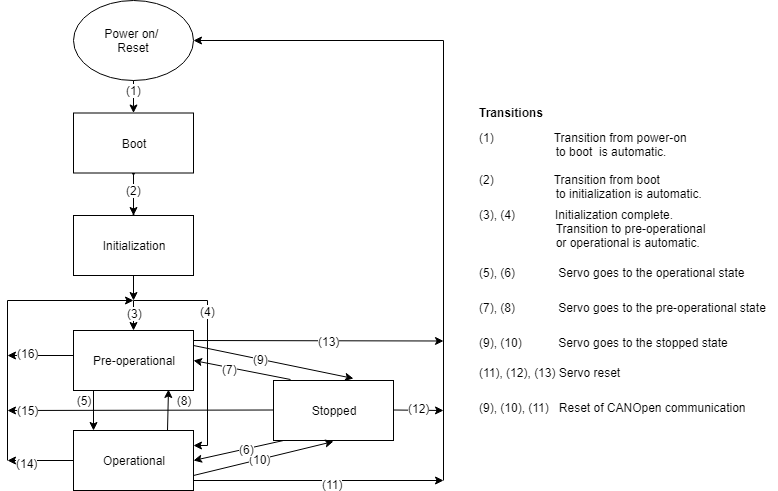
\includegraphics[width=\textwidth,height=\textheight/2,keepaspectratio=true]{nmt_states.png}}
\end{DoxyImageNoCaption}
 \begin{DoxyEnumFields}{Enumerator}
\raisebox{\heightof{T}}[0pt][0pt]{\index{RR\_NMT\_INITIALIZING@{RR\_NMT\_INITIALIZING}!api.h@{api.h}}\index{api.h@{api.h}!RR\_NMT\_INITIALIZING@{RR\_NMT\_INITIALIZING}}}\mbox{\Hypertarget{api_8h_afaf255d20b35be64a488b42e11feab29ac2550cce228ff5512ea417e2b035b665}\label{api_8h_afaf255d20b35be64a488b42e11feab29ac2550cce228ff5512ea417e2b035b665}} 
RR\+\_\+\+NMT\+\_\+\+INITIALIZING&Device is initializing \\
\hline

\raisebox{\heightof{T}}[0pt][0pt]{\index{RR\_NMT\_BOOT@{RR\_NMT\_BOOT}!api.h@{api.h}}\index{api.h@{api.h}!RR\_NMT\_BOOT@{RR\_NMT\_BOOT}}}\mbox{\Hypertarget{api_8h_afaf255d20b35be64a488b42e11feab29a4b2cf9b28688f7985afff0c25a7da61b}\label{api_8h_afaf255d20b35be64a488b42e11feab29a4b2cf9b28688f7985afff0c25a7da61b}} 
RR\+\_\+\+NMT\+\_\+\+BOOT&Device is executing a bootloader application \\
\hline

\raisebox{\heightof{T}}[0pt][0pt]{\index{RR\_NMT\_PRE\_OPERATIONAL@{RR\_NMT\_PRE\_OPERATIONAL}!api.h@{api.h}}\index{api.h@{api.h}!RR\_NMT\_PRE\_OPERATIONAL@{RR\_NMT\_PRE\_OPERATIONAL}}}\mbox{\Hypertarget{api_8h_afaf255d20b35be64a488b42e11feab29ace8deaf0d4ce3230fb48c15de516e474}\label{api_8h_afaf255d20b35be64a488b42e11feab29ace8deaf0d4ce3230fb48c15de516e474}} 
RR\+\_\+\+NMT\+\_\+\+PRE\+\_\+\+OPERATIONAL&Device is in the pre-\/operational state \\
\hline

\raisebox{\heightof{T}}[0pt][0pt]{\index{RR\_NMT\_OPERATIONAL@{RR\_NMT\_OPERATIONAL}!api.h@{api.h}}\index{api.h@{api.h}!RR\_NMT\_OPERATIONAL@{RR\_NMT\_OPERATIONAL}}}\mbox{\Hypertarget{api_8h_afaf255d20b35be64a488b42e11feab29a57e41d0fd4f218c20acc57061b28f52d}\label{api_8h_afaf255d20b35be64a488b42e11feab29a57e41d0fd4f218c20acc57061b28f52d}} 
RR\+\_\+\+NMT\+\_\+\+OPERATIONAL&Device is in the operational state \\
\hline

\raisebox{\heightof{T}}[0pt][0pt]{\index{RR\_NMT\_STOPPED@{RR\_NMT\_STOPPED}!api.h@{api.h}}\index{api.h@{api.h}!RR\_NMT\_STOPPED@{RR\_NMT\_STOPPED}}}\mbox{\Hypertarget{api_8h_afaf255d20b35be64a488b42e11feab29a0b3bd632c9abf67a54795f902b0cb2f8}\label{api_8h_afaf255d20b35be64a488b42e11feab29a0b3bd632c9abf67a54795f902b0cb2f8}} 
RR\+\_\+\+NMT\+\_\+\+STOPPED&Device is in the stopped state \\
\hline

\raisebox{\heightof{T}}[0pt][0pt]{\index{RR\_NMT\_HB\_TIMEOUT@{RR\_NMT\_HB\_TIMEOUT}!api.h@{api.h}}\index{api.h@{api.h}!RR\_NMT\_HB\_TIMEOUT@{RR\_NMT\_HB\_TIMEOUT}}}\mbox{\Hypertarget{api_8h_afaf255d20b35be64a488b42e11feab29af745eff49927034f66cbd67835b2fd26}\label{api_8h_afaf255d20b35be64a488b42e11feab29af745eff49927034f66cbd67835b2fd26}} 
RR\+\_\+\+NMT\+\_\+\+HB\+\_\+\+TIMEOUT&Device Heartbeat timeout (device disappeared from the bus) \\
\hline

\end{DoxyEnumFields}
\mbox{\Hypertarget{api_8h_a92d5be5038abcf89837faf85a08debdc}\label{api_8h_a92d5be5038abcf89837faf85a08debdc}} 
\index{api.h@{api.h}!rr\_ret\_status\_t@{rr\_ret\_status\_t}}
\index{rr\_ret\_status\_t@{rr\_ret\_status\_t}!api.h@{api.h}}
\doxysubsubsection{\texorpdfstring{rr\_ret\_status\_t}{rr\_ret\_status\_t}}
{\footnotesize\ttfamily enum \mbox{\hyperlink{api_8h_a92d5be5038abcf89837faf85a08debdc}{rr\+\_\+ret\+\_\+status\+\_\+t}}}



Return codes of the API functions. 

\begin{DoxyEnumFields}{Enumerator}
\raisebox{\heightof{T}}[0pt][0pt]{\index{RET\_OK@{RET\_OK}!api.h@{api.h}}\index{api.h@{api.h}!RET\_OK@{RET\_OK}}}\mbox{\Hypertarget{api_8h_a92d5be5038abcf89837faf85a08debdca4894234446e2d92068943b3d6d3a0bdc}\label{api_8h_a92d5be5038abcf89837faf85a08debdca4894234446e2d92068943b3d6d3a0bdc}} 
RET\+\_\+\+OK&Status OK. \\
\hline

\raisebox{\heightof{T}}[0pt][0pt]{\index{RET\_ERROR@{RET\_ERROR}!api.h@{api.h}}\index{api.h@{api.h}!RET\_ERROR@{RET\_ERROR}}}\mbox{\Hypertarget{api_8h_a92d5be5038abcf89837faf85a08debdcae8ed27c1aabd77d519426a8ad340d76c}\label{api_8h_a92d5be5038abcf89837faf85a08debdcae8ed27c1aabd77d519426a8ad340d76c}} 
RET\+\_\+\+ERROR&Generic error. \\
\hline

\raisebox{\heightof{T}}[0pt][0pt]{\index{RET\_BAD\_INSTANCE@{RET\_BAD\_INSTANCE}!api.h@{api.h}}\index{api.h@{api.h}!RET\_BAD\_INSTANCE@{RET\_BAD\_INSTANCE}}}\mbox{\Hypertarget{api_8h_a92d5be5038abcf89837faf85a08debdcada2fa397afd6b90ecb1c5b9ca3a2d0ee}\label{api_8h_a92d5be5038abcf89837faf85a08debdcada2fa397afd6b90ecb1c5b9ca3a2d0ee}} 
RET\+\_\+\+BAD\+\_\+\+INSTANCE&Bad interface or servo instance (null) \\
\hline

\raisebox{\heightof{T}}[0pt][0pt]{\index{RET\_BUSY@{RET\_BUSY}!api.h@{api.h}}\index{api.h@{api.h}!RET\_BUSY@{RET\_BUSY}}}\mbox{\Hypertarget{api_8h_a92d5be5038abcf89837faf85a08debdcacdd796ae2972988d689257753a05b9dd}\label{api_8h_a92d5be5038abcf89837faf85a08debdcacdd796ae2972988d689257753a05b9dd}} 
RET\+\_\+\+BUSY&Device is busy. \\
\hline

\raisebox{\heightof{T}}[0pt][0pt]{\index{RET\_WRONG\_TRAJ@{RET\_WRONG\_TRAJ}!api.h@{api.h}}\index{api.h@{api.h}!RET\_WRONG\_TRAJ@{RET\_WRONG\_TRAJ}}}\mbox{\Hypertarget{api_8h_a92d5be5038abcf89837faf85a08debdcadf1d978b055d00c4036019387acfc60c}\label{api_8h_a92d5be5038abcf89837faf85a08debdcadf1d978b055d00c4036019387acfc60c}} 
RET\+\_\+\+WRONG\+\_\+\+TRAJ&Wrong trajectory. \\
\hline

\raisebox{\heightof{T}}[0pt][0pt]{\index{RET\_LOCKED@{RET\_LOCKED}!api.h@{api.h}}\index{api.h@{api.h}!RET\_LOCKED@{RET\_LOCKED}}}\mbox{\Hypertarget{api_8h_a92d5be5038abcf89837faf85a08debdca2840a6ac495b0fe4b9e8565d9f76e29a}\label{api_8h_a92d5be5038abcf89837faf85a08debdca2840a6ac495b0fe4b9e8565d9f76e29a}} 
RET\+\_\+\+LOCKED&Device is locked. \\
\hline

\raisebox{\heightof{T}}[0pt][0pt]{\index{RET\_STOPPED@{RET\_STOPPED}!api.h@{api.h}}\index{api.h@{api.h}!RET\_STOPPED@{RET\_STOPPED}}}\mbox{\Hypertarget{api_8h_a92d5be5038abcf89837faf85a08debdcad456500c4074aeffb3e5e132bf7d996c}\label{api_8h_a92d5be5038abcf89837faf85a08debdcad456500c4074aeffb3e5e132bf7d996c}} 
RET\+\_\+\+STOPPED&Device is in the STOPPED state. \\
\hline

\raisebox{\heightof{T}}[0pt][0pt]{\index{RET\_TIMEOUT@{RET\_TIMEOUT}!api.h@{api.h}}\index{api.h@{api.h}!RET\_TIMEOUT@{RET\_TIMEOUT}}}\mbox{\Hypertarget{api_8h_a92d5be5038abcf89837faf85a08debdcadf2eed18ed159c7517505568b0f261dd}\label{api_8h_a92d5be5038abcf89837faf85a08debdcadf2eed18ed159c7517505568b0f261dd}} 
RET\+\_\+\+TIMEOUT&CAN communication timeout. \\
\hline

\raisebox{\heightof{T}}[0pt][0pt]{\index{RET\_ZERO\_SIZE@{RET\_ZERO\_SIZE}!api.h@{api.h}}\index{api.h@{api.h}!RET\_ZERO\_SIZE@{RET\_ZERO\_SIZE}}}\mbox{\Hypertarget{api_8h_a92d5be5038abcf89837faf85a08debdcac2c7bf0285c804ae03c6628659ce366e}\label{api_8h_a92d5be5038abcf89837faf85a08debdcac2c7bf0285c804ae03c6628659ce366e}} 
RET\+\_\+\+ZERO\+\_\+\+SIZE&Zero data size. \\
\hline

\raisebox{\heightof{T}}[0pt][0pt]{\index{RET\_SIZE\_MISMATCH@{RET\_SIZE\_MISMATCH}!api.h@{api.h}}\index{api.h@{api.h}!RET\_SIZE\_MISMATCH@{RET\_SIZE\_MISMATCH}}}\mbox{\Hypertarget{api_8h_a92d5be5038abcf89837faf85a08debdca639f91af3521a375df0778f9cd60d60b}\label{api_8h_a92d5be5038abcf89837faf85a08debdca639f91af3521a375df0778f9cd60d60b}} 
RET\+\_\+\+SIZE\+\_\+\+MISMATCH&Mismatch of received and target data size. \\
\hline

\raisebox{\heightof{T}}[0pt][0pt]{\index{RET\_WRONG\_ARG@{RET\_WRONG\_ARG}!api.h@{api.h}}\index{api.h@{api.h}!RET\_WRONG\_ARG@{RET\_WRONG\_ARG}}}\mbox{\Hypertarget{api_8h_a92d5be5038abcf89837faf85a08debdca6368c40539ccc8fe56a2b433d13370dc}\label{api_8h_a92d5be5038abcf89837faf85a08debdca6368c40539ccc8fe56a2b433d13370dc}} 
RET\+\_\+\+WRONG\+\_\+\+ARG&Wrong function argument. \\
\hline

\end{DoxyEnumFields}
\mbox{\Hypertarget{api_8h_aa1f58887fab4642cf49f6f453c1d276d}\label{api_8h_aa1f58887fab4642cf49f6f453c1d276d}} 
\index{api.h@{api.h}!rr\_servo\_param\_t@{rr\_servo\_param\_t}}
\index{rr\_servo\_param\_t@{rr\_servo\_param\_t}!api.h@{api.h}}
\doxysubsubsection{\texorpdfstring{rr\_servo\_param\_t}{rr\_servo\_param\_t}}
{\footnotesize\ttfamily enum \mbox{\hyperlink{api_8h_aa1f58887fab4642cf49f6f453c1d276d}{rr\+\_\+servo\+\_\+param\+\_\+t}}}



Device parameter and source indices. 

\begin{DoxyEnumFields}{Enumerator}
\raisebox{\heightof{T}}[0pt][0pt]{\index{APP\_PARAM\_NULL@{APP\_PARAM\_NULL}!api.h@{api.h}}\index{api.h@{api.h}!APP\_PARAM\_NULL@{APP\_PARAM\_NULL}}}\mbox{\Hypertarget{api_8h_aa1f58887fab4642cf49f6f453c1d276daf92693e0b44950ce14a0e4c467ca9d08}\label{api_8h_aa1f58887fab4642cf49f6f453c1d276daf92693e0b44950ce14a0e4c467ca9d08}} 
APP\+\_\+\+PARAM\+\_\+\+NULL&Not used. \\
\hline

\raisebox{\heightof{T}}[0pt][0pt]{\index{APP\_PARAM\_POSITION@{APP\_PARAM\_POSITION}!api.h@{api.h}}\index{api.h@{api.h}!APP\_PARAM\_POSITION@{APP\_PARAM\_POSITION}}}\mbox{\Hypertarget{api_8h_aa1f58887fab4642cf49f6f453c1d276dab079617b03cb882ecb48c06ae6603363}\label{api_8h_aa1f58887fab4642cf49f6f453c1d276dab079617b03cb882ecb48c06ae6603363}} 
APP\+\_\+\+PARAM\+\_\+\+POSITION&Actual multi-\/turn position of the output shaft (degrees) \\
\hline

\raisebox{\heightof{T}}[0pt][0pt]{\index{APP\_PARAM\_VELOCITY@{APP\_PARAM\_VELOCITY}!api.h@{api.h}}\index{api.h@{api.h}!APP\_PARAM\_VELOCITY@{APP\_PARAM\_VELOCITY}}}\mbox{\Hypertarget{api_8h_aa1f58887fab4642cf49f6f453c1d276da7c7eb311e57837875791d5e58982661c}\label{api_8h_aa1f58887fab4642cf49f6f453c1d276da7c7eb311e57837875791d5e58982661c}} 
APP\+\_\+\+PARAM\+\_\+\+VELOCITY&Actual velocity of the output shaft (degrees per second) \\
\hline

\raisebox{\heightof{T}}[0pt][0pt]{\index{APP\_PARAM\_POSITION\_ROTOR@{APP\_PARAM\_POSITION\_ROTOR}!api.h@{api.h}}\index{api.h@{api.h}!APP\_PARAM\_POSITION\_ROTOR@{APP\_PARAM\_POSITION\_ROTOR}}}\mbox{\Hypertarget{api_8h_aa1f58887fab4642cf49f6f453c1d276daa8dafaaa373617ef2f8585b3d4177115}\label{api_8h_aa1f58887fab4642cf49f6f453c1d276daa8dafaaa373617ef2f8585b3d4177115}} 
APP\+\_\+\+PARAM\+\_\+\+POSITION\+\_\+\+ROTOR&Actual position of the motor shaft (degrees) \\
\hline

\raisebox{\heightof{T}}[0pt][0pt]{\index{APP\_PARAM\_VELOCITY\_ROTOR@{APP\_PARAM\_VELOCITY\_ROTOR}!api.h@{api.h}}\index{api.h@{api.h}!APP\_PARAM\_VELOCITY\_ROTOR@{APP\_PARAM\_VELOCITY\_ROTOR}}}\mbox{\Hypertarget{api_8h_aa1f58887fab4642cf49f6f453c1d276dade3db1d484cf6dd69b115e37ab77051b}\label{api_8h_aa1f58887fab4642cf49f6f453c1d276dade3db1d484cf6dd69b115e37ab77051b}} 
APP\+\_\+\+PARAM\+\_\+\+VELOCITY\+\_\+\+ROTOR&Actual velocity of the motor shaft (degrees per second) \\
\hline

\raisebox{\heightof{T}}[0pt][0pt]{\index{APP\_PARAM\_POSITION\_GEAR\_360@{APP\_PARAM\_POSITION\_GEAR\_360}!api.h@{api.h}}\index{api.h@{api.h}!APP\_PARAM\_POSITION\_GEAR\_360@{APP\_PARAM\_POSITION\_GEAR\_360}}}\mbox{\Hypertarget{api_8h_aa1f58887fab4642cf49f6f453c1d276dab8e557b8564d2bf579cc199b343644f2}\label{api_8h_aa1f58887fab4642cf49f6f453c1d276dab8e557b8564d2bf579cc199b343644f2}} 
APP\+\_\+\+PARAM\+\_\+\+POSITION\+\_\+\+GEAR\+\_\+360&Actual single-\/turn position of the output shaft (from 0 to 360 degrees) \\
\hline

\raisebox{\heightof{T}}[0pt][0pt]{\index{APP\_PARAM\_POSITION\_GEAR\_EMULATED@{APP\_PARAM\_POSITION\_GEAR\_EMULATED}!api.h@{api.h}}\index{api.h@{api.h}!APP\_PARAM\_POSITION\_GEAR\_EMULATED@{APP\_PARAM\_POSITION\_GEAR\_EMULATED}}}\mbox{\Hypertarget{api_8h_aa1f58887fab4642cf49f6f453c1d276da27cb6c1302d1ed7545ee8c8ee020b9c1}\label{api_8h_aa1f58887fab4642cf49f6f453c1d276da27cb6c1302d1ed7545ee8c8ee020b9c1}} 
APP\+\_\+\+PARAM\+\_\+\+POSITION\+\_\+\+GEAR\+\_\+\+EMULATED&Actual multi-\/turn position of the motor shaft multiplied by gear ratio (degrees) \\
\hline

\raisebox{\heightof{T}}[0pt][0pt]{\index{APP\_PARAM\_CURRENT\_INPUT@{APP\_PARAM\_CURRENT\_INPUT}!api.h@{api.h}}\index{api.h@{api.h}!APP\_PARAM\_CURRENT\_INPUT@{APP\_PARAM\_CURRENT\_INPUT}}}\mbox{\Hypertarget{api_8h_aa1f58887fab4642cf49f6f453c1d276dafb1be8c565208f94596b980788ac52fe}\label{api_8h_aa1f58887fab4642cf49f6f453c1d276dafb1be8c565208f94596b980788ac52fe}} 
APP\+\_\+\+PARAM\+\_\+\+CURRENT\+\_\+\+INPUT&Actual DC current (Amperes) in the servo\textquotesingle{}s supply circuit. \\
\hline

\raisebox{\heightof{T}}[0pt][0pt]{\index{APP\_PARAM\_CURRENT\_OUTPUT@{APP\_PARAM\_CURRENT\_OUTPUT}!api.h@{api.h}}\index{api.h@{api.h}!APP\_PARAM\_CURRENT\_OUTPUT@{APP\_PARAM\_CURRENT\_OUTPUT}}}\mbox{\Hypertarget{api_8h_aa1f58887fab4642cf49f6f453c1d276dae8c5d203df5baa3a329b89e4e3c05e31}\label{api_8h_aa1f58887fab4642cf49f6f453c1d276dae8c5d203df5baa3a329b89e4e3c05e31}} 
APP\+\_\+\+PARAM\+\_\+\+CURRENT\+\_\+\+OUTPUT&Not used. \\
\hline

\raisebox{\heightof{T}}[0pt][0pt]{\index{APP\_PARAM\_VOLTAGE\_INPUT@{APP\_PARAM\_VOLTAGE\_INPUT}!api.h@{api.h}}\index{api.h@{api.h}!APP\_PARAM\_VOLTAGE\_INPUT@{APP\_PARAM\_VOLTAGE\_INPUT}}}\mbox{\Hypertarget{api_8h_aa1f58887fab4642cf49f6f453c1d276da78bc54701f1fe1ce6b90b70bbfa62483}\label{api_8h_aa1f58887fab4642cf49f6f453c1d276da78bc54701f1fe1ce6b90b70bbfa62483}} 
APP\+\_\+\+PARAM\+\_\+\+VOLTAGE\+\_\+\+INPUT&Actual DC voltage (Volts) supplied to the servo. \\
\hline

\raisebox{\heightof{T}}[0pt][0pt]{\index{APP\_PARAM\_VOLTAGE\_OUTPUT@{APP\_PARAM\_VOLTAGE\_OUTPUT}!api.h@{api.h}}\index{api.h@{api.h}!APP\_PARAM\_VOLTAGE\_OUTPUT@{APP\_PARAM\_VOLTAGE\_OUTPUT}}}\mbox{\Hypertarget{api_8h_aa1f58887fab4642cf49f6f453c1d276da09d81b3e2fccfa745188ab46c8dd7263}\label{api_8h_aa1f58887fab4642cf49f6f453c1d276da09d81b3e2fccfa745188ab46c8dd7263}} 
APP\+\_\+\+PARAM\+\_\+\+VOLTAGE\+\_\+\+OUTPUT&Not used. \\
\hline

\raisebox{\heightof{T}}[0pt][0pt]{\index{APP\_PARAM\_CURRENT\_PHASE@{APP\_PARAM\_CURRENT\_PHASE}!api.h@{api.h}}\index{api.h@{api.h}!APP\_PARAM\_CURRENT\_PHASE@{APP\_PARAM\_CURRENT\_PHASE}}}\mbox{\Hypertarget{api_8h_aa1f58887fab4642cf49f6f453c1d276dad60719b243d4c9abd6c6c2566266fa52}\label{api_8h_aa1f58887fab4642cf49f6f453c1d276dad60719b243d4c9abd6c6c2566266fa52}} 
APP\+\_\+\+PARAM\+\_\+\+CURRENT\+\_\+\+PHASE&Actual magnitude of AC current (Amperes) on the motor. \\
\hline

\raisebox{\heightof{T}}[0pt][0pt]{\index{APP\_PARAM\_TEMPERATURE\_ACTUATOR@{APP\_PARAM\_TEMPERATURE\_ACTUATOR}!api.h@{api.h}}\index{api.h@{api.h}!APP\_PARAM\_TEMPERATURE\_ACTUATOR@{APP\_PARAM\_TEMPERATURE\_ACTUATOR}}}\mbox{\Hypertarget{api_8h_aa1f58887fab4642cf49f6f453c1d276da1a3c86ed7fe187d364809094d3c1dc3a}\label{api_8h_aa1f58887fab4642cf49f6f453c1d276da1a3c86ed7fe187d364809094d3c1dc3a}} 
APP\+\_\+\+PARAM\+\_\+\+TEMPERATURE\+\_\+\+ACTUATOR&Not used. \\
\hline

\raisebox{\heightof{T}}[0pt][0pt]{\index{APP\_PARAM\_TEMPERATURE\_ELECTRONICS@{APP\_PARAM\_TEMPERATURE\_ELECTRONICS}!api.h@{api.h}}\index{api.h@{api.h}!APP\_PARAM\_TEMPERATURE\_ELECTRONICS@{APP\_PARAM\_TEMPERATURE\_ELECTRONICS}}}\mbox{\Hypertarget{api_8h_aa1f58887fab4642cf49f6f453c1d276da48d8972dac6ee7ea647431a83dd88143}\label{api_8h_aa1f58887fab4642cf49f6f453c1d276da48d8972dac6ee7ea647431a83dd88143}} 
APP\+\_\+\+PARAM\+\_\+\+TEMPERATURE\+\_\+\+ELECTRONICS&Actual temperature of the motor controller. \\
\hline

\raisebox{\heightof{T}}[0pt][0pt]{\index{APP\_PARAM\_TORQUE@{APP\_PARAM\_TORQUE}!api.h@{api.h}}\index{api.h@{api.h}!APP\_PARAM\_TORQUE@{APP\_PARAM\_TORQUE}}}\mbox{\Hypertarget{api_8h_aa1f58887fab4642cf49f6f453c1d276da5bc9d6003879b42f41d8db8ee443afbf}\label{api_8h_aa1f58887fab4642cf49f6f453c1d276da5bc9d6003879b42f41d8db8ee443afbf}} 
APP\+\_\+\+PARAM\+\_\+\+TORQUE&Not used. \\
\hline

\raisebox{\heightof{T}}[0pt][0pt]{\index{APP\_PARAM\_ACCELERATION@{APP\_PARAM\_ACCELERATION}!api.h@{api.h}}\index{api.h@{api.h}!APP\_PARAM\_ACCELERATION@{APP\_PARAM\_ACCELERATION}}}\mbox{\Hypertarget{api_8h_aa1f58887fab4642cf49f6f453c1d276dae433fe695af5d074e34503e78802e79c}\label{api_8h_aa1f58887fab4642cf49f6f453c1d276dae433fe695af5d074e34503e78802e79c}} 
APP\+\_\+\+PARAM\+\_\+\+ACCELERATION&Not used. \\
\hline

\raisebox{\heightof{T}}[0pt][0pt]{\index{APP\_PARAM\_ACCELERATION\_ROTOR@{APP\_PARAM\_ACCELERATION\_ROTOR}!api.h@{api.h}}\index{api.h@{api.h}!APP\_PARAM\_ACCELERATION\_ROTOR@{APP\_PARAM\_ACCELERATION\_ROTOR}}}\mbox{\Hypertarget{api_8h_aa1f58887fab4642cf49f6f453c1d276da6f9d3e5a018689702d2f070888af6882}\label{api_8h_aa1f58887fab4642cf49f6f453c1d276da6f9d3e5a018689702d2f070888af6882}} 
APP\+\_\+\+PARAM\+\_\+\+ACCELERATION\+\_\+\+ROTOR&Not used. \\
\hline

\raisebox{\heightof{T}}[0pt][0pt]{\index{APP\_PARAM\_CURRENT\_PHASE\_1@{APP\_PARAM\_CURRENT\_PHASE\_1}!api.h@{api.h}}\index{api.h@{api.h}!APP\_PARAM\_CURRENT\_PHASE\_1@{APP\_PARAM\_CURRENT\_PHASE\_1}}}\mbox{\Hypertarget{api_8h_aa1f58887fab4642cf49f6f453c1d276dae2db7f59e354f0adf411ebc097be9615}\label{api_8h_aa1f58887fab4642cf49f6f453c1d276dae2db7f59e354f0adf411ebc097be9615}} 
APP\+\_\+\+PARAM\+\_\+\+CURRENT\+\_\+\+PHASE\+\_\+1&Actual phase 1 current to the motor. \\
\hline

\raisebox{\heightof{T}}[0pt][0pt]{\index{APP\_PARAM\_CURRENT\_PHASE\_2@{APP\_PARAM\_CURRENT\_PHASE\_2}!api.h@{api.h}}\index{api.h@{api.h}!APP\_PARAM\_CURRENT\_PHASE\_2@{APP\_PARAM\_CURRENT\_PHASE\_2}}}\mbox{\Hypertarget{api_8h_aa1f58887fab4642cf49f6f453c1d276daecd1a50b950e607328843d7ab44ef37b}\label{api_8h_aa1f58887fab4642cf49f6f453c1d276daecd1a50b950e607328843d7ab44ef37b}} 
APP\+\_\+\+PARAM\+\_\+\+CURRENT\+\_\+\+PHASE\+\_\+2&Actual phase 2 current to the motor. \\
\hline

\raisebox{\heightof{T}}[0pt][0pt]{\index{APP\_PARAM\_CURRENT\_PHASE\_3@{APP\_PARAM\_CURRENT\_PHASE\_3}!api.h@{api.h}}\index{api.h@{api.h}!APP\_PARAM\_CURRENT\_PHASE\_3@{APP\_PARAM\_CURRENT\_PHASE\_3}}}\mbox{\Hypertarget{api_8h_aa1f58887fab4642cf49f6f453c1d276daf52784c6a104216ecddc02d08edca79b}\label{api_8h_aa1f58887fab4642cf49f6f453c1d276daf52784c6a104216ecddc02d08edca79b}} 
APP\+\_\+\+PARAM\+\_\+\+CURRENT\+\_\+\+PHASE\+\_\+3&Actual phase 3 current to the motor. \\
\hline

\raisebox{\heightof{T}}[0pt][0pt]{\index{APP\_PARAM\_CURRENT\_RAW@{APP\_PARAM\_CURRENT\_RAW}!api.h@{api.h}}\index{api.h@{api.h}!APP\_PARAM\_CURRENT\_RAW@{APP\_PARAM\_CURRENT\_RAW}}}\mbox{\Hypertarget{api_8h_aa1f58887fab4642cf49f6f453c1d276da2612f6ba14c9dd0ad30ac7d67c3a9707}\label{api_8h_aa1f58887fab4642cf49f6f453c1d276da2612f6ba14c9dd0ad30ac7d67c3a9707}} 
APP\+\_\+\+PARAM\+\_\+\+CURRENT\+\_\+\+RAW&Not used. \\
\hline

\raisebox{\heightof{T}}[0pt][0pt]{\index{APP\_PARAM\_CURRENT\_RAW\_2@{APP\_PARAM\_CURRENT\_RAW\_2}!api.h@{api.h}}\index{api.h@{api.h}!APP\_PARAM\_CURRENT\_RAW\_2@{APP\_PARAM\_CURRENT\_RAW\_2}}}\mbox{\Hypertarget{api_8h_aa1f58887fab4642cf49f6f453c1d276daa28d107cc1bfbff653eee6bc0abc9df1}\label{api_8h_aa1f58887fab4642cf49f6f453c1d276daa28d107cc1bfbff653eee6bc0abc9df1}} 
APP\+\_\+\+PARAM\+\_\+\+CURRENT\+\_\+\+RAW\+\_\+2&Not used. \\
\hline

\raisebox{\heightof{T}}[0pt][0pt]{\index{APP\_PARAM\_CURRENT\_RAW\_3@{APP\_PARAM\_CURRENT\_RAW\_3}!api.h@{api.h}}\index{api.h@{api.h}!APP\_PARAM\_CURRENT\_RAW\_3@{APP\_PARAM\_CURRENT\_RAW\_3}}}\mbox{\Hypertarget{api_8h_aa1f58887fab4642cf49f6f453c1d276da44c5166f84bc671786688186ca4f34d0}\label{api_8h_aa1f58887fab4642cf49f6f453c1d276da44c5166f84bc671786688186ca4f34d0}} 
APP\+\_\+\+PARAM\+\_\+\+CURRENT\+\_\+\+RAW\+\_\+3&Not used. \\
\hline

\raisebox{\heightof{T}}[0pt][0pt]{\index{APP\_PARAM\_ENCODER\_MASTER\_TRACK@{APP\_PARAM\_ENCODER\_MASTER\_TRACK}!api.h@{api.h}}\index{api.h@{api.h}!APP\_PARAM\_ENCODER\_MASTER\_TRACK@{APP\_PARAM\_ENCODER\_MASTER\_TRACK}}}\mbox{\Hypertarget{api_8h_aa1f58887fab4642cf49f6f453c1d276da882f43f6b3595fe0a321f208a41d726e}\label{api_8h_aa1f58887fab4642cf49f6f453c1d276da882f43f6b3595fe0a321f208a41d726e}} 
APP\+\_\+\+PARAM\+\_\+\+ENCODER\+\_\+\+MASTER\+\_\+\+TRACK&Internal use only. \\
\hline

\raisebox{\heightof{T}}[0pt][0pt]{\index{APP\_PARAM\_ENCODER\_NONIUS\_TRACK@{APP\_PARAM\_ENCODER\_NONIUS\_TRACK}!api.h@{api.h}}\index{api.h@{api.h}!APP\_PARAM\_ENCODER\_NONIUS\_TRACK@{APP\_PARAM\_ENCODER\_NONIUS\_TRACK}}}\mbox{\Hypertarget{api_8h_aa1f58887fab4642cf49f6f453c1d276da3facac23b091243602b47fd2576b2823}\label{api_8h_aa1f58887fab4642cf49f6f453c1d276da3facac23b091243602b47fd2576b2823}} 
APP\+\_\+\+PARAM\+\_\+\+ENCODER\+\_\+\+NONIUS\+\_\+\+TRACK&Internal use only. \\
\hline

\raisebox{\heightof{T}}[0pt][0pt]{\index{APP\_PARAM\_ENCODER\_MOTOR\_MASTER\_TRACK@{APP\_PARAM\_ENCODER\_MOTOR\_MASTER\_TRACK}!api.h@{api.h}}\index{api.h@{api.h}!APP\_PARAM\_ENCODER\_MOTOR\_MASTER\_TRACK@{APP\_PARAM\_ENCODER\_MOTOR\_MASTER\_TRACK}}}\mbox{\Hypertarget{api_8h_aa1f58887fab4642cf49f6f453c1d276da9abecc57566475fa5d0a47a30d3eb7b7}\label{api_8h_aa1f58887fab4642cf49f6f453c1d276da9abecc57566475fa5d0a47a30d3eb7b7}} 
APP\+\_\+\+PARAM\+\_\+\+ENCODER\+\_\+\+MOTOR\+\_\+\+MASTER\+\_\+\+TRACK&Internal use only. \\
\hline

\raisebox{\heightof{T}}[0pt][0pt]{\index{APP\_PARAM\_ENCODER\_MOTOR\_NONIUS\_TRACK@{APP\_PARAM\_ENCODER\_MOTOR\_NONIUS\_TRACK}!api.h@{api.h}}\index{api.h@{api.h}!APP\_PARAM\_ENCODER\_MOTOR\_NONIUS\_TRACK@{APP\_PARAM\_ENCODER\_MOTOR\_NONIUS\_TRACK}}}\mbox{\Hypertarget{api_8h_aa1f58887fab4642cf49f6f453c1d276dad2803d24470187ed238ad95997bfe9be}\label{api_8h_aa1f58887fab4642cf49f6f453c1d276dad2803d24470187ed238ad95997bfe9be}} 
APP\+\_\+\+PARAM\+\_\+\+ENCODER\+\_\+\+MOTOR\+\_\+\+NONIUS\+\_\+\+TRACK&Internal use only. \\
\hline

\raisebox{\heightof{T}}[0pt][0pt]{\index{APP\_PARAM\_TORQUE\_ELECTRIC\_CALC@{APP\_PARAM\_TORQUE\_ELECTRIC\_CALC}!api.h@{api.h}}\index{api.h@{api.h}!APP\_PARAM\_TORQUE\_ELECTRIC\_CALC@{APP\_PARAM\_TORQUE\_ELECTRIC\_CALC}}}\mbox{\Hypertarget{api_8h_aa1f58887fab4642cf49f6f453c1d276da354f3004c944556f129c2b590b80c629}\label{api_8h_aa1f58887fab4642cf49f6f453c1d276da354f3004c944556f129c2b590b80c629}} 
APP\+\_\+\+PARAM\+\_\+\+TORQUE\+\_\+\+ELECTRIC\+\_\+\+CALC&Internal use only. \\
\hline

\raisebox{\heightof{T}}[0pt][0pt]{\index{APP\_PARAM\_CONTROLLER\_VELOCITY\_ERROR@{APP\_PARAM\_CONTROLLER\_VELOCITY\_ERROR}!api.h@{api.h}}\index{api.h@{api.h}!APP\_PARAM\_CONTROLLER\_VELOCITY\_ERROR@{APP\_PARAM\_CONTROLLER\_VELOCITY\_ERROR}}}\mbox{\Hypertarget{api_8h_aa1f58887fab4642cf49f6f453c1d276dae48e6cfbaff81ae1166e684b004f868d}\label{api_8h_aa1f58887fab4642cf49f6f453c1d276dae48e6cfbaff81ae1166e684b004f868d}} 
APP\+\_\+\+PARAM\+\_\+\+CONTROLLER\+\_\+\+VELOCITY\+\_\+\+ERROR&Velocity following error (difference in degrees per second between the setpoint and feedback velocities) \\
\hline

\raisebox{\heightof{T}}[0pt][0pt]{\index{APP\_PARAM\_CONTROLLER\_VELOCITY\_SETPOINT@{APP\_PARAM\_CONTROLLER\_VELOCITY\_SETPOINT}!api.h@{api.h}}\index{api.h@{api.h}!APP\_PARAM\_CONTROLLER\_VELOCITY\_SETPOINT@{APP\_PARAM\_CONTROLLER\_VELOCITY\_SETPOINT}}}\mbox{\Hypertarget{api_8h_aa1f58887fab4642cf49f6f453c1d276da91fd08d4408a3251703cef5153b6006e}\label{api_8h_aa1f58887fab4642cf49f6f453c1d276da91fd08d4408a3251703cef5153b6006e}} 
APP\+\_\+\+PARAM\+\_\+\+CONTROLLER\+\_\+\+VELOCITY\+\_\+\+SETPOINT&Velocity target (degrees per second) \\
\hline

\raisebox{\heightof{T}}[0pt][0pt]{\index{APP\_PARAM\_CONTROLLER\_VELOCITY\_FEEDBACK@{APP\_PARAM\_CONTROLLER\_VELOCITY\_FEEDBACK}!api.h@{api.h}}\index{api.h@{api.h}!APP\_PARAM\_CONTROLLER\_VELOCITY\_FEEDBACK@{APP\_PARAM\_CONTROLLER\_VELOCITY\_FEEDBACK}}}\mbox{\Hypertarget{api_8h_aa1f58887fab4642cf49f6f453c1d276da0434a3f113392ee4eefc32a78c61b52b}\label{api_8h_aa1f58887fab4642cf49f6f453c1d276da0434a3f113392ee4eefc32a78c61b52b}} 
APP\+\_\+\+PARAM\+\_\+\+CONTROLLER\+\_\+\+VELOCITY\+\_\+\+FEEDBACK&Actual velocity (degrees per second) \\
\hline

\raisebox{\heightof{T}}[0pt][0pt]{\index{APP\_PARAM\_CONTROLLER\_VELOCITY\_OUTPUT@{APP\_PARAM\_CONTROLLER\_VELOCITY\_OUTPUT}!api.h@{api.h}}\index{api.h@{api.h}!APP\_PARAM\_CONTROLLER\_VELOCITY\_OUTPUT@{APP\_PARAM\_CONTROLLER\_VELOCITY\_OUTPUT}}}\mbox{\Hypertarget{api_8h_aa1f58887fab4642cf49f6f453c1d276da8b6cbe796f36ba0e86a09a21c04c65f5}\label{api_8h_aa1f58887fab4642cf49f6f453c1d276da8b6cbe796f36ba0e86a09a21c04c65f5}} 
APP\+\_\+\+PARAM\+\_\+\+CONTROLLER\+\_\+\+VELOCITY\+\_\+\+OUTPUT&Not used. \\
\hline

\raisebox{\heightof{T}}[0pt][0pt]{\index{APP\_PARAM\_CONTROLLER\_POSITION\_ERROR@{APP\_PARAM\_CONTROLLER\_POSITION\_ERROR}!api.h@{api.h}}\index{api.h@{api.h}!APP\_PARAM\_CONTROLLER\_POSITION\_ERROR@{APP\_PARAM\_CONTROLLER\_POSITION\_ERROR}}}\mbox{\Hypertarget{api_8h_aa1f58887fab4642cf49f6f453c1d276da56a3f7c3f40262a8e771a19ecda28336}\label{api_8h_aa1f58887fab4642cf49f6f453c1d276da56a3f7c3f40262a8e771a19ecda28336}} 
APP\+\_\+\+PARAM\+\_\+\+CONTROLLER\+\_\+\+POSITION\+\_\+\+ERROR&Position following error (difference in degrees per second between the setpoint and feedback velocities) \\
\hline

\raisebox{\heightof{T}}[0pt][0pt]{\index{APP\_PARAM\_CONTROLLER\_POSITION\_SETPOINT@{APP\_PARAM\_CONTROLLER\_POSITION\_SETPOINT}!api.h@{api.h}}\index{api.h@{api.h}!APP\_PARAM\_CONTROLLER\_POSITION\_SETPOINT@{APP\_PARAM\_CONTROLLER\_POSITION\_SETPOINT}}}\mbox{\Hypertarget{api_8h_aa1f58887fab4642cf49f6f453c1d276da25c849d6776790828eec0884f4e1a4ec}\label{api_8h_aa1f58887fab4642cf49f6f453c1d276da25c849d6776790828eec0884f4e1a4ec}} 
APP\+\_\+\+PARAM\+\_\+\+CONTROLLER\+\_\+\+POSITION\+\_\+\+SETPOINT&Position target (degrees) \\
\hline

\raisebox{\heightof{T}}[0pt][0pt]{\index{APP\_PARAM\_CONTROLLER\_POSITION\_FEEDBACK@{APP\_PARAM\_CONTROLLER\_POSITION\_FEEDBACK}!api.h@{api.h}}\index{api.h@{api.h}!APP\_PARAM\_CONTROLLER\_POSITION\_FEEDBACK@{APP\_PARAM\_CONTROLLER\_POSITION\_FEEDBACK}}}\mbox{\Hypertarget{api_8h_aa1f58887fab4642cf49f6f453c1d276da3020332205840419d9e853fc91a77150}\label{api_8h_aa1f58887fab4642cf49f6f453c1d276da3020332205840419d9e853fc91a77150}} 
APP\+\_\+\+PARAM\+\_\+\+CONTROLLER\+\_\+\+POSITION\+\_\+\+FEEDBACK&Actual position (degrees) \\
\hline

\raisebox{\heightof{T}}[0pt][0pt]{\index{APP\_PARAM\_CONTROLLER\_POSITION\_OUTPUT@{APP\_PARAM\_CONTROLLER\_POSITION\_OUTPUT}!api.h@{api.h}}\index{api.h@{api.h}!APP\_PARAM\_CONTROLLER\_POSITION\_OUTPUT@{APP\_PARAM\_CONTROLLER\_POSITION\_OUTPUT}}}\mbox{\Hypertarget{api_8h_aa1f58887fab4642cf49f6f453c1d276da499b7b92c7d38ca32bfad3f774b69bf2}\label{api_8h_aa1f58887fab4642cf49f6f453c1d276da499b7b92c7d38ca32bfad3f774b69bf2}} 
APP\+\_\+\+PARAM\+\_\+\+CONTROLLER\+\_\+\+POSITION\+\_\+\+OUTPUT&Not used. \\
\hline

\raisebox{\heightof{T}}[0pt][0pt]{\index{APP\_PARAM\_CONTROL\_MODE@{APP\_PARAM\_CONTROL\_MODE}!api.h@{api.h}}\index{api.h@{api.h}!APP\_PARAM\_CONTROL\_MODE@{APP\_PARAM\_CONTROL\_MODE}}}\mbox{\Hypertarget{api_8h_aa1f58887fab4642cf49f6f453c1d276da486101d3961797df2f71d944e09806fc}\label{api_8h_aa1f58887fab4642cf49f6f453c1d276da486101d3961797df2f71d944e09806fc}} 
APP\+\_\+\+PARAM\+\_\+\+CONTROL\+\_\+\+MODE&Internal use only. \\
\hline

\raisebox{\heightof{T}}[0pt][0pt]{\index{APP\_PARAM\_FOC\_ANGLE@{APP\_PARAM\_FOC\_ANGLE}!api.h@{api.h}}\index{api.h@{api.h}!APP\_PARAM\_FOC\_ANGLE@{APP\_PARAM\_FOC\_ANGLE}}}\mbox{\Hypertarget{api_8h_aa1f58887fab4642cf49f6f453c1d276da5d39d5f2d4ec671512f0fb2c3d909cb7}\label{api_8h_aa1f58887fab4642cf49f6f453c1d276da5d39d5f2d4ec671512f0fb2c3d909cb7}} 
APP\+\_\+\+PARAM\+\_\+\+FOC\+\_\+\+ANGLE&Internal use only. \\
\hline

\raisebox{\heightof{T}}[0pt][0pt]{\index{APP\_PARAM\_FOC\_IA@{APP\_PARAM\_FOC\_IA}!api.h@{api.h}}\index{api.h@{api.h}!APP\_PARAM\_FOC\_IA@{APP\_PARAM\_FOC\_IA}}}\mbox{\Hypertarget{api_8h_aa1f58887fab4642cf49f6f453c1d276dadb088007a4cbbb03059abe3fe7146dd1}\label{api_8h_aa1f58887fab4642cf49f6f453c1d276dadb088007a4cbbb03059abe3fe7146dd1}} 
APP\+\_\+\+PARAM\+\_\+\+FOC\+\_\+\+IA&Internal use only. \\
\hline

\raisebox{\heightof{T}}[0pt][0pt]{\index{APP\_PARAM\_FOC\_IB@{APP\_PARAM\_FOC\_IB}!api.h@{api.h}}\index{api.h@{api.h}!APP\_PARAM\_FOC\_IB@{APP\_PARAM\_FOC\_IB}}}\mbox{\Hypertarget{api_8h_aa1f58887fab4642cf49f6f453c1d276dad467e8050746e3ee7c4ec2feacc3bd3c}\label{api_8h_aa1f58887fab4642cf49f6f453c1d276dad467e8050746e3ee7c4ec2feacc3bd3c}} 
APP\+\_\+\+PARAM\+\_\+\+FOC\+\_\+\+IB&Internal use only. \\
\hline

\raisebox{\heightof{T}}[0pt][0pt]{\index{APP\_PARAM\_FOC\_IQ\_SET@{APP\_PARAM\_FOC\_IQ\_SET}!api.h@{api.h}}\index{api.h@{api.h}!APP\_PARAM\_FOC\_IQ\_SET@{APP\_PARAM\_FOC\_IQ\_SET}}}\mbox{\Hypertarget{api_8h_aa1f58887fab4642cf49f6f453c1d276da01758ca2594861bbda0763f325ca3aca}\label{api_8h_aa1f58887fab4642cf49f6f453c1d276da01758ca2594861bbda0763f325ca3aca}} 
APP\+\_\+\+PARAM\+\_\+\+FOC\+\_\+\+IQ\+\_\+\+SET&Internal use only. \\
\hline

\raisebox{\heightof{T}}[0pt][0pt]{\index{APP\_PARAM\_FOC\_ID\_SET@{APP\_PARAM\_FOC\_ID\_SET}!api.h@{api.h}}\index{api.h@{api.h}!APP\_PARAM\_FOC\_ID\_SET@{APP\_PARAM\_FOC\_ID\_SET}}}\mbox{\Hypertarget{api_8h_aa1f58887fab4642cf49f6f453c1d276da6f42d9552fbac9730024cca43523a242}\label{api_8h_aa1f58887fab4642cf49f6f453c1d276da6f42d9552fbac9730024cca43523a242}} 
APP\+\_\+\+PARAM\+\_\+\+FOC\+\_\+\+ID\+\_\+\+SET&Internal use only. \\
\hline

\raisebox{\heightof{T}}[0pt][0pt]{\index{APP\_PARAM\_FOC\_IQ@{APP\_PARAM\_FOC\_IQ}!api.h@{api.h}}\index{api.h@{api.h}!APP\_PARAM\_FOC\_IQ@{APP\_PARAM\_FOC\_IQ}}}\mbox{\Hypertarget{api_8h_aa1f58887fab4642cf49f6f453c1d276da73f70b69632299140d13b5c478adc7b4}\label{api_8h_aa1f58887fab4642cf49f6f453c1d276da73f70b69632299140d13b5c478adc7b4}} 
APP\+\_\+\+PARAM\+\_\+\+FOC\+\_\+\+IQ&Internal use only. \\
\hline

\raisebox{\heightof{T}}[0pt][0pt]{\index{APP\_PARAM\_FOC\_ID@{APP\_PARAM\_FOC\_ID}!api.h@{api.h}}\index{api.h@{api.h}!APP\_PARAM\_FOC\_ID@{APP\_PARAM\_FOC\_ID}}}\mbox{\Hypertarget{api_8h_aa1f58887fab4642cf49f6f453c1d276da319baaf4a82176f75f0a8f8cc087a5d7}\label{api_8h_aa1f58887fab4642cf49f6f453c1d276da319baaf4a82176f75f0a8f8cc087a5d7}} 
APP\+\_\+\+PARAM\+\_\+\+FOC\+\_\+\+ID&Internal use only. \\
\hline

\raisebox{\heightof{T}}[0pt][0pt]{\index{APP\_PARAM\_FOC\_IQ\_ERROR@{APP\_PARAM\_FOC\_IQ\_ERROR}!api.h@{api.h}}\index{api.h@{api.h}!APP\_PARAM\_FOC\_IQ\_ERROR@{APP\_PARAM\_FOC\_IQ\_ERROR}}}\mbox{\Hypertarget{api_8h_aa1f58887fab4642cf49f6f453c1d276dacdba14f6f1bc732d0ccae9bc815e0bd2}\label{api_8h_aa1f58887fab4642cf49f6f453c1d276dacdba14f6f1bc732d0ccae9bc815e0bd2}} 
APP\+\_\+\+PARAM\+\_\+\+FOC\+\_\+\+IQ\+\_\+\+ERROR&Internal use only. \\
\hline

\raisebox{\heightof{T}}[0pt][0pt]{\index{APP\_PARAM\_FOC\_ID\_ERROR@{APP\_PARAM\_FOC\_ID\_ERROR}!api.h@{api.h}}\index{api.h@{api.h}!APP\_PARAM\_FOC\_ID\_ERROR@{APP\_PARAM\_FOC\_ID\_ERROR}}}\mbox{\Hypertarget{api_8h_aa1f58887fab4642cf49f6f453c1d276da86ce5142afb8969bc5bc47e4c081d5e3}\label{api_8h_aa1f58887fab4642cf49f6f453c1d276da86ce5142afb8969bc5bc47e4c081d5e3}} 
APP\+\_\+\+PARAM\+\_\+\+FOC\+\_\+\+ID\+\_\+\+ERROR&Internal use only. \\
\hline

\raisebox{\heightof{T}}[0pt][0pt]{\index{APP\_PARAM\_FOC\_UQ@{APP\_PARAM\_FOC\_UQ}!api.h@{api.h}}\index{api.h@{api.h}!APP\_PARAM\_FOC\_UQ@{APP\_PARAM\_FOC\_UQ}}}\mbox{\Hypertarget{api_8h_aa1f58887fab4642cf49f6f453c1d276da9fbb32722da1e00d15978c4c7d2e79c2}\label{api_8h_aa1f58887fab4642cf49f6f453c1d276da9fbb32722da1e00d15978c4c7d2e79c2}} 
APP\+\_\+\+PARAM\+\_\+\+FOC\+\_\+\+UQ&Internal use only. \\
\hline

\raisebox{\heightof{T}}[0pt][0pt]{\index{APP\_PARAM\_FOC\_UD@{APP\_PARAM\_FOC\_UD}!api.h@{api.h}}\index{api.h@{api.h}!APP\_PARAM\_FOC\_UD@{APP\_PARAM\_FOC\_UD}}}\mbox{\Hypertarget{api_8h_aa1f58887fab4642cf49f6f453c1d276da6061e4dd81c828196553b88062a62ada}\label{api_8h_aa1f58887fab4642cf49f6f453c1d276da6061e4dd81c828196553b88062a62ada}} 
APP\+\_\+\+PARAM\+\_\+\+FOC\+\_\+\+UD&Internal use only. \\
\hline

\raisebox{\heightof{T}}[0pt][0pt]{\index{APP\_PARAM\_FOC\_UA@{APP\_PARAM\_FOC\_UA}!api.h@{api.h}}\index{api.h@{api.h}!APP\_PARAM\_FOC\_UA@{APP\_PARAM\_FOC\_UA}}}\mbox{\Hypertarget{api_8h_aa1f58887fab4642cf49f6f453c1d276da7afcc32cc4c18e09d72a7169a9492566}\label{api_8h_aa1f58887fab4642cf49f6f453c1d276da7afcc32cc4c18e09d72a7169a9492566}} 
APP\+\_\+\+PARAM\+\_\+\+FOC\+\_\+\+UA&Internal use only. \\
\hline

\raisebox{\heightof{T}}[0pt][0pt]{\index{APP\_PARAM\_FOC\_UB@{APP\_PARAM\_FOC\_UB}!api.h@{api.h}}\index{api.h@{api.h}!APP\_PARAM\_FOC\_UB@{APP\_PARAM\_FOC\_UB}}}\mbox{\Hypertarget{api_8h_aa1f58887fab4642cf49f6f453c1d276da8927f0ebd1b6eb9b4797d2eec7802c01}\label{api_8h_aa1f58887fab4642cf49f6f453c1d276da8927f0ebd1b6eb9b4797d2eec7802c01}} 
APP\+\_\+\+PARAM\+\_\+\+FOC\+\_\+\+UB&Internal use only. \\
\hline

\raisebox{\heightof{T}}[0pt][0pt]{\index{APP\_PARAM\_FOC\_U1@{APP\_PARAM\_FOC\_U1}!api.h@{api.h}}\index{api.h@{api.h}!APP\_PARAM\_FOC\_U1@{APP\_PARAM\_FOC\_U1}}}\mbox{\Hypertarget{api_8h_aa1f58887fab4642cf49f6f453c1d276da8711d53dcfb19db3d2433e684196ec12}\label{api_8h_aa1f58887fab4642cf49f6f453c1d276da8711d53dcfb19db3d2433e684196ec12}} 
APP\+\_\+\+PARAM\+\_\+\+FOC\+\_\+\+U1&Internal use only. \\
\hline

\raisebox{\heightof{T}}[0pt][0pt]{\index{APP\_PARAM\_FOC\_U2@{APP\_PARAM\_FOC\_U2}!api.h@{api.h}}\index{api.h@{api.h}!APP\_PARAM\_FOC\_U2@{APP\_PARAM\_FOC\_U2}}}\mbox{\Hypertarget{api_8h_aa1f58887fab4642cf49f6f453c1d276daaacd65258dd57131fca177ce77e87f90}\label{api_8h_aa1f58887fab4642cf49f6f453c1d276daaacd65258dd57131fca177ce77e87f90}} 
APP\+\_\+\+PARAM\+\_\+\+FOC\+\_\+\+U2&Internal use only. \\
\hline

\raisebox{\heightof{T}}[0pt][0pt]{\index{APP\_PARAM\_FOC\_U3@{APP\_PARAM\_FOC\_U3}!api.h@{api.h}}\index{api.h@{api.h}!APP\_PARAM\_FOC\_U3@{APP\_PARAM\_FOC\_U3}}}\mbox{\Hypertarget{api_8h_aa1f58887fab4642cf49f6f453c1d276da3f34364027e0a438200ae65f5240a977}\label{api_8h_aa1f58887fab4642cf49f6f453c1d276da3f34364027e0a438200ae65f5240a977}} 
APP\+\_\+\+PARAM\+\_\+\+FOC\+\_\+\+U3&Internal use only. \\
\hline

\raisebox{\heightof{T}}[0pt][0pt]{\index{APP\_PARAM\_FOC\_PWM1@{APP\_PARAM\_FOC\_PWM1}!api.h@{api.h}}\index{api.h@{api.h}!APP\_PARAM\_FOC\_PWM1@{APP\_PARAM\_FOC\_PWM1}}}\mbox{\Hypertarget{api_8h_aa1f58887fab4642cf49f6f453c1d276da50b57287acfbd01ee1cc9f81cc5bbae8}\label{api_8h_aa1f58887fab4642cf49f6f453c1d276da50b57287acfbd01ee1cc9f81cc5bbae8}} 
APP\+\_\+\+PARAM\+\_\+\+FOC\+\_\+\+PWM1&Internal use only. \\
\hline

\raisebox{\heightof{T}}[0pt][0pt]{\index{APP\_PARAM\_FOC\_PWM2@{APP\_PARAM\_FOC\_PWM2}!api.h@{api.h}}\index{api.h@{api.h}!APP\_PARAM\_FOC\_PWM2@{APP\_PARAM\_FOC\_PWM2}}}\mbox{\Hypertarget{api_8h_aa1f58887fab4642cf49f6f453c1d276dae00c758b5a840d5cd3721b24786f6e74}\label{api_8h_aa1f58887fab4642cf49f6f453c1d276dae00c758b5a840d5cd3721b24786f6e74}} 
APP\+\_\+\+PARAM\+\_\+\+FOC\+\_\+\+PWM2&Internal use only. \\
\hline

\raisebox{\heightof{T}}[0pt][0pt]{\index{APP\_PARAM\_FOC\_PWM3@{APP\_PARAM\_FOC\_PWM3}!api.h@{api.h}}\index{api.h@{api.h}!APP\_PARAM\_FOC\_PWM3@{APP\_PARAM\_FOC\_PWM3}}}\mbox{\Hypertarget{api_8h_aa1f58887fab4642cf49f6f453c1d276da1cfe88d23e154013d53d5f9b436441da}\label{api_8h_aa1f58887fab4642cf49f6f453c1d276da1cfe88d23e154013d53d5f9b436441da}} 
APP\+\_\+\+PARAM\+\_\+\+FOC\+\_\+\+PWM3&Internal use only. \\
\hline

\raisebox{\heightof{T}}[0pt][0pt]{\index{APP\_PARAM\_FOC\_TIMER\_TOP@{APP\_PARAM\_FOC\_TIMER\_TOP}!api.h@{api.h}}\index{api.h@{api.h}!APP\_PARAM\_FOC\_TIMER\_TOP@{APP\_PARAM\_FOC\_TIMER\_TOP}}}\mbox{\Hypertarget{api_8h_aa1f58887fab4642cf49f6f453c1d276daeac24550704ad65662feab7eff3efb56}\label{api_8h_aa1f58887fab4642cf49f6f453c1d276daeac24550704ad65662feab7eff3efb56}} 
APP\+\_\+\+PARAM\+\_\+\+FOC\+\_\+\+TIMER\+\_\+\+TOP&Internal use only. \\
\hline

\raisebox{\heightof{T}}[0pt][0pt]{\index{APP\_PARAM\_DUTY@{APP\_PARAM\_DUTY}!api.h@{api.h}}\index{api.h@{api.h}!APP\_PARAM\_DUTY@{APP\_PARAM\_DUTY}}}\mbox{\Hypertarget{api_8h_aa1f58887fab4642cf49f6f453c1d276da8afb9b113dd0f0716c427764558eb4ba}\label{api_8h_aa1f58887fab4642cf49f6f453c1d276da8afb9b113dd0f0716c427764558eb4ba}} 
APP\+\_\+\+PARAM\+\_\+\+DUTY&Internal use only. \\
\hline

\raisebox{\heightof{T}}[0pt][0pt]{\index{APP\_PARAM\_BRAKE\_TEMPERATURE@{APP\_PARAM\_BRAKE\_TEMPERATURE}!api.h@{api.h}}\index{api.h@{api.h}!APP\_PARAM\_BRAKE\_TEMPERATURE@{APP\_PARAM\_BRAKE\_TEMPERATURE}}}\mbox{\Hypertarget{api_8h_aa1f58887fab4642cf49f6f453c1d276da66c0499537bfd0f2ee1cf870c7448a6a}\label{api_8h_aa1f58887fab4642cf49f6f453c1d276da66c0499537bfd0f2ee1cf870c7448a6a}} 
APP\+\_\+\+PARAM\+\_\+\+BRAKE\+\_\+\+TEMPERATURE&Brake coil temperature. \\
\hline

\raisebox{\heightof{T}}[0pt][0pt]{\index{APP\_PARAM\_SIZE@{APP\_PARAM\_SIZE}!api.h@{api.h}}\index{api.h@{api.h}!APP\_PARAM\_SIZE@{APP\_PARAM\_SIZE}}}\mbox{\Hypertarget{api_8h_aa1f58887fab4642cf49f6f453c1d276daf913094f39a1622c91c85b522ccd4b0e}\label{api_8h_aa1f58887fab4642cf49f6f453c1d276daf913094f39a1622c91c85b522ccd4b0e}} 
APP\+\_\+\+PARAM\+\_\+\+SIZE&Use to define the total parameter array size. \\
\hline

\end{DoxyEnumFields}


\doxysubsection{Function Documentation}
\mbox{\Hypertarget{api_8h_a54a489e7c2900705848c52acde7213a0}\label{api_8h_a54a489e7c2900705848c52acde7213a0}} 
\index{api.h@{api.h}!rr\_check\_point@{rr\_check\_point}}
\index{rr\_check\_point@{rr\_check\_point}!api.h@{api.h}}
\doxysubsubsection{\texorpdfstring{rr\_check\_point()}{rr\_check\_point()}}
{\footnotesize\ttfamily bool rr\+\_\+check\+\_\+point (\begin{DoxyParamCaption}\item[{const float}]{velocity\+\_\+limit\+\_\+deg\+\_\+per\+\_\+sec,  }\item[{float $\ast$}]{velocity\+\_\+max\+\_\+calc\+\_\+deg\+\_\+per\+\_\+sec,  }\item[{const float}]{position\+\_\+deg\+\_\+start,  }\item[{const float}]{velocity\+\_\+deg\+\_\+per\+\_\+sec\+\_\+start,  }\item[{const float}]{position\+\_\+deg\+\_\+end,  }\item[{const float}]{velocity\+\_\+deg\+\_\+per\+\_\+sec\+\_\+end,  }\item[{const uint32\+\_\+t}]{time\+\_\+ms }\end{DoxyParamCaption})}



The function enables verifying validity (reachability) of a trajectory point without actually initializing an interface or a servo. To verify, the maximum velocity limit is compared against the calculation output of the function. 


\begin{DoxyParams}{Parameters}
{\em velocity\+\_\+limit\+\_\+deg\+\_\+per\+\_\+sec} & Velocity limit (in degrees/sec) \\
\hline
{\em velocity\+\_\+max\+\_\+calc\+\_\+deg\+\_\+per\+\_\+sec} & Pointer to the maximum velocity calculated for the point (in degrees/sec) \\
\hline
{\em position\+\_\+deg\+\_\+start} & Start position preset for the point (in degrees) \\
\hline
{\em velocity\+\_\+deg\+\_\+per\+\_\+sec\+\_\+start} & Start velocity preset for the point (in degrees/sec) \\
\hline
{\em position\+\_\+deg\+\_\+end} & End position preset for the point (in degrees) \\
\hline
{\em velocity\+\_\+deg\+\_\+per\+\_\+sec\+\_\+end} & End velocity preset for the point (in degrees/sec) \\
\hline
{\em time\+\_\+ms} & Time (in milliseconds) it should take the servo to move from the previous position (PVT point in a motion trajectory or an initial point) to the commanded one. The maximum admissible value is (2$^\wedge$32-\/1)/10 (roughly equivalent to 4.\+9 days) \\
\hline
\end{DoxyParams}
\begin{DoxyReturn}{Returns}
true If the maximum calculated velocity at the point is greater than the velocity limit 

false If the maximum calculated velocity at the point is equal or lower than the velocity limit 
\end{DoxyReturn}
\mbox{\Hypertarget{api_8h_a54b0250a895954c12ec8080dd1af1b49}\label{api_8h_a54b0250a895954c12ec8080dd1af1b49}} 
\index{api.h@{api.h}!rr\_clear\_errors@{rr\_clear\_errors}}
\index{rr\_clear\_errors@{rr\_clear\_errors}!api.h@{api.h}}
\doxysubsubsection{\texorpdfstring{rr\_clear\_errors()}{rr\_clear\_errors()}}
{\footnotesize\ttfamily \mbox{\hyperlink{api_8h_a92d5be5038abcf89837faf85a08debdc}{rr\+\_\+ret\+\_\+status\+\_\+t}} rr\+\_\+clear\+\_\+errors (\begin{DoxyParamCaption}\item[{const \mbox{\hyperlink{structrr__servo__t}{rr\+\_\+servo\+\_\+t}} $\ast$}]{servo }\end{DoxyParamCaption})}



Clears the error bits in the servo. 


\begin{DoxyParams}{Parameters}
{\em servo} & Servo descriptor returned by the \mbox{\hyperlink{group___init_ga88467da814964fd147ab9c7c7af0ed21}{rr\+\_\+init\+\_\+servo}} function. \\
\hline
\end{DoxyParams}
\begin{DoxyReturn}{Returns}
Status code (\mbox{\hyperlink{api_8h_a92d5be5038abcf89837faf85a08debdc}{rr\+\_\+ret\+\_\+status\+\_\+t}}) 
\end{DoxyReturn}
\mbox{\Hypertarget{api_8h_a4ddf9b6f8c00d3a2134b00a499e9ab0d}\label{api_8h_a4ddf9b6f8c00d3a2134b00a499e9ab0d}} 
\index{api.h@{api.h}!rr\_get\_hardware\_version@{rr\_get\_hardware\_version}}
\index{rr\_get\_hardware\_version@{rr\_get\_hardware\_version}!api.h@{api.h}}
\doxysubsubsection{\texorpdfstring{rr\_get\_hardware\_version()}{rr\_get\_hardware\_version()}}
{\footnotesize\ttfamily \mbox{\hyperlink{api_8h_a92d5be5038abcf89837faf85a08debdc}{rr\+\_\+ret\+\_\+status\+\_\+t}} rr\+\_\+get\+\_\+hardware\+\_\+version (\begin{DoxyParamCaption}\item[{const \mbox{\hyperlink{structrr__servo__t}{rr\+\_\+servo\+\_\+t}} $\ast$}]{servo,  }\item[{char $\ast$}]{version\+\_\+string,  }\item[{int $\ast$}]{version\+\_\+string\+\_\+size }\end{DoxyParamCaption})}



The function reads the hardware version of a servo (unique ID of the MCU + hardware type + hardware revision). 


\begin{DoxyParams}{Parameters}
{\em servo} & Servo descriptor returned by the \mbox{\hyperlink{group___init_ga88467da814964fd147ab9c7c7af0ed21}{rr\+\_\+init\+\_\+servo}} function. \\
\hline
{\em version\+\_\+string} & Pointer to the ASCII string to read \\
\hline
{\em version\+\_\+string\+\_\+size} & Input\+: size of the version\+\_\+string, Output\+: size of the read string \\
\hline
\end{DoxyParams}
\begin{DoxyReturn}{Returns}
Status code (\mbox{\hyperlink{api_8h_a92d5be5038abcf89837faf85a08debdc}{rr\+\_\+ret\+\_\+status\+\_\+t}}) 
\end{DoxyReturn}
\mbox{\Hypertarget{api_8h_a0f1e6cf42c43ab3ace4e81b1b02a267e}\label{api_8h_a0f1e6cf42c43ab3ace4e81b1b02a267e}} 
\index{api.h@{api.h}!rr\_get\_software\_version@{rr\_get\_software\_version}}
\index{rr\_get\_software\_version@{rr\_get\_software\_version}!api.h@{api.h}}
\doxysubsubsection{\texorpdfstring{rr\_get\_software\_version()}{rr\_get\_software\_version()}}
{\footnotesize\ttfamily \mbox{\hyperlink{api_8h_a92d5be5038abcf89837faf85a08debdc}{rr\+\_\+ret\+\_\+status\+\_\+t}} rr\+\_\+get\+\_\+software\+\_\+version (\begin{DoxyParamCaption}\item[{const \mbox{\hyperlink{structrr__servo__t}{rr\+\_\+servo\+\_\+t}} $\ast$}]{servo,  }\item[{char $\ast$}]{version\+\_\+string,  }\item[{int $\ast$}]{version\+\_\+string\+\_\+size }\end{DoxyParamCaption})}



The function reads the software version of a servo (minor + major + firmware build date). 


\begin{DoxyParams}{Parameters}
{\em servo} & Servo descriptor returned by the \mbox{\hyperlink{group___init_ga88467da814964fd147ab9c7c7af0ed21}{rr\+\_\+init\+\_\+servo}} function. \\
\hline
{\em version\+\_\+string} & Pointer to the ASCII string to read \\
\hline
{\em version\+\_\+string\+\_\+size} & Input\+: size of the version\+\_\+string, Output\+: size of the read string \\
\hline
\end{DoxyParams}
\begin{DoxyReturn}{Returns}
Status code (\mbox{\hyperlink{api_8h_a92d5be5038abcf89837faf85a08debdc}{rr\+\_\+ret\+\_\+status\+\_\+t}}) 
\end{DoxyReturn}

\hypertarget{api_8c}{}\doxysection{src/api.c File Reference}
\label{api_8c}\index{src/api.c@{src/api.c}}


Rozum Robotics API Source File.  


{\ttfamily \#include \char`\"{}api.\+h\char`\"{}}\newline
{\ttfamily \#include \char`\"{}logging.\+h\char`\"{}}\newline
{\ttfamily \#include \char`\"{}usbcan\+\_\+proto.\+h\char`\"{}}\newline
{\ttfamily \#include \char`\"{}usbcan\+\_\+types.\+h\char`\"{}}\newline
{\ttfamily \#include \char`\"{}usbcan\+\_\+util.\+h\char`\"{}}\newline
{\ttfamily \#include $<$stdio.\+h$>$}\newline
\doxysubsection*{Macros}
\begin{DoxyCompactItemize}
\item 
\mbox{\Hypertarget{api_8c_a50cbfa7cc967d0db8b835d688a6e3d22}\label{api_8c_a50cbfa7cc967d0db8b835d688a6e3d22}} 
\#define {\bfseries PARAM\+\_\+\+STORE\+\_\+\+PASSWORD}~0x73617665
\end{DoxyCompactItemize}
\doxysubsection*{Functions}
\begin{DoxyCompactItemize}
\item 
void \mbox{\hyperlink{group___aux_gaeb26028b83635e028ebc901e1cbf33a1}{rr\+\_\+sleep\+\_\+ms}} (int ms)
\begin{DoxyCompactList}\small\item\em The function sets an idle period for the user program (e.\+g., to wait till a servo executes a motion trajectory). Until the period expires, the user program will not execute any further operations. However, the network management, CAN communication, emergency, and Heartbeat functions remain available. \end{DoxyCompactList}\item 
\mbox{\hyperlink{api_8h_a92d5be5038abcf89837faf85a08debdc}{rr\+\_\+ret\+\_\+status\+\_\+t}} \mbox{\hyperlink{group___aux_gaa57ed02a9338e34b3f4d78475bd7d295}{rr\+\_\+write\+\_\+raw\+\_\+sdo}} (const \mbox{\hyperlink{structrr__servo__t}{rr\+\_\+servo\+\_\+t}} $\ast$servo, uint16\+\_\+t idx, uint8\+\_\+t sidx, uint8\+\_\+t $\ast$data, int sz, int retry, int tout)
\begin{DoxyCompactList}\small\item\em The function sends an arbitrary SDO write request to the specified servo. \end{DoxyCompactList}\item 
\mbox{\hyperlink{api_8h_a92d5be5038abcf89837faf85a08debdc}{rr\+\_\+ret\+\_\+status\+\_\+t}} \mbox{\hyperlink{group___aux_gabb168d0d8dd55cc8098c7e318309336d}{rr\+\_\+send\+\_\+com\+\_\+frame}} (const \mbox{\hyperlink{structrr__can__interface__t}{rr\+\_\+can\+\_\+interface\+\_\+t}} $\ast$iface, uint32\+\_\+t cob\+\_\+id, int dlc, uint8\+\_\+t $\ast$data)
\begin{DoxyCompactList}\small\item\em This function sends arbitrary CAN frame. \end{DoxyCompactList}\item 
\mbox{\hyperlink{api_8h_a92d5be5038abcf89837faf85a08debdc}{rr\+\_\+ret\+\_\+status\+\_\+t}} \mbox{\hyperlink{group___aux_gaf817b6d93977f93c8274c7cf40d0d568}{rr\+\_\+read\+\_\+raw\+\_\+sdo}} (const \mbox{\hyperlink{structrr__servo__t}{rr\+\_\+servo\+\_\+t}} $\ast$servo, uint16\+\_\+t idx, uint8\+\_\+t sidx, uint8\+\_\+t $\ast$data, int $\ast$sz, int retry, int tout)
\begin{DoxyCompactList}\small\item\em The function sends an arbitrary SDO read request to the specified servo. \end{DoxyCompactList}\item 
void \mbox{\hyperlink{group___dbg_ga173ee566260b1a2ea3a9aaa4eb47062c}{rr\+\_\+set\+\_\+comm\+\_\+log\+\_\+stream}} (const \mbox{\hyperlink{structrr__can__interface__t}{rr\+\_\+can\+\_\+interface\+\_\+t}} $\ast$iface, FILE $\ast$f)
\begin{DoxyCompactList}\small\item\em The function sets a stream for saving CAN communication dump from the specified interface. Subsequently, the user can look through the logs saved to the stream to identify causes of CAN communication failures. \end{DoxyCompactList}\item 
void \mbox{\hyperlink{group___dbg_ga74cb6dc4d15701eaf5c6fd84b1325fc9}{rr\+\_\+set\+\_\+debug\+\_\+log\+\_\+stream}} (FILE $\ast$f)
\begin{DoxyCompactList}\small\item\em The function sets a stream for saving the debugging messages generated by the API library. Subsequently, the user can look through the logs to identify and locate the events associated with certain problems. \end{DoxyCompactList}\item 
void \mbox{\hyperlink{group___state_gabf949d14432900a87c6bd1ac9c602d2e}{rr\+\_\+setup\+\_\+nmt\+\_\+callback}} (\mbox{\hyperlink{structrr__can__interface__t}{rr\+\_\+can\+\_\+interface\+\_\+t}} $\ast$iface, \mbox{\hyperlink{api_8h_a9307c0f6ed316d6a3384f6e401c529ec}{rr\+\_\+nmt\+\_\+cb\+\_\+t}} cb)
\begin{DoxyCompactList}\small\item\em The function sets a user callback to be intiated in connection with with changes of network management (NMT) states (e.\+g., a servo connected to/ disconnected from the CAN bus, the interface/ a servo going to the operational state, etc.). User callbacks are functions to execute specific user-\/defined operations, e.\+g., to display a warning about an NMT state change or stop the program. \end{DoxyCompactList}\item 
void \mbox{\hyperlink{group___err_ga25e7fad4ae7c58d459e7ea25a4544798}{rr\+\_\+setup\+\_\+emcy\+\_\+callback}} (\mbox{\hyperlink{structrr__can__interface__t}{rr\+\_\+can\+\_\+interface\+\_\+t}} $\ast$iface, \mbox{\hyperlink{api_8h_ad484da513fb7b765b646ba031b2191e0}{rr\+\_\+emcy\+\_\+cb\+\_\+t}} cb)
\begin{DoxyCompactList}\small\item\em The function sets a user callback to be intiated in connection with emergency (EMCY) events (e.\+g., overcurrent, power outage, etc.). User callbacks are functions to execute specific user-\/defined operations, e.\+g., to display a warning about an EMCY event or stop the program. \end{DoxyCompactList}\item 
void \mbox{\hyperlink{group___aux_gae984912ec497e2b203f1cf2b3f51d741}{rr\+\_\+setup\+\_\+com\+\_\+frame\+\_\+callback}} (\mbox{\hyperlink{structrr__can__interface__t}{rr\+\_\+can\+\_\+interface\+\_\+t}} $\ast$iface, \mbox{\hyperlink{api_8h_aee5ef69e1f68701368c5844dd42e7662}{rr\+\_\+com\+\_\+frame\+\_\+cb\+\_\+t}} cb)
\begin{DoxyCompactList}\small\item\em The function sets a user callback for incoming CAN frames. \end{DoxyCompactList}\item 
\mbox{\hyperlink{api_8h_a92d5be5038abcf89837faf85a08debdc}{rr\+\_\+ret\+\_\+status\+\_\+t}} \mbox{\hyperlink{group___cyclic_ga2c1e35b13074caef157fa222ab74cf27}{rr\+\_\+send\+\_\+pdo}} (const \mbox{\hyperlink{structrr__can__interface__t}{rr\+\_\+can\+\_\+interface\+\_\+t}} $\ast$iface, int id, \mbox{\hyperlink{api_8h_a9fe822390fab83439a3f1a28ac31f356}{rr\+\_\+pdo\+\_\+n\+\_\+t}} pdo\+\_\+n, int len, uint8\+\_\+t $\ast$data)
\begin{DoxyCompactList}\small\item\em This function sends specified PDO with specified data and length. \end{DoxyCompactList}\item 
\mbox{\hyperlink{api_8h_a92d5be5038abcf89837faf85a08debdc}{rr\+\_\+ret\+\_\+status\+\_\+t}} \mbox{\hyperlink{group___cyclic_gad47a606e483eddcf2d37511a24b3ed36}{rr\+\_\+send\+\_\+pdo\+\_\+sync}} (const \mbox{\hyperlink{structrr__can__interface__t}{rr\+\_\+can\+\_\+interface\+\_\+t}} $\ast$iface)
\begin{DoxyCompactList}\small\item\em This function sends SYNC frame. \end{DoxyCompactList}\item 
void \mbox{\hyperlink{group___cyclic_ga0b456965f5202dbc1c45c26ff53ef958}{rr\+\_\+setup\+\_\+pdo\+\_\+callback}} (\mbox{\hyperlink{structrr__can__interface__t}{rr\+\_\+can\+\_\+interface\+\_\+t}} $\ast$iface, \mbox{\hyperlink{api_8h_afed2b59273b0911110c06078ff8df3cc}{rr\+\_\+pdo\+\_\+cb\+\_\+t}} cb)
\begin{DoxyCompactList}\small\item\em This function sets a user callback for incoming PDOs. \end{DoxyCompactList}\item 
\mbox{\hyperlink{api_8h_a92d5be5038abcf89837faf85a08debdc}{rr\+\_\+ret\+\_\+status\+\_\+t}} \mbox{\hyperlink{group___cyclic_gaa8e93000fedcca37088b83778c7550d8}{rr\+\_\+pdo\+\_\+disable}} (\mbox{\hyperlink{structrr__servo__t}{rr\+\_\+servo\+\_\+t}} $\ast$s, \mbox{\hyperlink{api_8h_a9fe822390fab83439a3f1a28ac31f356}{rr\+\_\+pdo\+\_\+n\+\_\+t}} n)
\begin{DoxyCompactList}\small\item\em This function disables specified PDO (it can\textquotesingle{}t be transmitted or received while disabled). \end{DoxyCompactList}\item 
\mbox{\hyperlink{api_8h_a92d5be5038abcf89837faf85a08debdc}{rr\+\_\+ret\+\_\+status\+\_\+t}} \mbox{\hyperlink{group___cyclic_gaf730241776dea55c70d97afd2386bf46}{rr\+\_\+pdo\+\_\+enable}} (\mbox{\hyperlink{structrr__servo__t}{rr\+\_\+servo\+\_\+t}} $\ast$s, \mbox{\hyperlink{api_8h_a9fe822390fab83439a3f1a28ac31f356}{rr\+\_\+pdo\+\_\+n\+\_\+t}} n)
\begin{DoxyCompactList}\small\item\em This function enables specified PDO. \end{DoxyCompactList}\item 
\mbox{\hyperlink{api_8h_a92d5be5038abcf89837faf85a08debdc}{rr\+\_\+ret\+\_\+status\+\_\+t}} \mbox{\hyperlink{group___cyclic_ga2710ebbfb4b18f29edd96c54135b370a}{rr\+\_\+pdo\+\_\+set\+\_\+trans\+\_\+type\+\_\+sync}} (\mbox{\hyperlink{structrr__servo__t}{rr\+\_\+servo\+\_\+t}} $\ast$s, \mbox{\hyperlink{api_8h_a9fe822390fab83439a3f1a28ac31f356}{rr\+\_\+pdo\+\_\+n\+\_\+t}} n, uint8\+\_\+t type)
\begin{DoxyCompactList}\small\item\em This function sets PDO transmittion type to \textquotesingle{}synchronous\textquotesingle{} along with SYNC decimation factor. \end{DoxyCompactList}\item 
\mbox{\hyperlink{api_8h_a92d5be5038abcf89837faf85a08debdc}{rr\+\_\+ret\+\_\+status\+\_\+t}} \mbox{\hyperlink{group___cyclic_ga641898960c45355ee4c011e570f3c7a2}{rr\+\_\+pdo\+\_\+set\+\_\+trans\+\_\+type\+\_\+async}} (\mbox{\hyperlink{structrr__servo__t}{rr\+\_\+servo\+\_\+t}} $\ast$s, \mbox{\hyperlink{api_8h_a9fe822390fab83439a3f1a28ac31f356}{rr\+\_\+pdo\+\_\+n\+\_\+t}} n)
\begin{DoxyCompactList}\small\item\em This function sets PDO transmittion type to \textquotesingle{}asynchronous\textquotesingle{}. \end{DoxyCompactList}\item 
\mbox{\hyperlink{api_8h_a92d5be5038abcf89837faf85a08debdc}{rr\+\_\+ret\+\_\+status\+\_\+t}} \mbox{\hyperlink{group___cyclic_gab6b448cb966170fecd80794043f28dce}{rr\+\_\+pdo\+\_\+set\+\_\+map\+\_\+count}} (\mbox{\hyperlink{structrr__servo__t}{rr\+\_\+servo\+\_\+t}} $\ast$s, \mbox{\hyperlink{api_8h_a9fe822390fab83439a3f1a28ac31f356}{rr\+\_\+pdo\+\_\+n\+\_\+t}} n, uint8\+\_\+t cnt)
\begin{DoxyCompactList}\small\item\em This function sets the number of objects mapped to specified PDO. \end{DoxyCompactList}\item 
\mbox{\hyperlink{api_8h_a92d5be5038abcf89837faf85a08debdc}{rr\+\_\+ret\+\_\+status\+\_\+t}} \mbox{\hyperlink{group___cyclic_ga37cd48aeb1d5c84ffdf61579c1039b13}{rr\+\_\+pdo\+\_\+get\+\_\+map\+\_\+count}} (\mbox{\hyperlink{structrr__servo__t}{rr\+\_\+servo\+\_\+t}} $\ast$s, \mbox{\hyperlink{api_8h_a9fe822390fab83439a3f1a28ac31f356}{rr\+\_\+pdo\+\_\+n\+\_\+t}} n, uint8\+\_\+t $\ast$cnt)
\begin{DoxyCompactList}\small\item\em This function retrieves the number of objects mapped to specified PDO. \end{DoxyCompactList}\item 
\mbox{\hyperlink{api_8h_a92d5be5038abcf89837faf85a08debdc}{rr\+\_\+ret\+\_\+status\+\_\+t}} \mbox{\hyperlink{group___cyclic_ga58a22a0f79b5e8e05c3a8bcaf72ca7ad}{rr\+\_\+pdo\+\_\+clear\+\_\+map}} (\mbox{\hyperlink{structrr__servo__t}{rr\+\_\+servo\+\_\+t}} $\ast$s, \mbox{\hyperlink{api_8h_a9fe822390fab83439a3f1a28ac31f356}{rr\+\_\+pdo\+\_\+n\+\_\+t}} n)
\begin{DoxyCompactList}\small\item\em This function clears entire mapping of specified PDO. After that new mapping can be built. Technically this is the same as disabling PDO and setting map objects count to zero. \end{DoxyCompactList}\item 
\mbox{\hyperlink{api_8h_a92d5be5038abcf89837faf85a08debdc}{rr\+\_\+ret\+\_\+status\+\_\+t}} \mbox{\hyperlink{group___cyclic_gabea549394908872907e51dd8fc008a5c}{rr\+\_\+pdo\+\_\+write\+\_\+map}} (\mbox{\hyperlink{structrr__servo__t}{rr\+\_\+servo\+\_\+t}} $\ast$s, \mbox{\hyperlink{api_8h_a9fe822390fab83439a3f1a28ac31f356}{rr\+\_\+pdo\+\_\+n\+\_\+t}} n, uint8\+\_\+t map\+\_\+entry, uint32\+\_\+t map\+\_\+value)
\begin{DoxyCompactList}\small\item\em This function writes map data to specified PDO into specified entry. \end{DoxyCompactList}\item 
\mbox{\hyperlink{api_8h_a92d5be5038abcf89837faf85a08debdc}{rr\+\_\+ret\+\_\+status\+\_\+t}} \mbox{\hyperlink{group___cyclic_gaf29edcbfe45835fcf6e05a7ad5e9a565}{rr\+\_\+pdo\+\_\+read\+\_\+map}} (\mbox{\hyperlink{structrr__servo__t}{rr\+\_\+servo\+\_\+t}} $\ast$s, \mbox{\hyperlink{api_8h_a9fe822390fab83439a3f1a28ac31f356}{rr\+\_\+pdo\+\_\+n\+\_\+t}} n, uint8\+\_\+t map\+\_\+entry, uint32\+\_\+t $\ast$map\+\_\+value)
\begin{DoxyCompactList}\small\item\em This function reads map data from specified PDO of specified entry. \end{DoxyCompactList}\item 
\mbox{\hyperlink{api_8h_a92d5be5038abcf89837faf85a08debdc}{rr\+\_\+ret\+\_\+status\+\_\+t}} \mbox{\hyperlink{group___cyclic_ga87c3899ec3e471ac79c63202be8823eb}{rr\+\_\+pdo\+\_\+get\+\_\+byte\+\_\+len}} (\mbox{\hyperlink{structrr__servo__t}{rr\+\_\+servo\+\_\+t}} $\ast$s, \mbox{\hyperlink{api_8h_a9fe822390fab83439a3f1a28ac31f356}{rr\+\_\+pdo\+\_\+n\+\_\+t}} n, int $\ast$len)
\begin{DoxyCompactList}\small\item\em This function calculates the actual cumulative length of objects mapped to specified PDO in bytes. \end{DoxyCompactList}\item 
\mbox{\hyperlink{api_8h_a92d5be5038abcf89837faf85a08debdc}{rr\+\_\+ret\+\_\+status\+\_\+t}} \mbox{\hyperlink{group___cyclic_ga9a7b9529f28118033a31ccc7e30d43df}{rr\+\_\+pdo\+\_\+add\+\_\+map}} (\mbox{\hyperlink{structrr__servo__t}{rr\+\_\+servo\+\_\+t}} $\ast$s, \mbox{\hyperlink{api_8h_a9fe822390fab83439a3f1a28ac31f356}{rr\+\_\+pdo\+\_\+n\+\_\+t}} n, uint16\+\_\+t idx, uint8\+\_\+t sidx, uint8\+\_\+t bit\+\_\+len)
\begin{DoxyCompactList}\small\item\em This function appends a specified object to the list of mapped objects of specified PDO. \end{DoxyCompactList}\item 
\mbox{\hyperlink{api_8h_a92d5be5038abcf89837faf85a08debdc}{rr\+\_\+ret\+\_\+status\+\_\+t}} \mbox{\hyperlink{group___cyclic_ga459379ac46bf1a901c891ec6c9709ec1}{rr\+\_\+pdo\+\_\+set\+\_\+cycle\+\_\+time}} (\mbox{\hyperlink{structrr__servo__t}{rr\+\_\+servo\+\_\+t}} $\ast$s, uint32\+\_\+t cycle\+\_\+time\+\_\+us)
\begin{DoxyCompactList}\small\item\em This function sets nominal cycle time length in microseconds. This is the time the servo waits for the new SYNC frame to come in. If there are no SYNC frames in period of 1.\+5 times of nominal cycle time servo will go to PRE-\/\+OP state. An emergency frame will also be emitted during this transition. Setting cycle time to zero disables SYNC frame monitoring functionality. \end{DoxyCompactList}\item 
int \mbox{\hyperlink{group___err_ga022d05abbd9e8333481e862419c0be3d}{rr\+\_\+emcy\+\_\+log\+\_\+get\+\_\+size}} (\mbox{\hyperlink{structrr__can__interface__t}{rr\+\_\+can\+\_\+interface\+\_\+t}} $\ast$iface)
\begin{DoxyCompactList}\small\item\em The function returns the total count of entries in the EMCY logging buffer. Each entry in the buffer contains an EMCY event that have occurred up to the moment on the servo specified in the descriptor. {\bfseries{Note\+:}}When the API library is disabled, no new entries are made in the buffer, irrespective of whether or not any events occur on the servo. ~\newline
The function is used in combination with the \mbox{\hyperlink{group___err_ga8ea7aedec0dcdfa50dd434f92f3a7f30}{rr\+\_\+emcy\+\_\+log\+\_\+pop}} and \mbox{\hyperlink{group___err_ga0d8aeebd3efa2307024a1a0fe04330b2}{rr\+\_\+emcy\+\_\+log\+\_\+clear}} functions. The typical sequence is as follows\+: \end{DoxyCompactList}\item 
\mbox{\Hypertarget{api_8c_a2454cdb32c60297a76e9cc7b1d2e90f0}\label{api_8c_a2454cdb32c60297a76e9cc7b1d2e90f0}} 
void {\bfseries rr\+\_\+emcy\+\_\+log\+\_\+push} (\mbox{\hyperlink{structrr__can__interface__t}{rr\+\_\+can\+\_\+interface\+\_\+t}} $\ast$iface, uint8\+\_\+t id, uint16\+\_\+t err\+\_\+code, uint8\+\_\+t err\+\_\+reg, uint8\+\_\+t err\+\_\+bits, int32\+\_\+t err\+\_\+info)
\item 
\mbox{\hyperlink{structemcy__log__entry__t}{emcy\+\_\+log\+\_\+entry\+\_\+t}} $\ast$ \mbox{\hyperlink{group___err_ga8ea7aedec0dcdfa50dd434f92f3a7f30}{rr\+\_\+emcy\+\_\+log\+\_\+pop}} (\mbox{\hyperlink{structrr__can__interface__t}{rr\+\_\+can\+\_\+interface\+\_\+t}} $\ast$iface)
\begin{DoxyCompactList}\small\item\em The function enables reading entries from the EMCY logging buffer. Reading the entries is according to the \char`\"{}first in-\/first out\char`\"{} principle. Once an EMCY entry is read, the function removes it permenantly from the EMCY logging buffer.~\newline
 {\bfseries{Note\+:}}Typically, the rr\+\_\+emcy\+\_\+log\+\_\+pop function is used in combination with the \mbox{\hyperlink{group___err_ga022d05abbd9e8333481e862419c0be3d}{rr\+\_\+emcy\+\_\+log\+\_\+get\+\_\+size}} and \mbox{\hyperlink{group___err_ga0d8aeebd3efa2307024a1a0fe04330b2}{rr\+\_\+emcy\+\_\+log\+\_\+clear}} functions. For the sequence of using the functions, see \mbox{\hyperlink{group___err_ga022d05abbd9e8333481e862419c0be3d}{rr\+\_\+emcy\+\_\+log\+\_\+get\+\_\+size}}. \end{DoxyCompactList}\item 
void \mbox{\hyperlink{group___err_ga0d8aeebd3efa2307024a1a0fe04330b2}{rr\+\_\+emcy\+\_\+log\+\_\+clear}} (\mbox{\hyperlink{structrr__can__interface__t}{rr\+\_\+can\+\_\+interface\+\_\+t}} $\ast$iface)
\begin{DoxyCompactList}\small\item\em The function clears the EMCY logging buffer, removing the total of entries from it. It is advisable to use the clearing function in the beginning of a new work session and before applying the \mbox{\hyperlink{group___err_ga022d05abbd9e8333481e862419c0be3d}{rr\+\_\+emcy\+\_\+log\+\_\+get\+\_\+size}} and \mbox{\hyperlink{group___err_ga8ea7aedec0dcdfa50dd434f92f3a7f30}{rr\+\_\+emcy\+\_\+log\+\_\+pop}} functions. For the typical sequence of using the functions, see \mbox{\hyperlink{group___err_ga022d05abbd9e8333481e862419c0be3d}{rr\+\_\+emcy\+\_\+log\+\_\+get\+\_\+size}}. \end{DoxyCompactList}\item 
const char $\ast$ \mbox{\hyperlink{group___state_ga91beec8d2ca8ea03583c21a285297861}{rr\+\_\+describe\+\_\+nmt}} (\mbox{\hyperlink{api_8h_afaf255d20b35be64a488b42e11feab29}{rr\+\_\+nmt\+\_\+state\+\_\+t}} state)
\begin{DoxyCompactList}\small\item\em The function returns a string describing the NMT state code specified in the \textquotesingle{}state\textquotesingle{} parameter. You can also use the function with \mbox{\hyperlink{group___state_gabf949d14432900a87c6bd1ac9c602d2e}{rr\+\_\+setup\+\_\+nmt\+\_\+callback}}, setting the callback to display a detailed message describing an NMT event. \end{DoxyCompactList}\item 
const char $\ast$ \mbox{\hyperlink{group___err_gaa949cec80a64afa06ed9816fe1132888}{rr\+\_\+describe\+\_\+emcy\+\_\+bit}} (uint8\+\_\+t bit)
\begin{DoxyCompactList}\small\item\em The function returns a string describing in detail a specific EMCY event based on the code in the \textquotesingle{}bit\textquotesingle{} parameter (e.\+g., \char`\"{}\+CAN bus warning limit reached\char`\"{}). The function can be used in combination with \mbox{\hyperlink{group___err_ga2a5b7ff5f0e37ae3a856757cff7ced4f}{rr\+\_\+describe\+\_\+emcy\+\_\+code}}. The latter provides a more generic description of an EMCY event. \end{DoxyCompactList}\item 
const char $\ast$ \mbox{\hyperlink{group___err_ga2a5b7ff5f0e37ae3a856757cff7ced4f}{rr\+\_\+describe\+\_\+emcy\+\_\+code}} (uint16\+\_\+t code)
\begin{DoxyCompactList}\small\item\em The function returns a string descibing a specific EMCY event based on the error code in the \textquotesingle{}code\textquotesingle{} parameter. The description in the string is a generic type of the occured emergency event (e.\+g., \char`\"{}\+Temperature\char`\"{}). For a more detailed description, use the function together with the \mbox{\hyperlink{group___err_gaa949cec80a64afa06ed9816fe1132888}{rr\+\_\+describe\+\_\+emcy\+\_\+bit}} one. \end{DoxyCompactList}\item 
\mbox{\hyperlink{structrr__can__interface__t}{rr\+\_\+can\+\_\+interface\+\_\+t}} $\ast$ \mbox{\hyperlink{group___init_ga472a4890dcc7d7a13123c56a06946d91}{rr\+\_\+init\+\_\+interface}} (const char $\ast$interface\+\_\+name)
\begin{DoxyCompactList}\small\item\em The function is the first to call to be able to work with the user API. It opens the COM port where the corresponding CAN-\/\+USB dongle is connected, enabling communication between the user program and the servo motors on the respective CAN bus. \end{DoxyCompactList}\item 
\mbox{\hyperlink{api_8h_a92d5be5038abcf89837faf85a08debdc}{rr\+\_\+ret\+\_\+status\+\_\+t}} \mbox{\hyperlink{group___init_ga21ce47691585633f65af366e8a89edad}{rr\+\_\+deinit\+\_\+interface}} (\mbox{\hyperlink{structrr__can__interface__t}{rr\+\_\+can\+\_\+interface\+\_\+t}} $\ast$$\ast$iface)
\begin{DoxyCompactList}\small\item\em The function closes the COM port where the corresponding CAN-\/\+USB dongle is connected, clearing all data associated with the interface descriptor. It is advisable to call the function every time before quitting the user program. \end{DoxyCompactList}\item 
\mbox{\hyperlink{structrr__servo__t}{rr\+\_\+servo\+\_\+t}} $\ast$ \mbox{\hyperlink{group___init_ga88467da814964fd147ab9c7c7af0ed21}{rr\+\_\+init\+\_\+servo}} (\mbox{\hyperlink{structrr__can__interface__t}{rr\+\_\+can\+\_\+interface\+\_\+t}} $\ast$iface, const uint8\+\_\+t id)
\begin{DoxyCompactList}\small\item\em The function determines whether the servo motor with the specified ID is connected to the specified interface. It waits for 2 seconds to receive a Heartbeat message from the servo. When the message arrives within the interval, the servo is identified as successfully connected.~\newline
 \end{DoxyCompactList}\item 
\mbox{\hyperlink{api_8h_a92d5be5038abcf89837faf85a08debdc}{rr\+\_\+ret\+\_\+status\+\_\+t}} \mbox{\hyperlink{group___init_gad0fe154cb7865534aa7a8582e5bc681c}{rr\+\_\+deinit\+\_\+servo}} (\mbox{\hyperlink{structrr__servo__t}{rr\+\_\+servo\+\_\+t}} $\ast$$\ast$servo)
\begin{DoxyCompactList}\small\item\em The function deinitializes the servo, clearing all data associated with the servo descriptor. \end{DoxyCompactList}\item 
\mbox{\hyperlink{api_8h_a92d5be5038abcf89837faf85a08debdc}{rr\+\_\+ret\+\_\+status\+\_\+t}} \mbox{\hyperlink{group___state_ga269476ab8b2254dfdaceaa68a122eb65}{rr\+\_\+servo\+\_\+reboot}} (const \mbox{\hyperlink{structrr__servo__t}{rr\+\_\+servo\+\_\+t}} $\ast$servo)
\begin{DoxyCompactList}\small\item\em The function reboots the servo specified in the \textquotesingle{}servo\textquotesingle{} parameter of the function, resetting it to the power-\/on state. \end{DoxyCompactList}\item 
\mbox{\hyperlink{api_8h_a92d5be5038abcf89837faf85a08debdc}{rr\+\_\+ret\+\_\+status\+\_\+t}} \mbox{\hyperlink{group___state_gaaeff5568459ecc4f34a3944d5e137763}{rr\+\_\+servo\+\_\+reset\+\_\+communication}} (const \mbox{\hyperlink{structrr__servo__t}{rr\+\_\+servo\+\_\+t}} $\ast$servo)
\begin{DoxyCompactList}\small\item\em The function resets communication with the servo specified in the \textquotesingle{}servo\textquotesingle{} parameter without resetting the entire interface. \end{DoxyCompactList}\item 
\mbox{\hyperlink{api_8h_a92d5be5038abcf89837faf85a08debdc}{rr\+\_\+ret\+\_\+status\+\_\+t}} \mbox{\hyperlink{group___state_ga0b1d17a317892471c6df1440e92da9d8}{rr\+\_\+servo\+\_\+set\+\_\+state\+\_\+operational}} (const \mbox{\hyperlink{structrr__servo__t}{rr\+\_\+servo\+\_\+t}} $\ast$servo)
\begin{DoxyCompactList}\small\item\em The function sets the servo specified in the \textquotesingle{}servo\textquotesingle{} parameter to the operational state. In the state, the servo is both available for communication and can execute commands. \end{DoxyCompactList}\item 
\mbox{\hyperlink{api_8h_a92d5be5038abcf89837faf85a08debdc}{rr\+\_\+ret\+\_\+status\+\_\+t}} \mbox{\hyperlink{group___state_ga9d508f48c24ce931f129e7dc0502cc8f}{rr\+\_\+servo\+\_\+set\+\_\+state\+\_\+pre\+\_\+operational}} (const \mbox{\hyperlink{structrr__servo__t}{rr\+\_\+servo\+\_\+t}} $\ast$servo)
\begin{DoxyCompactList}\small\item\em The function sets the servo specified in the \textquotesingle{}servo\textquotesingle{} parameter to the pre-\/operational state. In the state, the servo is available for communication, but cannot execute any commands. ~\newline
 \end{DoxyCompactList}\item 
\mbox{\hyperlink{api_8h_a92d5be5038abcf89837faf85a08debdc}{rr\+\_\+ret\+\_\+status\+\_\+t}} \mbox{\hyperlink{group___state_ga747d48ad8c922c8acfc5c807b6e2132d}{rr\+\_\+servo\+\_\+set\+\_\+state\+\_\+stopped}} (const \mbox{\hyperlink{structrr__servo__t}{rr\+\_\+servo\+\_\+t}} $\ast$servo)
\begin{DoxyCompactList}\small\item\em The function sets the servo specified in the \textquotesingle{}servo\textquotesingle{} parameter to the stopped state. In the state, only Heartbeats are available. You can neither communicate with the servo nor make it execute any commands. ~\newline
 \end{DoxyCompactList}\item 
\mbox{\hyperlink{api_8h_a92d5be5038abcf89837faf85a08debdc}{rr\+\_\+ret\+\_\+status\+\_\+t}} \mbox{\hyperlink{group___state_ga1ff7a888f39947e12b8340f43761c072}{rr\+\_\+servo\+\_\+get\+\_\+state}} (const \mbox{\hyperlink{structrr__servo__t}{rr\+\_\+servo\+\_\+t}} $\ast$servo, \mbox{\hyperlink{api_8h_afaf255d20b35be64a488b42e11feab29}{rr\+\_\+nmt\+\_\+state\+\_\+t}} $\ast$state)
\begin{DoxyCompactList}\small\item\em The function retrieves the actual NMT state of a specified servo. The state is described as a status code (\mbox{\hyperlink{api_8h_afaf255d20b35be64a488b42e11feab29}{rr\+\_\+nmt\+\_\+state\+\_\+t}}). ~\newline
 \end{DoxyCompactList}\item 
\mbox{\hyperlink{api_8h_a92d5be5038abcf89837faf85a08debdc}{rr\+\_\+ret\+\_\+status\+\_\+t}} \mbox{\hyperlink{group___state_ga2c4434fc046e22181d1cc90ca38ec7cf}{rr\+\_\+servo\+\_\+get\+\_\+hb\+\_\+stat}} (const \mbox{\hyperlink{structrr__servo__t}{rr\+\_\+servo\+\_\+t}} $\ast$servo, int64\+\_\+t $\ast$min\+\_\+hb\+\_\+ival, int64\+\_\+t $\ast$max\+\_\+hb\+\_\+ival)
\begin{DoxyCompactList}\small\item\em The function retrieves statistics on minimal and maximal intervals between Heartbeat messages of a servo. The statistics is saved to the variables specified in the param min\+\_\+hb\+\_\+ival and param max\+\_\+hb\+\_\+ival parameters, from where they are available for the user to perform further operations (e.\+g., comparison).~\newline
 The Heartbeat statistics is helpful in diagnozing and troubleshooting servo failures. For instance, when the Heartbeat interval of a servo is too long, it may mean that the control device sees the servo as being offline.~\newline
 {\bfseries{Note\+:}} Before using the function, it is advisable to clear Heartbeat statistics with \mbox{\hyperlink{group___state_ga434c557dbef525001f9e850599baa188}{rr\+\_\+servo\+\_\+clear\+\_\+hb\+\_\+stat}}. \end{DoxyCompactList}\item 
\mbox{\hyperlink{api_8h_a92d5be5038abcf89837faf85a08debdc}{rr\+\_\+ret\+\_\+status\+\_\+t}} \mbox{\hyperlink{group___state_ga434c557dbef525001f9e850599baa188}{rr\+\_\+servo\+\_\+clear\+\_\+hb\+\_\+stat}} (const \mbox{\hyperlink{structrr__servo__t}{rr\+\_\+servo\+\_\+t}} $\ast$servo)
\begin{DoxyCompactList}\small\item\em The function clears statistics on minimal and maximal intervals between Heartbeat messages of a servo. It is advisable to use the function before attempting to get the Heartbeat statistics with the \mbox{\hyperlink{group___state_ga2c4434fc046e22181d1cc90ca38ec7cf}{rr\+\_\+servo\+\_\+get\+\_\+hb\+\_\+stat}} function. \end{DoxyCompactList}\item 
\mbox{\hyperlink{api_8h_a92d5be5038abcf89837faf85a08debdc}{rr\+\_\+ret\+\_\+status\+\_\+t}} \mbox{\hyperlink{group___state_ga2588ee33a2aee67e636d9ba7b37ed860}{rr\+\_\+net\+\_\+reboot}} (const \mbox{\hyperlink{structrr__can__interface__t}{rr\+\_\+can\+\_\+interface\+\_\+t}} $\ast$iface)
\begin{DoxyCompactList}\small\item\em The function reboots all servos connected to the interface specified in the \textquotesingle{}interface\textquotesingle{} parameter, resetting them back to the power-\/on state. \end{DoxyCompactList}\item 
\mbox{\hyperlink{api_8h_a92d5be5038abcf89837faf85a08debdc}{rr\+\_\+ret\+\_\+status\+\_\+t}} \mbox{\hyperlink{group___state_ga283e0a5ebeee4431370081ed2fcd13d7}{rr\+\_\+net\+\_\+reset\+\_\+communication}} (const \mbox{\hyperlink{structrr__can__interface__t}{rr\+\_\+can\+\_\+interface\+\_\+t}} $\ast$iface)
\begin{DoxyCompactList}\small\item\em The function resets communication via the interface specified in the \textquotesingle{}interface\textquotesingle{} parameter. For instance, you may need to use the function when changing settings that require a reset after modification. \end{DoxyCompactList}\item 
\mbox{\hyperlink{api_8h_a92d5be5038abcf89837faf85a08debdc}{rr\+\_\+ret\+\_\+status\+\_\+t}} \mbox{\hyperlink{group___state_ga26e6d7795e5245e8feb747ffa8634c71}{rr\+\_\+net\+\_\+set\+\_\+state\+\_\+operational}} (const \mbox{\hyperlink{structrr__can__interface__t}{rr\+\_\+can\+\_\+interface\+\_\+t}} $\ast$iface)
\begin{DoxyCompactList}\small\item\em The function sets all servos connected to the interface (CAN bus) specified in the \textquotesingle{}interface\textquotesingle{} parameter to the operational state. In the state, the servos can both communicate with the user program and execute commands. \end{DoxyCompactList}\item 
\mbox{\hyperlink{api_8h_a92d5be5038abcf89837faf85a08debdc}{rr\+\_\+ret\+\_\+status\+\_\+t}} \mbox{\hyperlink{group___state_ga0bd6abfcc6afa931507fa23d50a6f73e}{rr\+\_\+net\+\_\+set\+\_\+state\+\_\+pre\+\_\+operational}} (const \mbox{\hyperlink{structrr__can__interface__t}{rr\+\_\+can\+\_\+interface\+\_\+t}} $\ast$iface)
\begin{DoxyCompactList}\small\item\em The function sets all servos connected to the interface specified in the \textquotesingle{}interface\textquotesingle{} parameter to the pre-\/operational state. ~\newline
 In the state, the servos are available for communication, but cannot execute commands. \end{DoxyCompactList}\item 
\mbox{\hyperlink{api_8h_a92d5be5038abcf89837faf85a08debdc}{rr\+\_\+ret\+\_\+status\+\_\+t}} \mbox{\hyperlink{group___state_gab8a370d2efd4bc1f2a63758f8d1e730a}{rr\+\_\+net\+\_\+set\+\_\+state\+\_\+stopped}} (const \mbox{\hyperlink{structrr__can__interface__t}{rr\+\_\+can\+\_\+interface\+\_\+t}} $\ast$iface)
\begin{DoxyCompactList}\small\item\em The function sets all servos connected to the interface specified in the \textquotesingle{}interface\textquotesingle{} parameter to the stopped state. ~\newline
 In the state, the servos are neither available for communication nor can execute commands. \end{DoxyCompactList}\item 
\mbox{\hyperlink{api_8h_a92d5be5038abcf89837faf85a08debdc}{rr\+\_\+ret\+\_\+status\+\_\+t}} \mbox{\hyperlink{group___state_ga86b9ac632a3f3f66f057f69a7c1d753e}{rr\+\_\+net\+\_\+get\+\_\+state}} (const \mbox{\hyperlink{structrr__can__interface__t}{rr\+\_\+can\+\_\+interface\+\_\+t}} $\ast$iface, int id, \mbox{\hyperlink{api_8h_afaf255d20b35be64a488b42e11feab29}{rr\+\_\+nmt\+\_\+state\+\_\+t}} $\ast$state)
\begin{DoxyCompactList}\small\item\em The function retrieves the actual NMT state of any device (a servo motor or any other) connected to the specified CAN network. The state is described as a status code (\+:: rr\+\_\+nmt\+\_\+state\+\_\+t). \end{DoxyCompactList}\item 
\mbox{\hyperlink{api_8h_a92d5be5038abcf89837faf85a08debdc}{rr\+\_\+ret\+\_\+status\+\_\+t}} \mbox{\hyperlink{group___motion_ga6e7fd0a86c918fd05c5d5351f4998b01}{rr\+\_\+release}} (const \mbox{\hyperlink{structrr__servo__t}{rr\+\_\+servo\+\_\+t}} $\ast$servo)
\begin{DoxyCompactList}\small\item\em The function sets the specified servo to the released state. The servo is de-\/energized and continues rotating for as long as it is affected by external forces (e.\+g., inertia, gravity). \end{DoxyCompactList}\item 
\mbox{\hyperlink{api_8h_a92d5be5038abcf89837faf85a08debdc}{rr\+\_\+ret\+\_\+status\+\_\+t}} \mbox{\hyperlink{group___motion_gae69ccc1f8747fdce7dd6837032de5714}{rr\+\_\+freeze}} (const \mbox{\hyperlink{structrr__servo__t}{rr\+\_\+servo\+\_\+t}} $\ast$servo)
\begin{DoxyCompactList}\small\item\em The function sets the specified servo to the freeze state. The servo stops, retaining its last position. \end{DoxyCompactList}\item 
\mbox{\hyperlink{api_8h_a92d5be5038abcf89837faf85a08debdc}{rr\+\_\+ret\+\_\+status\+\_\+t}} \mbox{\hyperlink{group___motion_ga1d963f00e544819350750fae4ba684dd}{rr\+\_\+set\+\_\+current}} (const \mbox{\hyperlink{structrr__servo__t}{rr\+\_\+servo\+\_\+t}} $\ast$servo, const float current\+\_\+a)
\begin{DoxyCompactList}\small\item\em The function sets the current supplied to the stator of the servo specified in the \textquotesingle{}servo\textquotesingle{} parameter. Changing the \textquotesingle{}current\+\_\+a parameter\textquotesingle{} value, it is possible to adjust the servo\textquotesingle{}s torque (Torque = stator current$\ast$\+Kt). \end{DoxyCompactList}\item 
\mbox{\hyperlink{api_8h_a92d5be5038abcf89837faf85a08debdc}{rr\+\_\+ret\+\_\+status\+\_\+t}} \mbox{\hyperlink{group___motion_ga67284ebdeadb0b4a2e283e5ff37b8013}{rr\+\_\+brake\+\_\+engage}} (const \mbox{\hyperlink{structrr__servo__t}{rr\+\_\+servo\+\_\+t}} $\ast$servo, const bool en)
\begin{DoxyCompactList}\small\item\em The function applies or releases the servo\textquotesingle{}s built-\/in brake. If a servo is supplied without a brake, the function will not work. In this case, to stop a servo, use either the \mbox{\hyperlink{group___motion_gae69ccc1f8747fdce7dd6837032de5714}{rr\+\_\+freeze()}} or \mbox{\hyperlink{group___motion_ga6e7fd0a86c918fd05c5d5351f4998b01}{rr\+\_\+release()}} function. \end{DoxyCompactList}\item 
\mbox{\hyperlink{api_8h_a92d5be5038abcf89837faf85a08debdc}{rr\+\_\+ret\+\_\+status\+\_\+t}} \mbox{\hyperlink{group___motion_ga9842cddb12cb8da6ca65a4106ba78473}{rr\+\_\+set\+\_\+velocity}} (const \mbox{\hyperlink{structrr__servo__t}{rr\+\_\+servo\+\_\+t}} $\ast$servo, const float velocity\+\_\+deg\+\_\+per\+\_\+sec)
\begin{DoxyCompactList}\small\item\em The function sets the output shaft velocity with which the specified servo should move at its maximum current. The maximum current is in accordance with the servo motor specification. When you need to set a lower current limit, use the \mbox{\hyperlink{group___motion_ga95263ea708d42d21f94cddaa8a43286e}{rr\+\_\+set\+\_\+velocity\+\_\+with\+\_\+limits}} function. \end{DoxyCompactList}\item 
\mbox{\hyperlink{api_8h_a92d5be5038abcf89837faf85a08debdc}{rr\+\_\+ret\+\_\+status\+\_\+t}} \mbox{\hyperlink{group___motion_ga1e7436f43eace662979f3a8fc9db5773}{rr\+\_\+set\+\_\+velocity\+\_\+motor}} (const \mbox{\hyperlink{structrr__servo__t}{rr\+\_\+servo\+\_\+t}} $\ast$servo, const float velocity\+\_\+rpm)
\begin{DoxyCompactList}\small\item\em The function sets the velocity with which the motor of the specified servo should move at its maximum current. The maximum current is in accordance with the servo motor specification. \end{DoxyCompactList}\item 
\mbox{\hyperlink{api_8h_a92d5be5038abcf89837faf85a08debdc}{rr\+\_\+ret\+\_\+status\+\_\+t}} \mbox{\hyperlink{group___motion_gab7c78ac3d124f04010812a81c8b6ec09}{rr\+\_\+set\+\_\+position}} (const \mbox{\hyperlink{structrr__servo__t}{rr\+\_\+servo\+\_\+t}} $\ast$servo, const float position\+\_\+deg)
\begin{DoxyCompactList}\small\item\em The function sets the position that the specified servo should reach as a result of executing the command. The velocity and current are maximum values in accordance with the servo motor specifications. For setting lower velocity and current limits, use the \mbox{\hyperlink{group___motion_ga0242e01b5abae886866ff8d174e64575}{rr\+\_\+set\+\_\+position\+\_\+with\+\_\+limits}} function. \end{DoxyCompactList}\item 
\mbox{\hyperlink{api_8h_a92d5be5038abcf89837faf85a08debdc}{rr\+\_\+ret\+\_\+status\+\_\+t}} \mbox{\hyperlink{group___motion_ga60472dfd9b2feb9c1959ac534dac1c12}{rr\+\_\+set\+\_\+velocity\+\_\+rate}} (const \mbox{\hyperlink{structrr__servo__t}{rr\+\_\+servo\+\_\+t}} $\ast$servo, const float velocity\+\_\+rate\+\_\+rpm\+\_\+per\+\_\+sec)
\begin{DoxyCompactList}\small\item\em The function changes velocity rate limiter acceleration value,. \end{DoxyCompactList}\item 
\mbox{\hyperlink{api_8h_a92d5be5038abcf89837faf85a08debdc}{rr\+\_\+ret\+\_\+status\+\_\+t}} \mbox{\hyperlink{group___motion_ga85e6e6a1f9256ff4bfb169f99762b1a4}{rr\+\_\+get\+\_\+velocity\+\_\+rate}} (const \mbox{\hyperlink{structrr__servo__t}{rr\+\_\+servo\+\_\+t}} $\ast$servo, float $\ast$const velocity\+\_\+rate\+\_\+rpm\+\_\+per\+\_\+sec)
\begin{DoxyCompactList}\small\item\em The function reads velocity rate limiter acceleration value,. \end{DoxyCompactList}\item 
\mbox{\hyperlink{api_8h_a92d5be5038abcf89837faf85a08debdc}{rr\+\_\+ret\+\_\+status\+\_\+t}} \mbox{\hyperlink{group___motion_ga95263ea708d42d21f94cddaa8a43286e}{rr\+\_\+set\+\_\+velocity\+\_\+with\+\_\+limits}} (const \mbox{\hyperlink{structrr__servo__t}{rr\+\_\+servo\+\_\+t}} $\ast$servo, const float velocity\+\_\+deg\+\_\+per\+\_\+sec, const float current\+\_\+a)
\begin{DoxyCompactList}\small\item\em Function is deprecated!. Use \mbox{\hyperlink{group___motion_ga85e6e6a1f9256ff4bfb169f99762b1a4}{rr\+\_\+get\+\_\+velocity\+\_\+rate}} and \mbox{\hyperlink{group___motion_ga60472dfd9b2feb9c1959ac534dac1c12}{rr\+\_\+set\+\_\+velocity\+\_\+rate}} to get or set velocity rate limiter acceleration value. The function commands the specified servo to rotate at the specified velocity, while setting the maximum limit for the servo current (below the servo motor specifications). The velocity value is the velocity of the servo’s output shaft. \end{DoxyCompactList}\item 
\mbox{\hyperlink{api_8h_a92d5be5038abcf89837faf85a08debdc}{rr\+\_\+ret\+\_\+status\+\_\+t}} \mbox{\hyperlink{group___motion_ga0242e01b5abae886866ff8d174e64575}{rr\+\_\+set\+\_\+position\+\_\+with\+\_\+limits}} (\mbox{\hyperlink{structrr__servo__t}{rr\+\_\+servo\+\_\+t}} $\ast$servo, const float position\+\_\+deg, const float velocity\+\_\+deg\+\_\+per\+\_\+sec, const float accel\+\_\+deg\+\_\+per\+\_\+sec\+\_\+sq, uint32\+\_\+t $\ast$time\+\_\+ms)
\begin{DoxyCompactList}\small\item\em The function sets the position that the servo should reach with velocity and acceleration limits on generated trajectory. \end{DoxyCompactList}\item 
\mbox{\hyperlink{api_8h_a92d5be5038abcf89837faf85a08debdc}{rr\+\_\+ret\+\_\+status\+\_\+t}} \mbox{\hyperlink{group___motion_ga271af72696dc3fb5ea8bc65fcb1f63d2}{rr\+\_\+set\+\_\+duty}} (const \mbox{\hyperlink{structrr__servo__t}{rr\+\_\+servo\+\_\+t}} $\ast$servo, float duty\+\_\+percent)
\begin{DoxyCompactList}\small\item\em The function limits the input voltage supplied to the servo, enabling to adjust its motion velocity. For instance, when the input voltage is 20V, setting the duty\+\_\+percent parameter to 40\% will result in 8V supplied to the servo. \end{DoxyCompactList}\item 
\mbox{\hyperlink{api_8h_a92d5be5038abcf89837faf85a08debdc}{rr\+\_\+ret\+\_\+status\+\_\+t}} \mbox{\hyperlink{group___trajectory_gacf26f2966a4f2035a128e1fcecd08f58}{rr\+\_\+add\+\_\+motion\+\_\+point}} (const \mbox{\hyperlink{structrr__servo__t}{rr\+\_\+servo\+\_\+t}} $\ast$servo, const float position\+\_\+deg, const float velocity\+\_\+deg\+\_\+per\+\_\+sec, const uint32\+\_\+t time\+\_\+ms)
\begin{DoxyCompactList}\small\item\em The function enables creating PVT (position-\/velocity-\/time) points to set the motion trajectory of the servo specified in the \textquotesingle{}servo\textquotesingle{} parameter. PVT points define the following\+:~\newline
 \end{DoxyCompactList}\item 
\mbox{\hyperlink{api_8h_a92d5be5038abcf89837faf85a08debdc}{rr\+\_\+ret\+\_\+status\+\_\+t}} \mbox{\hyperlink{group___trajectory_ga87e6fb37af644934fad2195a7d168ca2}{rr\+\_\+add\+\_\+motion\+\_\+point\+\_\+pvat}} (const \mbox{\hyperlink{structrr__servo__t}{rr\+\_\+servo\+\_\+t}} $\ast$servo, const float position\+\_\+deg, const float velocity\+\_\+deg\+\_\+per\+\_\+sec, const float accel\+\_\+deg\+\_\+per\+\_\+sec2, const uint32\+\_\+t time\+\_\+ms)
\begin{DoxyCompactList}\small\item\em The function enables creating PVAT (position-\/velocity-\/acceleration-\/time) points to set the motion trajectory of the servo specified in the \textquotesingle{}servo\textquotesingle{} parameter. PVAT points define the following\+:~\newline
 \end{DoxyCompactList}\item 
\mbox{\hyperlink{api_8h_a92d5be5038abcf89837faf85a08debdc}{rr\+\_\+ret\+\_\+status\+\_\+t}} \mbox{\hyperlink{group___trajectory_ga639ef9f16dd649cbedfd65daca35ee18}{rr\+\_\+start\+\_\+motion}} (\mbox{\hyperlink{structrr__can__interface__t}{rr\+\_\+can\+\_\+interface\+\_\+t}} $\ast$iface, uint32\+\_\+t timestamp\+\_\+ms)
\begin{DoxyCompactList}\small\item\em The function commands all servos connected to the specified interface (CAN bus) to move simultaneously through a number of preset PVT points (see \mbox{\hyperlink{group___trajectory_gacf26f2966a4f2035a128e1fcecd08f58}{rr\+\_\+add\+\_\+motion\+\_\+point}}).~\newline
 \end{DoxyCompactList}\item 
\mbox{\hyperlink{api_8h_a92d5be5038abcf89837faf85a08debdc}{rr\+\_\+ret\+\_\+status\+\_\+t}} \mbox{\hyperlink{group___err_ga62c37a4c7c13756d1fc612992edc48c7}{rr\+\_\+read\+\_\+error\+\_\+status}} (const \mbox{\hyperlink{structrr__servo__t}{rr\+\_\+servo\+\_\+t}} $\ast$servo, uint32\+\_\+t $\ast$const error\+\_\+count, uint8\+\_\+t $\ast$const error\+\_\+array)
\begin{DoxyCompactList}\small\item\em The functions enables reading the total actual count of servo hardware errors (e.\+g., no Heartbeats/overcurrent, etc.). In addition, the function returns the codes of all the detected errors as a single array. \end{DoxyCompactList}\item 
\mbox{\hyperlink{api_8h_a92d5be5038abcf89837faf85a08debdc}{rr\+\_\+ret\+\_\+status\+\_\+t}} \mbox{\hyperlink{group___realtime_ga95a1707406a0cb3f665a4ee529d066f5}{rr\+\_\+param\+\_\+cache\+\_\+update}} (\mbox{\hyperlink{structrr__servo__t}{rr\+\_\+servo\+\_\+t}} $\ast$servo)
\begin{DoxyCompactList}\small\item\em The function is always used in combination with the \mbox{\hyperlink{group___realtime_ga49c6107db464d0ece3dbc9d590942f54}{rr\+\_\+param\+\_\+cache\+\_\+setup\+\_\+entry}} function. It retreives from the servo the array of parameters that was set up using \mbox{\hyperlink{group___realtime_ga49c6107db464d0ece3dbc9d590942f54}{rr\+\_\+param\+\_\+cache\+\_\+setup\+\_\+entry}} function and saves the array to the program cache. You can subsequently read the parameters from the program cache with the \mbox{\hyperlink{group___realtime_ga4e21be75a34c6d2862e6d78e6add4c2a}{rr\+\_\+read\+\_\+cached\+\_\+parameter}} function. For more information, see \mbox{\hyperlink{group___realtime_ga49c6107db464d0ece3dbc9d590942f54}{rr\+\_\+param\+\_\+cache\+\_\+setup\+\_\+entry}}. \end{DoxyCompactList}\item 
\mbox{\hyperlink{api_8h_a92d5be5038abcf89837faf85a08debdc}{rr\+\_\+ret\+\_\+status\+\_\+t}} \mbox{\hyperlink{group___realtime_gaf070f53f5fb1597821794840746cd897}{rr\+\_\+param\+\_\+cache\+\_\+update\+\_\+with\+\_\+timestamp}} (\mbox{\hyperlink{structrr__servo__t}{rr\+\_\+servo\+\_\+t}} $\ast$servo)
\begin{DoxyCompactList}\small\item\em Same as \mbox{\hyperlink{group___realtime_ga95a1707406a0cb3f665a4ee529d066f5}{rr\+\_\+param\+\_\+cache\+\_\+update}} but with timestamp functionality. \end{DoxyCompactList}\item 
\mbox{\hyperlink{api_8h_a92d5be5038abcf89837faf85a08debdc}{rr\+\_\+ret\+\_\+status\+\_\+t}} \mbox{\hyperlink{group___realtime_ga49c6107db464d0ece3dbc9d590942f54}{rr\+\_\+param\+\_\+cache\+\_\+setup\+\_\+entry}} (\mbox{\hyperlink{structrr__servo__t}{rr\+\_\+servo\+\_\+t}} $\ast$servo, const \mbox{\hyperlink{api_8h_aa1f58887fab4642cf49f6f453c1d276d}{rr\+\_\+servo\+\_\+param\+\_\+t}} param, bool enabled)
\begin{DoxyCompactList}\small\item\em The function is the fist one in the API call sequence that enables reading multiple servo paramaters (e.\+g., velocity, voltage, and position) as a data array. Using the sequence is advisable when you need to read {\bfseries{more than one parameter at a time}}. The user can set up the array to include up to 50 parameters. In all, the sequence comprises the following functions\+: \end{DoxyCompactList}\item 
\mbox{\hyperlink{api_8h_a92d5be5038abcf89837faf85a08debdc}{rr\+\_\+ret\+\_\+status\+\_\+t}} \mbox{\hyperlink{group___realtime_ga4e21e268034d9564da77bc23004fc56c}{rr\+\_\+read\+\_\+parameter}} (\mbox{\hyperlink{structrr__servo__t}{rr\+\_\+servo\+\_\+t}} $\ast$servo, const \mbox{\hyperlink{api_8h_aa1f58887fab4642cf49f6f453c1d276d}{rr\+\_\+servo\+\_\+param\+\_\+t}} param, float $\ast$value)
\begin{DoxyCompactList}\small\item\em The function enables reading a single parameter directly from the servo specified in the \textquotesingle{}servo\textquotesingle{} parameter of the function. The function returns the current value of the parameter. Additionally, the parameter is saved to the program cache, irrespective of whether it was enabled/ disabled with the \mbox{\hyperlink{group___realtime_ga49c6107db464d0ece3dbc9d590942f54}{rr\+\_\+param\+\_\+cache\+\_\+setup\+\_\+entry}} function. \end{DoxyCompactList}\item 
\mbox{\hyperlink{api_8h_a92d5be5038abcf89837faf85a08debdc}{rr\+\_\+ret\+\_\+status\+\_\+t}} \mbox{\hyperlink{group___realtime_ga582ec862f311c55bab380830eae5d3bc}{rr\+\_\+read\+\_\+parameter\+\_\+with\+\_\+timestamp}} (\mbox{\hyperlink{structrr__servo__t}{rr\+\_\+servo\+\_\+t}} $\ast$servo, const \mbox{\hyperlink{api_8h_aa1f58887fab4642cf49f6f453c1d276d}{rr\+\_\+servo\+\_\+param\+\_\+t}} param, float $\ast$value, uint32\+\_\+t $\ast$timestamp)
\begin{DoxyCompactList}\small\item\em Same \mbox{\hyperlink{group___realtime_ga4e21e268034d9564da77bc23004fc56c}{rr\+\_\+read\+\_\+parameter}} but with timestamp functionality. \end{DoxyCompactList}\item 
\mbox{\hyperlink{api_8h_a92d5be5038abcf89837faf85a08debdc}{rr\+\_\+ret\+\_\+status\+\_\+t}} \mbox{\hyperlink{group___realtime_ga4e21be75a34c6d2862e6d78e6add4c2a}{rr\+\_\+read\+\_\+cached\+\_\+parameter}} (\mbox{\hyperlink{structrr__servo__t}{rr\+\_\+servo\+\_\+t}} $\ast$servo, const \mbox{\hyperlink{api_8h_aa1f58887fab4642cf49f6f453c1d276d}{rr\+\_\+servo\+\_\+param\+\_\+t}} param, float $\ast$value)
\begin{DoxyCompactList}\small\item\em The function is always used in combination with the \mbox{\hyperlink{group___realtime_ga49c6107db464d0ece3dbc9d590942f54}{rr\+\_\+param\+\_\+cache\+\_\+setup\+\_\+entry}} and the \mbox{\hyperlink{group___realtime_ga95a1707406a0cb3f665a4ee529d066f5}{rr\+\_\+param\+\_\+cache\+\_\+update}} functions. For more information, see \mbox{\hyperlink{group___realtime_ga49c6107db464d0ece3dbc9d590942f54}{rr\+\_\+param\+\_\+cache\+\_\+setup\+\_\+entry}}. \end{DoxyCompactList}\item 
\mbox{\hyperlink{api_8h_a92d5be5038abcf89837faf85a08debdc}{rr\+\_\+ret\+\_\+status\+\_\+t}} \mbox{\hyperlink{group___realtime_gaca9055c4e8d07427a28d45e8fc870d5a}{rr\+\_\+read\+\_\+cached\+\_\+parameter\+\_\+with\+\_\+timestamp}} (\mbox{\hyperlink{structrr__servo__t}{rr\+\_\+servo\+\_\+t}} $\ast$servo, const \mbox{\hyperlink{api_8h_aa1f58887fab4642cf49f6f453c1d276d}{rr\+\_\+servo\+\_\+param\+\_\+t}} param, float $\ast$value, uint32\+\_\+t $\ast$timestamp)
\begin{DoxyCompactList}\small\item\em Same as \mbox{\hyperlink{group___realtime_ga4e21be75a34c6d2862e6d78e6add4c2a}{rr\+\_\+read\+\_\+cached\+\_\+parameter}} but with timestamp functionality. \end{DoxyCompactList}\item 
\mbox{\hyperlink{api_8h_a92d5be5038abcf89837faf85a08debdc}{rr\+\_\+ret\+\_\+status\+\_\+t}} \mbox{\hyperlink{group___trajectory_ga7b5be2d97da325eefde671c2e65e8055}{rr\+\_\+clear\+\_\+points\+\_\+all}} (const \mbox{\hyperlink{structrr__servo__t}{rr\+\_\+servo\+\_\+t}} $\ast$servo)
\begin{DoxyCompactList}\small\item\em The function clears the entire motion queue of the servo specified in the \textquotesingle{}servo\textquotesingle{} parameter of the function. If you call the function while the servo is executing a motion point command, the servo stops without completing the motion. All the remaining motion points, including the one where the servo has been moving, are removed from the queue. \end{DoxyCompactList}\item 
\mbox{\hyperlink{api_8h_a92d5be5038abcf89837faf85a08debdc}{rr\+\_\+ret\+\_\+status\+\_\+t}} \mbox{\hyperlink{group___trajectory_ga7a35cda046b564b51f035a81329e6906}{rr\+\_\+clear\+\_\+points}} (const \mbox{\hyperlink{structrr__servo__t}{rr\+\_\+servo\+\_\+t}} $\ast$servo, const uint32\+\_\+t num\+\_\+to\+\_\+clear)
\begin{DoxyCompactList}\small\item\em The function removes the number of PVT points indicated in the \textquotesingle{}num\+\_\+to\+\_\+clear\textquotesingle{} parameter from the tail of the motion queue preset for the specified servo. {\bfseries{Note\+:}} In case the indicated number of PVT points to be removed exceeds the actual remaining number of PVT points in the queue, the effect of applying the function is similar to that of applying \mbox{\hyperlink{group___trajectory_ga7b5be2d97da325eefde671c2e65e8055}{rr\+\_\+clear\+\_\+points\+\_\+all}}. \end{DoxyCompactList}\item 
\mbox{\hyperlink{api_8h_a92d5be5038abcf89837faf85a08debdc}{rr\+\_\+ret\+\_\+status\+\_\+t}} \mbox{\hyperlink{group___trajectory_ga1a62e45140604aa19ceab615536e787c}{rr\+\_\+get\+\_\+points\+\_\+size}} (const \mbox{\hyperlink{structrr__servo__t}{rr\+\_\+servo\+\_\+t}} $\ast$servo, uint32\+\_\+t $\ast$num)
\begin{DoxyCompactList}\small\item\em The function returns the actual motion queue size of the specified servo. The return value indicates how many PVT points have already been added to the motion queue. \end{DoxyCompactList}\item 
\mbox{\hyperlink{api_8h_a92d5be5038abcf89837faf85a08debdc}{rr\+\_\+ret\+\_\+status\+\_\+t}} \mbox{\hyperlink{group___trajectory_ga801e9d1c29dbf5898b04cb400a8b2cad}{rr\+\_\+get\+\_\+points\+\_\+free\+\_\+space}} (const \mbox{\hyperlink{structrr__servo__t}{rr\+\_\+servo\+\_\+t}} $\ast$servo, uint32\+\_\+t $\ast$num)
\begin{DoxyCompactList}\small\item\em The function returns how many more PVT points the user can add to the motion queue of the servo specified in the \textquotesingle{}servo\textquotesingle{} parameter. \end{DoxyCompactList}\item 
\mbox{\hyperlink{api_8h_a92d5be5038abcf89837faf85a08debdc}{rr\+\_\+ret\+\_\+status\+\_\+t}} \mbox{\hyperlink{group___trajectory_gaff774ce46f1685654a914b83cd04d7f1}{rr\+\_\+invoke\+\_\+time\+\_\+calculation}} (const \mbox{\hyperlink{structrr__servo__t}{rr\+\_\+servo\+\_\+t}} $\ast$servo, const float start\+\_\+position\+\_\+deg, const float start\+\_\+velocity\+\_\+deg\+\_\+per\+\_\+sec, const float start\+\_\+acceleration\+\_\+deg\+\_\+per\+\_\+sec2, const uint32\+\_\+t start\+\_\+time\+\_\+ms, const float end\+\_\+position\+\_\+deg, const float end\+\_\+velocity\+\_\+deg\+\_\+per\+\_\+sec, const float end\+\_\+acceleration\+\_\+deg\+\_\+per\+\_\+sec2, const uint32\+\_\+t end\+\_\+time\+\_\+ms, uint32\+\_\+t $\ast$time\+\_\+ms)
\begin{DoxyCompactList}\small\item\em The function enables calculating the time it will take for the specified servo to get from one position to another at the specified motion parameters (e.\+g., velocity, acceleration). {\bfseries{Note\+:}}The function is executed without the servo moving.~\newline
 \end{DoxyCompactList}\item 
\mbox{\hyperlink{api_8h_a92d5be5038abcf89837faf85a08debdc}{rr\+\_\+ret\+\_\+status\+\_\+t}} \mbox{\hyperlink{group___config_gad266a0b3e3e349bbb40e5791d35093be}{rr\+\_\+set\+\_\+zero\+\_\+position}} (const \mbox{\hyperlink{structrr__servo__t}{rr\+\_\+servo\+\_\+t}} $\ast$servo, const float position\+\_\+deg)
\begin{DoxyCompactList}\small\item\em The function enables setting the current position (in degrees) of the servo with the specified descriptor to any value defined by the user. For instance, when the current servo position is 101 degrees and the \textquotesingle{}position\+\_\+deg\textquotesingle{} parameter is set to 25 degrees, the servo is assumed to be positioned at 25 degrees. \end{DoxyCompactList}\item 
\mbox{\hyperlink{api_8h_a92d5be5038abcf89837faf85a08debdc}{rr\+\_\+ret\+\_\+status\+\_\+t}} \mbox{\hyperlink{group___config_ga16d3d1e2d5e973706f1735b4b55d6b9c}{rr\+\_\+set\+\_\+zero\+\_\+position\+\_\+and\+\_\+save}} (const \mbox{\hyperlink{structrr__servo__t}{rr\+\_\+servo\+\_\+t}} $\ast$servo, const float position\+\_\+deg)
\begin{DoxyCompactList}\small\item\em The function enables setting the current position (in degrees) of the servo with the specified descriptor to any value defined by the user and saving it to the FLASH memory. If you don\textquotesingle{}t want to save the newly set position, use the \mbox{\hyperlink{group___config_gad266a0b3e3e349bbb40e5791d35093be}{rr\+\_\+set\+\_\+zero\+\_\+position}} function.~\newline
 \end{DoxyCompactList}\item 
\mbox{\hyperlink{api_8h_a92d5be5038abcf89837faf85a08debdc}{rr\+\_\+ret\+\_\+status\+\_\+t}} \mbox{\hyperlink{group___config_ga3fbab9a19159bdcd53d7a4b061848c2b}{rr\+\_\+get\+\_\+max\+\_\+velocity}} (const \mbox{\hyperlink{structrr__servo__t}{rr\+\_\+servo\+\_\+t}} $\ast$servo, float $\ast$velocity\+\_\+deg\+\_\+per\+\_\+sec)
\begin{DoxyCompactList}\small\item\em The function reads the maximum velocity of the servo at the current moment. It returns the smallest of the three values—the user-\/defined maximum velocity limit (\mbox{\hyperlink{group___config_ga52736c105da7440077f2dcb67388dc47}{rr\+\_\+set\+\_\+max\+\_\+velocity}}), the maximum velocity value based on the servo specifications, or the calculated maximum velocity based on the supply voltage. \end{DoxyCompactList}\item 
\mbox{\hyperlink{api_8h_a92d5be5038abcf89837faf85a08debdc}{rr\+\_\+ret\+\_\+status\+\_\+t}} \mbox{\hyperlink{group___config_ga52736c105da7440077f2dcb67388dc47}{rr\+\_\+set\+\_\+max\+\_\+velocity}} (const \mbox{\hyperlink{structrr__servo__t}{rr\+\_\+servo\+\_\+t}} $\ast$servo, const float max\+\_\+velocity\+\_\+deg\+\_\+per\+\_\+sec)
\begin{DoxyCompactList}\small\item\em The function sets the maximum velocity limit for the servo specified in the \textquotesingle{}servo\textquotesingle{} parameter. The setting is volatile\+: after a reset or a power outage, it is no longer valid. \end{DoxyCompactList}\item 
\mbox{\hyperlink{api_8h_a92d5be5038abcf89837faf85a08debdc}{rr\+\_\+ret\+\_\+status\+\_\+t}} \mbox{\hyperlink{group___aux_gaf5cf9b482485997c41f018a76402c152}{rr\+\_\+change\+\_\+id\+\_\+and\+\_\+save}} (\mbox{\hyperlink{structrr__can__interface__t}{rr\+\_\+can\+\_\+interface\+\_\+t}} $\ast$iface, \mbox{\hyperlink{structrr__servo__t}{rr\+\_\+servo\+\_\+t}} $\ast$$\ast$servo, uint8\+\_\+t new\+\_\+can\+\_\+id)
\begin{DoxyCompactList}\small\item\em The function enables changing the default CAN identifier (ID) of the specified servo to avoid collisions on a bus line. {\bfseries{Important!}} Each servo connected to a CAN bus must have {\bfseries{a unique ID}}.~\newline
 \end{DoxyCompactList}\item 
\mbox{\hyperlink{api_8h_a92d5be5038abcf89837faf85a08debdc}{rr\+\_\+ret\+\_\+status\+\_\+t}} \mbox{\hyperlink{api_8c_a54b0250a895954c12ec8080dd1af1b49}{rr\+\_\+clear\+\_\+errors}} (const \mbox{\hyperlink{structrr__servo__t}{rr\+\_\+servo\+\_\+t}} $\ast$servo)
\begin{DoxyCompactList}\small\item\em Clears the error bits in the servo. \end{DoxyCompactList}\item 
\mbox{\hyperlink{api_8h_a92d5be5038abcf89837faf85a08debdc}{rr\+\_\+ret\+\_\+status\+\_\+t}} \mbox{\hyperlink{api_8c_a4ddf9b6f8c00d3a2134b00a499e9ab0d}{rr\+\_\+get\+\_\+hardware\+\_\+version}} (const \mbox{\hyperlink{structrr__servo__t}{rr\+\_\+servo\+\_\+t}} $\ast$servo, char $\ast$version\+\_\+string, int $\ast$version\+\_\+string\+\_\+size)
\begin{DoxyCompactList}\small\item\em The function reads the hardware version of a servo (unique ID of the MCU + hardware type + hardware revision). \end{DoxyCompactList}\item 
\mbox{\hyperlink{api_8h_a92d5be5038abcf89837faf85a08debdc}{rr\+\_\+ret\+\_\+status\+\_\+t}} \mbox{\hyperlink{api_8c_a0f1e6cf42c43ab3ace4e81b1b02a267e}{rr\+\_\+get\+\_\+software\+\_\+version}} (const \mbox{\hyperlink{structrr__servo__t}{rr\+\_\+servo\+\_\+t}} $\ast$servo, char $\ast$version\+\_\+string, int $\ast$version\+\_\+string\+\_\+size)
\begin{DoxyCompactList}\small\item\em The function reads the software version of a servo (minor + major + firmware build date). \end{DoxyCompactList}\item 
bool \mbox{\hyperlink{api_8c_a54a489e7c2900705848c52acde7213a0}{rr\+\_\+check\+\_\+point}} (const float velocity\+\_\+limit\+\_\+deg\+\_\+per\+\_\+sec, float $\ast$velocity\+\_\+max\+\_\+calc\+\_\+deg\+\_\+per\+\_\+sec, const float position\+\_\+deg\+\_\+start, const float velocity\+\_\+deg\+\_\+per\+\_\+sec\+\_\+start, const float position\+\_\+deg\+\_\+end, const float velocity\+\_\+deg\+\_\+per\+\_\+sec\+\_\+end, const uint32\+\_\+t time\+\_\+ms)
\begin{DoxyCompactList}\small\item\em The function enables verifying validity (reachability) of a trajectory point without actually initializing an interface or a servo. To verify, the maximum velocity limit is compared against the calculation output of the function. \end{DoxyCompactList}\end{DoxyCompactItemize}


\doxysubsection{Detailed Description}
Rozum Robotics API Source File. 

\begin{DoxyAuthor}{Author}
Rozum 
\end{DoxyAuthor}
\begin{DoxyDate}{Date}
2018-\/06-\/01 
\end{DoxyDate}


\doxysubsection{Function Documentation}
\mbox{\Hypertarget{api_8c_a54a489e7c2900705848c52acde7213a0}\label{api_8c_a54a489e7c2900705848c52acde7213a0}} 
\index{api.c@{api.c}!rr\_check\_point@{rr\_check\_point}}
\index{rr\_check\_point@{rr\_check\_point}!api.c@{api.c}}
\doxysubsubsection{\texorpdfstring{rr\_check\_point()}{rr\_check\_point()}}
{\footnotesize\ttfamily bool rr\+\_\+check\+\_\+point (\begin{DoxyParamCaption}\item[{const float}]{velocity\+\_\+limit\+\_\+deg\+\_\+per\+\_\+sec,  }\item[{float $\ast$}]{velocity\+\_\+max\+\_\+calc\+\_\+deg\+\_\+per\+\_\+sec,  }\item[{const float}]{position\+\_\+deg\+\_\+start,  }\item[{const float}]{velocity\+\_\+deg\+\_\+per\+\_\+sec\+\_\+start,  }\item[{const float}]{position\+\_\+deg\+\_\+end,  }\item[{const float}]{velocity\+\_\+deg\+\_\+per\+\_\+sec\+\_\+end,  }\item[{const uint32\+\_\+t}]{time\+\_\+ms }\end{DoxyParamCaption})}



The function enables verifying validity (reachability) of a trajectory point without actually initializing an interface or a servo. To verify, the maximum velocity limit is compared against the calculation output of the function. 


\begin{DoxyParams}{Parameters}
{\em velocity\+\_\+limit\+\_\+deg\+\_\+per\+\_\+sec} & Velocity limit (in degrees/sec) \\
\hline
{\em velocity\+\_\+max\+\_\+calc\+\_\+deg\+\_\+per\+\_\+sec} & Pointer to the maximum velocity calculated for the point (in degrees/sec) \\
\hline
{\em position\+\_\+deg\+\_\+start} & Start position preset for the point (in degrees) \\
\hline
{\em velocity\+\_\+deg\+\_\+per\+\_\+sec\+\_\+start} & Start velocity preset for the point (in degrees/sec) \\
\hline
{\em position\+\_\+deg\+\_\+end} & End position preset for the point (in degrees) \\
\hline
{\em velocity\+\_\+deg\+\_\+per\+\_\+sec\+\_\+end} & End velocity preset for the point (in degrees/sec) \\
\hline
{\em time\+\_\+ms} & Time (in milliseconds) it should take the servo to move from the previous position (PVT point in a motion trajectory or an initial point) to the commanded one. The maximum admissible value is (2$^\wedge$32-\/1)/10 (roughly equivalent to 4.\+9 days) \\
\hline
\end{DoxyParams}
\begin{DoxyReturn}{Returns}
true If the maximum calculated velocity at the point is greater than the velocity limit 

false If the maximum calculated velocity at the point is equal or lower than the velocity limit 
\end{DoxyReturn}
\mbox{\Hypertarget{api_8c_a54b0250a895954c12ec8080dd1af1b49}\label{api_8c_a54b0250a895954c12ec8080dd1af1b49}} 
\index{api.c@{api.c}!rr\_clear\_errors@{rr\_clear\_errors}}
\index{rr\_clear\_errors@{rr\_clear\_errors}!api.c@{api.c}}
\doxysubsubsection{\texorpdfstring{rr\_clear\_errors()}{rr\_clear\_errors()}}
{\footnotesize\ttfamily \mbox{\hyperlink{api_8h_a92d5be5038abcf89837faf85a08debdc}{rr\+\_\+ret\+\_\+status\+\_\+t}} rr\+\_\+clear\+\_\+errors (\begin{DoxyParamCaption}\item[{const \mbox{\hyperlink{structrr__servo__t}{rr\+\_\+servo\+\_\+t}} $\ast$}]{servo }\end{DoxyParamCaption})}



Clears the error bits in the servo. 


\begin{DoxyParams}{Parameters}
{\em servo} & Servo descriptor returned by the \mbox{\hyperlink{group___init_ga88467da814964fd147ab9c7c7af0ed21}{rr\+\_\+init\+\_\+servo}} function. \\
\hline
\end{DoxyParams}
\begin{DoxyReturn}{Returns}
Status code (\mbox{\hyperlink{api_8h_a92d5be5038abcf89837faf85a08debdc}{rr\+\_\+ret\+\_\+status\+\_\+t}}) 
\end{DoxyReturn}
\mbox{\Hypertarget{api_8c_a4ddf9b6f8c00d3a2134b00a499e9ab0d}\label{api_8c_a4ddf9b6f8c00d3a2134b00a499e9ab0d}} 
\index{api.c@{api.c}!rr\_get\_hardware\_version@{rr\_get\_hardware\_version}}
\index{rr\_get\_hardware\_version@{rr\_get\_hardware\_version}!api.c@{api.c}}
\doxysubsubsection{\texorpdfstring{rr\_get\_hardware\_version()}{rr\_get\_hardware\_version()}}
{\footnotesize\ttfamily \mbox{\hyperlink{api_8h_a92d5be5038abcf89837faf85a08debdc}{rr\+\_\+ret\+\_\+status\+\_\+t}} rr\+\_\+get\+\_\+hardware\+\_\+version (\begin{DoxyParamCaption}\item[{const \mbox{\hyperlink{structrr__servo__t}{rr\+\_\+servo\+\_\+t}} $\ast$}]{servo,  }\item[{char $\ast$}]{version\+\_\+string,  }\item[{int $\ast$}]{version\+\_\+string\+\_\+size }\end{DoxyParamCaption})}



The function reads the hardware version of a servo (unique ID of the MCU + hardware type + hardware revision). 


\begin{DoxyParams}{Parameters}
{\em servo} & Servo descriptor returned by the \mbox{\hyperlink{group___init_ga88467da814964fd147ab9c7c7af0ed21}{rr\+\_\+init\+\_\+servo}} function. \\
\hline
{\em version\+\_\+string} & Pointer to the ASCII string to read \\
\hline
{\em version\+\_\+string\+\_\+size} & Input\+: size of the version\+\_\+string, Output\+: size of the read string \\
\hline
\end{DoxyParams}
\begin{DoxyReturn}{Returns}
Status code (\mbox{\hyperlink{api_8h_a92d5be5038abcf89837faf85a08debdc}{rr\+\_\+ret\+\_\+status\+\_\+t}}) 
\end{DoxyReturn}
\mbox{\Hypertarget{api_8c_a0f1e6cf42c43ab3ace4e81b1b02a267e}\label{api_8c_a0f1e6cf42c43ab3ace4e81b1b02a267e}} 
\index{api.c@{api.c}!rr\_get\_software\_version@{rr\_get\_software\_version}}
\index{rr\_get\_software\_version@{rr\_get\_software\_version}!api.c@{api.c}}
\doxysubsubsection{\texorpdfstring{rr\_get\_software\_version()}{rr\_get\_software\_version()}}
{\footnotesize\ttfamily \mbox{\hyperlink{api_8h_a92d5be5038abcf89837faf85a08debdc}{rr\+\_\+ret\+\_\+status\+\_\+t}} rr\+\_\+get\+\_\+software\+\_\+version (\begin{DoxyParamCaption}\item[{const \mbox{\hyperlink{structrr__servo__t}{rr\+\_\+servo\+\_\+t}} $\ast$}]{servo,  }\item[{char $\ast$}]{version\+\_\+string,  }\item[{int $\ast$}]{version\+\_\+string\+\_\+size }\end{DoxyParamCaption})}



The function reads the software version of a servo (minor + major + firmware build date). 


\begin{DoxyParams}{Parameters}
{\em servo} & Servo descriptor returned by the \mbox{\hyperlink{group___init_ga88467da814964fd147ab9c7c7af0ed21}{rr\+\_\+init\+\_\+servo}} function. \\
\hline
{\em version\+\_\+string} & Pointer to the ASCII string to read \\
\hline
{\em version\+\_\+string\+\_\+size} & Input\+: size of the version\+\_\+string, Output\+: size of the read string \\
\hline
\end{DoxyParams}
\begin{DoxyReturn}{Returns}
Status code (\mbox{\hyperlink{api_8h_a92d5be5038abcf89837faf85a08debdc}{rr\+\_\+ret\+\_\+status\+\_\+t}}) 
\end{DoxyReturn}

\hypertarget{calibrate__cogging_8c}{}\doxysection{tutorial/calibrate\+\_\+cogging.c File Reference}
\label{calibrate__cogging_8c}\index{tutorial/calibrate\_cogging.c@{tutorial/calibrate\_cogging.c}}


Calibrating to mitigate cogging effects.  


{\ttfamily \#include \char`\"{}api.\+h\char`\"{}}\newline
{\ttfamily \#include $<$stdlib.\+h$>$}\newline
{\ttfamily \#include $<$math.\+h$>$}\newline
\doxysubsection*{Functions}
\begin{DoxyCompactItemize}
\item 
int \mbox{\hyperlink{calibrate__cogging_8c_a0ddf1224851353fc92bfbff6f499fa97}{main}} (int argc, char $\ast$argv\mbox{[}$\,$\mbox{]})
\end{DoxyCompactItemize}


\doxysubsection{Detailed Description}
Calibrating to mitigate cogging effects. 

\begin{DoxyAuthor}{Author}
Rozum 
\end{DoxyAuthor}
\begin{DoxyDate}{Date}
2018-\/07-\/11 
\end{DoxyDate}


\doxysubsection{Function Documentation}
\mbox{\Hypertarget{calibrate__cogging_8c_a0ddf1224851353fc92bfbff6f499fa97}\label{calibrate__cogging_8c_a0ddf1224851353fc92bfbff6f499fa97}} 
\index{calibrate\_cogging.c@{calibrate\_cogging.c}!main@{main}}
\index{main@{main}!calibrate\_cogging.c@{calibrate\_cogging.c}}
\doxysubsubsection{\texorpdfstring{main()}{main()}}
{\footnotesize\ttfamily int main (\begin{DoxyParamCaption}\item[{int}]{argc,  }\item[{char $\ast$}]{argv\mbox{[}$\,$\mbox{]} }\end{DoxyParamCaption})}

\mbox{[}calibrate\+\_\+cogging\+\_\+code\+\_\+full\mbox{]} \mbox{[}Read tutorial param1\mbox{]} \mbox{[}Read tutorial param1\mbox{]}

\mbox{[}Init interface31\mbox{]}

\mbox{[}Init interface31\mbox{]}

\mbox{[}Init servo31\mbox{]}

\mbox{[}Init servo31\mbox{]}

\mbox{[}Switching to operational state1\mbox{]}

\mbox{[}Switching to operational state1\mbox{]}

\mbox{[}Start calibration\mbox{]}

\mbox{[}Start calibration\mbox{]}

\mbox{[}Read vel setpoint\mbox{]}

\mbox{[}Read vel setpoint\mbox{]}

\mbox{[}Enable cog table\mbox{]}

\mbox{[}Enable cog table\mbox{]}

\mbox{[}Save to flash\mbox{]}

\mbox{[}Save to flash\mbox{]} \mbox{[}calibrate\+\_\+cogging\+\_\+code\+\_\+full\mbox{]}
\hypertarget{calibrate__foc__offset_8c}{}\doxysection{tutorial/calibrate\+\_\+foc\+\_\+offset.c File Reference}
\label{calibrate__foc__offset_8c}\index{tutorial/calibrate\_foc\_offset.c@{tutorial/calibrate\_foc\_offset.c}}


Calibrating of FOC offset angle.  


{\ttfamily \#include \char`\"{}api.\+h\char`\"{}}\newline
{\ttfamily \#include $<$math.\+h$>$}\newline
{\ttfamily \#include $<$stdlib.\+h$>$}\newline
\doxysubsection*{Macros}
\begin{DoxyCompactItemize}
\item 
\mbox{\Hypertarget{calibrate__foc__offset_8c_a98417648fd449b035379877f72bd95ce}\label{calibrate__foc__offset_8c_a98417648fd449b035379877f72bd95ce}} 
\#define {\bfseries CALIBRATION\+\_\+\+CURRENT\+\_\+A}~(8.\+0f)
\end{DoxyCompactItemize}
\doxysubsection*{Functions}
\begin{DoxyCompactItemize}
\item 
\mbox{\Hypertarget{calibrate__foc__offset_8c_a0ddf1224851353fc92bfbff6f499fa97}\label{calibrate__foc__offset_8c_a0ddf1224851353fc92bfbff6f499fa97}} 
int {\bfseries main} (int argc, char $\ast$argv\mbox{[}$\,$\mbox{]})
\end{DoxyCompactItemize}


\doxysubsection{Detailed Description}
Calibrating of FOC offset angle. 

\begin{DoxyAuthor}{Author}
Rozum 
\end{DoxyAuthor}
\begin{DoxyDate}{Date}
2018-\/07-\/19 
\end{DoxyDate}

\hypertarget{calibration__quality_8c}{}\doxysection{tutorial/calibration\+\_\+quality.c File Reference}
\label{calibration__quality_8c}\index{tutorial/calibration\_quality.c@{tutorial/calibration\_quality.c}}


Calibration quality.  


{\ttfamily \#include \char`\"{}api.\+h\char`\"{}}\newline
{\ttfamily \#include $<$stdlib.\+h$>$}\newline
{\ttfamily \#include $<$math.\+h$>$}\newline
{\ttfamily \#include $<$time.\+h$>$}\newline
{\ttfamily \#include $<$inttypes.\+h$>$}\newline
{\ttfamily \#include $<$stdio.\+h$>$}\newline
\doxysubsection*{Macros}
\begin{DoxyCompactItemize}
\item 
\mbox{\Hypertarget{calibration__quality_8c_a6a69d6cbdab5f24c2e66959293f210c1}\label{calibration__quality_8c_a6a69d6cbdab5f24c2e66959293f210c1}} 
\#define {\bfseries USEC\+\_\+\+PER\+\_\+\+SEC}~1000000
\end{DoxyCompactItemize}
\doxysubsection*{Functions}
\begin{DoxyCompactItemize}
\item 
\mbox{\Hypertarget{calibration__quality_8c_a809d5482fcf075f6536f69f3e8dcc4d7}\label{calibration__quality_8c_a809d5482fcf075f6536f69f3e8dcc4d7}} 
void \mbox{\hyperlink{calibration__quality_8c_a809d5482fcf075f6536f69f3e8dcc4d7}{enable\+\_\+compensation}} (\mbox{\hyperlink{structrr__servo__t}{rr\+\_\+servo\+\_\+t}} $\ast$servo, bool en)
\begin{DoxyCompactList}\small\item\em \mbox{[}calibration\+\_\+quality\+\_\+code\+\_\+full\mbox{]} \end{DoxyCompactList}\item 
\mbox{\Hypertarget{calibration__quality_8c_a807fbd73bea6fe67b18c324877b9bef7}\label{calibration__quality_8c_a807fbd73bea6fe67b18c324877b9bef7}} 
int64\+\_\+t {\bfseries calcdiff} (struct timespec t1, struct timespec t2)
\item 
int \mbox{\hyperlink{calibration__quality_8c_a0ddf1224851353fc92bfbff6f499fa97}{main}} (int argc, char $\ast$argv\mbox{[}$\,$\mbox{]})
\begin{DoxyCompactList}\small\item\em \mbox{[}Read tutorial param2\mbox{]} \end{DoxyCompactList}\end{DoxyCompactItemize}


\doxysubsection{Detailed Description}
Calibration quality. 

\begin{DoxyAuthor}{Author}
Rozum 
\end{DoxyAuthor}
\begin{DoxyDate}{Date}
2018-\/07-\/11 
\end{DoxyDate}


\doxysubsection{Function Documentation}
\mbox{\Hypertarget{calibration__quality_8c_a0ddf1224851353fc92bfbff6f499fa97}\label{calibration__quality_8c_a0ddf1224851353fc92bfbff6f499fa97}} 
\index{calibration\_quality.c@{calibration\_quality.c}!main@{main}}
\index{main@{main}!calibration\_quality.c@{calibration\_quality.c}}
\doxysubsubsection{\texorpdfstring{main()}{main()}}
{\footnotesize\ttfamily int main (\begin{DoxyParamCaption}\item[{int}]{argc,  }\item[{char $\ast$}]{argv\mbox{[}$\,$\mbox{]} }\end{DoxyParamCaption})}



\mbox{[}Read tutorial param2\mbox{]} 

\mbox{[}Read tutorial param2\mbox{]} \mbox{[}Init interface32\mbox{]}

\mbox{[}Init interface32\mbox{]} \mbox{[}Init servo32\mbox{]}

\mbox{[}Init servo32\mbox{]} \mbox{[}Switching to operational\mbox{]}

\mbox{[}Switching to operational\mbox{]} \mbox{[}Set up param entry\mbox{]}

\mbox{[}Set up param entry\mbox{]} \mbox{[}Disable cog table\mbox{]}

\mbox{[}Disable cog table\mbox{]} \mbox{[}Set velocity1\mbox{]}

\mbox{[}Set velocity1\mbox{]} \mbox{[}Open file1\mbox{]}

\mbox{[}Open file1\mbox{]}

\mbox{[}Record time1\mbox{]}

\mbox{[}Record time1\mbox{]}

\mbox{[}Measure param1\mbox{]}

\mbox{[}Measure param1\mbox{]}

\mbox{[}Close file1\mbox{]}

\mbox{[}Close file1\mbox{]}

\mbox{[}Enable cog table\mbox{]}

\mbox{[}Enable cog table\mbox{]}

\mbox{[}Set velocity2\mbox{]}

\mbox{[}Set velocity2\mbox{]}

\mbox{[}Open file2\mbox{]}

\mbox{[}Open file2\mbox{]}

\mbox{[}Record time2\mbox{]}

\mbox{[}Record time2\mbox{]}

\mbox{[}Measure param2\mbox{]}

\mbox{[}Measure param2\mbox{]}

\mbox{[}Close file2\mbox{]}

\mbox{[}Close file2\mbox{]}

\mbox{[}Release\mbox{]}

\mbox{[}Release\mbox{]}
\hypertarget{change__servo__id_8c}{}\doxysection{tutorial/change\+\_\+servo\+\_\+id.c File Reference}
\label{change__servo__id_8c}\index{tutorial/change\_servo\_id.c@{tutorial/change\_servo\_id.c}}


Changing CAN ID of a single servo.  


{\ttfamily \#include \char`\"{}api.\+h\char`\"{}}\newline
{\ttfamily \#include $<$stdlib.\+h$>$}\newline
\doxysubsection*{Functions}
\begin{DoxyCompactItemize}
\item 
int \mbox{\hyperlink{change__servo__id_8c_a0ddf1224851353fc92bfbff6f499fa97}{main}} (int argc, char $\ast$argv\mbox{[}$\,$\mbox{]})
\end{DoxyCompactItemize}


\doxysubsection{Detailed Description}
Changing CAN ID of a single servo. 

\begin{DoxyAuthor}{Author}
Rozum 
\end{DoxyAuthor}
\begin{DoxyDate}{Date}
2018-\/07-\/11 
\end{DoxyDate}


\doxysubsection{Function Documentation}
\mbox{\Hypertarget{change__servo__id_8c_a0ddf1224851353fc92bfbff6f499fa97}\label{change__servo__id_8c_a0ddf1224851353fc92bfbff6f499fa97}} 
\index{change\_servo\_id.c@{change\_servo\_id.c}!main@{main}}
\index{main@{main}!change\_servo\_id.c@{change\_servo\_id.c}}
\doxysubsubsection{\texorpdfstring{main()}{main()}}
{\footnotesize\ttfamily int main (\begin{DoxyParamCaption}\item[{int}]{argc,  }\item[{char $\ast$}]{argv\mbox{[}$\,$\mbox{]} }\end{DoxyParamCaption})}

\mbox{[}change\+\_\+id\+\_\+code\+\_\+full\mbox{]} \mbox{[}Create 2 variables\mbox{]}

\mbox{[}Create 2 variables\mbox{]}

\mbox{[}Check arguments\mbox{]}

\mbox{[}Check arguments\mbox{]} \mbox{[}Add interface10\mbox{]}

\mbox{[}Add interface10\mbox{]} \mbox{[}Add servo10\mbox{]}

\mbox{[}Add servo10\mbox{]}

\mbox{[}Change ID\mbox{]}

\mbox{[}Change ID\mbox{]} \mbox{[}change\+\_\+id\+\_\+code\+\_\+full\mbox{]}
\hypertarget{check__motion__points_8c}{}\doxysection{tutorial/check\+\_\+motion\+\_\+points.c File Reference}
\label{check__motion__points_8c}\index{tutorial/check\_motion\_points.c@{tutorial/check\_motion\_points.c}}


Checking PVT points.  


{\ttfamily \#include \char`\"{}api.\+h\char`\"{}}\newline
\doxysubsection*{Functions}
\begin{DoxyCompactItemize}
\item 
int \mbox{\hyperlink{check__motion__points_8c_a0ddf1224851353fc92bfbff6f499fa97}{main}} (int argc, char $\ast$argv\mbox{[}$\,$\mbox{]})
\begin{DoxyCompactList}\small\item\em \mbox{[}Create PVT\mbox{]} \end{DoxyCompactList}\end{DoxyCompactItemize}
\doxysubsection*{Variables}
\begin{DoxyCompactItemize}
\item 
\mbox{\Hypertarget{check__motion__points_8c_af5c20b3a568c8f616ca560e3db173396}\label{check__motion__points_8c_af5c20b3a568c8f616ca560e3db173396}} 
float \mbox{\hyperlink{check__motion__points_8c_af5c20b3a568c8f616ca560e3db173396}{velocity\+\_\+limit}} = 80.\+0
\begin{DoxyCompactList}\small\item\em \mbox{[}check\+\_\+motion\+\_\+points\+\_\+code\+\_\+full\mbox{]} \end{DoxyCompactList}\end{DoxyCompactItemize}


\doxysubsection{Detailed Description}
Checking PVT points. 

\begin{DoxyAuthor}{Author}
Rozum 
\end{DoxyAuthor}
\begin{DoxyDate}{Date}
2018-\/12-\/05 
\end{DoxyDate}


\doxysubsection{Function Documentation}
\mbox{\Hypertarget{check__motion__points_8c_a0ddf1224851353fc92bfbff6f499fa97}\label{check__motion__points_8c_a0ddf1224851353fc92bfbff6f499fa97}} 
\index{check\_motion\_points.c@{check\_motion\_points.c}!main@{main}}
\index{main@{main}!check\_motion\_points.c@{check\_motion\_points.c}}
\doxysubsubsection{\texorpdfstring{main()}{main()}}
{\footnotesize\ttfamily int main (\begin{DoxyParamCaption}\item[{int}]{argc,  }\item[{char $\ast$}]{argv\mbox{[}$\,$\mbox{]} }\end{DoxyParamCaption})}



\mbox{[}Create PVT\mbox{]} 

\mbox{[}Create PVT\mbox{]}

\mbox{[}Check velocity at PVT\mbox{]}

\mbox{[}Check velocity at PVT\mbox{]}
\hypertarget{control__servo__traj__1_8c}{}\doxysection{tutorial/control\+\_\+servo\+\_\+traj\+\_\+1.c File Reference}
\label{control__servo__traj__1_8c}\index{tutorial/control\_servo\_traj\_1.c@{tutorial/control\_servo\_traj\_1.c}}


Setting PVT points for one servo.  


{\ttfamily \#include \char`\"{}api.\+h\char`\"{}}\newline
{\ttfamily \#include $<$stdlib.\+h$>$}\newline
\doxysubsection*{Functions}
\begin{DoxyCompactItemize}
\item 
int \mbox{\hyperlink{control__servo__traj__1_8c_a0ddf1224851353fc92bfbff6f499fa97}{main}} (int argc, char $\ast$argv\mbox{[}$\,$\mbox{]})
\end{DoxyCompactItemize}


\doxysubsection{Detailed Description}
Setting PVT points for one servo. 

\begin{DoxyAuthor}{Author}
Rozum 
\end{DoxyAuthor}
\begin{DoxyDate}{Date}
2018-\/06-\/25 
\end{DoxyDate}


\doxysubsection{Function Documentation}
\mbox{\Hypertarget{control__servo__traj__1_8c_a0ddf1224851353fc92bfbff6f499fa97}\label{control__servo__traj__1_8c_a0ddf1224851353fc92bfbff6f499fa97}} 
\index{control\_servo\_traj\_1.c@{control\_servo\_traj\_1.c}!main@{main}}
\index{main@{main}!control\_servo\_traj\_1.c@{control\_servo\_traj\_1.c}}
\doxysubsubsection{\texorpdfstring{main()}{main()}}
{\footnotesize\ttfamily int main (\begin{DoxyParamCaption}\item[{int}]{argc,  }\item[{char $\ast$}]{argv\mbox{[}$\,$\mbox{]} }\end{DoxyParamCaption})}

\mbox{[}cccode 1\mbox{]} \mbox{[}Adding the interface1\mbox{]}

\mbox{[}Adding the interface1\mbox{]}

\mbox{[}Adding the servo1\mbox{]}

\mbox{[}Adding the servo1\mbox{]}

\mbox{[}Switching to operational state\mbox{]}

\mbox{[}Switching to operational state\mbox{]}

\mbox{[}Clear points all1\mbox{]}

\mbox{[}Clear points all1\mbox{]}

\mbox{[}Add motion point first\mbox{]}

\mbox{[}Add motion point first\mbox{]} \mbox{[}Add motion point second\mbox{]}

\mbox{[}Add motion point second\mbox{]} \mbox{[}Start motion1\mbox{]}

\mbox{[}Start motion1\mbox{]} \mbox{[}Sleep1\mbox{]}

\mbox{[}Sleep1\mbox{]} \mbox{[}cccode 1\mbox{]}
\hypertarget{control__servo__traj__2_8c}{}\doxysection{tutorial/control\+\_\+servo\+\_\+traj\+\_\+2.c File Reference}
\label{control__servo__traj__2_8c}\index{tutorial/control\_servo\_traj\_2.c@{tutorial/control\_servo\_traj\_2.c}}


Setting PVT points for two servos.  


{\ttfamily \#include \char`\"{}api.\+h\char`\"{}}\newline
{\ttfamily \#include $<$stdlib.\+h$>$}\newline
\doxysubsection*{Functions}
\begin{DoxyCompactItemize}
\item 
int \mbox{\hyperlink{control__servo__traj__2_8c_a0ddf1224851353fc92bfbff6f499fa97}{main}} (int argc, char $\ast$argv\mbox{[}$\,$\mbox{]})
\end{DoxyCompactItemize}


\doxysubsection{Detailed Description}
Setting PVT points for two servos. 

\begin{DoxyAuthor}{Author}
Rozum 
\end{DoxyAuthor}
\begin{DoxyDate}{Date}
2018-\/06-\/25 
\end{DoxyDate}


\doxysubsection{Function Documentation}
\mbox{\Hypertarget{control__servo__traj__2_8c_a0ddf1224851353fc92bfbff6f499fa97}\label{control__servo__traj__2_8c_a0ddf1224851353fc92bfbff6f499fa97}} 
\index{control\_servo\_traj\_2.c@{control\_servo\_traj\_2.c}!main@{main}}
\index{main@{main}!control\_servo\_traj\_2.c@{control\_servo\_traj\_2.c}}
\doxysubsubsection{\texorpdfstring{main()}{main()}}
{\footnotesize\ttfamily int main (\begin{DoxyParamCaption}\item[{int}]{argc,  }\item[{char $\ast$}]{argv\mbox{[}$\,$\mbox{]} }\end{DoxyParamCaption})}

\mbox{[}cccode 2\mbox{]} \mbox{[}Adding the interface2\mbox{]}

\mbox{[}Adding the interface2\mbox{]} \mbox{[}Adding servo ID0\mbox{]}

\mbox{[}Adding servo ID0\mbox{]} \mbox{[}Adding servo ID1\mbox{]}

\mbox{[}Adding servo ID1\mbox{]}

\mbox{[}Switching to operational state\mbox{]}

\mbox{[}Switching to operational state\mbox{]}

\mbox{[}Clear points servo ID0\mbox{]}

\mbox{[}Clear points servo ID0\mbox{]} \mbox{[}Clear points servo ID1\mbox{]}

\mbox{[}Clear points servo ID1\mbox{]}

\mbox{[}Add point1 servo ID0\mbox{]}

\mbox{[}Add point1 servo ID0\mbox{]} \mbox{[}Add point1 servo ID1\mbox{]}

\mbox{[}Add point1 servo ID1\mbox{]} \mbox{[}Add point2 servo ID0\mbox{]}

\mbox{[}Add point2 servo ID0\mbox{]} \mbox{[}Add point2 servo ID1\mbox{]}

\mbox{[}Add point2 servo ID1\mbox{]} \mbox{[}Start motion2\mbox{]}

\mbox{[}Start motion2\mbox{]}

\mbox{[}Sleep2\mbox{]}

\mbox{[}Sleep2\mbox{]} \mbox{[}cccode 2\mbox{]}
\hypertarget{control__servo__traj__3_8c}{}\doxysection{tutorial/control\+\_\+servo\+\_\+traj\+\_\+3.c File Reference}
\label{control__servo__traj__3_8c}\index{tutorial/control\_servo\_traj\_3.c@{tutorial/control\_servo\_traj\_3.c}}


Setting points for three servos.  


{\ttfamily \#include \char`\"{}api.\+h\char`\"{}}\newline
{\ttfamily \#include $<$stdlib.\+h$>$}\newline
\doxysubsection*{Functions}
\begin{DoxyCompactItemize}
\item 
int \mbox{\hyperlink{control__servo__traj__3_8c_a0ddf1224851353fc92bfbff6f499fa97}{main}} (int argc, char $\ast$argv\mbox{[}$\,$\mbox{]})
\end{DoxyCompactItemize}


\doxysubsection{Detailed Description}
Setting points for three servos. 

\begin{DoxyAuthor}{Author}
Rozum 
\end{DoxyAuthor}
\begin{DoxyDate}{Date}
2018-\/06-\/25 
\end{DoxyDate}


\doxysubsection{Function Documentation}
\mbox{\Hypertarget{control__servo__traj__3_8c_a0ddf1224851353fc92bfbff6f499fa97}\label{control__servo__traj__3_8c_a0ddf1224851353fc92bfbff6f499fa97}} 
\index{control\_servo\_traj\_3.c@{control\_servo\_traj\_3.c}!main@{main}}
\index{main@{main}!control\_servo\_traj\_3.c@{control\_servo\_traj\_3.c}}
\doxysubsubsection{\texorpdfstring{main()}{main()}}
{\footnotesize\ttfamily int main (\begin{DoxyParamCaption}\item[{int}]{argc,  }\item[{char $\ast$}]{argv\mbox{[}$\,$\mbox{]} }\end{DoxyParamCaption})}

\mbox{[}cccode 3\mbox{]} \mbox{[}Adding the interface3\mbox{]}

\mbox{[}Adding the interface3\mbox{]} \mbox{[}Adding servo one\mbox{]}

\mbox{[}Adding servo one\mbox{]} \mbox{[}Adding servo two\mbox{]}

\mbox{[}Adding servo two\mbox{]} \mbox{[}Adding servo three\mbox{]}

\mbox{[}Adding servo three\mbox{]}

\mbox{[}Switching to operational state\mbox{]}

\mbox{[}Switching to operational state\mbox{]}

\mbox{[}Clear points servo one\mbox{]}

\mbox{[}Clear points servo one\mbox{]} \mbox{[}Clear points servo two\mbox{]}

\mbox{[}Clear points servo two\mbox{]} \mbox{[}Clear points servo three\mbox{]}

\mbox{[}Clear points servo three\mbox{]} \mbox{[}Add point one servo one\mbox{]}

\mbox{[}Add point one servo one\mbox{]} \mbox{[}Add point one servo two\mbox{]}

\mbox{[}Add point one servo two\mbox{]} \mbox{[}Add point one servo three\mbox{]}

\mbox{[}Add point one servo three\mbox{]} \mbox{[}Add point two servo one\mbox{]}

\mbox{[}Add point two servo one\mbox{]} \mbox{[}Add point two servo two\mbox{]}

\mbox{[}Add point two servo two\mbox{]} \mbox{[}Add point two servo three\mbox{]}

\mbox{[}Add point two servo three\mbox{]} \mbox{[}Start motion3\mbox{]}

\mbox{[}Start motion3\mbox{]}

\mbox{[}Sleep3\mbox{]}

\mbox{[}Sleep3\mbox{]} \mbox{[}cccode 3\mbox{]}
\hypertarget{discovery_8c}{}\doxysection{tutorial/discovery.c File Reference}
\label{discovery_8c}\index{tutorial/discovery.c@{tutorial/discovery.c}}


Detecting available CAN devices and their states.  


{\ttfamily \#include \char`\"{}api.\+h\char`\"{}}\newline
{\ttfamily \#include $<$stdlib.\+h$>$}\newline
\doxysubsection*{Functions}
\begin{DoxyCompactItemize}
\item 
\mbox{\Hypertarget{discovery_8c_ac53be0f708baaebed339fea69425a13c}\label{discovery_8c_ac53be0f708baaebed339fea69425a13c}} 
void \mbox{\hyperlink{discovery_8c_ac53be0f708baaebed339fea69425a13c}{sdo\+\_\+read\+\_\+str}} (\mbox{\hyperlink{structrr__servo__t}{rr\+\_\+servo\+\_\+t}} $\ast$servo, uint16\+\_\+t idx, uint8\+\_\+t sidx, char $\ast$buf, int max\+\_\+sz)
\begin{DoxyCompactList}\small\item\em \mbox{[}discovery\+\_\+code\+\_\+full\mbox{]} \end{DoxyCompactList}\item 
\mbox{\Hypertarget{discovery_8c_a90d89009f2b3cb0bc8f9110dfa268756}\label{discovery_8c_a90d89009f2b3cb0bc8f9110dfa268756}} 
void \mbox{\hyperlink{discovery_8c_a90d89009f2b3cb0bc8f9110dfa268756}{get\+\_\+dev\+\_\+info}} (\mbox{\hyperlink{structrr__can__interface__t}{rr\+\_\+can\+\_\+interface\+\_\+t}} $\ast$iface, int id)
\begin{DoxyCompactList}\small\item\em \mbox{[}auxiliary to display\mbox{]} \end{DoxyCompactList}\item 
int \mbox{\hyperlink{discovery_8c_a0ddf1224851353fc92bfbff6f499fa97}{main}} (int argc, char $\ast$argv\mbox{[}$\,$\mbox{]})
\begin{DoxyCompactList}\small\item\em \mbox{[}auxiliary to display\mbox{]} \end{DoxyCompactList}\end{DoxyCompactItemize}


\doxysubsection{Detailed Description}
Detecting available CAN devices and their states. 

\begin{DoxyAuthor}{Author}
Rozum 
\end{DoxyAuthor}
\begin{DoxyDate}{Date}
2018-\/07-\/11 
\end{DoxyDate}


\doxysubsection{Function Documentation}
\mbox{\Hypertarget{discovery_8c_a0ddf1224851353fc92bfbff6f499fa97}\label{discovery_8c_a0ddf1224851353fc92bfbff6f499fa97}} 
\index{discovery.c@{discovery.c}!main@{main}}
\index{main@{main}!discovery.c@{discovery.c}}
\doxysubsubsection{\texorpdfstring{main()}{main()}}
{\footnotesize\ttfamily int main (\begin{DoxyParamCaption}\item[{int}]{argc,  }\item[{char $\ast$}]{argv\mbox{[}$\,$\mbox{]} }\end{DoxyParamCaption})}



\mbox{[}auxiliary to display\mbox{]} 

\mbox{[}Create variables\mbox{]} \mbox{[}Create variables\mbox{]}

\mbox{[}Init interface33\mbox{]}

\mbox{[}Init interface33\mbox{]}

\mbox{[}Enable hb variable\mbox{]}

\mbox{[}Enable hb variable\mbox{]}

\mbox{[}Scan\mbox{]}

\mbox{[}Scan\mbox{]}
\hypertarget{read__any__param_8c}{}\doxysection{tutorial/read\+\_\+any\+\_\+param.c File Reference}
\label{read__any__param_8c}\index{tutorial/read\_any\_param.c@{tutorial/read\_any\_param.c}}


Tutorial example of reading device parameters.  


{\ttfamily \#include \char`\"{}api.\+h\char`\"{}}\newline
{\ttfamily \#include $<$stdlib.\+h$>$}\newline
\doxysubsection*{Functions}
\begin{DoxyCompactItemize}
\item 
int \mbox{\hyperlink{read__any__param_8c_a0ddf1224851353fc92bfbff6f499fa97}{main}} (int argc, char $\ast$argv\mbox{[}$\,$\mbox{]})
\end{DoxyCompactItemize}


\doxysubsection{Detailed Description}
Tutorial example of reading device parameters. 

\begin{DoxyAuthor}{Author}
your name 
\end{DoxyAuthor}
\begin{DoxyDate}{Date}
2018-\/06-\/25 
\end{DoxyDate}


\doxysubsection{Function Documentation}
\mbox{\Hypertarget{read__any__param_8c_a0ddf1224851353fc92bfbff6f499fa97}\label{read__any__param_8c_a0ddf1224851353fc92bfbff6f499fa97}} 
\index{read\_any\_param.c@{read\_any\_param.c}!main@{main}}
\index{main@{main}!read\_any\_param.c@{read\_any\_param.c}}
\doxysubsubsection{\texorpdfstring{main()}{main()}}
{\footnotesize\ttfamily int main (\begin{DoxyParamCaption}\item[{int}]{argc,  }\item[{char $\ast$}]{argv\mbox{[}$\,$\mbox{]} }\end{DoxyParamCaption})}

\mbox{[}cccode 4\mbox{]} \mbox{[}Adding interface 4\mbox{]}

\mbox{[}Adding interface 4\mbox{]} \mbox{[}Adding servo 4\mbox{]}

\mbox{[}Adding servo 4\mbox{]}

\mbox{[}Read parameter variable\mbox{]}

\mbox{[}Read parameter variable\mbox{]}

\mbox{[}Read rotor position\mbox{]}

\mbox{[}Read rotor position\mbox{]}

\mbox{[}Read rotor velocity\mbox{]}

\mbox{[}Read rotor velocity\mbox{]}

\mbox{[}Read voltage\mbox{]}

\mbox{[}Read voltage\mbox{]}

\mbox{[}Read current\mbox{]}

\mbox{[}Read current\mbox{]}

\mbox{[}cccode 4\mbox{]}
\hypertarget{read__any__param__cache_8c}{}\doxysection{tutorial/read\+\_\+any\+\_\+param\+\_\+cache.c File Reference}
\label{read__any__param__cache_8c}\index{tutorial/read\_any\_param\_cache.c@{tutorial/read\_any\_param\_cache.c}}


Tutorial example of reading servo parameters from the cache.  


{\ttfamily \#include \char`\"{}api.\+h\char`\"{}}\newline
{\ttfamily \#include $<$stdlib.\+h$>$}\newline
\doxysubsection*{Functions}
\begin{DoxyCompactItemize}
\item 
int \mbox{\hyperlink{read__any__param__cache_8c_a0ddf1224851353fc92bfbff6f499fa97}{main}} (int argc, char $\ast$argv\mbox{[}$\,$\mbox{]})
\end{DoxyCompactItemize}


\doxysubsection{Detailed Description}
Tutorial example of reading servo parameters from the cache. 

\begin{DoxyAuthor}{Author}
Rozum 
\end{DoxyAuthor}
\begin{DoxyDate}{Date}
2018-\/06-\/25 
\end{DoxyDate}


\doxysubsection{Function Documentation}
\mbox{\Hypertarget{read__any__param__cache_8c_a0ddf1224851353fc92bfbff6f499fa97}\label{read__any__param__cache_8c_a0ddf1224851353fc92bfbff6f499fa97}} 
\index{read\_any\_param\_cache.c@{read\_any\_param\_cache.c}!main@{main}}
\index{main@{main}!read\_any\_param\_cache.c@{read\_any\_param\_cache.c}}
\doxysubsubsection{\texorpdfstring{main()}{main()}}
{\footnotesize\ttfamily int main (\begin{DoxyParamCaption}\item[{int}]{argc,  }\item[{char $\ast$}]{argv\mbox{[}$\,$\mbox{]} }\end{DoxyParamCaption})}

\mbox{[}cccode 5\mbox{]} \mbox{[}Adding interface 5\mbox{]}

\mbox{[}Adding interface 5\mbox{]} \mbox{[}Adding servo 5\mbox{]}

\mbox{[}Adding servo 5\mbox{]}

\mbox{[}Cache setup entry 1\mbox{]}

\mbox{[}Cache setup entry 1\mbox{]} \mbox{[}Cache setup entry 2\mbox{]}

\mbox{[}Cache setup entry 2\mbox{]} \mbox{[}Cache setup entry 3\mbox{]}

\mbox{[}Cache setup entry 3\mbox{]} \mbox{[}Cache setup entry 4\mbox{]}

\mbox{[}Cache setup entry 4\mbox{]}

\mbox{[}Cache update\mbox{]}

\mbox{[}Cache update\mbox{]}

\mbox{[}Parameter array\mbox{]}

\mbox{[}Parameter array\mbox{]}

\mbox{[}Read cached parameter 1\mbox{]}

\mbox{[}Read cached parameter 1\mbox{]}

\mbox{[}Read cached parameter 2\mbox{]}

\mbox{[}Read cached parameter 2\mbox{]}

\mbox{[}Read cached parameter 3\mbox{]}

\mbox{[}Read cached parameter 3\mbox{]}

\mbox{[}Read cached parameter 4\mbox{]}

\mbox{[}Read cached parameter 4\mbox{]}

\mbox{[}cccode 5\mbox{]}
\hypertarget{read__emcy__log_8c}{}\doxysection{tutorial/read\+\_\+emcy\+\_\+log.c File Reference}
\label{read__emcy__log_8c}\index{tutorial/read\_emcy\_log.c@{tutorial/read\_emcy\_log.c}}


Reading emergency (EMY) log buffer.  


{\ttfamily \#include \char`\"{}api.\+h\char`\"{}}\newline
{\ttfamily \#include $<$stdlib.\+h$>$}\newline
{\ttfamily \#include $<$inttypes.\+h$>$}\newline
\doxysubsection*{Functions}
\begin{DoxyCompactItemize}
\item 
int \mbox{\hyperlink{read__emcy__log_8c_a0ddf1224851353fc92bfbff6f499fa97}{main}} (int argc, char $\ast$argv\mbox{[}$\,$\mbox{]})
\begin{DoxyCompactList}\small\item\em \mbox{[}read\+\_\+emcy\+\_\+log\+\_\+code\+\_\+full\mbox{]} \end{DoxyCompactList}\end{DoxyCompactItemize}


\doxysubsection{Detailed Description}
Reading emergency (EMY) log buffer. 

\begin{DoxyAuthor}{Author}
Rozum 
\end{DoxyAuthor}
\begin{DoxyDate}{Date}
2018-\/06-\/25 
\end{DoxyDate}


\doxysubsection{Function Documentation}
\mbox{\Hypertarget{read__emcy__log_8c_a0ddf1224851353fc92bfbff6f499fa97}\label{read__emcy__log_8c_a0ddf1224851353fc92bfbff6f499fa97}} 
\index{read\_emcy\_log.c@{read\_emcy\_log.c}!main@{main}}
\index{main@{main}!read\_emcy\_log.c@{read\_emcy\_log.c}}
\doxysubsubsection{\texorpdfstring{main()}{main()}}
{\footnotesize\ttfamily int main (\begin{DoxyParamCaption}\item[{int}]{argc,  }\item[{char $\ast$}]{argv\mbox{[}$\,$\mbox{]} }\end{DoxyParamCaption})}



\mbox{[}read\+\_\+emcy\+\_\+log\+\_\+code\+\_\+full\mbox{]} 

\mbox{[}Read tutorial param3\mbox{]} ~\newline
 \mbox{[}Read tutorial param3\mbox{]}

\mbox{[}Init interface34\mbox{]}

\mbox{[}Init interface34\mbox{]}

\mbox{[}Init servo34\mbox{]}

\mbox{[}Init servo34\mbox{]}

\mbox{[}read emcy\mbox{]}

\mbox{[}read emcy\mbox{]} \mbox{[}read\+\_\+emcy\+\_\+log\+\_\+code\+\_\+full\mbox{]}
\hypertarget{read__errors_8c}{}\doxysection{tutorial/read\+\_\+errors.c File Reference}
\label{read__errors_8c}\index{tutorial/read\_errors.c@{tutorial/read\_errors.c}}


Tutorial example of reading device errors.  


{\ttfamily \#include \char`\"{}api.\+h\char`\"{}}\newline
{\ttfamily \#include $<$stdlib.\+h$>$}\newline
\doxysubsection*{Functions}
\begin{DoxyCompactItemize}
\item 
int \mbox{\hyperlink{read__errors_8c_a0ddf1224851353fc92bfbff6f499fa97}{main}} (int argc, char $\ast$argv\mbox{[}$\,$\mbox{]})
\end{DoxyCompactItemize}


\doxysubsection{Detailed Description}
Tutorial example of reading device errors. 

\begin{DoxyAuthor}{Author}
Rozum 
\end{DoxyAuthor}
\begin{DoxyDate}{Date}
2018-\/06-\/25 
\end{DoxyDate}


\doxysubsection{Function Documentation}
\mbox{\Hypertarget{read__errors_8c_a0ddf1224851353fc92bfbff6f499fa97}\label{read__errors_8c_a0ddf1224851353fc92bfbff6f499fa97}} 
\index{read\_errors.c@{read\_errors.c}!main@{main}}
\index{main@{main}!read\_errors.c@{read\_errors.c}}
\doxysubsubsection{\texorpdfstring{main()}{main()}}
{\footnotesize\ttfamily int main (\begin{DoxyParamCaption}\item[{int}]{argc,  }\item[{char $\ast$}]{argv\mbox{[}$\,$\mbox{]} }\end{DoxyParamCaption})}

\mbox{[}cccode 6\mbox{]} \mbox{[}Adding interface 6\mbox{]}

\mbox{[}Adding interface 6\mbox{]}

\mbox{[}Adding servo 6\mbox{]}

\mbox{[}Adding servo 6\mbox{]}

\mbox{[}Error count var\mbox{]}

\mbox{[}Error count var\mbox{]} \mbox{[}Error count read\mbox{]}

\mbox{[}Error count read\mbox{]}

\mbox{[}Error array 2\mbox{]}

\mbox{[}Error array 2\mbox{]} \mbox{[}Error count var 2\mbox{]}

\mbox{[}Error count var 2\mbox{]} \mbox{[}Error count and array read\mbox{]}

\mbox{[}Error count and array read\mbox{]}

\mbox{[}Cyclic read\mbox{]}

\mbox{[}Cyclic read\mbox{]} \mbox{[}cccode 6\mbox{]}
\hypertarget{read__servo__max__velocity_8c}{}\doxysection{tutorial/read\+\_\+servo\+\_\+max\+\_\+velocity.c File Reference}
\label{read__servo__max__velocity_8c}\index{tutorial/read\_servo\_max\_velocity.c@{tutorial/read\_servo\_max\_velocity.c}}


Tutorial example of reading the maximum servo.  


{\ttfamily \#include \char`\"{}api.\+h\char`\"{}}\newline
{\ttfamily \#include $<$stdlib.\+h$>$}\newline
\doxysubsection*{Functions}
\begin{DoxyCompactItemize}
\item 
int \mbox{\hyperlink{read__servo__max__velocity_8c_a0ddf1224851353fc92bfbff6f499fa97}{main}} (int argc, char $\ast$argv\mbox{[}$\,$\mbox{]})
\end{DoxyCompactItemize}


\doxysubsection{Detailed Description}
Tutorial example of reading the maximum servo. 

\begin{DoxyAuthor}{Author}
Rozum 
\end{DoxyAuthor}
\begin{DoxyDate}{Date}
2018-\/06-\/25 
\end{DoxyDate}


\doxysubsection{Function Documentation}
\mbox{\Hypertarget{read__servo__max__velocity_8c_a0ddf1224851353fc92bfbff6f499fa97}\label{read__servo__max__velocity_8c_a0ddf1224851353fc92bfbff6f499fa97}} 
\index{read\_servo\_max\_velocity.c@{read\_servo\_max\_velocity.c}!main@{main}}
\index{main@{main}!read\_servo\_max\_velocity.c@{read\_servo\_max\_velocity.c}}
\doxysubsubsection{\texorpdfstring{main()}{main()}}
{\footnotesize\ttfamily int main (\begin{DoxyParamCaption}\item[{int}]{argc,  }\item[{char $\ast$}]{argv\mbox{[}$\,$\mbox{]} }\end{DoxyParamCaption})}

\mbox{[}cccode 7\mbox{]} \mbox{[}Adding interface 7\mbox{]}

\mbox{[}Adding interface 7\mbox{]} \mbox{[}Adding servo 7\mbox{]}

\mbox{[}Adding servo 7\mbox{]}

\mbox{[}Velocity variable\mbox{]}

\mbox{[}Velocity variable\mbox{]} \mbox{[}Read max velocity\mbox{]}

\mbox{[}Read max velocity\mbox{]}

\mbox{[}cccode 7\mbox{]}
\hypertarget{read__servo__motion__queue_8c}{}\doxysection{tutorial/read\+\_\+servo\+\_\+motion\+\_\+queue.c File Reference}
\label{read__servo__motion__queue_8c}\index{tutorial/read\_servo\_motion\_queue.c@{tutorial/read\_servo\_motion\_queue.c}}


Tutorial example of reading motion queue parameters.  


{\ttfamily \#include \char`\"{}api.\+h\char`\"{}}\newline
{\ttfamily \#include $<$stdlib.\+h$>$}\newline
\doxysubsection*{Functions}
\begin{DoxyCompactItemize}
\item 
int \mbox{\hyperlink{read__servo__motion__queue_8c_a0ddf1224851353fc92bfbff6f499fa97}{main}} (int argc, char $\ast$argv\mbox{[}$\,$\mbox{]})
\end{DoxyCompactItemize}


\doxysubsection{Detailed Description}
Tutorial example of reading motion queue parameters. 

\begin{DoxyAuthor}{Author}
Rozum 
\end{DoxyAuthor}
\begin{DoxyDate}{Date}
2018-\/06-\/25 
\end{DoxyDate}


\doxysubsection{Function Documentation}
\mbox{\Hypertarget{read__servo__motion__queue_8c_a0ddf1224851353fc92bfbff6f499fa97}\label{read__servo__motion__queue_8c_a0ddf1224851353fc92bfbff6f499fa97}} 
\index{read\_servo\_motion\_queue.c@{read\_servo\_motion\_queue.c}!main@{main}}
\index{main@{main}!read\_servo\_motion\_queue.c@{read\_servo\_motion\_queue.c}}
\doxysubsubsection{\texorpdfstring{main()}{main()}}
{\footnotesize\ttfamily int main (\begin{DoxyParamCaption}\item[{int}]{argc,  }\item[{char $\ast$}]{argv\mbox{[}$\,$\mbox{]} }\end{DoxyParamCaption})}

\mbox{[}cccode 8\mbox{]} \mbox{[}Adding interface 8\mbox{]}

\mbox{[}Adding interface 8\mbox{]} \mbox{[}Adding servo 8\mbox{]}

\mbox{[}Adding servo 8\mbox{]}

\mbox{[}Clear points 8\mbox{]}

\mbox{[}Clear points 8\mbox{]}

\mbox{[}Points size variable\mbox{]}

\mbox{[}Points size variable\mbox{]} \mbox{[}Points size1\mbox{]}

\mbox{[}Points size1\mbox{]}

\mbox{[}Points free1\mbox{]}

\mbox{[}Points free1\mbox{]}

\mbox{[}Add point1\mbox{]}

\mbox{[}Add point1\mbox{]} \mbox{[}Add point2\mbox{]}

\mbox{[}Add point2\mbox{]}

\mbox{[}Points size2\mbox{]}

\mbox{[}Points size2\mbox{]}

\mbox{[}Points free2\mbox{]}

\mbox{[}Points free2\mbox{]}

\mbox{[}cccode 8\mbox{]}
\hypertarget{read__servo__trajectory__time_8c}{}\doxysection{tutorial/read\+\_\+servo\+\_\+trajectory\+\_\+time.c File Reference}
\label{read__servo__trajectory__time_8c}\index{tutorial/read\_servo\_trajectory\_time.c@{tutorial/read\_servo\_trajectory\_time.c}}


Tutorial example of calculating a PVT point.  


{\ttfamily \#include \char`\"{}api.\+h\char`\"{}}\newline
{\ttfamily \#include $<$stdlib.\+h$>$}\newline
\doxysubsection*{Functions}
\begin{DoxyCompactItemize}
\item 
int \mbox{\hyperlink{read__servo__trajectory__time_8c_a0ddf1224851353fc92bfbff6f499fa97}{main}} (int argc, char $\ast$argv\mbox{[}$\,$\mbox{]})
\end{DoxyCompactItemize}


\doxysubsection{Detailed Description}
Tutorial example of calculating a PVT point. 

\begin{DoxyAuthor}{Author}
Rozum 
\end{DoxyAuthor}
\begin{DoxyDate}{Date}
2018-\/06-\/25 
\end{DoxyDate}


\doxysubsection{Function Documentation}
\mbox{\Hypertarget{read__servo__trajectory__time_8c_a0ddf1224851353fc92bfbff6f499fa97}\label{read__servo__trajectory__time_8c_a0ddf1224851353fc92bfbff6f499fa97}} 
\index{read\_servo\_trajectory\_time.c@{read\_servo\_trajectory\_time.c}!main@{main}}
\index{main@{main}!read\_servo\_trajectory\_time.c@{read\_servo\_trajectory\_time.c}}
\doxysubsubsection{\texorpdfstring{main()}{main()}}
{\footnotesize\ttfamily int main (\begin{DoxyParamCaption}\item[{int}]{argc,  }\item[{char $\ast$}]{argv\mbox{[}$\,$\mbox{]} }\end{DoxyParamCaption})}

\mbox{[}cccode 9\mbox{]} \mbox{[}Adding interface 9\mbox{]}

\mbox{[}Adding interface 9\mbox{]} \mbox{[}Adding servo 9\mbox{]}

\mbox{[}Adding servo 9\mbox{]}

\mbox{[}Travel time variable\mbox{]}

\mbox{[}Travel time variable\mbox{]}

\mbox{[}Time calculation\mbox{]}

\mbox{[}Time calculation\mbox{]}

\mbox{[}cccode 9\mbox{]}
\hypertarget{time__optimal__movement_8c}{}\doxysection{tutorial/time\+\_\+optimal\+\_\+movement.c File Reference}
\label{time__optimal__movement_8c}\index{tutorial/time\_optimal\_movement.c@{tutorial/time\_optimal\_movement.c}}


Setting positions with limits.  


{\ttfamily \#include \char`\"{}api.\+h\char`\"{}}\newline
{\ttfamily \#include $<$stdlib.\+h$>$}\newline
\doxysubsection*{Functions}
\begin{DoxyCompactItemize}
\item 
int \mbox{\hyperlink{time__optimal__movement_8c_a0ddf1224851353fc92bfbff6f499fa97}{main}} (int argc, char $\ast$argv\mbox{[}$\,$\mbox{]})
\end{DoxyCompactItemize}


\doxysubsection{Detailed Description}
Setting positions with limits. 

\begin{DoxyAuthor}{Author}
Rozum 
\end{DoxyAuthor}
\begin{DoxyDate}{Date}
2018-\/12-\/05 
\end{DoxyDate}


\doxysubsection{Function Documentation}
\mbox{\Hypertarget{time__optimal__movement_8c_a0ddf1224851353fc92bfbff6f499fa97}\label{time__optimal__movement_8c_a0ddf1224851353fc92bfbff6f499fa97}} 
\index{time\_optimal\_movement.c@{time\_optimal\_movement.c}!main@{main}}
\index{main@{main}!time\_optimal\_movement.c@{time\_optimal\_movement.c}}
\doxysubsubsection{\texorpdfstring{main()}{main()}}
{\footnotesize\ttfamily int main (\begin{DoxyParamCaption}\item[{int}]{argc,  }\item[{char $\ast$}]{argv\mbox{[}$\,$\mbox{]} }\end{DoxyParamCaption})}

\mbox{[}time\+\_\+optimal\+\_\+movement\+\_\+code\+\_\+full\mbox{]} \mbox{[}Read param tutorial2\mbox{]} \mbox{[}Read param tutorial2\mbox{]} \mbox{[}Init interface35\mbox{]}

\mbox{[}Init interface35\mbox{]} \mbox{[}Init servo35\mbox{]}

\mbox{[}Init servo35\mbox{]}

\mbox{[}Switching to operational2\mbox{]}

\mbox{[}Switching to operational2\mbox{]}

\mbox{[}Clear points all\mbox{]}

\mbox{[}Clear points all\mbox{]}

\mbox{[}Set position with limits\mbox{]}

\mbox{[}Set position with limits\mbox{]}

\mbox{[}Set variable to save time\mbox{]}

\mbox{[}Set variable to save time\mbox{]} \mbox{[}Set sleep time\mbox{]}

\mbox{[}Set sleep time\mbox{]}
\hypertarget{velocity__control__with__rate_8c}{}\doxysection{tutorial/velocity\+\_\+control\+\_\+with\+\_\+rate.c File Reference}
\label{velocity__control__with__rate_8c}\index{tutorial/velocity\_control\_with\_rate.c@{tutorial/velocity\_control\_with\_rate.c}}


Example of using velocity rate limiter.  


{\ttfamily \#include \char`\"{}api.\+h\char`\"{}}\newline
{\ttfamily \#include $<$stdlib.\+h$>$}\newline
{\ttfamily \#include $<$math.\+h$>$}\newline
\doxysubsection*{Functions}
\begin{DoxyCompactItemize}
\item 
\mbox{\Hypertarget{velocity__control__with__rate_8c_a0ddf1224851353fc92bfbff6f499fa97}\label{velocity__control__with__rate_8c_a0ddf1224851353fc92bfbff6f499fa97}} 
int {\bfseries main} (int argc, char $\ast$argv\mbox{[}$\,$\mbox{]})
\end{DoxyCompactItemize}


\doxysubsection{Detailed Description}
Example of using velocity rate limiter. 

\begin{DoxyAuthor}{Author}
Rozum 
\end{DoxyAuthor}
\begin{DoxyDate}{Date}
2018-\/07-\/11 
\end{DoxyDate}

%--- End generated contents ---

% Index
\backmatter
\newpage
\phantomsection
\clearemptydoublepage
\addcontentsline{toc}{chapter}{\indexname}
\printindex

\end{document}
